\documentclass[twoside]{book}

% Packages required by doxygen
\usepackage{fixltx2e}
\usepackage{calc}
\usepackage{doxygen}
\usepackage[export]{adjustbox} % also loads graphicx
\usepackage{graphicx}
\usepackage[utf8]{inputenc}
\usepackage{makeidx}
\usepackage{multicol}
\usepackage{multirow}
\PassOptionsToPackage{warn}{textcomp}
\usepackage{textcomp}
\usepackage[nointegrals]{wasysym}
\usepackage[table]{xcolor}

% Font selection
\usepackage[T1]{fontenc}
\usepackage[scaled=.90]{helvet}
\usepackage{courier}
\usepackage{amssymb}
\usepackage{sectsty}
\renewcommand{\familydefault}{\sfdefault}
\allsectionsfont{%
  \fontseries{bc}\selectfont%
  \color{darkgray}%
}
\renewcommand{\DoxyLabelFont}{%
  \fontseries{bc}\selectfont%
  \color{darkgray}%
}
\newcommand{\+}{\discretionary{\mbox{\scriptsize$\hookleftarrow$}}{}{}}

% Page & text layout
\usepackage{geometry}
\geometry{%
  a4paper,%
  top=2.5cm,%
  bottom=2.5cm,%
  left=2.5cm,%
  right=2.5cm%
}
\tolerance=750
\hfuzz=15pt
\hbadness=750
\setlength{\emergencystretch}{15pt}
\setlength{\parindent}{0cm}
\setlength{\parskip}{3ex plus 2ex minus 2ex}
\makeatletter
\renewcommand{\paragraph}{%
  \@startsection{paragraph}{4}{0ex}{-1.0ex}{1.0ex}{%
    \normalfont\normalsize\bfseries\SS@parafont%
  }%
}
\renewcommand{\subparagraph}{%
  \@startsection{subparagraph}{5}{0ex}{-1.0ex}{1.0ex}{%
    \normalfont\normalsize\bfseries\SS@subparafont%
  }%
}
\makeatother

% Headers & footers
\usepackage{fancyhdr}
\pagestyle{fancyplain}
\fancyhead[LE]{\fancyplain{}{\bfseries\thepage}}
\fancyhead[CE]{\fancyplain{}{}}
\fancyhead[RE]{\fancyplain{}{\bfseries\leftmark}}
\fancyhead[LO]{\fancyplain{}{\bfseries\rightmark}}
\fancyhead[CO]{\fancyplain{}{}}
\fancyhead[RO]{\fancyplain{}{\bfseries\thepage}}
\fancyfoot[LE]{\fancyplain{}{}}
\fancyfoot[CE]{\fancyplain{}{}}
\fancyfoot[RE]{\fancyplain{}{\bfseries\scriptsize Generated by Doxygen }}
\fancyfoot[LO]{\fancyplain{}{\bfseries\scriptsize Generated by Doxygen }}
\fancyfoot[CO]{\fancyplain{}{}}
\fancyfoot[RO]{\fancyplain{}{}}
\renewcommand{\footrulewidth}{0.4pt}
\renewcommand{\chaptermark}[1]{%
  \markboth{#1}{}%
}
\renewcommand{\sectionmark}[1]{%
  \markright{\thesection\ #1}%
}

% Indices & bibliography
\usepackage{natbib}
\usepackage[titles]{tocloft}
\setcounter{tocdepth}{3}
\setcounter{secnumdepth}{5}
\makeindex

% Hyperlinks (required, but should be loaded last)
\usepackage{ifpdf}
\ifpdf
  \usepackage[pdftex,pagebackref=true]{hyperref}
\else
  \usepackage[ps2pdf,pagebackref=true]{hyperref}
\fi
\hypersetup{%
  colorlinks=true,%
  linkcolor=blue,%
  citecolor=blue,%
  unicode%
}

% Custom commands
\newcommand{\clearemptydoublepage}{%
  \newpage{\pagestyle{empty}\cleardoublepage}%
}

\usepackage{caption}
\captionsetup{labelsep=space,justification=centering,font={bf},singlelinecheck=off,skip=4pt,position=top}

%===== C O N T E N T S =====

\begin{document}

% Titlepage & ToC
\hypersetup{pageanchor=false,
             bookmarksnumbered=true,
             pdfencoding=unicode
            }
\pagenumbering{alph}
\begin{titlepage}
\vspace*{7cm}
\begin{center}%
{\Large Application Server }\\
\vspace*{1cm}
{\large Generated by Doxygen 1.8.12}\\
\end{center}
\end{titlepage}
\clearemptydoublepage
\pagenumbering{roman}
\tableofcontents
\clearemptydoublepage
\pagenumbering{arabic}
\hypersetup{pageanchor=true}

%--- Begin generated contents ---
\chapter{Deprecated List}
\label{deprecated}
\hypertarget{deprecated}{}

\begin{DoxyRefList}
\item[\label{deprecated__deprecated000008}%
\hypertarget{deprecated__deprecated000008}{}%
Class \hyperlink{classJson_1_1FastWriter}{Json\+:\+:Fast\+Writer} ]Use \hyperlink{classJson_1_1StreamWriterBuilder}{Stream\+Writer\+Builder}.  
\item[\label{deprecated__deprecated000005}%
\hypertarget{deprecated__deprecated000005}{}%
Class \hyperlink{classJson_1_1Reader}{Json\+:\+:Reader} ]Use \hyperlink{classJson_1_1CharReader}{Char\+Reader} and \hyperlink{classJson_1_1CharReaderBuilder}{Char\+Reader\+Builder}.  
\item[\label{deprecated__deprecated000006}%
\hypertarget{deprecated__deprecated000006}{}%
Member \hyperlink{classJson_1_1Reader_a791cbc5afd1bef1631e07239dc452c79}{Json\+:\+:Reader\+:\+:get\+Formated\+Error\+Messages} () const]Use \hyperlink{classJson_1_1Reader_ae638a7b1f36f7ccf99ba89fa36ccf222}{get\+Formatted\+Error\+Messages()} instead (typo fix).  
\item[\label{deprecated__deprecated000010}%
\hypertarget{deprecated__deprecated000010}{}%
Class \hyperlink{classJson_1_1StyledStreamWriter}{Json\+:\+:Styled\+Stream\+Writer} ]Use \hyperlink{classJson_1_1StreamWriterBuilder}{Stream\+Writer\+Builder}.  
\item[\label{deprecated__deprecated000009}%
\hypertarget{deprecated__deprecated000009}{}%
Class \hyperlink{classJson_1_1StyledWriter}{Json\+:\+:Styled\+Writer} ]Use \hyperlink{classJson_1_1StreamWriterBuilder}{Stream\+Writer\+Builder}.  
\item[\label{deprecated__deprecated000002}%
\hypertarget{deprecated__deprecated000002}{}%
Member \hyperlink{classJson_1_1Value_a1dfd5d30fbc53fcd9c4955b8b3e7885c}{Json\+:\+:Value\+:\+:remove\+Member} (const J\+S\+O\+N\+C\+P\+P\+\_\+\+S\+T\+R\+I\+NG \&key)]
\item[\label{deprecated__deprecated000001}%
\hypertarget{deprecated__deprecated000001}{}%
Member \hyperlink{classJson_1_1Value_aa52f7873b95d29627d6e83ba96f69aaa}{Json\+:\+:Value\+:\+:remove\+Member} (const char $\ast$key)]
\item[\label{deprecated__deprecated000003}%
\hypertarget{deprecated__deprecated000003}{}%
Member \hyperlink{classJson_1_1Value_a29f3a30f7e5d3af6f38d57999bf5b480}{Json\+:\+:Value\+:\+:set\+Comment} (const char $\ast$comment, Comment\+Placement placement)]Always pass len.  
\item[\label{deprecated__deprecated000004}%
\hypertarget{deprecated__deprecated000004}{}%
Member \hyperlink{classJson_1_1ValueIteratorBase_a54765da6759fd3f1edcbfbaf308ec263}{Json\+:\+:Value\+Iterator\+Base\+:\+:member\+Name} () const]This cannot be used for U\+T\+F-\/8 strings, since there can be embedded nulls.  
\item[\label{deprecated__deprecated000007}%
\hypertarget{deprecated__deprecated000007}{}%
Class \hyperlink{classJson_1_1Writer}{Json\+:\+:Writer} ]Use \hyperlink{classJson_1_1StreamWriter}{Stream\+Writer}. (And really, this is an implementation detail.) 
\end{DoxyRefList}
\chapter{Namespace Index}
\section{Namespace List}
Here is a list of all documented namespaces with brief descriptions\+:\begin{DoxyCompactList}
\item\contentsline{section}{\hyperlink{namespaceJson}{Json} \\*J\+S\+ON (Java\+Script Object Notation) }{\pageref{namespaceJson}}{}
\end{DoxyCompactList}

\chapter{Hierarchical Index}
\section{Class Hierarchy}
This inheritance list is sorted roughly, but not completely, alphabetically\+:\begin{DoxyCompactList}
\item \contentsline{section}{Administrador\+Candidatos}{\pageref{classAdministradorCandidatos}}{}
\item \contentsline{section}{rocksdb\+:\+:Backupable\+D\+B\+Options}{\pageref{structrocksdb_1_1BackupableDBOptions}}{}
\item \contentsline{section}{rocksdb\+:\+:Backup\+Engine}{\pageref{classrocksdb_1_1BackupEngine}}{}
\item \contentsline{section}{rocksdb\+:\+:Backup\+Engine\+Read\+Only}{\pageref{classrocksdb_1_1BackupEngineReadOnly}}{}
\item \contentsline{section}{rocksdb\+:\+:Backup\+Info}{\pageref{structrocksdb_1_1BackupInfo}}{}
\item \contentsline{section}{rocksdb\+:\+:Backup\+Statistics}{\pageref{classrocksdb_1_1BackupStatistics}}{}
\item \contentsline{section}{Base\+De\+Datos}{\pageref{classBaseDeDatos}}{}
\item \contentsline{section}{rocksdb\+:\+:Batch\+Result}{\pageref{structrocksdb_1_1BatchResult}}{}
\item \contentsline{section}{rocksdb\+:\+:Block\+Based\+Table\+Options}{\pageref{structrocksdb_1_1BlockBasedTableOptions}}{}
\item \contentsline{section}{rocksdb\+:\+:Block\+Based\+Table\+Property\+Names}{\pageref{structrocksdb_1_1BlockBasedTablePropertyNames}}{}
\item \contentsline{section}{rocksdb\+:\+:spatial\+:\+:Bounding\+Box$<$ T $>$}{\pageref{structrocksdb_1_1spatial_1_1BoundingBox}}{}
\item \contentsline{section}{rocksdb\+:\+:spatial\+:\+:Bounding\+Box$<$ double $>$}{\pageref{structrocksdb_1_1spatial_1_1BoundingBox}}{}
\item \contentsline{section}{rocksdb\+:\+:Cache}{\pageref{classrocksdb_1_1Cache}}{}
\item \contentsline{section}{Candidatos}{\pageref{classCandidatos}}{}
\item \contentsline{section}{char64long16}{\pageref{unionchar64long16}}{}
\item \contentsline{section}{Json\+:\+:Char\+Reader}{\pageref{classJson_1_1CharReader}}{}
\begin{DoxyCompactList}
\item \contentsline{section}{Json\+:\+:Our\+Char\+Reader}{\pageref{classJson_1_1OurCharReader}}{}
\end{DoxyCompactList}
\item \contentsline{section}{rocksdb\+:\+:Checkpoint}{\pageref{classrocksdb_1_1Checkpoint}}{}
\item \contentsline{section}{rocksdb\+:\+:Cleanable}{\pageref{classrocksdb_1_1Cleanable}}{}
\begin{DoxyCompactList}
\item \contentsline{section}{rocksdb\+:\+:Iterator}{\pageref{classrocksdb_1_1Iterator}}{}
\end{DoxyCompactList}
\item \contentsline{section}{rocksdb\+:\+:Cleanable\+:\+:Cleanup}{\pageref{structrocksdb_1_1Cleanable_1_1Cleanup}}{}
\item \contentsline{section}{Cliente\+Del\+Shared\+Server}{\pageref{classClienteDelSharedServer}}{}
\item \contentsline{section}{rocksdb\+:\+:Column\+Family\+Descriptor}{\pageref{structrocksdb_1_1ColumnFamilyDescriptor}}{}
\item \contentsline{section}{rocksdb\+:\+:Column\+Family\+Handle}{\pageref{classrocksdb_1_1ColumnFamilyHandle}}{}
\item \contentsline{section}{rocksdb\+:\+:Column\+Family\+Meta\+Data}{\pageref{structrocksdb_1_1ColumnFamilyMetaData}}{}
\item \contentsline{section}{rocksdb\+:\+:Column\+Family\+Options}{\pageref{structrocksdb_1_1ColumnFamilyOptions}}{}
\begin{DoxyCompactList}
\item \contentsline{section}{rocksdb\+:\+:Options}{\pageref{structrocksdb_1_1Options}}{}
\end{DoxyCompactList}
\item \contentsline{section}{Json\+:\+:Comment\+Style}{\pageref{structJson_1_1CommentStyle}}{}
\item \contentsline{section}{rocksdb\+:\+:Compaction\+Filter}{\pageref{classrocksdb_1_1CompactionFilter}}{}
\item \contentsline{section}{rocksdb\+:\+:Compaction\+Filter\+Context}{\pageref{structrocksdb_1_1CompactionFilterContext}}{}
\item \contentsline{section}{rocksdb\+:\+:Compaction\+Filter\+Factory}{\pageref{classrocksdb_1_1CompactionFilterFactory}}{}
\item \contentsline{section}{rocksdb\+:\+:Compaction\+Job\+Info}{\pageref{structrocksdb_1_1CompactionJobInfo}}{}
\item \contentsline{section}{rocksdb\+:\+:Compaction\+Job\+Stats}{\pageref{structrocksdb_1_1CompactionJobStats}}{}
\item \contentsline{section}{rocksdb\+:\+:Compaction\+Options}{\pageref{structrocksdb_1_1CompactionOptions}}{}
\item \contentsline{section}{rocksdb\+:\+:Compaction\+Options\+F\+I\+FO}{\pageref{structrocksdb_1_1CompactionOptionsFIFO}}{}
\item \contentsline{section}{rocksdb\+:\+:Compaction\+Options\+Universal}{\pageref{classrocksdb_1_1CompactionOptionsUniversal}}{}
\item \contentsline{section}{rocksdb\+:\+:Compact\+Range\+Options}{\pageref{structrocksdb_1_1CompactRangeOptions}}{}
\item \contentsline{section}{rocksdb\+:\+:Comparator}{\pageref{classrocksdb_1_1Comparator}}{}
\item \contentsline{section}{rocksdb\+:\+:Compression\+Options}{\pageref{structrocksdb_1_1CompressionOptions}}{}
\item \contentsline{section}{rocksdb\+:\+:constexpr\+\_\+max$<$ A, B $>$}{\pageref{structrocksdb_1_1constexpr__max}}{}
\item \contentsline{section}{rocksdb\+:\+:Compaction\+Filter\+:\+:Context}{\pageref{structrocksdb_1_1CompactionFilter_1_1Context}}{}
\item \contentsline{section}{rocksdb\+:\+:Table\+Properties\+Collector\+Factory\+:\+:Context}{\pageref{structrocksdb_1_1TablePropertiesCollectorFactory_1_1Context}}{}
\item \contentsline{section}{Conversaciones}{\pageref{classConversaciones}}{}
\item \contentsline{section}{Creator\+Servicio}{\pageref{classCreatorServicio}}{}
\begin{DoxyCompactList}
\item \contentsline{section}{Creator\+Busqueda\+Candidato}{\pageref{classCreatorBusquedaCandidato}}{}
\item \contentsline{section}{Creator\+Chat}{\pageref{classCreatorChat}}{}
\item \contentsline{section}{Creator\+Eliminacion}{\pageref{classCreatorEliminacion}}{}
\item \contentsline{section}{Creator\+Login}{\pageref{classCreatorLogin}}{}
\item \contentsline{section}{Creator\+Modificar\+Foto}{\pageref{classCreatorModificarFoto}}{}
\item \contentsline{section}{Creator\+Registro}{\pageref{classCreatorRegistro}}{}
\item \contentsline{section}{Creator\+Servicio\+Mensajes}{\pageref{classCreatorServicioMensajes}}{}
\item \contentsline{section}{Creator\+Votacion}{\pageref{classCreatorVotacion}}{}
\end{DoxyCompactList}
\item \contentsline{section}{Credenciales\+De\+Usuarios}{\pageref{classCredencialesDeUsuarios}}{}
\item \contentsline{section}{cs\+\_\+base64\+\_\+ctx}{\pageref{structcs__base64__ctx}}{}
\item \contentsline{section}{cs\+\_\+sha1\+\_\+ctx}{\pageref{structcs__sha1__ctx}}{}
\item \contentsline{section}{ctl\+\_\+msg}{\pageref{structctl__msg}}{}
\item \contentsline{section}{rocksdb\+:\+:Cuckoo\+Table\+Options}{\pageref{structrocksdb_1_1CuckooTableOptions}}{}
\item \contentsline{section}{rocksdb\+:\+:Cuckoo\+Table\+Property\+Names}{\pageref{structrocksdb_1_1CuckooTablePropertyNames}}{}
\item \contentsline{section}{rocksdb\+:\+:Cursor}{\pageref{classrocksdb_1_1Cursor}}{}
\item \contentsline{section}{rocksdb\+:\+:spatial\+:\+:Cursor}{\pageref{classrocksdb_1_1spatial_1_1Cursor}}{}
\item \contentsline{section}{datos\+De\+Sesion}{\pageref{structdatosDeSesion}}{}
\item \contentsline{section}{rocksdb\+:\+:DB}{\pageref{classrocksdb_1_1DB}}{}
\begin{DoxyCompactList}
\item \contentsline{section}{rocksdb\+:\+:Stackable\+DB}{\pageref{classrocksdb_1_1StackableDB}}{}
\begin{DoxyCompactList}
\item \contentsline{section}{rocksdb\+:\+:Backupable\+DB}{\pageref{classrocksdb_1_1BackupableDB}}{}
\item \contentsline{section}{rocksdb\+:\+:D\+B\+With\+T\+TL}{\pageref{classrocksdb_1_1DBWithTTL}}{}
\item \contentsline{section}{rocksdb\+:\+:Document\+DB}{\pageref{classrocksdb_1_1DocumentDB}}{}
\item \contentsline{section}{rocksdb\+:\+:Geo\+DB}{\pageref{classrocksdb_1_1GeoDB}}{}
\item \contentsline{section}{rocksdb\+:\+:spatial\+:\+:Spatial\+DB}{\pageref{classrocksdb_1_1spatial_1_1SpatialDB}}{}
\item \contentsline{section}{rocksdb\+:\+:Transaction\+DB}{\pageref{classrocksdb_1_1TransactionDB}}{}
\end{DoxyCompactList}
\end{DoxyCompactList}
\item \contentsline{section}{rocksdb\+:\+:Db\+Dump\+Tool}{\pageref{classrocksdb_1_1DbDumpTool}}{}
\item \contentsline{section}{rocksdb\+:\+:D\+B\+Options}{\pageref{structrocksdb_1_1DBOptions}}{}
\begin{DoxyCompactList}
\item \contentsline{section}{rocksdb\+:\+:Options}{\pageref{structrocksdb_1_1Options}}{}
\end{DoxyCompactList}
\item \contentsline{section}{rocksdb\+:\+:Db\+Path}{\pageref{structrocksdb_1_1DbPath}}{}
\item \contentsline{section}{rocksdb\+:\+:Db\+Undump\+Tool}{\pageref{classrocksdb_1_1DbUndumpTool}}{}
\item \contentsline{section}{rocksdb\+:\+:Directory}{\pageref{classrocksdb_1_1Directory}}{}
\item \contentsline{section}{rocksdb\+:\+:Document\+D\+B\+Options}{\pageref{structrocksdb_1_1DocumentDBOptions}}{}
\item \contentsline{section}{rocksdb\+:\+:Dump\+Options}{\pageref{structrocksdb_1_1DumpOptions}}{}
\item \contentsline{section}{rocksdb\+:\+:Env}{\pageref{classrocksdb_1_1Env}}{}
\begin{DoxyCompactList}
\item \contentsline{section}{rocksdb\+:\+:Env\+Wrapper}{\pageref{classrocksdb_1_1EnvWrapper}}{}
\begin{DoxyCompactList}
\item \contentsline{section}{rocksdb\+:\+:Env\+Mirror}{\pageref{classrocksdb_1_1EnvMirror}}{}
\end{DoxyCompactList}
\end{DoxyCompactList}
\item \contentsline{section}{rocksdb\+:\+:Env\+Options}{\pageref{structrocksdb_1_1EnvOptions}}{}
\item \contentsline{section}{Estadisticas}{\pageref{structEstadisticas}}{}
\item \contentsline{section}{Estadisticas\+Candidatos}{\pageref{classEstadisticasCandidatos}}{}
\item \contentsline{section}{rocksdb\+:\+:Event\+Listener}{\pageref{classrocksdb_1_1EventListener}}{}
\item exception\begin{DoxyCompactList}
\item \contentsline{section}{Json\+:\+:Exception}{\pageref{classJson_1_1Exception}}{}
\begin{DoxyCompactList}
\item \contentsline{section}{Json\+:\+:Logic\+Error}{\pageref{classJson_1_1LogicError}}{}
\item \contentsline{section}{Json\+:\+:Runtime\+Error}{\pageref{classJson_1_1RuntimeError}}{}
\end{DoxyCompactList}
\end{DoxyCompactList}
\item \contentsline{section}{rocksdb\+:\+:External\+Sst\+File\+Info}{\pageref{structrocksdb_1_1ExternalSstFileInfo}}{}
\item \contentsline{section}{rocksdb\+:\+:External\+Sst\+File\+Property\+Names}{\pageref{structrocksdb_1_1ExternalSstFilePropertyNames}}{}
\item \contentsline{section}{Json\+:\+:Char\+Reader\+:\+:Factory}{\pageref{classJson_1_1CharReader_1_1Factory}}{}
\begin{DoxyCompactList}
\item \contentsline{section}{Json\+:\+:Char\+Reader\+Builder}{\pageref{classJson_1_1CharReaderBuilder}}{}
\end{DoxyCompactList}
\item \contentsline{section}{Json\+:\+:Stream\+Writer\+:\+:Factory}{\pageref{classJson_1_1StreamWriter_1_1Factory}}{}
\begin{DoxyCompactList}
\item \contentsline{section}{Json\+:\+:Stream\+Writer\+Builder}{\pageref{classJson_1_1StreamWriterBuilder}}{}
\end{DoxyCompactList}
\item \contentsline{section}{Factory\+Servicios}{\pageref{classFactoryServicios}}{}
\item \contentsline{section}{fbson\+:\+:Fbson\+WriterT$<$ T $>$}{\pageref{classfbson_1_1FbsonWriterT}}{}
\item \contentsline{section}{Json\+:\+:Features}{\pageref{classJson_1_1Features}}{}
\item \contentsline{section}{rocksdb\+:\+:spatial\+:\+:Feature\+Set}{\pageref{classrocksdb_1_1spatial_1_1FeatureSet}}{}
\item \contentsline{section}{rocksdb\+:\+:Env\+:\+:File\+Attributes}{\pageref{structrocksdb_1_1Env_1_1FileAttributes}}{}
\item \contentsline{section}{rocksdb\+:\+:File\+Lock}{\pageref{classrocksdb_1_1FileLock}}{}
\begin{DoxyCompactList}
\item \contentsline{section}{rocksdb\+:\+:Env\+Mirror\+:\+:File\+Lock\+Mirror}{\pageref{classrocksdb_1_1EnvMirror_1_1FileLockMirror}}{}
\end{DoxyCompactList}
\item \contentsline{section}{rocksdb\+:\+:Filter\+Bits\+Builder}{\pageref{classrocksdb_1_1FilterBitsBuilder}}{}
\item \contentsline{section}{rocksdb\+:\+:Filter\+Bits\+Reader}{\pageref{classrocksdb_1_1FilterBitsReader}}{}
\item \contentsline{section}{rocksdb\+:\+:Filter\+Policy}{\pageref{classrocksdb_1_1FilterPolicy}}{}
\item \contentsline{section}{rocksdb\+:\+:Flush\+Block\+Policy}{\pageref{classrocksdb_1_1FlushBlockPolicy}}{}
\item \contentsline{section}{rocksdb\+:\+:Flush\+Block\+Policy\+Factory}{\pageref{classrocksdb_1_1FlushBlockPolicyFactory}}{}
\begin{DoxyCompactList}
\item \contentsline{section}{rocksdb\+:\+:Flush\+Block\+By\+Size\+Policy\+Factory}{\pageref{classrocksdb_1_1FlushBlockBySizePolicyFactory}}{}
\end{DoxyCompactList}
\item \contentsline{section}{rocksdb\+:\+:Flush\+Job\+Info}{\pageref{structrocksdb_1_1FlushJobInfo}}{}
\item \contentsline{section}{rocksdb\+:\+:Flush\+Options}{\pageref{structrocksdb_1_1FlushOptions}}{}
\item \contentsline{section}{frozen}{\pageref{structfrozen}}{}
\item \contentsline{section}{rocksdb\+:\+:Geo\+D\+B\+Options}{\pageref{structrocksdb_1_1GeoDBOptions}}{}
\item \contentsline{section}{rocksdb\+:\+:Geo\+Iterator}{\pageref{classrocksdb_1_1GeoIterator}}{}
\item \contentsline{section}{rocksdb\+:\+:Geo\+Object}{\pageref{classrocksdb_1_1GeoObject}}{}
\item \contentsline{section}{rocksdb\+:\+:Geo\+Position}{\pageref{classrocksdb_1_1GeoPosition}}{}
\item \contentsline{section}{rocksdb\+:\+:Cache\+:\+:Handle}{\pageref{structrocksdb_1_1Cache_1_1Handle}}{}
\item \contentsline{section}{rocksdb\+:\+:Write\+Batch\+:\+:Handler}{\pageref{classrocksdb_1_1WriteBatch_1_1Handler}}{}
\item \contentsline{section}{rocksdb\+:\+:Histogram\+Data}{\pageref{structrocksdb_1_1HistogramData}}{}
\item \contentsline{section}{http\+\_\+message}{\pageref{structhttp__message}}{}
\item \contentsline{section}{rocksdb\+:\+:Immutable\+C\+F\+Options}{\pageref{structrocksdb_1_1ImmutableCFOptions}}{}
\item \contentsline{section}{rocksdb\+:\+:Document\+DB\+:\+:Index\+Descriptor}{\pageref{structrocksdb_1_1DocumentDB_1_1IndexDescriptor}}{}
\item \contentsline{section}{Interes}{\pageref{classInteres}}{}
\item \contentsline{section}{rocksdb\+:\+:I\+O\+Stats\+Context}{\pageref{structrocksdb_1_1IOStatsContext}}{}
\item \contentsline{section}{rocksdb\+:\+:Mem\+Table\+Rep\+:\+:Iterator}{\pageref{classrocksdb_1_1MemTableRep_1_1Iterator}}{}
\item \contentsline{section}{rocksdb\+:\+:spatial\+:\+:Feature\+Set\+:\+:iterator}{\pageref{classrocksdb_1_1spatial_1_1FeatureSet_1_1iterator}}{}
\item \contentsline{section}{json\+\_\+token}{\pageref{structjson__token}}{}
\item \contentsline{section}{rocksdb\+:\+:J\+S\+O\+N\+Document}{\pageref{classrocksdb_1_1JSONDocument}}{}
\item \contentsline{section}{rocksdb\+:\+:J\+S\+O\+N\+Document\+Builder}{\pageref{classrocksdb_1_1JSONDocumentBuilder}}{}
\item \contentsline{section}{Json\+Valor}{\pageref{classJsonValor}}{}
\begin{DoxyCompactList}
\item \contentsline{section}{Json\+Array}{\pageref{classJsonArray}}{}
\item \contentsline{section}{Json\+Object}{\pageref{classJsonObject}}{}
\end{DoxyCompactList}
\item \contentsline{section}{rocksdb\+:\+:Mem\+Table\+Rep\+:\+:Key\+Comparator}{\pageref{classrocksdb_1_1MemTableRep_1_1KeyComparator}}{}
\item \contentsline{section}{rocksdb\+:\+:L\+D\+B\+Options}{\pageref{structrocksdb_1_1LDBOptions}}{}
\item \contentsline{section}{rocksdb\+:\+:L\+D\+B\+Tool}{\pageref{classrocksdb_1_1LDBTool}}{}
\item \contentsline{section}{rocksdb\+:\+:Level\+D\+B\+Options}{\pageref{structrocksdb_1_1LevelDBOptions}}{}
\item \contentsline{section}{rocksdb\+:\+:Level\+Meta\+Data}{\pageref{structrocksdb_1_1LevelMetaData}}{}
\item \contentsline{section}{Listado\+De\+Intereses}{\pageref{classListadoDeIntereses}}{}
\item \contentsline{section}{Listado\+De\+Usuarios}{\pageref{classListadoDeUsuarios}}{}
\item \contentsline{section}{rocksdb\+:\+:Log\+File}{\pageref{classrocksdb_1_1LogFile}}{}
\item \contentsline{section}{rocksdb\+:\+:Logger}{\pageref{classrocksdb_1_1Logger}}{}
\item \contentsline{section}{rocksdb\+:\+:Managed\+Snapshot}{\pageref{classrocksdb_1_1ManagedSnapshot}}{}
\item \contentsline{section}{Manejador\+De\+Conexiones}{\pageref{classManejadorDeConexiones}}{}
\item \contentsline{section}{mbuf}{\pageref{structmbuf}}{}
\item \contentsline{section}{M\+D5\+Context}{\pageref{structMD5Context}}{}
\item \contentsline{section}{rocksdb\+:\+:Memory\+Util}{\pageref{classrocksdb_1_1MemoryUtil}}{}
\item \contentsline{section}{rocksdb\+:\+:Mem\+Table\+Rep}{\pageref{classrocksdb_1_1MemTableRep}}{}
\item \contentsline{section}{rocksdb\+:\+:Mem\+Table\+Rep\+Factory}{\pageref{classrocksdb_1_1MemTableRepFactory}}{}
\begin{DoxyCompactList}
\item \contentsline{section}{rocksdb\+:\+:Skip\+List\+Factory}{\pageref{classrocksdb_1_1SkipListFactory}}{}
\item \contentsline{section}{rocksdb\+:\+:Vector\+Rep\+Factory}{\pageref{classrocksdb_1_1VectorRepFactory}}{}
\end{DoxyCompactList}
\item \contentsline{section}{Mensaje\+H\+T\+TP}{\pageref{classMensajeHTTP}}{}
\begin{DoxyCompactList}
\item \contentsline{section}{Mensaje\+H\+T\+T\+P\+Reply}{\pageref{classMensajeHTTPReply}}{}
\item \contentsline{section}{Mensaje\+H\+T\+T\+P\+Request}{\pageref{classMensajeHTTPRequest}}{}
\begin{DoxyCompactList}
\item \contentsline{section}{Mensaje\+H\+T\+T\+P\+Request\+G\+CM}{\pageref{classMensajeHTTPRequestGCM}}{}
\end{DoxyCompactList}
\end{DoxyCompactList}
\item \contentsline{section}{Mensajero}{\pageref{classMensajero}}{}
\item \contentsline{section}{Mensajes}{\pageref{classMensajes}}{}
\item \contentsline{section}{rocksdb\+:\+:Merge\+Operator}{\pageref{classrocksdb_1_1MergeOperator}}{}
\begin{DoxyCompactList}
\item \contentsline{section}{rocksdb\+:\+:Associative\+Merge\+Operator}{\pageref{classrocksdb_1_1AssociativeMergeOperator}}{}
\end{DoxyCompactList}
\item \contentsline{section}{mg\+\_\+add\+\_\+sock\+\_\+opts}{\pageref{structmg__add__sock__opts}}{}
\item \contentsline{section}{mg\+\_\+bind\+\_\+opts}{\pageref{structmg__bind__opts}}{}
\item \contentsline{section}{mg\+\_\+cgi\+\_\+env\+\_\+block}{\pageref{structmg__cgi__env__block}}{}
\item \contentsline{section}{mg\+\_\+connect\+\_\+opts}{\pageref{structmg__connect__opts}}{}
\item \contentsline{section}{mg\+\_\+connection}{\pageref{structmg__connection}}{}
\item \contentsline{section}{mg\+\_\+dns\+\_\+header}{\pageref{structmg__dns__header}}{}
\item \contentsline{section}{mg\+\_\+dns\+\_\+message}{\pageref{structmg__dns__message}}{}
\item \contentsline{section}{mg\+\_\+dns\+\_\+resource\+\_\+record}{\pageref{structmg__dns__resource__record}}{}
\item \contentsline{section}{mg\+\_\+http\+\_\+multipart\+\_\+part}{\pageref{structmg__http__multipart__part}}{}
\item \contentsline{section}{mg\+\_\+http\+\_\+proto\+\_\+data}{\pageref{structmg__http__proto__data}}{}
\item \contentsline{section}{mg\+\_\+http\+\_\+proto\+\_\+data\+\_\+cgi}{\pageref{structmg__http__proto__data__cgi}}{}
\item \contentsline{section}{mg\+\_\+http\+\_\+proto\+\_\+data\+\_\+chuncked}{\pageref{structmg__http__proto__data__chuncked}}{}
\item \contentsline{section}{mg\+\_\+http\+\_\+proto\+\_\+data\+\_\+file}{\pageref{structmg__http__proto__data__file}}{}
\item \contentsline{section}{mg\+\_\+mgr}{\pageref{structmg__mgr}}{}
\item \contentsline{section}{mg\+\_\+mqtt\+\_\+message}{\pageref{structmg__mqtt__message}}{}
\item \contentsline{section}{mg\+\_\+mqtt\+\_\+topic\+\_\+expression}{\pageref{structmg__mqtt__topic__expression}}{}
\item \contentsline{section}{mg\+\_\+resolve\+\_\+async\+\_\+opts}{\pageref{structmg__resolve__async__opts}}{}
\item \contentsline{section}{mg\+\_\+resolve\+\_\+async\+\_\+request}{\pageref{structmg__resolve__async__request}}{}
\item \contentsline{section}{mg\+\_\+rpc\+\_\+error}{\pageref{structmg__rpc__error}}{}
\item \contentsline{section}{mg\+\_\+rpc\+\_\+reply}{\pageref{structmg__rpc__reply}}{}
\item \contentsline{section}{mg\+\_\+rpc\+\_\+request}{\pageref{structmg__rpc__request}}{}
\item \contentsline{section}{mg\+\_\+send\+\_\+mqtt\+\_\+handshake\+\_\+opts}{\pageref{structmg__send__mqtt__handshake__opts}}{}
\item \contentsline{section}{mg\+\_\+serve\+\_\+http\+\_\+opts}{\pageref{structmg__serve__http__opts}}{}
\item \contentsline{section}{mg\+\_\+str}{\pageref{structmg__str}}{}
\item \contentsline{section}{rocksdb\+:\+:Optimistic\+Transaction\+DB}{\pageref{classrocksdb_1_1OptimisticTransactionDB}}{}
\item \contentsline{section}{rocksdb\+:\+:Optimistic\+Transaction\+Options}{\pageref{structrocksdb_1_1OptimisticTransactionOptions}}{}
\item \contentsline{section}{Json\+:\+:Our\+Features}{\pageref{classJson_1_1OurFeatures}}{}
\item \contentsline{section}{Json\+:\+:Our\+Reader}{\pageref{classJson_1_1OurReader}}{}
\item \contentsline{section}{Pareja}{\pageref{classPareja}}{}
\item \contentsline{section}{Json\+:\+:Path}{\pageref{classJson_1_1Path}}{}
\item \contentsline{section}{Json\+:\+:Path\+Argument}{\pageref{classJson_1_1PathArgument}}{}
\item \contentsline{section}{rocksdb\+:\+:Perf\+Context}{\pageref{structrocksdb_1_1PerfContext}}{}
\item \contentsline{section}{rocksdb\+:\+:Plain\+Table\+Options}{\pageref{structrocksdb_1_1PlainTableOptions}}{}
\item \contentsline{section}{rocksdb\+:\+:Plain\+Table\+Property\+Names}{\pageref{structrocksdb_1_1PlainTablePropertyNames}}{}
\item \contentsline{section}{rocksdb\+:\+:DB\+:\+:Properties}{\pageref{structrocksdb_1_1DB_1_1Properties}}{}
\item \contentsline{section}{rocksdb\+:\+:Random\+Access\+File}{\pageref{classrocksdb_1_1RandomAccessFile}}{}
\item \contentsline{section}{rocksdb\+:\+:Range}{\pageref{structrocksdb_1_1Range}}{}
\item \contentsline{section}{rocksdb\+:\+:Rate\+Limiter}{\pageref{classrocksdb_1_1RateLimiter}}{}
\item \contentsline{section}{Json\+:\+:Reader}{\pageref{classJson_1_1Reader}}{}
\item \contentsline{section}{rocksdb\+:\+:Transaction\+Log\+Iterator\+:\+:Read\+Options}{\pageref{structrocksdb_1_1TransactionLogIterator_1_1ReadOptions}}{}
\item \contentsline{section}{rocksdb\+:\+:Read\+Options}{\pageref{structrocksdb_1_1ReadOptions}}{}
\item \contentsline{section}{Json\+:\+:Secure\+Allocator$<$ T $>$\+:\+:rebind$<$ U $>$}{\pageref{structJson_1_1SecureAllocator_1_1rebind}}{}
\item \contentsline{section}{Respuesta\+Del\+Servicio}{\pageref{classRespuestaDelServicio}}{}
\begin{DoxyCompactList}
\item \contentsline{section}{Respuesta\+De\+La\+Busqueda}{\pageref{classRespuestaDeLaBusqueda}}{}
\item \contentsline{section}{Respuesta\+De\+La\+Votacion}{\pageref{classRespuestaDeLaVotacion}}{}
\item \contentsline{section}{Respuesta\+Del\+Chat}{\pageref{classRespuestaDelChat}}{}
\item \contentsline{section}{Respuesta\+Del\+Login}{\pageref{classRespuestaDelLogin}}{}
\item \contentsline{section}{Respuesta\+Del\+Registro}{\pageref{classRespuestaDelRegistro}}{}
\item \contentsline{section}{Respuesta\+Eliminacion}{\pageref{classRespuestaEliminacion}}{}
\item \contentsline{section}{Respuesta\+Mensajes}{\pageref{classRespuestaMensajes}}{}
\item \contentsline{section}{Respuesta\+Modificar\+Foto}{\pageref{classRespuestaModificarFoto}}{}
\item \contentsline{section}{Respuesta\+Servicio\+Inexistente}{\pageref{classRespuestaServicioInexistente}}{}
\end{DoxyCompactList}
\item \contentsline{section}{rocksdb\+:\+:Restore\+Backupable\+DB}{\pageref{classrocksdb_1_1RestoreBackupableDB}}{}
\item \contentsline{section}{rocksdb\+:\+:Restore\+Options}{\pageref{structrocksdb_1_1RestoreOptions}}{}
\item \contentsline{section}{Json\+:\+:Secure\+Allocator$<$ T $>$}{\pageref{classJson_1_1SecureAllocator}}{}
\item \contentsline{section}{rocksdb\+:\+:Sequential\+File}{\pageref{classrocksdb_1_1SequentialFile}}{}
\item \contentsline{section}{Servicio}{\pageref{classServicio}}{}
\begin{DoxyCompactList}
\item \contentsline{section}{Servicio\+Busqueda\+Candidatos}{\pageref{classServicioBusquedaCandidatos}}{}
\item \contentsline{section}{Servicio\+Chat}{\pageref{classServicioChat}}{}
\item \contentsline{section}{Servicio\+Eliminar\+Usuario}{\pageref{classServicioEliminarUsuario}}{}
\item \contentsline{section}{Servicio\+Inexistente}{\pageref{classServicioInexistente}}{}
\item \contentsline{section}{servicio\+Login}{\pageref{classservicioLogin}}{}
\item \contentsline{section}{Servicio\+Mensajes}{\pageref{classServicioMensajes}}{}
\item \contentsline{section}{Servicio\+Modificar\+Foto}{\pageref{classServicioModificarFoto}}{}
\item \contentsline{section}{servicio\+Registro}{\pageref{classservicioRegistro}}{}
\item \contentsline{section}{Servicio\+Votacion}{\pageref{classServicioVotacion}}{}
\end{DoxyCompactList}
\item \contentsline{section}{Servidor}{\pageref{classServidor}}{}
\item \contentsline{section}{Sesiones\+De\+Usuarios}{\pageref{classSesionesDeUsuarios}}{}
\item \contentsline{section}{Shared\+Data\+Base}{\pageref{classSharedDataBase}}{}
\item \contentsline{section}{rocksdb\+:\+:Slice}{\pageref{classrocksdb_1_1Slice}}{}
\item \contentsline{section}{rocksdb\+:\+:Slice\+Formatter}{\pageref{classrocksdb_1_1SliceFormatter}}{}
\item \contentsline{section}{rocksdb\+:\+:Slice\+Parts}{\pageref{structrocksdb_1_1SliceParts}}{}
\item \contentsline{section}{rocksdb\+:\+:Slice\+Transform}{\pageref{classrocksdb_1_1SliceTransform}}{}
\item \contentsline{section}{rocksdb\+:\+:Snapshot}{\pageref{classrocksdb_1_1Snapshot}}{}
\item \contentsline{section}{socket\+\_\+address}{\pageref{unionsocket__address}}{}
\item \contentsline{section}{rocksdb\+:\+:spatial\+:\+:Spatial\+D\+B\+Options}{\pageref{structrocksdb_1_1spatial_1_1SpatialDBOptions}}{}
\item \contentsline{section}{rocksdb\+:\+:spatial\+:\+:Spatial\+Index\+Options}{\pageref{structrocksdb_1_1spatial_1_1SpatialIndexOptions}}{}
\item \contentsline{section}{rocksdb\+:\+:S\+S\+T\+Dump\+Tool}{\pageref{classrocksdb_1_1SSTDumpTool}}{}
\item \contentsline{section}{rocksdb\+:\+:Sst\+File\+Manager}{\pageref{classrocksdb_1_1SstFileManager}}{}
\item \contentsline{section}{rocksdb\+:\+:Sst\+File\+Meta\+Data}{\pageref{structrocksdb_1_1SstFileMetaData}}{}
\begin{DoxyCompactList}
\item \contentsline{section}{rocksdb\+:\+:Live\+File\+Meta\+Data}{\pageref{structrocksdb_1_1LiveFileMetaData}}{}
\end{DoxyCompactList}
\item \contentsline{section}{rocksdb\+:\+:Sst\+File\+Writer}{\pageref{classrocksdb_1_1SstFileWriter}}{}
\item \contentsline{section}{Json\+:\+:Static\+String}{\pageref{classJson_1_1StaticString}}{}
\item \contentsline{section}{rocksdb\+:\+:Statistics}{\pageref{classrocksdb_1_1Statistics}}{}
\item \contentsline{section}{rocksdb\+:\+:Status}{\pageref{classrocksdb_1_1Status}}{}
\item \contentsline{section}{Json\+:\+:Stream\+Writer}{\pageref{classJson_1_1StreamWriter}}{}
\begin{DoxyCompactList}
\item \contentsline{section}{Json\+:\+:Built\+Styled\+Stream\+Writer}{\pageref{structJson_1_1BuiltStyledStreamWriter}}{}
\end{DoxyCompactList}
\item \contentsline{section}{String\+Util}{\pageref{classStringUtil}}{}
\item \contentsline{section}{Json\+:\+:Our\+Reader\+:\+:Structured\+Error}{\pageref{structJson_1_1OurReader_1_1StructuredError}}{}
\item \contentsline{section}{Json\+:\+:Reader\+:\+:Structured\+Error}{\pageref{structJson_1_1Reader_1_1StructuredError}}{}
\item \contentsline{section}{Json\+:\+:Styled\+Stream\+Writer}{\pageref{classJson_1_1StyledStreamWriter}}{}
\item \contentsline{section}{rocksdb\+:\+:Table\+Factory}{\pageref{classrocksdb_1_1TableFactory}}{}
\item \contentsline{section}{rocksdb\+:\+:Table\+File\+Creation\+Info}{\pageref{structrocksdb_1_1TableFileCreationInfo}}{}
\item \contentsline{section}{rocksdb\+:\+:Table\+File\+Deletion\+Info}{\pageref{structrocksdb_1_1TableFileDeletionInfo}}{}
\item \contentsline{section}{rocksdb\+:\+:Table\+Properties}{\pageref{structrocksdb_1_1TableProperties}}{}
\item \contentsline{section}{rocksdb\+:\+:Table\+Properties\+Collector}{\pageref{classrocksdb_1_1TablePropertiesCollector}}{}
\item \contentsline{section}{rocksdb\+:\+:Table\+Properties\+Collector\+Factory}{\pageref{classrocksdb_1_1TablePropertiesCollectorFactory}}{}
\item \contentsline{section}{rocksdb\+:\+:Table\+Properties\+Names}{\pageref{structrocksdb_1_1TablePropertiesNames}}{}
\item \contentsline{section}{rocksdb\+:\+:Thread\+Status}{\pageref{structrocksdb_1_1ThreadStatus}}{}
\item \contentsline{section}{rocksdb\+:\+:Transaction}{\pageref{classrocksdb_1_1Transaction}}{}
\item \contentsline{section}{rocksdb\+:\+:Transaction\+D\+B\+Cond\+Var}{\pageref{classrocksdb_1_1TransactionDBCondVar}}{}
\item \contentsline{section}{rocksdb\+:\+:Transaction\+D\+B\+Mutex}{\pageref{classrocksdb_1_1TransactionDBMutex}}{}
\item \contentsline{section}{rocksdb\+:\+:Transaction\+D\+B\+Mutex\+Factory}{\pageref{classrocksdb_1_1TransactionDBMutexFactory}}{}
\item \contentsline{section}{rocksdb\+:\+:Transaction\+D\+B\+Options}{\pageref{structrocksdb_1_1TransactionDBOptions}}{}
\item \contentsline{section}{rocksdb\+:\+:Transaction\+Log\+Iterator}{\pageref{classrocksdb_1_1TransactionLogIterator}}{}
\item \contentsline{section}{rocksdb\+:\+:Transaction\+Notifier}{\pageref{classrocksdb_1_1TransactionNotifier}}{}
\item \contentsline{section}{rocksdb\+:\+:Transaction\+Options}{\pageref{structrocksdb_1_1TransactionOptions}}{}
\item \contentsline{section}{rocksdb\+:\+:Undump\+Options}{\pageref{structrocksdb_1_1UndumpOptions}}{}
\item \contentsline{section}{Usuario}{\pageref{classUsuario}}{}
\item \contentsline{section}{rocksdb\+:\+:Utility\+DB}{\pageref{classrocksdb_1_1UtilityDB}}{}
\item \contentsline{section}{Json\+:\+:Value}{\pageref{classJson_1_1Value}}{}
\item \contentsline{section}{Json\+:\+:Value\+Iterator\+Base}{\pageref{classJson_1_1ValueIteratorBase}}{}
\begin{DoxyCompactList}
\item \contentsline{section}{Json\+:\+:Value\+Const\+Iterator}{\pageref{classJson_1_1ValueConstIterator}}{}
\item \contentsline{section}{Json\+:\+:Value\+Iterator}{\pageref{classJson_1_1ValueIterator}}{}
\end{DoxyCompactList}
\item \contentsline{section}{rocksdb\+:\+:spatial\+:\+:Variant}{\pageref{structrocksdb_1_1spatial_1_1Variant}}{}
\item \contentsline{section}{rocksdb\+:\+:Wal\+Filter}{\pageref{classrocksdb_1_1WalFilter}}{}
\item \contentsline{section}{rocksdb\+:\+:W\+B\+W\+I\+Iterator}{\pageref{classrocksdb_1_1WBWIIterator}}{}
\item \contentsline{section}{websocket\+\_\+message}{\pageref{structwebsocket__message}}{}
\item \contentsline{section}{rocksdb\+:\+:Writable\+File}{\pageref{classrocksdb_1_1WritableFile}}{}
\begin{DoxyCompactList}
\item \contentsline{section}{rocksdb\+:\+:Writable\+File\+Wrapper}{\pageref{classrocksdb_1_1WritableFileWrapper}}{}
\end{DoxyCompactList}
\item \contentsline{section}{rocksdb\+:\+:Write\+Batch\+Base}{\pageref{classrocksdb_1_1WriteBatchBase}}{}
\begin{DoxyCompactList}
\item \contentsline{section}{rocksdb\+:\+:Write\+Batch}{\pageref{classrocksdb_1_1WriteBatch}}{}
\item \contentsline{section}{rocksdb\+:\+:Write\+Batch\+With\+Index}{\pageref{classrocksdb_1_1WriteBatchWithIndex}}{}
\end{DoxyCompactList}
\item \contentsline{section}{rocksdb\+:\+:Write\+Entry}{\pageref{structrocksdb_1_1WriteEntry}}{}
\item \contentsline{section}{rocksdb\+:\+:Write\+Options}{\pageref{structrocksdb_1_1WriteOptions}}{}
\item \contentsline{section}{Json\+:\+:Writer}{\pageref{classJson_1_1Writer}}{}
\begin{DoxyCompactList}
\item \contentsline{section}{Json\+:\+:Fast\+Writer}{\pageref{classJson_1_1FastWriter}}{}
\item \contentsline{section}{Json\+:\+:Styled\+Writer}{\pageref{classJson_1_1StyledWriter}}{}
\end{DoxyCompactList}
\item \contentsline{section}{ws\+\_\+mask\+\_\+ctx}{\pageref{structws__mask__ctx}}{}
\end{DoxyCompactList}

\chapter{Class Index}
\section{Class List}
Here are the classes, structs, unions and interfaces with brief descriptions\+:\begin{DoxyCompactList}
\item\contentsline{section}{\hyperlink{classAdministradorCandidatos}{Administrador\+Candidatos} }{\pageref{classAdministradorCandidatos}}{}
\item\contentsline{section}{\hyperlink{classrocksdb_1_1AssociativeMergeOperator}{rocksdb\+::\+Associative\+Merge\+Operator} }{\pageref{classrocksdb_1_1AssociativeMergeOperator}}{}
\item\contentsline{section}{\hyperlink{classrocksdb_1_1BackupableDB}{rocksdb\+::\+Backupable\+DB} }{\pageref{classrocksdb_1_1BackupableDB}}{}
\item\contentsline{section}{\hyperlink{structrocksdb_1_1BackupableDBOptions}{rocksdb\+::\+Backupable\+D\+B\+Options} }{\pageref{structrocksdb_1_1BackupableDBOptions}}{}
\item\contentsline{section}{\hyperlink{classrocksdb_1_1BackupEngine}{rocksdb\+::\+Backup\+Engine} }{\pageref{classrocksdb_1_1BackupEngine}}{}
\item\contentsline{section}{\hyperlink{classrocksdb_1_1BackupEngineReadOnly}{rocksdb\+::\+Backup\+Engine\+Read\+Only} }{\pageref{classrocksdb_1_1BackupEngineReadOnly}}{}
\item\contentsline{section}{\hyperlink{structrocksdb_1_1BackupInfo}{rocksdb\+::\+Backup\+Info} }{\pageref{structrocksdb_1_1BackupInfo}}{}
\item\contentsline{section}{\hyperlink{classrocksdb_1_1BackupStatistics}{rocksdb\+::\+Backup\+Statistics} }{\pageref{classrocksdb_1_1BackupStatistics}}{}
\item\contentsline{section}{\hyperlink{classBaseDeDatos}{Base\+De\+Datos} }{\pageref{classBaseDeDatos}}{}
\item\contentsline{section}{\hyperlink{structrocksdb_1_1BatchResult}{rocksdb\+::\+Batch\+Result} }{\pageref{structrocksdb_1_1BatchResult}}{}
\item\contentsline{section}{\hyperlink{structrocksdb_1_1BlockBasedTableOptions}{rocksdb\+::\+Block\+Based\+Table\+Options} }{\pageref{structrocksdb_1_1BlockBasedTableOptions}}{}
\item\contentsline{section}{\hyperlink{structrocksdb_1_1BlockBasedTablePropertyNames}{rocksdb\+::\+Block\+Based\+Table\+Property\+Names} }{\pageref{structrocksdb_1_1BlockBasedTablePropertyNames}}{}
\item\contentsline{section}{\hyperlink{structrocksdb_1_1spatial_1_1BoundingBox}{rocksdb\+::spatial\+::\+Bounding\+Box$<$ T $>$} }{\pageref{structrocksdb_1_1spatial_1_1BoundingBox}}{}
\item\contentsline{section}{\hyperlink{structJson_1_1BuiltStyledStreamWriter}{Json\+::\+Built\+Styled\+Stream\+Writer} }{\pageref{structJson_1_1BuiltStyledStreamWriter}}{}
\item\contentsline{section}{\hyperlink{classrocksdb_1_1Cache}{rocksdb\+::\+Cache} }{\pageref{classrocksdb_1_1Cache}}{}
\item\contentsline{section}{\hyperlink{classCandidatos}{Candidatos} }{\pageref{classCandidatos}}{}
\item\contentsline{section}{\hyperlink{unionchar64long16}{char64long16} }{\pageref{unionchar64long16}}{}
\item\contentsline{section}{\hyperlink{classJson_1_1CharReader}{Json\+::\+Char\+Reader} }{\pageref{classJson_1_1CharReader}}{}
\item\contentsline{section}{\hyperlink{classJson_1_1CharReaderBuilder}{Json\+::\+Char\+Reader\+Builder} \\*Build a \hyperlink{classJson_1_1CharReader}{Char\+Reader} implementation }{\pageref{classJson_1_1CharReaderBuilder}}{}
\item\contentsline{section}{\hyperlink{classrocksdb_1_1Checkpoint}{rocksdb\+::\+Checkpoint} }{\pageref{classrocksdb_1_1Checkpoint}}{}
\item\contentsline{section}{\hyperlink{classrocksdb_1_1Cleanable}{rocksdb\+::\+Cleanable} }{\pageref{classrocksdb_1_1Cleanable}}{}
\item\contentsline{section}{\hyperlink{structrocksdb_1_1Cleanable_1_1Cleanup}{rocksdb\+::\+Cleanable\+::\+Cleanup} }{\pageref{structrocksdb_1_1Cleanable_1_1Cleanup}}{}
\item\contentsline{section}{\hyperlink{classClienteDelSharedServer}{Cliente\+Del\+Shared\+Server} }{\pageref{classClienteDelSharedServer}}{}
\item\contentsline{section}{\hyperlink{structrocksdb_1_1ColumnFamilyDescriptor}{rocksdb\+::\+Column\+Family\+Descriptor} }{\pageref{structrocksdb_1_1ColumnFamilyDescriptor}}{}
\item\contentsline{section}{\hyperlink{classrocksdb_1_1ColumnFamilyHandle}{rocksdb\+::\+Column\+Family\+Handle} }{\pageref{classrocksdb_1_1ColumnFamilyHandle}}{}
\item\contentsline{section}{\hyperlink{structrocksdb_1_1ColumnFamilyMetaData}{rocksdb\+::\+Column\+Family\+Meta\+Data} }{\pageref{structrocksdb_1_1ColumnFamilyMetaData}}{}
\item\contentsline{section}{\hyperlink{structrocksdb_1_1ColumnFamilyOptions}{rocksdb\+::\+Column\+Family\+Options} }{\pageref{structrocksdb_1_1ColumnFamilyOptions}}{}
\item\contentsline{section}{\hyperlink{structJson_1_1CommentStyle}{Json\+::\+Comment\+Style} \\*Scoped enums are not available until C++11 }{\pageref{structJson_1_1CommentStyle}}{}
\item\contentsline{section}{\hyperlink{classrocksdb_1_1CompactionFilter}{rocksdb\+::\+Compaction\+Filter} }{\pageref{classrocksdb_1_1CompactionFilter}}{}
\item\contentsline{section}{\hyperlink{structrocksdb_1_1CompactionFilterContext}{rocksdb\+::\+Compaction\+Filter\+Context} }{\pageref{structrocksdb_1_1CompactionFilterContext}}{}
\item\contentsline{section}{\hyperlink{classrocksdb_1_1CompactionFilterFactory}{rocksdb\+::\+Compaction\+Filter\+Factory} }{\pageref{classrocksdb_1_1CompactionFilterFactory}}{}
\item\contentsline{section}{\hyperlink{structrocksdb_1_1CompactionJobInfo}{rocksdb\+::\+Compaction\+Job\+Info} }{\pageref{structrocksdb_1_1CompactionJobInfo}}{}
\item\contentsline{section}{\hyperlink{structrocksdb_1_1CompactionJobStats}{rocksdb\+::\+Compaction\+Job\+Stats} }{\pageref{structrocksdb_1_1CompactionJobStats}}{}
\item\contentsline{section}{\hyperlink{structrocksdb_1_1CompactionOptions}{rocksdb\+::\+Compaction\+Options} }{\pageref{structrocksdb_1_1CompactionOptions}}{}
\item\contentsline{section}{\hyperlink{structrocksdb_1_1CompactionOptionsFIFO}{rocksdb\+::\+Compaction\+Options\+F\+I\+FO} }{\pageref{structrocksdb_1_1CompactionOptionsFIFO}}{}
\item\contentsline{section}{\hyperlink{classrocksdb_1_1CompactionOptionsUniversal}{rocksdb\+::\+Compaction\+Options\+Universal} }{\pageref{classrocksdb_1_1CompactionOptionsUniversal}}{}
\item\contentsline{section}{\hyperlink{structrocksdb_1_1CompactRangeOptions}{rocksdb\+::\+Compact\+Range\+Options} }{\pageref{structrocksdb_1_1CompactRangeOptions}}{}
\item\contentsline{section}{\hyperlink{classrocksdb_1_1Comparator}{rocksdb\+::\+Comparator} }{\pageref{classrocksdb_1_1Comparator}}{}
\item\contentsline{section}{\hyperlink{structrocksdb_1_1CompressionOptions}{rocksdb\+::\+Compression\+Options} }{\pageref{structrocksdb_1_1CompressionOptions}}{}
\item\contentsline{section}{\hyperlink{structrocksdb_1_1constexpr__max}{rocksdb\+::constexpr\+\_\+max$<$ A, B $>$} }{\pageref{structrocksdb_1_1constexpr__max}}{}
\item\contentsline{section}{\hyperlink{structrocksdb_1_1CompactionFilter_1_1Context}{rocksdb\+::\+Compaction\+Filter\+::\+Context} }{\pageref{structrocksdb_1_1CompactionFilter_1_1Context}}{}
\item\contentsline{section}{\hyperlink{structrocksdb_1_1TablePropertiesCollectorFactory_1_1Context}{rocksdb\+::\+Table\+Properties\+Collector\+Factory\+::\+Context} }{\pageref{structrocksdb_1_1TablePropertiesCollectorFactory_1_1Context}}{}
\item\contentsline{section}{\hyperlink{classConversaciones}{Conversaciones} }{\pageref{classConversaciones}}{}
\item\contentsline{section}{\hyperlink{classCreatorBusquedaCandidato}{Creator\+Busqueda\+Candidato} }{\pageref{classCreatorBusquedaCandidato}}{}
\item\contentsline{section}{\hyperlink{classCreatorChat}{Creator\+Chat} }{\pageref{classCreatorChat}}{}
\item\contentsline{section}{\hyperlink{classCreatorEliminacion}{Creator\+Eliminacion} }{\pageref{classCreatorEliminacion}}{}
\item\contentsline{section}{\hyperlink{classCreatorLogin}{Creator\+Login} }{\pageref{classCreatorLogin}}{}
\item\contentsline{section}{\hyperlink{classCreatorModificarFoto}{Creator\+Modificar\+Foto} }{\pageref{classCreatorModificarFoto}}{}
\item\contentsline{section}{\hyperlink{classCreatorRegistro}{Creator\+Registro} }{\pageref{classCreatorRegistro}}{}
\item\contentsline{section}{\hyperlink{classCreatorServicio}{Creator\+Servicio} }{\pageref{classCreatorServicio}}{}
\item\contentsline{section}{\hyperlink{classCreatorServicioMensajes}{Creator\+Servicio\+Mensajes} }{\pageref{classCreatorServicioMensajes}}{}
\item\contentsline{section}{\hyperlink{classCreatorVotacion}{Creator\+Votacion} }{\pageref{classCreatorVotacion}}{}
\item\contentsline{section}{\hyperlink{classCredencialesDeUsuarios}{Credenciales\+De\+Usuarios} }{\pageref{classCredencialesDeUsuarios}}{}
\item\contentsline{section}{\hyperlink{structcs__base64__ctx}{cs\+\_\+base64\+\_\+ctx} }{\pageref{structcs__base64__ctx}}{}
\item\contentsline{section}{\hyperlink{structcs__sha1__ctx}{cs\+\_\+sha1\+\_\+ctx} }{\pageref{structcs__sha1__ctx}}{}
\item\contentsline{section}{\hyperlink{structctl__msg}{ctl\+\_\+msg} }{\pageref{structctl__msg}}{}
\item\contentsline{section}{\hyperlink{structrocksdb_1_1CuckooTableOptions}{rocksdb\+::\+Cuckoo\+Table\+Options} }{\pageref{structrocksdb_1_1CuckooTableOptions}}{}
\item\contentsline{section}{\hyperlink{structrocksdb_1_1CuckooTablePropertyNames}{rocksdb\+::\+Cuckoo\+Table\+Property\+Names} }{\pageref{structrocksdb_1_1CuckooTablePropertyNames}}{}
\item\contentsline{section}{\hyperlink{classrocksdb_1_1Cursor}{rocksdb\+::\+Cursor} }{\pageref{classrocksdb_1_1Cursor}}{}
\item\contentsline{section}{\hyperlink{classrocksdb_1_1spatial_1_1Cursor}{rocksdb\+::spatial\+::\+Cursor} }{\pageref{classrocksdb_1_1spatial_1_1Cursor}}{}
\item\contentsline{section}{\hyperlink{structdatosDeSesion}{datos\+De\+Sesion} }{\pageref{structdatosDeSesion}}{}
\item\contentsline{section}{\hyperlink{classrocksdb_1_1DB}{rocksdb\+::\+DB} }{\pageref{classrocksdb_1_1DB}}{}
\item\contentsline{section}{\hyperlink{classrocksdb_1_1DbDumpTool}{rocksdb\+::\+Db\+Dump\+Tool} }{\pageref{classrocksdb_1_1DbDumpTool}}{}
\item\contentsline{section}{\hyperlink{structrocksdb_1_1DBOptions}{rocksdb\+::\+D\+B\+Options} }{\pageref{structrocksdb_1_1DBOptions}}{}
\item\contentsline{section}{\hyperlink{structrocksdb_1_1DbPath}{rocksdb\+::\+Db\+Path} }{\pageref{structrocksdb_1_1DbPath}}{}
\item\contentsline{section}{\hyperlink{classrocksdb_1_1DbUndumpTool}{rocksdb\+::\+Db\+Undump\+Tool} }{\pageref{classrocksdb_1_1DbUndumpTool}}{}
\item\contentsline{section}{\hyperlink{classrocksdb_1_1DBWithTTL}{rocksdb\+::\+D\+B\+With\+T\+TL} }{\pageref{classrocksdb_1_1DBWithTTL}}{}
\item\contentsline{section}{\hyperlink{classrocksdb_1_1Directory}{rocksdb\+::\+Directory} }{\pageref{classrocksdb_1_1Directory}}{}
\item\contentsline{section}{\hyperlink{classrocksdb_1_1DocumentDB}{rocksdb\+::\+Document\+DB} }{\pageref{classrocksdb_1_1DocumentDB}}{}
\item\contentsline{section}{\hyperlink{structrocksdb_1_1DocumentDBOptions}{rocksdb\+::\+Document\+D\+B\+Options} }{\pageref{structrocksdb_1_1DocumentDBOptions}}{}
\item\contentsline{section}{\hyperlink{structrocksdb_1_1DumpOptions}{rocksdb\+::\+Dump\+Options} }{\pageref{structrocksdb_1_1DumpOptions}}{}
\item\contentsline{section}{\hyperlink{classrocksdb_1_1Env}{rocksdb\+::\+Env} }{\pageref{classrocksdb_1_1Env}}{}
\item\contentsline{section}{\hyperlink{classrocksdb_1_1EnvMirror}{rocksdb\+::\+Env\+Mirror} }{\pageref{classrocksdb_1_1EnvMirror}}{}
\item\contentsline{section}{\hyperlink{structrocksdb_1_1EnvOptions}{rocksdb\+::\+Env\+Options} }{\pageref{structrocksdb_1_1EnvOptions}}{}
\item\contentsline{section}{\hyperlink{classrocksdb_1_1EnvWrapper}{rocksdb\+::\+Env\+Wrapper} }{\pageref{classrocksdb_1_1EnvWrapper}}{}
\item\contentsline{section}{\hyperlink{structEstadisticas}{Estadisticas} }{\pageref{structEstadisticas}}{}
\item\contentsline{section}{\hyperlink{classEstadisticasCandidatos}{Estadisticas\+Candidatos} }{\pageref{classEstadisticasCandidatos}}{}
\item\contentsline{section}{\hyperlink{classrocksdb_1_1EventListener}{rocksdb\+::\+Event\+Listener} }{\pageref{classrocksdb_1_1EventListener}}{}
\item\contentsline{section}{\hyperlink{classJson_1_1Exception}{Json\+::\+Exception} }{\pageref{classJson_1_1Exception}}{}
\item\contentsline{section}{\hyperlink{structrocksdb_1_1ExternalSstFileInfo}{rocksdb\+::\+External\+Sst\+File\+Info} }{\pageref{structrocksdb_1_1ExternalSstFileInfo}}{}
\item\contentsline{section}{\hyperlink{structrocksdb_1_1ExternalSstFilePropertyNames}{rocksdb\+::\+External\+Sst\+File\+Property\+Names} }{\pageref{structrocksdb_1_1ExternalSstFilePropertyNames}}{}
\item\contentsline{section}{\hyperlink{classJson_1_1CharReader_1_1Factory}{Json\+::\+Char\+Reader\+::\+Factory} }{\pageref{classJson_1_1CharReader_1_1Factory}}{}
\item\contentsline{section}{\hyperlink{classJson_1_1StreamWriter_1_1Factory}{Json\+::\+Stream\+Writer\+::\+Factory} \\*A simple abstract factory }{\pageref{classJson_1_1StreamWriter_1_1Factory}}{}
\item\contentsline{section}{\hyperlink{classFactoryServicios}{Factory\+Servicios} }{\pageref{classFactoryServicios}}{}
\item\contentsline{section}{\hyperlink{classJson_1_1FastWriter}{Json\+::\+Fast\+Writer} \\*Outputs a \hyperlink{classJson_1_1Value}{Value} in \href{http://www.json.org}{\tt J\+S\+ON} format without formatting (not human friendly) }{\pageref{classJson_1_1FastWriter}}{}
\item\contentsline{section}{\hyperlink{classfbson_1_1FbsonWriterT}{fbson\+::\+Fbson\+Writer\+T$<$ T $>$} }{\pageref{classfbson_1_1FbsonWriterT}}{}
\item\contentsline{section}{\hyperlink{classJson_1_1Features}{Json\+::\+Features} \\*Configuration passed to reader and writer. This configuration object can be used to force the \hyperlink{classJson_1_1Reader}{Reader} or \hyperlink{classJson_1_1Writer}{Writer} to behave in a standard conforming way }{\pageref{classJson_1_1Features}}{}
\item\contentsline{section}{\hyperlink{classrocksdb_1_1spatial_1_1FeatureSet}{rocksdb\+::spatial\+::\+Feature\+Set} }{\pageref{classrocksdb_1_1spatial_1_1FeatureSet}}{}
\item\contentsline{section}{\hyperlink{structrocksdb_1_1Env_1_1FileAttributes}{rocksdb\+::\+Env\+::\+File\+Attributes} }{\pageref{structrocksdb_1_1Env_1_1FileAttributes}}{}
\item\contentsline{section}{\hyperlink{classrocksdb_1_1FileLock}{rocksdb\+::\+File\+Lock} }{\pageref{classrocksdb_1_1FileLock}}{}
\item\contentsline{section}{\hyperlink{classrocksdb_1_1EnvMirror_1_1FileLockMirror}{rocksdb\+::\+Env\+Mirror\+::\+File\+Lock\+Mirror} }{\pageref{classrocksdb_1_1EnvMirror_1_1FileLockMirror}}{}
\item\contentsline{section}{\hyperlink{classrocksdb_1_1FilterBitsBuilder}{rocksdb\+::\+Filter\+Bits\+Builder} }{\pageref{classrocksdb_1_1FilterBitsBuilder}}{}
\item\contentsline{section}{\hyperlink{classrocksdb_1_1FilterBitsReader}{rocksdb\+::\+Filter\+Bits\+Reader} }{\pageref{classrocksdb_1_1FilterBitsReader}}{}
\item\contentsline{section}{\hyperlink{classrocksdb_1_1FilterPolicy}{rocksdb\+::\+Filter\+Policy} }{\pageref{classrocksdb_1_1FilterPolicy}}{}
\item\contentsline{section}{\hyperlink{classrocksdb_1_1FlushBlockBySizePolicyFactory}{rocksdb\+::\+Flush\+Block\+By\+Size\+Policy\+Factory} }{\pageref{classrocksdb_1_1FlushBlockBySizePolicyFactory}}{}
\item\contentsline{section}{\hyperlink{classrocksdb_1_1FlushBlockPolicy}{rocksdb\+::\+Flush\+Block\+Policy} }{\pageref{classrocksdb_1_1FlushBlockPolicy}}{}
\item\contentsline{section}{\hyperlink{classrocksdb_1_1FlushBlockPolicyFactory}{rocksdb\+::\+Flush\+Block\+Policy\+Factory} }{\pageref{classrocksdb_1_1FlushBlockPolicyFactory}}{}
\item\contentsline{section}{\hyperlink{structrocksdb_1_1FlushJobInfo}{rocksdb\+::\+Flush\+Job\+Info} }{\pageref{structrocksdb_1_1FlushJobInfo}}{}
\item\contentsline{section}{\hyperlink{structrocksdb_1_1FlushOptions}{rocksdb\+::\+Flush\+Options} }{\pageref{structrocksdb_1_1FlushOptions}}{}
\item\contentsline{section}{\hyperlink{structfrozen}{frozen} }{\pageref{structfrozen}}{}
\item\contentsline{section}{\hyperlink{classrocksdb_1_1GeoDB}{rocksdb\+::\+Geo\+DB} }{\pageref{classrocksdb_1_1GeoDB}}{}
\item\contentsline{section}{\hyperlink{structrocksdb_1_1GeoDBOptions}{rocksdb\+::\+Geo\+D\+B\+Options} }{\pageref{structrocksdb_1_1GeoDBOptions}}{}
\item\contentsline{section}{\hyperlink{classrocksdb_1_1GeoIterator}{rocksdb\+::\+Geo\+Iterator} }{\pageref{classrocksdb_1_1GeoIterator}}{}
\item\contentsline{section}{\hyperlink{classrocksdb_1_1GeoObject}{rocksdb\+::\+Geo\+Object} }{\pageref{classrocksdb_1_1GeoObject}}{}
\item\contentsline{section}{\hyperlink{classrocksdb_1_1GeoPosition}{rocksdb\+::\+Geo\+Position} }{\pageref{classrocksdb_1_1GeoPosition}}{}
\item\contentsline{section}{\hyperlink{structrocksdb_1_1Cache_1_1Handle}{rocksdb\+::\+Cache\+::\+Handle} }{\pageref{structrocksdb_1_1Cache_1_1Handle}}{}
\item\contentsline{section}{\hyperlink{classrocksdb_1_1WriteBatch_1_1Handler}{rocksdb\+::\+Write\+Batch\+::\+Handler} }{\pageref{classrocksdb_1_1WriteBatch_1_1Handler}}{}
\item\contentsline{section}{\hyperlink{structrocksdb_1_1HistogramData}{rocksdb\+::\+Histogram\+Data} }{\pageref{structrocksdb_1_1HistogramData}}{}
\item\contentsline{section}{\hyperlink{structhttp__message}{http\+\_\+message} }{\pageref{structhttp__message}}{}
\item\contentsline{section}{\hyperlink{structrocksdb_1_1ImmutableCFOptions}{rocksdb\+::\+Immutable\+C\+F\+Options} }{\pageref{structrocksdb_1_1ImmutableCFOptions}}{}
\item\contentsline{section}{\hyperlink{structrocksdb_1_1DocumentDB_1_1IndexDescriptor}{rocksdb\+::\+Document\+D\+B\+::\+Index\+Descriptor} }{\pageref{structrocksdb_1_1DocumentDB_1_1IndexDescriptor}}{}
\item\contentsline{section}{\hyperlink{classInteres}{Interes} }{\pageref{classInteres}}{}
\item\contentsline{section}{\hyperlink{structrocksdb_1_1IOStatsContext}{rocksdb\+::\+I\+O\+Stats\+Context} }{\pageref{structrocksdb_1_1IOStatsContext}}{}
\item\contentsline{section}{\hyperlink{classrocksdb_1_1MemTableRep_1_1Iterator}{rocksdb\+::\+Mem\+Table\+Rep\+::\+Iterator} }{\pageref{classrocksdb_1_1MemTableRep_1_1Iterator}}{}
\item\contentsline{section}{\hyperlink{classrocksdb_1_1spatial_1_1FeatureSet_1_1iterator}{rocksdb\+::spatial\+::\+Feature\+Set\+::iterator} }{\pageref{classrocksdb_1_1spatial_1_1FeatureSet_1_1iterator}}{}
\item\contentsline{section}{\hyperlink{classrocksdb_1_1Iterator}{rocksdb\+::\+Iterator} }{\pageref{classrocksdb_1_1Iterator}}{}
\item\contentsline{section}{\hyperlink{structjson__token}{json\+\_\+token} }{\pageref{structjson__token}}{}
\item\contentsline{section}{\hyperlink{classJsonArray}{Json\+Array} }{\pageref{classJsonArray}}{}
\item\contentsline{section}{\hyperlink{classrocksdb_1_1JSONDocument}{rocksdb\+::\+J\+S\+O\+N\+Document} }{\pageref{classrocksdb_1_1JSONDocument}}{}
\item\contentsline{section}{\hyperlink{classrocksdb_1_1JSONDocumentBuilder}{rocksdb\+::\+J\+S\+O\+N\+Document\+Builder} }{\pageref{classrocksdb_1_1JSONDocumentBuilder}}{}
\item\contentsline{section}{\hyperlink{classJsonObject}{Json\+Object} }{\pageref{classJsonObject}}{}
\item\contentsline{section}{\hyperlink{classJsonValor}{Json\+Valor} }{\pageref{classJsonValor}}{}
\item\contentsline{section}{\hyperlink{classrocksdb_1_1MemTableRep_1_1KeyComparator}{rocksdb\+::\+Mem\+Table\+Rep\+::\+Key\+Comparator} }{\pageref{classrocksdb_1_1MemTableRep_1_1KeyComparator}}{}
\item\contentsline{section}{\hyperlink{structrocksdb_1_1LDBOptions}{rocksdb\+::\+L\+D\+B\+Options} }{\pageref{structrocksdb_1_1LDBOptions}}{}
\item\contentsline{section}{\hyperlink{classrocksdb_1_1LDBTool}{rocksdb\+::\+L\+D\+B\+Tool} }{\pageref{classrocksdb_1_1LDBTool}}{}
\item\contentsline{section}{\hyperlink{structrocksdb_1_1LevelDBOptions}{rocksdb\+::\+Level\+D\+B\+Options} }{\pageref{structrocksdb_1_1LevelDBOptions}}{}
\item\contentsline{section}{\hyperlink{structrocksdb_1_1LevelMetaData}{rocksdb\+::\+Level\+Meta\+Data} }{\pageref{structrocksdb_1_1LevelMetaData}}{}
\item\contentsline{section}{\hyperlink{classListadoDeIntereses}{Listado\+De\+Intereses} }{\pageref{classListadoDeIntereses}}{}
\item\contentsline{section}{\hyperlink{classListadoDeUsuarios}{Listado\+De\+Usuarios} }{\pageref{classListadoDeUsuarios}}{}
\item\contentsline{section}{\hyperlink{structrocksdb_1_1LiveFileMetaData}{rocksdb\+::\+Live\+File\+Meta\+Data} }{\pageref{structrocksdb_1_1LiveFileMetaData}}{}
\item\contentsline{section}{\hyperlink{classrocksdb_1_1LogFile}{rocksdb\+::\+Log\+File} }{\pageref{classrocksdb_1_1LogFile}}{}
\item\contentsline{section}{\hyperlink{classrocksdb_1_1Logger}{rocksdb\+::\+Logger} }{\pageref{classrocksdb_1_1Logger}}{}
\item\contentsline{section}{\hyperlink{classJson_1_1LogicError}{Json\+::\+Logic\+Error} }{\pageref{classJson_1_1LogicError}}{}
\item\contentsline{section}{\hyperlink{classrocksdb_1_1ManagedSnapshot}{rocksdb\+::\+Managed\+Snapshot} }{\pageref{classrocksdb_1_1ManagedSnapshot}}{}
\item\contentsline{section}{\hyperlink{classManejadorDeConexiones}{Manejador\+De\+Conexiones} }{\pageref{classManejadorDeConexiones}}{}
\item\contentsline{section}{\hyperlink{structmbuf}{mbuf} }{\pageref{structmbuf}}{}
\item\contentsline{section}{\hyperlink{structMD5Context}{M\+D5\+Context} }{\pageref{structMD5Context}}{}
\item\contentsline{section}{\hyperlink{classrocksdb_1_1MemoryUtil}{rocksdb\+::\+Memory\+Util} }{\pageref{classrocksdb_1_1MemoryUtil}}{}
\item\contentsline{section}{\hyperlink{classrocksdb_1_1MemTableRep}{rocksdb\+::\+Mem\+Table\+Rep} }{\pageref{classrocksdb_1_1MemTableRep}}{}
\item\contentsline{section}{\hyperlink{classrocksdb_1_1MemTableRepFactory}{rocksdb\+::\+Mem\+Table\+Rep\+Factory} }{\pageref{classrocksdb_1_1MemTableRepFactory}}{}
\item\contentsline{section}{\hyperlink{classMensajeHTTP}{Mensaje\+H\+T\+TP} }{\pageref{classMensajeHTTP}}{}
\item\contentsline{section}{\hyperlink{classMensajeHTTPReply}{Mensaje\+H\+T\+T\+P\+Reply} }{\pageref{classMensajeHTTPReply}}{}
\item\contentsline{section}{\hyperlink{classMensajeHTTPRequest}{Mensaje\+H\+T\+T\+P\+Request} }{\pageref{classMensajeHTTPRequest}}{}
\item\contentsline{section}{\hyperlink{classMensajeHTTPRequestGCM}{Mensaje\+H\+T\+T\+P\+Request\+G\+CM} }{\pageref{classMensajeHTTPRequestGCM}}{}
\item\contentsline{section}{\hyperlink{classMensajero}{Mensajero} }{\pageref{classMensajero}}{}
\item\contentsline{section}{\hyperlink{classMensajes}{Mensajes} }{\pageref{classMensajes}}{}
\item\contentsline{section}{\hyperlink{classrocksdb_1_1MergeOperator}{rocksdb\+::\+Merge\+Operator} }{\pageref{classrocksdb_1_1MergeOperator}}{}
\item\contentsline{section}{\hyperlink{structmg__add__sock__opts}{mg\+\_\+add\+\_\+sock\+\_\+opts} }{\pageref{structmg__add__sock__opts}}{}
\item\contentsline{section}{\hyperlink{structmg__bind__opts}{mg\+\_\+bind\+\_\+opts} }{\pageref{structmg__bind__opts}}{}
\item\contentsline{section}{\hyperlink{structmg__cgi__env__block}{mg\+\_\+cgi\+\_\+env\+\_\+block} }{\pageref{structmg__cgi__env__block}}{}
\item\contentsline{section}{\hyperlink{structmg__connect__opts}{mg\+\_\+connect\+\_\+opts} }{\pageref{structmg__connect__opts}}{}
\item\contentsline{section}{\hyperlink{structmg__connection}{mg\+\_\+connection} }{\pageref{structmg__connection}}{}
\item\contentsline{section}{\hyperlink{structmg__dns__header}{mg\+\_\+dns\+\_\+header} }{\pageref{structmg__dns__header}}{}
\item\contentsline{section}{\hyperlink{structmg__dns__message}{mg\+\_\+dns\+\_\+message} }{\pageref{structmg__dns__message}}{}
\item\contentsline{section}{\hyperlink{structmg__dns__resource__record}{mg\+\_\+dns\+\_\+resource\+\_\+record} }{\pageref{structmg__dns__resource__record}}{}
\item\contentsline{section}{\hyperlink{structmg__http__multipart__part}{mg\+\_\+http\+\_\+multipart\+\_\+part} }{\pageref{structmg__http__multipart__part}}{}
\item\contentsline{section}{\hyperlink{structmg__http__proto__data}{mg\+\_\+http\+\_\+proto\+\_\+data} }{\pageref{structmg__http__proto__data}}{}
\item\contentsline{section}{\hyperlink{structmg__http__proto__data__cgi}{mg\+\_\+http\+\_\+proto\+\_\+data\+\_\+cgi} }{\pageref{structmg__http__proto__data__cgi}}{}
\item\contentsline{section}{\hyperlink{structmg__http__proto__data__chuncked}{mg\+\_\+http\+\_\+proto\+\_\+data\+\_\+chuncked} }{\pageref{structmg__http__proto__data__chuncked}}{}
\item\contentsline{section}{\hyperlink{structmg__http__proto__data__file}{mg\+\_\+http\+\_\+proto\+\_\+data\+\_\+file} }{\pageref{structmg__http__proto__data__file}}{}
\item\contentsline{section}{\hyperlink{structmg__mgr}{mg\+\_\+mgr} }{\pageref{structmg__mgr}}{}
\item\contentsline{section}{\hyperlink{structmg__mqtt__message}{mg\+\_\+mqtt\+\_\+message} }{\pageref{structmg__mqtt__message}}{}
\item\contentsline{section}{\hyperlink{structmg__mqtt__topic__expression}{mg\+\_\+mqtt\+\_\+topic\+\_\+expression} }{\pageref{structmg__mqtt__topic__expression}}{}
\item\contentsline{section}{\hyperlink{structmg__resolve__async__opts}{mg\+\_\+resolve\+\_\+async\+\_\+opts} }{\pageref{structmg__resolve__async__opts}}{}
\item\contentsline{section}{\hyperlink{structmg__resolve__async__request}{mg\+\_\+resolve\+\_\+async\+\_\+request} }{\pageref{structmg__resolve__async__request}}{}
\item\contentsline{section}{\hyperlink{structmg__rpc__error}{mg\+\_\+rpc\+\_\+error} }{\pageref{structmg__rpc__error}}{}
\item\contentsline{section}{\hyperlink{structmg__rpc__reply}{mg\+\_\+rpc\+\_\+reply} }{\pageref{structmg__rpc__reply}}{}
\item\contentsline{section}{\hyperlink{structmg__rpc__request}{mg\+\_\+rpc\+\_\+request} }{\pageref{structmg__rpc__request}}{}
\item\contentsline{section}{\hyperlink{structmg__send__mqtt__handshake__opts}{mg\+\_\+send\+\_\+mqtt\+\_\+handshake\+\_\+opts} }{\pageref{structmg__send__mqtt__handshake__opts}}{}
\item\contentsline{section}{\hyperlink{structmg__serve__http__opts}{mg\+\_\+serve\+\_\+http\+\_\+opts} }{\pageref{structmg__serve__http__opts}}{}
\item\contentsline{section}{\hyperlink{structmg__str}{mg\+\_\+str} }{\pageref{structmg__str}}{}
\item\contentsline{section}{\hyperlink{classrocksdb_1_1OptimisticTransactionDB}{rocksdb\+::\+Optimistic\+Transaction\+DB} }{\pageref{classrocksdb_1_1OptimisticTransactionDB}}{}
\item\contentsline{section}{\hyperlink{structrocksdb_1_1OptimisticTransactionOptions}{rocksdb\+::\+Optimistic\+Transaction\+Options} }{\pageref{structrocksdb_1_1OptimisticTransactionOptions}}{}
\item\contentsline{section}{\hyperlink{structrocksdb_1_1Options}{rocksdb\+::\+Options} }{\pageref{structrocksdb_1_1Options}}{}
\item\contentsline{section}{\hyperlink{classJson_1_1OurCharReader}{Json\+::\+Our\+Char\+Reader} }{\pageref{classJson_1_1OurCharReader}}{}
\item\contentsline{section}{\hyperlink{classJson_1_1OurFeatures}{Json\+::\+Our\+Features} }{\pageref{classJson_1_1OurFeatures}}{}
\item\contentsline{section}{\hyperlink{classJson_1_1OurReader}{Json\+::\+Our\+Reader} }{\pageref{classJson_1_1OurReader}}{}
\item\contentsline{section}{\hyperlink{classPareja}{Pareja} }{\pageref{classPareja}}{}
\item\contentsline{section}{\hyperlink{classJson_1_1Path}{Json\+::\+Path} \\*Experimental and untested\+: represents a \char`\"{}path\char`\"{} to access a node }{\pageref{classJson_1_1Path}}{}
\item\contentsline{section}{\hyperlink{classJson_1_1PathArgument}{Json\+::\+Path\+Argument} \\*Experimental and untested\+: represents an element of the \char`\"{}path\char`\"{} to access a node }{\pageref{classJson_1_1PathArgument}}{}
\item\contentsline{section}{\hyperlink{structrocksdb_1_1PerfContext}{rocksdb\+::\+Perf\+Context} }{\pageref{structrocksdb_1_1PerfContext}}{}
\item\contentsline{section}{\hyperlink{structrocksdb_1_1PlainTableOptions}{rocksdb\+::\+Plain\+Table\+Options} }{\pageref{structrocksdb_1_1PlainTableOptions}}{}
\item\contentsline{section}{\hyperlink{structrocksdb_1_1PlainTablePropertyNames}{rocksdb\+::\+Plain\+Table\+Property\+Names} }{\pageref{structrocksdb_1_1PlainTablePropertyNames}}{}
\item\contentsline{section}{\hyperlink{structrocksdb_1_1DB_1_1Properties}{rocksdb\+::\+D\+B\+::\+Properties} }{\pageref{structrocksdb_1_1DB_1_1Properties}}{}
\item\contentsline{section}{\hyperlink{classrocksdb_1_1RandomAccessFile}{rocksdb\+::\+Random\+Access\+File} }{\pageref{classrocksdb_1_1RandomAccessFile}}{}
\item\contentsline{section}{\hyperlink{structrocksdb_1_1Range}{rocksdb\+::\+Range} }{\pageref{structrocksdb_1_1Range}}{}
\item\contentsline{section}{\hyperlink{classrocksdb_1_1RateLimiter}{rocksdb\+::\+Rate\+Limiter} }{\pageref{classrocksdb_1_1RateLimiter}}{}
\item\contentsline{section}{\hyperlink{classJson_1_1Reader}{Json\+::\+Reader} \\*Unserialize a \href{http://www.json.org}{\tt J\+S\+ON} document into a \hyperlink{classJson_1_1Value}{Value} }{\pageref{classJson_1_1Reader}}{}
\item\contentsline{section}{\hyperlink{structrocksdb_1_1TransactionLogIterator_1_1ReadOptions}{rocksdb\+::\+Transaction\+Log\+Iterator\+::\+Read\+Options} }{\pageref{structrocksdb_1_1TransactionLogIterator_1_1ReadOptions}}{}
\item\contentsline{section}{\hyperlink{structrocksdb_1_1ReadOptions}{rocksdb\+::\+Read\+Options} }{\pageref{structrocksdb_1_1ReadOptions}}{}
\item\contentsline{section}{\hyperlink{structJson_1_1SecureAllocator_1_1rebind}{Json\+::\+Secure\+Allocator$<$ T $>$\+::rebind$<$ U $>$} }{\pageref{structJson_1_1SecureAllocator_1_1rebind}}{}
\item\contentsline{section}{\hyperlink{classRespuestaDeLaBusqueda}{Respuesta\+De\+La\+Busqueda} }{\pageref{classRespuestaDeLaBusqueda}}{}
\item\contentsline{section}{\hyperlink{classRespuestaDeLaVotacion}{Respuesta\+De\+La\+Votacion} }{\pageref{classRespuestaDeLaVotacion}}{}
\item\contentsline{section}{\hyperlink{classRespuestaDelChat}{Respuesta\+Del\+Chat} }{\pageref{classRespuestaDelChat}}{}
\item\contentsline{section}{\hyperlink{classRespuestaDelLogin}{Respuesta\+Del\+Login} }{\pageref{classRespuestaDelLogin}}{}
\item\contentsline{section}{\hyperlink{classRespuestaDelRegistro}{Respuesta\+Del\+Registro} }{\pageref{classRespuestaDelRegistro}}{}
\item\contentsline{section}{\hyperlink{classRespuestaDelServicio}{Respuesta\+Del\+Servicio} }{\pageref{classRespuestaDelServicio}}{}
\item\contentsline{section}{\hyperlink{classRespuestaEliminacion}{Respuesta\+Eliminacion} }{\pageref{classRespuestaEliminacion}}{}
\item\contentsline{section}{\hyperlink{classRespuestaMensajes}{Respuesta\+Mensajes} }{\pageref{classRespuestaMensajes}}{}
\item\contentsline{section}{\hyperlink{classRespuestaModificarFoto}{Respuesta\+Modificar\+Foto} }{\pageref{classRespuestaModificarFoto}}{}
\item\contentsline{section}{\hyperlink{classRespuestaServicioInexistente}{Respuesta\+Servicio\+Inexistente} }{\pageref{classRespuestaServicioInexistente}}{}
\item\contentsline{section}{\hyperlink{classrocksdb_1_1RestoreBackupableDB}{rocksdb\+::\+Restore\+Backupable\+DB} }{\pageref{classrocksdb_1_1RestoreBackupableDB}}{}
\item\contentsline{section}{\hyperlink{structrocksdb_1_1RestoreOptions}{rocksdb\+::\+Restore\+Options} }{\pageref{structrocksdb_1_1RestoreOptions}}{}
\item\contentsline{section}{\hyperlink{classJson_1_1RuntimeError}{Json\+::\+Runtime\+Error} }{\pageref{classJson_1_1RuntimeError}}{}
\item\contentsline{section}{\hyperlink{classJson_1_1SecureAllocator}{Json\+::\+Secure\+Allocator$<$ T $>$} }{\pageref{classJson_1_1SecureAllocator}}{}
\item\contentsline{section}{\hyperlink{classrocksdb_1_1SequentialFile}{rocksdb\+::\+Sequential\+File} }{\pageref{classrocksdb_1_1SequentialFile}}{}
\item\contentsline{section}{\hyperlink{classServicio}{Servicio} }{\pageref{classServicio}}{}
\item\contentsline{section}{\hyperlink{classServicioBusquedaCandidatos}{Servicio\+Busqueda\+Candidatos} }{\pageref{classServicioBusquedaCandidatos}}{}
\item\contentsline{section}{\hyperlink{classServicioChat}{Servicio\+Chat} }{\pageref{classServicioChat}}{}
\item\contentsline{section}{\hyperlink{classServicioEliminarUsuario}{Servicio\+Eliminar\+Usuario} }{\pageref{classServicioEliminarUsuario}}{}
\item\contentsline{section}{\hyperlink{classServicioInexistente}{Servicio\+Inexistente} }{\pageref{classServicioInexistente}}{}
\item\contentsline{section}{\hyperlink{classservicioLogin}{servicio\+Login} }{\pageref{classservicioLogin}}{}
\item\contentsline{section}{\hyperlink{classServicioMensajes}{Servicio\+Mensajes} }{\pageref{classServicioMensajes}}{}
\item\contentsline{section}{\hyperlink{classServicioModificarFoto}{Servicio\+Modificar\+Foto} }{\pageref{classServicioModificarFoto}}{}
\item\contentsline{section}{\hyperlink{classservicioRegistro}{servicio\+Registro} }{\pageref{classservicioRegistro}}{}
\item\contentsline{section}{\hyperlink{classServicioVotacion}{Servicio\+Votacion} }{\pageref{classServicioVotacion}}{}
\item\contentsline{section}{\hyperlink{classServidor}{Servidor} }{\pageref{classServidor}}{}
\item\contentsline{section}{\hyperlink{classSesionesDeUsuarios}{Sesiones\+De\+Usuarios} }{\pageref{classSesionesDeUsuarios}}{}
\item\contentsline{section}{\hyperlink{classSharedDataBase}{Shared\+Data\+Base} }{\pageref{classSharedDataBase}}{}
\item\contentsline{section}{\hyperlink{classrocksdb_1_1SkipListFactory}{rocksdb\+::\+Skip\+List\+Factory} }{\pageref{classrocksdb_1_1SkipListFactory}}{}
\item\contentsline{section}{\hyperlink{classrocksdb_1_1Slice}{rocksdb\+::\+Slice} }{\pageref{classrocksdb_1_1Slice}}{}
\item\contentsline{section}{\hyperlink{classrocksdb_1_1SliceFormatter}{rocksdb\+::\+Slice\+Formatter} }{\pageref{classrocksdb_1_1SliceFormatter}}{}
\item\contentsline{section}{\hyperlink{structrocksdb_1_1SliceParts}{rocksdb\+::\+Slice\+Parts} }{\pageref{structrocksdb_1_1SliceParts}}{}
\item\contentsline{section}{\hyperlink{classrocksdb_1_1SliceTransform}{rocksdb\+::\+Slice\+Transform} }{\pageref{classrocksdb_1_1SliceTransform}}{}
\item\contentsline{section}{\hyperlink{classrocksdb_1_1Snapshot}{rocksdb\+::\+Snapshot} }{\pageref{classrocksdb_1_1Snapshot}}{}
\item\contentsline{section}{\hyperlink{unionsocket__address}{socket\+\_\+address} }{\pageref{unionsocket__address}}{}
\item\contentsline{section}{\hyperlink{classrocksdb_1_1spatial_1_1SpatialDB}{rocksdb\+::spatial\+::\+Spatial\+DB} }{\pageref{classrocksdb_1_1spatial_1_1SpatialDB}}{}
\item\contentsline{section}{\hyperlink{structrocksdb_1_1spatial_1_1SpatialDBOptions}{rocksdb\+::spatial\+::\+Spatial\+D\+B\+Options} }{\pageref{structrocksdb_1_1spatial_1_1SpatialDBOptions}}{}
\item\contentsline{section}{\hyperlink{structrocksdb_1_1spatial_1_1SpatialIndexOptions}{rocksdb\+::spatial\+::\+Spatial\+Index\+Options} }{\pageref{structrocksdb_1_1spatial_1_1SpatialIndexOptions}}{}
\item\contentsline{section}{\hyperlink{classrocksdb_1_1SSTDumpTool}{rocksdb\+::\+S\+S\+T\+Dump\+Tool} }{\pageref{classrocksdb_1_1SSTDumpTool}}{}
\item\contentsline{section}{\hyperlink{classrocksdb_1_1SstFileManager}{rocksdb\+::\+Sst\+File\+Manager} }{\pageref{classrocksdb_1_1SstFileManager}}{}
\item\contentsline{section}{\hyperlink{structrocksdb_1_1SstFileMetaData}{rocksdb\+::\+Sst\+File\+Meta\+Data} }{\pageref{structrocksdb_1_1SstFileMetaData}}{}
\item\contentsline{section}{\hyperlink{classrocksdb_1_1SstFileWriter}{rocksdb\+::\+Sst\+File\+Writer} }{\pageref{classrocksdb_1_1SstFileWriter}}{}
\item\contentsline{section}{\hyperlink{classrocksdb_1_1StackableDB}{rocksdb\+::\+Stackable\+DB} }{\pageref{classrocksdb_1_1StackableDB}}{}
\item\contentsline{section}{\hyperlink{classJson_1_1StaticString}{Json\+::\+Static\+String} \\*Lightweight wrapper to tag static string }{\pageref{classJson_1_1StaticString}}{}
\item\contentsline{section}{\hyperlink{classrocksdb_1_1Statistics}{rocksdb\+::\+Statistics} }{\pageref{classrocksdb_1_1Statistics}}{}
\item\contentsline{section}{\hyperlink{classrocksdb_1_1Status}{rocksdb\+::\+Status} }{\pageref{classrocksdb_1_1Status}}{}
\item\contentsline{section}{\hyperlink{classJson_1_1StreamWriter}{Json\+::\+Stream\+Writer} }{\pageref{classJson_1_1StreamWriter}}{}
\item\contentsline{section}{\hyperlink{classJson_1_1StreamWriterBuilder}{Json\+::\+Stream\+Writer\+Builder} \\*Build a \hyperlink{classJson_1_1StreamWriter}{Stream\+Writer} implementation }{\pageref{classJson_1_1StreamWriterBuilder}}{}
\item\contentsline{section}{\hyperlink{classStringUtil}{String\+Util} }{\pageref{classStringUtil}}{}
\item\contentsline{section}{\hyperlink{structJson_1_1OurReader_1_1StructuredError}{Json\+::\+Our\+Reader\+::\+Structured\+Error} }{\pageref{structJson_1_1OurReader_1_1StructuredError}}{}
\item\contentsline{section}{\hyperlink{structJson_1_1Reader_1_1StructuredError}{Json\+::\+Reader\+::\+Structured\+Error} \\*An error tagged with where in the J\+S\+ON text it was encountered }{\pageref{structJson_1_1Reader_1_1StructuredError}}{}
\item\contentsline{section}{\hyperlink{classJson_1_1StyledStreamWriter}{Json\+::\+Styled\+Stream\+Writer} \\*Writes a \hyperlink{classJson_1_1Value}{Value} in \href{http://www.json.org}{\tt J\+S\+ON} format in a human friendly way, to a stream rather than to a string }{\pageref{classJson_1_1StyledStreamWriter}}{}
\item\contentsline{section}{\hyperlink{classJson_1_1StyledWriter}{Json\+::\+Styled\+Writer} \\*Writes a \hyperlink{classJson_1_1Value}{Value} in \href{http://www.json.org}{\tt J\+S\+ON} format in a human friendly way }{\pageref{classJson_1_1StyledWriter}}{}
\item\contentsline{section}{\hyperlink{classrocksdb_1_1TableFactory}{rocksdb\+::\+Table\+Factory} }{\pageref{classrocksdb_1_1TableFactory}}{}
\item\contentsline{section}{\hyperlink{structrocksdb_1_1TableFileCreationInfo}{rocksdb\+::\+Table\+File\+Creation\+Info} }{\pageref{structrocksdb_1_1TableFileCreationInfo}}{}
\item\contentsline{section}{\hyperlink{structrocksdb_1_1TableFileDeletionInfo}{rocksdb\+::\+Table\+File\+Deletion\+Info} }{\pageref{structrocksdb_1_1TableFileDeletionInfo}}{}
\item\contentsline{section}{\hyperlink{structrocksdb_1_1TableProperties}{rocksdb\+::\+Table\+Properties} }{\pageref{structrocksdb_1_1TableProperties}}{}
\item\contentsline{section}{\hyperlink{classrocksdb_1_1TablePropertiesCollector}{rocksdb\+::\+Table\+Properties\+Collector} }{\pageref{classrocksdb_1_1TablePropertiesCollector}}{}
\item\contentsline{section}{\hyperlink{classrocksdb_1_1TablePropertiesCollectorFactory}{rocksdb\+::\+Table\+Properties\+Collector\+Factory} }{\pageref{classrocksdb_1_1TablePropertiesCollectorFactory}}{}
\item\contentsline{section}{\hyperlink{structrocksdb_1_1TablePropertiesNames}{rocksdb\+::\+Table\+Properties\+Names} }{\pageref{structrocksdb_1_1TablePropertiesNames}}{}
\item\contentsline{section}{\hyperlink{structrocksdb_1_1ThreadStatus}{rocksdb\+::\+Thread\+Status} }{\pageref{structrocksdb_1_1ThreadStatus}}{}
\item\contentsline{section}{\hyperlink{classrocksdb_1_1Transaction}{rocksdb\+::\+Transaction} }{\pageref{classrocksdb_1_1Transaction}}{}
\item\contentsline{section}{\hyperlink{classrocksdb_1_1TransactionDB}{rocksdb\+::\+Transaction\+DB} }{\pageref{classrocksdb_1_1TransactionDB}}{}
\item\contentsline{section}{\hyperlink{classrocksdb_1_1TransactionDBCondVar}{rocksdb\+::\+Transaction\+D\+B\+Cond\+Var} }{\pageref{classrocksdb_1_1TransactionDBCondVar}}{}
\item\contentsline{section}{\hyperlink{classrocksdb_1_1TransactionDBMutex}{rocksdb\+::\+Transaction\+D\+B\+Mutex} }{\pageref{classrocksdb_1_1TransactionDBMutex}}{}
\item\contentsline{section}{\hyperlink{classrocksdb_1_1TransactionDBMutexFactory}{rocksdb\+::\+Transaction\+D\+B\+Mutex\+Factory} }{\pageref{classrocksdb_1_1TransactionDBMutexFactory}}{}
\item\contentsline{section}{\hyperlink{structrocksdb_1_1TransactionDBOptions}{rocksdb\+::\+Transaction\+D\+B\+Options} }{\pageref{structrocksdb_1_1TransactionDBOptions}}{}
\item\contentsline{section}{\hyperlink{classrocksdb_1_1TransactionLogIterator}{rocksdb\+::\+Transaction\+Log\+Iterator} }{\pageref{classrocksdb_1_1TransactionLogIterator}}{}
\item\contentsline{section}{\hyperlink{classrocksdb_1_1TransactionNotifier}{rocksdb\+::\+Transaction\+Notifier} }{\pageref{classrocksdb_1_1TransactionNotifier}}{}
\item\contentsline{section}{\hyperlink{structrocksdb_1_1TransactionOptions}{rocksdb\+::\+Transaction\+Options} }{\pageref{structrocksdb_1_1TransactionOptions}}{}
\item\contentsline{section}{\hyperlink{structrocksdb_1_1UndumpOptions}{rocksdb\+::\+Undump\+Options} }{\pageref{structrocksdb_1_1UndumpOptions}}{}
\item\contentsline{section}{\hyperlink{classUsuario}{Usuario} }{\pageref{classUsuario}}{}
\item\contentsline{section}{\hyperlink{classrocksdb_1_1UtilityDB}{rocksdb\+::\+Utility\+DB} }{\pageref{classrocksdb_1_1UtilityDB}}{}
\item\contentsline{section}{\hyperlink{classJson_1_1Value}{Json\+::\+Value} \\*Represents a \href{http://www.json.org}{\tt J\+S\+ON} value }{\pageref{classJson_1_1Value}}{}
\item\contentsline{section}{\hyperlink{classJson_1_1ValueConstIterator}{Json\+::\+Value\+Const\+Iterator} \\*Const iterator for object and array value }{\pageref{classJson_1_1ValueConstIterator}}{}
\item\contentsline{section}{\hyperlink{classJson_1_1ValueIterator}{Json\+::\+Value\+Iterator} \\*Iterator for object and array value }{\pageref{classJson_1_1ValueIterator}}{}
\item\contentsline{section}{\hyperlink{classJson_1_1ValueIteratorBase}{Json\+::\+Value\+Iterator\+Base} \\*Base class for \hyperlink{classJson_1_1Value}{Value} iterators }{\pageref{classJson_1_1ValueIteratorBase}}{}
\item\contentsline{section}{\hyperlink{structrocksdb_1_1spatial_1_1Variant}{rocksdb\+::spatial\+::\+Variant} }{\pageref{structrocksdb_1_1spatial_1_1Variant}}{}
\item\contentsline{section}{\hyperlink{classrocksdb_1_1VectorRepFactory}{rocksdb\+::\+Vector\+Rep\+Factory} }{\pageref{classrocksdb_1_1VectorRepFactory}}{}
\item\contentsline{section}{\hyperlink{classrocksdb_1_1WalFilter}{rocksdb\+::\+Wal\+Filter} }{\pageref{classrocksdb_1_1WalFilter}}{}
\item\contentsline{section}{\hyperlink{classrocksdb_1_1WBWIIterator}{rocksdb\+::\+W\+B\+W\+I\+Iterator} }{\pageref{classrocksdb_1_1WBWIIterator}}{}
\item\contentsline{section}{\hyperlink{structwebsocket__message}{websocket\+\_\+message} }{\pageref{structwebsocket__message}}{}
\item\contentsline{section}{\hyperlink{classrocksdb_1_1WritableFile}{rocksdb\+::\+Writable\+File} }{\pageref{classrocksdb_1_1WritableFile}}{}
\item\contentsline{section}{\hyperlink{classrocksdb_1_1WritableFileWrapper}{rocksdb\+::\+Writable\+File\+Wrapper} }{\pageref{classrocksdb_1_1WritableFileWrapper}}{}
\item\contentsline{section}{\hyperlink{classrocksdb_1_1WriteBatch}{rocksdb\+::\+Write\+Batch} }{\pageref{classrocksdb_1_1WriteBatch}}{}
\item\contentsline{section}{\hyperlink{classrocksdb_1_1WriteBatchBase}{rocksdb\+::\+Write\+Batch\+Base} }{\pageref{classrocksdb_1_1WriteBatchBase}}{}
\item\contentsline{section}{\hyperlink{classrocksdb_1_1WriteBatchWithIndex}{rocksdb\+::\+Write\+Batch\+With\+Index} }{\pageref{classrocksdb_1_1WriteBatchWithIndex}}{}
\item\contentsline{section}{\hyperlink{structrocksdb_1_1WriteEntry}{rocksdb\+::\+Write\+Entry} }{\pageref{structrocksdb_1_1WriteEntry}}{}
\item\contentsline{section}{\hyperlink{structrocksdb_1_1WriteOptions}{rocksdb\+::\+Write\+Options} }{\pageref{structrocksdb_1_1WriteOptions}}{}
\item\contentsline{section}{\hyperlink{classJson_1_1Writer}{Json\+::\+Writer} \\*Abstract class for writers }{\pageref{classJson_1_1Writer}}{}
\item\contentsline{section}{\hyperlink{structws__mask__ctx}{ws\+\_\+mask\+\_\+ctx} }{\pageref{structws__mask__ctx}}{}
\end{DoxyCompactList}

\chapter{Namespace Documentation}
\hypertarget{namespaceJson}{}\section{Json Namespace Reference}
\label{namespaceJson}\index{Json@{Json}}


J\+S\+ON (Java\+Script Object Notation).  


\subsection*{Classes}
\begin{DoxyCompactItemize}
\item 
struct \hyperlink{structJson_1_1BuiltStyledStreamWriter}{Built\+Styled\+Stream\+Writer}
\item 
class \hyperlink{classJson_1_1CharReader}{Char\+Reader}
\item 
class \hyperlink{classJson_1_1CharReaderBuilder}{Char\+Reader\+Builder}
\begin{DoxyCompactList}\small\item\em Build a \hyperlink{classJson_1_1CharReader}{Char\+Reader} implementation. \end{DoxyCompactList}\item 
struct \hyperlink{structJson_1_1CommentStyle}{Comment\+Style}
\begin{DoxyCompactList}\small\item\em Scoped enums are not available until C++11. \end{DoxyCompactList}\item 
class \hyperlink{classJson_1_1Exception}{Exception}
\item 
class \hyperlink{classJson_1_1FastWriter}{Fast\+Writer}
\begin{DoxyCompactList}\small\item\em Outputs a \hyperlink{classJson_1_1Value}{Value} in \href{http://www.json.org}{\tt J\+S\+ON} format without formatting (not human friendly). \end{DoxyCompactList}\item 
class \hyperlink{classJson_1_1Features}{Features}
\begin{DoxyCompactList}\small\item\em Configuration passed to reader and writer. This configuration object can be used to force the \hyperlink{classJson_1_1Reader}{Reader} or \hyperlink{classJson_1_1Writer}{Writer} to behave in a standard conforming way. \end{DoxyCompactList}\item 
class \hyperlink{classJson_1_1LogicError}{Logic\+Error}
\item 
class \hyperlink{classJson_1_1OurCharReader}{Our\+Char\+Reader}
\item 
class \hyperlink{classJson_1_1OurFeatures}{Our\+Features}
\item 
class \hyperlink{classJson_1_1OurReader}{Our\+Reader}
\item 
class \hyperlink{classJson_1_1Path}{Path}
\begin{DoxyCompactList}\small\item\em Experimental and untested\+: represents a \char`\"{}path\char`\"{} to access a node. \end{DoxyCompactList}\item 
class \hyperlink{classJson_1_1PathArgument}{Path\+Argument}
\begin{DoxyCompactList}\small\item\em Experimental and untested\+: represents an element of the \char`\"{}path\char`\"{} to access a node. \end{DoxyCompactList}\item 
class \hyperlink{classJson_1_1Reader}{Reader}
\begin{DoxyCompactList}\small\item\em Unserialize a \href{http://www.json.org}{\tt J\+S\+ON} document into a \hyperlink{classJson_1_1Value}{Value}. \end{DoxyCompactList}\item 
class \hyperlink{classJson_1_1RuntimeError}{Runtime\+Error}
\item 
class \hyperlink{classJson_1_1SecureAllocator}{Secure\+Allocator}
\item 
class \hyperlink{classJson_1_1StaticString}{Static\+String}
\begin{DoxyCompactList}\small\item\em Lightweight wrapper to tag static string. \end{DoxyCompactList}\item 
class \hyperlink{classJson_1_1StreamWriter}{Stream\+Writer}
\item 
class \hyperlink{classJson_1_1StreamWriterBuilder}{Stream\+Writer\+Builder}
\begin{DoxyCompactList}\small\item\em Build a \hyperlink{classJson_1_1StreamWriter}{Stream\+Writer} implementation. \end{DoxyCompactList}\item 
class \hyperlink{classJson_1_1StyledStreamWriter}{Styled\+Stream\+Writer}
\begin{DoxyCompactList}\small\item\em Writes a \hyperlink{classJson_1_1Value}{Value} in \href{http://www.json.org}{\tt J\+S\+ON} format in a human friendly way, to a stream rather than to a string. \end{DoxyCompactList}\item 
class \hyperlink{classJson_1_1StyledWriter}{Styled\+Writer}
\begin{DoxyCompactList}\small\item\em Writes a \hyperlink{classJson_1_1Value}{Value} in \href{http://www.json.org}{\tt J\+S\+ON} format in a human friendly way. \end{DoxyCompactList}\item 
class \hyperlink{classJson_1_1Value}{Value}
\begin{DoxyCompactList}\small\item\em Represents a \href{http://www.json.org}{\tt J\+S\+ON} value. \end{DoxyCompactList}\item 
class \hyperlink{classJson_1_1ValueConstIterator}{Value\+Const\+Iterator}
\begin{DoxyCompactList}\small\item\em const iterator for object and array value. \end{DoxyCompactList}\item 
class \hyperlink{classJson_1_1ValueIterator}{Value\+Iterator}
\begin{DoxyCompactList}\small\item\em Iterator for object and array value. \end{DoxyCompactList}\item 
class \hyperlink{classJson_1_1ValueIteratorBase}{Value\+Iterator\+Base}
\begin{DoxyCompactList}\small\item\em base class for \hyperlink{classJson_1_1Value}{Value} iterators. \end{DoxyCompactList}\item 
class \hyperlink{classJson_1_1Writer}{Writer}
\begin{DoxyCompactList}\small\item\em Abstract class for writers. \end{DoxyCompactList}\end{DoxyCompactItemize}
\subsection*{Typedefs}
\begin{DoxyCompactItemize}
\item 
typedef int {\bfseries Int}\hypertarget{namespaceJson_a08122e8005b706d982e48cca1e2119c7}{}\label{namespaceJson_a08122e8005b706d982e48cca1e2119c7}

\item 
typedef unsigned int {\bfseries U\+Int}\hypertarget{namespaceJson_a800fb90eb6ee8d5d62b600c06f87f7d4}{}\label{namespaceJson_a800fb90eb6ee8d5d62b600c06f87f7d4}

\item 
typedef long long int {\bfseries Int64}\hypertarget{namespaceJson_ab7b47d2905da3b4ae60e4e800ec9ae5f}{}\label{namespaceJson_ab7b47d2905da3b4ae60e4e800ec9ae5f}

\item 
typedef unsigned long long int {\bfseries U\+Int64}\hypertarget{namespaceJson_a01f20bce8f8229f38ff890168c0e6452}{}\label{namespaceJson_a01f20bce8f8229f38ff890168c0e6452}

\item 
typedef Int64 {\bfseries Largest\+Int}\hypertarget{namespaceJson_a218d880af853ce786cd985e82571d297}{}\label{namespaceJson_a218d880af853ce786cd985e82571d297}

\item 
typedef U\+Int64 {\bfseries Largest\+U\+Int}\hypertarget{namespaceJson_ae202ecad69725e23443f465e257456d0}{}\label{namespaceJson_ae202ecad69725e23443f465e257456d0}

\item 
typedef unsigned int {\bfseries Array\+Index}\hypertarget{namespaceJson_a8048e741f2177c3b5d9ede4a5b8c53c2}{}\label{namespaceJson_a8048e741f2177c3b5d9ede4a5b8c53c2}

\item 
typedef char {\bfseries U\+Int\+To\+String\+Buffer}\mbox{[}\hyperlink{namespaceJson_a2aacab54ef6fc18e833fbd4982a0a23aae4f2008c7919f20d81286121d1374424}{uint\+To\+String\+Buffer\+Size}\mbox{]}\hypertarget{namespaceJson_a602bcf69c2042fb61c3b243cb16f04ca}{}\label{namespaceJson_a602bcf69c2042fb61c3b243cb16f04ca}

\item 
typedef std\+::auto\+\_\+ptr$<$ \hyperlink{classJson_1_1CharReader}{Char\+Reader} $>$ {\bfseries Char\+Reader\+Ptr}\hypertarget{namespaceJson_a4724efb8d41614b47036cb8b54233837}{}\label{namespaceJson_a4724efb8d41614b47036cb8b54233837}

\item 
typedef std\+::auto\+\_\+ptr$<$ \hyperlink{classJson_1_1StreamWriter}{Stream\+Writer} $>$ {\bfseries Stream\+Writer\+Ptr}\hypertarget{namespaceJson_a7132404aeebfc96d7c6ad2c66260afb5}{}\label{namespaceJson_a7132404aeebfc96d7c6ad2c66260afb5}

\end{DoxyCompactItemize}
\subsection*{Enumerations}
\begin{DoxyCompactItemize}
\item 
enum \hyperlink{namespaceJson_a7d654b75c16a57007925868e38212b4e}{Value\+Type} \{ \\*
\hyperlink{namespaceJson_a7d654b75c16a57007925868e38212b4ea7d9899633b4409bd3fc107e6737f8391}{null\+Value} = 0, 
\hyperlink{namespaceJson_a7d654b75c16a57007925868e38212b4eae5a9d708d5c9e23ae9bf98898522512d}{int\+Value}, 
\hyperlink{namespaceJson_a7d654b75c16a57007925868e38212b4eaea788d9a3bb00adc6d68d97d43e1ccd3}{uint\+Value}, 
\hyperlink{namespaceJson_a7d654b75c16a57007925868e38212b4eab837c7b869c14d8be712deb45c9e490e}{real\+Value}, 
\\*
\hyperlink{namespaceJson_a7d654b75c16a57007925868e38212b4ea804ef857affea2d415843c73f261c258}{string\+Value}, 
\hyperlink{namespaceJson_a7d654b75c16a57007925868e38212b4ea14c30dbf4da86f7b809be299f671f7fd}{boolean\+Value}, 
\hyperlink{namespaceJson_a7d654b75c16a57007925868e38212b4eadc8f264f36b55b063c78126b335415f4}{array\+Value}, 
\hyperlink{namespaceJson_a7d654b75c16a57007925868e38212b4eae8386dcfc36d1ae897745f7b4f77a1f6}{object\+Value}
 \}\begin{DoxyCompactList}\small\item\em Type of the value held by a Value object. \end{DoxyCompactList}
\item 
enum \hyperlink{namespaceJson_a4fc417c23905b2ae9e2c47d197a45351}{Comment\+Placement} \{ \hyperlink{namespaceJson_a4fc417c23905b2ae9e2c47d197a45351a52f1733775460517b2ea6bedf4906d52}{comment\+Before} = 0, 
\hyperlink{namespaceJson_a4fc417c23905b2ae9e2c47d197a45351a008a230a0586de54f30b76afe70fdcfa}{comment\+After\+On\+Same\+Line}, 
\hyperlink{namespaceJson_a4fc417c23905b2ae9e2c47d197a45351ac5784ca53b12250888ddb642b06aebef}{comment\+After}, 
\hyperlink{namespaceJson_a4fc417c23905b2ae9e2c47d197a45351abcbd3eb00417335e094e4a03379659b5}{number\+Of\+Comment\+Placement}
 \}
\item 
enum \{ \hyperlink{namespaceJson_a2aacab54ef6fc18e833fbd4982a0a23aae4f2008c7919f20d81286121d1374424}{uint\+To\+String\+Buffer\+Size} = 3 $\ast$ sizeof(Largest\+U\+Int) + 1
 \}
\end{DoxyCompactItemize}
\subsection*{Functions}
\begin{DoxyCompactItemize}
\item 
{\footnotesize template$<$typename T , typename U $>$ }\\bool {\bfseries operator==} (const \hyperlink{classJson_1_1SecureAllocator}{Secure\+Allocator}$<$ T $>$ \&, const \hyperlink{classJson_1_1SecureAllocator}{Secure\+Allocator}$<$ U $>$ \&)\hypertarget{namespaceJson_a85a761cd8643a538387c0fe37bb937e8}{}\label{namespaceJson_a85a761cd8643a538387c0fe37bb937e8}

\item 
{\footnotesize template$<$typename T , typename U $>$ }\\bool {\bfseries operator!=} (const \hyperlink{classJson_1_1SecureAllocator}{Secure\+Allocator}$<$ T $>$ \&, const \hyperlink{classJson_1_1SecureAllocator}{Secure\+Allocator}$<$ U $>$ \&)\hypertarget{namespaceJson_a86063654ac54c5e00f2f559f2c363b4e}{}\label{namespaceJson_a86063654ac54c5e00f2f559f2c363b4e}

\item 
J\+S\+O\+N\+C\+P\+P\+\_\+\+N\+O\+R\+E\+T\+U\+RN void \hyperlink{namespaceJson_a0ab7ff7f99788262d92d9ff3d924e065}{throw\+Runtime\+Error} (J\+S\+O\+N\+C\+P\+P\+\_\+\+S\+T\+R\+I\+NG const \&msg)\hypertarget{namespaceJson_a0ab7ff7f99788262d92d9ff3d924e065}{}\label{namespaceJson_a0ab7ff7f99788262d92d9ff3d924e065}

\begin{DoxyCompactList}\small\item\em used internally \end{DoxyCompactList}\item 
J\+S\+O\+N\+C\+P\+P\+\_\+\+N\+O\+R\+E\+T\+U\+RN void \hyperlink{namespaceJson_a27790f21f17922fac81e7cd72a5659a5}{throw\+Logic\+Error} (J\+S\+O\+N\+C\+P\+P\+\_\+\+S\+T\+R\+I\+NG const \&msg)\hypertarget{namespaceJson_a27790f21f17922fac81e7cd72a5659a5}{}\label{namespaceJson_a27790f21f17922fac81e7cd72a5659a5}

\begin{DoxyCompactList}\small\item\em used internally \end{DoxyCompactList}\item 
bool J\+S\+O\+N\+\_\+\+A\+PI \hyperlink{namespaceJson_aab0cf1ecf81d1aeca12be2a416a84352}{parse\+From\+Stream} (\hyperlink{classJson_1_1CharReader_1_1Factory}{Char\+Reader\+::\+Factory} const \&, J\+S\+O\+N\+C\+P\+P\+\_\+\+I\+S\+T\+R\+E\+AM \&, \hyperlink{classJson_1_1Value}{Value} $\ast$root, std\+::string $\ast$errs)
\item 
J\+S\+O\+N\+\_\+\+A\+PI J\+S\+O\+N\+C\+P\+P\+\_\+\+I\+S\+T\+R\+E\+AM \& \hyperlink{namespaceJson_a244ed0996aba750c40c1641c06bba449}{operator$>$$>$} (J\+S\+O\+N\+C\+P\+P\+\_\+\+I\+S\+T\+R\+E\+AM \&, \hyperlink{classJson_1_1Value}{Value} \&)
\begin{DoxyCompactList}\small\item\em Read from \textquotesingle{}sin\textquotesingle{} into \textquotesingle{}root\textquotesingle{}. \end{DoxyCompactList}\item 
J\+S\+O\+N\+C\+P\+P\+\_\+\+S\+T\+R\+I\+NG J\+S\+O\+N\+\_\+\+A\+PI \hyperlink{namespaceJson_a00820c0084189e2a7533531c0f250e3f}{write\+String} (\hyperlink{classJson_1_1StreamWriter_1_1Factory}{Stream\+Writer\+::\+Factory} const \&factory, \hyperlink{classJson_1_1Value}{Value} const \&root)\hypertarget{namespaceJson_a00820c0084189e2a7533531c0f250e3f}{}\label{namespaceJson_a00820c0084189e2a7533531c0f250e3f}

\begin{DoxyCompactList}\small\item\em Write into stringstream, then return string, for convenience. A \hyperlink{classJson_1_1StreamWriter}{Stream\+Writer} will be created from the factory, used, and then deleted. \end{DoxyCompactList}\item 
J\+S\+O\+N\+C\+P\+P\+\_\+\+S\+T\+R\+I\+NG J\+S\+O\+N\+\_\+\+A\+PI {\bfseries value\+To\+String} (Int value)\hypertarget{namespaceJson_a4ed9732688b3c3dcaec309c9baddeac9}{}\label{namespaceJson_a4ed9732688b3c3dcaec309c9baddeac9}

\item 
J\+S\+O\+N\+C\+P\+P\+\_\+\+S\+T\+R\+I\+NG J\+S\+O\+N\+\_\+\+A\+PI {\bfseries value\+To\+String} (U\+Int value)\hypertarget{namespaceJson_a99bc401be7f8a09a8439f3e7219b1f12}{}\label{namespaceJson_a99bc401be7f8a09a8439f3e7219b1f12}

\item 
J\+S\+O\+N\+C\+P\+P\+\_\+\+S\+T\+R\+I\+NG J\+S\+O\+N\+\_\+\+A\+PI {\bfseries value\+To\+String} (Largest\+Int value)\hypertarget{namespaceJson_a4732517cb28d203cfd4354d05952a81b}{}\label{namespaceJson_a4732517cb28d203cfd4354d05952a81b}

\item 
J\+S\+O\+N\+C\+P\+P\+\_\+\+S\+T\+R\+I\+NG J\+S\+O\+N\+\_\+\+A\+PI {\bfseries value\+To\+String} (Largest\+U\+Int value)\hypertarget{namespaceJson_a6283ea3db02efe9104ae6baff698245a}{}\label{namespaceJson_a6283ea3db02efe9104ae6baff698245a}

\item 
J\+S\+O\+N\+C\+P\+P\+\_\+\+S\+T\+R\+I\+NG J\+S\+O\+N\+\_\+\+A\+PI {\bfseries value\+To\+String} (double value)\hypertarget{namespaceJson_a3cf0c8dbbdb898c4a6fad54670b34bd1}{}\label{namespaceJson_a3cf0c8dbbdb898c4a6fad54670b34bd1}

\item 
J\+S\+O\+N\+C\+P\+P\+\_\+\+S\+T\+R\+I\+NG J\+S\+O\+N\+\_\+\+A\+PI {\bfseries value\+To\+String} (bool value)\hypertarget{namespaceJson_a0a706a1fffba4fe8a8c1ef75b2dbbfab}{}\label{namespaceJson_a0a706a1fffba4fe8a8c1ef75b2dbbfab}

\item 
J\+S\+O\+N\+C\+P\+P\+\_\+\+S\+T\+R\+I\+NG J\+S\+O\+N\+\_\+\+A\+PI {\bfseries value\+To\+Quoted\+String} (const char $\ast$value)\hypertarget{namespaceJson_aaf777a6923bcb4cf63a2729973fe5315}{}\label{namespaceJson_aaf777a6923bcb4cf63a2729973fe5315}

\item 
J\+S\+O\+N\+\_\+\+A\+PI J\+S\+O\+N\+C\+P\+P\+\_\+\+O\+S\+T\+R\+E\+AM \& \hyperlink{namespaceJson_a975d1dbca8aa7a06f38d373edcb9081c}{operator$<$$<$} (J\+S\+O\+N\+C\+P\+P\+\_\+\+O\+S\+T\+R\+E\+AM \&, const \hyperlink{classJson_1_1Value}{Value} \&root)
\begin{DoxyCompactList}\small\item\em Output using the \hyperlink{classJson_1_1StyledStreamWriter}{Styled\+Stream\+Writer}. \end{DoxyCompactList}\item 
bool {\bfseries parse\+From\+Stream} (\hyperlink{classJson_1_1CharReader_1_1Factory}{Char\+Reader\+::\+Factory} const \&fact, J\+S\+O\+N\+C\+P\+P\+\_\+\+I\+S\+T\+R\+E\+AM \&sin, \hyperlink{classJson_1_1Value}{Value} $\ast$root, J\+S\+O\+N\+C\+P\+P\+\_\+\+S\+T\+R\+I\+NG $\ast$errs)\hypertarget{namespaceJson_a38f903cfdb57a6c4e86a7dcc42f3712c}{}\label{namespaceJson_a38f903cfdb57a6c4e86a7dcc42f3712c}

\item 
J\+S\+O\+N\+C\+P\+P\+\_\+\+S\+T\+R\+I\+NG {\bfseries value\+To\+String} (double value, bool use\+Special\+Floats, unsigned int precision)\hypertarget{namespaceJson_a41f0a9fca69a534a8646ce0123683a8b}{}\label{namespaceJson_a41f0a9fca69a534a8646ce0123683a8b}

\end{DoxyCompactItemize}
\subsection*{Variables}
\begin{DoxyCompactItemize}
\item 
const unsigned char \& {\bfseries k\+Null\+Ref} = k\+Null\mbox{[}0\mbox{]}\hypertarget{namespaceJson_ab30055b4bbd82aecaca57ccecd63bbe6}{}\label{namespaceJson_ab30055b4bbd82aecaca57ccecd63bbe6}

\end{DoxyCompactItemize}


\subsection{Detailed Description}
J\+S\+ON (Java\+Script Object Notation). 

\subsection{Enumeration Type Documentation}
\subsubsection[{\texorpdfstring{anonymous enum}{anonymous enum}}]{\setlength{\rightskip}{0pt plus 5cm}anonymous enum}\hypertarget{namespaceJson_a2aacab54ef6fc18e833fbd4982a0a23a}{}\label{namespaceJson_a2aacab54ef6fc18e833fbd4982a0a23a}
\begin{Desc}
\item[Enumerator]\par
\begin{description}
\index{uint\+To\+String\+Buffer\+Size@{uint\+To\+String\+Buffer\+Size}!Json@{Json}}\index{Json@{Json}!uint\+To\+String\+Buffer\+Size@{uint\+To\+String\+Buffer\+Size}}\item[{\em 
uint\+To\+String\+Buffer\+Size\hypertarget{namespaceJson_a2aacab54ef6fc18e833fbd4982a0a23aae4f2008c7919f20d81286121d1374424}{}\label{namespaceJson_a2aacab54ef6fc18e833fbd4982a0a23aae4f2008c7919f20d81286121d1374424}
}]Constant that specify the size of the buffer that must be passed to uint\+To\+String. \end{description}
\end{Desc}
\index{Json@{Json}!Comment\+Placement@{Comment\+Placement}}
\index{Comment\+Placement@{Comment\+Placement}!Json@{Json}}
\subsubsection[{\texorpdfstring{Comment\+Placement}{CommentPlacement}}]{\setlength{\rightskip}{0pt plus 5cm}enum {\bf Json\+::\+Comment\+Placement}}\hypertarget{namespaceJson_a4fc417c23905b2ae9e2c47d197a45351}{}\label{namespaceJson_a4fc417c23905b2ae9e2c47d197a45351}
\begin{Desc}
\item[Enumerator]\par
\begin{description}
\index{comment\+Before@{comment\+Before}!Json@{Json}}\index{Json@{Json}!comment\+Before@{comment\+Before}}\item[{\em 
comment\+Before\hypertarget{namespaceJson_a4fc417c23905b2ae9e2c47d197a45351a52f1733775460517b2ea6bedf4906d52}{}\label{namespaceJson_a4fc417c23905b2ae9e2c47d197a45351a52f1733775460517b2ea6bedf4906d52}
}]a comment placed on the line before a value \index{comment\+After\+On\+Same\+Line@{comment\+After\+On\+Same\+Line}!Json@{Json}}\index{Json@{Json}!comment\+After\+On\+Same\+Line@{comment\+After\+On\+Same\+Line}}\item[{\em 
comment\+After\+On\+Same\+Line\hypertarget{namespaceJson_a4fc417c23905b2ae9e2c47d197a45351a008a230a0586de54f30b76afe70fdcfa}{}\label{namespaceJson_a4fc417c23905b2ae9e2c47d197a45351a008a230a0586de54f30b76afe70fdcfa}
}]a comment just after a value on the same line \index{comment\+After@{comment\+After}!Json@{Json}}\index{Json@{Json}!comment\+After@{comment\+After}}\item[{\em 
comment\+After\hypertarget{namespaceJson_a4fc417c23905b2ae9e2c47d197a45351ac5784ca53b12250888ddb642b06aebef}{}\label{namespaceJson_a4fc417c23905b2ae9e2c47d197a45351ac5784ca53b12250888ddb642b06aebef}
}]a comment on the line after a value (only make sense for \index{number\+Of\+Comment\+Placement@{number\+Of\+Comment\+Placement}!Json@{Json}}\index{Json@{Json}!number\+Of\+Comment\+Placement@{number\+Of\+Comment\+Placement}}\item[{\em 
number\+Of\+Comment\+Placement\hypertarget{namespaceJson_a4fc417c23905b2ae9e2c47d197a45351abcbd3eb00417335e094e4a03379659b5}{}\label{namespaceJson_a4fc417c23905b2ae9e2c47d197a45351abcbd3eb00417335e094e4a03379659b5}
}]root value) \end{description}
\end{Desc}
\index{Json@{Json}!Value\+Type@{Value\+Type}}
\index{Value\+Type@{Value\+Type}!Json@{Json}}
\subsubsection[{\texorpdfstring{Value\+Type}{ValueType}}]{\setlength{\rightskip}{0pt plus 5cm}enum {\bf Json\+::\+Value\+Type}}\hypertarget{namespaceJson_a7d654b75c16a57007925868e38212b4e}{}\label{namespaceJson_a7d654b75c16a57007925868e38212b4e}


Type of the value held by a \hyperlink{classJson_1_1Value}{Value} object. 

\begin{Desc}
\item[Enumerator]\par
\begin{description}
\index{null\+Value@{null\+Value}!Json@{Json}}\index{Json@{Json}!null\+Value@{null\+Value}}\item[{\em 
null\+Value\hypertarget{namespaceJson_a7d654b75c16a57007925868e38212b4ea7d9899633b4409bd3fc107e6737f8391}{}\label{namespaceJson_a7d654b75c16a57007925868e38212b4ea7d9899633b4409bd3fc107e6737f8391}
}]\textquotesingle{}null\textquotesingle{} value \index{int\+Value@{int\+Value}!Json@{Json}}\index{Json@{Json}!int\+Value@{int\+Value}}\item[{\em 
int\+Value\hypertarget{namespaceJson_a7d654b75c16a57007925868e38212b4eae5a9d708d5c9e23ae9bf98898522512d}{}\label{namespaceJson_a7d654b75c16a57007925868e38212b4eae5a9d708d5c9e23ae9bf98898522512d}
}]signed integer value \index{uint\+Value@{uint\+Value}!Json@{Json}}\index{Json@{Json}!uint\+Value@{uint\+Value}}\item[{\em 
uint\+Value\hypertarget{namespaceJson_a7d654b75c16a57007925868e38212b4eaea788d9a3bb00adc6d68d97d43e1ccd3}{}\label{namespaceJson_a7d654b75c16a57007925868e38212b4eaea788d9a3bb00adc6d68d97d43e1ccd3}
}]unsigned integer value \index{real\+Value@{real\+Value}!Json@{Json}}\index{Json@{Json}!real\+Value@{real\+Value}}\item[{\em 
real\+Value\hypertarget{namespaceJson_a7d654b75c16a57007925868e38212b4eab837c7b869c14d8be712deb45c9e490e}{}\label{namespaceJson_a7d654b75c16a57007925868e38212b4eab837c7b869c14d8be712deb45c9e490e}
}]double value \index{string\+Value@{string\+Value}!Json@{Json}}\index{Json@{Json}!string\+Value@{string\+Value}}\item[{\em 
string\+Value\hypertarget{namespaceJson_a7d654b75c16a57007925868e38212b4ea804ef857affea2d415843c73f261c258}{}\label{namespaceJson_a7d654b75c16a57007925868e38212b4ea804ef857affea2d415843c73f261c258}
}]U\+T\+F-\/8 string value. \index{boolean\+Value@{boolean\+Value}!Json@{Json}}\index{Json@{Json}!boolean\+Value@{boolean\+Value}}\item[{\em 
boolean\+Value\hypertarget{namespaceJson_a7d654b75c16a57007925868e38212b4ea14c30dbf4da86f7b809be299f671f7fd}{}\label{namespaceJson_a7d654b75c16a57007925868e38212b4ea14c30dbf4da86f7b809be299f671f7fd}
}]bool value \index{array\+Value@{array\+Value}!Json@{Json}}\index{Json@{Json}!array\+Value@{array\+Value}}\item[{\em 
array\+Value\hypertarget{namespaceJson_a7d654b75c16a57007925868e38212b4eadc8f264f36b55b063c78126b335415f4}{}\label{namespaceJson_a7d654b75c16a57007925868e38212b4eadc8f264f36b55b063c78126b335415f4}
}]array value (ordered list) \index{object\+Value@{object\+Value}!Json@{Json}}\index{Json@{Json}!object\+Value@{object\+Value}}\item[{\em 
object\+Value\hypertarget{namespaceJson_a7d654b75c16a57007925868e38212b4eae8386dcfc36d1ae897745f7b4f77a1f6}{}\label{namespaceJson_a7d654b75c16a57007925868e38212b4eae8386dcfc36d1ae897745f7b4f77a1f6}
}]object value (collection of name/value pairs). \end{description}
\end{Desc}


\subsection{Function Documentation}
\index{Json@{Json}!operator$<$$<$@{operator$<$$<$}}
\index{operator$<$$<$@{operator$<$$<$}!Json@{Json}}
\subsubsection[{\texorpdfstring{operator$<$$<$(\+J\+S\+O\+N\+C\+P\+P\+\_\+\+O\+S\+T\+R\+E\+A\+M \&, const Value \&root)}{operator<<(JSONCPP\_OSTREAM \&, const Value \&root)}}]{\setlength{\rightskip}{0pt plus 5cm}J\+S\+O\+N\+C\+P\+P\+\_\+\+O\+S\+T\+R\+E\+AM \& Json\+::operator$<$$<$ (
\begin{DoxyParamCaption}
\item[{J\+S\+O\+N\+C\+P\+P\+\_\+\+O\+S\+T\+R\+E\+AM \&}]{sout, }
\item[{const {\bf Value} \&}]{root}
\end{DoxyParamCaption}
)}\hypertarget{namespaceJson_a975d1dbca8aa7a06f38d373edcb9081c}{}\label{namespaceJson_a975d1dbca8aa7a06f38d373edcb9081c}


Output using the \hyperlink{classJson_1_1StyledStreamWriter}{Styled\+Stream\+Writer}. 

\begin{DoxySeeAlso}{See also}
\hyperlink{namespaceJson_a244ed0996aba750c40c1641c06bba449}{Json\+::operator$>$$>$()} 
\end{DoxySeeAlso}
\index{Json@{Json}!operator$>$$>$@{operator$>$$>$}}
\index{operator$>$$>$@{operator$>$$>$}!Json@{Json}}
\subsubsection[{\texorpdfstring{operator$>$$>$(\+J\+S\+O\+N\+C\+P\+P\+\_\+\+I\+S\+T\+R\+E\+A\+M \&, Value \&)}{operator>>(JSONCPP\_ISTREAM \&, Value \&)}}]{\setlength{\rightskip}{0pt plus 5cm}J\+S\+O\+N\+C\+P\+P\+\_\+\+I\+S\+T\+R\+E\+AM \& Json\+::operator$>$$>$ (
\begin{DoxyParamCaption}
\item[{J\+S\+O\+N\+C\+P\+P\+\_\+\+I\+S\+T\+R\+E\+AM \&}]{sin, }
\item[{{\bf Value} \&}]{root}
\end{DoxyParamCaption}
)}\hypertarget{namespaceJson_a244ed0996aba750c40c1641c06bba449}{}\label{namespaceJson_a244ed0996aba750c40c1641c06bba449}


Read from \textquotesingle{}sin\textquotesingle{} into \textquotesingle{}root\textquotesingle{}. 

Always keep comments from the input J\+S\+ON.

This can be used to read a file into a particular sub-\/object. For example\+: 
\begin{DoxyCode}
\hyperlink{classJson_1_1Value}{Json::Value} root;
cin >> root[\textcolor{stringliteral}{"dir"}][\textcolor{stringliteral}{"file"}];
cout << root;
\end{DoxyCode}
 Result\+: \begin{DoxyVerb}{
"dir": {
    "file": {
    // The input stream JSON would be nested here.
    }
}
}
\end{DoxyVerb}
 
\begin{DoxyExceptions}{Exceptions}
{\em std\+::exception} & on parse error. \\
\hline
\end{DoxyExceptions}
\begin{DoxySeeAlso}{See also}
\hyperlink{namespaceJson_a975d1dbca8aa7a06f38d373edcb9081c}{Json\+::operator$<$$<$()} 
\end{DoxySeeAlso}
\index{Json@{Json}!parse\+From\+Stream@{parse\+From\+Stream}}
\index{parse\+From\+Stream@{parse\+From\+Stream}!Json@{Json}}
\subsubsection[{\texorpdfstring{parse\+From\+Stream(\+Char\+Reader\+::\+Factory const \&, J\+S\+O\+N\+C\+P\+P\+\_\+\+I\+S\+T\+R\+E\+A\+M \&, Value $\ast$root, std\+::string $\ast$errs)}{parseFromStream(CharReader::Factory const \&, JSONCPP\_ISTREAM \&, Value *root, std::string *errs)}}]{\setlength{\rightskip}{0pt plus 5cm}bool J\+S\+O\+N\+\_\+\+A\+PI Json\+::parse\+From\+Stream (
\begin{DoxyParamCaption}
\item[{{\bf Char\+Reader\+::\+Factory} const \&}]{, }
\item[{J\+S\+O\+N\+C\+P\+P\+\_\+\+I\+S\+T\+R\+E\+AM \&}]{, }
\item[{{\bf Value} $\ast$}]{root, }
\item[{std\+::string $\ast$}]{errs}
\end{DoxyParamCaption}
)}\hypertarget{namespaceJson_aab0cf1ecf81d1aeca12be2a416a84352}{}\label{namespaceJson_aab0cf1ecf81d1aeca12be2a416a84352}
Consume entire stream and use its begin/end. Someday we might have a real Stream\+Reader, but for now this is convenient. 
\chapter{Class Documentation}
\hypertarget{classAdministradorCandidatos}{}\section{Administrador\+Candidatos Class Reference}
\label{classAdministradorCandidatos}\index{Administrador\+Candidatos@{Administrador\+Candidatos}}


{\ttfamily \#include $<$Administrador\+Candidatos.\+h$>$}

\subsection*{Public Member Functions}
\begin{DoxyCompactItemize}
\item 
{\bfseries Administrador\+Candidatos} (\hyperlink{classSharedDataBase}{Shared\+Data\+Base} $\ast$shared, \hyperlink{classMensajero}{Mensajero} $\ast$mensajero)\hypertarget{classAdministradorCandidatos_aa1476ca2bb83e5e931c3c03378e1eb99}{}\label{classAdministradorCandidatos_aa1476ca2bb83e5e931c3c03378e1eb99}

\item 
void \hyperlink{classAdministradorCandidatos_aa5b67a2e1ecb99cb12427fc59cbe1fa8}{inicializar\+Candidato} (string usuario)
\item 
\hyperlink{classUsuario}{Usuario} $\ast$ \hyperlink{classAdministradorCandidatos_a5a27cb9f07ec5c10a92ff9002e3d009a}{buscar\+Candidato\+Para} (string usuario)
\item 
void \hyperlink{classAdministradorCandidatos_a0c59aa4d5c06f8a7b48c04b0380293ee}{usuario\+Vota\+A\+Favor\+De} (string usuario1, string usuario2, bool voto\+A\+Favor)
\item 
bool \hyperlink{classAdministradorCandidatos_a5b64e63a07f2289bc72296d3b523f2ef}{hay\+Match\+Entre} (string usuario1, string usuario2)
\item 
bool \hyperlink{classAdministradorCandidatos_ab0ac32f8834aff9bfb7aa4da33bfe57c}{comparar\+Intereses} (\hyperlink{classUsuario}{Usuario} \&usuario1, \hyperlink{classUsuario}{Usuario} \&usuario2)
\end{DoxyCompactItemize}


\subsection{Detailed Description}
Se encarga de asignar los posibles matches dependiendo de si se cumplen o no las condiciones Avisa en caso de match y registra las notificaciones en \hyperlink{classCandidatos}{Candidatos} A los de afuera les permite obtener matches y registrar votos 

\subsection{Member Function Documentation}
\index{Administrador\+Candidatos@{Administrador\+Candidatos}!buscar\+Candidato\+Para@{buscar\+Candidato\+Para}}
\index{buscar\+Candidato\+Para@{buscar\+Candidato\+Para}!Administrador\+Candidatos@{Administrador\+Candidatos}}
\subsubsection[{\texorpdfstring{buscar\+Candidato\+Para(string usuario)}{buscarCandidatoPara(string usuario)}}]{\setlength{\rightskip}{0pt plus 5cm}{\bf Usuario} $\ast$ Administrador\+Candidatos\+::buscar\+Candidato\+Para (
\begin{DoxyParamCaption}
\item[{string}]{usuario}
\end{DoxyParamCaption}
)}\hypertarget{classAdministradorCandidatos_a5a27cb9f07ec5c10a92ff9002e3d009a}{}\label{classAdministradorCandidatos_a5a27cb9f07ec5c10a92ff9002e3d009a}
Devuelve un posible match para el usuario pasado como parametro. Es responsabilidad del que llama a esta funcion liberar la memoria del \hyperlink{classUsuario}{Usuario} entregado. Si el usuario es nullptr significa que ningun candidato cumple con las condiciones \index{Administrador\+Candidatos@{Administrador\+Candidatos}!comparar\+Intereses@{comparar\+Intereses}}
\index{comparar\+Intereses@{comparar\+Intereses}!Administrador\+Candidatos@{Administrador\+Candidatos}}
\subsubsection[{\texorpdfstring{comparar\+Intereses(\+Usuario \&usuario1, Usuario \&usuario2)}{compararIntereses(Usuario \&usuario1, Usuario \&usuario2)}}]{\setlength{\rightskip}{0pt plus 5cm}bool Administrador\+Candidatos\+::comparar\+Intereses (
\begin{DoxyParamCaption}
\item[{{\bf Usuario} \&}]{usuario1, }
\item[{{\bf Usuario} \&}]{usuario2}
\end{DoxyParamCaption}
)}\hypertarget{classAdministradorCandidatos_ab0ac32f8834aff9bfb7aa4da33bfe57c}{}\label{classAdministradorCandidatos_ab0ac32f8834aff9bfb7aa4da33bfe57c}
Funcion que devuelve verdadero si ambos usuarios tienen al menos un interes en comun \index{Administrador\+Candidatos@{Administrador\+Candidatos}!hay\+Match\+Entre@{hay\+Match\+Entre}}
\index{hay\+Match\+Entre@{hay\+Match\+Entre}!Administrador\+Candidatos@{Administrador\+Candidatos}}
\subsubsection[{\texorpdfstring{hay\+Match\+Entre(string usuario1, string usuario2)}{hayMatchEntre(string usuario1, string usuario2)}}]{\setlength{\rightskip}{0pt plus 5cm}bool Administrador\+Candidatos\+::hay\+Match\+Entre (
\begin{DoxyParamCaption}
\item[{string}]{usuario1, }
\item[{string}]{usuario2}
\end{DoxyParamCaption}
)}\hypertarget{classAdministradorCandidatos_a5b64e63a07f2289bc72296d3b523f2ef}{}\label{classAdministradorCandidatos_a5b64e63a07f2289bc72296d3b523f2ef}
Funcion que devuelve verdadero si ambos se votaron favorablemente \index{Administrador\+Candidatos@{Administrador\+Candidatos}!inicializar\+Candidato@{inicializar\+Candidato}}
\index{inicializar\+Candidato@{inicializar\+Candidato}!Administrador\+Candidatos@{Administrador\+Candidatos}}
\subsubsection[{\texorpdfstring{inicializar\+Candidato(string usuario)}{inicializarCandidato(string usuario)}}]{\setlength{\rightskip}{0pt plus 5cm}void Administrador\+Candidatos\+::inicializar\+Candidato (
\begin{DoxyParamCaption}
\item[{string}]{usuario}
\end{DoxyParamCaption}
)}\hypertarget{classAdministradorCandidatos_aa5b67a2e1ecb99cb12427fc59cbe1fa8}{}\label{classAdministradorCandidatos_aa5b67a2e1ecb99cb12427fc59cbe1fa8}
Inicializa las estadisticas de un usuario \index{Administrador\+Candidatos@{Administrador\+Candidatos}!usuario\+Vota\+A\+Favor\+De@{usuario\+Vota\+A\+Favor\+De}}
\index{usuario\+Vota\+A\+Favor\+De@{usuario\+Vota\+A\+Favor\+De}!Administrador\+Candidatos@{Administrador\+Candidatos}}
\subsubsection[{\texorpdfstring{usuario\+Vota\+A\+Favor\+De(string usuario1, string usuario2, bool voto\+A\+Favor)}{usuarioVotaAFavorDe(string usuario1, string usuario2, bool votoAFavor)}}]{\setlength{\rightskip}{0pt plus 5cm}void Administrador\+Candidatos\+::usuario\+Vota\+A\+Favor\+De (
\begin{DoxyParamCaption}
\item[{string}]{usuario1, }
\item[{string}]{usuario2, }
\item[{bool}]{voto\+A\+Favor}
\end{DoxyParamCaption}
)}\hypertarget{classAdministradorCandidatos_a0c59aa4d5c06f8a7b48c04b0380293ee}{}\label{classAdministradorCandidatos_a0c59aa4d5c06f8a7b48c04b0380293ee}
Se registra el voto del usuario1 para el usuario2 y se actualizan las estadisticas 

The documentation for this class was generated from the following files\+:\begin{DoxyCompactItemize}
\item 
Appserver/src/servicios/Administrador\+Candidatos.\+h\item 
Appserver/src/servicios/Administrador\+Candidatos.\+cpp\end{DoxyCompactItemize}

\hypertarget{classrocksdb_1_1AssociativeMergeOperator}{}\section{rocksdb\+:\+:Associative\+Merge\+Operator Class Reference}
\label{classrocksdb_1_1AssociativeMergeOperator}\index{rocksdb\+::\+Associative\+Merge\+Operator@{rocksdb\+::\+Associative\+Merge\+Operator}}
Inheritance diagram for rocksdb\+:\+:Associative\+Merge\+Operator\+:\begin{figure}[H]
\begin{center}
\leavevmode
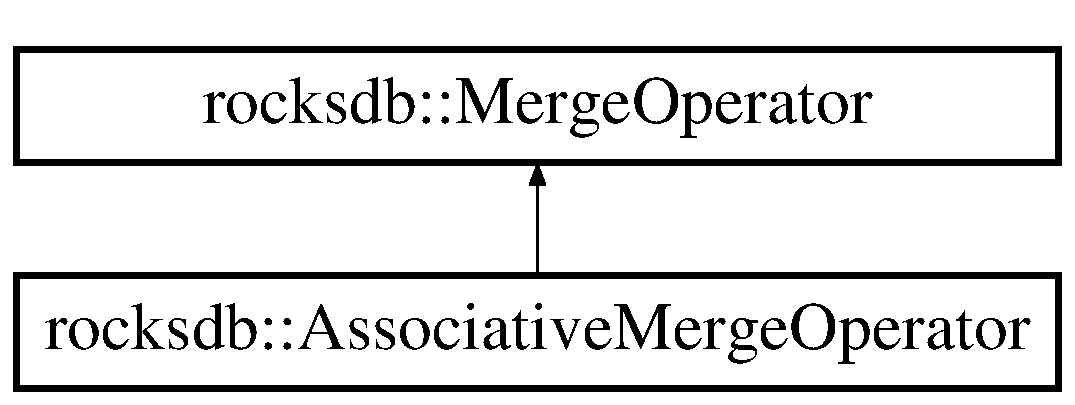
\includegraphics[height=2.000000cm]{classrocksdb_1_1AssociativeMergeOperator}
\end{center}
\end{figure}
\subsection*{Public Member Functions}
\begin{DoxyCompactItemize}
\item 
virtual bool {\bfseries Merge} (const \hyperlink{classrocksdb_1_1Slice}{Slice} \&key, const \hyperlink{classrocksdb_1_1Slice}{Slice} $\ast$existing\+\_\+value, const \hyperlink{classrocksdb_1_1Slice}{Slice} \&value, std\+::string $\ast$new\+\_\+value, \hyperlink{classrocksdb_1_1Logger}{Logger} $\ast$logger) const =0\hypertarget{classrocksdb_1_1AssociativeMergeOperator_a9a51ddbc04ad52a4ea4d15b252bead44}{}\label{classrocksdb_1_1AssociativeMergeOperator_a9a51ddbc04ad52a4ea4d15b252bead44}

\end{DoxyCompactItemize}


The documentation for this class was generated from the following file\+:\begin{DoxyCompactItemize}
\item 
Appserver/src/external/rocksdb/merge\+\_\+operator.\+h\end{DoxyCompactItemize}

\hypertarget{classrocksdb_1_1BackupableDB}{}\section{rocksdb\+:\+:Backupable\+DB Class Reference}
\label{classrocksdb_1_1BackupableDB}\index{rocksdb\+::\+Backupable\+DB@{rocksdb\+::\+Backupable\+DB}}
Inheritance diagram for rocksdb\+:\+:Backupable\+DB\+:\begin{figure}[H]
\begin{center}
\leavevmode
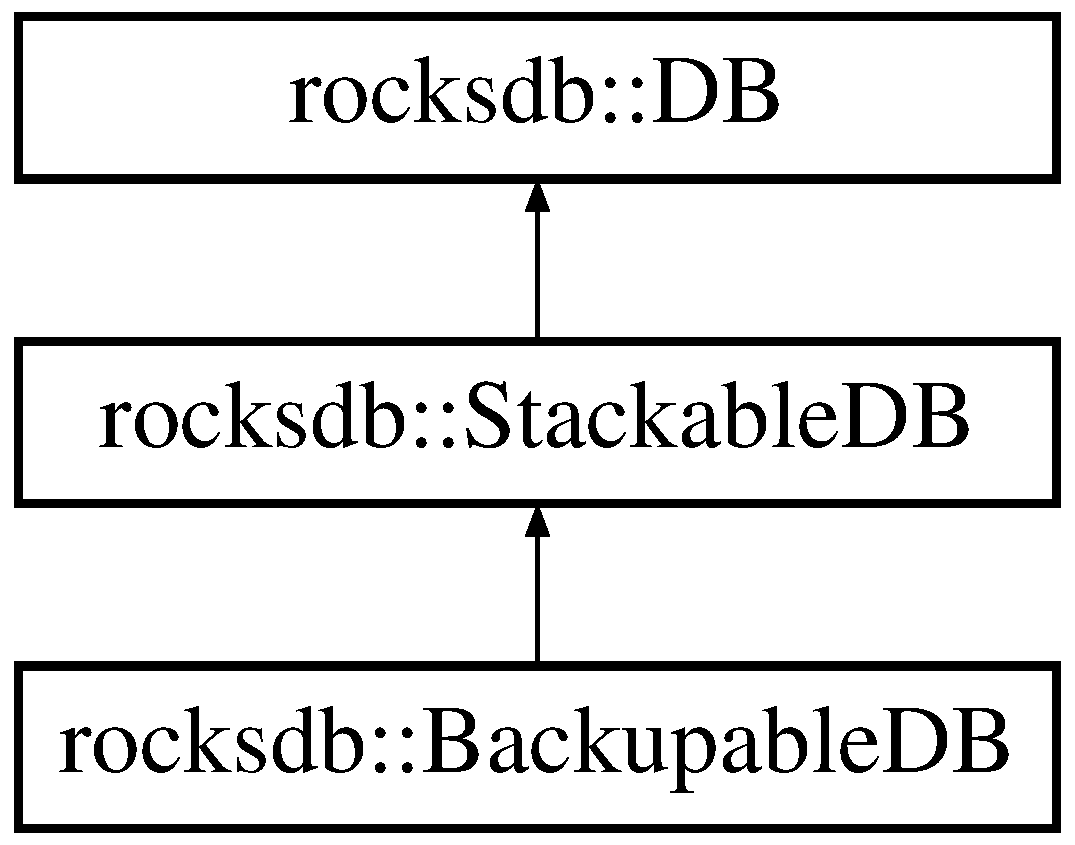
\includegraphics[height=3.000000cm]{classrocksdb_1_1BackupableDB}
\end{center}
\end{figure}
\subsection*{Public Member Functions}
\begin{DoxyCompactItemize}
\item 
{\bfseries Backupable\+DB} (\hyperlink{classrocksdb_1_1DB}{DB} $\ast$db, const \hyperlink{structrocksdb_1_1BackupableDBOptions}{Backupable\+D\+B\+Options} \&options)\hypertarget{classrocksdb_1_1BackupableDB_aec2a834e82c818b899afff3643042718}{}\label{classrocksdb_1_1BackupableDB_aec2a834e82c818b899afff3643042718}

\item 
\hyperlink{classrocksdb_1_1Status}{Status} {\bfseries Create\+New\+Backup} (bool flush\+\_\+before\+\_\+backup=false)\hypertarget{classrocksdb_1_1BackupableDB_ac04502c4cb1b1f0fd93f25a2306a6a6a}{}\label{classrocksdb_1_1BackupableDB_ac04502c4cb1b1f0fd93f25a2306a6a6a}

\item 
void {\bfseries Get\+Backup\+Info} (std\+::vector$<$ \hyperlink{structrocksdb_1_1BackupInfo}{Backup\+Info} $>$ $\ast$backup\+\_\+info)\hypertarget{classrocksdb_1_1BackupableDB_a723dd4de74025e89298e626c5d9df7c7}{}\label{classrocksdb_1_1BackupableDB_a723dd4de74025e89298e626c5d9df7c7}

\item 
void {\bfseries Get\+Corrupted\+Backups} (std\+::vector$<$ Backup\+ID $>$ $\ast$corrupt\+\_\+backup\+\_\+ids)\hypertarget{classrocksdb_1_1BackupableDB_ac8538fa3a90b261ab163bced63600d65}{}\label{classrocksdb_1_1BackupableDB_ac8538fa3a90b261ab163bced63600d65}

\item 
\hyperlink{classrocksdb_1_1Status}{Status} {\bfseries Purge\+Old\+Backups} (uint32\+\_\+t num\+\_\+backups\+\_\+to\+\_\+keep)\hypertarget{classrocksdb_1_1BackupableDB_aa8c1573be253f3626fc8665c57888733}{}\label{classrocksdb_1_1BackupableDB_aa8c1573be253f3626fc8665c57888733}

\item 
\hyperlink{classrocksdb_1_1Status}{Status} {\bfseries Delete\+Backup} (Backup\+ID backup\+\_\+id)\hypertarget{classrocksdb_1_1BackupableDB_aebece0f8d7b9d26e3fabef17c26d2fb4}{}\label{classrocksdb_1_1BackupableDB_aebece0f8d7b9d26e3fabef17c26d2fb4}

\item 
void {\bfseries Stop\+Backup} ()\hypertarget{classrocksdb_1_1BackupableDB_ad32d24faef144f48aa057a939a08a187}{}\label{classrocksdb_1_1BackupableDB_ad32d24faef144f48aa057a939a08a187}

\item 
\hyperlink{classrocksdb_1_1Status}{Status} {\bfseries Garbage\+Collect} ()\hypertarget{classrocksdb_1_1BackupableDB_a636cb6d47d92043adc97ea3a9c312ebb}{}\label{classrocksdb_1_1BackupableDB_a636cb6d47d92043adc97ea3a9c312ebb}

\end{DoxyCompactItemize}
\subsection*{Additional Inherited Members}


The documentation for this class was generated from the following file\+:\begin{DoxyCompactItemize}
\item 
Appserver/src/external/rocksdb/utilities/backupable\+\_\+db.\+h\end{DoxyCompactItemize}

\hypertarget{structrocksdb_1_1BackupableDBOptions}{}\section{rocksdb\+:\+:Backupable\+D\+B\+Options Struct Reference}
\label{structrocksdb_1_1BackupableDBOptions}\index{rocksdb\+::\+Backupable\+D\+B\+Options@{rocksdb\+::\+Backupable\+D\+B\+Options}}
\subsection*{Public Member Functions}
\begin{DoxyCompactItemize}
\item 
void {\bfseries Dump} (\hyperlink{classrocksdb_1_1Logger}{Logger} $\ast$logger) const\hypertarget{structrocksdb_1_1BackupableDBOptions_a22fe4956a960b3253d2f31d94d1109a0}{}\label{structrocksdb_1_1BackupableDBOptions_a22fe4956a960b3253d2f31d94d1109a0}

\item 
{\bfseries Backupable\+D\+B\+Options} (const std\+::string \&\+\_\+backup\+\_\+dir, \hyperlink{classrocksdb_1_1Env}{Env} $\ast$\+\_\+backup\+\_\+env=nullptr, bool \+\_\+share\+\_\+table\+\_\+files=true, \hyperlink{classrocksdb_1_1Logger}{Logger} $\ast$\+\_\+info\+\_\+log=nullptr, bool \+\_\+sync=true, bool \+\_\+destroy\+\_\+old\+\_\+data=false, bool \+\_\+backup\+\_\+log\+\_\+files=true, uint64\+\_\+t \+\_\+backup\+\_\+rate\+\_\+limit=0, uint64\+\_\+t \+\_\+restore\+\_\+rate\+\_\+limit=0, int \+\_\+max\+\_\+background\+\_\+operations=1, uint64\+\_\+t \+\_\+callback\+\_\+trigger\+\_\+interval\+\_\+size=4 $\ast$1024 $\ast$1024)\hypertarget{structrocksdb_1_1BackupableDBOptions_afa67e5c4be408333892a7ee328e48cd6}{}\label{structrocksdb_1_1BackupableDBOptions_afa67e5c4be408333892a7ee328e48cd6}

\end{DoxyCompactItemize}
\subsection*{Public Attributes}
\begin{DoxyCompactItemize}
\item 
std\+::string {\bfseries backup\+\_\+dir}\hypertarget{structrocksdb_1_1BackupableDBOptions_aa7a9e43a8609c0fd67594bb426ed7366}{}\label{structrocksdb_1_1BackupableDBOptions_aa7a9e43a8609c0fd67594bb426ed7366}

\item 
\hyperlink{classrocksdb_1_1Env}{Env} $\ast$ {\bfseries backup\+\_\+env}\hypertarget{structrocksdb_1_1BackupableDBOptions_aee6d3779b7aec87481c1926600fb3c93}{}\label{structrocksdb_1_1BackupableDBOptions_aee6d3779b7aec87481c1926600fb3c93}

\item 
bool {\bfseries share\+\_\+table\+\_\+files}\hypertarget{structrocksdb_1_1BackupableDBOptions_a8baef54d546cc200b5b466a66941b353}{}\label{structrocksdb_1_1BackupableDBOptions_a8baef54d546cc200b5b466a66941b353}

\item 
\hyperlink{classrocksdb_1_1Logger}{Logger} $\ast$ {\bfseries info\+\_\+log}\hypertarget{structrocksdb_1_1BackupableDBOptions_a9a9b781bcfd50d784167e875dd04db07}{}\label{structrocksdb_1_1BackupableDBOptions_a9a9b781bcfd50d784167e875dd04db07}

\item 
bool {\bfseries sync}\hypertarget{structrocksdb_1_1BackupableDBOptions_a86f1c6ef7eec4650a0dd2359435957a3}{}\label{structrocksdb_1_1BackupableDBOptions_a86f1c6ef7eec4650a0dd2359435957a3}

\item 
bool {\bfseries destroy\+\_\+old\+\_\+data}\hypertarget{structrocksdb_1_1BackupableDBOptions_ada8a43622c81102de20bd93649f14dd6}{}\label{structrocksdb_1_1BackupableDBOptions_ada8a43622c81102de20bd93649f14dd6}

\item 
bool {\bfseries backup\+\_\+log\+\_\+files}\hypertarget{structrocksdb_1_1BackupableDBOptions_abda4994d71ffd2096dcbef5be6406c3a}{}\label{structrocksdb_1_1BackupableDBOptions_abda4994d71ffd2096dcbef5be6406c3a}

\item 
uint64\+\_\+t {\bfseries backup\+\_\+rate\+\_\+limit}\hypertarget{structrocksdb_1_1BackupableDBOptions_add92a8bd33d695baefaa2725491c04e5}{}\label{structrocksdb_1_1BackupableDBOptions_add92a8bd33d695baefaa2725491c04e5}

\item 
uint64\+\_\+t {\bfseries restore\+\_\+rate\+\_\+limit}\hypertarget{structrocksdb_1_1BackupableDBOptions_ae3ad471d72bcde1f18ed8abb98dea54c}{}\label{structrocksdb_1_1BackupableDBOptions_ae3ad471d72bcde1f18ed8abb98dea54c}

\item 
bool {\bfseries share\+\_\+files\+\_\+with\+\_\+checksum}\hypertarget{structrocksdb_1_1BackupableDBOptions_a859edcb7ddb3d70c594b18b8d49f4620}{}\label{structrocksdb_1_1BackupableDBOptions_a859edcb7ddb3d70c594b18b8d49f4620}

\item 
int {\bfseries max\+\_\+background\+\_\+operations}\hypertarget{structrocksdb_1_1BackupableDBOptions_a80a0fdfbc03c6cac8d45bf9d136081d6}{}\label{structrocksdb_1_1BackupableDBOptions_a80a0fdfbc03c6cac8d45bf9d136081d6}

\item 
uint64\+\_\+t {\bfseries callback\+\_\+trigger\+\_\+interval\+\_\+size}\hypertarget{structrocksdb_1_1BackupableDBOptions_aea04efe346765be3010dee7b0bfec46c}{}\label{structrocksdb_1_1BackupableDBOptions_aea04efe346765be3010dee7b0bfec46c}

\end{DoxyCompactItemize}


The documentation for this struct was generated from the following file\+:\begin{DoxyCompactItemize}
\item 
Appserver/src/external/rocksdb/utilities/backupable\+\_\+db.\+h\end{DoxyCompactItemize}

\hypertarget{classrocksdb_1_1BackupEngine}{}\section{rocksdb\+:\+:Backup\+Engine Class Reference}
\label{classrocksdb_1_1BackupEngine}\index{rocksdb\+::\+Backup\+Engine@{rocksdb\+::\+Backup\+Engine}}
\subsection*{Public Member Functions}
\begin{DoxyCompactItemize}
\item 
virtual \hyperlink{classrocksdb_1_1Status}{Status} \hyperlink{classrocksdb_1_1BackupEngine_a334add83bac85feb928064dbee0f90b9}{Create\+New\+Backup\+With\+Metadata} (\hyperlink{classrocksdb_1_1DB}{DB} $\ast$db, const std\+::string \&app\+\_\+metadata, bool flush\+\_\+before\+\_\+backup=false, std\+::function$<$ void()$>$ progress\+\_\+callback=\mbox{[}$\,$\mbox{]}() \{\})=0\hypertarget{classrocksdb_1_1BackupEngine_a334add83bac85feb928064dbee0f90b9}{}\label{classrocksdb_1_1BackupEngine_a334add83bac85feb928064dbee0f90b9}

\begin{DoxyCompactList}\small\item\em same as Create\+New\+Backup, but stores extra application metadata \end{DoxyCompactList}\item 
virtual \hyperlink{classrocksdb_1_1Status}{Status} {\bfseries Create\+New\+Backup} (\hyperlink{classrocksdb_1_1DB}{DB} $\ast$db, bool flush\+\_\+before\+\_\+backup=false, std\+::function$<$ void()$>$ progress\+\_\+callback=\mbox{[}$\,$\mbox{]}() \{\})\hypertarget{classrocksdb_1_1BackupEngine_ae4caf7171f3980e4471d10eb784261bd}{}\label{classrocksdb_1_1BackupEngine_ae4caf7171f3980e4471d10eb784261bd}

\item 
virtual \hyperlink{classrocksdb_1_1Status}{Status} {\bfseries Purge\+Old\+Backups} (uint32\+\_\+t num\+\_\+backups\+\_\+to\+\_\+keep)=0\hypertarget{classrocksdb_1_1BackupEngine_a609107b69c9115182ac9e6007e971fc2}{}\label{classrocksdb_1_1BackupEngine_a609107b69c9115182ac9e6007e971fc2}

\item 
virtual \hyperlink{classrocksdb_1_1Status}{Status} {\bfseries Delete\+Backup} (Backup\+ID backup\+\_\+id)=0\hypertarget{classrocksdb_1_1BackupEngine_a92eebbe0e8a93221f2aadba43f0c426f}{}\label{classrocksdb_1_1BackupEngine_a92eebbe0e8a93221f2aadba43f0c426f}

\item 
virtual void {\bfseries Stop\+Backup} ()=0\hypertarget{classrocksdb_1_1BackupEngine_a9c8a34b3137c5c090c149cbff9fff8ee}{}\label{classrocksdb_1_1BackupEngine_a9c8a34b3137c5c090c149cbff9fff8ee}

\item 
virtual void {\bfseries Get\+Backup\+Info} (std\+::vector$<$ \hyperlink{structrocksdb_1_1BackupInfo}{Backup\+Info} $>$ $\ast$backup\+\_\+info)=0\hypertarget{classrocksdb_1_1BackupEngine_a52557124fa1a1c7dc1e0220b92d88064}{}\label{classrocksdb_1_1BackupEngine_a52557124fa1a1c7dc1e0220b92d88064}

\item 
virtual void {\bfseries Get\+Corrupted\+Backups} (std\+::vector$<$ Backup\+ID $>$ $\ast$corrupt\+\_\+backup\+\_\+ids)=0\hypertarget{classrocksdb_1_1BackupEngine_a702eb2e414abbf9faaf4065ef29c42e6}{}\label{classrocksdb_1_1BackupEngine_a702eb2e414abbf9faaf4065ef29c42e6}

\item 
virtual \hyperlink{classrocksdb_1_1Status}{Status} {\bfseries Restore\+D\+B\+From\+Backup} (Backup\+ID backup\+\_\+id, const std\+::string \&db\+\_\+dir, const std\+::string \&wal\+\_\+dir, const \hyperlink{structrocksdb_1_1RestoreOptions}{Restore\+Options} \&restore\+\_\+options=\hyperlink{structrocksdb_1_1RestoreOptions}{Restore\+Options}())=0\hypertarget{classrocksdb_1_1BackupEngine_a6ee696a103e180043b815d9446e0f1b4}{}\label{classrocksdb_1_1BackupEngine_a6ee696a103e180043b815d9446e0f1b4}

\item 
virtual \hyperlink{classrocksdb_1_1Status}{Status} {\bfseries Restore\+D\+B\+From\+Latest\+Backup} (const std\+::string \&db\+\_\+dir, const std\+::string \&wal\+\_\+dir, const \hyperlink{structrocksdb_1_1RestoreOptions}{Restore\+Options} \&restore\+\_\+options=\hyperlink{structrocksdb_1_1RestoreOptions}{Restore\+Options}())=0\hypertarget{classrocksdb_1_1BackupEngine_a42887e54bdc224558fb54202fad97c12}{}\label{classrocksdb_1_1BackupEngine_a42887e54bdc224558fb54202fad97c12}

\item 
virtual \hyperlink{classrocksdb_1_1Status}{Status} {\bfseries Verify\+Backup} (Backup\+ID backup\+\_\+id)=0\hypertarget{classrocksdb_1_1BackupEngine_aada26149e972ddce95827806ddd87aeb}{}\label{classrocksdb_1_1BackupEngine_aada26149e972ddce95827806ddd87aeb}

\item 
virtual \hyperlink{classrocksdb_1_1Status}{Status} {\bfseries Garbage\+Collect} ()=0\hypertarget{classrocksdb_1_1BackupEngine_a83526a443b363d59c68e93229c30a63a}{}\label{classrocksdb_1_1BackupEngine_a83526a443b363d59c68e93229c30a63a}

\end{DoxyCompactItemize}
\subsection*{Static Public Member Functions}
\begin{DoxyCompactItemize}
\item 
static \hyperlink{classrocksdb_1_1Status}{Status} {\bfseries Open} (\hyperlink{classrocksdb_1_1Env}{Env} $\ast$db\+\_\+env, const \hyperlink{structrocksdb_1_1BackupableDBOptions}{Backupable\+D\+B\+Options} \&options, \hyperlink{classrocksdb_1_1BackupEngine}{Backup\+Engine} $\ast$$\ast$backup\+\_\+engine\+\_\+ptr)\hypertarget{classrocksdb_1_1BackupEngine_a188d0f8e182da60f7670d9fb16beec12}{}\label{classrocksdb_1_1BackupEngine_a188d0f8e182da60f7670d9fb16beec12}

\end{DoxyCompactItemize}


The documentation for this class was generated from the following file\+:\begin{DoxyCompactItemize}
\item 
Appserver/src/external/rocksdb/utilities/backupable\+\_\+db.\+h\end{DoxyCompactItemize}

\hypertarget{classrocksdb_1_1BackupEngineReadOnly}{}\section{rocksdb\+:\+:Backup\+Engine\+Read\+Only Class Reference}
\label{classrocksdb_1_1BackupEngineReadOnly}\index{rocksdb\+::\+Backup\+Engine\+Read\+Only@{rocksdb\+::\+Backup\+Engine\+Read\+Only}}
\subsection*{Public Member Functions}
\begin{DoxyCompactItemize}
\item 
virtual void {\bfseries Get\+Backup\+Info} (std\+::vector$<$ \hyperlink{structrocksdb_1_1BackupInfo}{Backup\+Info} $>$ $\ast$backup\+\_\+info)=0\hypertarget{classrocksdb_1_1BackupEngineReadOnly_ab0fcb2fb57321bd8ad8f95bfec12b000}{}\label{classrocksdb_1_1BackupEngineReadOnly_ab0fcb2fb57321bd8ad8f95bfec12b000}

\item 
virtual void {\bfseries Get\+Corrupted\+Backups} (std\+::vector$<$ Backup\+ID $>$ $\ast$corrupt\+\_\+backup\+\_\+ids)=0\hypertarget{classrocksdb_1_1BackupEngineReadOnly_a12e6f7c1ac7db97dfa076b118fa7c3d6}{}\label{classrocksdb_1_1BackupEngineReadOnly_a12e6f7c1ac7db97dfa076b118fa7c3d6}

\item 
virtual \hyperlink{classrocksdb_1_1Status}{Status} {\bfseries Restore\+D\+B\+From\+Backup} (Backup\+ID backup\+\_\+id, const std\+::string \&db\+\_\+dir, const std\+::string \&wal\+\_\+dir, const \hyperlink{structrocksdb_1_1RestoreOptions}{Restore\+Options} \&restore\+\_\+options=\hyperlink{structrocksdb_1_1RestoreOptions}{Restore\+Options}())=0\hypertarget{classrocksdb_1_1BackupEngineReadOnly_aa86715641468f7db8869944189a66792}{}\label{classrocksdb_1_1BackupEngineReadOnly_aa86715641468f7db8869944189a66792}

\item 
virtual \hyperlink{classrocksdb_1_1Status}{Status} {\bfseries Restore\+D\+B\+From\+Latest\+Backup} (const std\+::string \&db\+\_\+dir, const std\+::string \&wal\+\_\+dir, const \hyperlink{structrocksdb_1_1RestoreOptions}{Restore\+Options} \&restore\+\_\+options=\hyperlink{structrocksdb_1_1RestoreOptions}{Restore\+Options}())=0\hypertarget{classrocksdb_1_1BackupEngineReadOnly_a1758914b174f7b0621f553f5bf6cab85}{}\label{classrocksdb_1_1BackupEngineReadOnly_a1758914b174f7b0621f553f5bf6cab85}

\item 
virtual \hyperlink{classrocksdb_1_1Status}{Status} {\bfseries Verify\+Backup} (Backup\+ID backup\+\_\+id)=0\hypertarget{classrocksdb_1_1BackupEngineReadOnly_a74dbf742dc27d7303851483fe242a2ae}{}\label{classrocksdb_1_1BackupEngineReadOnly_a74dbf742dc27d7303851483fe242a2ae}

\end{DoxyCompactItemize}
\subsection*{Static Public Member Functions}
\begin{DoxyCompactItemize}
\item 
static \hyperlink{classrocksdb_1_1Status}{Status} {\bfseries Open} (\hyperlink{classrocksdb_1_1Env}{Env} $\ast$db\+\_\+env, const \hyperlink{structrocksdb_1_1BackupableDBOptions}{Backupable\+D\+B\+Options} \&options, \hyperlink{classrocksdb_1_1BackupEngineReadOnly}{Backup\+Engine\+Read\+Only} $\ast$$\ast$backup\+\_\+engine\+\_\+ptr)\hypertarget{classrocksdb_1_1BackupEngineReadOnly_a22806e0fa2e1def361f722a07f95536a}{}\label{classrocksdb_1_1BackupEngineReadOnly_a22806e0fa2e1def361f722a07f95536a}

\end{DoxyCompactItemize}


The documentation for this class was generated from the following file\+:\begin{DoxyCompactItemize}
\item 
Appserver/src/external/rocksdb/utilities/backupable\+\_\+db.\+h\end{DoxyCompactItemize}

\hypertarget{structrocksdb_1_1BackupInfo}{}\section{rocksdb\+:\+:Backup\+Info Struct Reference}
\label{structrocksdb_1_1BackupInfo}\index{rocksdb\+::\+Backup\+Info@{rocksdb\+::\+Backup\+Info}}
\subsection*{Public Member Functions}
\begin{DoxyCompactItemize}
\item 
{\bfseries Backup\+Info} (Backup\+ID \+\_\+backup\+\_\+id, int64\+\_\+t \+\_\+timestamp, uint64\+\_\+t \+\_\+size, uint32\+\_\+t \+\_\+number\+\_\+files, const std\+::string \&\+\_\+app\+\_\+metadata)\hypertarget{structrocksdb_1_1BackupInfo_ae219e77d7a82852aae22f996af0a598e}{}\label{structrocksdb_1_1BackupInfo_ae219e77d7a82852aae22f996af0a598e}

\end{DoxyCompactItemize}
\subsection*{Public Attributes}
\begin{DoxyCompactItemize}
\item 
Backup\+ID {\bfseries backup\+\_\+id}\hypertarget{structrocksdb_1_1BackupInfo_ac694e575124d8da4e812979e1a7b7b17}{}\label{structrocksdb_1_1BackupInfo_ac694e575124d8da4e812979e1a7b7b17}

\item 
int64\+\_\+t {\bfseries timestamp}\hypertarget{structrocksdb_1_1BackupInfo_ab3b8e1719982fa30f57917e3d88896d9}{}\label{structrocksdb_1_1BackupInfo_ab3b8e1719982fa30f57917e3d88896d9}

\item 
uint64\+\_\+t {\bfseries size}\hypertarget{structrocksdb_1_1BackupInfo_a9e66561a83e7a131f501466b50cc40b0}{}\label{structrocksdb_1_1BackupInfo_a9e66561a83e7a131f501466b50cc40b0}

\item 
uint32\+\_\+t {\bfseries number\+\_\+files}\hypertarget{structrocksdb_1_1BackupInfo_a9c5878d45ea51109574bad353b984034}{}\label{structrocksdb_1_1BackupInfo_a9c5878d45ea51109574bad353b984034}

\item 
std\+::string {\bfseries app\+\_\+metadata}\hypertarget{structrocksdb_1_1BackupInfo_a56eeb6089379c3b71e59044fe7679167}{}\label{structrocksdb_1_1BackupInfo_a56eeb6089379c3b71e59044fe7679167}

\end{DoxyCompactItemize}


The documentation for this struct was generated from the following file\+:\begin{DoxyCompactItemize}
\item 
Appserver/src/external/rocksdb/utilities/backupable\+\_\+db.\+h\end{DoxyCompactItemize}

\hypertarget{classrocksdb_1_1BackupStatistics}{}\section{rocksdb\+:\+:Backup\+Statistics Class Reference}
\label{classrocksdb_1_1BackupStatistics}\index{rocksdb\+::\+Backup\+Statistics@{rocksdb\+::\+Backup\+Statistics}}
\subsection*{Public Member Functions}
\begin{DoxyCompactItemize}
\item 
{\bfseries Backup\+Statistics} (uint32\+\_\+t \+\_\+number\+\_\+success\+\_\+backup, uint32\+\_\+t \+\_\+number\+\_\+fail\+\_\+backup)\hypertarget{classrocksdb_1_1BackupStatistics_a7256228a765692e8ff75532b89c7b4a8}{}\label{classrocksdb_1_1BackupStatistics_a7256228a765692e8ff75532b89c7b4a8}

\item 
void {\bfseries Increment\+Number\+Success\+Backup} ()\hypertarget{classrocksdb_1_1BackupStatistics_a25cda07716dfe578672b4049adf7b7ea}{}\label{classrocksdb_1_1BackupStatistics_a25cda07716dfe578672b4049adf7b7ea}

\item 
void {\bfseries Increment\+Number\+Fail\+Backup} ()\hypertarget{classrocksdb_1_1BackupStatistics_ac0e5925e2bf1ee5e8b1b16555baba68b}{}\label{classrocksdb_1_1BackupStatistics_ac0e5925e2bf1ee5e8b1b16555baba68b}

\item 
uint32\+\_\+t {\bfseries Get\+Number\+Success\+Backup} () const\hypertarget{classrocksdb_1_1BackupStatistics_afe0f2000deb568c812c5c525ef9e942e}{}\label{classrocksdb_1_1BackupStatistics_afe0f2000deb568c812c5c525ef9e942e}

\item 
uint32\+\_\+t {\bfseries Get\+Number\+Fail\+Backup} () const\hypertarget{classrocksdb_1_1BackupStatistics_a74d26f5134cef2faa21e5e443d30c4c3}{}\label{classrocksdb_1_1BackupStatistics_a74d26f5134cef2faa21e5e443d30c4c3}

\item 
std\+::string {\bfseries To\+String} () const\hypertarget{classrocksdb_1_1BackupStatistics_a6a4e0c9f799367c506cc44ed0e4a1371}{}\label{classrocksdb_1_1BackupStatistics_a6a4e0c9f799367c506cc44ed0e4a1371}

\end{DoxyCompactItemize}


The documentation for this class was generated from the following file\+:\begin{DoxyCompactItemize}
\item 
Appserver/src/external/rocksdb/utilities/backupable\+\_\+db.\+h\end{DoxyCompactItemize}

\hypertarget{classBaseDeDatos}{}\section{Base\+De\+Datos Class Reference}
\label{classBaseDeDatos}\index{Base\+De\+Datos@{Base\+De\+Datos}}
\subsection*{Public Member Functions}
\begin{DoxyCompactItemize}
\item 
{\bfseries Base\+De\+Datos} (string ruta)\hypertarget{classBaseDeDatos_a31d33717618cea590d2dbb412d1ed76b}{}\label{classBaseDeDatos_a31d33717618cea590d2dbb412d1ed76b}

\item 
void {\bfseries put} (string clave, string valor)\hypertarget{classBaseDeDatos_ab3ddf5149897619dadc871fccf484b17}{}\label{classBaseDeDatos_ab3ddf5149897619dadc871fccf484b17}

\item 
string {\bfseries get} (string clave)\hypertarget{classBaseDeDatos_a2303f5c8884f7942ed7b1110924c43ff}{}\label{classBaseDeDatos_a2303f5c8884f7942ed7b1110924c43ff}

\item 
bool {\bfseries existe} (string clave)\hypertarget{classBaseDeDatos_a45d53eb6eb9803e9ef3c6cf8b4a69183}{}\label{classBaseDeDatos_a45d53eb6eb9803e9ef3c6cf8b4a69183}

\item 
void {\bfseries eliminar} (string clave)\hypertarget{classBaseDeDatos_a7c26f9c036a9c5d9b68618f700abc78f}{}\label{classBaseDeDatos_a7c26f9c036a9c5d9b68618f700abc78f}

\end{DoxyCompactItemize}


The documentation for this class was generated from the following files\+:\begin{DoxyCompactItemize}
\item 
Appserver/src/servicios/Base\+De\+Datos.\+h\item 
Appserver/src/servicios/Base\+De\+Datos.\+cpp\end{DoxyCompactItemize}

\hypertarget{structrocksdb_1_1BatchResult}{}\section{rocksdb\+:\+:Batch\+Result Struct Reference}
\label{structrocksdb_1_1BatchResult}\index{rocksdb\+::\+Batch\+Result@{rocksdb\+::\+Batch\+Result}}
\subsection*{Public Member Functions}
\begin{DoxyCompactItemize}
\item 
{\bfseries Batch\+Result} (const \hyperlink{structrocksdb_1_1BatchResult}{Batch\+Result} \&)=delete\hypertarget{structrocksdb_1_1BatchResult_ab8732507130b0933bed3ceb2cc2e10d2}{}\label{structrocksdb_1_1BatchResult_ab8732507130b0933bed3ceb2cc2e10d2}

\item 
\hyperlink{structrocksdb_1_1BatchResult}{Batch\+Result} \& {\bfseries operator=} (const \hyperlink{structrocksdb_1_1BatchResult}{Batch\+Result} \&)=delete\hypertarget{structrocksdb_1_1BatchResult_ad670fc1f443c873b2894c2012f453d2f}{}\label{structrocksdb_1_1BatchResult_ad670fc1f443c873b2894c2012f453d2f}

\item 
{\bfseries Batch\+Result} (\hyperlink{structrocksdb_1_1BatchResult}{Batch\+Result} \&\&b\+Result)\hypertarget{structrocksdb_1_1BatchResult_a6407a36281a89a9d84ee0d1a14484c2b}{}\label{structrocksdb_1_1BatchResult_a6407a36281a89a9d84ee0d1a14484c2b}

\item 
\hyperlink{structrocksdb_1_1BatchResult}{Batch\+Result} \& {\bfseries operator=} (\hyperlink{structrocksdb_1_1BatchResult}{Batch\+Result} \&\&b\+Result)\hypertarget{structrocksdb_1_1BatchResult_ad66b55d911c15a8462ee1fc027049c8a}{}\label{structrocksdb_1_1BatchResult_ad66b55d911c15a8462ee1fc027049c8a}

\end{DoxyCompactItemize}
\subsection*{Public Attributes}
\begin{DoxyCompactItemize}
\item 
Sequence\+Number {\bfseries sequence} = 0\hypertarget{structrocksdb_1_1BatchResult_a8a072e4c46c499c9aeab09f5f15724ad}{}\label{structrocksdb_1_1BatchResult_a8a072e4c46c499c9aeab09f5f15724ad}

\item 
std\+::unique\+\_\+ptr$<$ \hyperlink{classrocksdb_1_1WriteBatch}{Write\+Batch} $>$ {\bfseries write\+Batch\+Ptr}\hypertarget{structrocksdb_1_1BatchResult_a6873e4961934136bf279dc929235e9e9}{}\label{structrocksdb_1_1BatchResult_a6873e4961934136bf279dc929235e9e9}

\end{DoxyCompactItemize}


The documentation for this struct was generated from the following file\+:\begin{DoxyCompactItemize}
\item 
Appserver/src/external/rocksdb/transaction\+\_\+log.\+h\end{DoxyCompactItemize}

\hypertarget{structrocksdb_1_1BlockBasedTableOptions}{}\section{rocksdb\+:\+:Block\+Based\+Table\+Options Struct Reference}
\label{structrocksdb_1_1BlockBasedTableOptions}\index{rocksdb\+::\+Block\+Based\+Table\+Options@{rocksdb\+::\+Block\+Based\+Table\+Options}}
\subsection*{Public Types}
\begin{DoxyCompactItemize}
\item 
enum {\bfseries Index\+Type} \+: char \{ {\bfseries k\+Binary\+Search}, 
{\bfseries k\+Hash\+Search}
 \}\hypertarget{structrocksdb_1_1BlockBasedTableOptions_a93cf5570b2c1a10470db336b9d83e2ce}{}\label{structrocksdb_1_1BlockBasedTableOptions_a93cf5570b2c1a10470db336b9d83e2ce}

\end{DoxyCompactItemize}
\subsection*{Public Attributes}
\begin{DoxyCompactItemize}
\item 
std\+::shared\+\_\+ptr$<$ \hyperlink{classrocksdb_1_1FlushBlockPolicyFactory}{Flush\+Block\+Policy\+Factory} $>$ {\bfseries flush\+\_\+block\+\_\+policy\+\_\+factory}\hypertarget{structrocksdb_1_1BlockBasedTableOptions_ad73f8618a8e2f822a898b6b50351208a}{}\label{structrocksdb_1_1BlockBasedTableOptions_ad73f8618a8e2f822a898b6b50351208a}

\item 
bool {\bfseries cache\+\_\+index\+\_\+and\+\_\+filter\+\_\+blocks} = false\hypertarget{structrocksdb_1_1BlockBasedTableOptions_a9b47fc5e2871d2928b6b4c6bffe6017c}{}\label{structrocksdb_1_1BlockBasedTableOptions_a9b47fc5e2871d2928b6b4c6bffe6017c}

\item 
bool {\bfseries pin\+\_\+l0\+\_\+filter\+\_\+and\+\_\+index\+\_\+blocks\+\_\+in\+\_\+cache} = false\hypertarget{structrocksdb_1_1BlockBasedTableOptions_ac711b41f7055cdae0e3554b57bfe114f}{}\label{structrocksdb_1_1BlockBasedTableOptions_ac711b41f7055cdae0e3554b57bfe114f}

\item 
Index\+Type {\bfseries index\+\_\+type} = k\+Binary\+Search\hypertarget{structrocksdb_1_1BlockBasedTableOptions_ae00971fc952135fe87df4f9f041e5289}{}\label{structrocksdb_1_1BlockBasedTableOptions_ae00971fc952135fe87df4f9f041e5289}

\item 
bool {\bfseries hash\+\_\+index\+\_\+allow\+\_\+collision} = true\hypertarget{structrocksdb_1_1BlockBasedTableOptions_a1404fa6a494624d4dca4038e06312003}{}\label{structrocksdb_1_1BlockBasedTableOptions_a1404fa6a494624d4dca4038e06312003}

\item 
Checksum\+Type {\bfseries checksum} = k\+C\+R\+C32c\hypertarget{structrocksdb_1_1BlockBasedTableOptions_a1adc5994a69a8cd0e1647148d0c2f752}{}\label{structrocksdb_1_1BlockBasedTableOptions_a1adc5994a69a8cd0e1647148d0c2f752}

\item 
bool {\bfseries no\+\_\+block\+\_\+cache} = false\hypertarget{structrocksdb_1_1BlockBasedTableOptions_ae3a1448054303148e9c1d73c0d3a8149}{}\label{structrocksdb_1_1BlockBasedTableOptions_ae3a1448054303148e9c1d73c0d3a8149}

\item 
std\+::shared\+\_\+ptr$<$ \hyperlink{classrocksdb_1_1Cache}{Cache} $>$ {\bfseries block\+\_\+cache} = nullptr\hypertarget{structrocksdb_1_1BlockBasedTableOptions_af7012b6cfc023265669ca3db6fd8a6ac}{}\label{structrocksdb_1_1BlockBasedTableOptions_af7012b6cfc023265669ca3db6fd8a6ac}

\item 
std\+::shared\+\_\+ptr$<$ \hyperlink{classrocksdb_1_1Cache}{Cache} $>$ {\bfseries block\+\_\+cache\+\_\+compressed} = nullptr\hypertarget{structrocksdb_1_1BlockBasedTableOptions_a333d1974b959b500e643e73d42f079f2}{}\label{structrocksdb_1_1BlockBasedTableOptions_a333d1974b959b500e643e73d42f079f2}

\item 
size\+\_\+t {\bfseries block\+\_\+size} = 4 $\ast$ 1024\hypertarget{structrocksdb_1_1BlockBasedTableOptions_ac6d52bc1b24b8420aa8565be69d8c503}{}\label{structrocksdb_1_1BlockBasedTableOptions_ac6d52bc1b24b8420aa8565be69d8c503}

\item 
int {\bfseries block\+\_\+size\+\_\+deviation} = 10\hypertarget{structrocksdb_1_1BlockBasedTableOptions_ad32cd3d71e1f30b9962a7c8de3cc16e5}{}\label{structrocksdb_1_1BlockBasedTableOptions_ad32cd3d71e1f30b9962a7c8de3cc16e5}

\item 
int {\bfseries block\+\_\+restart\+\_\+interval} = 16\hypertarget{structrocksdb_1_1BlockBasedTableOptions_a8bd604aaca756ab9e6308c8b198283ef}{}\label{structrocksdb_1_1BlockBasedTableOptions_a8bd604aaca756ab9e6308c8b198283ef}

\item 
int {\bfseries index\+\_\+block\+\_\+restart\+\_\+interval} = 1\hypertarget{structrocksdb_1_1BlockBasedTableOptions_a23a65c7cba2b2b44386cceb5b2077604}{}\label{structrocksdb_1_1BlockBasedTableOptions_a23a65c7cba2b2b44386cceb5b2077604}

\item 
bool {\bfseries use\+\_\+delta\+\_\+encoding} = true\hypertarget{structrocksdb_1_1BlockBasedTableOptions_a115eda587a9b226a49c662310fc66fae}{}\label{structrocksdb_1_1BlockBasedTableOptions_a115eda587a9b226a49c662310fc66fae}

\item 
std\+::shared\+\_\+ptr$<$ const \hyperlink{classrocksdb_1_1FilterPolicy}{Filter\+Policy} $>$ {\bfseries filter\+\_\+policy} = nullptr\hypertarget{structrocksdb_1_1BlockBasedTableOptions_accd96f660a1807c81d9f29fa56bfaa7c}{}\label{structrocksdb_1_1BlockBasedTableOptions_accd96f660a1807c81d9f29fa56bfaa7c}

\item 
bool {\bfseries whole\+\_\+key\+\_\+filtering} = true\hypertarget{structrocksdb_1_1BlockBasedTableOptions_a28ac408b75f3a8ce18174ef0314790cb}{}\label{structrocksdb_1_1BlockBasedTableOptions_a28ac408b75f3a8ce18174ef0314790cb}

\item 
bool {\bfseries skip\+\_\+table\+\_\+builder\+\_\+flush} = false\hypertarget{structrocksdb_1_1BlockBasedTableOptions_a9134bd76833f7acda42d5ed177f94b62}{}\label{structrocksdb_1_1BlockBasedTableOptions_a9134bd76833f7acda42d5ed177f94b62}

\item 
uint32\+\_\+t {\bfseries format\+\_\+version} = 2\hypertarget{structrocksdb_1_1BlockBasedTableOptions_a6c14b0303d48e4d6a2ceec75b2d4e0ae}{}\label{structrocksdb_1_1BlockBasedTableOptions_a6c14b0303d48e4d6a2ceec75b2d4e0ae}

\end{DoxyCompactItemize}


The documentation for this struct was generated from the following file\+:\begin{DoxyCompactItemize}
\item 
Appserver/src/external/rocksdb/table.\+h\end{DoxyCompactItemize}

\hypertarget{structrocksdb_1_1BlockBasedTablePropertyNames}{}\section{rocksdb\+:\+:Block\+Based\+Table\+Property\+Names Struct Reference}
\label{structrocksdb_1_1BlockBasedTablePropertyNames}\index{rocksdb\+::\+Block\+Based\+Table\+Property\+Names@{rocksdb\+::\+Block\+Based\+Table\+Property\+Names}}
\subsection*{Static Public Attributes}
\begin{DoxyCompactItemize}
\item 
static const std\+::string {\bfseries k\+Index\+Type}\hypertarget{structrocksdb_1_1BlockBasedTablePropertyNames_a68daf9a0361536f691e0a3e2130c2f05}{}\label{structrocksdb_1_1BlockBasedTablePropertyNames_a68daf9a0361536f691e0a3e2130c2f05}

\item 
static const std\+::string {\bfseries k\+Whole\+Key\+Filtering}\hypertarget{structrocksdb_1_1BlockBasedTablePropertyNames_aa2616d9324ec0ff90fc797f7fd93eb54}{}\label{structrocksdb_1_1BlockBasedTablePropertyNames_aa2616d9324ec0ff90fc797f7fd93eb54}

\item 
static const std\+::string {\bfseries k\+Prefix\+Filtering}\hypertarget{structrocksdb_1_1BlockBasedTablePropertyNames_a58b9db16091e5cdf6d790d4616b26562}{}\label{structrocksdb_1_1BlockBasedTablePropertyNames_a58b9db16091e5cdf6d790d4616b26562}

\end{DoxyCompactItemize}


The documentation for this struct was generated from the following file\+:\begin{DoxyCompactItemize}
\item 
Appserver/src/external/rocksdb/table.\+h\end{DoxyCompactItemize}

\hypertarget{structrocksdb_1_1spatial_1_1BoundingBox}{}\section{rocksdb\+:\+:spatial\+:\+:Bounding\+Box$<$ T $>$ Struct Template Reference}
\label{structrocksdb_1_1spatial_1_1BoundingBox}\index{rocksdb\+::spatial\+::\+Bounding\+Box$<$ T $>$@{rocksdb\+::spatial\+::\+Bounding\+Box$<$ T $>$}}
\subsection*{Public Member Functions}
\begin{DoxyCompactItemize}
\item 
{\bfseries Bounding\+Box} (T \+\_\+min\+\_\+x, T \+\_\+min\+\_\+y, T \+\_\+max\+\_\+x, T \+\_\+max\+\_\+y)\hypertarget{structrocksdb_1_1spatial_1_1BoundingBox_a7ce735b4eecba1f6b2a83651f0b0b9f8}{}\label{structrocksdb_1_1spatial_1_1BoundingBox_a7ce735b4eecba1f6b2a83651f0b0b9f8}

\item 
bool {\bfseries Intersects} (const \hyperlink{structrocksdb_1_1spatial_1_1BoundingBox}{Bounding\+Box}$<$ T $>$ \&a) const\hypertarget{structrocksdb_1_1spatial_1_1BoundingBox_a25981c6ad8bbf6c457955fae70d112fa}{}\label{structrocksdb_1_1spatial_1_1BoundingBox_a25981c6ad8bbf6c457955fae70d112fa}

\end{DoxyCompactItemize}
\subsection*{Public Attributes}
\begin{DoxyCompactItemize}
\item 
T {\bfseries min\+\_\+x}\hypertarget{structrocksdb_1_1spatial_1_1BoundingBox_a26416337084e7b54df9eec78fb9f9439}{}\label{structrocksdb_1_1spatial_1_1BoundingBox_a26416337084e7b54df9eec78fb9f9439}

\item 
T {\bfseries min\+\_\+y}\hypertarget{structrocksdb_1_1spatial_1_1BoundingBox_af3902f573fe67e6ed8550c944c6b4540}{}\label{structrocksdb_1_1spatial_1_1BoundingBox_af3902f573fe67e6ed8550c944c6b4540}

\item 
T {\bfseries max\+\_\+x}\hypertarget{structrocksdb_1_1spatial_1_1BoundingBox_aa19c5cc39d97e71260a71cee09ffa4cf}{}\label{structrocksdb_1_1spatial_1_1BoundingBox_aa19c5cc39d97e71260a71cee09ffa4cf}

\item 
T {\bfseries max\+\_\+y}\hypertarget{structrocksdb_1_1spatial_1_1BoundingBox_aafdfa0fc1ffc2f3b8a3d114b0bf3258d}{}\label{structrocksdb_1_1spatial_1_1BoundingBox_aafdfa0fc1ffc2f3b8a3d114b0bf3258d}

\end{DoxyCompactItemize}


The documentation for this struct was generated from the following file\+:\begin{DoxyCompactItemize}
\item 
Appserver/src/external/rocksdb/utilities/spatial\+\_\+db.\+h\end{DoxyCompactItemize}

\hypertarget{structJson_1_1BuiltStyledStreamWriter}{}\section{Json\+:\+:Built\+Styled\+Stream\+Writer Struct Reference}
\label{structJson_1_1BuiltStyledStreamWriter}\index{Json\+::\+Built\+Styled\+Stream\+Writer@{Json\+::\+Built\+Styled\+Stream\+Writer}}
Inheritance diagram for Json\+:\+:Built\+Styled\+Stream\+Writer\+:\begin{figure}[H]
\begin{center}
\leavevmode
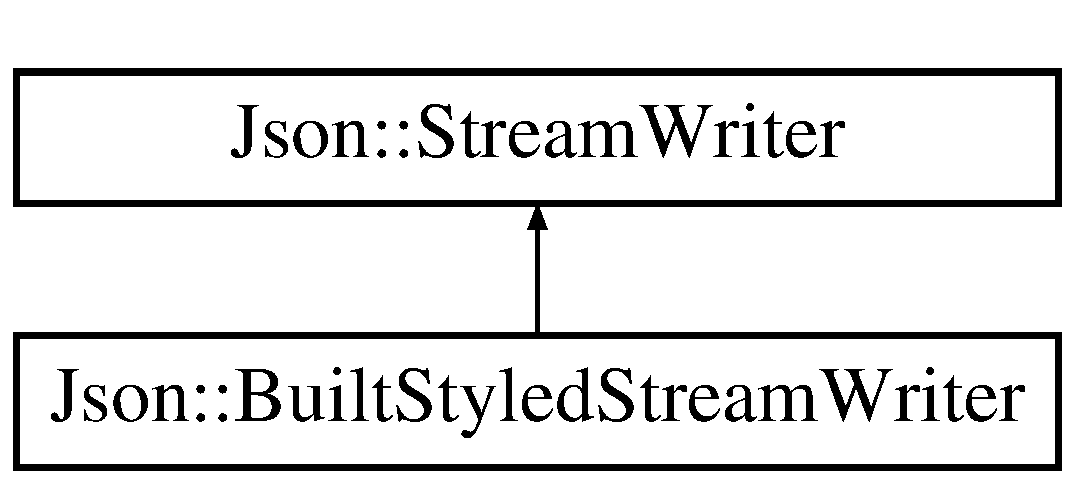
\includegraphics[height=2.000000cm]{structJson_1_1BuiltStyledStreamWriter}
\end{center}
\end{figure}
\subsection*{Public Member Functions}
\begin{DoxyCompactItemize}
\item 
{\bfseries Built\+Styled\+Stream\+Writer} (J\+S\+O\+N\+C\+P\+P\+\_\+\+S\+T\+R\+I\+NG const \&indentation, \hyperlink{structJson_1_1CommentStyle_a51fc08f3518fd81eba12f340d19a3d0c}{Comment\+Style\+::\+Enum} cs, J\+S\+O\+N\+C\+P\+P\+\_\+\+S\+T\+R\+I\+NG const \&colon\+Symbol, J\+S\+O\+N\+C\+P\+P\+\_\+\+S\+T\+R\+I\+NG const \&null\+Symbol, J\+S\+O\+N\+C\+P\+P\+\_\+\+S\+T\+R\+I\+NG const \&ending\+Line\+Feed\+Symbol, bool use\+Special\+Floats, unsigned int precision)\hypertarget{structJson_1_1BuiltStyledStreamWriter_adf11b7d1ee3c68d096b7c662ee85948e}{}\label{structJson_1_1BuiltStyledStreamWriter_adf11b7d1ee3c68d096b7c662ee85948e}

\item 
int \hyperlink{structJson_1_1BuiltStyledStreamWriter_a823cdb1afabb6b0d5f39bcd5a6a6f747}{write} (\hyperlink{classJson_1_1Value}{Value} const \&root, J\+S\+O\+N\+C\+P\+P\+\_\+\+O\+S\+T\+R\+E\+AM $\ast$sout) J\+S\+O\+N\+C\+P\+P\+\_\+\+O\+V\+E\+R\+R\+I\+DE
\end{DoxyCompactItemize}
\subsection*{Additional Inherited Members}


\subsection{Member Function Documentation}
\index{Json\+::\+Built\+Styled\+Stream\+Writer@{Json\+::\+Built\+Styled\+Stream\+Writer}!write@{write}}
\index{write@{write}!Json\+::\+Built\+Styled\+Stream\+Writer@{Json\+::\+Built\+Styled\+Stream\+Writer}}
\subsubsection[{\texorpdfstring{write(\+Value const \&root, J\+S\+O\+N\+C\+P\+P\+\_\+\+O\+S\+T\+R\+E\+A\+M $\ast$sout) J\+S\+O\+N\+C\+P\+P\+\_\+\+O\+V\+E\+R\+R\+I\+DE}{write(Value const \&root, JSONCPP\_OSTREAM *sout) JSONCPP\_OVERRIDE}}]{\setlength{\rightskip}{0pt plus 5cm}int Json\+::\+Built\+Styled\+Stream\+Writer\+::write (
\begin{DoxyParamCaption}
\item[{{\bf Value} const \&}]{root, }
\item[{J\+S\+O\+N\+C\+P\+P\+\_\+\+O\+S\+T\+R\+E\+AM $\ast$}]{sout}
\end{DoxyParamCaption}
)\hspace{0.3cm}{\ttfamily [virtual]}}\hypertarget{structJson_1_1BuiltStyledStreamWriter_a823cdb1afabb6b0d5f39bcd5a6a6f747}{}\label{structJson_1_1BuiltStyledStreamWriter_a823cdb1afabb6b0d5f39bcd5a6a6f747}
Write \hyperlink{classJson_1_1Value}{Value} into document as configured in sub-\/class. Do not take ownership of sout, but maintain a reference during function. \begin{DoxyPrecond}{Precondition}
sout != N\+U\+LL 
\end{DoxyPrecond}
\begin{DoxyReturn}{Returns}
zero on success (For now, we always return zero, so check the stream instead.) 
\end{DoxyReturn}

\begin{DoxyExceptions}{Exceptions}
{\em std\+::exception} & possibly, depending on configuration \\
\hline
\end{DoxyExceptions}


Implements \hyperlink{classJson_1_1StreamWriter_a84278bad0c9a9fc587bc2a97c5bb5993}{Json\+::\+Stream\+Writer}.



The documentation for this struct was generated from the following file\+:\begin{DoxyCompactItemize}
\item 
Appserver/src/external/json/jsoncpp.\+cpp\end{DoxyCompactItemize}

\hypertarget{classrocksdb_1_1Cache}{}\section{rocksdb\+:\+:Cache Class Reference}
\label{classrocksdb_1_1Cache}\index{rocksdb\+::\+Cache@{rocksdb\+::\+Cache}}
\subsection*{Classes}
\begin{DoxyCompactItemize}
\item 
struct \hyperlink{structrocksdb_1_1Cache_1_1Handle}{Handle}
\end{DoxyCompactItemize}
\subsection*{Public Member Functions}
\begin{DoxyCompactItemize}
\item 
virtual \hyperlink{classrocksdb_1_1Status}{Status} {\bfseries Insert} (const \hyperlink{classrocksdb_1_1Slice}{Slice} \&key, void $\ast$value, size\+\_\+t charge, void($\ast$deleter)(const \hyperlink{classrocksdb_1_1Slice}{Slice} \&key, void $\ast$value), \hyperlink{structrocksdb_1_1Cache_1_1Handle}{Handle} $\ast$$\ast$handle=nullptr)=0\hypertarget{classrocksdb_1_1Cache_aeeb1f83d19acd5e1dd08509361d17fd1}{}\label{classrocksdb_1_1Cache_aeeb1f83d19acd5e1dd08509361d17fd1}

\item 
virtual \hyperlink{structrocksdb_1_1Cache_1_1Handle}{Handle} $\ast$ {\bfseries Lookup} (const \hyperlink{classrocksdb_1_1Slice}{Slice} \&key)=0\hypertarget{classrocksdb_1_1Cache_a3df9823558cb3e87be72a61d494601d8}{}\label{classrocksdb_1_1Cache_a3df9823558cb3e87be72a61d494601d8}

\item 
virtual void {\bfseries Release} (\hyperlink{structrocksdb_1_1Cache_1_1Handle}{Handle} $\ast$handle)=0\hypertarget{classrocksdb_1_1Cache_a0c407981dfc226d8ec65e6b076aab42d}{}\label{classrocksdb_1_1Cache_a0c407981dfc226d8ec65e6b076aab42d}

\item 
virtual void $\ast$ {\bfseries Value} (\hyperlink{structrocksdb_1_1Cache_1_1Handle}{Handle} $\ast$handle)=0\hypertarget{classrocksdb_1_1Cache_a18ed26fd1e9e7097fea1a8ee3b2599b4}{}\label{classrocksdb_1_1Cache_a18ed26fd1e9e7097fea1a8ee3b2599b4}

\item 
virtual void {\bfseries Erase} (const \hyperlink{classrocksdb_1_1Slice}{Slice} \&key)=0\hypertarget{classrocksdb_1_1Cache_a17a30d33adccef40afe04ce729f7a2f2}{}\label{classrocksdb_1_1Cache_a17a30d33adccef40afe04ce729f7a2f2}

\item 
virtual uint64\+\_\+t {\bfseries New\+Id} ()=0\hypertarget{classrocksdb_1_1Cache_a0f53cd36aae877c68a28d128734a2b4a}{}\label{classrocksdb_1_1Cache_a0f53cd36aae877c68a28d128734a2b4a}

\item 
virtual void {\bfseries Set\+Capacity} (size\+\_\+t capacity)=0\hypertarget{classrocksdb_1_1Cache_a752de19d361112a191f61f5fcb47758d}{}\label{classrocksdb_1_1Cache_a752de19d361112a191f61f5fcb47758d}

\item 
virtual void {\bfseries Set\+Strict\+Capacity\+Limit} (bool strict\+\_\+capacity\+\_\+limit)=0\hypertarget{classrocksdb_1_1Cache_a241b2e3c50e9cdfa53733cb5f7d8e899}{}\label{classrocksdb_1_1Cache_a241b2e3c50e9cdfa53733cb5f7d8e899}

\item 
virtual bool {\bfseries Has\+Strict\+Capacity\+Limit} () const =0\hypertarget{classrocksdb_1_1Cache_ae54a9d537e7f71412a0c77f5aef21746}{}\label{classrocksdb_1_1Cache_ae54a9d537e7f71412a0c77f5aef21746}

\item 
virtual size\+\_\+t {\bfseries Get\+Capacity} () const =0\hypertarget{classrocksdb_1_1Cache_accff305fc4e6553a09fe543b7fed62d4}{}\label{classrocksdb_1_1Cache_accff305fc4e6553a09fe543b7fed62d4}

\item 
virtual size\+\_\+t {\bfseries Get\+Usage} () const =0\hypertarget{classrocksdb_1_1Cache_ab37eee9208f9fee29c929e47e3f9d9b8}{}\label{classrocksdb_1_1Cache_ab37eee9208f9fee29c929e47e3f9d9b8}

\item 
virtual size\+\_\+t {\bfseries Get\+Usage} (\hyperlink{structrocksdb_1_1Cache_1_1Handle}{Handle} $\ast$handle) const =0\hypertarget{classrocksdb_1_1Cache_a5130bfdcc04fe4e3485261058e6fb1de}{}\label{classrocksdb_1_1Cache_a5130bfdcc04fe4e3485261058e6fb1de}

\item 
virtual size\+\_\+t {\bfseries Get\+Pinned\+Usage} () const =0\hypertarget{classrocksdb_1_1Cache_ade4d9d95b99efa035727abaa29350625}{}\label{classrocksdb_1_1Cache_ade4d9d95b99efa035727abaa29350625}

\item 
virtual void {\bfseries Disown\+Data} ()\hypertarget{classrocksdb_1_1Cache_ad91007b91bd80c31bc6aac392874ba19}{}\label{classrocksdb_1_1Cache_ad91007b91bd80c31bc6aac392874ba19}

\item 
virtual void {\bfseries Apply\+To\+All\+Cache\+Entries} (void($\ast$callback)(void $\ast$, size\+\_\+t), bool thread\+\_\+safe)=0\hypertarget{classrocksdb_1_1Cache_a83bf8ca591a3b1fddb503c6f2fbe0994}{}\label{classrocksdb_1_1Cache_a83bf8ca591a3b1fddb503c6f2fbe0994}

\item 
virtual void {\bfseries Erase\+Un\+Ref\+Entries} ()=0\hypertarget{classrocksdb_1_1Cache_a045e94f30862a1821358a9fb277eba0e}{}\label{classrocksdb_1_1Cache_a045e94f30862a1821358a9fb277eba0e}

\end{DoxyCompactItemize}


The documentation for this class was generated from the following file\+:\begin{DoxyCompactItemize}
\item 
Appserver/src/external/rocksdb/cache.\+h\end{DoxyCompactItemize}

\hypertarget{classCandidatos}{}\section{Candidatos Class Reference}
\label{classCandidatos}\index{Candidatos@{Candidatos}}
\subsection*{Public Member Functions}
\begin{DoxyCompactItemize}
\item 
{\bfseries Candidatos} (string ruta)\hypertarget{classCandidatos_addc453f8a4be61234502e37b70855c52}{}\label{classCandidatos_addc453f8a4be61234502e37b70855c52}

\item 
void {\bfseries registrar\+Notificacion\+A\+Usuario\+Sobre\+Candidato} (string usuario, string candidato)\hypertarget{classCandidatos_a7eea8f2e1a19d605678588f482b97b08}{}\label{classCandidatos_a7eea8f2e1a19d605678588f482b97b08}

\item 
bool {\bfseries usuario\+Fue\+Notificado\+Sobre\+El\+Candidato} (string usuario, string candidato)\hypertarget{classCandidatos_abb4837245d85e28e2b86ae05e133b310}{}\label{classCandidatos_abb4837245d85e28e2b86ae05e133b310}

\item 
bool {\bfseries usuario\+Vota\+A\+Favor\+De} (string usuario1, string usuario2, bool voto\+A\+Favor)\hypertarget{classCandidatos_acb549bd56eefbc3c6f0f9cffd1a75f29}{}\label{classCandidatos_acb549bd56eefbc3c6f0f9cffd1a75f29}

\item 
bool {\bfseries hay\+Match\+Entre} (string usuario1, string usuario2)\hypertarget{classCandidatos_a3d96ff8c128d242975635a9839046f7b}{}\label{classCandidatos_a3d96ff8c128d242975635a9839046f7b}

\end{DoxyCompactItemize}


The documentation for this class was generated from the following files\+:\begin{DoxyCompactItemize}
\item 
Appserver/src/servicios/Candidatos.\+h\item 
Appserver/src/servicios/Candidatos.\+cpp\end{DoxyCompactItemize}

\hypertarget{unionchar64long16}{}\section{char64long16 Union Reference}
\label{unionchar64long16}\index{char64long16@{char64long16}}
\subsection*{Public Attributes}
\begin{DoxyCompactItemize}
\item 
unsigned char {\bfseries c} \mbox{[}64\mbox{]}\hypertarget{unionchar64long16_a7067dbe3b0ff3f11661acb8cd97bcff9}{}\label{unionchar64long16_a7067dbe3b0ff3f11661acb8cd97bcff9}

\item 
uint32\+\_\+t {\bfseries l} \mbox{[}16\mbox{]}\hypertarget{unionchar64long16_a4f1edebae3468a551ff2d0cdaecb467d}{}\label{unionchar64long16_a4f1edebae3468a551ff2d0cdaecb467d}

\end{DoxyCompactItemize}


The documentation for this union was generated from the following file\+:\begin{DoxyCompactItemize}
\item 
Appserver/src/external/mongoose/mongoose.\+c\end{DoxyCompactItemize}

\hypertarget{classJson_1_1CharReader}{}\section{Json\+:\+:Char\+Reader Class Reference}
\label{classJson_1_1CharReader}\index{Json\+::\+Char\+Reader@{Json\+::\+Char\+Reader}}


{\ttfamily \#include $<$json.\+h$>$}

Inheritance diagram for Json\+:\+:Char\+Reader\+:\begin{figure}[H]
\begin{center}
\leavevmode
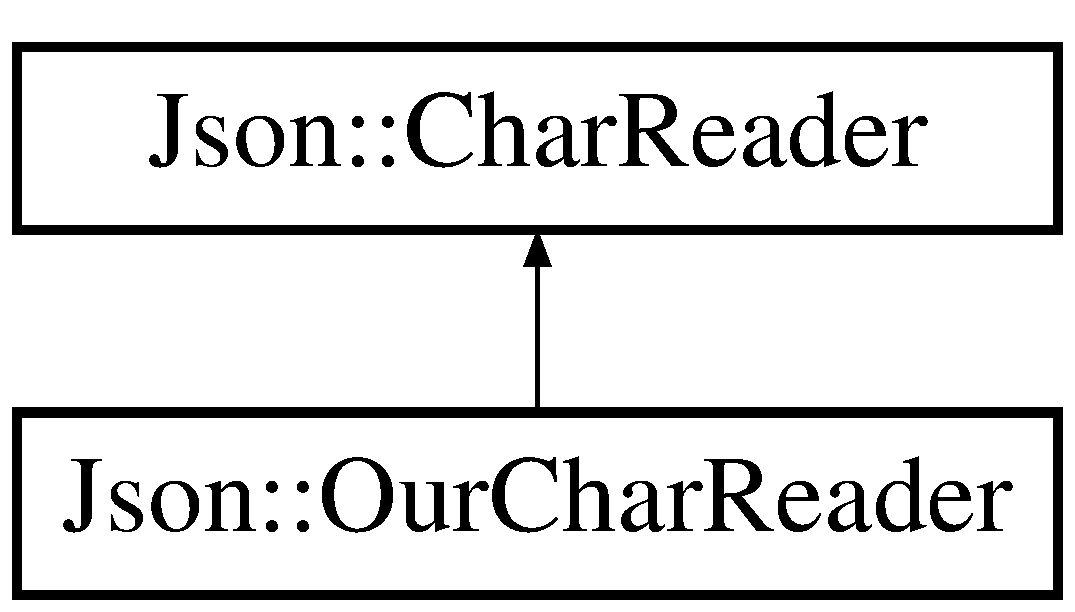
\includegraphics[height=2.000000cm]{classJson_1_1CharReader}
\end{center}
\end{figure}
\subsection*{Classes}
\begin{DoxyCompactItemize}
\item 
class \hyperlink{classJson_1_1CharReader_1_1Factory}{Factory}
\end{DoxyCompactItemize}
\subsection*{Public Member Functions}
\begin{DoxyCompactItemize}
\item 
virtual bool \hyperlink{classJson_1_1CharReader_a7983680d50fd0745f371c43b162e78e1}{parse} (char const $\ast$begin\+Doc, char const $\ast$end\+Doc, \hyperlink{classJson_1_1Value}{Value} $\ast$root, J\+S\+O\+N\+C\+P\+P\+\_\+\+S\+T\+R\+I\+NG $\ast$errs)=0
\begin{DoxyCompactList}\small\item\em Read a \hyperlink{classJson_1_1Value}{Value} from a \href{http://www.json.org}{\tt J\+S\+ON} document. The document must be a U\+T\+F-\/8 encoded string containing the document to read. \end{DoxyCompactList}\end{DoxyCompactItemize}


\subsection{Detailed Description}
Interface for reading J\+S\+ON from a char array. 

\subsection{Member Function Documentation}
\index{Json\+::\+Char\+Reader@{Json\+::\+Char\+Reader}!parse@{parse}}
\index{parse@{parse}!Json\+::\+Char\+Reader@{Json\+::\+Char\+Reader}}
\subsubsection[{\texorpdfstring{parse(char const $\ast$begin\+Doc, char const $\ast$end\+Doc, Value $\ast$root, J\+S\+O\+N\+C\+P\+P\+\_\+\+S\+T\+R\+I\+N\+G $\ast$errs)=0}{parse(char const *beginDoc, char const *endDoc, Value *root, JSONCPP\_STRING *errs)=0}}]{\setlength{\rightskip}{0pt plus 5cm}virtual bool Json\+::\+Char\+Reader\+::parse (
\begin{DoxyParamCaption}
\item[{char const $\ast$}]{begin\+Doc, }
\item[{char const $\ast$}]{end\+Doc, }
\item[{{\bf Value} $\ast$}]{root, }
\item[{J\+S\+O\+N\+C\+P\+P\+\_\+\+S\+T\+R\+I\+NG $\ast$}]{errs}
\end{DoxyParamCaption}
)\hspace{0.3cm}{\ttfamily [pure virtual]}}\hypertarget{classJson_1_1CharReader_a7983680d50fd0745f371c43b162e78e1}{}\label{classJson_1_1CharReader_a7983680d50fd0745f371c43b162e78e1}


Read a \hyperlink{classJson_1_1Value}{Value} from a \href{http://www.json.org}{\tt J\+S\+ON} document. The document must be a U\+T\+F-\/8 encoded string containing the document to read. 


\begin{DoxyParams}{Parameters}
{\em begin\+Doc} & Pointer on the beginning of the U\+T\+F-\/8 encoded string of the document to read. \\
\hline
{\em end\+Doc} & Pointer on the end of the U\+T\+F-\/8 encoded string of the document to read. Must be $>$= begin\+Doc. \\
\hline
{\em root} & \mbox{[}out\mbox{]} Contains the root value of the document if it was successfully parsed. \\
\hline
{\em errs} & \mbox{[}out\mbox{]} Formatted error messages (if not N\+U\+LL) a user friendly string that lists errors in the parsed document. \\
\hline
\end{DoxyParams}
\begin{DoxyReturn}{Returns}
{\ttfamily true} if the document was successfully parsed, {\ttfamily false} if an error occurred. 
\end{DoxyReturn}


Implemented in \hyperlink{classJson_1_1OurCharReader_a547f08ec5a9951ca69e8bb2e90296c83}{Json\+::\+Our\+Char\+Reader}.



The documentation for this class was generated from the following file\+:\begin{DoxyCompactItemize}
\item 
Appserver/src/external/json/json.\+h\end{DoxyCompactItemize}

\hypertarget{classJson_1_1CharReaderBuilder}{}\section{Json\+:\+:Char\+Reader\+Builder Class Reference}
\label{classJson_1_1CharReaderBuilder}\index{Json\+::\+Char\+Reader\+Builder@{Json\+::\+Char\+Reader\+Builder}}


Build a \hyperlink{classJson_1_1CharReader}{Char\+Reader} implementation.  




{\ttfamily \#include $<$json.\+h$>$}

Inheritance diagram for Json\+:\+:Char\+Reader\+Builder\+:\begin{figure}[H]
\begin{center}
\leavevmode
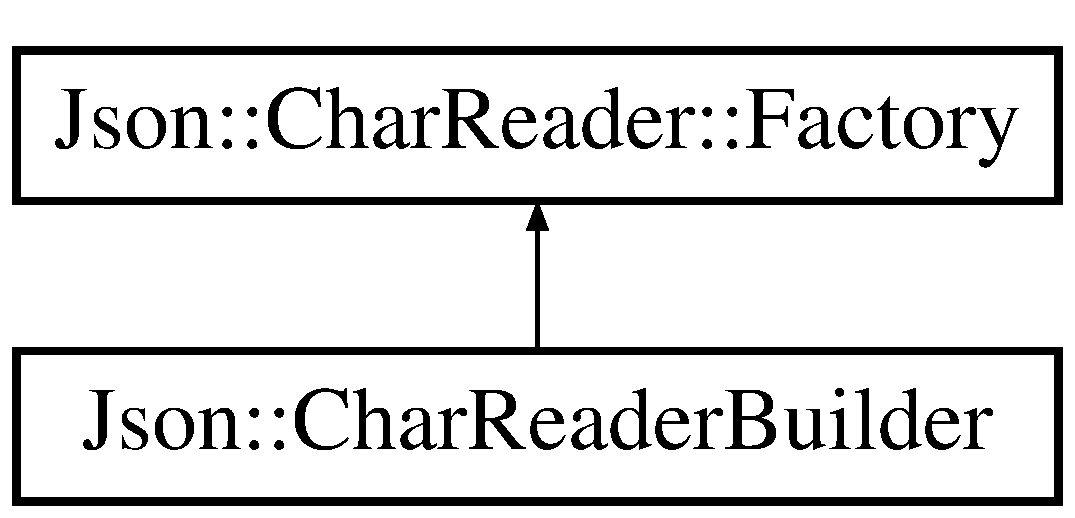
\includegraphics[height=2.000000cm]{classJson_1_1CharReaderBuilder}
\end{center}
\end{figure}
\subsection*{Public Member Functions}
\begin{DoxyCompactItemize}
\item 
\hyperlink{classJson_1_1CharReader}{Char\+Reader} $\ast$ \hyperlink{classJson_1_1CharReaderBuilder_a3a262fcc76c1eb8eebfd4718fb4e9722}{new\+Char\+Reader} () const J\+S\+O\+N\+C\+P\+P\+\_\+\+O\+V\+E\+R\+R\+I\+DE
\begin{DoxyCompactList}\small\item\em Allocate a \hyperlink{classJson_1_1CharReader}{Char\+Reader} via operator new(). \end{DoxyCompactList}\item 
bool \hyperlink{classJson_1_1CharReaderBuilder_af890b5cb70e9b372e41de5c9e6535d21}{validate} (\hyperlink{classJson_1_1Value}{Json\+::\+Value} $\ast$invalid) const
\item 
\hyperlink{classJson_1_1Value}{Value} \& \hyperlink{classJson_1_1CharReaderBuilder_a84b35ef443340c06c0aa7b47851d8d86}{operator\mbox{[}$\,$\mbox{]}} (J\+S\+O\+N\+C\+P\+P\+\_\+\+S\+T\+R\+I\+NG key)
\end{DoxyCompactItemize}
\subsection*{Static Public Member Functions}
\begin{DoxyCompactItemize}
\item 
static void \hyperlink{classJson_1_1CharReaderBuilder_a03ff031e06aabff989ab4addc87294ab}{set\+Defaults} (\hyperlink{classJson_1_1Value}{Json\+::\+Value} $\ast$settings)
\item 
static void \hyperlink{classJson_1_1CharReaderBuilder_a9c19e3c5475f9072d527810d4bf56749}{strict\+Mode} (\hyperlink{classJson_1_1Value}{Json\+::\+Value} $\ast$settings)
\end{DoxyCompactItemize}
\subsection*{Public Attributes}
\begin{DoxyCompactItemize}
\item 
\hyperlink{classJson_1_1Value}{Json\+::\+Value} \hyperlink{classJson_1_1CharReaderBuilder_ac69b7911ad64c171c51ebaf2ea26d958}{settings\+\_\+}
\end{DoxyCompactItemize}


\subsection{Detailed Description}
Build a \hyperlink{classJson_1_1CharReader}{Char\+Reader} implementation. 

Usage\+: 
\begin{DoxyCode}
\textcolor{keyword}{using namespace }\hyperlink{namespaceJson}{Json};
\hyperlink{classJson_1_1CharReaderBuilder}{CharReaderBuilder} builder;
builder[\textcolor{stringliteral}{"collectComments"}] = \textcolor{keyword}{false};
\hyperlink{classJson_1_1Value}{Value} value;
JSONCPP\_STRING errs;
\textcolor{keywordtype}{bool} ok = \hyperlink{namespaceJson_aab0cf1ecf81d1aeca12be2a416a84352}{parseFromStream}(builder, std::cin, &value, &errs);
\end{DoxyCode}
 

\subsection{Member Function Documentation}
\index{Json\+::\+Char\+Reader\+Builder@{Json\+::\+Char\+Reader\+Builder}!new\+Char\+Reader@{new\+Char\+Reader}}
\index{new\+Char\+Reader@{new\+Char\+Reader}!Json\+::\+Char\+Reader\+Builder@{Json\+::\+Char\+Reader\+Builder}}
\subsubsection[{\texorpdfstring{new\+Char\+Reader() const J\+S\+O\+N\+C\+P\+P\+\_\+\+O\+V\+E\+R\+R\+I\+DE}{newCharReader() const JSONCPP\_OVERRIDE}}]{\setlength{\rightskip}{0pt plus 5cm}{\bf Char\+Reader} $\ast$ Json\+::\+Char\+Reader\+Builder\+::new\+Char\+Reader (
\begin{DoxyParamCaption}
{}
\end{DoxyParamCaption}
) const\hspace{0.3cm}{\ttfamily [virtual]}}\hypertarget{classJson_1_1CharReaderBuilder_a3a262fcc76c1eb8eebfd4718fb4e9722}{}\label{classJson_1_1CharReaderBuilder_a3a262fcc76c1eb8eebfd4718fb4e9722}


Allocate a \hyperlink{classJson_1_1CharReader}{Char\+Reader} via operator new(). 


\begin{DoxyExceptions}{Exceptions}
{\em std\+::exception} & if something goes wrong (e.\+g. invalid settings) \\
\hline
\end{DoxyExceptions}


Implements \hyperlink{classJson_1_1CharReader_1_1Factory_a4c5862a1ffd432372dbe65cf59de98c4}{Json\+::\+Char\+Reader\+::\+Factory}.

\index{Json\+::\+Char\+Reader\+Builder@{Json\+::\+Char\+Reader\+Builder}!operator\mbox{[}$\,$\mbox{]}@{operator[]}}
\index{operator\mbox{[}$\,$\mbox{]}@{operator[]}!Json\+::\+Char\+Reader\+Builder@{Json\+::\+Char\+Reader\+Builder}}
\subsubsection[{\texorpdfstring{operator[](\+J\+S\+O\+N\+C\+P\+P\+\_\+\+S\+T\+R\+I\+N\+G key)}{operator[](JSONCPP\_STRING key)}}]{\setlength{\rightskip}{0pt plus 5cm}{\bf Value} \& Json\+::\+Char\+Reader\+Builder\+::operator\mbox{[}$\,$\mbox{]} (
\begin{DoxyParamCaption}
\item[{J\+S\+O\+N\+C\+P\+P\+\_\+\+S\+T\+R\+I\+NG}]{key}
\end{DoxyParamCaption}
)}\hypertarget{classJson_1_1CharReaderBuilder_a84b35ef443340c06c0aa7b47851d8d86}{}\label{classJson_1_1CharReaderBuilder_a84b35ef443340c06c0aa7b47851d8d86}
A simple way to update a specific setting. \index{Json\+::\+Char\+Reader\+Builder@{Json\+::\+Char\+Reader\+Builder}!set\+Defaults@{set\+Defaults}}
\index{set\+Defaults@{set\+Defaults}!Json\+::\+Char\+Reader\+Builder@{Json\+::\+Char\+Reader\+Builder}}
\subsubsection[{\texorpdfstring{set\+Defaults(\+Json\+::\+Value $\ast$settings)}{setDefaults(Json::Value *settings)}}]{\setlength{\rightskip}{0pt plus 5cm}void Json\+::\+Char\+Reader\+Builder\+::set\+Defaults (
\begin{DoxyParamCaption}
\item[{{\bf Json\+::\+Value} $\ast$}]{settings}
\end{DoxyParamCaption}
)\hspace{0.3cm}{\ttfamily [static]}}\hypertarget{classJson_1_1CharReaderBuilder_a03ff031e06aabff989ab4addc87294ab}{}\label{classJson_1_1CharReaderBuilder_a03ff031e06aabff989ab4addc87294ab}
Called by ctor, but you can use this to reset settings\+\_\+. \begin{DoxyPrecond}{Precondition}
\textquotesingle{}settings\textquotesingle{} != N\+U\+LL (but Json\+::null is fine) 
\end{DoxyPrecond}
\begin{DoxyRemark}{Remarks}
Defaults\+: 
\begin{DoxyCodeInclude}
\end{DoxyCodeInclude}

\end{DoxyRemark}
\mbox{[}Char\+Reader\+Builder\+Defaults\mbox{]}

\mbox{[}Char\+Reader\+Builder\+Defaults\mbox{]} \index{Json\+::\+Char\+Reader\+Builder@{Json\+::\+Char\+Reader\+Builder}!strict\+Mode@{strict\+Mode}}
\index{strict\+Mode@{strict\+Mode}!Json\+::\+Char\+Reader\+Builder@{Json\+::\+Char\+Reader\+Builder}}
\subsubsection[{\texorpdfstring{strict\+Mode(\+Json\+::\+Value $\ast$settings)}{strictMode(Json::Value *settings)}}]{\setlength{\rightskip}{0pt plus 5cm}void Json\+::\+Char\+Reader\+Builder\+::strict\+Mode (
\begin{DoxyParamCaption}
\item[{{\bf Json\+::\+Value} $\ast$}]{settings}
\end{DoxyParamCaption}
)\hspace{0.3cm}{\ttfamily [static]}}\hypertarget{classJson_1_1CharReaderBuilder_a9c19e3c5475f9072d527810d4bf56749}{}\label{classJson_1_1CharReaderBuilder_a9c19e3c5475f9072d527810d4bf56749}
Same as old \hyperlink{classJson_1_1Features_ae23176c14b2e79e81fb61fb1a8ab58ee}{Features\+::strict\+Mode()}. \begin{DoxyPrecond}{Precondition}
\textquotesingle{}settings\textquotesingle{} != N\+U\+LL (but Json\+::null is fine) 
\end{DoxyPrecond}
\begin{DoxyRemark}{Remarks}
Defaults\+: 
\begin{DoxyCodeInclude}
\end{DoxyCodeInclude}

\end{DoxyRemark}
\mbox{[}Char\+Reader\+Builder\+Strict\+Mode\mbox{]}

\mbox{[}Char\+Reader\+Builder\+Strict\+Mode\mbox{]} \index{Json\+::\+Char\+Reader\+Builder@{Json\+::\+Char\+Reader\+Builder}!validate@{validate}}
\index{validate@{validate}!Json\+::\+Char\+Reader\+Builder@{Json\+::\+Char\+Reader\+Builder}}
\subsubsection[{\texorpdfstring{validate(\+Json\+::\+Value $\ast$invalid) const}{validate(Json::Value *invalid) const}}]{\setlength{\rightskip}{0pt plus 5cm}bool Json\+::\+Char\+Reader\+Builder\+::validate (
\begin{DoxyParamCaption}
\item[{{\bf Json\+::\+Value} $\ast$}]{invalid}
\end{DoxyParamCaption}
) const}\hypertarget{classJson_1_1CharReaderBuilder_af890b5cb70e9b372e41de5c9e6535d21}{}\label{classJson_1_1CharReaderBuilder_af890b5cb70e9b372e41de5c9e6535d21}
\begin{DoxyReturn}{Returns}
true if \textquotesingle{}settings\textquotesingle{} are legal and consistent; otherwise, indicate bad settings via \textquotesingle{}invalid\textquotesingle{}. 
\end{DoxyReturn}


\subsection{Member Data Documentation}
\index{Json\+::\+Char\+Reader\+Builder@{Json\+::\+Char\+Reader\+Builder}!settings\+\_\+@{settings\+\_\+}}
\index{settings\+\_\+@{settings\+\_\+}!Json\+::\+Char\+Reader\+Builder@{Json\+::\+Char\+Reader\+Builder}}
\subsubsection[{\texorpdfstring{settings\+\_\+}{settings\_}}]{\setlength{\rightskip}{0pt plus 5cm}{\bf Json\+::\+Value} Json\+::\+Char\+Reader\+Builder\+::settings\+\_\+}\hypertarget{classJson_1_1CharReaderBuilder_ac69b7911ad64c171c51ebaf2ea26d958}{}\label{classJson_1_1CharReaderBuilder_ac69b7911ad64c171c51ebaf2ea26d958}
Configuration of this builder. These are case-\/sensitive. Available settings (case-\/sensitive)\+:
\begin{DoxyItemize}
\item {\ttfamily \char`\"{}collect\+Comments\char`\"{}\+: false or true}
\begin{DoxyItemize}
\item true to collect comment and allow writing them back during serialization, false to discard comments. This parameter is ignored if allow\+Comments is false.
\end{DoxyItemize}
\item {\ttfamily \char`\"{}allow\+Comments\char`\"{}\+: false or true}
\begin{DoxyItemize}
\item true if comments are allowed.
\end{DoxyItemize}
\item {\ttfamily \char`\"{}strict\+Root\char`\"{}\+: false or true}
\begin{DoxyItemize}
\item true if root must be either an array or an object value
\end{DoxyItemize}
\item {\ttfamily \char`\"{}allow\+Dropped\+Null\+Placeholders\char`\"{}\+: false or true}
\begin{DoxyItemize}
\item true if dropped null placeholders are allowed. (See \hyperlink{classJson_1_1StreamWriterBuilder}{Stream\+Writer\+Builder}.)
\end{DoxyItemize}
\item {\ttfamily \char`\"{}allow\+Numeric\+Keys\char`\"{}\+: false or true}
\begin{DoxyItemize}
\item true if numeric object keys are allowed.
\end{DoxyItemize}
\item {\ttfamily \char`\"{}allow\+Single\+Quotes\char`\"{}\+: false or true}
\begin{DoxyItemize}
\item true if \textquotesingle{}\textquotesingle{} are allowed for strings (both keys and values)
\end{DoxyItemize}
\item {\ttfamily \char`\"{}stack\+Limit\char`\"{}\+: integer}
\begin{DoxyItemize}
\item Exceeding stack\+Limit (recursive depth of {\ttfamily read\+Value()}) will cause an exception.
\item This is a security issue (seg-\/faults caused by deeply nested J\+S\+ON), so the default is low.
\end{DoxyItemize}
\item {\ttfamily \char`\"{}fail\+If\+Extra\char`\"{}\+: false or true}
\begin{DoxyItemize}
\item If true, {\ttfamily parse()} returns false when extra non-\/whitespace trails the J\+S\+ON value in the input string.
\end{DoxyItemize}
\item {\ttfamily \char`\"{}reject\+Dup\+Keys\char`\"{}\+: false or true}
\begin{DoxyItemize}
\item If true, {\ttfamily parse()} returns false when a key is duplicated within an object.
\end{DoxyItemize}
\item {\ttfamily \char`\"{}allow\+Special\+Floats\char`\"{}\+: false or true}
\begin{DoxyItemize}
\item If true, special float values (Na\+Ns and infinities) are allowed and their values are lossfree restorable.
\end{DoxyItemize}
\end{DoxyItemize}

You can examine \textquotesingle{}settings\+\_\+` yourself to see the defaults. You can also write and read them just like any J\+S\+ON \hyperlink{classJson_1_1Value}{Value}. \begin{DoxySeeAlso}{See also}
\hyperlink{classJson_1_1CharReaderBuilder_a03ff031e06aabff989ab4addc87294ab}{set\+Defaults()} 
\end{DoxySeeAlso}


The documentation for this class was generated from the following files\+:\begin{DoxyCompactItemize}
\item 
Appserver/src/external/json/json.\+h\item 
Appserver/src/external/json/jsoncpp.\+cpp\end{DoxyCompactItemize}

\hypertarget{classrocksdb_1_1Checkpoint}{}\section{rocksdb\+:\+:Checkpoint Class Reference}
\label{classrocksdb_1_1Checkpoint}\index{rocksdb\+::\+Checkpoint@{rocksdb\+::\+Checkpoint}}
\subsection*{Public Member Functions}
\begin{DoxyCompactItemize}
\item 
virtual \hyperlink{classrocksdb_1_1Status}{Status} {\bfseries Create\+Checkpoint} (const std\+::string \&checkpoint\+\_\+dir)\hypertarget{classrocksdb_1_1Checkpoint_ac635f7a56467bce415edeac6faafd25b}{}\label{classrocksdb_1_1Checkpoint_ac635f7a56467bce415edeac6faafd25b}

\end{DoxyCompactItemize}
\subsection*{Static Public Member Functions}
\begin{DoxyCompactItemize}
\item 
static \hyperlink{classrocksdb_1_1Status}{Status} {\bfseries Create} (\hyperlink{classrocksdb_1_1DB}{DB} $\ast$db, \hyperlink{classrocksdb_1_1Checkpoint}{Checkpoint} $\ast$$\ast$checkpoint\+\_\+ptr)\hypertarget{classrocksdb_1_1Checkpoint_a063a95e7832b0faa2e54e92ade9b0123}{}\label{classrocksdb_1_1Checkpoint_a063a95e7832b0faa2e54e92ade9b0123}

\end{DoxyCompactItemize}


The documentation for this class was generated from the following file\+:\begin{DoxyCompactItemize}
\item 
Appserver/src/external/rocksdb/utilities/checkpoint.\+h\end{DoxyCompactItemize}

\hypertarget{classrocksdb_1_1Cleanable}{}\section{rocksdb\+:\+:Cleanable Class Reference}
\label{classrocksdb_1_1Cleanable}\index{rocksdb\+::\+Cleanable@{rocksdb\+::\+Cleanable}}
Inheritance diagram for rocksdb\+:\+:Cleanable\+:\begin{figure}[H]
\begin{center}
\leavevmode
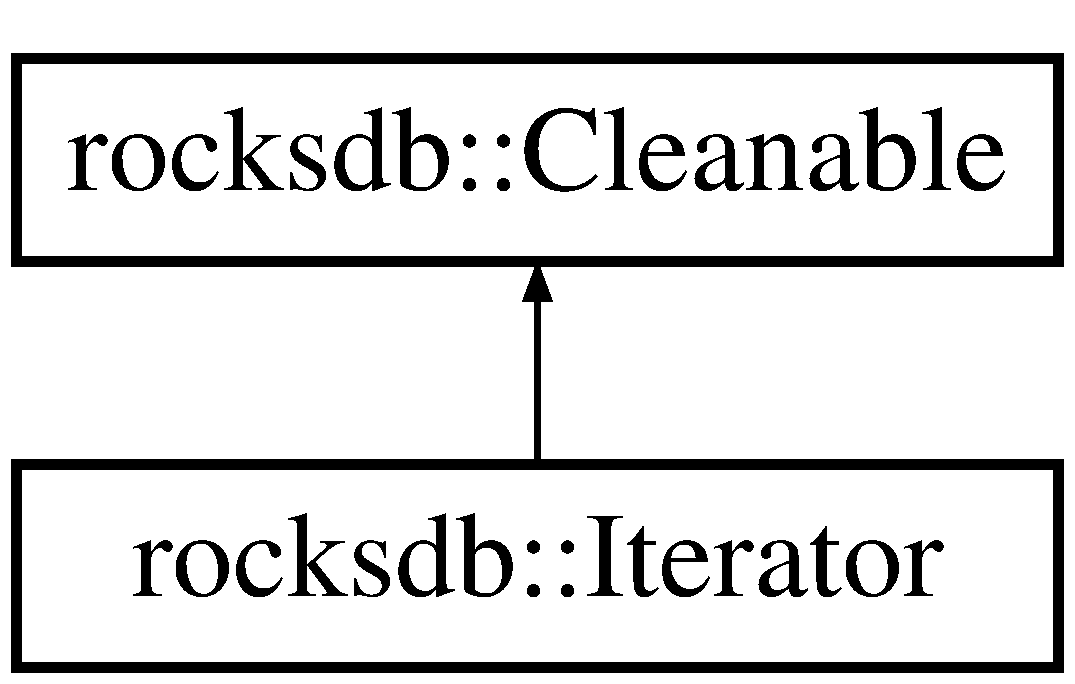
\includegraphics[height=2.000000cm]{classrocksdb_1_1Cleanable}
\end{center}
\end{figure}
\subsection*{Classes}
\begin{DoxyCompactItemize}
\item 
struct \hyperlink{structrocksdb_1_1Cleanable_1_1Cleanup}{Cleanup}
\end{DoxyCompactItemize}
\subsection*{Public Types}
\begin{DoxyCompactItemize}
\item 
typedef void($\ast$ {\bfseries Cleanup\+Function}) (void $\ast$arg1, void $\ast$arg2)\hypertarget{classrocksdb_1_1Cleanable_a68bb2c33e6b54bc0e510aecc81095913}{}\label{classrocksdb_1_1Cleanable_a68bb2c33e6b54bc0e510aecc81095913}

\end{DoxyCompactItemize}
\subsection*{Public Member Functions}
\begin{DoxyCompactItemize}
\item 
void {\bfseries Register\+Cleanup} (Cleanup\+Function function, void $\ast$arg1, void $\ast$arg2)\hypertarget{classrocksdb_1_1Cleanable_ac848cc814e5f42f6b5a909a75a12351f}{}\label{classrocksdb_1_1Cleanable_ac848cc814e5f42f6b5a909a75a12351f}

\end{DoxyCompactItemize}
\subsection*{Protected Attributes}
\begin{DoxyCompactItemize}
\item 
\hyperlink{structrocksdb_1_1Cleanable_1_1Cleanup}{Cleanup} {\bfseries cleanup\+\_\+}\hypertarget{classrocksdb_1_1Cleanable_ab874a5c66ee637057de636b53c1883c0}{}\label{classrocksdb_1_1Cleanable_ab874a5c66ee637057de636b53c1883c0}

\end{DoxyCompactItemize}


The documentation for this class was generated from the following file\+:\begin{DoxyCompactItemize}
\item 
Appserver/src/external/rocksdb/iterator.\+h\end{DoxyCompactItemize}

\hypertarget{structrocksdb_1_1Cleanable_1_1Cleanup}{}\section{rocksdb\+:\+:Cleanable\+:\+:Cleanup Struct Reference}
\label{structrocksdb_1_1Cleanable_1_1Cleanup}\index{rocksdb\+::\+Cleanable\+::\+Cleanup@{rocksdb\+::\+Cleanable\+::\+Cleanup}}
\subsection*{Public Attributes}
\begin{DoxyCompactItemize}
\item 
Cleanup\+Function {\bfseries function}\hypertarget{structrocksdb_1_1Cleanable_1_1Cleanup_a3dd70245f1a3adb8c71c2fe05aafcd0e}{}\label{structrocksdb_1_1Cleanable_1_1Cleanup_a3dd70245f1a3adb8c71c2fe05aafcd0e}

\item 
void $\ast$ {\bfseries arg1}\hypertarget{structrocksdb_1_1Cleanable_1_1Cleanup_a2aa0ab56c7c4f9fd3c56e8d28dfae94e}{}\label{structrocksdb_1_1Cleanable_1_1Cleanup_a2aa0ab56c7c4f9fd3c56e8d28dfae94e}

\item 
void $\ast$ {\bfseries arg2}\hypertarget{structrocksdb_1_1Cleanable_1_1Cleanup_a663dba13cc20c0544a2cc7e192c8de8d}{}\label{structrocksdb_1_1Cleanable_1_1Cleanup_a663dba13cc20c0544a2cc7e192c8de8d}

\item 
\hyperlink{structrocksdb_1_1Cleanable_1_1Cleanup}{Cleanup} $\ast$ {\bfseries next}\hypertarget{structrocksdb_1_1Cleanable_1_1Cleanup_a7abe56c85a97991623913e96336939aa}{}\label{structrocksdb_1_1Cleanable_1_1Cleanup_a7abe56c85a97991623913e96336939aa}

\end{DoxyCompactItemize}


The documentation for this struct was generated from the following file\+:\begin{DoxyCompactItemize}
\item 
Appserver/src/external/rocksdb/iterator.\+h\end{DoxyCompactItemize}

\hypertarget{classClienteDelSharedServer}{}\section{Cliente\+Del\+Shared\+Server Class Reference}
\label{classClienteDelSharedServer}\index{Cliente\+Del\+Shared\+Server@{Cliente\+Del\+Shared\+Server}}
\subsection*{Public Member Functions}
\begin{DoxyCompactItemize}
\item 
void {\bfseries terminar\+Conexion} ()\hypertarget{classClienteDelSharedServer_a0415748dddbce6487c6c0cd87e3fb74b}{}\label{classClienteDelSharedServer_a0415748dddbce6487c6c0cd87e3fb74b}

\item 
void {\bfseries esperar\+Respuesta} ()\hypertarget{classClienteDelSharedServer_aee5b2352c0442a2be3f960e25b16decf}{}\label{classClienteDelSharedServer_aee5b2352c0442a2be3f960e25b16decf}

\item 
void {\bfseries set\+Respuesta} (\hyperlink{classMensajeHTTPReply}{Mensaje\+H\+T\+T\+P\+Reply} respuesta)\hypertarget{classClienteDelSharedServer_ac7622c5d264740a6f3a493f6caf4e588}{}\label{classClienteDelSharedServer_ac7622c5d264740a6f3a493f6caf4e588}

\item 
\hyperlink{classMensajeHTTPReply}{Mensaje\+H\+T\+T\+P\+Reply} {\bfseries get\+Respuesta} ()\hypertarget{classClienteDelSharedServer_aaede794b78c3a7ddfc47b1779b189be0}{}\label{classClienteDelSharedServer_aaede794b78c3a7ddfc47b1779b189be0}

\end{DoxyCompactItemize}
\subsection*{Public Attributes}
\begin{DoxyCompactItemize}
\item 
bool {\bfseries conexion\+Activa}\hypertarget{classClienteDelSharedServer_a876ebf6d5ded0dfd3633552d6af8f9e4}{}\label{classClienteDelSharedServer_a876ebf6d5ded0dfd3633552d6af8f9e4}

\end{DoxyCompactItemize}


The documentation for this class was generated from the following files\+:\begin{DoxyCompactItemize}
\item 
Appserver/src/servicios/Cliente\+Del\+Shared\+Server.\+h\item 
Appserver/src/servicios/Cliente\+Del\+Shared\+Server.\+cpp\end{DoxyCompactItemize}

\hypertarget{structrocksdb_1_1ColumnFamilyDescriptor}{}\section{rocksdb\+:\+:Column\+Family\+Descriptor Struct Reference}
\label{structrocksdb_1_1ColumnFamilyDescriptor}\index{rocksdb\+::\+Column\+Family\+Descriptor@{rocksdb\+::\+Column\+Family\+Descriptor}}
\subsection*{Public Member Functions}
\begin{DoxyCompactItemize}
\item 
{\bfseries Column\+Family\+Descriptor} (const std\+::string \&\+\_\+name, const \hyperlink{structrocksdb_1_1ColumnFamilyOptions}{Column\+Family\+Options} \&\+\_\+options)\hypertarget{structrocksdb_1_1ColumnFamilyDescriptor_aad46bee2442608b1bfb7f97e8d617956}{}\label{structrocksdb_1_1ColumnFamilyDescriptor_aad46bee2442608b1bfb7f97e8d617956}

\end{DoxyCompactItemize}
\subsection*{Public Attributes}
\begin{DoxyCompactItemize}
\item 
std\+::string {\bfseries name}\hypertarget{structrocksdb_1_1ColumnFamilyDescriptor_ac56618c838230572c4fc5115b8bd080d}{}\label{structrocksdb_1_1ColumnFamilyDescriptor_ac56618c838230572c4fc5115b8bd080d}

\item 
\hyperlink{structrocksdb_1_1ColumnFamilyOptions}{Column\+Family\+Options} {\bfseries options}\hypertarget{structrocksdb_1_1ColumnFamilyDescriptor_a81609dbe0c293b687ef797f1b1709752}{}\label{structrocksdb_1_1ColumnFamilyDescriptor_a81609dbe0c293b687ef797f1b1709752}

\end{DoxyCompactItemize}


The documentation for this struct was generated from the following file\+:\begin{DoxyCompactItemize}
\item 
Appserver/src/external/rocksdb/db.\+h\end{DoxyCompactItemize}

\hypertarget{classrocksdb_1_1ColumnFamilyHandle}{}\section{rocksdb\+:\+:Column\+Family\+Handle Class Reference}
\label{classrocksdb_1_1ColumnFamilyHandle}\index{rocksdb\+::\+Column\+Family\+Handle@{rocksdb\+::\+Column\+Family\+Handle}}
\subsection*{Public Member Functions}
\begin{DoxyCompactItemize}
\item 
virtual const std\+::string \& {\bfseries Get\+Name} () const =0\hypertarget{classrocksdb_1_1ColumnFamilyHandle_a04833c62843c4331696bc014f864af07}{}\label{classrocksdb_1_1ColumnFamilyHandle_a04833c62843c4331696bc014f864af07}

\item 
virtual uint32\+\_\+t {\bfseries Get\+ID} () const =0\hypertarget{classrocksdb_1_1ColumnFamilyHandle_ab217bae1edd55c8129e99ed9ce6dc922}{}\label{classrocksdb_1_1ColumnFamilyHandle_ab217bae1edd55c8129e99ed9ce6dc922}

\item 
virtual \hyperlink{classrocksdb_1_1Status}{Status} {\bfseries Get\+Descriptor} (\hyperlink{structrocksdb_1_1ColumnFamilyDescriptor}{Column\+Family\+Descriptor} $\ast$desc)=0\hypertarget{classrocksdb_1_1ColumnFamilyHandle_abd4ece7c51d22ce0b1afa62708c36fa8}{}\label{classrocksdb_1_1ColumnFamilyHandle_abd4ece7c51d22ce0b1afa62708c36fa8}

\end{DoxyCompactItemize}


The documentation for this class was generated from the following file\+:\begin{DoxyCompactItemize}
\item 
Appserver/src/external/rocksdb/db.\+h\end{DoxyCompactItemize}

\hypertarget{structrocksdb_1_1ColumnFamilyMetaData}{}\section{rocksdb\+:\+:Column\+Family\+Meta\+Data Struct Reference}
\label{structrocksdb_1_1ColumnFamilyMetaData}\index{rocksdb\+::\+Column\+Family\+Meta\+Data@{rocksdb\+::\+Column\+Family\+Meta\+Data}}
\subsection*{Public Member Functions}
\begin{DoxyCompactItemize}
\item 
{\bfseries Column\+Family\+Meta\+Data} (const std\+::string \&\+\_\+name, uint64\+\_\+t \+\_\+size, const std\+::vector$<$ \hyperlink{structrocksdb_1_1LevelMetaData}{Level\+Meta\+Data} $>$ \&\&\+\_\+levels)\hypertarget{structrocksdb_1_1ColumnFamilyMetaData_a5dc118259236aa00f2c6b5818c6feaca}{}\label{structrocksdb_1_1ColumnFamilyMetaData_a5dc118259236aa00f2c6b5818c6feaca}

\end{DoxyCompactItemize}
\subsection*{Public Attributes}
\begin{DoxyCompactItemize}
\item 
uint64\+\_\+t {\bfseries size}\hypertarget{structrocksdb_1_1ColumnFamilyMetaData_a06bba2173e3c44b00fa2c6791c5d18cf}{}\label{structrocksdb_1_1ColumnFamilyMetaData_a06bba2173e3c44b00fa2c6791c5d18cf}

\item 
size\+\_\+t {\bfseries file\+\_\+count}\hypertarget{structrocksdb_1_1ColumnFamilyMetaData_ab664d07cbc915c6f422c454de03c7901}{}\label{structrocksdb_1_1ColumnFamilyMetaData_ab664d07cbc915c6f422c454de03c7901}

\item 
std\+::string {\bfseries name}\hypertarget{structrocksdb_1_1ColumnFamilyMetaData_a54f36744201ce9e2faf5f50bdf3866ec}{}\label{structrocksdb_1_1ColumnFamilyMetaData_a54f36744201ce9e2faf5f50bdf3866ec}

\item 
std\+::vector$<$ \hyperlink{structrocksdb_1_1LevelMetaData}{Level\+Meta\+Data} $>$ {\bfseries levels}\hypertarget{structrocksdb_1_1ColumnFamilyMetaData_aed3050fed4270bcff4ccc76323062fdd}{}\label{structrocksdb_1_1ColumnFamilyMetaData_aed3050fed4270bcff4ccc76323062fdd}

\end{DoxyCompactItemize}


The documentation for this struct was generated from the following file\+:\begin{DoxyCompactItemize}
\item 
Appserver/src/external/rocksdb/metadata.\+h\end{DoxyCompactItemize}

\hypertarget{structrocksdb_1_1ColumnFamilyOptions}{}\section{rocksdb\+:\+:Column\+Family\+Options Struct Reference}
\label{structrocksdb_1_1ColumnFamilyOptions}\index{rocksdb\+::\+Column\+Family\+Options@{rocksdb\+::\+Column\+Family\+Options}}
Inheritance diagram for rocksdb\+:\+:Column\+Family\+Options\+:\begin{figure}[H]
\begin{center}
\leavevmode
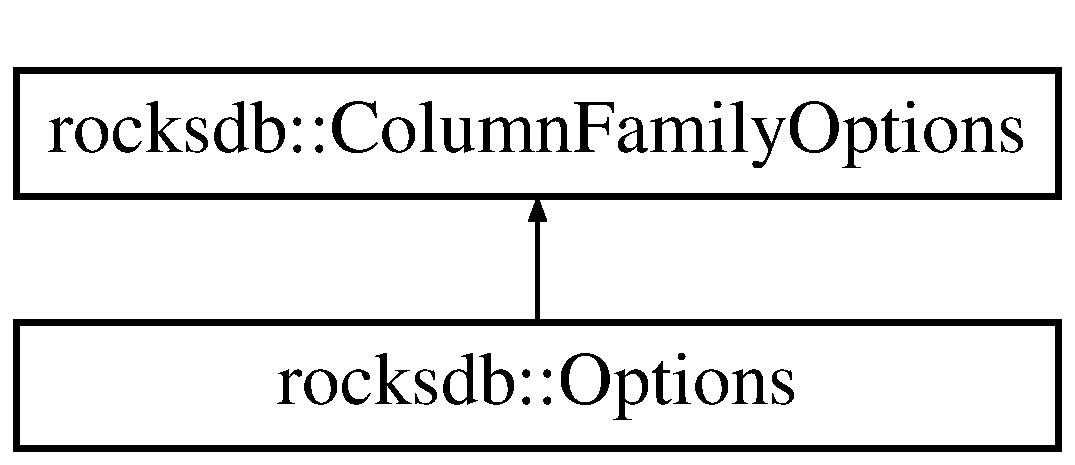
\includegraphics[height=2.000000cm]{structrocksdb_1_1ColumnFamilyOptions}
\end{center}
\end{figure}
\subsection*{Public Types}
\begin{DoxyCompactItemize}
\item 
typedef std\+::vector$<$ std\+::shared\+\_\+ptr$<$ \hyperlink{classrocksdb_1_1TablePropertiesCollectorFactory}{Table\+Properties\+Collector\+Factory} $>$ $>$ {\bfseries Table\+Properties\+Collector\+Factories}\hypertarget{structrocksdb_1_1ColumnFamilyOptions_a1584776ddcea2e26afc9cfa0bf632f6f}{}\label{structrocksdb_1_1ColumnFamilyOptions_a1584776ddcea2e26afc9cfa0bf632f6f}

\end{DoxyCompactItemize}
\subsection*{Public Member Functions}
\begin{DoxyCompactItemize}
\item 
\hyperlink{structrocksdb_1_1ColumnFamilyOptions}{Column\+Family\+Options} $\ast$ {\bfseries Old\+Defaults} (int rocksdb\+\_\+major\+\_\+version=4, int rocksdb\+\_\+minor\+\_\+version=6)\hypertarget{structrocksdb_1_1ColumnFamilyOptions_a7aa3ad0f7ac155931046d0c4bc6a04b6}{}\label{structrocksdb_1_1ColumnFamilyOptions_a7aa3ad0f7ac155931046d0c4bc6a04b6}

\item 
\hyperlink{structrocksdb_1_1ColumnFamilyOptions}{Column\+Family\+Options} $\ast$ {\bfseries Optimize\+For\+Small\+Db} ()\hypertarget{structrocksdb_1_1ColumnFamilyOptions_ad82804c03166c2cca3689daa36da8349}{}\label{structrocksdb_1_1ColumnFamilyOptions_ad82804c03166c2cca3689daa36da8349}

\item 
\hyperlink{structrocksdb_1_1ColumnFamilyOptions}{Column\+Family\+Options} $\ast$ {\bfseries Optimize\+For\+Point\+Lookup} (uint64\+\_\+t block\+\_\+cache\+\_\+size\+\_\+mb)\hypertarget{structrocksdb_1_1ColumnFamilyOptions_aa7608dfefb814f5df10389227f1b0293}{}\label{structrocksdb_1_1ColumnFamilyOptions_aa7608dfefb814f5df10389227f1b0293}

\item 
\hyperlink{structrocksdb_1_1ColumnFamilyOptions}{Column\+Family\+Options} $\ast$ {\bfseries Optimize\+Level\+Style\+Compaction} (uint64\+\_\+t memtable\+\_\+memory\+\_\+budget=512 $\ast$1024 $\ast$1024)\hypertarget{structrocksdb_1_1ColumnFamilyOptions_a4fe010cb8ce0a7accbce36c68c42c7ff}{}\label{structrocksdb_1_1ColumnFamilyOptions_a4fe010cb8ce0a7accbce36c68c42c7ff}

\item 
\hyperlink{structrocksdb_1_1ColumnFamilyOptions}{Column\+Family\+Options} $\ast$ {\bfseries Optimize\+Universal\+Style\+Compaction} (uint64\+\_\+t memtable\+\_\+memory\+\_\+budget=512 $\ast$1024 $\ast$1024)\hypertarget{structrocksdb_1_1ColumnFamilyOptions_a863f08e956f230c203a461a5bd80674e}{}\label{structrocksdb_1_1ColumnFamilyOptions_a863f08e956f230c203a461a5bd80674e}

\item 
{\bfseries Column\+Family\+Options} (const \hyperlink{structrocksdb_1_1Options}{Options} \&options)\hypertarget{structrocksdb_1_1ColumnFamilyOptions_a821f33ce0d7f9a5e5ca9264ca96d4d72}{}\label{structrocksdb_1_1ColumnFamilyOptions_a821f33ce0d7f9a5e5ca9264ca96d4d72}

\item 
void {\bfseries Dump} (\hyperlink{classrocksdb_1_1Logger}{Logger} $\ast$log) const\hypertarget{structrocksdb_1_1ColumnFamilyOptions_ae509bbb7e8710a99d1b8b8443d3ae440}{}\label{structrocksdb_1_1ColumnFamilyOptions_ae509bbb7e8710a99d1b8b8443d3ae440}

\end{DoxyCompactItemize}
\subsection*{Public Attributes}
\begin{DoxyCompactItemize}
\item 
const \hyperlink{classrocksdb_1_1Comparator}{Comparator} $\ast$ {\bfseries comparator}\hypertarget{structrocksdb_1_1ColumnFamilyOptions_adfb6e7d3c9eaa25910a00d5c3f62db4b}{}\label{structrocksdb_1_1ColumnFamilyOptions_adfb6e7d3c9eaa25910a00d5c3f62db4b}

\item 
std\+::shared\+\_\+ptr$<$ \hyperlink{classrocksdb_1_1MergeOperator}{Merge\+Operator} $>$ {\bfseries merge\+\_\+operator}\hypertarget{structrocksdb_1_1ColumnFamilyOptions_ac5b3c36f2f0f1bf0332b96a650747710}{}\label{structrocksdb_1_1ColumnFamilyOptions_ac5b3c36f2f0f1bf0332b96a650747710}

\item 
const \hyperlink{classrocksdb_1_1CompactionFilter}{Compaction\+Filter} $\ast$ {\bfseries compaction\+\_\+filter}\hypertarget{structrocksdb_1_1ColumnFamilyOptions_a8ad6299f938d7e2b1481e156f5caa04c}{}\label{structrocksdb_1_1ColumnFamilyOptions_a8ad6299f938d7e2b1481e156f5caa04c}

\item 
std\+::shared\+\_\+ptr$<$ \hyperlink{classrocksdb_1_1CompactionFilterFactory}{Compaction\+Filter\+Factory} $>$ {\bfseries compaction\+\_\+filter\+\_\+factory}\hypertarget{structrocksdb_1_1ColumnFamilyOptions_a52d9317b197ae0f29dfe5823c593a672}{}\label{structrocksdb_1_1ColumnFamilyOptions_a52d9317b197ae0f29dfe5823c593a672}

\item 
size\+\_\+t {\bfseries write\+\_\+buffer\+\_\+size}\hypertarget{structrocksdb_1_1ColumnFamilyOptions_a0bfb59ff9e6e6636b6bc41cec20c3835}{}\label{structrocksdb_1_1ColumnFamilyOptions_a0bfb59ff9e6e6636b6bc41cec20c3835}

\item 
int {\bfseries max\+\_\+write\+\_\+buffer\+\_\+number}\hypertarget{structrocksdb_1_1ColumnFamilyOptions_aabe9596603e4ce9e9e88ffb6317ebdf1}{}\label{structrocksdb_1_1ColumnFamilyOptions_aabe9596603e4ce9e9e88ffb6317ebdf1}

\item 
int {\bfseries min\+\_\+write\+\_\+buffer\+\_\+number\+\_\+to\+\_\+merge}\hypertarget{structrocksdb_1_1ColumnFamilyOptions_a01a476601097827a39b5d4c938b692b0}{}\label{structrocksdb_1_1ColumnFamilyOptions_a01a476601097827a39b5d4c938b692b0}

\item 
int {\bfseries max\+\_\+write\+\_\+buffer\+\_\+number\+\_\+to\+\_\+maintain}\hypertarget{structrocksdb_1_1ColumnFamilyOptions_a7b01c7716e16303a00378471e3801c49}{}\label{structrocksdb_1_1ColumnFamilyOptions_a7b01c7716e16303a00378471e3801c49}

\item 
Compression\+Type {\bfseries compression}\hypertarget{structrocksdb_1_1ColumnFamilyOptions_a4f1b99a6823346ecf84c3348af150664}{}\label{structrocksdb_1_1ColumnFamilyOptions_a4f1b99a6823346ecf84c3348af150664}

\item 
std\+::vector$<$ Compression\+Type $>$ {\bfseries compression\+\_\+per\+\_\+level}\hypertarget{structrocksdb_1_1ColumnFamilyOptions_a44c7242eb5bf1a2491744100a19a03a4}{}\label{structrocksdb_1_1ColumnFamilyOptions_a44c7242eb5bf1a2491744100a19a03a4}

\item 
\hyperlink{structrocksdb_1_1CompressionOptions}{Compression\+Options} {\bfseries compression\+\_\+opts}\hypertarget{structrocksdb_1_1ColumnFamilyOptions_afeaa71f74b931e03adcdd4d797046649}{}\label{structrocksdb_1_1ColumnFamilyOptions_afeaa71f74b931e03adcdd4d797046649}

\item 
std\+::shared\+\_\+ptr$<$ const \hyperlink{classrocksdb_1_1SliceTransform}{Slice\+Transform} $>$ {\bfseries prefix\+\_\+extractor}\hypertarget{structrocksdb_1_1ColumnFamilyOptions_a0f2502c0d8da4065cb2c17f3bab4ce94}{}\label{structrocksdb_1_1ColumnFamilyOptions_a0f2502c0d8da4065cb2c17f3bab4ce94}

\item 
int {\bfseries num\+\_\+levels}\hypertarget{structrocksdb_1_1ColumnFamilyOptions_a80a36f81f955c2cec0cc5ca5d198a3fb}{}\label{structrocksdb_1_1ColumnFamilyOptions_a80a36f81f955c2cec0cc5ca5d198a3fb}

\item 
int {\bfseries level0\+\_\+file\+\_\+num\+\_\+compaction\+\_\+trigger}\hypertarget{structrocksdb_1_1ColumnFamilyOptions_a32207c8143efa9d6030e7c2fe4bfc5e0}{}\label{structrocksdb_1_1ColumnFamilyOptions_a32207c8143efa9d6030e7c2fe4bfc5e0}

\item 
int {\bfseries level0\+\_\+slowdown\+\_\+writes\+\_\+trigger}\hypertarget{structrocksdb_1_1ColumnFamilyOptions_a215b1a0828086c70f1c6977f50b6c428}{}\label{structrocksdb_1_1ColumnFamilyOptions_a215b1a0828086c70f1c6977f50b6c428}

\item 
int {\bfseries level0\+\_\+stop\+\_\+writes\+\_\+trigger}\hypertarget{structrocksdb_1_1ColumnFamilyOptions_a2e12bced5ac5c71a218c4ed54bc4e869}{}\label{structrocksdb_1_1ColumnFamilyOptions_a2e12bced5ac5c71a218c4ed54bc4e869}

\item 
int {\bfseries max\+\_\+mem\+\_\+compaction\+\_\+level}\hypertarget{structrocksdb_1_1ColumnFamilyOptions_ab34f7e86a0a89ec8afce212064c40e12}{}\label{structrocksdb_1_1ColumnFamilyOptions_ab34f7e86a0a89ec8afce212064c40e12}

\item 
uint64\+\_\+t {\bfseries target\+\_\+file\+\_\+size\+\_\+base}\hypertarget{structrocksdb_1_1ColumnFamilyOptions_a3f7bdb70864f2e4b8c210d741a846ca4}{}\label{structrocksdb_1_1ColumnFamilyOptions_a3f7bdb70864f2e4b8c210d741a846ca4}

\item 
int {\bfseries target\+\_\+file\+\_\+size\+\_\+multiplier}\hypertarget{structrocksdb_1_1ColumnFamilyOptions_a9d29f960f7bf70d74eec3408e5e15d67}{}\label{structrocksdb_1_1ColumnFamilyOptions_a9d29f960f7bf70d74eec3408e5e15d67}

\item 
uint64\+\_\+t {\bfseries max\+\_\+bytes\+\_\+for\+\_\+level\+\_\+base}\hypertarget{structrocksdb_1_1ColumnFamilyOptions_a18bbb667e528c748a6fbd57e402886d8}{}\label{structrocksdb_1_1ColumnFamilyOptions_a18bbb667e528c748a6fbd57e402886d8}

\item 
bool {\bfseries level\+\_\+compaction\+\_\+dynamic\+\_\+level\+\_\+bytes}\hypertarget{structrocksdb_1_1ColumnFamilyOptions_a21d3d9d419bdb9575e5f457a5f976a38}{}\label{structrocksdb_1_1ColumnFamilyOptions_a21d3d9d419bdb9575e5f457a5f976a38}

\item 
int {\bfseries max\+\_\+bytes\+\_\+for\+\_\+level\+\_\+multiplier}\hypertarget{structrocksdb_1_1ColumnFamilyOptions_a4a8ec61f7c6b3b2ff45edd86bc991c00}{}\label{structrocksdb_1_1ColumnFamilyOptions_a4a8ec61f7c6b3b2ff45edd86bc991c00}

\item 
std\+::vector$<$ int $>$ {\bfseries max\+\_\+bytes\+\_\+for\+\_\+level\+\_\+multiplier\+\_\+additional}\hypertarget{structrocksdb_1_1ColumnFamilyOptions_a9cfc4724c3f55e7aeb8d581c4105e82c}{}\label{structrocksdb_1_1ColumnFamilyOptions_a9cfc4724c3f55e7aeb8d581c4105e82c}

\item 
int {\bfseries expanded\+\_\+compaction\+\_\+factor}\hypertarget{structrocksdb_1_1ColumnFamilyOptions_a300d8055fca9135f5fb798ae8ef3e479}{}\label{structrocksdb_1_1ColumnFamilyOptions_a300d8055fca9135f5fb798ae8ef3e479}

\item 
int {\bfseries source\+\_\+compaction\+\_\+factor}\hypertarget{structrocksdb_1_1ColumnFamilyOptions_a8e20e6a60b9057246782c281e10e9b8f}{}\label{structrocksdb_1_1ColumnFamilyOptions_a8e20e6a60b9057246782c281e10e9b8f}

\item 
int {\bfseries max\+\_\+grandparent\+\_\+overlap\+\_\+factor}\hypertarget{structrocksdb_1_1ColumnFamilyOptions_aed9c300c0418ec8feaf441911ce6e42e}{}\label{structrocksdb_1_1ColumnFamilyOptions_aed9c300c0418ec8feaf441911ce6e42e}

\item 
double {\bfseries soft\+\_\+rate\+\_\+limit}\hypertarget{structrocksdb_1_1ColumnFamilyOptions_af45a262b41b58ec6adb82264080edbc9}{}\label{structrocksdb_1_1ColumnFamilyOptions_af45a262b41b58ec6adb82264080edbc9}

\item 
double {\bfseries hard\+\_\+rate\+\_\+limit}\hypertarget{structrocksdb_1_1ColumnFamilyOptions_ad2d0f3ac94f5242fb3cf3e6d5acbcc98}{}\label{structrocksdb_1_1ColumnFamilyOptions_ad2d0f3ac94f5242fb3cf3e6d5acbcc98}

\item 
uint64\+\_\+t {\bfseries soft\+\_\+pending\+\_\+compaction\+\_\+bytes\+\_\+limit}\hypertarget{structrocksdb_1_1ColumnFamilyOptions_a776d5ac1634dcf4b2e2933cb023f859e}{}\label{structrocksdb_1_1ColumnFamilyOptions_a776d5ac1634dcf4b2e2933cb023f859e}

\item 
uint64\+\_\+t {\bfseries hard\+\_\+pending\+\_\+compaction\+\_\+bytes\+\_\+limit}\hypertarget{structrocksdb_1_1ColumnFamilyOptions_a18e4e7ecfdfb50a4b07cd9c3cb92387b}{}\label{structrocksdb_1_1ColumnFamilyOptions_a18e4e7ecfdfb50a4b07cd9c3cb92387b}

\item 
unsigned int {\bfseries rate\+\_\+limit\+\_\+delay\+\_\+max\+\_\+milliseconds}\hypertarget{structrocksdb_1_1ColumnFamilyOptions_af47301838b6ec6a18f9296cf194b5759}{}\label{structrocksdb_1_1ColumnFamilyOptions_af47301838b6ec6a18f9296cf194b5759}

\item 
size\+\_\+t {\bfseries arena\+\_\+block\+\_\+size}\hypertarget{structrocksdb_1_1ColumnFamilyOptions_a5cd888af58cfbcfee795ce460eeb6b90}{}\label{structrocksdb_1_1ColumnFamilyOptions_a5cd888af58cfbcfee795ce460eeb6b90}

\item 
bool {\bfseries disable\+\_\+auto\+\_\+compactions}\hypertarget{structrocksdb_1_1ColumnFamilyOptions_a7bf2bd83902d9daa690a1573c9d20523}{}\label{structrocksdb_1_1ColumnFamilyOptions_a7bf2bd83902d9daa690a1573c9d20523}

\item 
bool {\bfseries purge\+\_\+redundant\+\_\+kvs\+\_\+while\+\_\+flush}\hypertarget{structrocksdb_1_1ColumnFamilyOptions_ad2a4d376117a9caa7d25b3aa15c9d7b9}{}\label{structrocksdb_1_1ColumnFamilyOptions_ad2a4d376117a9caa7d25b3aa15c9d7b9}

\item 
Compaction\+Style {\bfseries compaction\+\_\+style}\hypertarget{structrocksdb_1_1ColumnFamilyOptions_af23f2504801df411a8ba336743bc3481}{}\label{structrocksdb_1_1ColumnFamilyOptions_af23f2504801df411a8ba336743bc3481}

\item 
Compaction\+Pri {\bfseries compaction\+\_\+pri}\hypertarget{structrocksdb_1_1ColumnFamilyOptions_a0795b8f337f5a63fd9666648202a02e3}{}\label{structrocksdb_1_1ColumnFamilyOptions_a0795b8f337f5a63fd9666648202a02e3}

\item 
bool {\bfseries verify\+\_\+checksums\+\_\+in\+\_\+compaction}\hypertarget{structrocksdb_1_1ColumnFamilyOptions_a467caa4ed08291dccd0e378edfaf99ab}{}\label{structrocksdb_1_1ColumnFamilyOptions_a467caa4ed08291dccd0e378edfaf99ab}

\item 
\hyperlink{classrocksdb_1_1CompactionOptionsUniversal}{Compaction\+Options\+Universal} {\bfseries compaction\+\_\+options\+\_\+universal}\hypertarget{structrocksdb_1_1ColumnFamilyOptions_a487e37a1e34823d87fc24d0fbd03ee46}{}\label{structrocksdb_1_1ColumnFamilyOptions_a487e37a1e34823d87fc24d0fbd03ee46}

\item 
\hyperlink{structrocksdb_1_1CompactionOptionsFIFO}{Compaction\+Options\+F\+I\+FO} {\bfseries compaction\+\_\+options\+\_\+fifo}\hypertarget{structrocksdb_1_1ColumnFamilyOptions_ac9c65f6f6da764046ce6b1f69d68526d}{}\label{structrocksdb_1_1ColumnFamilyOptions_ac9c65f6f6da764046ce6b1f69d68526d}

\item 
bool {\bfseries filter\+\_\+deletes}\hypertarget{structrocksdb_1_1ColumnFamilyOptions_a8fc54e6814cf87a7cc138e03f165376a}{}\label{structrocksdb_1_1ColumnFamilyOptions_a8fc54e6814cf87a7cc138e03f165376a}

\item 
uint64\+\_\+t {\bfseries max\+\_\+sequential\+\_\+skip\+\_\+in\+\_\+iterations}\hypertarget{structrocksdb_1_1ColumnFamilyOptions_a5a584b6d8a12d67a6a518b72772314a0}{}\label{structrocksdb_1_1ColumnFamilyOptions_a5a584b6d8a12d67a6a518b72772314a0}

\item 
std\+::shared\+\_\+ptr$<$ \hyperlink{classrocksdb_1_1MemTableRepFactory}{Mem\+Table\+Rep\+Factory} $>$ {\bfseries memtable\+\_\+factory}\hypertarget{structrocksdb_1_1ColumnFamilyOptions_a9b3cc4ef5a3a18b5ca655562c13a8124}{}\label{structrocksdb_1_1ColumnFamilyOptions_a9b3cc4ef5a3a18b5ca655562c13a8124}

\item 
std\+::shared\+\_\+ptr$<$ \hyperlink{classrocksdb_1_1TableFactory}{Table\+Factory} $>$ {\bfseries table\+\_\+factory}\hypertarget{structrocksdb_1_1ColumnFamilyOptions_a70c618eb7f362c5369e834447f8500de}{}\label{structrocksdb_1_1ColumnFamilyOptions_a70c618eb7f362c5369e834447f8500de}

\item 
Table\+Properties\+Collector\+Factories {\bfseries table\+\_\+properties\+\_\+collector\+\_\+factories}\hypertarget{structrocksdb_1_1ColumnFamilyOptions_ad4481d12bf82c5958b8095d7bd0b65e0}{}\label{structrocksdb_1_1ColumnFamilyOptions_ad4481d12bf82c5958b8095d7bd0b65e0}

\item 
bool {\bfseries inplace\+\_\+update\+\_\+support}\hypertarget{structrocksdb_1_1ColumnFamilyOptions_a9c26b13c7b636589ad7593d4b58f65ce}{}\label{structrocksdb_1_1ColumnFamilyOptions_a9c26b13c7b636589ad7593d4b58f65ce}

\item 
size\+\_\+t {\bfseries inplace\+\_\+update\+\_\+num\+\_\+locks}\hypertarget{structrocksdb_1_1ColumnFamilyOptions_a9e7478e72e22fdbaead1fea0c9baee3e}{}\label{structrocksdb_1_1ColumnFamilyOptions_a9e7478e72e22fdbaead1fea0c9baee3e}

\item 
Update\+Status($\ast$ {\bfseries inplace\+\_\+callback} )(char $\ast$existing\+\_\+value, uint32\+\_\+t $\ast$existing\+\_\+value\+\_\+size, \hyperlink{classrocksdb_1_1Slice}{Slice} delta\+\_\+value, std\+::string $\ast$merged\+\_\+value)\hypertarget{structrocksdb_1_1ColumnFamilyOptions_afdc856c10d5fc60f6bb2de0d5ebe14bf}{}\label{structrocksdb_1_1ColumnFamilyOptions_afdc856c10d5fc60f6bb2de0d5ebe14bf}

\item 
uint32\+\_\+t {\bfseries memtable\+\_\+prefix\+\_\+bloom\+\_\+bits}\hypertarget{structrocksdb_1_1ColumnFamilyOptions_a2948f1db5ec9c129c30cf53b89e6a4fb}{}\label{structrocksdb_1_1ColumnFamilyOptions_a2948f1db5ec9c129c30cf53b89e6a4fb}

\item 
uint32\+\_\+t {\bfseries memtable\+\_\+prefix\+\_\+bloom\+\_\+probes}\hypertarget{structrocksdb_1_1ColumnFamilyOptions_a2ec3c3476d17cd09df406503af29c541}{}\label{structrocksdb_1_1ColumnFamilyOptions_a2ec3c3476d17cd09df406503af29c541}

\item 
size\+\_\+t {\bfseries memtable\+\_\+prefix\+\_\+bloom\+\_\+huge\+\_\+page\+\_\+tlb\+\_\+size}\hypertarget{structrocksdb_1_1ColumnFamilyOptions_a5a486f891b1a6e1c160423a4ca1cf614}{}\label{structrocksdb_1_1ColumnFamilyOptions_a5a486f891b1a6e1c160423a4ca1cf614}

\item 
uint32\+\_\+t {\bfseries bloom\+\_\+locality}\hypertarget{structrocksdb_1_1ColumnFamilyOptions_ade1810e42d9976ad7c3b04deaedecb8c}{}\label{structrocksdb_1_1ColumnFamilyOptions_ade1810e42d9976ad7c3b04deaedecb8c}

\item 
size\+\_\+t {\bfseries max\+\_\+successive\+\_\+merges}\hypertarget{structrocksdb_1_1ColumnFamilyOptions_a859ff3de043df6b3c56fb3864059af97}{}\label{structrocksdb_1_1ColumnFamilyOptions_a859ff3de043df6b3c56fb3864059af97}

\item 
uint32\+\_\+t {\bfseries min\+\_\+partial\+\_\+merge\+\_\+operands}\hypertarget{structrocksdb_1_1ColumnFamilyOptions_aa4ab70aa69ead877276ed0bdd3dcdd57}{}\label{structrocksdb_1_1ColumnFamilyOptions_aa4ab70aa69ead877276ed0bdd3dcdd57}

\item 
bool {\bfseries optimize\+\_\+filters\+\_\+for\+\_\+hits}\hypertarget{structrocksdb_1_1ColumnFamilyOptions_a76c648dd39b9abbb4f6cade7622feba2}{}\label{structrocksdb_1_1ColumnFamilyOptions_a76c648dd39b9abbb4f6cade7622feba2}

\item 
bool {\bfseries paranoid\+\_\+file\+\_\+checks}\hypertarget{structrocksdb_1_1ColumnFamilyOptions_a2467b8c33a910ab2a52a30040e3f1658}{}\label{structrocksdb_1_1ColumnFamilyOptions_a2467b8c33a910ab2a52a30040e3f1658}

\item 
bool {\bfseries compaction\+\_\+measure\+\_\+io\+\_\+stats}\hypertarget{structrocksdb_1_1ColumnFamilyOptions_a4464c82cabd9e13f26ca8551006988a5}{}\label{structrocksdb_1_1ColumnFamilyOptions_a4464c82cabd9e13f26ca8551006988a5}

\end{DoxyCompactItemize}


The documentation for this struct was generated from the following file\+:\begin{DoxyCompactItemize}
\item 
Appserver/src/external/rocksdb/options.\+h\end{DoxyCompactItemize}

\hypertarget{structJson_1_1CommentStyle}{}\section{Json\+:\+:Comment\+Style Struct Reference}
\label{structJson_1_1CommentStyle}\index{Json\+::\+Comment\+Style@{Json\+::\+Comment\+Style}}


Scoped enums are not available until C++11.  


\subsection*{Public Types}
\begin{DoxyCompactItemize}
\item 
enum \hyperlink{structJson_1_1CommentStyle_a51fc08f3518fd81eba12f340d19a3d0c}{Enum} \{ \hyperlink{structJson_1_1CommentStyle_a51fc08f3518fd81eba12f340d19a3d0cac8b32a8bae63414c8647d4919da8d437}{None}, 
\hyperlink{structJson_1_1CommentStyle_a51fc08f3518fd81eba12f340d19a3d0cac65238f050773c107690a456e9c05c98}{Most}, 
\hyperlink{structJson_1_1CommentStyle_a51fc08f3518fd81eba12f340d19a3d0ca32302c0b97190c1808b3e38f367fef01}{All}
 \}\begin{DoxyCompactList}\small\item\em Decide whether to write comments. \end{DoxyCompactList}
\end{DoxyCompactItemize}


\subsection{Detailed Description}
Scoped enums are not available until C++11. 

\subsection{Member Enumeration Documentation}
\index{Json\+::\+Comment\+Style@{Json\+::\+Comment\+Style}!Enum@{Enum}}
\index{Enum@{Enum}!Json\+::\+Comment\+Style@{Json\+::\+Comment\+Style}}
\subsubsection[{\texorpdfstring{Enum}{Enum}}]{\setlength{\rightskip}{0pt plus 5cm}enum {\bf Json\+::\+Comment\+Style\+::\+Enum}}\hypertarget{structJson_1_1CommentStyle_a51fc08f3518fd81eba12f340d19a3d0c}{}\label{structJson_1_1CommentStyle_a51fc08f3518fd81eba12f340d19a3d0c}


Decide whether to write comments. 

\begin{Desc}
\item[Enumerator]\par
\begin{description}
\index{None@{None}!Json\+::\+Comment\+Style@{Json\+::\+Comment\+Style}}\index{Json\+::\+Comment\+Style@{Json\+::\+Comment\+Style}!None@{None}}\item[{\em 
None\hypertarget{structJson_1_1CommentStyle_a51fc08f3518fd81eba12f340d19a3d0cac8b32a8bae63414c8647d4919da8d437}{}\label{structJson_1_1CommentStyle_a51fc08f3518fd81eba12f340d19a3d0cac8b32a8bae63414c8647d4919da8d437}
}]Drop all comments. \index{Most@{Most}!Json\+::\+Comment\+Style@{Json\+::\+Comment\+Style}}\index{Json\+::\+Comment\+Style@{Json\+::\+Comment\+Style}!Most@{Most}}\item[{\em 
Most\hypertarget{structJson_1_1CommentStyle_a51fc08f3518fd81eba12f340d19a3d0cac65238f050773c107690a456e9c05c98}{}\label{structJson_1_1CommentStyle_a51fc08f3518fd81eba12f340d19a3d0cac65238f050773c107690a456e9c05c98}
}]Recover odd behavior of previous versions (not implemented yet). \index{All@{All}!Json\+::\+Comment\+Style@{Json\+::\+Comment\+Style}}\index{Json\+::\+Comment\+Style@{Json\+::\+Comment\+Style}!All@{All}}\item[{\em 
All\hypertarget{structJson_1_1CommentStyle_a51fc08f3518fd81eba12f340d19a3d0ca32302c0b97190c1808b3e38f367fef01}{}\label{structJson_1_1CommentStyle_a51fc08f3518fd81eba12f340d19a3d0ca32302c0b97190c1808b3e38f367fef01}
}]Keep all comments. \end{description}
\end{Desc}


The documentation for this struct was generated from the following file\+:\begin{DoxyCompactItemize}
\item 
Appserver/src/external/json/jsoncpp.\+cpp\end{DoxyCompactItemize}

\hypertarget{classrocksdb_1_1CompactionFilter}{}\section{rocksdb\+:\+:Compaction\+Filter Class Reference}
\label{classrocksdb_1_1CompactionFilter}\index{rocksdb\+::\+Compaction\+Filter@{rocksdb\+::\+Compaction\+Filter}}
\subsection*{Classes}
\begin{DoxyCompactItemize}
\item 
struct \hyperlink{structrocksdb_1_1CompactionFilter_1_1Context}{Context}
\end{DoxyCompactItemize}
\subsection*{Public Member Functions}
\begin{DoxyCompactItemize}
\item 
virtual bool {\bfseries Filter} (int level, const \hyperlink{classrocksdb_1_1Slice}{Slice} \&key, const \hyperlink{classrocksdb_1_1Slice}{Slice} \&existing\+\_\+value, std\+::string $\ast$new\+\_\+value, bool $\ast$value\+\_\+changed) const =0\hypertarget{classrocksdb_1_1CompactionFilter_a7895ef194328ca68419f4559f8ef3f3e}{}\label{classrocksdb_1_1CompactionFilter_a7895ef194328ca68419f4559f8ef3f3e}

\item 
virtual bool {\bfseries Filter\+Merge\+Operand} (int level, const \hyperlink{classrocksdb_1_1Slice}{Slice} \&key, const \hyperlink{classrocksdb_1_1Slice}{Slice} \&operand) const\hypertarget{classrocksdb_1_1CompactionFilter_abbb7b97125949575155147d0ed3c0349}{}\label{classrocksdb_1_1CompactionFilter_abbb7b97125949575155147d0ed3c0349}

\item 
virtual bool {\bfseries Ignore\+Snapshots} () const\hypertarget{classrocksdb_1_1CompactionFilter_ac441dd2c4d04235b47b2367c821cb36c}{}\label{classrocksdb_1_1CompactionFilter_ac441dd2c4d04235b47b2367c821cb36c}

\item 
virtual const char $\ast$ {\bfseries Name} () const =0\hypertarget{classrocksdb_1_1CompactionFilter_ad1494025487cde909a53510b94456d56}{}\label{classrocksdb_1_1CompactionFilter_ad1494025487cde909a53510b94456d56}

\end{DoxyCompactItemize}


The documentation for this class was generated from the following file\+:\begin{DoxyCompactItemize}
\item 
Appserver/src/external/rocksdb/compaction\+\_\+filter.\+h\end{DoxyCompactItemize}

\hypertarget{structrocksdb_1_1CompactionFilterContext}{}\section{rocksdb\+:\+:Compaction\+Filter\+Context Struct Reference}
\label{structrocksdb_1_1CompactionFilterContext}\index{rocksdb\+::\+Compaction\+Filter\+Context@{rocksdb\+::\+Compaction\+Filter\+Context}}
\subsection*{Public Attributes}
\begin{DoxyCompactItemize}
\item 
bool {\bfseries is\+\_\+full\+\_\+compaction}\hypertarget{structrocksdb_1_1CompactionFilterContext_a20d92a989834e163b7b1ecac1490ce6a}{}\label{structrocksdb_1_1CompactionFilterContext_a20d92a989834e163b7b1ecac1490ce6a}

\item 
bool {\bfseries is\+\_\+manual\+\_\+compaction}\hypertarget{structrocksdb_1_1CompactionFilterContext_a6085fdf0527b0ddb1b851240f47c7f16}{}\label{structrocksdb_1_1CompactionFilterContext_a6085fdf0527b0ddb1b851240f47c7f16}

\end{DoxyCompactItemize}


The documentation for this struct was generated from the following file\+:\begin{DoxyCompactItemize}
\item 
Appserver/src/external/rocksdb/compaction\+\_\+filter.\+h\end{DoxyCompactItemize}

\hypertarget{classrocksdb_1_1CompactionFilterFactory}{}\section{rocksdb\+:\+:Compaction\+Filter\+Factory Class Reference}
\label{classrocksdb_1_1CompactionFilterFactory}\index{rocksdb\+::\+Compaction\+Filter\+Factory@{rocksdb\+::\+Compaction\+Filter\+Factory}}
\subsection*{Public Member Functions}
\begin{DoxyCompactItemize}
\item 
virtual std\+::unique\+\_\+ptr$<$ \hyperlink{classrocksdb_1_1CompactionFilter}{Compaction\+Filter} $>$ {\bfseries Create\+Compaction\+Filter} (const \hyperlink{structrocksdb_1_1CompactionFilter_1_1Context}{Compaction\+Filter\+::\+Context} \&context)=0\hypertarget{classrocksdb_1_1CompactionFilterFactory_aa10d1e526d33243a49ad98243d442ea1}{}\label{classrocksdb_1_1CompactionFilterFactory_aa10d1e526d33243a49ad98243d442ea1}

\item 
virtual const char $\ast$ {\bfseries Name} () const =0\hypertarget{classrocksdb_1_1CompactionFilterFactory_a83ee8a6459e6c2d6806f6221b834a750}{}\label{classrocksdb_1_1CompactionFilterFactory_a83ee8a6459e6c2d6806f6221b834a750}

\end{DoxyCompactItemize}


The documentation for this class was generated from the following file\+:\begin{DoxyCompactItemize}
\item 
Appserver/src/external/rocksdb/compaction\+\_\+filter.\+h\end{DoxyCompactItemize}

\hypertarget{structrocksdb_1_1CompactionJobInfo}{}\section{rocksdb\+:\+:Compaction\+Job\+Info Struct Reference}
\label{structrocksdb_1_1CompactionJobInfo}\index{rocksdb\+::\+Compaction\+Job\+Info@{rocksdb\+::\+Compaction\+Job\+Info}}
\subsection*{Public Member Functions}
\begin{DoxyCompactItemize}
\item 
{\bfseries Compaction\+Job\+Info} (const \hyperlink{structrocksdb_1_1CompactionJobStats}{Compaction\+Job\+Stats} \&\+\_\+stats)\hypertarget{structrocksdb_1_1CompactionJobInfo_a8d54f1c4b1aee7a12c32fd7beab9f1ef}{}\label{structrocksdb_1_1CompactionJobInfo_a8d54f1c4b1aee7a12c32fd7beab9f1ef}

\end{DoxyCompactItemize}
\subsection*{Public Attributes}
\begin{DoxyCompactItemize}
\item 
std\+::string {\bfseries cf\+\_\+name}\hypertarget{structrocksdb_1_1CompactionJobInfo_aacbd3037dd53ade1bd7bca97e8268e39}{}\label{structrocksdb_1_1CompactionJobInfo_aacbd3037dd53ade1bd7bca97e8268e39}

\item 
\hyperlink{classrocksdb_1_1Status}{Status} {\bfseries status}\hypertarget{structrocksdb_1_1CompactionJobInfo_a53eaaa3b53c9bf62b84d86d3c0a02399}{}\label{structrocksdb_1_1CompactionJobInfo_a53eaaa3b53c9bf62b84d86d3c0a02399}

\item 
uint64\+\_\+t {\bfseries thread\+\_\+id}\hypertarget{structrocksdb_1_1CompactionJobInfo_a833d35256c54be979199c1af036f8f6d}{}\label{structrocksdb_1_1CompactionJobInfo_a833d35256c54be979199c1af036f8f6d}

\item 
int {\bfseries job\+\_\+id}\hypertarget{structrocksdb_1_1CompactionJobInfo_ad5eb897de9c40c55dd7011d4ed4c0096}{}\label{structrocksdb_1_1CompactionJobInfo_ad5eb897de9c40c55dd7011d4ed4c0096}

\item 
int {\bfseries base\+\_\+input\+\_\+level}\hypertarget{structrocksdb_1_1CompactionJobInfo_a5e023143a01c181a17dbd3b80181fba5}{}\label{structrocksdb_1_1CompactionJobInfo_a5e023143a01c181a17dbd3b80181fba5}

\item 
int {\bfseries output\+\_\+level}\hypertarget{structrocksdb_1_1CompactionJobInfo_af018098d27ea7a3ec51850973510c253}{}\label{structrocksdb_1_1CompactionJobInfo_af018098d27ea7a3ec51850973510c253}

\item 
std\+::vector$<$ std\+::string $>$ {\bfseries input\+\_\+files}\hypertarget{structrocksdb_1_1CompactionJobInfo_a159303c2316a367d7f55dc09fe255f25}{}\label{structrocksdb_1_1CompactionJobInfo_a159303c2316a367d7f55dc09fe255f25}

\item 
std\+::vector$<$ std\+::string $>$ {\bfseries output\+\_\+files}\hypertarget{structrocksdb_1_1CompactionJobInfo_a0cf1e4c7357345baefbf384555692846}{}\label{structrocksdb_1_1CompactionJobInfo_a0cf1e4c7357345baefbf384555692846}

\item 
Table\+Properties\+Collection {\bfseries table\+\_\+properties}\hypertarget{structrocksdb_1_1CompactionJobInfo_ad2afb3bdbf47e8a94a646bc51500f800}{}\label{structrocksdb_1_1CompactionJobInfo_ad2afb3bdbf47e8a94a646bc51500f800}

\item 
Compaction\+Reason {\bfseries compaction\+\_\+reason}\hypertarget{structrocksdb_1_1CompactionJobInfo_a55ed52084f36f0456a21794c2d9ba547}{}\label{structrocksdb_1_1CompactionJobInfo_a55ed52084f36f0456a21794c2d9ba547}

\item 
\hyperlink{structrocksdb_1_1CompactionJobStats}{Compaction\+Job\+Stats} {\bfseries stats}\hypertarget{structrocksdb_1_1CompactionJobInfo_a393e4d0075f482bdcca653e308a67f64}{}\label{structrocksdb_1_1CompactionJobInfo_a393e4d0075f482bdcca653e308a67f64}

\end{DoxyCompactItemize}


The documentation for this struct was generated from the following file\+:\begin{DoxyCompactItemize}
\item 
Appserver/src/external/rocksdb/listener.\+h\end{DoxyCompactItemize}

\hypertarget{structrocksdb_1_1CompactionJobStats}{}\section{rocksdb\+:\+:Compaction\+Job\+Stats Struct Reference}
\label{structrocksdb_1_1CompactionJobStats}\index{rocksdb\+::\+Compaction\+Job\+Stats@{rocksdb\+::\+Compaction\+Job\+Stats}}
\subsection*{Public Member Functions}
\begin{DoxyCompactItemize}
\item 
void {\bfseries Reset} ()\hypertarget{structrocksdb_1_1CompactionJobStats_af0195248906328fd3b8f27d55ae9425f}{}\label{structrocksdb_1_1CompactionJobStats_af0195248906328fd3b8f27d55ae9425f}

\item 
void {\bfseries Add} (const \hyperlink{structrocksdb_1_1CompactionJobStats}{Compaction\+Job\+Stats} \&stats)\hypertarget{structrocksdb_1_1CompactionJobStats_a3bc84f5f31d8281195c68255bc75cfc3}{}\label{structrocksdb_1_1CompactionJobStats_a3bc84f5f31d8281195c68255bc75cfc3}

\end{DoxyCompactItemize}
\subsection*{Public Attributes}
\begin{DoxyCompactItemize}
\item 
uint64\+\_\+t {\bfseries elapsed\+\_\+micros}\hypertarget{structrocksdb_1_1CompactionJobStats_a6567d468a65804786f63cc4479be6c6f}{}\label{structrocksdb_1_1CompactionJobStats_a6567d468a65804786f63cc4479be6c6f}

\item 
uint64\+\_\+t {\bfseries num\+\_\+input\+\_\+records}\hypertarget{structrocksdb_1_1CompactionJobStats_aa59a71837c8db2b6d3fbd619d9abfa97}{}\label{structrocksdb_1_1CompactionJobStats_aa59a71837c8db2b6d3fbd619d9abfa97}

\item 
size\+\_\+t {\bfseries num\+\_\+input\+\_\+files}\hypertarget{structrocksdb_1_1CompactionJobStats_ad51b1dbb1097f47965e03a1f0df1dae0}{}\label{structrocksdb_1_1CompactionJobStats_ad51b1dbb1097f47965e03a1f0df1dae0}

\item 
size\+\_\+t {\bfseries num\+\_\+input\+\_\+files\+\_\+at\+\_\+output\+\_\+level}\hypertarget{structrocksdb_1_1CompactionJobStats_a4bd332cb2fd690781e28b45340819511}{}\label{structrocksdb_1_1CompactionJobStats_a4bd332cb2fd690781e28b45340819511}

\item 
uint64\+\_\+t {\bfseries num\+\_\+output\+\_\+records}\hypertarget{structrocksdb_1_1CompactionJobStats_a23be31caaba0bc26d62329f2d9b9da82}{}\label{structrocksdb_1_1CompactionJobStats_a23be31caaba0bc26d62329f2d9b9da82}

\item 
size\+\_\+t {\bfseries num\+\_\+output\+\_\+files}\hypertarget{structrocksdb_1_1CompactionJobStats_a28cb3dcc37534dc043e75a5218f12243}{}\label{structrocksdb_1_1CompactionJobStats_a28cb3dcc37534dc043e75a5218f12243}

\item 
bool {\bfseries is\+\_\+manual\+\_\+compaction}\hypertarget{structrocksdb_1_1CompactionJobStats_ae07cc8e438bcafbfd3fe9899dd323dde}{}\label{structrocksdb_1_1CompactionJobStats_ae07cc8e438bcafbfd3fe9899dd323dde}

\item 
uint64\+\_\+t {\bfseries total\+\_\+input\+\_\+bytes}\hypertarget{structrocksdb_1_1CompactionJobStats_a097802ababbd8561713ebdd013af291b}{}\label{structrocksdb_1_1CompactionJobStats_a097802ababbd8561713ebdd013af291b}

\item 
uint64\+\_\+t {\bfseries total\+\_\+output\+\_\+bytes}\hypertarget{structrocksdb_1_1CompactionJobStats_adf968cd75deab45d379fa203899ce5fb}{}\label{structrocksdb_1_1CompactionJobStats_adf968cd75deab45d379fa203899ce5fb}

\item 
uint64\+\_\+t {\bfseries num\+\_\+records\+\_\+replaced}\hypertarget{structrocksdb_1_1CompactionJobStats_a1c79e44c92dd9faa6888ca26937a210a}{}\label{structrocksdb_1_1CompactionJobStats_a1c79e44c92dd9faa6888ca26937a210a}

\item 
uint64\+\_\+t {\bfseries total\+\_\+input\+\_\+raw\+\_\+key\+\_\+bytes}\hypertarget{structrocksdb_1_1CompactionJobStats_a910330008a971df31761388ab43938cb}{}\label{structrocksdb_1_1CompactionJobStats_a910330008a971df31761388ab43938cb}

\item 
uint64\+\_\+t {\bfseries total\+\_\+input\+\_\+raw\+\_\+value\+\_\+bytes}\hypertarget{structrocksdb_1_1CompactionJobStats_a8a1a5bb5fba130c88f22fcc8dbbf33d4}{}\label{structrocksdb_1_1CompactionJobStats_a8a1a5bb5fba130c88f22fcc8dbbf33d4}

\item 
uint64\+\_\+t {\bfseries num\+\_\+input\+\_\+deletion\+\_\+records}\hypertarget{structrocksdb_1_1CompactionJobStats_a26690d30147da530ccb58b31664bd842}{}\label{structrocksdb_1_1CompactionJobStats_a26690d30147da530ccb58b31664bd842}

\item 
uint64\+\_\+t {\bfseries num\+\_\+expired\+\_\+deletion\+\_\+records}\hypertarget{structrocksdb_1_1CompactionJobStats_a93fa71d4acdde55345a0dfd341525d68}{}\label{structrocksdb_1_1CompactionJobStats_a93fa71d4acdde55345a0dfd341525d68}

\item 
uint64\+\_\+t {\bfseries num\+\_\+corrupt\+\_\+keys}\hypertarget{structrocksdb_1_1CompactionJobStats_acd7628e417f48a0f7eab1e1732c6c27d}{}\label{structrocksdb_1_1CompactionJobStats_acd7628e417f48a0f7eab1e1732c6c27d}

\item 
uint64\+\_\+t {\bfseries file\+\_\+write\+\_\+nanos}\hypertarget{structrocksdb_1_1CompactionJobStats_a442fa7d03821f9c107dfac2bb049f9b5}{}\label{structrocksdb_1_1CompactionJobStats_a442fa7d03821f9c107dfac2bb049f9b5}

\item 
uint64\+\_\+t {\bfseries file\+\_\+range\+\_\+sync\+\_\+nanos}\hypertarget{structrocksdb_1_1CompactionJobStats_af3b2635781a0ac9ad2e9e2eb6b01dcfc}{}\label{structrocksdb_1_1CompactionJobStats_af3b2635781a0ac9ad2e9e2eb6b01dcfc}

\item 
uint64\+\_\+t {\bfseries file\+\_\+fsync\+\_\+nanos}\hypertarget{structrocksdb_1_1CompactionJobStats_ae9faea0656e11b736aeac6d35facc700}{}\label{structrocksdb_1_1CompactionJobStats_ae9faea0656e11b736aeac6d35facc700}

\item 
uint64\+\_\+t {\bfseries file\+\_\+prepare\+\_\+write\+\_\+nanos}\hypertarget{structrocksdb_1_1CompactionJobStats_a5cf8dcee3c51604d9a45fd221fab792a}{}\label{structrocksdb_1_1CompactionJobStats_a5cf8dcee3c51604d9a45fd221fab792a}

\item 
std\+::string {\bfseries smallest\+\_\+output\+\_\+key\+\_\+prefix}\hypertarget{structrocksdb_1_1CompactionJobStats_a566d94f35ffb42149030263118c51819}{}\label{structrocksdb_1_1CompactionJobStats_a566d94f35ffb42149030263118c51819}

\item 
std\+::string {\bfseries largest\+\_\+output\+\_\+key\+\_\+prefix}\hypertarget{structrocksdb_1_1CompactionJobStats_adcb6ac0e33c7eafd46999a2d152b018d}{}\label{structrocksdb_1_1CompactionJobStats_adcb6ac0e33c7eafd46999a2d152b018d}

\end{DoxyCompactItemize}
\subsection*{Static Public Attributes}
\begin{DoxyCompactItemize}
\item 
static const size\+\_\+t {\bfseries k\+Max\+Prefix\+Length} = 8\hypertarget{structrocksdb_1_1CompactionJobStats_a6cb8682c28a6fff939bc793d407fac95}{}\label{structrocksdb_1_1CompactionJobStats_a6cb8682c28a6fff939bc793d407fac95}

\end{DoxyCompactItemize}


The documentation for this struct was generated from the following file\+:\begin{DoxyCompactItemize}
\item 
Appserver/src/external/rocksdb/compaction\+\_\+job\+\_\+stats.\+h\end{DoxyCompactItemize}

\hypertarget{structrocksdb_1_1CompactionOptions}{}\section{rocksdb\+:\+:Compaction\+Options Struct Reference}
\label{structrocksdb_1_1CompactionOptions}\index{rocksdb\+::\+Compaction\+Options@{rocksdb\+::\+Compaction\+Options}}
\subsection*{Public Attributes}
\begin{DoxyCompactItemize}
\item 
Compression\+Type {\bfseries compression}\hypertarget{structrocksdb_1_1CompactionOptions_a315a9f172bf163fec933dc51ba53df7f}{}\label{structrocksdb_1_1CompactionOptions_a315a9f172bf163fec933dc51ba53df7f}

\item 
uint64\+\_\+t {\bfseries output\+\_\+file\+\_\+size\+\_\+limit}\hypertarget{structrocksdb_1_1CompactionOptions_a6dc9c8d555444cda47fee94d520c4a1a}{}\label{structrocksdb_1_1CompactionOptions_a6dc9c8d555444cda47fee94d520c4a1a}

\end{DoxyCompactItemize}


The documentation for this struct was generated from the following file\+:\begin{DoxyCompactItemize}
\item 
Appserver/src/external/rocksdb/options.\+h\end{DoxyCompactItemize}

\hypertarget{structrocksdb_1_1CompactionOptionsFIFO}{}\section{rocksdb\+:\+:Compaction\+Options\+F\+I\+FO Struct Reference}
\label{structrocksdb_1_1CompactionOptionsFIFO}\index{rocksdb\+::\+Compaction\+Options\+F\+I\+FO@{rocksdb\+::\+Compaction\+Options\+F\+I\+FO}}
\subsection*{Public Attributes}
\begin{DoxyCompactItemize}
\item 
uint64\+\_\+t {\bfseries max\+\_\+table\+\_\+files\+\_\+size}\hypertarget{structrocksdb_1_1CompactionOptionsFIFO_a54a997cb1d9a8d3b7eb2b6edbf5ccf42}{}\label{structrocksdb_1_1CompactionOptionsFIFO_a54a997cb1d9a8d3b7eb2b6edbf5ccf42}

\end{DoxyCompactItemize}


The documentation for this struct was generated from the following file\+:\begin{DoxyCompactItemize}
\item 
Appserver/src/external/rocksdb/options.\+h\end{DoxyCompactItemize}

\hypertarget{classrocksdb_1_1CompactionOptionsUniversal}{}\section{rocksdb\+:\+:Compaction\+Options\+Universal Class Reference}
\label{classrocksdb_1_1CompactionOptionsUniversal}\index{rocksdb\+::\+Compaction\+Options\+Universal@{rocksdb\+::\+Compaction\+Options\+Universal}}
\subsection*{Public Attributes}
\begin{DoxyCompactItemize}
\item 
unsigned int {\bfseries size\+\_\+ratio}\hypertarget{classrocksdb_1_1CompactionOptionsUniversal_afe1e4100c1ce559c539b020ec7b46361}{}\label{classrocksdb_1_1CompactionOptionsUniversal_afe1e4100c1ce559c539b020ec7b46361}

\item 
unsigned int {\bfseries min\+\_\+merge\+\_\+width}\hypertarget{classrocksdb_1_1CompactionOptionsUniversal_a2e0a22409db14dedca88773e9c47e778}{}\label{classrocksdb_1_1CompactionOptionsUniversal_a2e0a22409db14dedca88773e9c47e778}

\item 
unsigned int {\bfseries max\+\_\+merge\+\_\+width}\hypertarget{classrocksdb_1_1CompactionOptionsUniversal_af30ea01da6c70b626b955f6df59f33a1}{}\label{classrocksdb_1_1CompactionOptionsUniversal_af30ea01da6c70b626b955f6df59f33a1}

\item 
unsigned int {\bfseries max\+\_\+size\+\_\+amplification\+\_\+percent}\hypertarget{classrocksdb_1_1CompactionOptionsUniversal_a4ac3f2dc4ee2552b49607c5b70b706ce}{}\label{classrocksdb_1_1CompactionOptionsUniversal_a4ac3f2dc4ee2552b49607c5b70b706ce}

\item 
int {\bfseries compression\+\_\+size\+\_\+percent}\hypertarget{classrocksdb_1_1CompactionOptionsUniversal_afcd15128bac78da1023eff339c63d015}{}\label{classrocksdb_1_1CompactionOptionsUniversal_afcd15128bac78da1023eff339c63d015}

\item 
Compaction\+Stop\+Style {\bfseries stop\+\_\+style}\hypertarget{classrocksdb_1_1CompactionOptionsUniversal_a53e5e3acf69baac66b091cce16b2a75c}{}\label{classrocksdb_1_1CompactionOptionsUniversal_a53e5e3acf69baac66b091cce16b2a75c}

\item 
bool {\bfseries allow\+\_\+trivial\+\_\+move}\hypertarget{classrocksdb_1_1CompactionOptionsUniversal_a24e1ae7e7a15717c6abf720cc0a2a1dc}{}\label{classrocksdb_1_1CompactionOptionsUniversal_a24e1ae7e7a15717c6abf720cc0a2a1dc}

\end{DoxyCompactItemize}


The documentation for this class was generated from the following file\+:\begin{DoxyCompactItemize}
\item 
Appserver/src/external/rocksdb/universal\+\_\+compaction.\+h\end{DoxyCompactItemize}

\hypertarget{structrocksdb_1_1CompactRangeOptions}{}\section{rocksdb\+:\+:Compact\+Range\+Options Struct Reference}
\label{structrocksdb_1_1CompactRangeOptions}\index{rocksdb\+::\+Compact\+Range\+Options@{rocksdb\+::\+Compact\+Range\+Options}}
\subsection*{Public Attributes}
\begin{DoxyCompactItemize}
\item 
bool {\bfseries exclusive\+\_\+manual\+\_\+compaction} = true\hypertarget{structrocksdb_1_1CompactRangeOptions_a1fa8654fb45c82afe30dd32fe1247ca3}{}\label{structrocksdb_1_1CompactRangeOptions_a1fa8654fb45c82afe30dd32fe1247ca3}

\item 
bool {\bfseries change\+\_\+level} = false\hypertarget{structrocksdb_1_1CompactRangeOptions_a8334133e9494c0623e26966819b76cda}{}\label{structrocksdb_1_1CompactRangeOptions_a8334133e9494c0623e26966819b76cda}

\item 
int {\bfseries target\+\_\+level} = -\/1\hypertarget{structrocksdb_1_1CompactRangeOptions_ada8c840979d9c9a72876014313242505}{}\label{structrocksdb_1_1CompactRangeOptions_ada8c840979d9c9a72876014313242505}

\item 
uint32\+\_\+t {\bfseries target\+\_\+path\+\_\+id} = 0\hypertarget{structrocksdb_1_1CompactRangeOptions_a64a7e85042f0ef5b9196566ad82afc91}{}\label{structrocksdb_1_1CompactRangeOptions_a64a7e85042f0ef5b9196566ad82afc91}

\item 
Bottommost\+Level\+Compaction {\bfseries bottommost\+\_\+level\+\_\+compaction}
\end{DoxyCompactItemize}


\subsection{Member Data Documentation}
\index{rocksdb\+::\+Compact\+Range\+Options@{rocksdb\+::\+Compact\+Range\+Options}!bottommost\+\_\+level\+\_\+compaction@{bottommost\+\_\+level\+\_\+compaction}}
\index{bottommost\+\_\+level\+\_\+compaction@{bottommost\+\_\+level\+\_\+compaction}!rocksdb\+::\+Compact\+Range\+Options@{rocksdb\+::\+Compact\+Range\+Options}}
\subsubsection[{\texorpdfstring{bottommost\+\_\+level\+\_\+compaction}{bottommost\_level\_compaction}}]{\setlength{\rightskip}{0pt plus 5cm}Bottommost\+Level\+Compaction rocksdb\+::\+Compact\+Range\+Options\+::bottommost\+\_\+level\+\_\+compaction}\hypertarget{structrocksdb_1_1CompactRangeOptions_a31b8f4938ce38e4c9c0901d124ed5ee1}{}\label{structrocksdb_1_1CompactRangeOptions_a31b8f4938ce38e4c9c0901d124ed5ee1}
{\bfseries Initial value\+:}
\begin{DoxyCode}
=
      BottommostLevelCompaction::kIfHaveCompactionFilter
\end{DoxyCode}


The documentation for this struct was generated from the following file\+:\begin{DoxyCompactItemize}
\item 
Appserver/src/external/rocksdb/options.\+h\end{DoxyCompactItemize}

\hypertarget{classrocksdb_1_1Comparator}{}\section{rocksdb\+:\+:Comparator Class Reference}
\label{classrocksdb_1_1Comparator}\index{rocksdb\+::\+Comparator@{rocksdb\+::\+Comparator}}
\subsection*{Public Member Functions}
\begin{DoxyCompactItemize}
\item 
virtual int {\bfseries Compare} (const \hyperlink{classrocksdb_1_1Slice}{Slice} \&a, const \hyperlink{classrocksdb_1_1Slice}{Slice} \&b) const =0\hypertarget{classrocksdb_1_1Comparator_a9fe800fa52b86a61b626a58f46a38f81}{}\label{classrocksdb_1_1Comparator_a9fe800fa52b86a61b626a58f46a38f81}

\item 
virtual bool {\bfseries Equal} (const \hyperlink{classrocksdb_1_1Slice}{Slice} \&a, const \hyperlink{classrocksdb_1_1Slice}{Slice} \&b) const\hypertarget{classrocksdb_1_1Comparator_a539547b053be2dcf6e36fc95ebdc9890}{}\label{classrocksdb_1_1Comparator_a539547b053be2dcf6e36fc95ebdc9890}

\item 
virtual const char $\ast$ {\bfseries Name} () const =0\hypertarget{classrocksdb_1_1Comparator_a3ef0d8f8f4fe04540c00cd4a9c9d5e84}{}\label{classrocksdb_1_1Comparator_a3ef0d8f8f4fe04540c00cd4a9c9d5e84}

\item 
virtual void {\bfseries Find\+Shortest\+Separator} (std\+::string $\ast$start, const \hyperlink{classrocksdb_1_1Slice}{Slice} \&limit) const =0\hypertarget{classrocksdb_1_1Comparator_a69930f63e701669371046a0649770e62}{}\label{classrocksdb_1_1Comparator_a69930f63e701669371046a0649770e62}

\item 
virtual void {\bfseries Find\+Short\+Successor} (std\+::string $\ast$key) const =0\hypertarget{classrocksdb_1_1Comparator_adc2f1afc94736de2d450b1f3095c3baa}{}\label{classrocksdb_1_1Comparator_adc2f1afc94736de2d450b1f3095c3baa}

\end{DoxyCompactItemize}


The documentation for this class was generated from the following file\+:\begin{DoxyCompactItemize}
\item 
Appserver/src/external/rocksdb/comparator.\+h\end{DoxyCompactItemize}

\hypertarget{structrocksdb_1_1CompressionOptions}{}\section{rocksdb\+:\+:Compression\+Options Struct Reference}
\label{structrocksdb_1_1CompressionOptions}\index{rocksdb\+::\+Compression\+Options@{rocksdb\+::\+Compression\+Options}}
\subsection*{Public Member Functions}
\begin{DoxyCompactItemize}
\item 
{\bfseries Compression\+Options} (int wbits, int \+\_\+lev, int \+\_\+strategy)\hypertarget{structrocksdb_1_1CompressionOptions_a88afd3a4616cc179c95e78d4869fe6f1}{}\label{structrocksdb_1_1CompressionOptions_a88afd3a4616cc179c95e78d4869fe6f1}

\end{DoxyCompactItemize}
\subsection*{Public Attributes}
\begin{DoxyCompactItemize}
\item 
int {\bfseries window\+\_\+bits}\hypertarget{structrocksdb_1_1CompressionOptions_a0e9ade99a0fd4d46b9a06a49cd6ebb01}{}\label{structrocksdb_1_1CompressionOptions_a0e9ade99a0fd4d46b9a06a49cd6ebb01}

\item 
int {\bfseries level}\hypertarget{structrocksdb_1_1CompressionOptions_a0c50f228e9dd8be754f2091e621fc552}{}\label{structrocksdb_1_1CompressionOptions_a0c50f228e9dd8be754f2091e621fc552}

\item 
int {\bfseries strategy}\hypertarget{structrocksdb_1_1CompressionOptions_ae29cf7de093c742ff2342b20bbec1fce}{}\label{structrocksdb_1_1CompressionOptions_ae29cf7de093c742ff2342b20bbec1fce}

\end{DoxyCompactItemize}


The documentation for this struct was generated from the following file\+:\begin{DoxyCompactItemize}
\item 
Appserver/src/external/rocksdb/options.\+h\end{DoxyCompactItemize}

\hypertarget{structrocksdb_1_1constexpr__max}{}\section{rocksdb\+:\+:constexpr\+\_\+max$<$ A, B $>$ Struct Template Reference}
\label{structrocksdb_1_1constexpr__max}\index{rocksdb\+::constexpr\+\_\+max$<$ A, B $>$@{rocksdb\+::constexpr\+\_\+max$<$ A, B $>$}}
\subsection*{Static Public Attributes}
\begin{DoxyCompactItemize}
\item 
static const int {\bfseries result} = (A $>$ B) ? A \+: B\hypertarget{structrocksdb_1_1constexpr__max_a4571625a88692dc2b8fbf82ef96830e3}{}\label{structrocksdb_1_1constexpr__max_a4571625a88692dc2b8fbf82ef96830e3}

\end{DoxyCompactItemize}


The documentation for this struct was generated from the following file\+:\begin{DoxyCompactItemize}
\item 
Appserver/src/external/rocksdb/thread\+\_\+status.\+h\end{DoxyCompactItemize}

\hypertarget{structrocksdb_1_1CompactionFilter_1_1Context}{}\section{rocksdb\+:\+:Compaction\+Filter\+:\+:Context Struct Reference}
\label{structrocksdb_1_1CompactionFilter_1_1Context}\index{rocksdb\+::\+Compaction\+Filter\+::\+Context@{rocksdb\+::\+Compaction\+Filter\+::\+Context}}
\subsection*{Public Attributes}
\begin{DoxyCompactItemize}
\item 
bool {\bfseries is\+\_\+full\+\_\+compaction}\hypertarget{structrocksdb_1_1CompactionFilter_1_1Context_a0630a01ff4a4abe64c7bfb24afae471c}{}\label{structrocksdb_1_1CompactionFilter_1_1Context_a0630a01ff4a4abe64c7bfb24afae471c}

\item 
bool {\bfseries is\+\_\+manual\+\_\+compaction}\hypertarget{structrocksdb_1_1CompactionFilter_1_1Context_a057a1f989d02ede24bc605537b469cce}{}\label{structrocksdb_1_1CompactionFilter_1_1Context_a057a1f989d02ede24bc605537b469cce}

\item 
uint32\+\_\+t {\bfseries column\+\_\+family\+\_\+id}\hypertarget{structrocksdb_1_1CompactionFilter_1_1Context_a6cf09674c760f51139cf65989bb121ab}{}\label{structrocksdb_1_1CompactionFilter_1_1Context_a6cf09674c760f51139cf65989bb121ab}

\end{DoxyCompactItemize}


The documentation for this struct was generated from the following file\+:\begin{DoxyCompactItemize}
\item 
Appserver/src/external/rocksdb/compaction\+\_\+filter.\+h\end{DoxyCompactItemize}

\hypertarget{structrocksdb_1_1TablePropertiesCollectorFactory_1_1Context}{}\section{rocksdb\+:\+:Table\+Properties\+Collector\+Factory\+:\+:Context Struct Reference}
\label{structrocksdb_1_1TablePropertiesCollectorFactory_1_1Context}\index{rocksdb\+::\+Table\+Properties\+Collector\+Factory\+::\+Context@{rocksdb\+::\+Table\+Properties\+Collector\+Factory\+::\+Context}}
\subsection*{Public Attributes}
\begin{DoxyCompactItemize}
\item 
uint32\+\_\+t {\bfseries column\+\_\+family\+\_\+id}\hypertarget{structrocksdb_1_1TablePropertiesCollectorFactory_1_1Context_a9079b7a97df27b529a6a846aeee891ef}{}\label{structrocksdb_1_1TablePropertiesCollectorFactory_1_1Context_a9079b7a97df27b529a6a846aeee891ef}

\end{DoxyCompactItemize}
\subsection*{Static Public Attributes}
\begin{DoxyCompactItemize}
\item 
static const uint32\+\_\+t {\bfseries k\+Unknown\+Column\+Family}\hypertarget{structrocksdb_1_1TablePropertiesCollectorFactory_1_1Context_a1ec38edd1a3bc1ea7a5e6100b0bd8e46}{}\label{structrocksdb_1_1TablePropertiesCollectorFactory_1_1Context_a1ec38edd1a3bc1ea7a5e6100b0bd8e46}

\end{DoxyCompactItemize}


The documentation for this struct was generated from the following file\+:\begin{DoxyCompactItemize}
\item 
Appserver/src/external/rocksdb/table\+\_\+properties.\+h\end{DoxyCompactItemize}

\hypertarget{classConversaciones}{}\section{Conversaciones Class Reference}
\label{classConversaciones}\index{Conversaciones@{Conversaciones}}
\subsection*{Public Member Functions}
\begin{DoxyCompactItemize}
\item 
{\bfseries Conversaciones} (string ruta)\hypertarget{classConversaciones_ae651d149095382672076900121fd8067}{}\label{classConversaciones_ae651d149095382672076900121fd8067}

\item 
\hyperlink{classMensajes}{Mensajes} {\bfseries obtener\+Cantidad\+Mensajes\+Desde\+Entre} (int cantidad, int desde, string usuario1, string usuario2)\hypertarget{classConversaciones_a9453bdc8b3fb01408684ec2441e17121}{}\label{classConversaciones_a9453bdc8b3fb01408684ec2441e17121}

\item 
void {\bfseries agregar\+Mensaje\+De\+Para} (string \&emisor, string \&receptor, string \&mensaje)\hypertarget{classConversaciones_a76e644eb0db6496348caf3b8dade1b54}{}\label{classConversaciones_a76e644eb0db6496348caf3b8dade1b54}

\end{DoxyCompactItemize}


The documentation for this class was generated from the following files\+:\begin{DoxyCompactItemize}
\item 
Appserver/src/servicios/Conversaciones.\+h\item 
Appserver/src/servicios/Conversaciones.\+cpp\end{DoxyCompactItemize}

\hypertarget{classCreatorBusquedaCandidato}{}\section{Creator\+Busqueda\+Candidato Class Reference}
\label{classCreatorBusquedaCandidato}\index{Creator\+Busqueda\+Candidato@{Creator\+Busqueda\+Candidato}}
Inheritance diagram for Creator\+Busqueda\+Candidato\+:\begin{figure}[H]
\begin{center}
\leavevmode
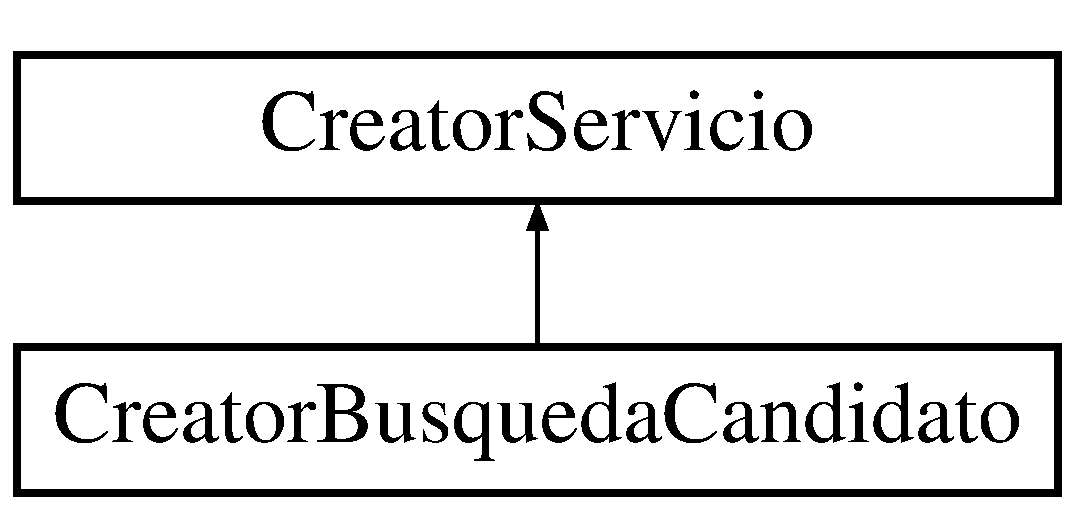
\includegraphics[height=2.000000cm]{classCreatorBusquedaCandidato}
\end{center}
\end{figure}
\subsection*{Public Member Functions}
\begin{DoxyCompactItemize}
\item 
{\bfseries Creator\+Busqueda\+Candidato} (\hyperlink{classAdministradorCandidatos}{Administrador\+Candidatos} $\ast$administrador\+Candidatos, \hyperlink{classMensajeHTTPRequest}{Mensaje\+H\+T\+T\+P\+Request} $\ast$mensaje\+H\+T\+TP, \hyperlink{classSesionesDeUsuarios}{Sesiones\+De\+Usuarios} $\ast$sesiones)\hypertarget{classCreatorBusquedaCandidato_a1543ea23204ada71e210f018722ea18a}{}\label{classCreatorBusquedaCandidato_a1543ea23204ada71e210f018722ea18a}

\end{DoxyCompactItemize}
\subsection*{Additional Inherited Members}


The documentation for this class was generated from the following files\+:\begin{DoxyCompactItemize}
\item 
Appserver/src/servicios/Creator\+Busqueda\+Candidato.\+h\item 
Appserver/src/servicios/Creator\+Busqueda\+Candidato.\+cpp\end{DoxyCompactItemize}

\hypertarget{classCreatorChat}{}\section{Creator\+Chat Class Reference}
\label{classCreatorChat}\index{Creator\+Chat@{Creator\+Chat}}
Inheritance diagram for Creator\+Chat\+:\begin{figure}[H]
\begin{center}
\leavevmode
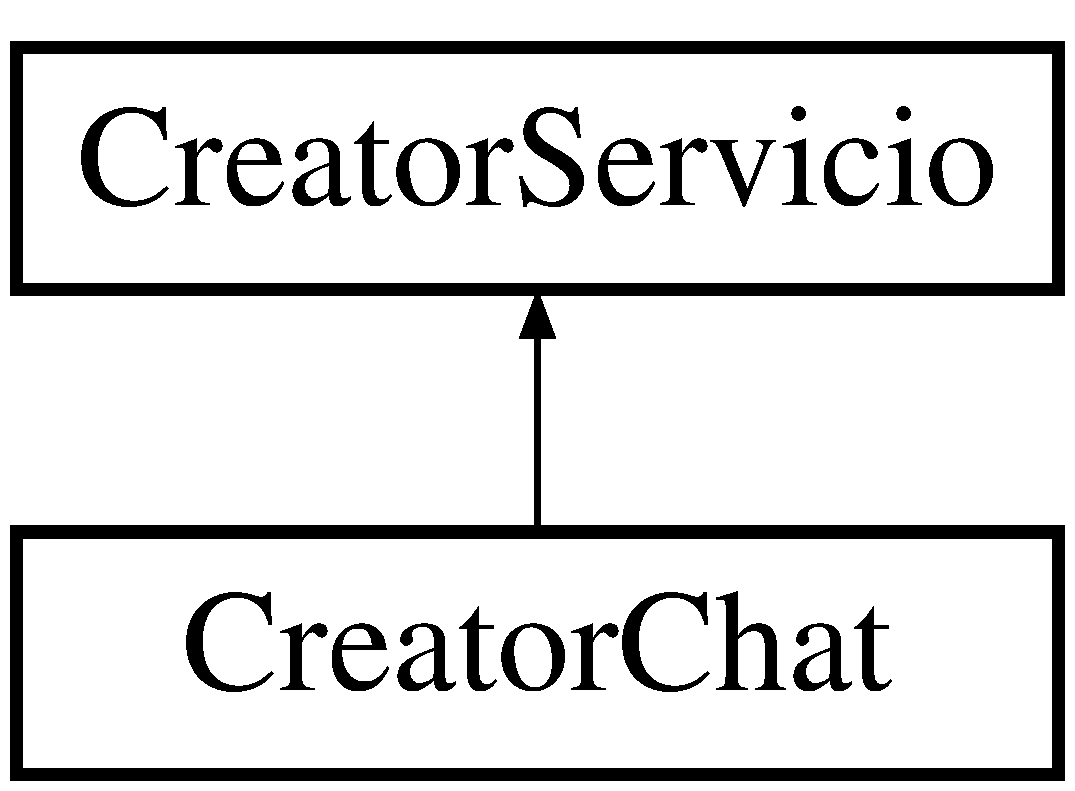
\includegraphics[height=2.000000cm]{classCreatorChat}
\end{center}
\end{figure}
\subsection*{Public Member Functions}
\begin{DoxyCompactItemize}
\item 
{\bfseries Creator\+Chat} (\hyperlink{classMensajero}{Mensajero} $\ast$mensajero, \hyperlink{classMensajeHTTPRequest}{Mensaje\+H\+T\+T\+P\+Request} $\ast$mensaje\+H\+T\+TP, \hyperlink{classSesionesDeUsuarios}{Sesiones\+De\+Usuarios} $\ast$sesiones, \hyperlink{classConversaciones}{Conversaciones} $\ast$conversaciones)\hypertarget{classCreatorChat_a07a803e2f80c4a9e4103ae8e2b56daaa}{}\label{classCreatorChat_a07a803e2f80c4a9e4103ae8e2b56daaa}

\end{DoxyCompactItemize}
\subsection*{Additional Inherited Members}


The documentation for this class was generated from the following files\+:\begin{DoxyCompactItemize}
\item 
Appserver/src/servicios/Creator\+Chat.\+h\item 
Appserver/src/servicios/Creator\+Chat.\+cpp\end{DoxyCompactItemize}

\hypertarget{classCreatorEliminacion}{}\section{Creator\+Eliminacion Class Reference}
\label{classCreatorEliminacion}\index{Creator\+Eliminacion@{Creator\+Eliminacion}}
Inheritance diagram for Creator\+Eliminacion\+:\begin{figure}[H]
\begin{center}
\leavevmode
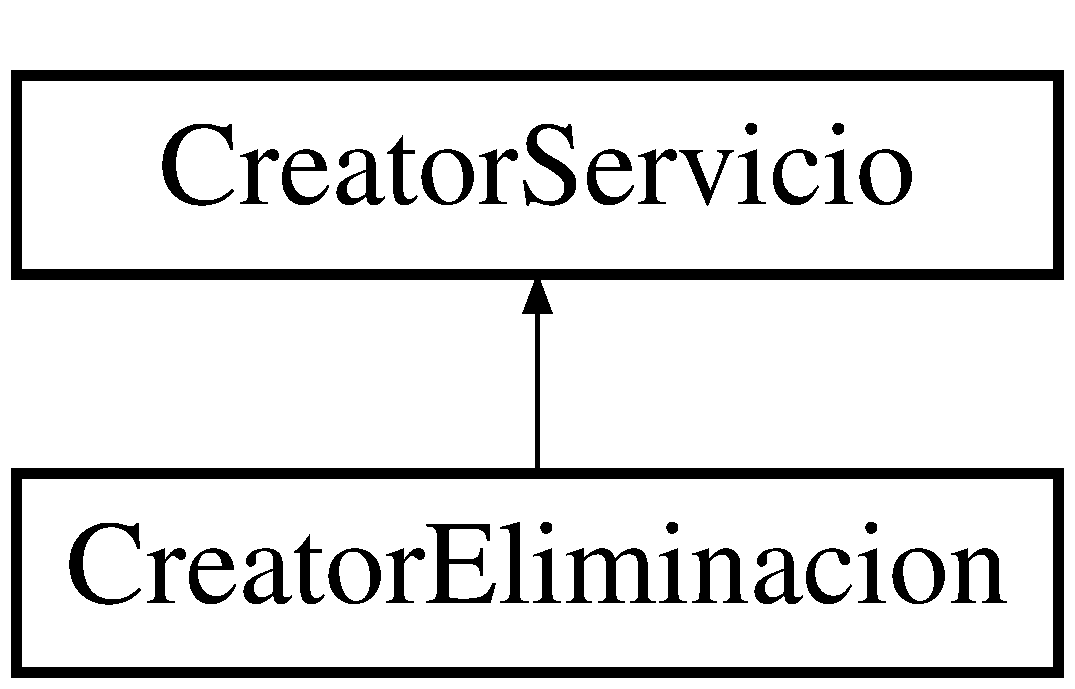
\includegraphics[height=2.000000cm]{classCreatorEliminacion}
\end{center}
\end{figure}
\subsection*{Public Member Functions}
\begin{DoxyCompactItemize}
\item 
{\bfseries Creator\+Eliminacion} (\hyperlink{classSharedDataBase}{Shared\+Data\+Base} $\ast$shared, \hyperlink{classMensajeHTTPRequest}{Mensaje\+H\+T\+T\+P\+Request} $\ast$mensaje\+H\+T\+TP, \hyperlink{classCredencialesDeUsuarios}{Credenciales\+De\+Usuarios} $\ast$credenciales, \hyperlink{classSesionesDeUsuarios}{Sesiones\+De\+Usuarios} $\ast$sesiones)\hypertarget{classCreatorEliminacion_a9df93cdf1d8c07c9a26fd0647fffdfa6}{}\label{classCreatorEliminacion_a9df93cdf1d8c07c9a26fd0647fffdfa6}

\end{DoxyCompactItemize}
\subsection*{Additional Inherited Members}


The documentation for this class was generated from the following files\+:\begin{DoxyCompactItemize}
\item 
Appserver/src/servicios/Creator\+Eliminacion.\+h\item 
Appserver/src/servicios/Creator\+Eliminacion.\+cpp\end{DoxyCompactItemize}

\hypertarget{classCreatorLogin}{}\section{Creator\+Login Class Reference}
\label{classCreatorLogin}\index{Creator\+Login@{Creator\+Login}}
Inheritance diagram for Creator\+Login\+:\begin{figure}[H]
\begin{center}
\leavevmode
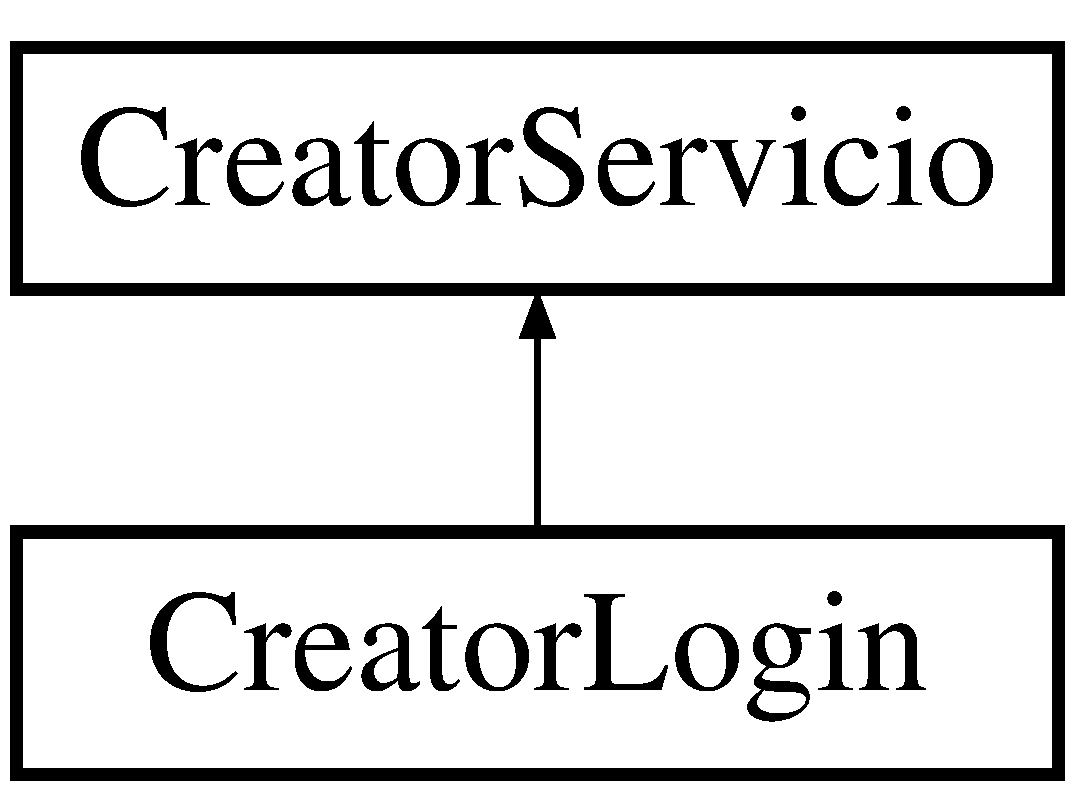
\includegraphics[height=2.000000cm]{classCreatorLogin}
\end{center}
\end{figure}
\subsection*{Public Member Functions}
\begin{DoxyCompactItemize}
\item 
{\bfseries Creator\+Login} (\hyperlink{classSesionesDeUsuarios}{Sesiones\+De\+Usuarios} $\ast$sesiones\+De\+Usuarios, \hyperlink{classMensajeHTTPRequest}{Mensaje\+H\+T\+T\+P\+Request} mensaje\+H\+T\+TP, \hyperlink{classCredencialesDeUsuarios}{Credenciales\+De\+Usuarios} $\ast$credenciales)\hypertarget{classCreatorLogin_aacbb6757418fff2e4ac679faef158120}{}\label{classCreatorLogin_aacbb6757418fff2e4ac679faef158120}

\end{DoxyCompactItemize}
\subsection*{Additional Inherited Members}


The documentation for this class was generated from the following files\+:\begin{DoxyCompactItemize}
\item 
Appserver/src/servicios/Creator\+Login.\+h\item 
Appserver/src/servicios/Creator\+Login.\+cpp\end{DoxyCompactItemize}

\hypertarget{classCreatorModificarFoto}{}\section{Creator\+Modificar\+Foto Class Reference}
\label{classCreatorModificarFoto}\index{Creator\+Modificar\+Foto@{Creator\+Modificar\+Foto}}
Inheritance diagram for Creator\+Modificar\+Foto\+:\begin{figure}[H]
\begin{center}
\leavevmode
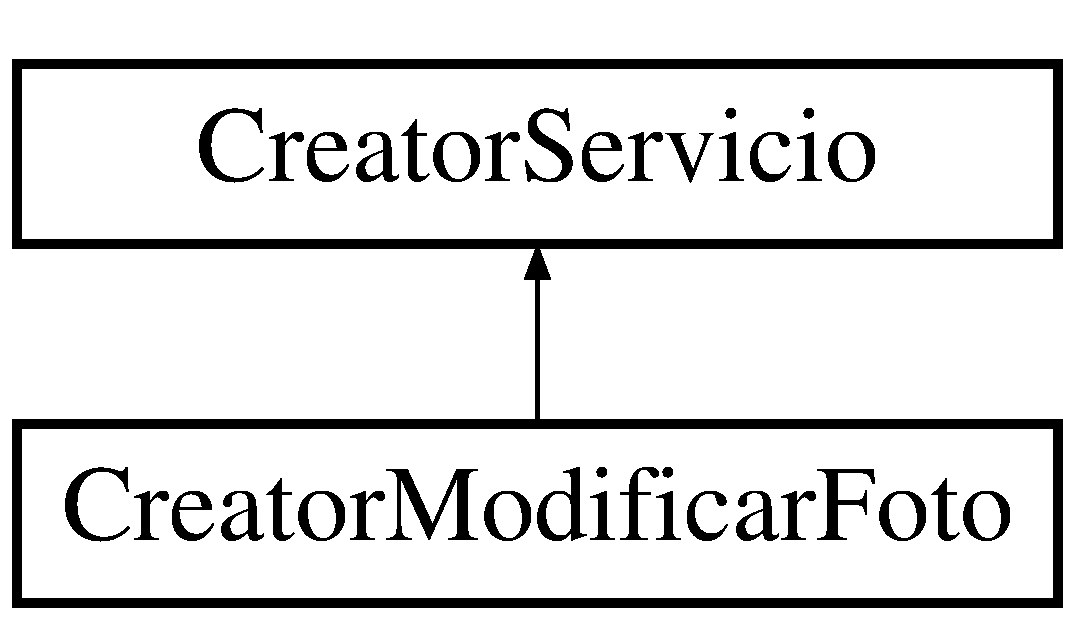
\includegraphics[height=2.000000cm]{classCreatorModificarFoto}
\end{center}
\end{figure}
\subsection*{Public Member Functions}
\begin{DoxyCompactItemize}
\item 
{\bfseries Creator\+Modificar\+Foto} (\hyperlink{classSharedDataBase}{Shared\+Data\+Base} $\ast$shared, \hyperlink{classMensajeHTTPRequest}{Mensaje\+H\+T\+T\+P\+Request} $\ast$mensaje\+H\+T\+TP, \hyperlink{classSesionesDeUsuarios}{Sesiones\+De\+Usuarios} $\ast$sesiones, \hyperlink{classCredencialesDeUsuarios}{Credenciales\+De\+Usuarios} $\ast$credenciales)\hypertarget{classCreatorModificarFoto_ad6030abac72b7f2facb579a764d5abab}{}\label{classCreatorModificarFoto_ad6030abac72b7f2facb579a764d5abab}

\end{DoxyCompactItemize}
\subsection*{Additional Inherited Members}


The documentation for this class was generated from the following files\+:\begin{DoxyCompactItemize}
\item 
Appserver/src/servicios/Creator\+Modificar\+Foto.\+h\item 
Appserver/src/servicios/Creator\+Modificar\+Foto.\+cpp\end{DoxyCompactItemize}

\hypertarget{classCreatorRegistro}{}\section{Creator\+Registro Class Reference}
\label{classCreatorRegistro}\index{Creator\+Registro@{Creator\+Registro}}
Inheritance diagram for Creator\+Registro\+:\begin{figure}[H]
\begin{center}
\leavevmode
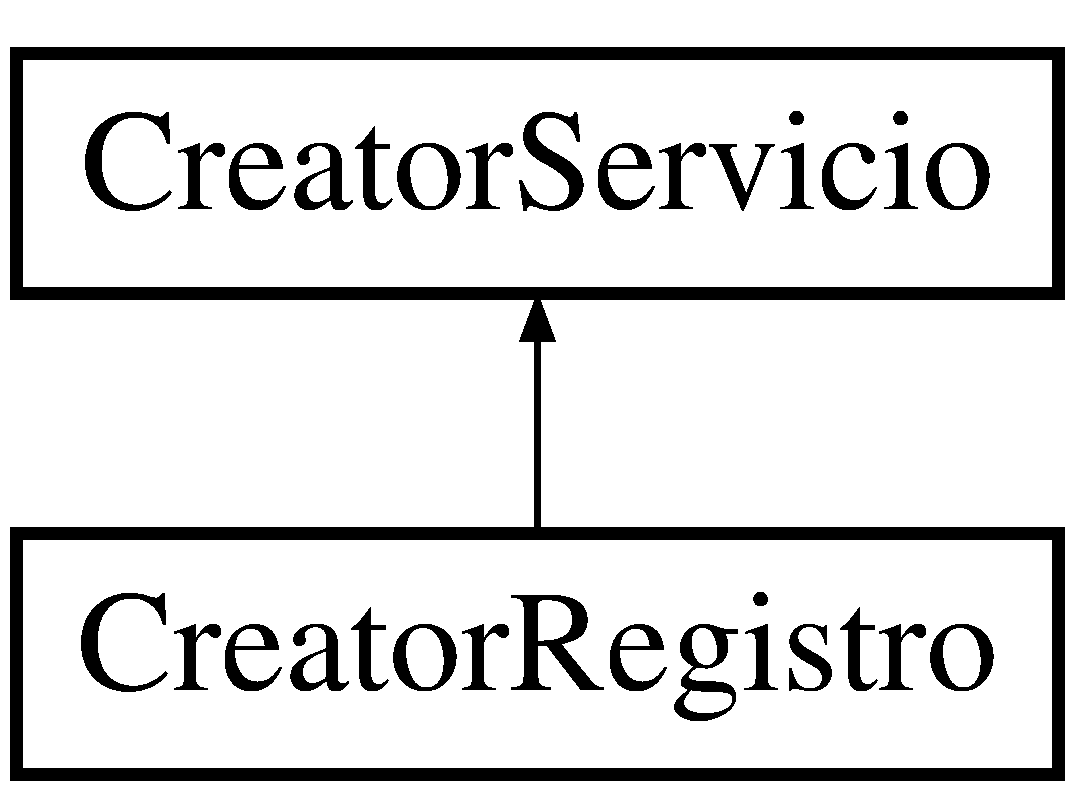
\includegraphics[height=2.000000cm]{classCreatorRegistro}
\end{center}
\end{figure}
\subsection*{Public Member Functions}
\begin{DoxyCompactItemize}
\item 
{\bfseries Creator\+Registro} (\hyperlink{classSharedDataBase}{Shared\+Data\+Base} $\ast$shared, \hyperlink{classMensajeHTTPRequest}{Mensaje\+H\+T\+T\+P\+Request} mensaje\+H\+T\+TP, \hyperlink{classCredencialesDeUsuarios}{Credenciales\+De\+Usuarios} $\ast$credenciales, \hyperlink{classAdministradorCandidatos}{Administrador\+Candidatos} $\ast$administrador\+Candidatos)\hypertarget{classCreatorRegistro_a7c2d0dbdd63f69884c557f3d368e5484}{}\label{classCreatorRegistro_a7c2d0dbdd63f69884c557f3d368e5484}

\end{DoxyCompactItemize}
\subsection*{Additional Inherited Members}


The documentation for this class was generated from the following files\+:\begin{DoxyCompactItemize}
\item 
Appserver/src/servicios/Creator\+Registro.\+h\item 
Appserver/src/servicios/Creator\+Registro.\+cpp\end{DoxyCompactItemize}

\hypertarget{classCreatorServicio}{}\section{Creator\+Servicio Class Reference}
\label{classCreatorServicio}\index{Creator\+Servicio@{Creator\+Servicio}}
Inheritance diagram for Creator\+Servicio\+:\begin{figure}[H]
\begin{center}
\leavevmode
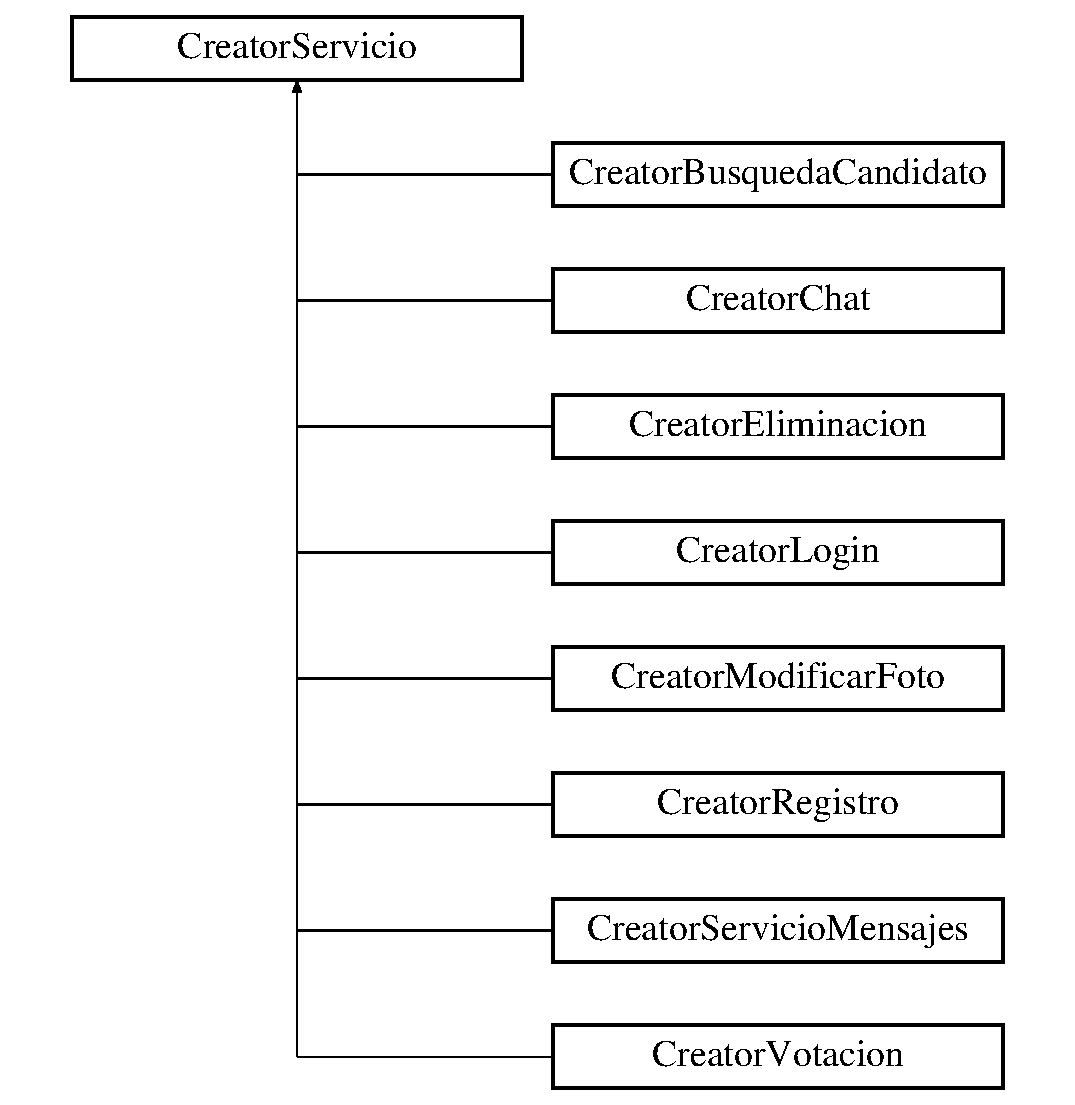
\includegraphics[height=9.000000cm]{classCreatorServicio}
\end{center}
\end{figure}
\subsection*{Public Member Functions}
\begin{DoxyCompactItemize}
\item 
\hyperlink{classServicio}{Servicio} $\ast$ {\bfseries get\+Servicio} ()\hypertarget{classCreatorServicio_a042626a63aeae5c93e5bba72bcf8300c}{}\label{classCreatorServicio_a042626a63aeae5c93e5bba72bcf8300c}

\end{DoxyCompactItemize}
\subsection*{Protected Attributes}
\begin{DoxyCompactItemize}
\item 
\hyperlink{classServicio}{Servicio} $\ast$ {\bfseries servicio}\hypertarget{classCreatorServicio_a1b40845a249b255264aabf6e347cdb05}{}\label{classCreatorServicio_a1b40845a249b255264aabf6e347cdb05}

\end{DoxyCompactItemize}


The documentation for this class was generated from the following files\+:\begin{DoxyCompactItemize}
\item 
Appserver/src/servicios/Creator\+Servicio.\+h\item 
Appserver/src/servicios/Creator\+Servicio.\+cpp\end{DoxyCompactItemize}

\hypertarget{classCreatorServicioMensajes}{}\section{Creator\+Servicio\+Mensajes Class Reference}
\label{classCreatorServicioMensajes}\index{Creator\+Servicio\+Mensajes@{Creator\+Servicio\+Mensajes}}
Inheritance diagram for Creator\+Servicio\+Mensajes\+:\begin{figure}[H]
\begin{center}
\leavevmode
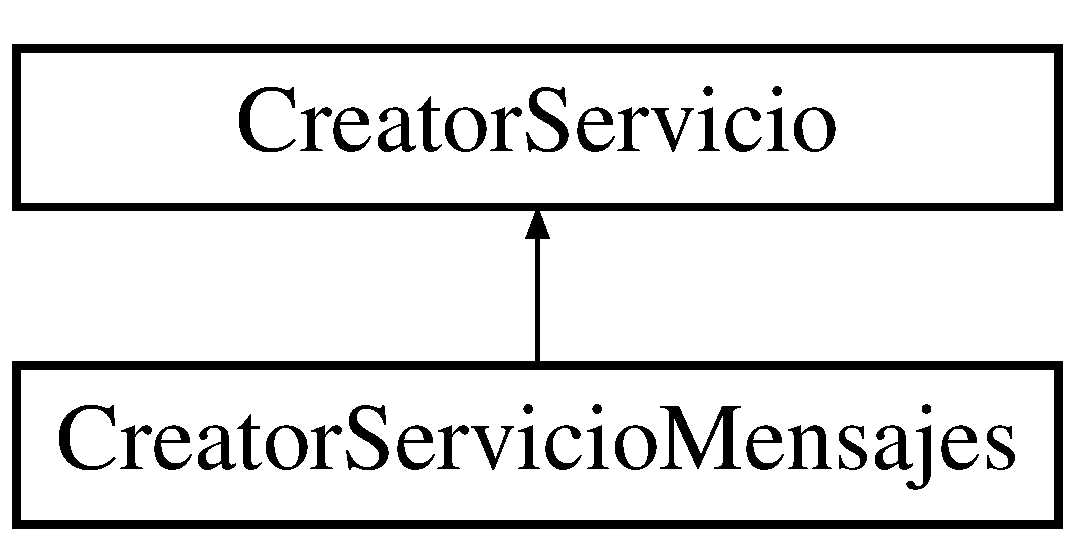
\includegraphics[height=2.000000cm]{classCreatorServicioMensajes}
\end{center}
\end{figure}
\subsection*{Public Member Functions}
\begin{DoxyCompactItemize}
\item 
{\bfseries Creator\+Servicio\+Mensajes} (\hyperlink{classMensajeHTTPRequest}{Mensaje\+H\+T\+T\+P\+Request} $\ast$mensaje\+H\+T\+TP, \hyperlink{classSesionesDeUsuarios}{Sesiones\+De\+Usuarios} $\ast$sesiones, \hyperlink{classConversaciones}{Conversaciones} $\ast$conversaciones)\hypertarget{classCreatorServicioMensajes_aa580f0c16e6ecf818f8a9a2a28ef2ed0}{}\label{classCreatorServicioMensajes_aa580f0c16e6ecf818f8a9a2a28ef2ed0}

\end{DoxyCompactItemize}
\subsection*{Additional Inherited Members}


The documentation for this class was generated from the following files\+:\begin{DoxyCompactItemize}
\item 
Appserver/src/servicios/Creator\+Servicio\+Mensajes.\+h\item 
Appserver/src/servicios/Creator\+Servicio\+Mensajes.\+cpp\end{DoxyCompactItemize}

\hypertarget{classCreatorVotacion}{}\section{Creator\+Votacion Class Reference}
\label{classCreatorVotacion}\index{Creator\+Votacion@{Creator\+Votacion}}
Inheritance diagram for Creator\+Votacion\+:\begin{figure}[H]
\begin{center}
\leavevmode
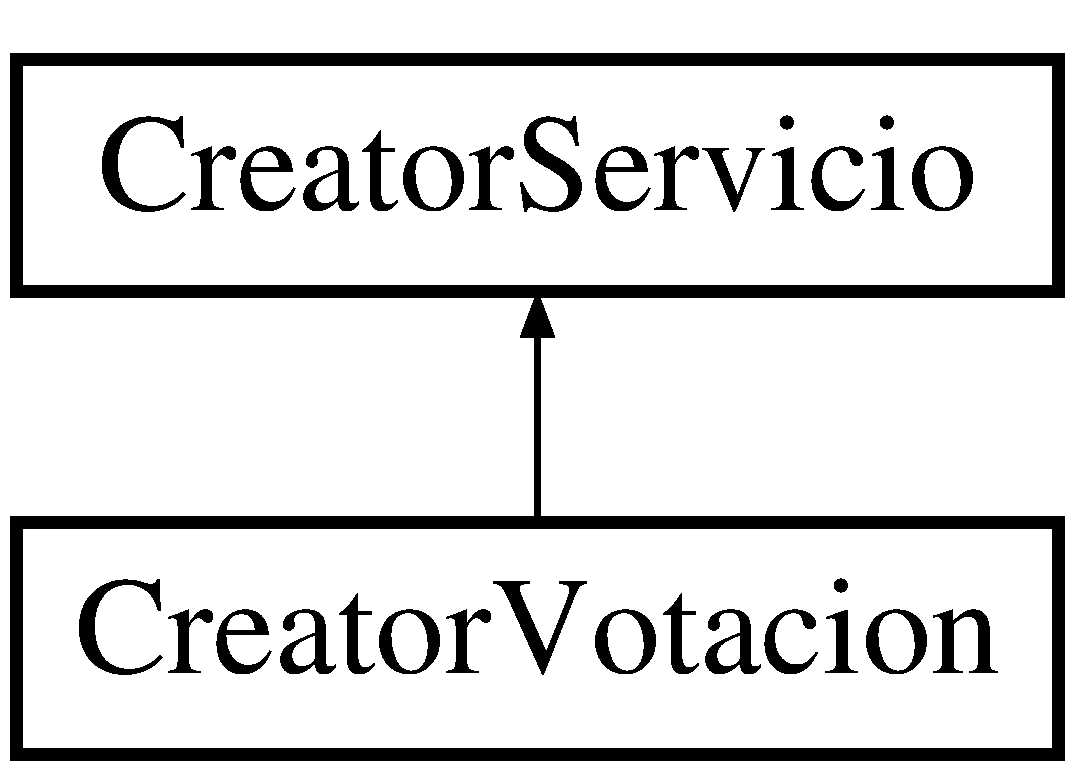
\includegraphics[height=2.000000cm]{classCreatorVotacion}
\end{center}
\end{figure}
\subsection*{Public Member Functions}
\begin{DoxyCompactItemize}
\item 
{\bfseries Creator\+Votacion} (\hyperlink{classSharedDataBase}{Shared\+Data\+Base} $\ast$shared, \hyperlink{classMensajero}{Mensajero} $\ast$mensajero, \hyperlink{classMensajeHTTPRequest}{Mensaje\+H\+T\+T\+P\+Request} $\ast$mensaje\+H\+T\+TP, \hyperlink{classSesionesDeUsuarios}{Sesiones\+De\+Usuarios} $\ast$sesiones, \hyperlink{classAdministradorCandidatos}{Administrador\+Candidatos} $\ast$administrador\+Candidatos)\hypertarget{classCreatorVotacion_a451c2e776b90aca07dc6c0aecb75ee0a}{}\label{classCreatorVotacion_a451c2e776b90aca07dc6c0aecb75ee0a}

\end{DoxyCompactItemize}
\subsection*{Additional Inherited Members}


The documentation for this class was generated from the following files\+:\begin{DoxyCompactItemize}
\item 
Appserver/src/servicios/Creator\+Votacion.\+h\item 
Appserver/src/servicios/Creator\+Votacion.\+cpp\end{DoxyCompactItemize}

\hypertarget{classCredencialesDeUsuarios}{}\section{Credenciales\+De\+Usuarios Class Reference}
\label{classCredencialesDeUsuarios}\index{Credenciales\+De\+Usuarios@{Credenciales\+De\+Usuarios}}
\subsection*{Public Member Functions}
\begin{DoxyCompactItemize}
\item 
{\bfseries Credenciales\+De\+Usuarios} (string ruta)\hypertarget{classCredencialesDeUsuarios_a15b7a889687dc843bd14f898d77ce08c}{}\label{classCredencialesDeUsuarios_a15b7a889687dc843bd14f898d77ce08c}

\item 
bool {\bfseries validar\+Credenciales} (string usuario, string password)\hypertarget{classCredencialesDeUsuarios_aaebcd26aecf776d7ed0db42a6afb7a5f}{}\label{classCredencialesDeUsuarios_aaebcd26aecf776d7ed0db42a6afb7a5f}

\item 
bool {\bfseries agregar\+Nuevo\+Usuario} (string usuario, string password, int id\+Usuario)\hypertarget{classCredencialesDeUsuarios_ab4602ff8edf46aecf52aa7063874eb6a}{}\label{classCredencialesDeUsuarios_ab4602ff8edf46aecf52aa7063874eb6a}

\item 
bool {\bfseries existe\+Usuario} (string usuario)\hypertarget{classCredencialesDeUsuarios_a0ceb2bbaf06917e3f9335f212cf8dc82}{}\label{classCredencialesDeUsuarios_a0ceb2bbaf06917e3f9335f212cf8dc82}

\item 
int {\bfseries get\+I\+D\+Shared\+De} (string usuario)\hypertarget{classCredencialesDeUsuarios_aa495a2cc2e0d3bb9015c9ef2443372d8}{}\label{classCredencialesDeUsuarios_aa495a2cc2e0d3bb9015c9ef2443372d8}

\item 
void {\bfseries eliminiar\+Usuario} (string usuario)\hypertarget{classCredencialesDeUsuarios_aa033613566beb441972f09f502178f4f}{}\label{classCredencialesDeUsuarios_aa033613566beb441972f09f502178f4f}

\end{DoxyCompactItemize}


The documentation for this class was generated from the following files\+:\begin{DoxyCompactItemize}
\item 
Appserver/src/servicios/Credenciales\+De\+Usuarios.\+h\item 
Appserver/src/servicios/Credenciales\+De\+Usuarios.\+cpp\end{DoxyCompactItemize}

\hypertarget{structcs__base64__ctx}{}\section{cs\+\_\+base64\+\_\+ctx Struct Reference}
\label{structcs__base64__ctx}\index{cs\+\_\+base64\+\_\+ctx@{cs\+\_\+base64\+\_\+ctx}}
\subsection*{Public Attributes}
\begin{DoxyCompactItemize}
\item 
cs\+\_\+base64\+\_\+putc\+\_\+t {\bfseries b64\+\_\+putc}\hypertarget{structcs__base64__ctx_a59b8384fbdd1681555a9dd18ed6585ae}{}\label{structcs__base64__ctx_a59b8384fbdd1681555a9dd18ed6585ae}

\item 
unsigned char {\bfseries chunk} \mbox{[}3\mbox{]}\hypertarget{structcs__base64__ctx_a209b5eff716d6a1850cca128ed5b070e}{}\label{structcs__base64__ctx_a209b5eff716d6a1850cca128ed5b070e}

\item 
int {\bfseries chunk\+\_\+size}\hypertarget{structcs__base64__ctx_a5753baf57fe83161369e2270d57e4a9e}{}\label{structcs__base64__ctx_a5753baf57fe83161369e2270d57e4a9e}

\item 
void $\ast$ {\bfseries user\+\_\+data}\hypertarget{structcs__base64__ctx_ac6023cc2887001835a99b6a71db9f43b}{}\label{structcs__base64__ctx_ac6023cc2887001835a99b6a71db9f43b}

\end{DoxyCompactItemize}


The documentation for this struct was generated from the following file\+:\begin{DoxyCompactItemize}
\item 
Appserver/src/external/mongoose/mongoose.\+h\end{DoxyCompactItemize}

\hypertarget{structcs__sha1__ctx}{}\section{cs\+\_\+sha1\+\_\+ctx Struct Reference}
\label{structcs__sha1__ctx}\index{cs\+\_\+sha1\+\_\+ctx@{cs\+\_\+sha1\+\_\+ctx}}
\subsection*{Public Attributes}
\begin{DoxyCompactItemize}
\item 
uint32\+\_\+t {\bfseries state} \mbox{[}5\mbox{]}\hypertarget{structcs__sha1__ctx_aaec67b16b157c16a771df82ec41220b0}{}\label{structcs__sha1__ctx_aaec67b16b157c16a771df82ec41220b0}

\item 
uint32\+\_\+t {\bfseries count} \mbox{[}2\mbox{]}\hypertarget{structcs__sha1__ctx_af6258c6cb812c334f1a287e2d6b9ea09}{}\label{structcs__sha1__ctx_af6258c6cb812c334f1a287e2d6b9ea09}

\item 
unsigned char {\bfseries buffer} \mbox{[}64\mbox{]}\hypertarget{structcs__sha1__ctx_ac7c9295501f0e13de5b0db4305a2719b}{}\label{structcs__sha1__ctx_ac7c9295501f0e13de5b0db4305a2719b}

\end{DoxyCompactItemize}


The documentation for this struct was generated from the following file\+:\begin{DoxyCompactItemize}
\item 
Appserver/src/external/mongoose/mongoose.\+h\end{DoxyCompactItemize}

\hypertarget{structctl__msg}{}\section{ctl\+\_\+msg Struct Reference}
\label{structctl__msg}\index{ctl\+\_\+msg@{ctl\+\_\+msg}}
\subsection*{Public Attributes}
\begin{DoxyCompactItemize}
\item 
mg\+\_\+event\+\_\+handler\+\_\+t {\bfseries callback}\hypertarget{structctl__msg_a62d9f57eca85bcecf123ae9046d97972}{}\label{structctl__msg_a62d9f57eca85bcecf123ae9046d97972}

\item 
char {\bfseries message} \mbox{[}M\+G\+\_\+\+C\+T\+L\+\_\+\+M\+S\+G\+\_\+\+M\+E\+S\+S\+A\+G\+E\+\_\+\+S\+I\+ZE\mbox{]}\hypertarget{structctl__msg_a07e117d1bf333976cd03507b0c1538b0}{}\label{structctl__msg_a07e117d1bf333976cd03507b0c1538b0}

\end{DoxyCompactItemize}


The documentation for this struct was generated from the following file\+:\begin{DoxyCompactItemize}
\item 
Appserver/src/external/mongoose/mongoose.\+c\end{DoxyCompactItemize}

\hypertarget{structrocksdb_1_1CuckooTableOptions}{}\section{rocksdb\+:\+:Cuckoo\+Table\+Options Struct Reference}
\label{structrocksdb_1_1CuckooTableOptions}\index{rocksdb\+::\+Cuckoo\+Table\+Options@{rocksdb\+::\+Cuckoo\+Table\+Options}}
\subsection*{Public Attributes}
\begin{DoxyCompactItemize}
\item 
double {\bfseries hash\+\_\+table\+\_\+ratio} = 0.\+9\hypertarget{structrocksdb_1_1CuckooTableOptions_a63a45d534a355a9f630032188e3abe52}{}\label{structrocksdb_1_1CuckooTableOptions_a63a45d534a355a9f630032188e3abe52}

\item 
uint32\+\_\+t {\bfseries max\+\_\+search\+\_\+depth} = 100\hypertarget{structrocksdb_1_1CuckooTableOptions_a679f19302046a5036e00a6b0327fde64}{}\label{structrocksdb_1_1CuckooTableOptions_a679f19302046a5036e00a6b0327fde64}

\item 
uint32\+\_\+t {\bfseries cuckoo\+\_\+block\+\_\+size} = 5\hypertarget{structrocksdb_1_1CuckooTableOptions_a1652482a3f24a4996d3f0e3c58c0c420}{}\label{structrocksdb_1_1CuckooTableOptions_a1652482a3f24a4996d3f0e3c58c0c420}

\item 
bool {\bfseries identity\+\_\+as\+\_\+first\+\_\+hash} = false\hypertarget{structrocksdb_1_1CuckooTableOptions_a4f2e21b88e5c6386088bd5a84a4335dc}{}\label{structrocksdb_1_1CuckooTableOptions_a4f2e21b88e5c6386088bd5a84a4335dc}

\item 
bool {\bfseries use\+\_\+module\+\_\+hash} = true\hypertarget{structrocksdb_1_1CuckooTableOptions_a8122b5e1c72fc71b8675957609674cbc}{}\label{structrocksdb_1_1CuckooTableOptions_a8122b5e1c72fc71b8675957609674cbc}

\end{DoxyCompactItemize}


The documentation for this struct was generated from the following file\+:\begin{DoxyCompactItemize}
\item 
Appserver/src/external/rocksdb/table.\+h\end{DoxyCompactItemize}

\hypertarget{structrocksdb_1_1CuckooTablePropertyNames}{}\section{rocksdb\+:\+:Cuckoo\+Table\+Property\+Names Struct Reference}
\label{structrocksdb_1_1CuckooTablePropertyNames}\index{rocksdb\+::\+Cuckoo\+Table\+Property\+Names@{rocksdb\+::\+Cuckoo\+Table\+Property\+Names}}
\subsection*{Static Public Attributes}
\begin{DoxyCompactItemize}
\item 
static const std\+::string {\bfseries k\+Empty\+Key}\hypertarget{structrocksdb_1_1CuckooTablePropertyNames_ad2cd11615e713336c1ba656f71f2556e}{}\label{structrocksdb_1_1CuckooTablePropertyNames_ad2cd11615e713336c1ba656f71f2556e}

\item 
static const std\+::string {\bfseries k\+Value\+Length}\hypertarget{structrocksdb_1_1CuckooTablePropertyNames_a93f7e4b524dc04816b44c3f4944e64c8}{}\label{structrocksdb_1_1CuckooTablePropertyNames_a93f7e4b524dc04816b44c3f4944e64c8}

\item 
static const std\+::string {\bfseries k\+Num\+Hash\+Func}\hypertarget{structrocksdb_1_1CuckooTablePropertyNames_aa69b4578d7983c3ab2552a7f9d2799ec}{}\label{structrocksdb_1_1CuckooTablePropertyNames_aa69b4578d7983c3ab2552a7f9d2799ec}

\item 
static const std\+::string {\bfseries k\+Cuckoo\+Block\+Size}\hypertarget{structrocksdb_1_1CuckooTablePropertyNames_ace537633de4c4d5bf9da30b275b3389e}{}\label{structrocksdb_1_1CuckooTablePropertyNames_ace537633de4c4d5bf9da30b275b3389e}

\item 
static const std\+::string {\bfseries k\+Hash\+Table\+Size}\hypertarget{structrocksdb_1_1CuckooTablePropertyNames_ae0707146bab108f6dd308342da9e5f6d}{}\label{structrocksdb_1_1CuckooTablePropertyNames_ae0707146bab108f6dd308342da9e5f6d}

\item 
static const std\+::string {\bfseries k\+Is\+Last\+Level}\hypertarget{structrocksdb_1_1CuckooTablePropertyNames_ad03ecf81daaeef52a6a3e09b62f8f59e}{}\label{structrocksdb_1_1CuckooTablePropertyNames_ad03ecf81daaeef52a6a3e09b62f8f59e}

\item 
static const std\+::string {\bfseries k\+Identity\+As\+First\+Hash}\hypertarget{structrocksdb_1_1CuckooTablePropertyNames_a0b59bf0c59b245cd1f31d83d27c11c65}{}\label{structrocksdb_1_1CuckooTablePropertyNames_a0b59bf0c59b245cd1f31d83d27c11c65}

\item 
static const std\+::string {\bfseries k\+Use\+Module\+Hash}\hypertarget{structrocksdb_1_1CuckooTablePropertyNames_aa00cabaf9a7cee4339b715b1a495fafb}{}\label{structrocksdb_1_1CuckooTablePropertyNames_aa00cabaf9a7cee4339b715b1a495fafb}

\item 
static const std\+::string {\bfseries k\+User\+Key\+Length}\hypertarget{structrocksdb_1_1CuckooTablePropertyNames_a9da1124e92125902c58cd7f78be7d488}{}\label{structrocksdb_1_1CuckooTablePropertyNames_a9da1124e92125902c58cd7f78be7d488}

\end{DoxyCompactItemize}


The documentation for this struct was generated from the following file\+:\begin{DoxyCompactItemize}
\item 
Appserver/src/external/rocksdb/table.\+h\end{DoxyCompactItemize}

\hypertarget{classrocksdb_1_1Cursor}{}\section{rocksdb\+:\+:Cursor Class Reference}
\label{classrocksdb_1_1Cursor}\index{rocksdb\+::\+Cursor@{rocksdb\+::\+Cursor}}
\subsection*{Public Member Functions}
\begin{DoxyCompactItemize}
\item 
virtual bool {\bfseries Valid} () const =0\hypertarget{classrocksdb_1_1Cursor_ab0f9db8bcb8dde0cd98c8af7f0b90d62}{}\label{classrocksdb_1_1Cursor_ab0f9db8bcb8dde0cd98c8af7f0b90d62}

\item 
virtual void {\bfseries Next} ()=0\hypertarget{classrocksdb_1_1Cursor_ad70946cd8e18b40bcbda6e85fe8c24e0}{}\label{classrocksdb_1_1Cursor_ad70946cd8e18b40bcbda6e85fe8c24e0}

\item 
virtual const \hyperlink{classrocksdb_1_1JSONDocument}{J\+S\+O\+N\+Document} \& {\bfseries document} () const =0\hypertarget{classrocksdb_1_1Cursor_ac823ca7c2c4e3db19c67c9636ad31be1}{}\label{classrocksdb_1_1Cursor_ac823ca7c2c4e3db19c67c9636ad31be1}

\item 
virtual \hyperlink{classrocksdb_1_1Status}{Status} {\bfseries status} () const =0\hypertarget{classrocksdb_1_1Cursor_a2e7e4a0c21f9a9702a19c1af4090a6c7}{}\label{classrocksdb_1_1Cursor_a2e7e4a0c21f9a9702a19c1af4090a6c7}

\end{DoxyCompactItemize}


The documentation for this class was generated from the following file\+:\begin{DoxyCompactItemize}
\item 
Appserver/src/external/rocksdb/utilities/document\+\_\+db.\+h\end{DoxyCompactItemize}

\hypertarget{classrocksdb_1_1spatial_1_1Cursor}{}\section{rocksdb\+:\+:spatial\+:\+:Cursor Class Reference}
\label{classrocksdb_1_1spatial_1_1Cursor}\index{rocksdb\+::spatial\+::\+Cursor@{rocksdb\+::spatial\+::\+Cursor}}
\subsection*{Public Member Functions}
\begin{DoxyCompactItemize}
\item 
virtual bool {\bfseries Valid} () const =0\hypertarget{classrocksdb_1_1spatial_1_1Cursor_a814af270f3f0537be583c387def34a85}{}\label{classrocksdb_1_1spatial_1_1Cursor_a814af270f3f0537be583c387def34a85}

\item 
virtual void {\bfseries Next} ()=0\hypertarget{classrocksdb_1_1spatial_1_1Cursor_adffc3c8e08d5f4991083b9862561b3bd}{}\label{classrocksdb_1_1spatial_1_1Cursor_adffc3c8e08d5f4991083b9862561b3bd}

\item 
virtual const \hyperlink{classrocksdb_1_1Slice}{Slice} {\bfseries blob} ()=0\hypertarget{classrocksdb_1_1spatial_1_1Cursor_a53105d40af00f666c2adf9d7364c3b71}{}\label{classrocksdb_1_1spatial_1_1Cursor_a53105d40af00f666c2adf9d7364c3b71}

\item 
virtual const \hyperlink{classrocksdb_1_1spatial_1_1FeatureSet}{Feature\+Set} \& {\bfseries feature\+\_\+set} ()=0\hypertarget{classrocksdb_1_1spatial_1_1Cursor_aeb82ba80c3d5dc4d19e8ad08455adbb2}{}\label{classrocksdb_1_1spatial_1_1Cursor_aeb82ba80c3d5dc4d19e8ad08455adbb2}

\item 
virtual \hyperlink{classrocksdb_1_1Status}{Status} {\bfseries status} () const =0\hypertarget{classrocksdb_1_1spatial_1_1Cursor_abff34fe53160404f38165cb26d6a9a4b}{}\label{classrocksdb_1_1spatial_1_1Cursor_abff34fe53160404f38165cb26d6a9a4b}

\end{DoxyCompactItemize}


The documentation for this class was generated from the following file\+:\begin{DoxyCompactItemize}
\item 
Appserver/src/external/rocksdb/utilities/spatial\+\_\+db.\+h\end{DoxyCompactItemize}

\hypertarget{structdatosDeSesion}{}\section{datos\+De\+Sesion Struct Reference}
\label{structdatosDeSesion}\index{datos\+De\+Sesion@{datos\+De\+Sesion}}
\subsection*{Public Attributes}
\begin{DoxyCompactItemize}
\item 
string {\bfseries token}\hypertarget{structdatosDeSesion_a2a9c9ea7693b8cb14914b6fade466f31}{}\label{structdatosDeSesion_a2a9c9ea7693b8cb14914b6fade466f31}

\item 
string {\bfseries token\+G\+CM}\hypertarget{structdatosDeSesion_a4962ca4a68c82f45e7094f3543c1f647}{}\label{structdatosDeSesion_a4962ca4a68c82f45e7094f3543c1f647}

\end{DoxyCompactItemize}


The documentation for this struct was generated from the following file\+:\begin{DoxyCompactItemize}
\item 
Appserver/src/servicios/Sesiones\+De\+Usuarios.\+h\end{DoxyCompactItemize}

\hypertarget{classrocksdb_1_1DB}{}\section{rocksdb\+:\+:DB Class Reference}
\label{classrocksdb_1_1DB}\index{rocksdb\+::\+DB@{rocksdb\+::\+DB}}
Inheritance diagram for rocksdb\+:\+:DB\+:\begin{figure}[H]
\begin{center}
\leavevmode
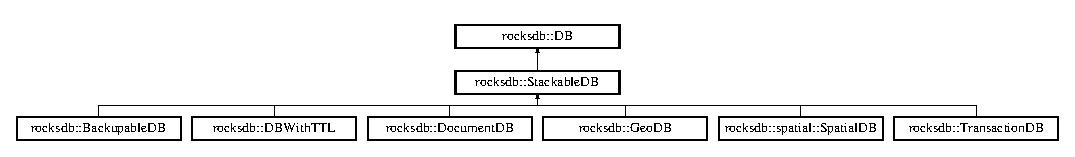
\includegraphics[height=1.666667cm]{classrocksdb_1_1DB}
\end{center}
\end{figure}
\subsection*{Classes}
\begin{DoxyCompactItemize}
\item 
struct \hyperlink{structrocksdb_1_1DB_1_1Properties}{Properties}
\end{DoxyCompactItemize}
\subsection*{Public Member Functions}
\begin{DoxyCompactItemize}
\item 
virtual \hyperlink{classrocksdb_1_1Status}{Status} {\bfseries Create\+Column\+Family} (const \hyperlink{structrocksdb_1_1ColumnFamilyOptions}{Column\+Family\+Options} \&options, const std\+::string \&column\+\_\+family\+\_\+name, \hyperlink{classrocksdb_1_1ColumnFamilyHandle}{Column\+Family\+Handle} $\ast$$\ast$handle)\hypertarget{classrocksdb_1_1DB_ab6f4cf8a955b0083fde139a70104753b}{}\label{classrocksdb_1_1DB_ab6f4cf8a955b0083fde139a70104753b}

\item 
virtual \hyperlink{classrocksdb_1_1Status}{Status} {\bfseries Drop\+Column\+Family} (\hyperlink{classrocksdb_1_1ColumnFamilyHandle}{Column\+Family\+Handle} $\ast$column\+\_\+family)\hypertarget{classrocksdb_1_1DB_af08fcb7b5334227e118e79a591b92408}{}\label{classrocksdb_1_1DB_af08fcb7b5334227e118e79a591b92408}

\item 
virtual \hyperlink{classrocksdb_1_1Status}{Status} {\bfseries Put} (const \hyperlink{structrocksdb_1_1WriteOptions}{Write\+Options} \&options, \hyperlink{classrocksdb_1_1ColumnFamilyHandle}{Column\+Family\+Handle} $\ast$column\+\_\+family, const \hyperlink{classrocksdb_1_1Slice}{Slice} \&key, const \hyperlink{classrocksdb_1_1Slice}{Slice} \&value)=0\hypertarget{classrocksdb_1_1DB_ab1731d9fde21f163083bef66454432e2}{}\label{classrocksdb_1_1DB_ab1731d9fde21f163083bef66454432e2}

\item 
virtual \hyperlink{classrocksdb_1_1Status}{Status} {\bfseries Put} (const \hyperlink{structrocksdb_1_1WriteOptions}{Write\+Options} \&options, const \hyperlink{classrocksdb_1_1Slice}{Slice} \&key, const \hyperlink{classrocksdb_1_1Slice}{Slice} \&value)\hypertarget{classrocksdb_1_1DB_a998d342c4a74b56a53e70e27c87eb2db}{}\label{classrocksdb_1_1DB_a998d342c4a74b56a53e70e27c87eb2db}

\item 
virtual \hyperlink{classrocksdb_1_1Status}{Status} {\bfseries Delete} (const \hyperlink{structrocksdb_1_1WriteOptions}{Write\+Options} \&options, \hyperlink{classrocksdb_1_1ColumnFamilyHandle}{Column\+Family\+Handle} $\ast$column\+\_\+family, const \hyperlink{classrocksdb_1_1Slice}{Slice} \&key)=0\hypertarget{classrocksdb_1_1DB_a50336757940b8c37bcf91857f11b6ad1}{}\label{classrocksdb_1_1DB_a50336757940b8c37bcf91857f11b6ad1}

\item 
virtual \hyperlink{classrocksdb_1_1Status}{Status} {\bfseries Delete} (const \hyperlink{structrocksdb_1_1WriteOptions}{Write\+Options} \&options, const \hyperlink{classrocksdb_1_1Slice}{Slice} \&key)\hypertarget{classrocksdb_1_1DB_a8fc5053ec040138744e90f0067ed6f5d}{}\label{classrocksdb_1_1DB_a8fc5053ec040138744e90f0067ed6f5d}

\item 
virtual \hyperlink{classrocksdb_1_1Status}{Status} {\bfseries Single\+Delete} (const \hyperlink{structrocksdb_1_1WriteOptions}{Write\+Options} \&options, \hyperlink{classrocksdb_1_1ColumnFamilyHandle}{Column\+Family\+Handle} $\ast$column\+\_\+family, const \hyperlink{classrocksdb_1_1Slice}{Slice} \&key)=0\hypertarget{classrocksdb_1_1DB_aacdb5c6a021a01e5ee0b9c45bef3a347}{}\label{classrocksdb_1_1DB_aacdb5c6a021a01e5ee0b9c45bef3a347}

\item 
virtual \hyperlink{classrocksdb_1_1Status}{Status} {\bfseries Single\+Delete} (const \hyperlink{structrocksdb_1_1WriteOptions}{Write\+Options} \&options, const \hyperlink{classrocksdb_1_1Slice}{Slice} \&key)\hypertarget{classrocksdb_1_1DB_a6354e7a166722545b44d751506d0239a}{}\label{classrocksdb_1_1DB_a6354e7a166722545b44d751506d0239a}

\item 
virtual \hyperlink{classrocksdb_1_1Status}{Status} {\bfseries Merge} (const \hyperlink{structrocksdb_1_1WriteOptions}{Write\+Options} \&options, \hyperlink{classrocksdb_1_1ColumnFamilyHandle}{Column\+Family\+Handle} $\ast$column\+\_\+family, const \hyperlink{classrocksdb_1_1Slice}{Slice} \&key, const \hyperlink{classrocksdb_1_1Slice}{Slice} \&value)=0\hypertarget{classrocksdb_1_1DB_ae9077bdc59ced0ea36abbe883036f4ba}{}\label{classrocksdb_1_1DB_ae9077bdc59ced0ea36abbe883036f4ba}

\item 
virtual \hyperlink{classrocksdb_1_1Status}{Status} {\bfseries Merge} (const \hyperlink{structrocksdb_1_1WriteOptions}{Write\+Options} \&options, const \hyperlink{classrocksdb_1_1Slice}{Slice} \&key, const \hyperlink{classrocksdb_1_1Slice}{Slice} \&value)\hypertarget{classrocksdb_1_1DB_a1efe3591397dba140128cf68d94c3a51}{}\label{classrocksdb_1_1DB_a1efe3591397dba140128cf68d94c3a51}

\item 
virtual \hyperlink{classrocksdb_1_1Status}{Status} {\bfseries Write} (const \hyperlink{structrocksdb_1_1WriteOptions}{Write\+Options} \&options, \hyperlink{classrocksdb_1_1WriteBatch}{Write\+Batch} $\ast$updates)=0\hypertarget{classrocksdb_1_1DB_ad5d37a09e90d0c22c9a0adca87267ebc}{}\label{classrocksdb_1_1DB_ad5d37a09e90d0c22c9a0adca87267ebc}

\item 
virtual \hyperlink{classrocksdb_1_1Status}{Status} {\bfseries Get} (const \hyperlink{structrocksdb_1_1ReadOptions}{Read\+Options} \&options, \hyperlink{classrocksdb_1_1ColumnFamilyHandle}{Column\+Family\+Handle} $\ast$column\+\_\+family, const \hyperlink{classrocksdb_1_1Slice}{Slice} \&key, std\+::string $\ast$value)=0\hypertarget{classrocksdb_1_1DB_a53885ea9306b14be2385ca8a9e664b5f}{}\label{classrocksdb_1_1DB_a53885ea9306b14be2385ca8a9e664b5f}

\item 
virtual \hyperlink{classrocksdb_1_1Status}{Status} {\bfseries Get} (const \hyperlink{structrocksdb_1_1ReadOptions}{Read\+Options} \&options, const \hyperlink{classrocksdb_1_1Slice}{Slice} \&key, std\+::string $\ast$value)\hypertarget{classrocksdb_1_1DB_ad04ed2bb886fbfb5c97af2dc3e88d8b0}{}\label{classrocksdb_1_1DB_ad04ed2bb886fbfb5c97af2dc3e88d8b0}

\item 
virtual std\+::vector$<$ \hyperlink{classrocksdb_1_1Status}{Status} $>$ {\bfseries Multi\+Get} (const \hyperlink{structrocksdb_1_1ReadOptions}{Read\+Options} \&options, const std\+::vector$<$ \hyperlink{classrocksdb_1_1ColumnFamilyHandle}{Column\+Family\+Handle} $\ast$$>$ \&column\+\_\+family, const std\+::vector$<$ \hyperlink{classrocksdb_1_1Slice}{Slice} $>$ \&keys, std\+::vector$<$ std\+::string $>$ $\ast$values)=0\hypertarget{classrocksdb_1_1DB_a5809d34b7cb788825fc65991c95a2d64}{}\label{classrocksdb_1_1DB_a5809d34b7cb788825fc65991c95a2d64}

\item 
virtual std\+::vector$<$ \hyperlink{classrocksdb_1_1Status}{Status} $>$ {\bfseries Multi\+Get} (const \hyperlink{structrocksdb_1_1ReadOptions}{Read\+Options} \&options, const std\+::vector$<$ \hyperlink{classrocksdb_1_1Slice}{Slice} $>$ \&keys, std\+::vector$<$ std\+::string $>$ $\ast$values)\hypertarget{classrocksdb_1_1DB_a608e457908d203043d7d6756ab58d5ef}{}\label{classrocksdb_1_1DB_a608e457908d203043d7d6756ab58d5ef}

\item 
virtual bool {\bfseries Key\+May\+Exist} (const \hyperlink{structrocksdb_1_1ReadOptions}{Read\+Options} \&, \hyperlink{classrocksdb_1_1ColumnFamilyHandle}{Column\+Family\+Handle} $\ast$, const \hyperlink{classrocksdb_1_1Slice}{Slice} \&, std\+::string $\ast$, bool $\ast$value\+\_\+found=nullptr)\hypertarget{classrocksdb_1_1DB_a771ca74b3c3a772e4f45169180692c06}{}\label{classrocksdb_1_1DB_a771ca74b3c3a772e4f45169180692c06}

\item 
virtual bool {\bfseries Key\+May\+Exist} (const \hyperlink{structrocksdb_1_1ReadOptions}{Read\+Options} \&options, const \hyperlink{classrocksdb_1_1Slice}{Slice} \&key, std\+::string $\ast$value, bool $\ast$value\+\_\+found=nullptr)\hypertarget{classrocksdb_1_1DB_a17165bfaf29a7b0b1fc36bf684954e53}{}\label{classrocksdb_1_1DB_a17165bfaf29a7b0b1fc36bf684954e53}

\item 
virtual \hyperlink{classrocksdb_1_1Iterator}{Iterator} $\ast$ {\bfseries New\+Iterator} (const \hyperlink{structrocksdb_1_1ReadOptions}{Read\+Options} \&options, \hyperlink{classrocksdb_1_1ColumnFamilyHandle}{Column\+Family\+Handle} $\ast$column\+\_\+family)=0\hypertarget{classrocksdb_1_1DB_ab76fb645ee6e5e1aa1e1b9f6f61c831a}{}\label{classrocksdb_1_1DB_ab76fb645ee6e5e1aa1e1b9f6f61c831a}

\item 
virtual \hyperlink{classrocksdb_1_1Iterator}{Iterator} $\ast$ {\bfseries New\+Iterator} (const \hyperlink{structrocksdb_1_1ReadOptions}{Read\+Options} \&options)\hypertarget{classrocksdb_1_1DB_a898a5baaba9ec5b0f451f2f8863ab79d}{}\label{classrocksdb_1_1DB_a898a5baaba9ec5b0f451f2f8863ab79d}

\item 
virtual \hyperlink{classrocksdb_1_1Status}{Status} {\bfseries New\+Iterators} (const \hyperlink{structrocksdb_1_1ReadOptions}{Read\+Options} \&options, const std\+::vector$<$ \hyperlink{classrocksdb_1_1ColumnFamilyHandle}{Column\+Family\+Handle} $\ast$$>$ \&column\+\_\+families, std\+::vector$<$ \hyperlink{classrocksdb_1_1Iterator}{Iterator} $\ast$$>$ $\ast$iterators)=0\hypertarget{classrocksdb_1_1DB_a1d8e4e97c149deaf44e4664f2b0efe9a}{}\label{classrocksdb_1_1DB_a1d8e4e97c149deaf44e4664f2b0efe9a}

\item 
virtual const \hyperlink{classrocksdb_1_1Snapshot}{Snapshot} $\ast$ {\bfseries Get\+Snapshot} ()=0\hypertarget{classrocksdb_1_1DB_a09ad7c62dfe7e8739732d37041d058f9}{}\label{classrocksdb_1_1DB_a09ad7c62dfe7e8739732d37041d058f9}

\item 
virtual void {\bfseries Release\+Snapshot} (const \hyperlink{classrocksdb_1_1Snapshot}{Snapshot} $\ast$snapshot)=0\hypertarget{classrocksdb_1_1DB_aedefaa4497eb584a45a818c0f05aff9b}{}\label{classrocksdb_1_1DB_aedefaa4497eb584a45a818c0f05aff9b}

\item 
virtual bool {\bfseries Get\+Property} (\hyperlink{classrocksdb_1_1ColumnFamilyHandle}{Column\+Family\+Handle} $\ast$column\+\_\+family, const \hyperlink{classrocksdb_1_1Slice}{Slice} \&property, std\+::string $\ast$value)=0\hypertarget{classrocksdb_1_1DB_a31f99bb093e4b586f3f10c04592043dc}{}\label{classrocksdb_1_1DB_a31f99bb093e4b586f3f10c04592043dc}

\item 
virtual bool {\bfseries Get\+Property} (const \hyperlink{classrocksdb_1_1Slice}{Slice} \&property, std\+::string $\ast$value)\hypertarget{classrocksdb_1_1DB_a579863b12d9adff0cb560218846c9b1f}{}\label{classrocksdb_1_1DB_a579863b12d9adff0cb560218846c9b1f}

\item 
virtual bool {\bfseries Get\+Int\+Property} (\hyperlink{classrocksdb_1_1ColumnFamilyHandle}{Column\+Family\+Handle} $\ast$column\+\_\+family, const \hyperlink{classrocksdb_1_1Slice}{Slice} \&property, uint64\+\_\+t $\ast$value)=0\hypertarget{classrocksdb_1_1DB_a76b06e26e9c0436b26034f826bfda8c0}{}\label{classrocksdb_1_1DB_a76b06e26e9c0436b26034f826bfda8c0}

\item 
virtual bool {\bfseries Get\+Int\+Property} (const \hyperlink{classrocksdb_1_1Slice}{Slice} \&property, uint64\+\_\+t $\ast$value)\hypertarget{classrocksdb_1_1DB_a0e8ae1d11f99d95db4d6e270674a9f7b}{}\label{classrocksdb_1_1DB_a0e8ae1d11f99d95db4d6e270674a9f7b}

\item 
virtual bool {\bfseries Get\+Aggregated\+Int\+Property} (const \hyperlink{classrocksdb_1_1Slice}{Slice} \&property, uint64\+\_\+t $\ast$value)=0\hypertarget{classrocksdb_1_1DB_a27ffb63934a6b2e1fdae25667f551f76}{}\label{classrocksdb_1_1DB_a27ffb63934a6b2e1fdae25667f551f76}

\item 
virtual void {\bfseries Get\+Approximate\+Sizes} (\hyperlink{classrocksdb_1_1ColumnFamilyHandle}{Column\+Family\+Handle} $\ast$column\+\_\+family, const \hyperlink{structrocksdb_1_1Range}{Range} $\ast$range, int n, uint64\+\_\+t $\ast$sizes, bool include\+\_\+memtable=false)=0\hypertarget{classrocksdb_1_1DB_a3f135e62b87497858d3abcff25b651ce}{}\label{classrocksdb_1_1DB_a3f135e62b87497858d3abcff25b651ce}

\item 
virtual void {\bfseries Get\+Approximate\+Sizes} (const \hyperlink{structrocksdb_1_1Range}{Range} $\ast$range, int n, uint64\+\_\+t $\ast$sizes, bool include\+\_\+memtable=false)\hypertarget{classrocksdb_1_1DB_a0d06bfb3ff0c90a650d1c2bb4926e6ce}{}\label{classrocksdb_1_1DB_a0d06bfb3ff0c90a650d1c2bb4926e6ce}

\item 
virtual \hyperlink{classrocksdb_1_1Status}{Status} {\bfseries Compact\+Range} (const \hyperlink{structrocksdb_1_1CompactRangeOptions}{Compact\+Range\+Options} \&options, \hyperlink{classrocksdb_1_1ColumnFamilyHandle}{Column\+Family\+Handle} $\ast$column\+\_\+family, const \hyperlink{classrocksdb_1_1Slice}{Slice} $\ast$begin, const \hyperlink{classrocksdb_1_1Slice}{Slice} $\ast$end)=0\hypertarget{classrocksdb_1_1DB_a83ca9b10138335cd4fddadd65c748882}{}\label{classrocksdb_1_1DB_a83ca9b10138335cd4fddadd65c748882}

\item 
virtual \hyperlink{classrocksdb_1_1Status}{Status} {\bfseries Compact\+Range} (const \hyperlink{structrocksdb_1_1CompactRangeOptions}{Compact\+Range\+Options} \&options, const \hyperlink{classrocksdb_1_1Slice}{Slice} $\ast$begin, const \hyperlink{classrocksdb_1_1Slice}{Slice} $\ast$end)\hypertarget{classrocksdb_1_1DB_a405ebb44a9ca8dff9fff6def599c1a94}{}\label{classrocksdb_1_1DB_a405ebb44a9ca8dff9fff6def599c1a94}

\item 
virtual \hyperlink{classrocksdb_1_1Status}{Status} {\bfseries Compact\+Range} (\hyperlink{classrocksdb_1_1ColumnFamilyHandle}{Column\+Family\+Handle} $\ast$column\+\_\+family, const \hyperlink{classrocksdb_1_1Slice}{Slice} $\ast$begin, const \hyperlink{classrocksdb_1_1Slice}{Slice} $\ast$end, bool change\+\_\+level=false, int target\+\_\+level=-\/1, uint32\+\_\+t target\+\_\+path\+\_\+id=0)\hypertarget{classrocksdb_1_1DB_a7dd130ae3133ee9390fc27436cb4ca30}{}\label{classrocksdb_1_1DB_a7dd130ae3133ee9390fc27436cb4ca30}

\item 
virtual \hyperlink{classrocksdb_1_1Status}{Status} {\bfseries Compact\+Range} (const \hyperlink{classrocksdb_1_1Slice}{Slice} $\ast$begin, const \hyperlink{classrocksdb_1_1Slice}{Slice} $\ast$end, bool change\+\_\+level=false, int target\+\_\+level=-\/1, uint32\+\_\+t target\+\_\+path\+\_\+id=0)\hypertarget{classrocksdb_1_1DB_abde04eaf7df420cd1e8b9e3a185ac7fd}{}\label{classrocksdb_1_1DB_abde04eaf7df420cd1e8b9e3a185ac7fd}

\item 
virtual \hyperlink{classrocksdb_1_1Status}{Status} {\bfseries Set\+Options} (\hyperlink{classrocksdb_1_1ColumnFamilyHandle}{Column\+Family\+Handle} $\ast$, const std\+::unordered\+\_\+map$<$ std\+::string, std\+::string $>$ \&)\hypertarget{classrocksdb_1_1DB_a28795d0bb3016cff44b19f224d7114f8}{}\label{classrocksdb_1_1DB_a28795d0bb3016cff44b19f224d7114f8}

\item 
virtual \hyperlink{classrocksdb_1_1Status}{Status} {\bfseries Set\+Options} (const std\+::unordered\+\_\+map$<$ std\+::string, std\+::string $>$ \&new\+\_\+options)\hypertarget{classrocksdb_1_1DB_aa2c805ad4ad7a1e37390d95f67502740}{}\label{classrocksdb_1_1DB_aa2c805ad4ad7a1e37390d95f67502740}

\item 
virtual \hyperlink{classrocksdb_1_1Status}{Status} {\bfseries Compact\+Files} (const \hyperlink{structrocksdb_1_1CompactionOptions}{Compaction\+Options} \&compact\+\_\+options, \hyperlink{classrocksdb_1_1ColumnFamilyHandle}{Column\+Family\+Handle} $\ast$column\+\_\+family, const std\+::vector$<$ std\+::string $>$ \&input\+\_\+file\+\_\+names, const int output\+\_\+level, const int output\+\_\+path\+\_\+id=-\/1)=0\hypertarget{classrocksdb_1_1DB_a6d291df380bb41a6737689c3d33e7d73}{}\label{classrocksdb_1_1DB_a6d291df380bb41a6737689c3d33e7d73}

\item 
virtual \hyperlink{classrocksdb_1_1Status}{Status} {\bfseries Compact\+Files} (const \hyperlink{structrocksdb_1_1CompactionOptions}{Compaction\+Options} \&compact\+\_\+options, const std\+::vector$<$ std\+::string $>$ \&input\+\_\+file\+\_\+names, const int output\+\_\+level, const int output\+\_\+path\+\_\+id=-\/1)\hypertarget{classrocksdb_1_1DB_a3158273244f418b65d9f04caff0d7368}{}\label{classrocksdb_1_1DB_a3158273244f418b65d9f04caff0d7368}

\item 
virtual \hyperlink{classrocksdb_1_1Status}{Status} {\bfseries Pause\+Background\+Work} ()=0\hypertarget{classrocksdb_1_1DB_af392b40e23a8db606e8ee220e5a58c00}{}\label{classrocksdb_1_1DB_af392b40e23a8db606e8ee220e5a58c00}

\item 
virtual \hyperlink{classrocksdb_1_1Status}{Status} {\bfseries Continue\+Background\+Work} ()=0\hypertarget{classrocksdb_1_1DB_acb9cd7be26b415f52f33e65f3c5be02e}{}\label{classrocksdb_1_1DB_acb9cd7be26b415f52f33e65f3c5be02e}

\item 
virtual \hyperlink{classrocksdb_1_1Status}{Status} {\bfseries Enable\+Auto\+Compaction} (const std\+::vector$<$ \hyperlink{classrocksdb_1_1ColumnFamilyHandle}{Column\+Family\+Handle} $\ast$$>$ \&column\+\_\+family\+\_\+handles)=0\hypertarget{classrocksdb_1_1DB_acd233aa1070ea21b4bc329fdf1fdf277}{}\label{classrocksdb_1_1DB_acd233aa1070ea21b4bc329fdf1fdf277}

\item 
virtual int {\bfseries Number\+Levels} (\hyperlink{classrocksdb_1_1ColumnFamilyHandle}{Column\+Family\+Handle} $\ast$column\+\_\+family)=0\hypertarget{classrocksdb_1_1DB_a6581ba7d28b51491faebe55a7df500b1}{}\label{classrocksdb_1_1DB_a6581ba7d28b51491faebe55a7df500b1}

\item 
virtual int {\bfseries Number\+Levels} ()\hypertarget{classrocksdb_1_1DB_aa8becbddfcbd7353aa3a21ef955a9c46}{}\label{classrocksdb_1_1DB_aa8becbddfcbd7353aa3a21ef955a9c46}

\item 
virtual int {\bfseries Max\+Mem\+Compaction\+Level} (\hyperlink{classrocksdb_1_1ColumnFamilyHandle}{Column\+Family\+Handle} $\ast$column\+\_\+family)=0\hypertarget{classrocksdb_1_1DB_a25dedb3ebc958c5dfff1eee4453fbd56}{}\label{classrocksdb_1_1DB_a25dedb3ebc958c5dfff1eee4453fbd56}

\item 
virtual int {\bfseries Max\+Mem\+Compaction\+Level} ()\hypertarget{classrocksdb_1_1DB_a5762e92e3e20880efd3a399c5a0e0ae5}{}\label{classrocksdb_1_1DB_a5762e92e3e20880efd3a399c5a0e0ae5}

\item 
virtual int {\bfseries Level0\+Stop\+Write\+Trigger} (\hyperlink{classrocksdb_1_1ColumnFamilyHandle}{Column\+Family\+Handle} $\ast$column\+\_\+family)=0\hypertarget{classrocksdb_1_1DB_a818ec586390892c14201b610ced44283}{}\label{classrocksdb_1_1DB_a818ec586390892c14201b610ced44283}

\item 
virtual int {\bfseries Level0\+Stop\+Write\+Trigger} ()\hypertarget{classrocksdb_1_1DB_aa9d8399659361a8d4d239d16f09d777c}{}\label{classrocksdb_1_1DB_aa9d8399659361a8d4d239d16f09d777c}

\item 
virtual const std\+::string \& {\bfseries Get\+Name} () const =0\hypertarget{classrocksdb_1_1DB_ad3dd1a5cbcd4161cc9b7aae7b0287406}{}\label{classrocksdb_1_1DB_ad3dd1a5cbcd4161cc9b7aae7b0287406}

\item 
virtual \hyperlink{classrocksdb_1_1Env}{Env} $\ast$ {\bfseries Get\+Env} () const =0\hypertarget{classrocksdb_1_1DB_aab78568f94216fcb321af22ee2803882}{}\label{classrocksdb_1_1DB_aab78568f94216fcb321af22ee2803882}

\item 
virtual const \hyperlink{structrocksdb_1_1Options}{Options} \& {\bfseries Get\+Options} (\hyperlink{classrocksdb_1_1ColumnFamilyHandle}{Column\+Family\+Handle} $\ast$column\+\_\+family) const =0\hypertarget{classrocksdb_1_1DB_aa8b1587fe656f511da075a5bc722fe27}{}\label{classrocksdb_1_1DB_aa8b1587fe656f511da075a5bc722fe27}

\item 
virtual const \hyperlink{structrocksdb_1_1Options}{Options} \& {\bfseries Get\+Options} () const\hypertarget{classrocksdb_1_1DB_a5ea0041b5bf31c38256152a698b6a6da}{}\label{classrocksdb_1_1DB_a5ea0041b5bf31c38256152a698b6a6da}

\item 
virtual const \hyperlink{structrocksdb_1_1DBOptions}{D\+B\+Options} \& {\bfseries Get\+D\+B\+Options} () const =0\hypertarget{classrocksdb_1_1DB_a3dc7a81072b8eaa75a785a3f7b094809}{}\label{classrocksdb_1_1DB_a3dc7a81072b8eaa75a785a3f7b094809}

\item 
virtual \hyperlink{classrocksdb_1_1Status}{Status} {\bfseries Flush} (const \hyperlink{structrocksdb_1_1FlushOptions}{Flush\+Options} \&options, \hyperlink{classrocksdb_1_1ColumnFamilyHandle}{Column\+Family\+Handle} $\ast$column\+\_\+family)=0\hypertarget{classrocksdb_1_1DB_afb62c428d9ffaf473bdd9ecc7568cfe5}{}\label{classrocksdb_1_1DB_afb62c428d9ffaf473bdd9ecc7568cfe5}

\item 
virtual \hyperlink{classrocksdb_1_1Status}{Status} {\bfseries Flush} (const \hyperlink{structrocksdb_1_1FlushOptions}{Flush\+Options} \&options)\hypertarget{classrocksdb_1_1DB_ae50d0a8ea55b682b6f4fe1e696f388ba}{}\label{classrocksdb_1_1DB_ae50d0a8ea55b682b6f4fe1e696f388ba}

\item 
virtual \hyperlink{classrocksdb_1_1Status}{Status} {\bfseries Sync\+W\+AL} ()=0\hypertarget{classrocksdb_1_1DB_afd06e3e012663cb19640a82b741b6884}{}\label{classrocksdb_1_1DB_afd06e3e012663cb19640a82b741b6884}

\item 
virtual Sequence\+Number {\bfseries Get\+Latest\+Sequence\+Number} () const =0\hypertarget{classrocksdb_1_1DB_a71590d8fbc17ba01c39d2067cd26a084}{}\label{classrocksdb_1_1DB_a71590d8fbc17ba01c39d2067cd26a084}

\item 
virtual \hyperlink{classrocksdb_1_1Status}{Status} {\bfseries Disable\+File\+Deletions} ()=0\hypertarget{classrocksdb_1_1DB_a03dd54471b0ab3aadbd88200b305d9a9}{}\label{classrocksdb_1_1DB_a03dd54471b0ab3aadbd88200b305d9a9}

\item 
virtual \hyperlink{classrocksdb_1_1Status}{Status} {\bfseries Enable\+File\+Deletions} (bool force=true)=0\hypertarget{classrocksdb_1_1DB_a8972bd881003084cfd646487fbe0ee0a}{}\label{classrocksdb_1_1DB_a8972bd881003084cfd646487fbe0ee0a}

\item 
virtual \hyperlink{classrocksdb_1_1Status}{Status} {\bfseries Get\+Live\+Files} (std\+::vector$<$ std\+::string $>$ \&, uint64\+\_\+t $\ast$manifest\+\_\+file\+\_\+size, bool flush\+\_\+memtable=true)=0\hypertarget{classrocksdb_1_1DB_a1c645c8ae376c0acd11a3271ec3a59ad}{}\label{classrocksdb_1_1DB_a1c645c8ae376c0acd11a3271ec3a59ad}

\item 
virtual \hyperlink{classrocksdb_1_1Status}{Status} {\bfseries Get\+Sorted\+Wal\+Files} (Vector\+Log\+Ptr \&files)=0\hypertarget{classrocksdb_1_1DB_a4cbc3ccd04ec78d0268b38397c2af029}{}\label{classrocksdb_1_1DB_a4cbc3ccd04ec78d0268b38397c2af029}

\item 
virtual \hyperlink{classrocksdb_1_1Status}{Status} {\bfseries Get\+Updates\+Since} (Sequence\+Number seq\+\_\+number, unique\+\_\+ptr$<$ \hyperlink{classrocksdb_1_1TransactionLogIterator}{Transaction\+Log\+Iterator} $>$ $\ast$iter, const \hyperlink{structrocksdb_1_1TransactionLogIterator_1_1ReadOptions}{Transaction\+Log\+Iterator\+::\+Read\+Options} \&read\+\_\+options=\hyperlink{structrocksdb_1_1TransactionLogIterator_1_1ReadOptions}{Transaction\+Log\+Iterator\+::\+Read\+Options}())=0\hypertarget{classrocksdb_1_1DB_aa604af3c08d15340565f4552acfde5cc}{}\label{classrocksdb_1_1DB_aa604af3c08d15340565f4552acfde5cc}

\item 
virtual \hyperlink{classrocksdb_1_1Status}{Status} {\bfseries Delete\+File} (std\+::string name)=0\hypertarget{classrocksdb_1_1DB_a04985803f9914f80a9f4bdd894771e2b}{}\label{classrocksdb_1_1DB_a04985803f9914f80a9f4bdd894771e2b}

\item 
virtual void {\bfseries Get\+Live\+Files\+Meta\+Data} (std\+::vector$<$ \hyperlink{structrocksdb_1_1LiveFileMetaData}{Live\+File\+Meta\+Data} $>$ $\ast$)\hypertarget{classrocksdb_1_1DB_ae7d0a66cc4f4e08e6df31db2aa48aebe}{}\label{classrocksdb_1_1DB_ae7d0a66cc4f4e08e6df31db2aa48aebe}

\item 
virtual void {\bfseries Get\+Column\+Family\+Meta\+Data} (\hyperlink{classrocksdb_1_1ColumnFamilyHandle}{Column\+Family\+Handle} $\ast$, \hyperlink{structrocksdb_1_1ColumnFamilyMetaData}{Column\+Family\+Meta\+Data} $\ast$)\hypertarget{classrocksdb_1_1DB_a0d0c02b96ac8ac35c49bf00f4ddd0021}{}\label{classrocksdb_1_1DB_a0d0c02b96ac8ac35c49bf00f4ddd0021}

\item 
void {\bfseries Get\+Column\+Family\+Meta\+Data} (\hyperlink{structrocksdb_1_1ColumnFamilyMetaData}{Column\+Family\+Meta\+Data} $\ast$metadata)\hypertarget{classrocksdb_1_1DB_a90f405c1bdced4252d8e9fd9925b95b4}{}\label{classrocksdb_1_1DB_a90f405c1bdced4252d8e9fd9925b95b4}

\item 
virtual \hyperlink{classrocksdb_1_1Status}{Status} {\bfseries Add\+File} (\hyperlink{classrocksdb_1_1ColumnFamilyHandle}{Column\+Family\+Handle} $\ast$column\+\_\+family, const std\+::string \&file\+\_\+path, bool move\+\_\+file=false)=0\hypertarget{classrocksdb_1_1DB_af02d75b05154cbb1c1fa9dcad88c26ef}{}\label{classrocksdb_1_1DB_af02d75b05154cbb1c1fa9dcad88c26ef}

\item 
virtual \hyperlink{classrocksdb_1_1Status}{Status} {\bfseries Add\+File} (const std\+::string \&file\+\_\+path, bool move\+\_\+file=false)\hypertarget{classrocksdb_1_1DB_afd2b59898d904dde210f9ab174af6bd2}{}\label{classrocksdb_1_1DB_afd2b59898d904dde210f9ab174af6bd2}

\item 
virtual \hyperlink{classrocksdb_1_1Status}{Status} {\bfseries Add\+File} (\hyperlink{classrocksdb_1_1ColumnFamilyHandle}{Column\+Family\+Handle} $\ast$column\+\_\+family, const \hyperlink{structrocksdb_1_1ExternalSstFileInfo}{External\+Sst\+File\+Info} $\ast$file\+\_\+info, bool move\+\_\+file=false)=0\hypertarget{classrocksdb_1_1DB_a41c3fb74e6f0ac69c4fc8f475384f4b1}{}\label{classrocksdb_1_1DB_a41c3fb74e6f0ac69c4fc8f475384f4b1}

\item 
virtual \hyperlink{classrocksdb_1_1Status}{Status} {\bfseries Add\+File} (const \hyperlink{structrocksdb_1_1ExternalSstFileInfo}{External\+Sst\+File\+Info} $\ast$file\+\_\+info, bool move\+\_\+file=false)\hypertarget{classrocksdb_1_1DB_a4cb68b0602b9b312abe680e7916e717f}{}\label{classrocksdb_1_1DB_a4cb68b0602b9b312abe680e7916e717f}

\item 
virtual \hyperlink{classrocksdb_1_1Status}{Status} {\bfseries Get\+Db\+Identity} (std\+::string \&identity) const =0\hypertarget{classrocksdb_1_1DB_ae25bfa14c79c2a314fb2c2b9b15c8878}{}\label{classrocksdb_1_1DB_ae25bfa14c79c2a314fb2c2b9b15c8878}

\item 
virtual \hyperlink{classrocksdb_1_1ColumnFamilyHandle}{Column\+Family\+Handle} $\ast$ {\bfseries Default\+Column\+Family} () const =0\hypertarget{classrocksdb_1_1DB_a9f835f7c274965147732d1e4ac14d640}{}\label{classrocksdb_1_1DB_a9f835f7c274965147732d1e4ac14d640}

\item 
virtual \hyperlink{classrocksdb_1_1Status}{Status} {\bfseries Get\+Properties\+Of\+All\+Tables} (\hyperlink{classrocksdb_1_1ColumnFamilyHandle}{Column\+Family\+Handle} $\ast$column\+\_\+family, Table\+Properties\+Collection $\ast$props)=0\hypertarget{classrocksdb_1_1DB_a2fdc357ae5ec32baa1b0a1fb075e172f}{}\label{classrocksdb_1_1DB_a2fdc357ae5ec32baa1b0a1fb075e172f}

\item 
virtual \hyperlink{classrocksdb_1_1Status}{Status} {\bfseries Get\+Properties\+Of\+All\+Tables} (Table\+Properties\+Collection $\ast$props)\hypertarget{classrocksdb_1_1DB_a15dcf2da4443fcc770cefafb8cb7c5a5}{}\label{classrocksdb_1_1DB_a15dcf2da4443fcc770cefafb8cb7c5a5}

\item 
virtual \hyperlink{classrocksdb_1_1Status}{Status} {\bfseries Get\+Properties\+Of\+Tables\+In\+Range} (\hyperlink{classrocksdb_1_1ColumnFamilyHandle}{Column\+Family\+Handle} $\ast$column\+\_\+family, const \hyperlink{structrocksdb_1_1Range}{Range} $\ast$range, std\+::size\+\_\+t n, Table\+Properties\+Collection $\ast$props)=0\hypertarget{classrocksdb_1_1DB_aca4860f05fa06107b59c48c6930c848c}{}\label{classrocksdb_1_1DB_aca4860f05fa06107b59c48c6930c848c}

\item 
virtual \hyperlink{classrocksdb_1_1DB}{DB} $\ast$ {\bfseries Get\+Root\+DB} ()\hypertarget{classrocksdb_1_1DB_a8b5ad7e30644b9dbe7a95eaa94939c87}{}\label{classrocksdb_1_1DB_a8b5ad7e30644b9dbe7a95eaa94939c87}

\end{DoxyCompactItemize}
\subsection*{Static Public Member Functions}
\begin{DoxyCompactItemize}
\item 
static \hyperlink{classrocksdb_1_1Status}{Status} {\bfseries Open} (const \hyperlink{structrocksdb_1_1Options}{Options} \&options, const std\+::string \&name, \hyperlink{classrocksdb_1_1DB}{DB} $\ast$$\ast$dbptr)\hypertarget{classrocksdb_1_1DB_aa4cd208caf75bff0027149ec7f0b0171}{}\label{classrocksdb_1_1DB_aa4cd208caf75bff0027149ec7f0b0171}

\item 
static \hyperlink{classrocksdb_1_1Status}{Status} {\bfseries Open\+For\+Read\+Only} (const \hyperlink{structrocksdb_1_1Options}{Options} \&options, const std\+::string \&name, \hyperlink{classrocksdb_1_1DB}{DB} $\ast$$\ast$dbptr, bool error\+\_\+if\+\_\+log\+\_\+file\+\_\+exist=false)\hypertarget{classrocksdb_1_1DB_a128d6ca12398890b3a52279fa5e32731}{}\label{classrocksdb_1_1DB_a128d6ca12398890b3a52279fa5e32731}

\item 
static \hyperlink{classrocksdb_1_1Status}{Status} {\bfseries Open\+For\+Read\+Only} (const \hyperlink{structrocksdb_1_1DBOptions}{D\+B\+Options} \&db\+\_\+options, const std\+::string \&name, const std\+::vector$<$ \hyperlink{structrocksdb_1_1ColumnFamilyDescriptor}{Column\+Family\+Descriptor} $>$ \&column\+\_\+families, std\+::vector$<$ \hyperlink{classrocksdb_1_1ColumnFamilyHandle}{Column\+Family\+Handle} $\ast$$>$ $\ast$handles, \hyperlink{classrocksdb_1_1DB}{DB} $\ast$$\ast$dbptr, bool error\+\_\+if\+\_\+log\+\_\+file\+\_\+exist=false)\hypertarget{classrocksdb_1_1DB_a2d287fcd25a0d283f9c9b0209313506d}{}\label{classrocksdb_1_1DB_a2d287fcd25a0d283f9c9b0209313506d}

\item 
static \hyperlink{classrocksdb_1_1Status}{Status} {\bfseries Open} (const \hyperlink{structrocksdb_1_1DBOptions}{D\+B\+Options} \&db\+\_\+options, const std\+::string \&name, const std\+::vector$<$ \hyperlink{structrocksdb_1_1ColumnFamilyDescriptor}{Column\+Family\+Descriptor} $>$ \&column\+\_\+families, std\+::vector$<$ \hyperlink{classrocksdb_1_1ColumnFamilyHandle}{Column\+Family\+Handle} $\ast$$>$ $\ast$handles, \hyperlink{classrocksdb_1_1DB}{DB} $\ast$$\ast$dbptr)\hypertarget{classrocksdb_1_1DB_a45a1173260f060715c952003c59846dc}{}\label{classrocksdb_1_1DB_a45a1173260f060715c952003c59846dc}

\item 
static \hyperlink{classrocksdb_1_1Status}{Status} {\bfseries List\+Column\+Families} (const \hyperlink{structrocksdb_1_1DBOptions}{D\+B\+Options} \&db\+\_\+options, const std\+::string \&name, std\+::vector$<$ std\+::string $>$ $\ast$column\+\_\+families)\hypertarget{classrocksdb_1_1DB_a30967758ca8b4b3589b444e3ab1d2545}{}\label{classrocksdb_1_1DB_a30967758ca8b4b3589b444e3ab1d2545}

\end{DoxyCompactItemize}


The documentation for this class was generated from the following file\+:\begin{DoxyCompactItemize}
\item 
Appserver/src/external/rocksdb/db.\+h\end{DoxyCompactItemize}

\hypertarget{classrocksdb_1_1DbDumpTool}{}\section{rocksdb\+:\+:Db\+Dump\+Tool Class Reference}
\label{classrocksdb_1_1DbDumpTool}\index{rocksdb\+::\+Db\+Dump\+Tool@{rocksdb\+::\+Db\+Dump\+Tool}}
\subsection*{Public Member Functions}
\begin{DoxyCompactItemize}
\item 
bool {\bfseries Run} (const \hyperlink{structrocksdb_1_1DumpOptions}{Dump\+Options} \&dump\+\_\+options, \hyperlink{structrocksdb_1_1Options}{rocksdb\+::\+Options} options=\hyperlink{structrocksdb_1_1Options}{rocksdb\+::\+Options}())\hypertarget{classrocksdb_1_1DbDumpTool_a0a6a5d51a134750a159fab137f6bc452}{}\label{classrocksdb_1_1DbDumpTool_a0a6a5d51a134750a159fab137f6bc452}

\end{DoxyCompactItemize}


The documentation for this class was generated from the following file\+:\begin{DoxyCompactItemize}
\item 
Appserver/src/external/rocksdb/db\+\_\+dump\+\_\+tool.\+h\end{DoxyCompactItemize}

\hypertarget{structrocksdb_1_1DBOptions}{}\section{rocksdb\+:\+:D\+B\+Options Struct Reference}
\label{structrocksdb_1_1DBOptions}\index{rocksdb\+::\+D\+B\+Options@{rocksdb\+::\+D\+B\+Options}}
Inheritance diagram for rocksdb\+:\+:D\+B\+Options\+:\begin{figure}[H]
\begin{center}
\leavevmode
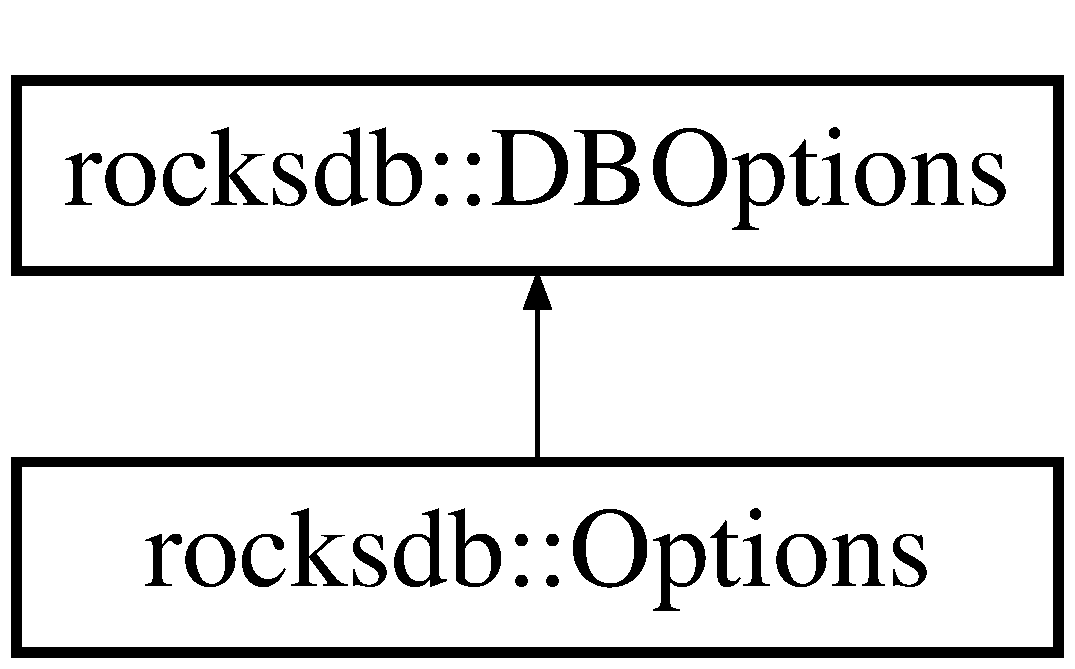
\includegraphics[height=2.000000cm]{structrocksdb_1_1DBOptions}
\end{center}
\end{figure}
\subsection*{Public Types}
\begin{DoxyCompactItemize}
\item 
enum {\bfseries Access\+Hint} \{ {\bfseries N\+O\+NE}, 
{\bfseries N\+O\+R\+M\+AL}, 
{\bfseries S\+E\+Q\+U\+E\+N\+T\+I\+AL}, 
{\bfseries W\+I\+L\+L\+N\+E\+ED}
 \}\hypertarget{structrocksdb_1_1DBOptions_a4c0ee6860de664497ef1da15d1df2f11}{}\label{structrocksdb_1_1DBOptions_a4c0ee6860de664497ef1da15d1df2f11}

\end{DoxyCompactItemize}
\subsection*{Public Member Functions}
\begin{DoxyCompactItemize}
\item 
\hyperlink{structrocksdb_1_1DBOptions}{D\+B\+Options} $\ast$ {\bfseries Old\+Defaults} (int rocksdb\+\_\+major\+\_\+version=4, int rocksdb\+\_\+minor\+\_\+version=6)\hypertarget{structrocksdb_1_1DBOptions_a5a227d520fc66dd3836a69fe32e225e8}{}\label{structrocksdb_1_1DBOptions_a5a227d520fc66dd3836a69fe32e225e8}

\item 
\hyperlink{structrocksdb_1_1DBOptions}{D\+B\+Options} $\ast$ {\bfseries Increase\+Parallelism} (int total\+\_\+threads=16)\hypertarget{structrocksdb_1_1DBOptions_ab0db4bd149b283e652862784715da0d6}{}\label{structrocksdb_1_1DBOptions_ab0db4bd149b283e652862784715da0d6}

\item 
{\bfseries D\+B\+Options} (const \hyperlink{structrocksdb_1_1Options}{Options} \&options)\hypertarget{structrocksdb_1_1DBOptions_a75ada8388a24596c5e4aa1bc9bac4b39}{}\label{structrocksdb_1_1DBOptions_a75ada8388a24596c5e4aa1bc9bac4b39}

\item 
void {\bfseries Dump} (\hyperlink{classrocksdb_1_1Logger}{Logger} $\ast$log) const\hypertarget{structrocksdb_1_1DBOptions_a8068fb42d793c7a567bc44e5aed50844}{}\label{structrocksdb_1_1DBOptions_a8068fb42d793c7a567bc44e5aed50844}

\end{DoxyCompactItemize}
\subsection*{Public Attributes}
\begin{DoxyCompactItemize}
\item 
bool {\bfseries create\+\_\+if\+\_\+missing}\hypertarget{structrocksdb_1_1DBOptions_abdcf05ab83219edf0d03d8d02d39ee0c}{}\label{structrocksdb_1_1DBOptions_abdcf05ab83219edf0d03d8d02d39ee0c}

\item 
bool {\bfseries create\+\_\+missing\+\_\+column\+\_\+families}\hypertarget{structrocksdb_1_1DBOptions_a4d8d13c5e43ca4a5b2a54f08aa3b7f60}{}\label{structrocksdb_1_1DBOptions_a4d8d13c5e43ca4a5b2a54f08aa3b7f60}

\item 
bool {\bfseries error\+\_\+if\+\_\+exists}\hypertarget{structrocksdb_1_1DBOptions_a4487e7de36b93dc5a06d6daf21bac151}{}\label{structrocksdb_1_1DBOptions_a4487e7de36b93dc5a06d6daf21bac151}

\item 
bool {\bfseries paranoid\+\_\+checks}\hypertarget{structrocksdb_1_1DBOptions_a0797bb6a87fc0345f24330ad531977c7}{}\label{structrocksdb_1_1DBOptions_a0797bb6a87fc0345f24330ad531977c7}

\item 
\hyperlink{classrocksdb_1_1Env}{Env} $\ast$ {\bfseries env}\hypertarget{structrocksdb_1_1DBOptions_a5c6e3419dd7cad2e73f746a5a5975ff9}{}\label{structrocksdb_1_1DBOptions_a5c6e3419dd7cad2e73f746a5a5975ff9}

\item 
std\+::shared\+\_\+ptr$<$ \hyperlink{classrocksdb_1_1RateLimiter}{Rate\+Limiter} $>$ {\bfseries rate\+\_\+limiter}\hypertarget{structrocksdb_1_1DBOptions_aede14b809742935900cd5a8b544ad7b3}{}\label{structrocksdb_1_1DBOptions_aede14b809742935900cd5a8b544ad7b3}

\item 
std\+::shared\+\_\+ptr$<$ \hyperlink{classrocksdb_1_1SstFileManager}{Sst\+File\+Manager} $>$ {\bfseries sst\+\_\+file\+\_\+manager}\hypertarget{structrocksdb_1_1DBOptions_a138d954e6c0b69672c7a9eaf7ad11d3f}{}\label{structrocksdb_1_1DBOptions_a138d954e6c0b69672c7a9eaf7ad11d3f}

\item 
std\+::shared\+\_\+ptr$<$ \hyperlink{classrocksdb_1_1Logger}{Logger} $>$ {\bfseries info\+\_\+log}\hypertarget{structrocksdb_1_1DBOptions_ac7eb66ab129bde4525879c737435c98e}{}\label{structrocksdb_1_1DBOptions_ac7eb66ab129bde4525879c737435c98e}

\item 
Info\+Log\+Level {\bfseries info\+\_\+log\+\_\+level}\hypertarget{structrocksdb_1_1DBOptions_a1570666f5bea2ae94bac7b2dd654cdce}{}\label{structrocksdb_1_1DBOptions_a1570666f5bea2ae94bac7b2dd654cdce}

\item 
int {\bfseries max\+\_\+open\+\_\+files}\hypertarget{structrocksdb_1_1DBOptions_a53adcfcc54693af498dffc659d39483f}{}\label{structrocksdb_1_1DBOptions_a53adcfcc54693af498dffc659d39483f}

\item 
int {\bfseries max\+\_\+file\+\_\+opening\+\_\+threads}\hypertarget{structrocksdb_1_1DBOptions_a6420806df488a43d450b7b8716f3544a}{}\label{structrocksdb_1_1DBOptions_a6420806df488a43d450b7b8716f3544a}

\item 
uint64\+\_\+t {\bfseries max\+\_\+total\+\_\+wal\+\_\+size}\hypertarget{structrocksdb_1_1DBOptions_a1e2d3510fc4b1ace1c1f1164ec9e3719}{}\label{structrocksdb_1_1DBOptions_a1e2d3510fc4b1ace1c1f1164ec9e3719}

\item 
std\+::shared\+\_\+ptr$<$ \hyperlink{classrocksdb_1_1Statistics}{Statistics} $>$ {\bfseries statistics}\hypertarget{structrocksdb_1_1DBOptions_a9662869d64a51af1e2ebbf3c9085c927}{}\label{structrocksdb_1_1DBOptions_a9662869d64a51af1e2ebbf3c9085c927}

\item 
bool {\bfseries disable\+Data\+Sync}\hypertarget{structrocksdb_1_1DBOptions_aedd20f6079fab3fb4e86e661c730325f}{}\label{structrocksdb_1_1DBOptions_aedd20f6079fab3fb4e86e661c730325f}

\item 
bool {\bfseries use\+\_\+fsync}\hypertarget{structrocksdb_1_1DBOptions_a5185be98a0135dbbedd2495b3f5e0311}{}\label{structrocksdb_1_1DBOptions_a5185be98a0135dbbedd2495b3f5e0311}

\item 
std\+::vector$<$ \hyperlink{structrocksdb_1_1DbPath}{Db\+Path} $>$ {\bfseries db\+\_\+paths}\hypertarget{structrocksdb_1_1DBOptions_af781d0124975adecfdfa615be0dfd2ea}{}\label{structrocksdb_1_1DBOptions_af781d0124975adecfdfa615be0dfd2ea}

\item 
std\+::string {\bfseries db\+\_\+log\+\_\+dir}\hypertarget{structrocksdb_1_1DBOptions_aa1b533683a34bf2e9d4380e568ba6c8a}{}\label{structrocksdb_1_1DBOptions_aa1b533683a34bf2e9d4380e568ba6c8a}

\item 
std\+::string {\bfseries wal\+\_\+dir}\hypertarget{structrocksdb_1_1DBOptions_a384cdc01f0f2906930144381b93de2e0}{}\label{structrocksdb_1_1DBOptions_a384cdc01f0f2906930144381b93de2e0}

\item 
uint64\+\_\+t {\bfseries delete\+\_\+obsolete\+\_\+files\+\_\+period\+\_\+micros}\hypertarget{structrocksdb_1_1DBOptions_a9bad65d02bd2049d30b45599ef8c35bb}{}\label{structrocksdb_1_1DBOptions_a9bad65d02bd2049d30b45599ef8c35bb}

\item 
int {\bfseries base\+\_\+background\+\_\+compactions}\hypertarget{structrocksdb_1_1DBOptions_ace75f288ddb9afa9a81d53b1eff96b43}{}\label{structrocksdb_1_1DBOptions_ace75f288ddb9afa9a81d53b1eff96b43}

\item 
int {\bfseries max\+\_\+background\+\_\+compactions}\hypertarget{structrocksdb_1_1DBOptions_adc51fcd7138149a50ef57bf146aaaae3}{}\label{structrocksdb_1_1DBOptions_adc51fcd7138149a50ef57bf146aaaae3}

\item 
uint32\+\_\+t {\bfseries max\+\_\+subcompactions}\hypertarget{structrocksdb_1_1DBOptions_a870b445c2d1222939a4367a58a775574}{}\label{structrocksdb_1_1DBOptions_a870b445c2d1222939a4367a58a775574}

\item 
int {\bfseries max\+\_\+background\+\_\+flushes}\hypertarget{structrocksdb_1_1DBOptions_af0deda157b0ecb70121239429e55f548}{}\label{structrocksdb_1_1DBOptions_af0deda157b0ecb70121239429e55f548}

\item 
size\+\_\+t {\bfseries max\+\_\+log\+\_\+file\+\_\+size}\hypertarget{structrocksdb_1_1DBOptions_a091e003256873b2c5b23b9dbd4f0598b}{}\label{structrocksdb_1_1DBOptions_a091e003256873b2c5b23b9dbd4f0598b}

\item 
size\+\_\+t {\bfseries log\+\_\+file\+\_\+time\+\_\+to\+\_\+roll}\hypertarget{structrocksdb_1_1DBOptions_afa52da87a90d2453fe3c43a8fb2ea126}{}\label{structrocksdb_1_1DBOptions_afa52da87a90d2453fe3c43a8fb2ea126}

\item 
size\+\_\+t {\bfseries keep\+\_\+log\+\_\+file\+\_\+num}\hypertarget{structrocksdb_1_1DBOptions_ade2727a3b6e9b9a410ec2d5f3810a1a9}{}\label{structrocksdb_1_1DBOptions_ade2727a3b6e9b9a410ec2d5f3810a1a9}

\item 
size\+\_\+t {\bfseries recycle\+\_\+log\+\_\+file\+\_\+num}\hypertarget{structrocksdb_1_1DBOptions_a546aa687572f9d68f75d3918b527fe7e}{}\label{structrocksdb_1_1DBOptions_a546aa687572f9d68f75d3918b527fe7e}

\item 
uint64\+\_\+t {\bfseries max\+\_\+manifest\+\_\+file\+\_\+size}\hypertarget{structrocksdb_1_1DBOptions_a7966751f8a167645900fe6307a4abe80}{}\label{structrocksdb_1_1DBOptions_a7966751f8a167645900fe6307a4abe80}

\item 
int {\bfseries table\+\_\+cache\+\_\+numshardbits}\hypertarget{structrocksdb_1_1DBOptions_a4411b1598a56ad2f4525cd59cb864ccf}{}\label{structrocksdb_1_1DBOptions_a4411b1598a56ad2f4525cd59cb864ccf}

\item 
uint64\+\_\+t {\bfseries W\+A\+L\+\_\+ttl\+\_\+seconds}\hypertarget{structrocksdb_1_1DBOptions_a516d9f0c5aec8397be3986b2c9e4db0f}{}\label{structrocksdb_1_1DBOptions_a516d9f0c5aec8397be3986b2c9e4db0f}

\item 
uint64\+\_\+t {\bfseries W\+A\+L\+\_\+size\+\_\+limit\+\_\+\+MB}\hypertarget{structrocksdb_1_1DBOptions_a04f4ffed6308ac8c59cbf5f916ee09cf}{}\label{structrocksdb_1_1DBOptions_a04f4ffed6308ac8c59cbf5f916ee09cf}

\item 
size\+\_\+t {\bfseries manifest\+\_\+preallocation\+\_\+size}\hypertarget{structrocksdb_1_1DBOptions_af7a3815f4c1809b18f0ebea46227ec8d}{}\label{structrocksdb_1_1DBOptions_af7a3815f4c1809b18f0ebea46227ec8d}

\item 
bool {\bfseries allow\+\_\+os\+\_\+buffer}\hypertarget{structrocksdb_1_1DBOptions_ac17d6620171a35f095846d23c06d5077}{}\label{structrocksdb_1_1DBOptions_ac17d6620171a35f095846d23c06d5077}

\item 
bool {\bfseries allow\+\_\+mmap\+\_\+reads}\hypertarget{structrocksdb_1_1DBOptions_a407f41b438848143b00a05445f69d453}{}\label{structrocksdb_1_1DBOptions_a407f41b438848143b00a05445f69d453}

\item 
bool {\bfseries allow\+\_\+mmap\+\_\+writes}\hypertarget{structrocksdb_1_1DBOptions_a55616ba06da6f436df7f3ff90471aa81}{}\label{structrocksdb_1_1DBOptions_a55616ba06da6f436df7f3ff90471aa81}

\item 
bool {\bfseries allow\+\_\+fallocate}\hypertarget{structrocksdb_1_1DBOptions_a81d82bc783905db0be041bd12bb7b78c}{}\label{structrocksdb_1_1DBOptions_a81d82bc783905db0be041bd12bb7b78c}

\item 
bool {\bfseries is\+\_\+fd\+\_\+close\+\_\+on\+\_\+exec}\hypertarget{structrocksdb_1_1DBOptions_acf446290a9583f2cab95ca1474c34283}{}\label{structrocksdb_1_1DBOptions_acf446290a9583f2cab95ca1474c34283}

\item 
bool {\bfseries skip\+\_\+log\+\_\+error\+\_\+on\+\_\+recovery}\hypertarget{structrocksdb_1_1DBOptions_aec1622bde76ec56c47bae87fb19e479d}{}\label{structrocksdb_1_1DBOptions_aec1622bde76ec56c47bae87fb19e479d}

\item 
unsigned int {\bfseries stats\+\_\+dump\+\_\+period\+\_\+sec}\hypertarget{structrocksdb_1_1DBOptions_a004866a30f79640d98c646c2b248a372}{}\label{structrocksdb_1_1DBOptions_a004866a30f79640d98c646c2b248a372}

\item 
bool {\bfseries advise\+\_\+random\+\_\+on\+\_\+open}\hypertarget{structrocksdb_1_1DBOptions_ab8a7b88f235cf5745b073ea2d799aab5}{}\label{structrocksdb_1_1DBOptions_ab8a7b88f235cf5745b073ea2d799aab5}

\item 
size\+\_\+t {\bfseries db\+\_\+write\+\_\+buffer\+\_\+size}\hypertarget{structrocksdb_1_1DBOptions_af1542493f100003fb3a1de29d6c37f69}{}\label{structrocksdb_1_1DBOptions_af1542493f100003fb3a1de29d6c37f69}

\item 
Access\+Hint {\bfseries access\+\_\+hint\+\_\+on\+\_\+compaction\+\_\+start}\hypertarget{structrocksdb_1_1DBOptions_a6be9d7a11b2050d11a709e9db0147d8e}{}\label{structrocksdb_1_1DBOptions_a6be9d7a11b2050d11a709e9db0147d8e}

\item 
bool {\bfseries new\+\_\+table\+\_\+reader\+\_\+for\+\_\+compaction\+\_\+inputs}\hypertarget{structrocksdb_1_1DBOptions_a528c773705773c219406a38866d1add8}{}\label{structrocksdb_1_1DBOptions_a528c773705773c219406a38866d1add8}

\item 
size\+\_\+t {\bfseries compaction\+\_\+readahead\+\_\+size}\hypertarget{structrocksdb_1_1DBOptions_abae810e6352793500cb748a970248836}{}\label{structrocksdb_1_1DBOptions_abae810e6352793500cb748a970248836}

\item 
size\+\_\+t {\bfseries random\+\_\+access\+\_\+max\+\_\+buffer\+\_\+size}\hypertarget{structrocksdb_1_1DBOptions_ace1cce7e8f1cfe2b12247bdb8751ce2a}{}\label{structrocksdb_1_1DBOptions_ace1cce7e8f1cfe2b12247bdb8751ce2a}

\item 
size\+\_\+t {\bfseries writable\+\_\+file\+\_\+max\+\_\+buffer\+\_\+size}\hypertarget{structrocksdb_1_1DBOptions_a4c4efda9615704dc07bc278957e33c16}{}\label{structrocksdb_1_1DBOptions_a4c4efda9615704dc07bc278957e33c16}

\item 
bool {\bfseries use\+\_\+adaptive\+\_\+mutex}\hypertarget{structrocksdb_1_1DBOptions_ad9819f8645d0529285b0845545cd9286}{}\label{structrocksdb_1_1DBOptions_ad9819f8645d0529285b0845545cd9286}

\item 
uint64\+\_\+t {\bfseries bytes\+\_\+per\+\_\+sync}\hypertarget{structrocksdb_1_1DBOptions_a906e2c4dc27261d6c38761b32fc327bc}{}\label{structrocksdb_1_1DBOptions_a906e2c4dc27261d6c38761b32fc327bc}

\item 
uint64\+\_\+t {\bfseries wal\+\_\+bytes\+\_\+per\+\_\+sync}\hypertarget{structrocksdb_1_1DBOptions_a651aad787c4a3692e504720f46a560ed}{}\label{structrocksdb_1_1DBOptions_a651aad787c4a3692e504720f46a560ed}

\item 
std\+::vector$<$ std\+::shared\+\_\+ptr$<$ \hyperlink{classrocksdb_1_1EventListener}{Event\+Listener} $>$ $>$ {\bfseries listeners}\hypertarget{structrocksdb_1_1DBOptions_a181c95f50c27dc35683e51dfdbe6fb23}{}\label{structrocksdb_1_1DBOptions_a181c95f50c27dc35683e51dfdbe6fb23}

\item 
bool {\bfseries enable\+\_\+thread\+\_\+tracking}\hypertarget{structrocksdb_1_1DBOptions_a363866053585683ad59e218da91da55b}{}\label{structrocksdb_1_1DBOptions_a363866053585683ad59e218da91da55b}

\item 
uint64\+\_\+t {\bfseries delayed\+\_\+write\+\_\+rate}\hypertarget{structrocksdb_1_1DBOptions_a0be34d0f483e371cfdfd5eacb916e3d9}{}\label{structrocksdb_1_1DBOptions_a0be34d0f483e371cfdfd5eacb916e3d9}

\item 
bool {\bfseries allow\+\_\+concurrent\+\_\+memtable\+\_\+write}\hypertarget{structrocksdb_1_1DBOptions_ae2ae762f46b856a815e852d7ba296a59}{}\label{structrocksdb_1_1DBOptions_ae2ae762f46b856a815e852d7ba296a59}

\item 
bool {\bfseries enable\+\_\+write\+\_\+thread\+\_\+adaptive\+\_\+yield}\hypertarget{structrocksdb_1_1DBOptions_aeb3dc073acbd119db542100a9f3666b5}{}\label{structrocksdb_1_1DBOptions_aeb3dc073acbd119db542100a9f3666b5}

\item 
uint64\+\_\+t {\bfseries write\+\_\+thread\+\_\+max\+\_\+yield\+\_\+usec}\hypertarget{structrocksdb_1_1DBOptions_ab1d40797f52ec7ad0a822af8559833ce}{}\label{structrocksdb_1_1DBOptions_ab1d40797f52ec7ad0a822af8559833ce}

\item 
uint64\+\_\+t {\bfseries write\+\_\+thread\+\_\+slow\+\_\+yield\+\_\+usec}\hypertarget{structrocksdb_1_1DBOptions_aa6bdd335a0bd7a1b335505faf31935f4}{}\label{structrocksdb_1_1DBOptions_aa6bdd335a0bd7a1b335505faf31935f4}

\item 
bool {\bfseries skip\+\_\+stats\+\_\+update\+\_\+on\+\_\+db\+\_\+open}\hypertarget{structrocksdb_1_1DBOptions_a019b1f46fb8a5f97b5e291ca33e8da5e}{}\label{structrocksdb_1_1DBOptions_a019b1f46fb8a5f97b5e291ca33e8da5e}

\item 
W\+A\+L\+Recovery\+Mode {\bfseries wal\+\_\+recovery\+\_\+mode}\hypertarget{structrocksdb_1_1DBOptions_af967c466aa612c9e5a777b44944653dc}{}\label{structrocksdb_1_1DBOptions_af967c466aa612c9e5a777b44944653dc}

\item 
std\+::shared\+\_\+ptr$<$ \hyperlink{classrocksdb_1_1Cache}{Cache} $>$ {\bfseries row\+\_\+cache}\hypertarget{structrocksdb_1_1DBOptions_ac272dc7a8a93351a7494ccfd128cac5a}{}\label{structrocksdb_1_1DBOptions_ac272dc7a8a93351a7494ccfd128cac5a}

\item 
\hyperlink{classrocksdb_1_1WalFilter}{Wal\+Filter} $\ast$ {\bfseries wal\+\_\+filter}\hypertarget{structrocksdb_1_1DBOptions_ad4a27b9f67d3c1f03fe77a09c26608ad}{}\label{structrocksdb_1_1DBOptions_ad4a27b9f67d3c1f03fe77a09c26608ad}

\item 
bool {\bfseries fail\+\_\+if\+\_\+options\+\_\+file\+\_\+error}\hypertarget{structrocksdb_1_1DBOptions_aa50efc7702bd62de3e8096d1afc9cdb4}{}\label{structrocksdb_1_1DBOptions_aa50efc7702bd62de3e8096d1afc9cdb4}

\end{DoxyCompactItemize}


The documentation for this struct was generated from the following file\+:\begin{DoxyCompactItemize}
\item 
Appserver/src/external/rocksdb/options.\+h\end{DoxyCompactItemize}

\hypertarget{structrocksdb_1_1DbPath}{}\section{rocksdb\+:\+:Db\+Path Struct Reference}
\label{structrocksdb_1_1DbPath}\index{rocksdb\+::\+Db\+Path@{rocksdb\+::\+Db\+Path}}
\subsection*{Public Member Functions}
\begin{DoxyCompactItemize}
\item 
{\bfseries Db\+Path} (const std\+::string \&p, uint64\+\_\+t t)\hypertarget{structrocksdb_1_1DbPath_a6e982ec78af59710f41c59bd06801a7c}{}\label{structrocksdb_1_1DbPath_a6e982ec78af59710f41c59bd06801a7c}

\end{DoxyCompactItemize}
\subsection*{Public Attributes}
\begin{DoxyCompactItemize}
\item 
std\+::string {\bfseries path}\hypertarget{structrocksdb_1_1DbPath_a010b8c715e856b33a9bc8351b096f62d}{}\label{structrocksdb_1_1DbPath_a010b8c715e856b33a9bc8351b096f62d}

\item 
uint64\+\_\+t {\bfseries target\+\_\+size}\hypertarget{structrocksdb_1_1DbPath_aaef4845c332e0fb7ee46ca8fc4917786}{}\label{structrocksdb_1_1DbPath_aaef4845c332e0fb7ee46ca8fc4917786}

\end{DoxyCompactItemize}


The documentation for this struct was generated from the following file\+:\begin{DoxyCompactItemize}
\item 
Appserver/src/external/rocksdb/options.\+h\end{DoxyCompactItemize}

\hypertarget{classrocksdb_1_1DbUndumpTool}{}\section{rocksdb\+:\+:Db\+Undump\+Tool Class Reference}
\label{classrocksdb_1_1DbUndumpTool}\index{rocksdb\+::\+Db\+Undump\+Tool@{rocksdb\+::\+Db\+Undump\+Tool}}
\subsection*{Public Member Functions}
\begin{DoxyCompactItemize}
\item 
bool {\bfseries Run} (const \hyperlink{structrocksdb_1_1UndumpOptions}{Undump\+Options} \&undump\+\_\+options, \hyperlink{structrocksdb_1_1Options}{rocksdb\+::\+Options} options=\hyperlink{structrocksdb_1_1Options}{rocksdb\+::\+Options}())\hypertarget{classrocksdb_1_1DbUndumpTool_a1572278b116102bbb139c3da6dc3e3b2}{}\label{classrocksdb_1_1DbUndumpTool_a1572278b116102bbb139c3da6dc3e3b2}

\end{DoxyCompactItemize}


The documentation for this class was generated from the following file\+:\begin{DoxyCompactItemize}
\item 
Appserver/src/external/rocksdb/db\+\_\+dump\+\_\+tool.\+h\end{DoxyCompactItemize}

\hypertarget{classrocksdb_1_1DBWithTTL}{}\section{rocksdb\+:\+:D\+B\+With\+T\+TL Class Reference}
\label{classrocksdb_1_1DBWithTTL}\index{rocksdb\+::\+D\+B\+With\+T\+TL@{rocksdb\+::\+D\+B\+With\+T\+TL}}
Inheritance diagram for rocksdb\+:\+:D\+B\+With\+T\+TL\+:\begin{figure}[H]
\begin{center}
\leavevmode
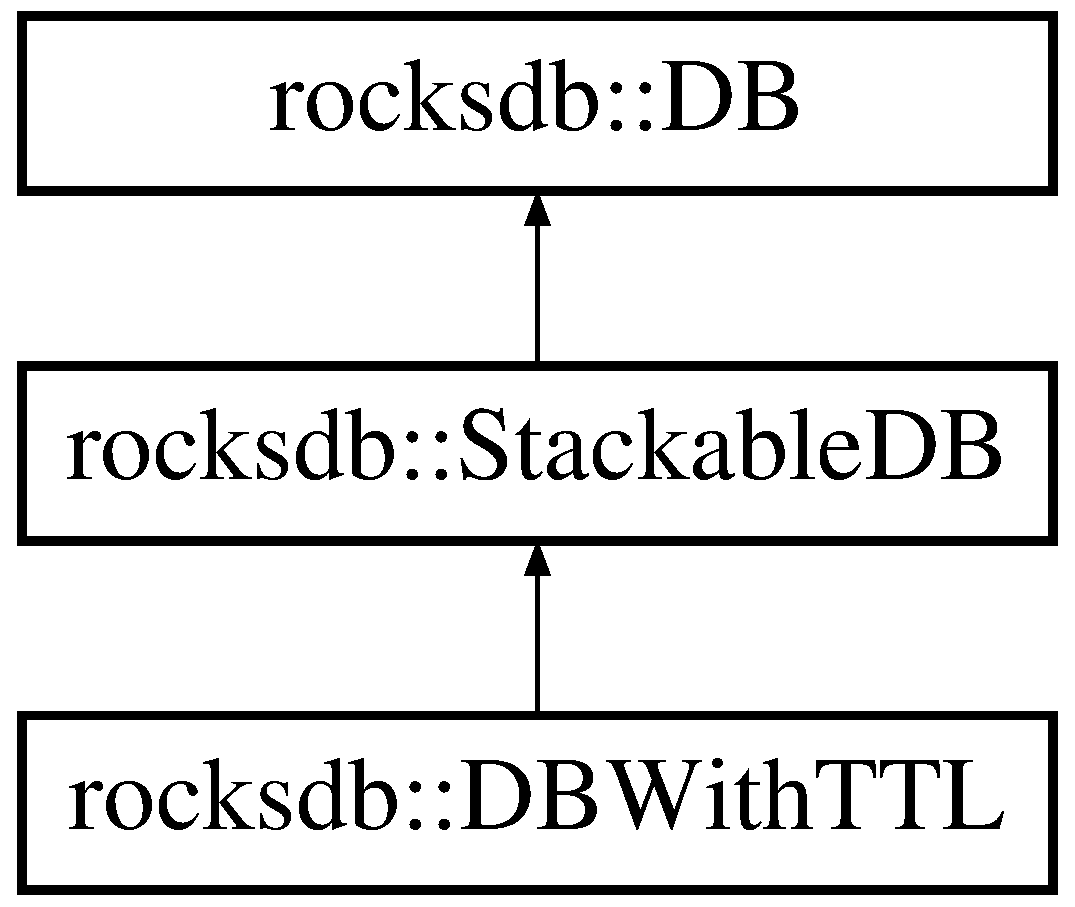
\includegraphics[height=3.000000cm]{classrocksdb_1_1DBWithTTL}
\end{center}
\end{figure}
\subsection*{Public Member Functions}
\begin{DoxyCompactItemize}
\item 
virtual \hyperlink{classrocksdb_1_1Status}{Status} {\bfseries Create\+Column\+Family\+With\+Ttl} (const \hyperlink{structrocksdb_1_1ColumnFamilyOptions}{Column\+Family\+Options} \&options, const std\+::string \&column\+\_\+family\+\_\+name, \hyperlink{classrocksdb_1_1ColumnFamilyHandle}{Column\+Family\+Handle} $\ast$$\ast$handle, int ttl)=0\hypertarget{classrocksdb_1_1DBWithTTL_a97b67542889448b90229760b352bac20}{}\label{classrocksdb_1_1DBWithTTL_a97b67542889448b90229760b352bac20}

\end{DoxyCompactItemize}
\subsection*{Static Public Member Functions}
\begin{DoxyCompactItemize}
\item 
static \hyperlink{classrocksdb_1_1Status}{Status} {\bfseries Open} (const \hyperlink{structrocksdb_1_1Options}{Options} \&options, const std\+::string \&dbname, \hyperlink{classrocksdb_1_1DBWithTTL}{D\+B\+With\+T\+TL} $\ast$$\ast$dbptr, int32\+\_\+t ttl=0, bool read\+\_\+only=false)\hypertarget{classrocksdb_1_1DBWithTTL_a8a87051b59fb482779912dc1a91a7b5d}{}\label{classrocksdb_1_1DBWithTTL_a8a87051b59fb482779912dc1a91a7b5d}

\item 
static \hyperlink{classrocksdb_1_1Status}{Status} {\bfseries Open} (const \hyperlink{structrocksdb_1_1DBOptions}{D\+B\+Options} \&db\+\_\+options, const std\+::string \&dbname, const std\+::vector$<$ \hyperlink{structrocksdb_1_1ColumnFamilyDescriptor}{Column\+Family\+Descriptor} $>$ \&column\+\_\+families, std\+::vector$<$ \hyperlink{classrocksdb_1_1ColumnFamilyHandle}{Column\+Family\+Handle} $\ast$$>$ $\ast$handles, \hyperlink{classrocksdb_1_1DBWithTTL}{D\+B\+With\+T\+TL} $\ast$$\ast$dbptr, std\+::vector$<$ int32\+\_\+t $>$ ttls, bool read\+\_\+only=false)\hypertarget{classrocksdb_1_1DBWithTTL_a932f8af06302d6358cf202ae47d93bd5}{}\label{classrocksdb_1_1DBWithTTL_a932f8af06302d6358cf202ae47d93bd5}

\end{DoxyCompactItemize}
\subsection*{Protected Member Functions}
\begin{DoxyCompactItemize}
\item 
{\bfseries D\+B\+With\+T\+TL} (\hyperlink{classrocksdb_1_1DB}{DB} $\ast$db)\hypertarget{classrocksdb_1_1DBWithTTL_a31f23bd0807fa7f60041aa768a80ee0d}{}\label{classrocksdb_1_1DBWithTTL_a31f23bd0807fa7f60041aa768a80ee0d}

\end{DoxyCompactItemize}
\subsection*{Additional Inherited Members}


The documentation for this class was generated from the following file\+:\begin{DoxyCompactItemize}
\item 
Appserver/src/external/rocksdb/utilities/db\+\_\+ttl.\+h\end{DoxyCompactItemize}

\hypertarget{classrocksdb_1_1Directory}{}\section{rocksdb\+:\+:Directory Class Reference}
\label{classrocksdb_1_1Directory}\index{rocksdb\+::\+Directory@{rocksdb\+::\+Directory}}
\subsection*{Public Member Functions}
\begin{DoxyCompactItemize}
\item 
virtual \hyperlink{classrocksdb_1_1Status}{Status} {\bfseries Fsync} ()=0\hypertarget{classrocksdb_1_1Directory_a1549af56279af088c832f3b7bcd8ea6e}{}\label{classrocksdb_1_1Directory_a1549af56279af088c832f3b7bcd8ea6e}

\end{DoxyCompactItemize}


The documentation for this class was generated from the following file\+:\begin{DoxyCompactItemize}
\item 
Appserver/src/external/rocksdb/env.\+h\end{DoxyCompactItemize}

\hypertarget{classrocksdb_1_1DocumentDB}{}\section{rocksdb\+:\+:Document\+DB Class Reference}
\label{classrocksdb_1_1DocumentDB}\index{rocksdb\+::\+Document\+DB@{rocksdb\+::\+Document\+DB}}
Inheritance diagram for rocksdb\+:\+:Document\+DB\+:\begin{figure}[H]
\begin{center}
\leavevmode
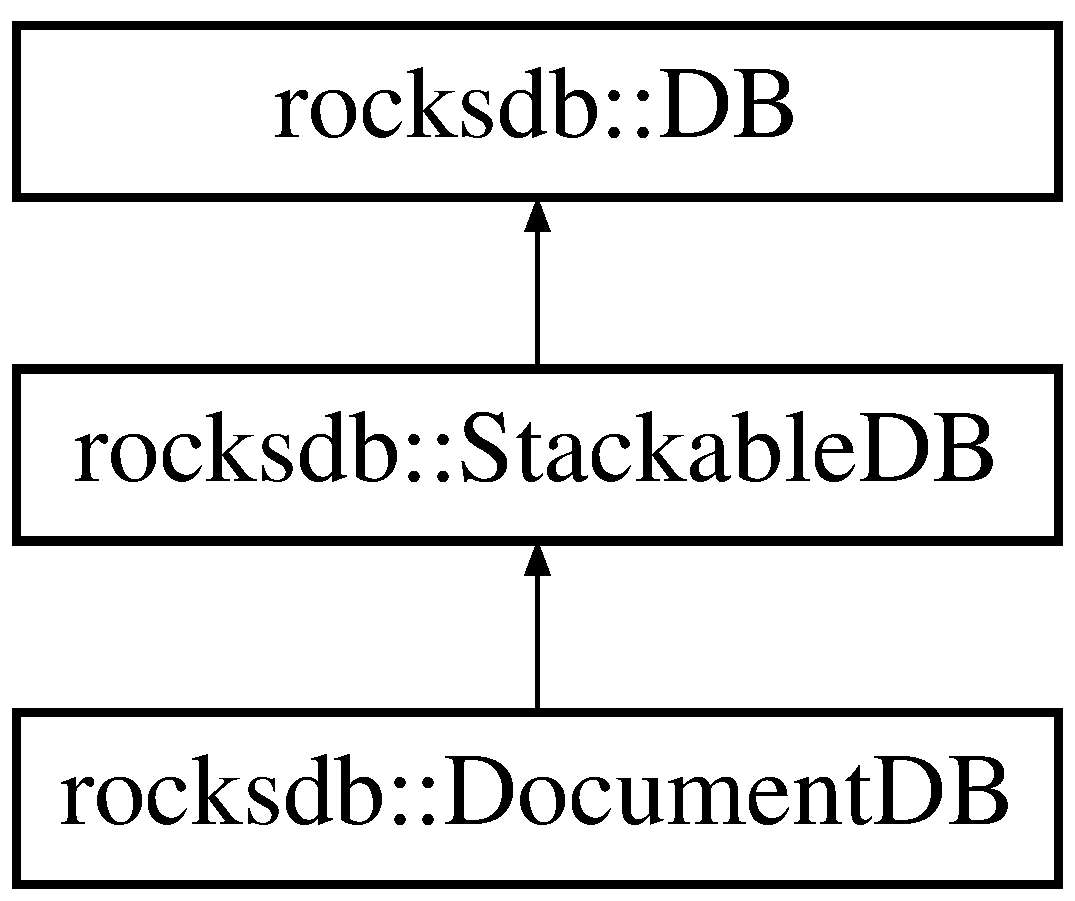
\includegraphics[height=3.000000cm]{classrocksdb_1_1DocumentDB}
\end{center}
\end{figure}
\subsection*{Classes}
\begin{DoxyCompactItemize}
\item 
struct \hyperlink{structrocksdb_1_1DocumentDB_1_1IndexDescriptor}{Index\+Descriptor}
\end{DoxyCompactItemize}
\subsection*{Public Member Functions}
\begin{DoxyCompactItemize}
\item 
{\bfseries Document\+DB} (\hyperlink{classrocksdb_1_1DB}{DB} $\ast$db)\hypertarget{classrocksdb_1_1DocumentDB_a7521c1576c8e97ac192be7a17856fe29}{}\label{classrocksdb_1_1DocumentDB_a7521c1576c8e97ac192be7a17856fe29}

\item 
virtual \hyperlink{classrocksdb_1_1Status}{Status} {\bfseries Create\+Index} (const \hyperlink{structrocksdb_1_1WriteOptions}{Write\+Options} \&write\+\_\+options, const \hyperlink{structrocksdb_1_1DocumentDB_1_1IndexDescriptor}{Index\+Descriptor} \&index)=0\hypertarget{classrocksdb_1_1DocumentDB_a3ba5420bc54b1016c62b491602ce3811}{}\label{classrocksdb_1_1DocumentDB_a3ba5420bc54b1016c62b491602ce3811}

\item 
virtual \hyperlink{classrocksdb_1_1Status}{Status} {\bfseries Drop\+Index} (const std\+::string \&name)=0\hypertarget{classrocksdb_1_1DocumentDB_a3f503331b6030566045f25bccd67209e}{}\label{classrocksdb_1_1DocumentDB_a3f503331b6030566045f25bccd67209e}

\item 
virtual \hyperlink{classrocksdb_1_1Status}{Status} {\bfseries Insert} (const \hyperlink{structrocksdb_1_1WriteOptions}{Write\+Options} \&options, const \hyperlink{classrocksdb_1_1JSONDocument}{J\+S\+O\+N\+Document} \&document)=0\hypertarget{classrocksdb_1_1DocumentDB_ac456af22d4bd0dad85476593af18a05a}{}\label{classrocksdb_1_1DocumentDB_ac456af22d4bd0dad85476593af18a05a}

\item 
virtual \hyperlink{classrocksdb_1_1Status}{Status} {\bfseries Remove} (const \hyperlink{structrocksdb_1_1ReadOptions}{Read\+Options} \&read\+\_\+options, const \hyperlink{structrocksdb_1_1WriteOptions}{Write\+Options} \&write\+\_\+options, const \hyperlink{classrocksdb_1_1JSONDocument}{J\+S\+O\+N\+Document} \&query)=0\hypertarget{classrocksdb_1_1DocumentDB_ac45f6bf1c1206f9307c106217a6fed3a}{}\label{classrocksdb_1_1DocumentDB_ac45f6bf1c1206f9307c106217a6fed3a}

\item 
virtual \hyperlink{classrocksdb_1_1Status}{Status} {\bfseries Update} (const \hyperlink{structrocksdb_1_1ReadOptions}{Read\+Options} \&read\+\_\+options, const \hyperlink{structrocksdb_1_1WriteOptions}{Write\+Options} \&write\+\_\+options, const \hyperlink{classrocksdb_1_1JSONDocument}{J\+S\+O\+N\+Document} \&filter, const \hyperlink{classrocksdb_1_1JSONDocument}{J\+S\+O\+N\+Document} \&updates)=0\hypertarget{classrocksdb_1_1DocumentDB_a433f73b4550bc683c4700b1d9c7625d5}{}\label{classrocksdb_1_1DocumentDB_a433f73b4550bc683c4700b1d9c7625d5}

\item 
virtual \hyperlink{classrocksdb_1_1Cursor}{Cursor} $\ast$ {\bfseries Query} (const \hyperlink{structrocksdb_1_1ReadOptions}{Read\+Options} \&read\+\_\+options, const \hyperlink{classrocksdb_1_1JSONDocument}{J\+S\+O\+N\+Document} \&query)=0\hypertarget{classrocksdb_1_1DocumentDB_a584dc4f0db8065f8d1c94563a80cd559}{}\label{classrocksdb_1_1DocumentDB_a584dc4f0db8065f8d1c94563a80cd559}

\end{DoxyCompactItemize}
\subsection*{Static Public Member Functions}
\begin{DoxyCompactItemize}
\item 
static \hyperlink{classrocksdb_1_1Status}{Status} {\bfseries Open} (const \hyperlink{structrocksdb_1_1DocumentDBOptions}{Document\+D\+B\+Options} \&options, const std\+::string \&name, const std\+::vector$<$ \hyperlink{structrocksdb_1_1DocumentDB_1_1IndexDescriptor}{Index\+Descriptor} $>$ \&indexes, \hyperlink{classrocksdb_1_1DocumentDB}{Document\+DB} $\ast$$\ast$db, bool read\+\_\+only=false)\hypertarget{classrocksdb_1_1DocumentDB_abd15334b981a303969cb16e6f152c69f}{}\label{classrocksdb_1_1DocumentDB_abd15334b981a303969cb16e6f152c69f}

\end{DoxyCompactItemize}
\subsection*{Additional Inherited Members}


The documentation for this class was generated from the following file\+:\begin{DoxyCompactItemize}
\item 
Appserver/src/external/rocksdb/utilities/document\+\_\+db.\+h\end{DoxyCompactItemize}

\hypertarget{structrocksdb_1_1DocumentDBOptions}{}\section{rocksdb\+:\+:Document\+D\+B\+Options Struct Reference}
\label{structrocksdb_1_1DocumentDBOptions}\index{rocksdb\+::\+Document\+D\+B\+Options@{rocksdb\+::\+Document\+D\+B\+Options}}
\subsection*{Public Attributes}
\begin{DoxyCompactItemize}
\item 
int {\bfseries background\+\_\+threads} = 4\hypertarget{structrocksdb_1_1DocumentDBOptions_a331eba3ecd8ad3d389ab380f352275ea}{}\label{structrocksdb_1_1DocumentDBOptions_a331eba3ecd8ad3d389ab380f352275ea}

\item 
uint64\+\_\+t {\bfseries memtable\+\_\+size} = 128 $\ast$ 1024 $\ast$ 1024\hypertarget{structrocksdb_1_1DocumentDBOptions_a1e67baa739b6f470790606ba1d86579e}{}\label{structrocksdb_1_1DocumentDBOptions_a1e67baa739b6f470790606ba1d86579e}

\item 
uint64\+\_\+t {\bfseries cache\+\_\+size} = 1 $\ast$ 1024 $\ast$ 1024 $\ast$ 1024\hypertarget{structrocksdb_1_1DocumentDBOptions_a967bc30f79f44d6d7cf1004513b6dd2d}{}\label{structrocksdb_1_1DocumentDBOptions_a967bc30f79f44d6d7cf1004513b6dd2d}

\end{DoxyCompactItemize}


The documentation for this struct was generated from the following file\+:\begin{DoxyCompactItemize}
\item 
Appserver/src/external/rocksdb/utilities/document\+\_\+db.\+h\end{DoxyCompactItemize}

\hypertarget{structrocksdb_1_1DumpOptions}{}\section{rocksdb\+:\+:Dump\+Options Struct Reference}
\label{structrocksdb_1_1DumpOptions}\index{rocksdb\+::\+Dump\+Options@{rocksdb\+::\+Dump\+Options}}
\subsection*{Public Attributes}
\begin{DoxyCompactItemize}
\item 
std\+::string {\bfseries db\+\_\+path}\hypertarget{structrocksdb_1_1DumpOptions_a72310b22f0d53835da17d63dedc9a8d5}{}\label{structrocksdb_1_1DumpOptions_a72310b22f0d53835da17d63dedc9a8d5}

\item 
std\+::string {\bfseries dump\+\_\+location}\hypertarget{structrocksdb_1_1DumpOptions_a44c9b1d8293560f56acfd9a317a3ff53}{}\label{structrocksdb_1_1DumpOptions_a44c9b1d8293560f56acfd9a317a3ff53}

\item 
bool {\bfseries anonymous} = false\hypertarget{structrocksdb_1_1DumpOptions_a7a770d37e506260e4603c745e602322d}{}\label{structrocksdb_1_1DumpOptions_a7a770d37e506260e4603c745e602322d}

\end{DoxyCompactItemize}


The documentation for this struct was generated from the following file\+:\begin{DoxyCompactItemize}
\item 
Appserver/src/external/rocksdb/db\+\_\+dump\+\_\+tool.\+h\end{DoxyCompactItemize}

\hypertarget{classrocksdb_1_1Env}{}\section{rocksdb\+:\+:Env Class Reference}
\label{classrocksdb_1_1Env}\index{rocksdb\+::\+Env@{rocksdb\+::\+Env}}
Inheritance diagram for rocksdb\+:\+:Env\+:\begin{figure}[H]
\begin{center}
\leavevmode
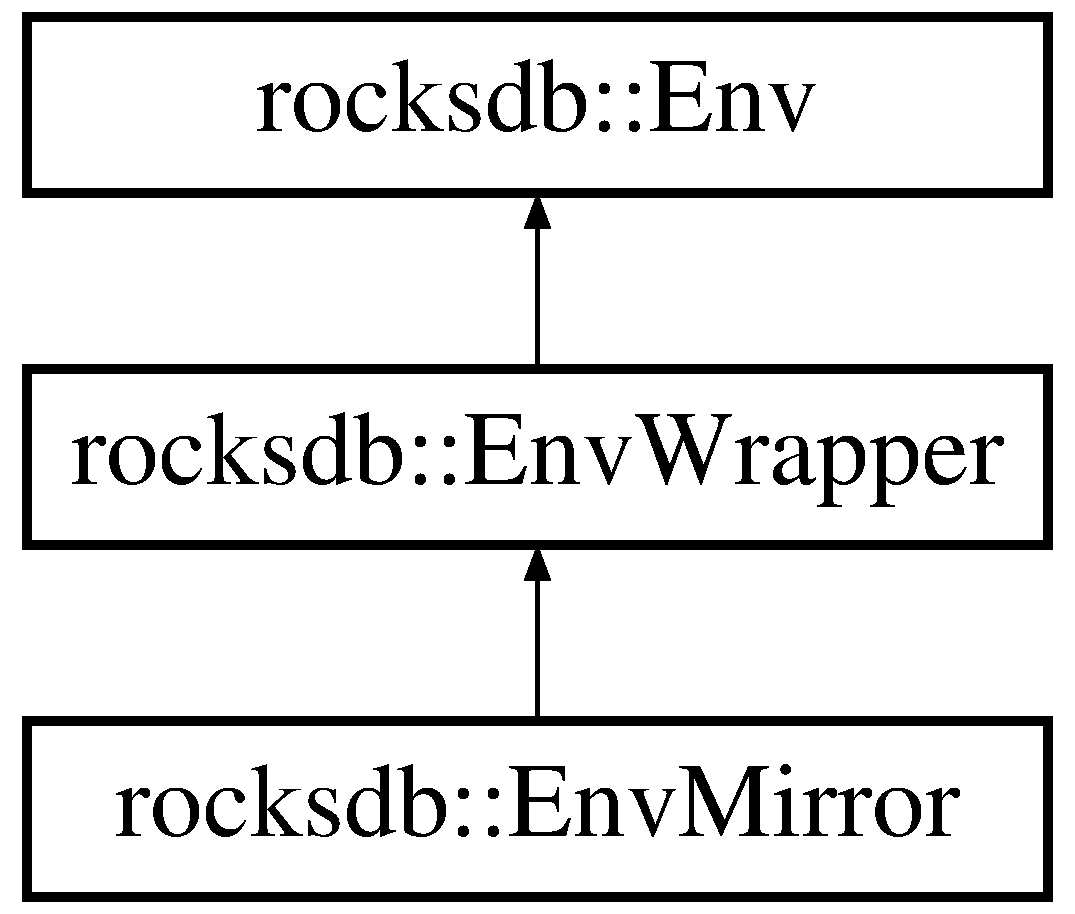
\includegraphics[height=3.000000cm]{classrocksdb_1_1Env}
\end{center}
\end{figure}
\subsection*{Classes}
\begin{DoxyCompactItemize}
\item 
struct \hyperlink{structrocksdb_1_1Env_1_1FileAttributes}{File\+Attributes}
\end{DoxyCompactItemize}
\subsection*{Public Types}
\begin{DoxyCompactItemize}
\item 
enum {\bfseries Priority} \{ {\bfseries L\+OW}, 
{\bfseries H\+I\+GH}, 
{\bfseries T\+O\+T\+AL}
 \}\hypertarget{classrocksdb_1_1Env_aa5be3083441b804767a9d554d7effcda}{}\label{classrocksdb_1_1Env_aa5be3083441b804767a9d554d7effcda}

\item 
enum {\bfseries I\+O\+Priority} \{ {\bfseries I\+O\+\_\+\+L\+OW} = 0, 
{\bfseries I\+O\+\_\+\+H\+I\+GH} = 1, 
{\bfseries I\+O\+\_\+\+T\+O\+T\+AL} = 2
 \}\hypertarget{classrocksdb_1_1Env_a20ebe3b9e9fae566e83e91249a02b021}{}\label{classrocksdb_1_1Env_a20ebe3b9e9fae566e83e91249a02b021}

\end{DoxyCompactItemize}
\subsection*{Public Member Functions}
\begin{DoxyCompactItemize}
\item 
virtual \hyperlink{classrocksdb_1_1Status}{Status} {\bfseries New\+Sequential\+File} (const std\+::string \&fname, unique\+\_\+ptr$<$ \hyperlink{classrocksdb_1_1SequentialFile}{Sequential\+File} $>$ $\ast$result, const \hyperlink{structrocksdb_1_1EnvOptions}{Env\+Options} \&options)=0\hypertarget{classrocksdb_1_1Env_af2eb6650bd551549c4f6f66ce0e51de3}{}\label{classrocksdb_1_1Env_af2eb6650bd551549c4f6f66ce0e51de3}

\item 
virtual \hyperlink{classrocksdb_1_1Status}{Status} {\bfseries New\+Random\+Access\+File} (const std\+::string \&fname, unique\+\_\+ptr$<$ \hyperlink{classrocksdb_1_1RandomAccessFile}{Random\+Access\+File} $>$ $\ast$result, const \hyperlink{structrocksdb_1_1EnvOptions}{Env\+Options} \&options)=0\hypertarget{classrocksdb_1_1Env_a6e6619074ecb6b5ba4e4a23ffb2e4974}{}\label{classrocksdb_1_1Env_a6e6619074ecb6b5ba4e4a23ffb2e4974}

\item 
virtual \hyperlink{classrocksdb_1_1Status}{Status} {\bfseries New\+Writable\+File} (const std\+::string \&fname, unique\+\_\+ptr$<$ \hyperlink{classrocksdb_1_1WritableFile}{Writable\+File} $>$ $\ast$result, const \hyperlink{structrocksdb_1_1EnvOptions}{Env\+Options} \&options)=0\hypertarget{classrocksdb_1_1Env_a2415186e0a399d70edabef9f477e4c47}{}\label{classrocksdb_1_1Env_a2415186e0a399d70edabef9f477e4c47}

\item 
virtual \hyperlink{classrocksdb_1_1Status}{Status} {\bfseries Reuse\+Writable\+File} (const std\+::string \&fname, const std\+::string \&old\+\_\+fname, unique\+\_\+ptr$<$ \hyperlink{classrocksdb_1_1WritableFile}{Writable\+File} $>$ $\ast$result, const \hyperlink{structrocksdb_1_1EnvOptions}{Env\+Options} \&options)\hypertarget{classrocksdb_1_1Env_abdb061a41cfd7f6d5ac57beb95f5aabc}{}\label{classrocksdb_1_1Env_abdb061a41cfd7f6d5ac57beb95f5aabc}

\item 
virtual \hyperlink{classrocksdb_1_1Status}{Status} {\bfseries New\+Directory} (const std\+::string \&name, unique\+\_\+ptr$<$ \hyperlink{classrocksdb_1_1Directory}{Directory} $>$ $\ast$result)=0\hypertarget{classrocksdb_1_1Env_a6fc64f5876b0755c7df72f38d148343f}{}\label{classrocksdb_1_1Env_a6fc64f5876b0755c7df72f38d148343f}

\item 
virtual \hyperlink{classrocksdb_1_1Status}{Status} {\bfseries File\+Exists} (const std\+::string \&fname)=0\hypertarget{classrocksdb_1_1Env_a69c138d9c4fa957ebf3dd950849c6319}{}\label{classrocksdb_1_1Env_a69c138d9c4fa957ebf3dd950849c6319}

\item 
virtual \hyperlink{classrocksdb_1_1Status}{Status} {\bfseries Get\+Children} (const std\+::string \&dir, std\+::vector$<$ std\+::string $>$ $\ast$result)=0\hypertarget{classrocksdb_1_1Env_aebd6a4aac30704da29fecf45a9da21d6}{}\label{classrocksdb_1_1Env_aebd6a4aac30704da29fecf45a9da21d6}

\item 
virtual \hyperlink{classrocksdb_1_1Status}{Status} {\bfseries Get\+Children\+File\+Attributes} (const std\+::string \&dir, std\+::vector$<$ \hyperlink{structrocksdb_1_1Env_1_1FileAttributes}{File\+Attributes} $>$ $\ast$result)\hypertarget{classrocksdb_1_1Env_ace92872738ffb27bbe8d90a4c03a0746}{}\label{classrocksdb_1_1Env_ace92872738ffb27bbe8d90a4c03a0746}

\item 
virtual \hyperlink{classrocksdb_1_1Status}{Status} {\bfseries Delete\+File} (const std\+::string \&fname)=0\hypertarget{classrocksdb_1_1Env_a0d75747a2a64c041d106b85202848fe8}{}\label{classrocksdb_1_1Env_a0d75747a2a64c041d106b85202848fe8}

\item 
virtual \hyperlink{classrocksdb_1_1Status}{Status} {\bfseries Create\+Dir} (const std\+::string \&dirname)=0\hypertarget{classrocksdb_1_1Env_abb8c5907cacfd71bb223be17c4741a47}{}\label{classrocksdb_1_1Env_abb8c5907cacfd71bb223be17c4741a47}

\item 
virtual \hyperlink{classrocksdb_1_1Status}{Status} {\bfseries Create\+Dir\+If\+Missing} (const std\+::string \&dirname)=0\hypertarget{classrocksdb_1_1Env_a52a10880d70d77d1dcad9f2fb20ce171}{}\label{classrocksdb_1_1Env_a52a10880d70d77d1dcad9f2fb20ce171}

\item 
virtual \hyperlink{classrocksdb_1_1Status}{Status} {\bfseries Delete\+Dir} (const std\+::string \&dirname)=0\hypertarget{classrocksdb_1_1Env_a4dc62f49ff743af36746fb9c49edadda}{}\label{classrocksdb_1_1Env_a4dc62f49ff743af36746fb9c49edadda}

\item 
virtual \hyperlink{classrocksdb_1_1Status}{Status} {\bfseries Get\+File\+Size} (const std\+::string \&fname, uint64\+\_\+t $\ast$file\+\_\+size)=0\hypertarget{classrocksdb_1_1Env_afe49e988676094b54312ada4f927a26d}{}\label{classrocksdb_1_1Env_afe49e988676094b54312ada4f927a26d}

\item 
virtual \hyperlink{classrocksdb_1_1Status}{Status} {\bfseries Get\+File\+Modification\+Time} (const std\+::string \&fname, uint64\+\_\+t $\ast$file\+\_\+mtime)=0\hypertarget{classrocksdb_1_1Env_a0b7781facd40158245aabf25ce686448}{}\label{classrocksdb_1_1Env_a0b7781facd40158245aabf25ce686448}

\item 
virtual \hyperlink{classrocksdb_1_1Status}{Status} {\bfseries Rename\+File} (const std\+::string \&src, const std\+::string \&target)=0\hypertarget{classrocksdb_1_1Env_a8dc0848695f4b55193ee01ffb9ad24b8}{}\label{classrocksdb_1_1Env_a8dc0848695f4b55193ee01ffb9ad24b8}

\item 
virtual \hyperlink{classrocksdb_1_1Status}{Status} {\bfseries Link\+File} (const std\+::string \&src, const std\+::string \&target)\hypertarget{classrocksdb_1_1Env_a1eeb1b9ff00c86714795f0a07a7d9572}{}\label{classrocksdb_1_1Env_a1eeb1b9ff00c86714795f0a07a7d9572}

\item 
virtual \hyperlink{classrocksdb_1_1Status}{Status} {\bfseries Lock\+File} (const std\+::string \&fname, \hyperlink{classrocksdb_1_1FileLock}{File\+Lock} $\ast$$\ast$lock)=0\hypertarget{classrocksdb_1_1Env_a680d05d86580d65e4c1cfe16dd099385}{}\label{classrocksdb_1_1Env_a680d05d86580d65e4c1cfe16dd099385}

\item 
virtual \hyperlink{classrocksdb_1_1Status}{Status} {\bfseries Unlock\+File} (\hyperlink{classrocksdb_1_1FileLock}{File\+Lock} $\ast$lock)=0\hypertarget{classrocksdb_1_1Env_a802631b298800f1ee47b75f3d8c9594d}{}\label{classrocksdb_1_1Env_a802631b298800f1ee47b75f3d8c9594d}

\item 
virtual void {\bfseries Schedule} (void($\ast$function)(void $\ast$arg), void $\ast$arg, Priority pri=L\+OW, void $\ast$tag=nullptr, void($\ast$unsched\+Function)(void $\ast$arg)=0)=0\hypertarget{classrocksdb_1_1Env_a54daee6faf4261f0e316542a1aa099fd}{}\label{classrocksdb_1_1Env_a54daee6faf4261f0e316542a1aa099fd}

\item 
virtual int {\bfseries Un\+Schedule} (void $\ast$arg, Priority pri)\hypertarget{classrocksdb_1_1Env_ad2f8ab772981aedf832123c161158c58}{}\label{classrocksdb_1_1Env_ad2f8ab772981aedf832123c161158c58}

\item 
virtual void {\bfseries Start\+Thread} (void($\ast$function)(void $\ast$arg), void $\ast$arg)=0\hypertarget{classrocksdb_1_1Env_a1f316d7bbe5cc3e9d833bd57e34c62aa}{}\label{classrocksdb_1_1Env_a1f316d7bbe5cc3e9d833bd57e34c62aa}

\item 
virtual void {\bfseries Wait\+For\+Join} ()\hypertarget{classrocksdb_1_1Env_aa28d5c0cd42d458390cb3e8fe36a1455}{}\label{classrocksdb_1_1Env_aa28d5c0cd42d458390cb3e8fe36a1455}

\item 
virtual unsigned int {\bfseries Get\+Thread\+Pool\+Queue\+Len} (Priority pri=L\+OW) const\hypertarget{classrocksdb_1_1Env_a18280e4d314e5b867a04633479e9b048}{}\label{classrocksdb_1_1Env_a18280e4d314e5b867a04633479e9b048}

\item 
virtual \hyperlink{classrocksdb_1_1Status}{Status} {\bfseries Get\+Test\+Directory} (std\+::string $\ast$path)=0\hypertarget{classrocksdb_1_1Env_ad55bb21c00f55febdc9a199d28d1948c}{}\label{classrocksdb_1_1Env_ad55bb21c00f55febdc9a199d28d1948c}

\item 
virtual \hyperlink{classrocksdb_1_1Status}{Status} {\bfseries New\+Logger} (const std\+::string \&fname, shared\+\_\+ptr$<$ \hyperlink{classrocksdb_1_1Logger}{Logger} $>$ $\ast$result)=0\hypertarget{classrocksdb_1_1Env_aa95f36590fd6a28f78fcd419fc3692c9}{}\label{classrocksdb_1_1Env_aa95f36590fd6a28f78fcd419fc3692c9}

\item 
virtual uint64\+\_\+t {\bfseries Now\+Micros} ()=0\hypertarget{classrocksdb_1_1Env_a20e69bbefe7d92b92a2f33100cf251b7}{}\label{classrocksdb_1_1Env_a20e69bbefe7d92b92a2f33100cf251b7}

\item 
virtual uint64\+\_\+t {\bfseries Now\+Nanos} ()\hypertarget{classrocksdb_1_1Env_ae5122204652862ba303b904aa4f4cdd6}{}\label{classrocksdb_1_1Env_ae5122204652862ba303b904aa4f4cdd6}

\item 
virtual void {\bfseries Sleep\+For\+Microseconds} (int micros)=0\hypertarget{classrocksdb_1_1Env_a93416572ace483f9a64c6a531ccc016b}{}\label{classrocksdb_1_1Env_a93416572ace483f9a64c6a531ccc016b}

\item 
virtual \hyperlink{classrocksdb_1_1Status}{Status} {\bfseries Get\+Host\+Name} (char $\ast$name, uint64\+\_\+t len)=0\hypertarget{classrocksdb_1_1Env_a6ee02c3a73c1a5f17a8bf197ffb1a0dd}{}\label{classrocksdb_1_1Env_a6ee02c3a73c1a5f17a8bf197ffb1a0dd}

\item 
virtual \hyperlink{classrocksdb_1_1Status}{Status} {\bfseries Get\+Current\+Time} (int64\+\_\+t $\ast$unix\+\_\+time)=0\hypertarget{classrocksdb_1_1Env_a70ed14df4e067de0f2a8a09010eaf31b}{}\label{classrocksdb_1_1Env_a70ed14df4e067de0f2a8a09010eaf31b}

\item 
virtual \hyperlink{classrocksdb_1_1Status}{Status} {\bfseries Get\+Absolute\+Path} (const std\+::string \&db\+\_\+path, std\+::string $\ast$output\+\_\+path)=0\hypertarget{classrocksdb_1_1Env_a85e9d22dff053a1ada591614b4ae2994}{}\label{classrocksdb_1_1Env_a85e9d22dff053a1ada591614b4ae2994}

\item 
virtual void {\bfseries Set\+Background\+Threads} (int number, Priority pri=L\+OW)=0\hypertarget{classrocksdb_1_1Env_ae2acfe9f43ea8e5012d6cea69a2cc385}{}\label{classrocksdb_1_1Env_ae2acfe9f43ea8e5012d6cea69a2cc385}

\item 
virtual void {\bfseries Inc\+Background\+Threads\+If\+Needed} (int number, Priority pri)=0\hypertarget{classrocksdb_1_1Env_ae977cc7485297c10951573d8897aaff8}{}\label{classrocksdb_1_1Env_ae977cc7485297c10951573d8897aaff8}

\item 
virtual void {\bfseries Lower\+Thread\+Pool\+I\+O\+Priority} (Priority pool=L\+OW)\hypertarget{classrocksdb_1_1Env_ae8f32ffd20bc281e03f15421b21a4fd7}{}\label{classrocksdb_1_1Env_ae8f32ffd20bc281e03f15421b21a4fd7}

\item 
virtual std\+::string {\bfseries Time\+To\+String} (uint64\+\_\+t time)=0\hypertarget{classrocksdb_1_1Env_ade1259f3f43b344b56b69b5b007d979b}{}\label{classrocksdb_1_1Env_ade1259f3f43b344b56b69b5b007d979b}

\item 
virtual std\+::string {\bfseries Generate\+Unique\+Id} ()\hypertarget{classrocksdb_1_1Env_aa7b5a37eb83cdb2af97e5a7762e8e54e}{}\label{classrocksdb_1_1Env_aa7b5a37eb83cdb2af97e5a7762e8e54e}

\item 
virtual \hyperlink{structrocksdb_1_1EnvOptions}{Env\+Options} {\bfseries Optimize\+For\+Log\+Write} (const \hyperlink{structrocksdb_1_1EnvOptions}{Env\+Options} \&env\+\_\+options, const \hyperlink{structrocksdb_1_1DBOptions}{D\+B\+Options} \&db\+\_\+options) const\hypertarget{classrocksdb_1_1Env_ac9e2bed0406b7d48358a0b6a56fc035c}{}\label{classrocksdb_1_1Env_ac9e2bed0406b7d48358a0b6a56fc035c}

\item 
virtual \hyperlink{structrocksdb_1_1EnvOptions}{Env\+Options} {\bfseries Optimize\+For\+Manifest\+Write} (const \hyperlink{structrocksdb_1_1EnvOptions}{Env\+Options} \&env\+\_\+options) const\hypertarget{classrocksdb_1_1Env_a1f553facfeae570c6b593a8b1bf26fa0}{}\label{classrocksdb_1_1Env_a1f553facfeae570c6b593a8b1bf26fa0}

\item 
virtual \hyperlink{classrocksdb_1_1Status}{Status} {\bfseries Get\+Thread\+List} (std\+::vector$<$ \hyperlink{structrocksdb_1_1ThreadStatus}{Thread\+Status} $>$ $\ast$thread\+\_\+list)\hypertarget{classrocksdb_1_1Env_a0e571896f474014b4b325901d750ab23}{}\label{classrocksdb_1_1Env_a0e571896f474014b4b325901d750ab23}

\item 
virtual Thread\+Status\+Updater $\ast$ {\bfseries Get\+Thread\+Status\+Updater} () const\hypertarget{classrocksdb_1_1Env_a1477a743c80bcd2b8ea4f74282e6cdbd}{}\label{classrocksdb_1_1Env_a1477a743c80bcd2b8ea4f74282e6cdbd}

\item 
virtual uint64\+\_\+t {\bfseries Get\+Thread\+ID} () const\hypertarget{classrocksdb_1_1Env_a5586254cf1fcb2841eba41a22aff7818}{}\label{classrocksdb_1_1Env_a5586254cf1fcb2841eba41a22aff7818}

\end{DoxyCompactItemize}
\subsection*{Static Public Member Functions}
\begin{DoxyCompactItemize}
\item 
static \hyperlink{classrocksdb_1_1Env}{Env} $\ast$ {\bfseries Default} ()\hypertarget{classrocksdb_1_1Env_abb20c38f65f272a895a7b809606939d9}{}\label{classrocksdb_1_1Env_abb20c38f65f272a895a7b809606939d9}

\end{DoxyCompactItemize}
\subsection*{Protected Attributes}
\begin{DoxyCompactItemize}
\item 
Thread\+Status\+Updater $\ast$ {\bfseries thread\+\_\+status\+\_\+updater\+\_\+}\hypertarget{classrocksdb_1_1Env_a348855afa44cb4be60336af867c421aa}{}\label{classrocksdb_1_1Env_a348855afa44cb4be60336af867c421aa}

\end{DoxyCompactItemize}


The documentation for this class was generated from the following file\+:\begin{DoxyCompactItemize}
\item 
Appserver/src/external/rocksdb/env.\+h\end{DoxyCompactItemize}

\hypertarget{classrocksdb_1_1EnvMirror}{}\section{rocksdb\+:\+:Env\+Mirror Class Reference}
\label{classrocksdb_1_1EnvMirror}\index{rocksdb\+::\+Env\+Mirror@{rocksdb\+::\+Env\+Mirror}}
Inheritance diagram for rocksdb\+:\+:Env\+Mirror\+:\begin{figure}[H]
\begin{center}
\leavevmode
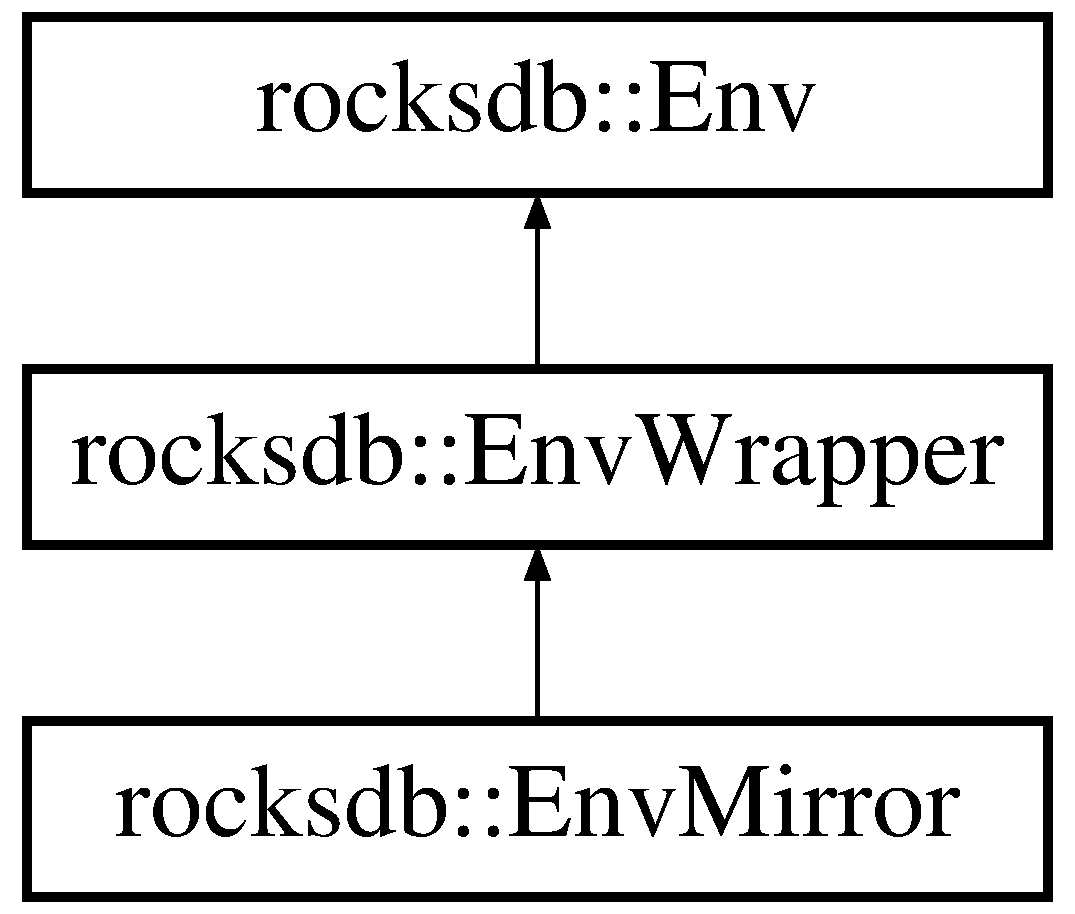
\includegraphics[height=3.000000cm]{classrocksdb_1_1EnvMirror}
\end{center}
\end{figure}
\subsection*{Classes}
\begin{DoxyCompactItemize}
\item 
class \hyperlink{classrocksdb_1_1EnvMirror_1_1FileLockMirror}{File\+Lock\+Mirror}
\end{DoxyCompactItemize}
\subsection*{Public Member Functions}
\begin{DoxyCompactItemize}
\item 
{\bfseries Env\+Mirror} (\hyperlink{classrocksdb_1_1Env}{Env} $\ast$a, \hyperlink{classrocksdb_1_1Env}{Env} $\ast$b)\hypertarget{classrocksdb_1_1EnvMirror_aa9d54e018f6c63551982ba4110010527}{}\label{classrocksdb_1_1EnvMirror_aa9d54e018f6c63551982ba4110010527}

\item 
\hyperlink{classrocksdb_1_1Status}{Status} {\bfseries New\+Sequential\+File} (const std\+::string \&f, unique\+\_\+ptr$<$ \hyperlink{classrocksdb_1_1SequentialFile}{Sequential\+File} $>$ $\ast$r, const \hyperlink{structrocksdb_1_1EnvOptions}{Env\+Options} \&options) override\hypertarget{classrocksdb_1_1EnvMirror_af42cb2435858ab1e73fd212a7b953c6a}{}\label{classrocksdb_1_1EnvMirror_af42cb2435858ab1e73fd212a7b953c6a}

\item 
\hyperlink{classrocksdb_1_1Status}{Status} {\bfseries New\+Random\+Access\+File} (const std\+::string \&f, unique\+\_\+ptr$<$ \hyperlink{classrocksdb_1_1RandomAccessFile}{Random\+Access\+File} $>$ $\ast$r, const \hyperlink{structrocksdb_1_1EnvOptions}{Env\+Options} \&options) override\hypertarget{classrocksdb_1_1EnvMirror_a4a192d3e03b23da2891392c43538f4fe}{}\label{classrocksdb_1_1EnvMirror_a4a192d3e03b23da2891392c43538f4fe}

\item 
\hyperlink{classrocksdb_1_1Status}{Status} {\bfseries New\+Writable\+File} (const std\+::string \&f, unique\+\_\+ptr$<$ \hyperlink{classrocksdb_1_1WritableFile}{Writable\+File} $>$ $\ast$r, const \hyperlink{structrocksdb_1_1EnvOptions}{Env\+Options} \&options) override\hypertarget{classrocksdb_1_1EnvMirror_ab0cd5ef3e36ddd53bf3a7f4d622fef1d}{}\label{classrocksdb_1_1EnvMirror_ab0cd5ef3e36ddd53bf3a7f4d622fef1d}

\item 
\hyperlink{classrocksdb_1_1Status}{Status} {\bfseries Reuse\+Writable\+File} (const std\+::string \&fname, const std\+::string \&old\+\_\+fname, unique\+\_\+ptr$<$ \hyperlink{classrocksdb_1_1WritableFile}{Writable\+File} $>$ $\ast$r, const \hyperlink{structrocksdb_1_1EnvOptions}{Env\+Options} \&options) override\hypertarget{classrocksdb_1_1EnvMirror_a19cf54de09f54692019c2bf7c720a705}{}\label{classrocksdb_1_1EnvMirror_a19cf54de09f54692019c2bf7c720a705}

\item 
virtual \hyperlink{classrocksdb_1_1Status}{Status} {\bfseries New\+Directory} (const std\+::string \&name, unique\+\_\+ptr$<$ \hyperlink{classrocksdb_1_1Directory}{Directory} $>$ $\ast$result) override\hypertarget{classrocksdb_1_1EnvMirror_ae325e2b590476a6bfbaaece47fbd007f}{}\label{classrocksdb_1_1EnvMirror_ae325e2b590476a6bfbaaece47fbd007f}

\item 
\hyperlink{classrocksdb_1_1Status}{Status} {\bfseries File\+Exists} (const std\+::string \&f) override\hypertarget{classrocksdb_1_1EnvMirror_aa678cb923cf3ce0ed7d63eed05e80a03}{}\label{classrocksdb_1_1EnvMirror_aa678cb923cf3ce0ed7d63eed05e80a03}

\item 
\hyperlink{classrocksdb_1_1Status}{Status} {\bfseries Get\+Children} (const std\+::string \&dir, std\+::vector$<$ std\+::string $>$ $\ast$r) override\hypertarget{classrocksdb_1_1EnvMirror_a1960df889f22e8a291685be525ce3a44}{}\label{classrocksdb_1_1EnvMirror_a1960df889f22e8a291685be525ce3a44}

\item 
\hyperlink{classrocksdb_1_1Status}{Status} {\bfseries Delete\+File} (const std\+::string \&f) override\hypertarget{classrocksdb_1_1EnvMirror_a24cc55f67dc4a8d709c7f8051a1798a2}{}\label{classrocksdb_1_1EnvMirror_a24cc55f67dc4a8d709c7f8051a1798a2}

\item 
\hyperlink{classrocksdb_1_1Status}{Status} {\bfseries Create\+Dir} (const std\+::string \&d) override\hypertarget{classrocksdb_1_1EnvMirror_aa22907e532ba18d3ab38fcadc40e52d2}{}\label{classrocksdb_1_1EnvMirror_aa22907e532ba18d3ab38fcadc40e52d2}

\item 
\hyperlink{classrocksdb_1_1Status}{Status} {\bfseries Create\+Dir\+If\+Missing} (const std\+::string \&d) override\hypertarget{classrocksdb_1_1EnvMirror_a47ffc0e4f721f3160abf26f2dd9d7017}{}\label{classrocksdb_1_1EnvMirror_a47ffc0e4f721f3160abf26f2dd9d7017}

\item 
\hyperlink{classrocksdb_1_1Status}{Status} {\bfseries Delete\+Dir} (const std\+::string \&d) override\hypertarget{classrocksdb_1_1EnvMirror_a40f31f2af0a4540241910e14734447cc}{}\label{classrocksdb_1_1EnvMirror_a40f31f2af0a4540241910e14734447cc}

\item 
\hyperlink{classrocksdb_1_1Status}{Status} {\bfseries Get\+File\+Size} (const std\+::string \&f, uint64\+\_\+t $\ast$s) override\hypertarget{classrocksdb_1_1EnvMirror_a25359fd3c7f4a5ca01c9690ca2e0e534}{}\label{classrocksdb_1_1EnvMirror_a25359fd3c7f4a5ca01c9690ca2e0e534}

\item 
\hyperlink{classrocksdb_1_1Status}{Status} {\bfseries Get\+File\+Modification\+Time} (const std\+::string \&fname, uint64\+\_\+t $\ast$file\+\_\+mtime) override\hypertarget{classrocksdb_1_1EnvMirror_a3ad82605cad55c6e4973a2fe5ca05d60}{}\label{classrocksdb_1_1EnvMirror_a3ad82605cad55c6e4973a2fe5ca05d60}

\item 
\hyperlink{classrocksdb_1_1Status}{Status} {\bfseries Rename\+File} (const std\+::string \&s, const std\+::string \&t) override\hypertarget{classrocksdb_1_1EnvMirror_ae59670ffb6ebe2e48e6dbac866d7fcb9}{}\label{classrocksdb_1_1EnvMirror_ae59670ffb6ebe2e48e6dbac866d7fcb9}

\item 
\hyperlink{classrocksdb_1_1Status}{Status} {\bfseries Link\+File} (const std\+::string \&s, const std\+::string \&t) override\hypertarget{classrocksdb_1_1EnvMirror_ab11999d851a8051d07e48d2a081b6196}{}\label{classrocksdb_1_1EnvMirror_ab11999d851a8051d07e48d2a081b6196}

\item 
\hyperlink{classrocksdb_1_1Status}{Status} {\bfseries Lock\+File} (const std\+::string \&f, \hyperlink{classrocksdb_1_1FileLock}{File\+Lock} $\ast$$\ast$l) override\hypertarget{classrocksdb_1_1EnvMirror_a8ff9c4ee9b25498704ff4685c073d14b}{}\label{classrocksdb_1_1EnvMirror_a8ff9c4ee9b25498704ff4685c073d14b}

\item 
\hyperlink{classrocksdb_1_1Status}{Status} {\bfseries Unlock\+File} (\hyperlink{classrocksdb_1_1FileLock}{File\+Lock} $\ast$l) override\hypertarget{classrocksdb_1_1EnvMirror_a9cf29cccefd183106a44d7810f44b83c}{}\label{classrocksdb_1_1EnvMirror_a9cf29cccefd183106a44d7810f44b83c}

\end{DoxyCompactItemize}
\subsection*{Additional Inherited Members}


The documentation for this class was generated from the following file\+:\begin{DoxyCompactItemize}
\item 
Appserver/src/external/rocksdb/utilities/env\+\_\+mirror.\+h\end{DoxyCompactItemize}

\hypertarget{structrocksdb_1_1EnvOptions}{}\section{rocksdb\+:\+:Env\+Options Struct Reference}
\label{structrocksdb_1_1EnvOptions}\index{rocksdb\+::\+Env\+Options@{rocksdb\+::\+Env\+Options}}
\subsection*{Public Member Functions}
\begin{DoxyCompactItemize}
\item 
{\bfseries Env\+Options} (const \hyperlink{structrocksdb_1_1DBOptions}{D\+B\+Options} \&options)\hypertarget{structrocksdb_1_1EnvOptions_a65453c22ddd76dc888089322c52581ce}{}\label{structrocksdb_1_1EnvOptions_a65453c22ddd76dc888089322c52581ce}

\end{DoxyCompactItemize}
\subsection*{Public Attributes}
\begin{DoxyCompactItemize}
\item 
bool {\bfseries use\+\_\+os\+\_\+buffer} = true\hypertarget{structrocksdb_1_1EnvOptions_a6e540588aa46118a79ae91ef620ee711}{}\label{structrocksdb_1_1EnvOptions_a6e540588aa46118a79ae91ef620ee711}

\item 
bool {\bfseries use\+\_\+mmap\+\_\+reads} = false\hypertarget{structrocksdb_1_1EnvOptions_a5c72ea7802f091ca6daa6c4722211265}{}\label{structrocksdb_1_1EnvOptions_a5c72ea7802f091ca6daa6c4722211265}

\item 
bool {\bfseries use\+\_\+mmap\+\_\+writes} = true\hypertarget{structrocksdb_1_1EnvOptions_ac07a355bb0a3d876f3c8c344ab5e8c41}{}\label{structrocksdb_1_1EnvOptions_ac07a355bb0a3d876f3c8c344ab5e8c41}

\item 
bool {\bfseries allow\+\_\+fallocate} = true\hypertarget{structrocksdb_1_1EnvOptions_a26296066fbb75476e6436b0b64fc5cfe}{}\label{structrocksdb_1_1EnvOptions_a26296066fbb75476e6436b0b64fc5cfe}

\item 
bool {\bfseries set\+\_\+fd\+\_\+cloexec} = true\hypertarget{structrocksdb_1_1EnvOptions_a2235129e25340b5970527ec2cce4aebd}{}\label{structrocksdb_1_1EnvOptions_a2235129e25340b5970527ec2cce4aebd}

\item 
uint64\+\_\+t {\bfseries bytes\+\_\+per\+\_\+sync} = 0\hypertarget{structrocksdb_1_1EnvOptions_a048b9773bcf18c325466e19d49f03fe4}{}\label{structrocksdb_1_1EnvOptions_a048b9773bcf18c325466e19d49f03fe4}

\item 
bool {\bfseries fallocate\+\_\+with\+\_\+keep\+\_\+size} = true\hypertarget{structrocksdb_1_1EnvOptions_a54b87413bd7df6d5fbdcdf04532f06a8}{}\label{structrocksdb_1_1EnvOptions_a54b87413bd7df6d5fbdcdf04532f06a8}

\item 
size\+\_\+t {\bfseries compaction\+\_\+readahead\+\_\+size}\hypertarget{structrocksdb_1_1EnvOptions_ac7275cb9afb4c346db0d9d160b42d004}{}\label{structrocksdb_1_1EnvOptions_ac7275cb9afb4c346db0d9d160b42d004}

\item 
size\+\_\+t {\bfseries random\+\_\+access\+\_\+max\+\_\+buffer\+\_\+size}\hypertarget{structrocksdb_1_1EnvOptions_a82bc43be4be53194894fa80da36cdb04}{}\label{structrocksdb_1_1EnvOptions_a82bc43be4be53194894fa80da36cdb04}

\item 
size\+\_\+t {\bfseries writable\+\_\+file\+\_\+max\+\_\+buffer\+\_\+size} = 1024 $\ast$ 1024\hypertarget{structrocksdb_1_1EnvOptions_adaec8cfd73c5ffa7677f803e381a93c1}{}\label{structrocksdb_1_1EnvOptions_adaec8cfd73c5ffa7677f803e381a93c1}

\item 
\hyperlink{classrocksdb_1_1RateLimiter}{Rate\+Limiter} $\ast$ {\bfseries rate\+\_\+limiter} = nullptr\hypertarget{structrocksdb_1_1EnvOptions_a7b400f9a1b10c03af13df7004597da3f}{}\label{structrocksdb_1_1EnvOptions_a7b400f9a1b10c03af13df7004597da3f}

\end{DoxyCompactItemize}


The documentation for this struct was generated from the following file\+:\begin{DoxyCompactItemize}
\item 
Appserver/src/external/rocksdb/env.\+h\end{DoxyCompactItemize}

\hypertarget{classrocksdb_1_1EnvWrapper}{}\section{rocksdb\+:\+:Env\+Wrapper Class Reference}
\label{classrocksdb_1_1EnvWrapper}\index{rocksdb\+::\+Env\+Wrapper@{rocksdb\+::\+Env\+Wrapper}}
Inheritance diagram for rocksdb\+:\+:Env\+Wrapper\+:\begin{figure}[H]
\begin{center}
\leavevmode
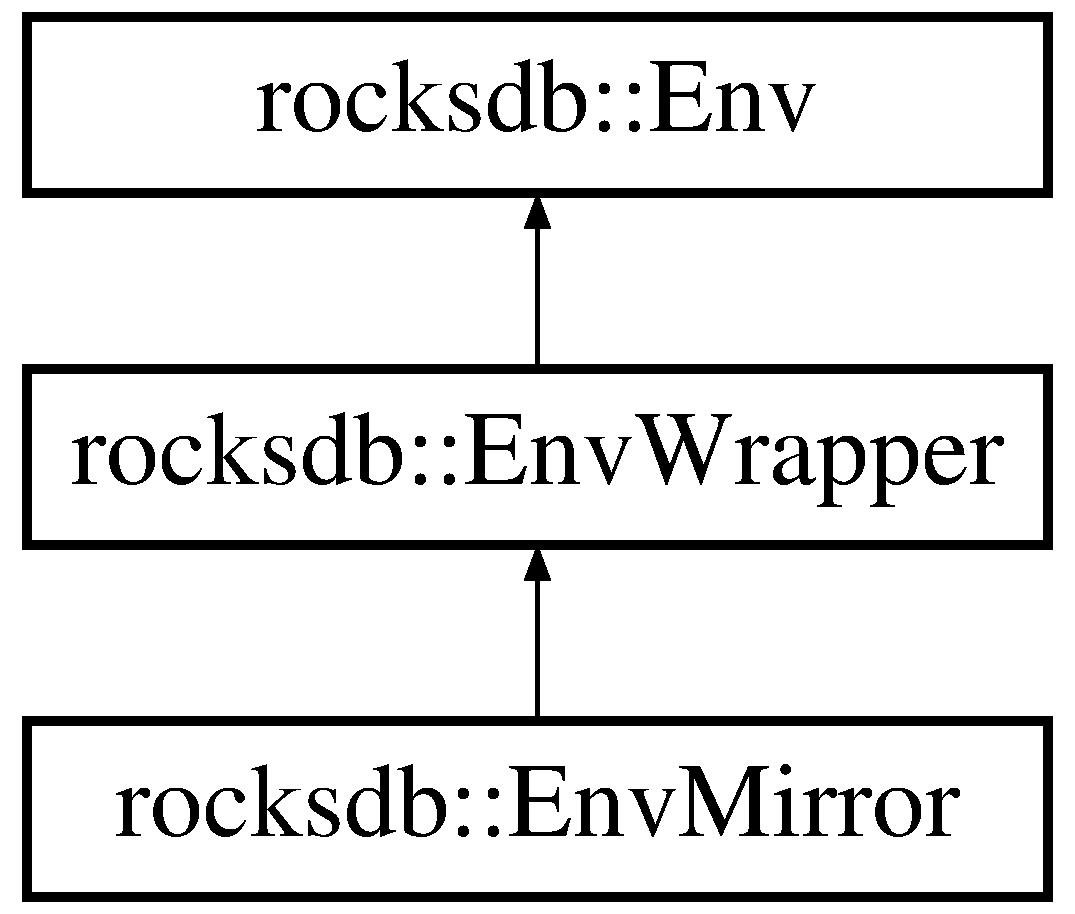
\includegraphics[height=3.000000cm]{classrocksdb_1_1EnvWrapper}
\end{center}
\end{figure}
\subsection*{Public Member Functions}
\begin{DoxyCompactItemize}
\item 
{\bfseries Env\+Wrapper} (\hyperlink{classrocksdb_1_1Env}{Env} $\ast$t)\hypertarget{classrocksdb_1_1EnvWrapper_ae37ae6de8a04752756d14b3d733e6e1e}{}\label{classrocksdb_1_1EnvWrapper_ae37ae6de8a04752756d14b3d733e6e1e}

\item 
\hyperlink{classrocksdb_1_1Env}{Env} $\ast$ {\bfseries target} () const\hypertarget{classrocksdb_1_1EnvWrapper_aefb72ca219c9b933fba9fc572cf84a3f}{}\label{classrocksdb_1_1EnvWrapper_aefb72ca219c9b933fba9fc572cf84a3f}

\item 
\hyperlink{classrocksdb_1_1Status}{Status} {\bfseries New\+Sequential\+File} (const std\+::string \&f, unique\+\_\+ptr$<$ \hyperlink{classrocksdb_1_1SequentialFile}{Sequential\+File} $>$ $\ast$r, const \hyperlink{structrocksdb_1_1EnvOptions}{Env\+Options} \&options) override\hypertarget{classrocksdb_1_1EnvWrapper_a16afc94e7dbb40a9f15d137d6675dc40}{}\label{classrocksdb_1_1EnvWrapper_a16afc94e7dbb40a9f15d137d6675dc40}

\item 
\hyperlink{classrocksdb_1_1Status}{Status} {\bfseries New\+Random\+Access\+File} (const std\+::string \&f, unique\+\_\+ptr$<$ \hyperlink{classrocksdb_1_1RandomAccessFile}{Random\+Access\+File} $>$ $\ast$r, const \hyperlink{structrocksdb_1_1EnvOptions}{Env\+Options} \&options) override\hypertarget{classrocksdb_1_1EnvWrapper_ac24f60f42e2af752e6cec45e958f4408}{}\label{classrocksdb_1_1EnvWrapper_ac24f60f42e2af752e6cec45e958f4408}

\item 
\hyperlink{classrocksdb_1_1Status}{Status} {\bfseries New\+Writable\+File} (const std\+::string \&f, unique\+\_\+ptr$<$ \hyperlink{classrocksdb_1_1WritableFile}{Writable\+File} $>$ $\ast$r, const \hyperlink{structrocksdb_1_1EnvOptions}{Env\+Options} \&options) override\hypertarget{classrocksdb_1_1EnvWrapper_a33a5adf52362df8b3502e4237071b108}{}\label{classrocksdb_1_1EnvWrapper_a33a5adf52362df8b3502e4237071b108}

\item 
\hyperlink{classrocksdb_1_1Status}{Status} {\bfseries Reuse\+Writable\+File} (const std\+::string \&fname, const std\+::string \&old\+\_\+fname, unique\+\_\+ptr$<$ \hyperlink{classrocksdb_1_1WritableFile}{Writable\+File} $>$ $\ast$r, const \hyperlink{structrocksdb_1_1EnvOptions}{Env\+Options} \&options) override\hypertarget{classrocksdb_1_1EnvWrapper_a734526bf94a33e59a3a4f9d973c72642}{}\label{classrocksdb_1_1EnvWrapper_a734526bf94a33e59a3a4f9d973c72642}

\item 
virtual \hyperlink{classrocksdb_1_1Status}{Status} {\bfseries New\+Directory} (const std\+::string \&name, unique\+\_\+ptr$<$ \hyperlink{classrocksdb_1_1Directory}{Directory} $>$ $\ast$result) override\hypertarget{classrocksdb_1_1EnvWrapper_af6a51b6a782c76e343d0762137bf462d}{}\label{classrocksdb_1_1EnvWrapper_af6a51b6a782c76e343d0762137bf462d}

\item 
\hyperlink{classrocksdb_1_1Status}{Status} {\bfseries File\+Exists} (const std\+::string \&f) override\hypertarget{classrocksdb_1_1EnvWrapper_a26e009afcc388524815ce1652afefb6c}{}\label{classrocksdb_1_1EnvWrapper_a26e009afcc388524815ce1652afefb6c}

\item 
\hyperlink{classrocksdb_1_1Status}{Status} {\bfseries Get\+Children} (const std\+::string \&dir, std\+::vector$<$ std\+::string $>$ $\ast$r) override\hypertarget{classrocksdb_1_1EnvWrapper_a88542d17182f47d14d5f717204c8b831}{}\label{classrocksdb_1_1EnvWrapper_a88542d17182f47d14d5f717204c8b831}

\item 
\hyperlink{classrocksdb_1_1Status}{Status} {\bfseries Get\+Children\+File\+Attributes} (const std\+::string \&dir, std\+::vector$<$ \hyperlink{structrocksdb_1_1Env_1_1FileAttributes}{File\+Attributes} $>$ $\ast$result) override\hypertarget{classrocksdb_1_1EnvWrapper_a5bbff8711a5422883d5a1bc73bbe1032}{}\label{classrocksdb_1_1EnvWrapper_a5bbff8711a5422883d5a1bc73bbe1032}

\item 
\hyperlink{classrocksdb_1_1Status}{Status} {\bfseries Delete\+File} (const std\+::string \&f) override\hypertarget{classrocksdb_1_1EnvWrapper_ad53db88a845b6691ec87ad45d3d27c9f}{}\label{classrocksdb_1_1EnvWrapper_ad53db88a845b6691ec87ad45d3d27c9f}

\item 
\hyperlink{classrocksdb_1_1Status}{Status} {\bfseries Create\+Dir} (const std\+::string \&d) override\hypertarget{classrocksdb_1_1EnvWrapper_a131daf98774112cf7b52a693519ed04a}{}\label{classrocksdb_1_1EnvWrapper_a131daf98774112cf7b52a693519ed04a}

\item 
\hyperlink{classrocksdb_1_1Status}{Status} {\bfseries Create\+Dir\+If\+Missing} (const std\+::string \&d) override\hypertarget{classrocksdb_1_1EnvWrapper_a780722e8cd623b67cb573e861b24476c}{}\label{classrocksdb_1_1EnvWrapper_a780722e8cd623b67cb573e861b24476c}

\item 
\hyperlink{classrocksdb_1_1Status}{Status} {\bfseries Delete\+Dir} (const std\+::string \&d) override\hypertarget{classrocksdb_1_1EnvWrapper_a671abf270a42b060531a33e57e6dda44}{}\label{classrocksdb_1_1EnvWrapper_a671abf270a42b060531a33e57e6dda44}

\item 
\hyperlink{classrocksdb_1_1Status}{Status} {\bfseries Get\+File\+Size} (const std\+::string \&f, uint64\+\_\+t $\ast$s) override\hypertarget{classrocksdb_1_1EnvWrapper_a2b10a24c1394464ce2a0d56d29a1a03c}{}\label{classrocksdb_1_1EnvWrapper_a2b10a24c1394464ce2a0d56d29a1a03c}

\item 
\hyperlink{classrocksdb_1_1Status}{Status} {\bfseries Get\+File\+Modification\+Time} (const std\+::string \&fname, uint64\+\_\+t $\ast$file\+\_\+mtime) override\hypertarget{classrocksdb_1_1EnvWrapper_a4e1147d6136e86eb0d082525839c1575}{}\label{classrocksdb_1_1EnvWrapper_a4e1147d6136e86eb0d082525839c1575}

\item 
\hyperlink{classrocksdb_1_1Status}{Status} {\bfseries Rename\+File} (const std\+::string \&s, const std\+::string \&t) override\hypertarget{classrocksdb_1_1EnvWrapper_a1d027dd3537ba577893df70232c35763}{}\label{classrocksdb_1_1EnvWrapper_a1d027dd3537ba577893df70232c35763}

\item 
\hyperlink{classrocksdb_1_1Status}{Status} {\bfseries Link\+File} (const std\+::string \&s, const std\+::string \&t) override\hypertarget{classrocksdb_1_1EnvWrapper_a35951d75c25be92c096d426e616dd670}{}\label{classrocksdb_1_1EnvWrapper_a35951d75c25be92c096d426e616dd670}

\item 
\hyperlink{classrocksdb_1_1Status}{Status} {\bfseries Lock\+File} (const std\+::string \&f, \hyperlink{classrocksdb_1_1FileLock}{File\+Lock} $\ast$$\ast$l) override\hypertarget{classrocksdb_1_1EnvWrapper_a3864487300905a1dc31172530b0d68a9}{}\label{classrocksdb_1_1EnvWrapper_a3864487300905a1dc31172530b0d68a9}

\item 
\hyperlink{classrocksdb_1_1Status}{Status} {\bfseries Unlock\+File} (\hyperlink{classrocksdb_1_1FileLock}{File\+Lock} $\ast$l) override\hypertarget{classrocksdb_1_1EnvWrapper_af4ed5505a79bf2469aee41b071e65772}{}\label{classrocksdb_1_1EnvWrapper_af4ed5505a79bf2469aee41b071e65772}

\item 
void {\bfseries Schedule} (void($\ast$f)(void $\ast$arg), void $\ast$a, Priority pri, void $\ast$tag=nullptr, void($\ast$u)(void $\ast$arg)=0) override\hypertarget{classrocksdb_1_1EnvWrapper_a4dcc1d168f1a6313df4c0272259d7dce}{}\label{classrocksdb_1_1EnvWrapper_a4dcc1d168f1a6313df4c0272259d7dce}

\item 
int {\bfseries Un\+Schedule} (void $\ast$tag, Priority pri) override\hypertarget{classrocksdb_1_1EnvWrapper_ae8d7a993c3d59951738942283241b76f}{}\label{classrocksdb_1_1EnvWrapper_ae8d7a993c3d59951738942283241b76f}

\item 
void {\bfseries Start\+Thread} (void($\ast$f)(void $\ast$), void $\ast$a) override\hypertarget{classrocksdb_1_1EnvWrapper_aca39b00f12a10b25a29cf80bc877bcd7}{}\label{classrocksdb_1_1EnvWrapper_aca39b00f12a10b25a29cf80bc877bcd7}

\item 
void {\bfseries Wait\+For\+Join} () override\hypertarget{classrocksdb_1_1EnvWrapper_aeb73bcae1e862c28c1facf89c6bdc004}{}\label{classrocksdb_1_1EnvWrapper_aeb73bcae1e862c28c1facf89c6bdc004}

\item 
virtual unsigned int {\bfseries Get\+Thread\+Pool\+Queue\+Len} (Priority pri=L\+OW) const override\hypertarget{classrocksdb_1_1EnvWrapper_ad793f330cd75416daac2942f27dbbaa4}{}\label{classrocksdb_1_1EnvWrapper_ad793f330cd75416daac2942f27dbbaa4}

\item 
virtual \hyperlink{classrocksdb_1_1Status}{Status} {\bfseries Get\+Test\+Directory} (std\+::string $\ast$path) override\hypertarget{classrocksdb_1_1EnvWrapper_a317ac22205c71a9149ac281a2099eea8}{}\label{classrocksdb_1_1EnvWrapper_a317ac22205c71a9149ac281a2099eea8}

\item 
virtual \hyperlink{classrocksdb_1_1Status}{Status} {\bfseries New\+Logger} (const std\+::string \&fname, shared\+\_\+ptr$<$ \hyperlink{classrocksdb_1_1Logger}{Logger} $>$ $\ast$result) override\hypertarget{classrocksdb_1_1EnvWrapper_a2980b8dc1cd6861ab3ed58e57b6b7de1}{}\label{classrocksdb_1_1EnvWrapper_a2980b8dc1cd6861ab3ed58e57b6b7de1}

\item 
uint64\+\_\+t {\bfseries Now\+Micros} () override\hypertarget{classrocksdb_1_1EnvWrapper_aa37120924c92abc8dcc877b030e2e85e}{}\label{classrocksdb_1_1EnvWrapper_aa37120924c92abc8dcc877b030e2e85e}

\item 
void {\bfseries Sleep\+For\+Microseconds} (int micros) override\hypertarget{classrocksdb_1_1EnvWrapper_aead93103f08a912aa82ae4d67a4d58eb}{}\label{classrocksdb_1_1EnvWrapper_aead93103f08a912aa82ae4d67a4d58eb}

\item 
\hyperlink{classrocksdb_1_1Status}{Status} {\bfseries Get\+Host\+Name} (char $\ast$name, uint64\+\_\+t len) override\hypertarget{classrocksdb_1_1EnvWrapper_a0351d4fc6a66eb8131ccd8c1874dbb8f}{}\label{classrocksdb_1_1EnvWrapper_a0351d4fc6a66eb8131ccd8c1874dbb8f}

\item 
\hyperlink{classrocksdb_1_1Status}{Status} {\bfseries Get\+Current\+Time} (int64\+\_\+t $\ast$unix\+\_\+time) override\hypertarget{classrocksdb_1_1EnvWrapper_a9e4488f871063d0fd72f0fd2919610aa}{}\label{classrocksdb_1_1EnvWrapper_a9e4488f871063d0fd72f0fd2919610aa}

\item 
\hyperlink{classrocksdb_1_1Status}{Status} {\bfseries Get\+Absolute\+Path} (const std\+::string \&db\+\_\+path, std\+::string $\ast$output\+\_\+path) override\hypertarget{classrocksdb_1_1EnvWrapper_a0e10fc987cd3e93ed4f2150e2af350e2}{}\label{classrocksdb_1_1EnvWrapper_a0e10fc987cd3e93ed4f2150e2af350e2}

\item 
void {\bfseries Set\+Background\+Threads} (int num, Priority pri) override\hypertarget{classrocksdb_1_1EnvWrapper_a8fcba7e9f6a8b1fbfd59dbe2aeda5dea}{}\label{classrocksdb_1_1EnvWrapper_a8fcba7e9f6a8b1fbfd59dbe2aeda5dea}

\item 
void {\bfseries Inc\+Background\+Threads\+If\+Needed} (int num, Priority pri) override\hypertarget{classrocksdb_1_1EnvWrapper_a176f3b118d6bbf42d94169c4c2d66814}{}\label{classrocksdb_1_1EnvWrapper_a176f3b118d6bbf42d94169c4c2d66814}

\item 
void {\bfseries Lower\+Thread\+Pool\+I\+O\+Priority} (Priority pool=L\+OW) override\hypertarget{classrocksdb_1_1EnvWrapper_afa78d2ed1ba4c848345cb06175cefa72}{}\label{classrocksdb_1_1EnvWrapper_afa78d2ed1ba4c848345cb06175cefa72}

\item 
std\+::string {\bfseries Time\+To\+String} (uint64\+\_\+t time) override\hypertarget{classrocksdb_1_1EnvWrapper_ab85d8bb25a5b465f6dac690bbb2f3f1a}{}\label{classrocksdb_1_1EnvWrapper_ab85d8bb25a5b465f6dac690bbb2f3f1a}

\item 
\hyperlink{classrocksdb_1_1Status}{Status} {\bfseries Get\+Thread\+List} (std\+::vector$<$ \hyperlink{structrocksdb_1_1ThreadStatus}{Thread\+Status} $>$ $\ast$thread\+\_\+list) override\hypertarget{classrocksdb_1_1EnvWrapper_a8b98931ac26c2a4726e2702d5ea2ecb7}{}\label{classrocksdb_1_1EnvWrapper_a8b98931ac26c2a4726e2702d5ea2ecb7}

\item 
Thread\+Status\+Updater $\ast$ {\bfseries Get\+Thread\+Status\+Updater} () const override\hypertarget{classrocksdb_1_1EnvWrapper_a0a2049d06aad5884a104c216959a9c50}{}\label{classrocksdb_1_1EnvWrapper_a0a2049d06aad5884a104c216959a9c50}

\item 
uint64\+\_\+t {\bfseries Get\+Thread\+ID} () const override\hypertarget{classrocksdb_1_1EnvWrapper_a96c45c0226e3bbb4714e7c695be97c6f}{}\label{classrocksdb_1_1EnvWrapper_a96c45c0226e3bbb4714e7c695be97c6f}

\end{DoxyCompactItemize}
\subsection*{Additional Inherited Members}


The documentation for this class was generated from the following file\+:\begin{DoxyCompactItemize}
\item 
Appserver/src/external/rocksdb/env.\+h\end{DoxyCompactItemize}

\hypertarget{structEstadisticas}{}\section{Estadisticas Struct Reference}
\label{structEstadisticas}\index{Estadisticas@{Estadisticas}}
\subsection*{Public Attributes}
\begin{DoxyCompactItemize}
\item 
string {\bfseries usuario}\hypertarget{structEstadisticas_a34fd4a5ca7aef637cb68968fb21158e1}{}\label{structEstadisticas_a34fd4a5ca7aef637cb68968fb21158e1}

\item 
int {\bfseries cantidad\+De\+Candidatos\+Pedidos}\hypertarget{structEstadisticas_aeced7a8c6a195eb0f67860449af9970e}{}\label{structEstadisticas_aeced7a8c6a195eb0f67860449af9970e}

\item 
int {\bfseries cantidad\+De\+Votos\+Positivos}\hypertarget{structEstadisticas_a7d84124f5d54b25bc964ecd241ea6fc3}{}\label{structEstadisticas_a7d84124f5d54b25bc964ecd241ea6fc3}

\end{DoxyCompactItemize}


The documentation for this struct was generated from the following file\+:\begin{DoxyCompactItemize}
\item 
Appserver/src/servicios/Estadisticas\+Candidatos.\+h\end{DoxyCompactItemize}

\hypertarget{classEstadisticasCandidatos}{}\section{Estadisticas\+Candidatos Class Reference}
\label{classEstadisticasCandidatos}\index{Estadisticas\+Candidatos@{Estadisticas\+Candidatos}}
\subsection*{Public Member Functions}
\begin{DoxyCompactItemize}
\item 
void {\bfseries inicializar\+Usuario} (string usuario)\hypertarget{classEstadisticasCandidatos_af27e013c08328f2135fa062d80157e78}{}\label{classEstadisticasCandidatos_af27e013c08328f2135fa062d80157e78}

\item 
void {\bfseries contabilizar\+Candidato\+Para} (string usuario)\hypertarget{classEstadisticasCandidatos_a024e1d4eefb1b58ec5dda6a7b899bf6e}{}\label{classEstadisticasCandidatos_a024e1d4eefb1b58ec5dda6a7b899bf6e}

\item 
bool {\bfseries usuario\+Supero\+Limite\+De\+Candidatos} (string usuario)\hypertarget{classEstadisticasCandidatos_a5d1beb17279826cbd8f95fc4c41b404d}{}\label{classEstadisticasCandidatos_a5d1beb17279826cbd8f95fc4c41b404d}

\item 
void {\bfseries contabilizar\+Voto\+Para} (string usuario)\hypertarget{classEstadisticasCandidatos_a8cda91671f8cc425ad31a13a411162ff}{}\label{classEstadisticasCandidatos_a8cda91671f8cc425ad31a13a411162ff}

\item 
bool {\bfseries usuario\+Es\+Popular} (string usuario)\hypertarget{classEstadisticasCandidatos_a39939198d502a29bc5656e5861d403cf}{}\label{classEstadisticasCandidatos_a39939198d502a29bc5656e5861d403cf}

\end{DoxyCompactItemize}
\subsection*{Static Public Attributes}
\begin{DoxyCompactItemize}
\item 
static const int {\bfseries limite\+Candidatos} = 3\hypertarget{classEstadisticasCandidatos_ad44929762ff0508850e8c2046fb3d6d5}{}\label{classEstadisticasCandidatos_ad44929762ff0508850e8c2046fb3d6d5}

\item 
static const double {\bfseries porcentaje\+Usuarios\+Populares} = 0.\+01\hypertarget{classEstadisticasCandidatos_a6419176ded35f03972e7896c842e10f0}{}\label{classEstadisticasCandidatos_a6419176ded35f03972e7896c842e10f0}

\end{DoxyCompactItemize}


The documentation for this class was generated from the following files\+:\begin{DoxyCompactItemize}
\item 
Appserver/src/servicios/Estadisticas\+Candidatos.\+h\item 
Appserver/src/servicios/Estadisticas\+Candidatos.\+cpp\end{DoxyCompactItemize}

\hypertarget{classrocksdb_1_1EventListener}{}\section{rocksdb\+:\+:Event\+Listener Class Reference}
\label{classrocksdb_1_1EventListener}\index{rocksdb\+::\+Event\+Listener@{rocksdb\+::\+Event\+Listener}}
\subsection*{Public Member Functions}
\begin{DoxyCompactItemize}
\item 
virtual void {\bfseries On\+Flush\+Completed} (\hyperlink{classrocksdb_1_1DB}{DB} $\ast$, const \hyperlink{structrocksdb_1_1FlushJobInfo}{Flush\+Job\+Info} \&)\hypertarget{classrocksdb_1_1EventListener_a8fcc86998faf5d9f6f078b92ff3f6e7d}{}\label{classrocksdb_1_1EventListener_a8fcc86998faf5d9f6f078b92ff3f6e7d}

\item 
virtual void {\bfseries On\+Table\+File\+Deleted} (const \hyperlink{structrocksdb_1_1TableFileDeletionInfo}{Table\+File\+Deletion\+Info} \&)\hypertarget{classrocksdb_1_1EventListener_a0c108c91575be66bd451d00046f058f6}{}\label{classrocksdb_1_1EventListener_a0c108c91575be66bd451d00046f058f6}

\item 
virtual void {\bfseries On\+Compaction\+Completed} (\hyperlink{classrocksdb_1_1DB}{DB} $\ast$, const \hyperlink{structrocksdb_1_1CompactionJobInfo}{Compaction\+Job\+Info} \&)\hypertarget{classrocksdb_1_1EventListener_a9d73a0ed8e6558c4b20d34935c26b68e}{}\label{classrocksdb_1_1EventListener_a9d73a0ed8e6558c4b20d34935c26b68e}

\item 
virtual void {\bfseries On\+Table\+File\+Created} (const \hyperlink{structrocksdb_1_1TableFileCreationInfo}{Table\+File\+Creation\+Info} \&)\hypertarget{classrocksdb_1_1EventListener_a3d03220a975dd2bf67fbdd22c52cff3f}{}\label{classrocksdb_1_1EventListener_a3d03220a975dd2bf67fbdd22c52cff3f}

\end{DoxyCompactItemize}


The documentation for this class was generated from the following file\+:\begin{DoxyCompactItemize}
\item 
Appserver/src/external/rocksdb/listener.\+h\end{DoxyCompactItemize}

\hypertarget{classJson_1_1Exception}{}\section{Json\+:\+:Exception Class Reference}
\label{classJson_1_1Exception}\index{Json\+::\+Exception@{Json\+::\+Exception}}


{\ttfamily \#include $<$json.\+h$>$}

Inheritance diagram for Json\+:\+:Exception\+:\begin{figure}[H]
\begin{center}
\leavevmode
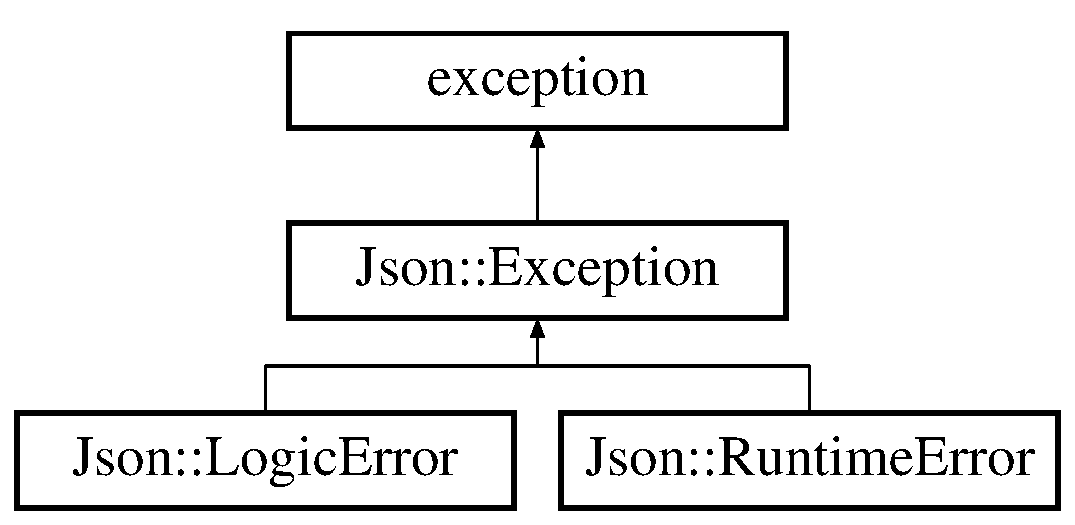
\includegraphics[height=3.000000cm]{classJson_1_1Exception}
\end{center}
\end{figure}
\subsection*{Public Member Functions}
\begin{DoxyCompactItemize}
\item 
{\bfseries Exception} (J\+S\+O\+N\+C\+P\+P\+\_\+\+S\+T\+R\+I\+NG const \&msg)\hypertarget{classJson_1_1Exception_ae764aa42e0755bd4ce9d303e2733fa8f}{}\label{classJson_1_1Exception_ae764aa42e0755bd4ce9d303e2733fa8f}

\item 
char const  $\ast$ {\bfseries what} () const J\+S\+O\+N\+C\+P\+P\+\_\+\+O\+V\+E\+R\+R\+I\+DE  throw ()\hypertarget{classJson_1_1Exception_ae84647676cb4eeca23de8b5723f10b11}{}\label{classJson_1_1Exception_ae84647676cb4eeca23de8b5723f10b11}

\end{DoxyCompactItemize}
\subsection*{Protected Attributes}
\begin{DoxyCompactItemize}
\item 
J\+S\+O\+N\+C\+P\+P\+\_\+\+S\+T\+R\+I\+NG {\bfseries msg\+\_\+}\hypertarget{classJson_1_1Exception_aae3cbb8b45bf21480f64502a8329659f}{}\label{classJson_1_1Exception_aae3cbb8b45bf21480f64502a8329659f}

\end{DoxyCompactItemize}


\subsection{Detailed Description}
Base class for all exceptions we throw.

We use nothing but these internally. Of course, S\+TL can throw others. 

The documentation for this class was generated from the following files\+:\begin{DoxyCompactItemize}
\item 
Appserver/src/external/json/json.\+h\item 
Appserver/src/external/json/jsoncpp.\+cpp\end{DoxyCompactItemize}

\hypertarget{structrocksdb_1_1ExternalSstFileInfo}{}\section{rocksdb\+:\+:External\+Sst\+File\+Info Struct Reference}
\label{structrocksdb_1_1ExternalSstFileInfo}\index{rocksdb\+::\+External\+Sst\+File\+Info@{rocksdb\+::\+External\+Sst\+File\+Info}}
\subsection*{Public Member Functions}
\begin{DoxyCompactItemize}
\item 
{\bfseries External\+Sst\+File\+Info} (const std\+::string \&\+\_\+file\+\_\+path, const std\+::string \&\+\_\+smallest\+\_\+key, const std\+::string \&\+\_\+largest\+\_\+key, Sequence\+Number \+\_\+sequence\+\_\+number, uint64\+\_\+t \+\_\+file\+\_\+size, int32\+\_\+t \+\_\+num\+\_\+entries, int32\+\_\+t \+\_\+version)\hypertarget{structrocksdb_1_1ExternalSstFileInfo_a7e63e1daef5c43b78284a1d0c2a72c5a}{}\label{structrocksdb_1_1ExternalSstFileInfo_a7e63e1daef5c43b78284a1d0c2a72c5a}

\end{DoxyCompactItemize}
\subsection*{Public Attributes}
\begin{DoxyCompactItemize}
\item 
std\+::string {\bfseries file\+\_\+path}\hypertarget{structrocksdb_1_1ExternalSstFileInfo_ab0ce3ae57eb85a27a8cad451aa4d0500}{}\label{structrocksdb_1_1ExternalSstFileInfo_ab0ce3ae57eb85a27a8cad451aa4d0500}

\item 
std\+::string {\bfseries smallest\+\_\+key}\hypertarget{structrocksdb_1_1ExternalSstFileInfo_ad3881c42fccc3d1607632759dd7b47ff}{}\label{structrocksdb_1_1ExternalSstFileInfo_ad3881c42fccc3d1607632759dd7b47ff}

\item 
std\+::string {\bfseries largest\+\_\+key}\hypertarget{structrocksdb_1_1ExternalSstFileInfo_a7be737ed8cba93c52a3df94f96b1e9aa}{}\label{structrocksdb_1_1ExternalSstFileInfo_a7be737ed8cba93c52a3df94f96b1e9aa}

\item 
Sequence\+Number {\bfseries sequence\+\_\+number}\hypertarget{structrocksdb_1_1ExternalSstFileInfo_a3e89f2383da012bbabae9df783e41931}{}\label{structrocksdb_1_1ExternalSstFileInfo_a3e89f2383da012bbabae9df783e41931}

\item 
uint64\+\_\+t {\bfseries file\+\_\+size}\hypertarget{structrocksdb_1_1ExternalSstFileInfo_a943f0e9b49a1ceb6d0b224ad22f40f70}{}\label{structrocksdb_1_1ExternalSstFileInfo_a943f0e9b49a1ceb6d0b224ad22f40f70}

\item 
uint64\+\_\+t {\bfseries num\+\_\+entries}\hypertarget{structrocksdb_1_1ExternalSstFileInfo_a0ff1cb083e40c776e4dcf3ecabbc841c}{}\label{structrocksdb_1_1ExternalSstFileInfo_a0ff1cb083e40c776e4dcf3ecabbc841c}

\item 
int32\+\_\+t {\bfseries version}\hypertarget{structrocksdb_1_1ExternalSstFileInfo_a87e05c58b50379028da9402ca838e6a8}{}\label{structrocksdb_1_1ExternalSstFileInfo_a87e05c58b50379028da9402ca838e6a8}

\end{DoxyCompactItemize}


The documentation for this struct was generated from the following file\+:\begin{DoxyCompactItemize}
\item 
Appserver/src/external/rocksdb/sst\+\_\+file\+\_\+writer.\+h\end{DoxyCompactItemize}

\hypertarget{structrocksdb_1_1ExternalSstFilePropertyNames}{}\section{rocksdb\+:\+:External\+Sst\+File\+Property\+Names Struct Reference}
\label{structrocksdb_1_1ExternalSstFilePropertyNames}\index{rocksdb\+::\+External\+Sst\+File\+Property\+Names@{rocksdb\+::\+External\+Sst\+File\+Property\+Names}}
\subsection*{Static Public Attributes}
\begin{DoxyCompactItemize}
\item 
static const std\+::string {\bfseries k\+Version}\hypertarget{structrocksdb_1_1ExternalSstFilePropertyNames_accb9b0ca917e37e71c524a171be69e01}{}\label{structrocksdb_1_1ExternalSstFilePropertyNames_accb9b0ca917e37e71c524a171be69e01}

\end{DoxyCompactItemize}


The documentation for this struct was generated from the following file\+:\begin{DoxyCompactItemize}
\item 
Appserver/src/external/rocksdb/sst\+\_\+file\+\_\+writer.\+h\end{DoxyCompactItemize}

\hypertarget{classJson_1_1CharReader_1_1Factory}{}\section{Json\+:\+:Char\+Reader\+:\+:Factory Class Reference}
\label{classJson_1_1CharReader_1_1Factory}\index{Json\+::\+Char\+Reader\+::\+Factory@{Json\+::\+Char\+Reader\+::\+Factory}}
Inheritance diagram for Json\+:\+:Char\+Reader\+:\+:Factory\+:\begin{figure}[H]
\begin{center}
\leavevmode
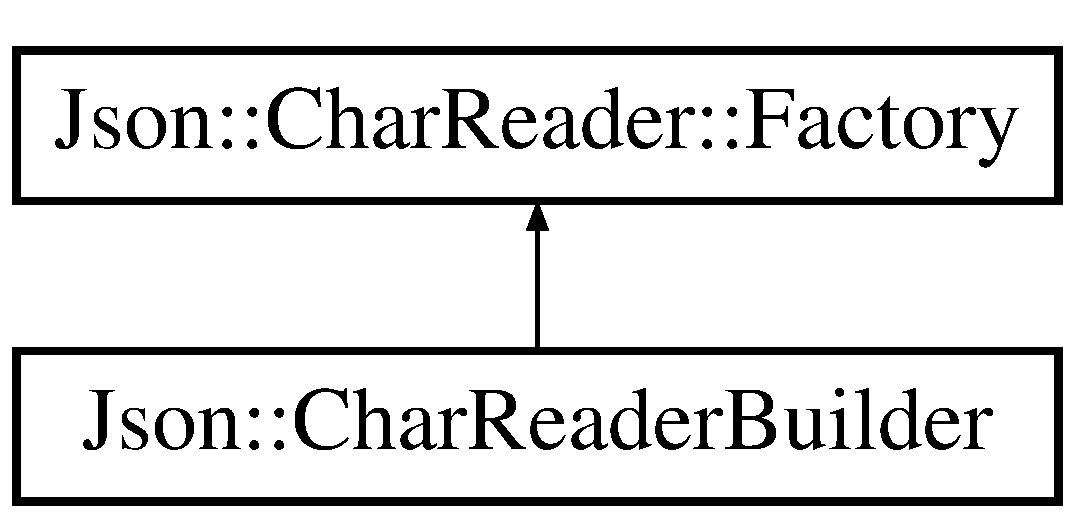
\includegraphics[height=2.000000cm]{classJson_1_1CharReader_1_1Factory}
\end{center}
\end{figure}
\subsection*{Public Member Functions}
\begin{DoxyCompactItemize}
\item 
virtual \hyperlink{classJson_1_1CharReader}{Char\+Reader} $\ast$ \hyperlink{classJson_1_1CharReader_1_1Factory_a4c5862a1ffd432372dbe65cf59de98c4}{new\+Char\+Reader} () const =0
\begin{DoxyCompactList}\small\item\em Allocate a \hyperlink{classJson_1_1CharReader}{Char\+Reader} via operator new(). \end{DoxyCompactList}\end{DoxyCompactItemize}


\subsection{Member Function Documentation}
\index{Json\+::\+Char\+Reader\+::\+Factory@{Json\+::\+Char\+Reader\+::\+Factory}!new\+Char\+Reader@{new\+Char\+Reader}}
\index{new\+Char\+Reader@{new\+Char\+Reader}!Json\+::\+Char\+Reader\+::\+Factory@{Json\+::\+Char\+Reader\+::\+Factory}}
\subsubsection[{\texorpdfstring{new\+Char\+Reader() const =0}{newCharReader() const =0}}]{\setlength{\rightskip}{0pt plus 5cm}virtual {\bf Char\+Reader}$\ast$ Json\+::\+Char\+Reader\+::\+Factory\+::new\+Char\+Reader (
\begin{DoxyParamCaption}
{}
\end{DoxyParamCaption}
) const\hspace{0.3cm}{\ttfamily [pure virtual]}}\hypertarget{classJson_1_1CharReader_1_1Factory_a4c5862a1ffd432372dbe65cf59de98c4}{}\label{classJson_1_1CharReader_1_1Factory_a4c5862a1ffd432372dbe65cf59de98c4}


Allocate a \hyperlink{classJson_1_1CharReader}{Char\+Reader} via operator new(). 


\begin{DoxyExceptions}{Exceptions}
{\em std\+::exception} & if something goes wrong (e.\+g. invalid settings) \\
\hline
\end{DoxyExceptions}


Implemented in \hyperlink{classJson_1_1CharReaderBuilder_a3a262fcc76c1eb8eebfd4718fb4e9722}{Json\+::\+Char\+Reader\+Builder}.



The documentation for this class was generated from the following file\+:\begin{DoxyCompactItemize}
\item 
Appserver/src/external/json/json.\+h\end{DoxyCompactItemize}

\hypertarget{classJson_1_1StreamWriter_1_1Factory}{}\section{Json\+:\+:Stream\+Writer\+:\+:Factory Class Reference}
\label{classJson_1_1StreamWriter_1_1Factory}\index{Json\+::\+Stream\+Writer\+::\+Factory@{Json\+::\+Stream\+Writer\+::\+Factory}}


A simple abstract factory.  




{\ttfamily \#include $<$json.\+h$>$}

Inheritance diagram for Json\+:\+:Stream\+Writer\+:\+:Factory\+:\begin{figure}[H]
\begin{center}
\leavevmode
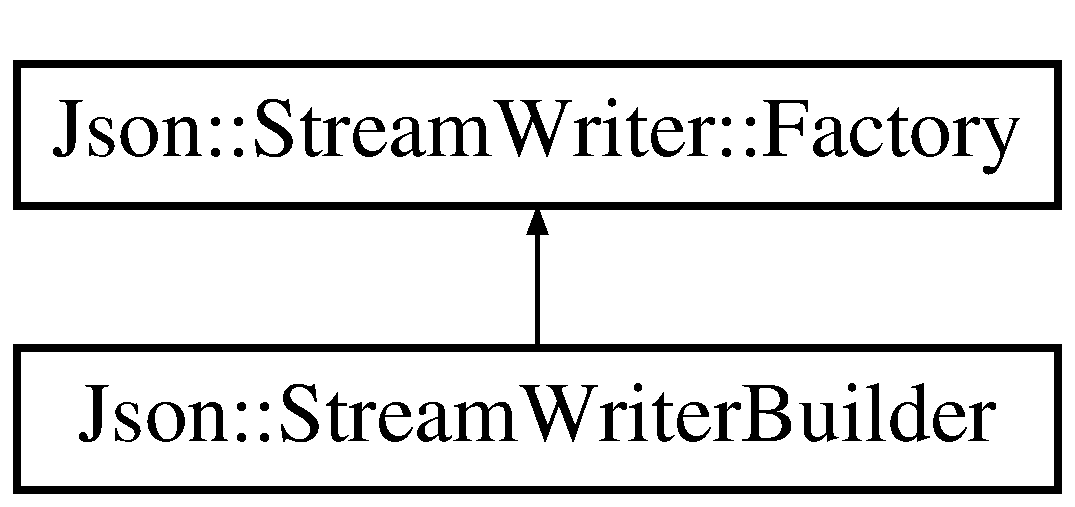
\includegraphics[height=2.000000cm]{classJson_1_1StreamWriter_1_1Factory}
\end{center}
\end{figure}
\subsection*{Public Member Functions}
\begin{DoxyCompactItemize}
\item 
virtual \hyperlink{classJson_1_1StreamWriter}{Stream\+Writer} $\ast$ \hyperlink{classJson_1_1StreamWriter_1_1Factory_a9d30ec53e8288cd53befccf1009c5f31}{new\+Stream\+Writer} () const =0
\begin{DoxyCompactList}\small\item\em Allocate a \hyperlink{classJson_1_1CharReader}{Char\+Reader} via operator new(). \end{DoxyCompactList}\end{DoxyCompactItemize}


\subsection{Detailed Description}
A simple abstract factory. 

\subsection{Member Function Documentation}
\index{Json\+::\+Stream\+Writer\+::\+Factory@{Json\+::\+Stream\+Writer\+::\+Factory}!new\+Stream\+Writer@{new\+Stream\+Writer}}
\index{new\+Stream\+Writer@{new\+Stream\+Writer}!Json\+::\+Stream\+Writer\+::\+Factory@{Json\+::\+Stream\+Writer\+::\+Factory}}
\subsubsection[{\texorpdfstring{new\+Stream\+Writer() const =0}{newStreamWriter() const =0}}]{\setlength{\rightskip}{0pt plus 5cm}virtual {\bf Stream\+Writer}$\ast$ Json\+::\+Stream\+Writer\+::\+Factory\+::new\+Stream\+Writer (
\begin{DoxyParamCaption}
{}
\end{DoxyParamCaption}
) const\hspace{0.3cm}{\ttfamily [pure virtual]}}\hypertarget{classJson_1_1StreamWriter_1_1Factory_a9d30ec53e8288cd53befccf1009c5f31}{}\label{classJson_1_1StreamWriter_1_1Factory_a9d30ec53e8288cd53befccf1009c5f31}


Allocate a \hyperlink{classJson_1_1CharReader}{Char\+Reader} via operator new(). 


\begin{DoxyExceptions}{Exceptions}
{\em std\+::exception} & if something goes wrong (e.\+g. invalid settings) \\
\hline
\end{DoxyExceptions}


Implemented in \hyperlink{classJson_1_1StreamWriterBuilder_ab9ee278609f88ae04a7c1a84e1f559e6}{Json\+::\+Stream\+Writer\+Builder}.



The documentation for this class was generated from the following files\+:\begin{DoxyCompactItemize}
\item 
Appserver/src/external/json/json.\+h\item 
Appserver/src/external/json/jsoncpp.\+cpp\end{DoxyCompactItemize}

\hypertarget{classFactoryServicios}{}\section{Factory\+Servicios Class Reference}
\label{classFactoryServicios}\index{Factory\+Servicios@{Factory\+Servicios}}
\subsection*{Public Member Functions}
\begin{DoxyCompactItemize}
\item 
{\bfseries Factory\+Servicios} (\hyperlink{classManejadorDeConexiones}{Manejador\+De\+Conexiones} $\ast$conexiones)\hypertarget{classFactoryServicios_abb22835c51090de62025e2469704373c}{}\label{classFactoryServicios_abb22835c51090de62025e2469704373c}

\item 
\hyperlink{classServicio}{Servicio} $\ast$ {\bfseries fabricar\+Servicio} (\hyperlink{classMensajeHTTPRequest}{Mensaje\+H\+T\+T\+P\+Request})\hypertarget{classFactoryServicios_ab2cb5f05cf87a872852e25d230b6d735}{}\label{classFactoryServicios_ab2cb5f05cf87a872852e25d230b6d735}

\item 
void {\bfseries cambiar\+Shared} (string direccion)\hypertarget{classFactoryServicios_ae3035afd7f39d3fbaa9d0da11c1550da}{}\label{classFactoryServicios_ae3035afd7f39d3fbaa9d0da11c1550da}

\end{DoxyCompactItemize}


The documentation for this class was generated from the following files\+:\begin{DoxyCompactItemize}
\item 
Appserver/src/servicios/Factory\+Servicios.\+h\item 
Appserver/src/servicios/Factory\+Servicios.\+cpp\end{DoxyCompactItemize}

\hypertarget{classJson_1_1FastWriter}{}\section{Json\+:\+:Fast\+Writer Class Reference}
\label{classJson_1_1FastWriter}\index{Json\+::\+Fast\+Writer@{Json\+::\+Fast\+Writer}}


Outputs a \hyperlink{classJson_1_1Value}{Value} in \href{http://www.json.org}{\tt J\+S\+ON} format without formatting (not human friendly).  




{\ttfamily \#include $<$json.\+h$>$}

Inheritance diagram for Json\+:\+:Fast\+Writer\+:\begin{figure}[H]
\begin{center}
\leavevmode
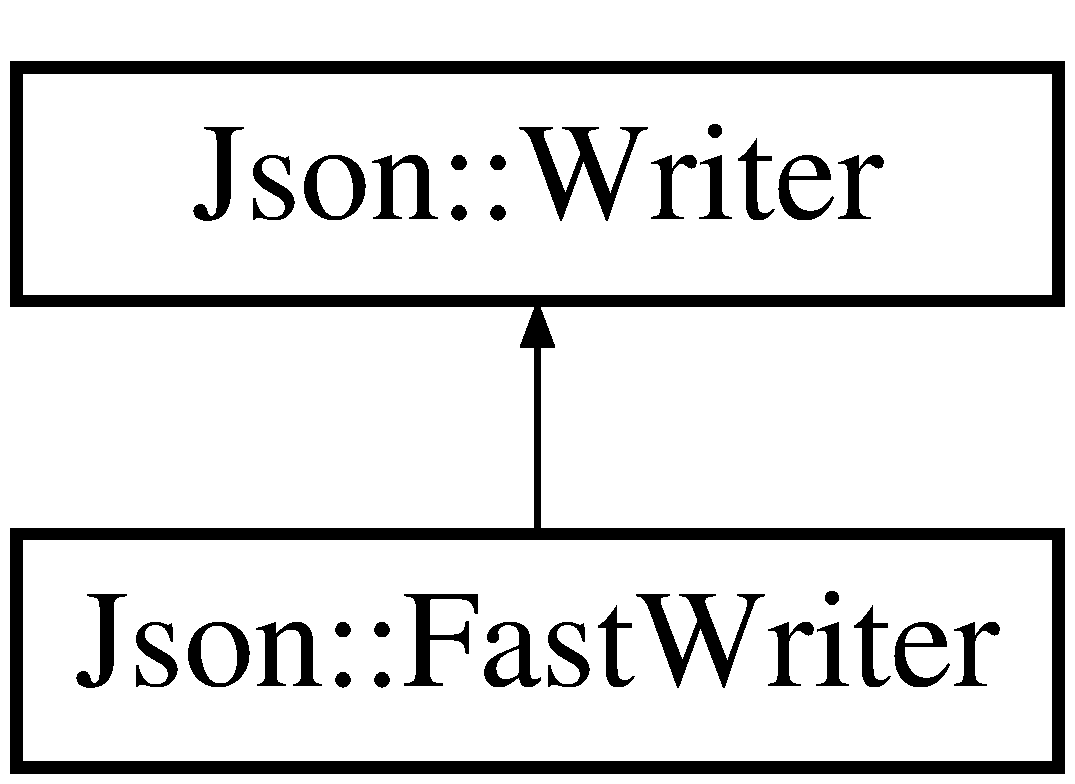
\includegraphics[height=2.000000cm]{classJson_1_1FastWriter}
\end{center}
\end{figure}
\subsection*{Public Member Functions}
\begin{DoxyCompactItemize}
\item 
void {\bfseries enable\+Y\+A\+M\+L\+Compatibility} ()\hypertarget{classJson_1_1FastWriter_a78d98e9f76d33660ad6e6a1abe287d45}{}\label{classJson_1_1FastWriter_a78d98e9f76d33660ad6e6a1abe287d45}

\item 
void \hyperlink{classJson_1_1FastWriter_a6e93d8dce951e408517311026a065b40}{drop\+Null\+Placeholders} ()\hypertarget{classJson_1_1FastWriter_a6e93d8dce951e408517311026a065b40}{}\label{classJson_1_1FastWriter_a6e93d8dce951e408517311026a065b40}

\begin{DoxyCompactList}\small\item\em Drop the \char`\"{}null\char`\"{} string from the writer\textquotesingle{}s output for null\+Values. Strictly speaking, this is not valid J\+S\+ON. But when the output is being fed to a browser\textquotesingle{}s Javascript, it makes for smaller output and the browser can handle the output just fine. \end{DoxyCompactList}\item 
void {\bfseries omit\+Ending\+Line\+Feed} ()\hypertarget{classJson_1_1FastWriter_af4ee077d365d75941fb2688d97207a55}{}\label{classJson_1_1FastWriter_af4ee077d365d75941fb2688d97207a55}

\item 
J\+S\+O\+N\+C\+P\+P\+\_\+\+S\+T\+R\+I\+NG {\bfseries write} (const \hyperlink{classJson_1_1Value}{Value} \&root) J\+S\+O\+N\+C\+P\+P\+\_\+\+O\+V\+E\+R\+R\+I\+DE\hypertarget{classJson_1_1FastWriter_a93d45ba4bc312371d08beb3e3dfbe654}{}\label{classJson_1_1FastWriter_a93d45ba4bc312371d08beb3e3dfbe654}

\end{DoxyCompactItemize}


\subsection{Detailed Description}
Outputs a \hyperlink{classJson_1_1Value}{Value} in \href{http://www.json.org}{\tt J\+S\+ON} format without formatting (not human friendly). 

The J\+S\+ON document is written in a single line. It is not intended for \textquotesingle{}human\textquotesingle{} consumption, but may be usefull to support feature such as R\+PC where bandwith is limited. \begin{DoxySeeAlso}{See also}
\hyperlink{classJson_1_1Reader}{Reader}, \hyperlink{classJson_1_1Value}{Value} 
\end{DoxySeeAlso}
\begin{DoxyRefDesc}{Deprecated}
\item[\hyperlink{deprecated__deprecated000008}{Deprecated}]Use \hyperlink{classJson_1_1StreamWriterBuilder}{Stream\+Writer\+Builder}. \end{DoxyRefDesc}


The documentation for this class was generated from the following files\+:\begin{DoxyCompactItemize}
\item 
Appserver/src/external/json/json.\+h\item 
Appserver/src/external/json/jsoncpp.\+cpp\end{DoxyCompactItemize}

\hypertarget{classfbson_1_1FbsonWriterT}{}\section{fbson\+:\+:Fbson\+WriterT$<$ T $>$ Class Template Reference}
\label{classfbson_1_1FbsonWriterT}\index{fbson\+::\+Fbson\+Writer\+T$<$ T $>$@{fbson\+::\+Fbson\+Writer\+T$<$ T $>$}}


The documentation for this class was generated from the following file\+:\begin{DoxyCompactItemize}
\item 
Appserver/src/external/rocksdb/utilities/json\+\_\+document.\+h\end{DoxyCompactItemize}

\hypertarget{classJson_1_1Features}{}\section{Json\+:\+:Features Class Reference}
\label{classJson_1_1Features}\index{Json\+::\+Features@{Json\+::\+Features}}


Configuration passed to reader and writer. This configuration object can be used to force the \hyperlink{classJson_1_1Reader}{Reader} or \hyperlink{classJson_1_1Writer}{Writer} to behave in a standard conforming way.  




{\ttfamily \#include $<$json.\+h$>$}

\subsection*{Public Member Functions}
\begin{DoxyCompactItemize}
\item 
\hyperlink{classJson_1_1Features_ad15a091cb61bb31323299a95970d2644}{Features} ()\hypertarget{classJson_1_1Features_ad15a091cb61bb31323299a95970d2644}{}\label{classJson_1_1Features_ad15a091cb61bb31323299a95970d2644}

\begin{DoxyCompactList}\small\item\em Initialize the configuration like Json\+Config\+::all\+Features;. \end{DoxyCompactList}\end{DoxyCompactItemize}
\subsection*{Static Public Member Functions}
\begin{DoxyCompactItemize}
\item 
static \hyperlink{classJson_1_1Features}{Features} \hyperlink{classJson_1_1Features_a63894da6e2c100b38741fa933f3d33ae}{all} ()
\begin{DoxyCompactList}\small\item\em A configuration that allows all features and assumes all strings are U\+T\+F-\/8. \end{DoxyCompactList}\item 
static \hyperlink{classJson_1_1Features}{Features} \hyperlink{classJson_1_1Features_ae23176c14b2e79e81fb61fb1a8ab58ee}{strict\+Mode} ()
\begin{DoxyCompactList}\small\item\em A configuration that is strictly compatible with the J\+S\+ON specification. \end{DoxyCompactList}\end{DoxyCompactItemize}
\subsection*{Public Attributes}
\begin{DoxyCompactItemize}
\item 
bool \hyperlink{classJson_1_1Features_a33afd389719624b6bdb23950b3c346c9}{allow\+Comments\+\_\+}\hypertarget{classJson_1_1Features_a33afd389719624b6bdb23950b3c346c9}{}\label{classJson_1_1Features_a33afd389719624b6bdb23950b3c346c9}

\begin{DoxyCompactList}\small\item\em {\ttfamily true} if comments are allowed. Default\+: {\ttfamily true}. \end{DoxyCompactList}\item 
bool \hyperlink{classJson_1_1Features_a1162c37a1458adc32582b585b552f9c3}{strict\+Root\+\_\+}
\item 
bool \hyperlink{classJson_1_1Features_a5076aa72c05c7596ac339ede36c97a6a}{allow\+Dropped\+Null\+Placeholders\+\_\+}\hypertarget{classJson_1_1Features_a5076aa72c05c7596ac339ede36c97a6a}{}\label{classJson_1_1Features_a5076aa72c05c7596ac339ede36c97a6a}

\begin{DoxyCompactList}\small\item\em {\ttfamily true} if dropped null placeholders are allowed. Default\+: {\ttfamily false}. \end{DoxyCompactList}\item 
bool \hyperlink{classJson_1_1Features_aff3cb16b79d15d3d761b11a0dd6d4d6b}{allow\+Numeric\+Keys\+\_\+}\hypertarget{classJson_1_1Features_aff3cb16b79d15d3d761b11a0dd6d4d6b}{}\label{classJson_1_1Features_aff3cb16b79d15d3d761b11a0dd6d4d6b}

\begin{DoxyCompactList}\small\item\em {\ttfamily true} if numeric object key are allowed. Default\+: {\ttfamily false}. \end{DoxyCompactList}\end{DoxyCompactItemize}


\subsection{Detailed Description}
Configuration passed to reader and writer. This configuration object can be used to force the \hyperlink{classJson_1_1Reader}{Reader} or \hyperlink{classJson_1_1Writer}{Writer} to behave in a standard conforming way. 

\subsection{Member Function Documentation}
\index{Json\+::\+Features@{Json\+::\+Features}!all@{all}}
\index{all@{all}!Json\+::\+Features@{Json\+::\+Features}}
\subsubsection[{\texorpdfstring{all()}{all()}}]{\setlength{\rightskip}{0pt plus 5cm}{\bf Features} Json\+::\+Features\+::all (
\begin{DoxyParamCaption}
{}
\end{DoxyParamCaption}
)\hspace{0.3cm}{\ttfamily [static]}}\hypertarget{classJson_1_1Features_a63894da6e2c100b38741fa933f3d33ae}{}\label{classJson_1_1Features_a63894da6e2c100b38741fa933f3d33ae}


A configuration that allows all features and assumes all strings are U\+T\+F-\/8. 


\begin{DoxyItemize}
\item C \& C++ comments are allowed
\item Root object can be any J\+S\+ON value
\item Assumes \hyperlink{classJson_1_1Value}{Value} strings are encoded in U\+T\+F-\/8 
\end{DoxyItemize}\index{Json\+::\+Features@{Json\+::\+Features}!strict\+Mode@{strict\+Mode}}
\index{strict\+Mode@{strict\+Mode}!Json\+::\+Features@{Json\+::\+Features}}
\subsubsection[{\texorpdfstring{strict\+Mode()}{strictMode()}}]{\setlength{\rightskip}{0pt plus 5cm}{\bf Features} Json\+::\+Features\+::strict\+Mode (
\begin{DoxyParamCaption}
{}
\end{DoxyParamCaption}
)\hspace{0.3cm}{\ttfamily [static]}}\hypertarget{classJson_1_1Features_ae23176c14b2e79e81fb61fb1a8ab58ee}{}\label{classJson_1_1Features_ae23176c14b2e79e81fb61fb1a8ab58ee}


A configuration that is strictly compatible with the J\+S\+ON specification. 


\begin{DoxyItemize}
\item Comments are forbidden.
\item Root object must be either an array or an object value.
\item Assumes \hyperlink{classJson_1_1Value}{Value} strings are encoded in U\+T\+F-\/8 
\end{DoxyItemize}

\subsection{Member Data Documentation}
\index{Json\+::\+Features@{Json\+::\+Features}!strict\+Root\+\_\+@{strict\+Root\+\_\+}}
\index{strict\+Root\+\_\+@{strict\+Root\+\_\+}!Json\+::\+Features@{Json\+::\+Features}}
\subsubsection[{\texorpdfstring{strict\+Root\+\_\+}{strictRoot\_}}]{\setlength{\rightskip}{0pt plus 5cm}bool Json\+::\+Features\+::strict\+Root\+\_\+}\hypertarget{classJson_1_1Features_a1162c37a1458adc32582b585b552f9c3}{}\label{classJson_1_1Features_a1162c37a1458adc32582b585b552f9c3}
{\ttfamily true} if root must be either an array or an object value. Default\+: {\ttfamily false}. 

The documentation for this class was generated from the following files\+:\begin{DoxyCompactItemize}
\item 
Appserver/src/external/json/json.\+h\item 
Appserver/src/external/json/jsoncpp.\+cpp\end{DoxyCompactItemize}

\hypertarget{classrocksdb_1_1spatial_1_1FeatureSet}{}\section{rocksdb\+:\+:spatial\+:\+:Feature\+Set Class Reference}
\label{classrocksdb_1_1spatial_1_1FeatureSet}\index{rocksdb\+::spatial\+::\+Feature\+Set@{rocksdb\+::spatial\+::\+Feature\+Set}}
\subsection*{Classes}
\begin{DoxyCompactItemize}
\item 
class \hyperlink{classrocksdb_1_1spatial_1_1FeatureSet_1_1iterator}{iterator}
\end{DoxyCompactItemize}
\subsection*{Public Member Functions}
\begin{DoxyCompactItemize}
\item 
\hyperlink{classrocksdb_1_1spatial_1_1FeatureSet}{Feature\+Set} $\ast$ {\bfseries Set} (const std\+::string \&key, const \hyperlink{structrocksdb_1_1spatial_1_1Variant}{Variant} \&value)\hypertarget{classrocksdb_1_1spatial_1_1FeatureSet_ab1416a40ee4aa9f7c819f5bf494f1762}{}\label{classrocksdb_1_1spatial_1_1FeatureSet_ab1416a40ee4aa9f7c819f5bf494f1762}

\item 
bool {\bfseries Contains} (const std\+::string \&key) const\hypertarget{classrocksdb_1_1spatial_1_1FeatureSet_a19e5279469b2e40834574d0f57bf1e94}{}\label{classrocksdb_1_1spatial_1_1FeatureSet_a19e5279469b2e40834574d0f57bf1e94}

\item 
const \hyperlink{structrocksdb_1_1spatial_1_1Variant}{Variant} \& {\bfseries Get} (const std\+::string \&key) const\hypertarget{classrocksdb_1_1spatial_1_1FeatureSet_a075c3377db58666af33b58fd48e3ddfd}{}\label{classrocksdb_1_1spatial_1_1FeatureSet_a075c3377db58666af33b58fd48e3ddfd}

\item 
\hyperlink{classrocksdb_1_1spatial_1_1FeatureSet_1_1iterator}{iterator} {\bfseries Find} (const std\+::string \&key) const\hypertarget{classrocksdb_1_1spatial_1_1FeatureSet_a6b31f38d98f78adcddec19b82165e130}{}\label{classrocksdb_1_1spatial_1_1FeatureSet_a6b31f38d98f78adcddec19b82165e130}

\item 
\hyperlink{classrocksdb_1_1spatial_1_1FeatureSet_1_1iterator}{iterator} {\bfseries begin} () const\hypertarget{classrocksdb_1_1spatial_1_1FeatureSet_ab16c975d8d615b19302bb78c1a799d9d}{}\label{classrocksdb_1_1spatial_1_1FeatureSet_ab16c975d8d615b19302bb78c1a799d9d}

\item 
\hyperlink{classrocksdb_1_1spatial_1_1FeatureSet_1_1iterator}{iterator} {\bfseries end} () const\hypertarget{classrocksdb_1_1spatial_1_1FeatureSet_abd40d3c0d1c6bd13b033d47b1f39cef5}{}\label{classrocksdb_1_1spatial_1_1FeatureSet_abd40d3c0d1c6bd13b033d47b1f39cef5}

\item 
void {\bfseries Clear} ()\hypertarget{classrocksdb_1_1spatial_1_1FeatureSet_a369a34f1241cbe608f7aaa04aa09ccc2}{}\label{classrocksdb_1_1spatial_1_1FeatureSet_a369a34f1241cbe608f7aaa04aa09ccc2}

\item 
size\+\_\+t {\bfseries Size} () const\hypertarget{classrocksdb_1_1spatial_1_1FeatureSet_a362d81e1bba4d94dfb6afdfad999fe03}{}\label{classrocksdb_1_1spatial_1_1FeatureSet_a362d81e1bba4d94dfb6afdfad999fe03}

\item 
void {\bfseries Serialize} (std\+::string $\ast$output) const\hypertarget{classrocksdb_1_1spatial_1_1FeatureSet_a1ecf6e07872b0b9b074ede1b6e7542f3}{}\label{classrocksdb_1_1spatial_1_1FeatureSet_a1ecf6e07872b0b9b074ede1b6e7542f3}

\item 
bool {\bfseries Deserialize} (const \hyperlink{classrocksdb_1_1Slice}{Slice} \&input)\hypertarget{classrocksdb_1_1spatial_1_1FeatureSet_a4b4e2a21b58261fbe09b2c5753463ad3}{}\label{classrocksdb_1_1spatial_1_1FeatureSet_a4b4e2a21b58261fbe09b2c5753463ad3}

\item 
std\+::string {\bfseries Debug\+String} () const\hypertarget{classrocksdb_1_1spatial_1_1FeatureSet_a08fd09258a3ec53d0c13f6c1c21b8aa9}{}\label{classrocksdb_1_1spatial_1_1FeatureSet_a08fd09258a3ec53d0c13f6c1c21b8aa9}

\end{DoxyCompactItemize}


The documentation for this class was generated from the following file\+:\begin{DoxyCompactItemize}
\item 
Appserver/src/external/rocksdb/utilities/spatial\+\_\+db.\+h\end{DoxyCompactItemize}

\hypertarget{structrocksdb_1_1Env_1_1FileAttributes}{}\section{rocksdb\+:\+:Env\+:\+:File\+Attributes Struct Reference}
\label{structrocksdb_1_1Env_1_1FileAttributes}\index{rocksdb\+::\+Env\+::\+File\+Attributes@{rocksdb\+::\+Env\+::\+File\+Attributes}}
\subsection*{Public Attributes}
\begin{DoxyCompactItemize}
\item 
std\+::string {\bfseries name}\hypertarget{structrocksdb_1_1Env_1_1FileAttributes_a5162ac457df2626f8aad0e2d088c5c46}{}\label{structrocksdb_1_1Env_1_1FileAttributes_a5162ac457df2626f8aad0e2d088c5c46}

\item 
uint64\+\_\+t {\bfseries size\+\_\+bytes}\hypertarget{structrocksdb_1_1Env_1_1FileAttributes_afd58487fad455d8bc93229fa52fca9c6}{}\label{structrocksdb_1_1Env_1_1FileAttributes_afd58487fad455d8bc93229fa52fca9c6}

\end{DoxyCompactItemize}


The documentation for this struct was generated from the following file\+:\begin{DoxyCompactItemize}
\item 
Appserver/src/external/rocksdb/env.\+h\end{DoxyCompactItemize}

\hypertarget{classrocksdb_1_1FileLock}{}\section{rocksdb\+:\+:File\+Lock Class Reference}
\label{classrocksdb_1_1FileLock}\index{rocksdb\+::\+File\+Lock@{rocksdb\+::\+File\+Lock}}
Inheritance diagram for rocksdb\+:\+:File\+Lock\+:\begin{figure}[H]
\begin{center}
\leavevmode
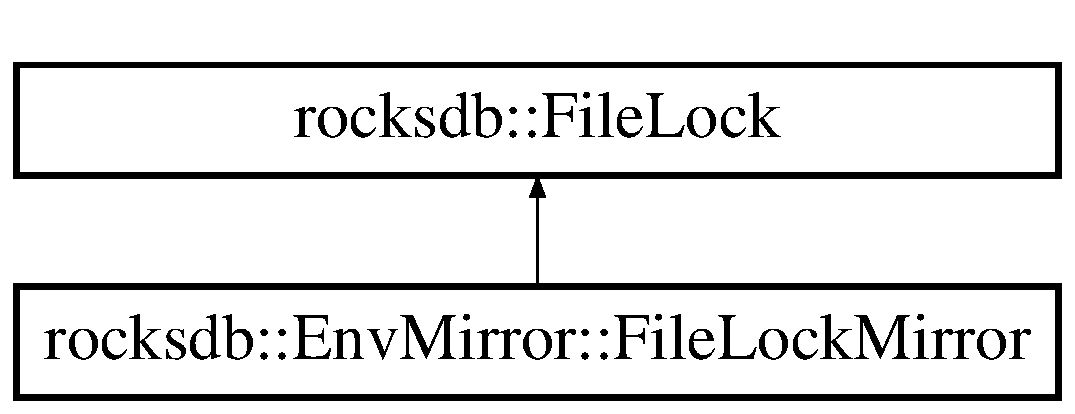
\includegraphics[height=2.000000cm]{classrocksdb_1_1FileLock}
\end{center}
\end{figure}


The documentation for this class was generated from the following file\+:\begin{DoxyCompactItemize}
\item 
Appserver/src/external/rocksdb/env.\+h\end{DoxyCompactItemize}

\hypertarget{classrocksdb_1_1EnvMirror_1_1FileLockMirror}{}\section{rocksdb\+:\+:Env\+Mirror\+:\+:File\+Lock\+Mirror Class Reference}
\label{classrocksdb_1_1EnvMirror_1_1FileLockMirror}\index{rocksdb\+::\+Env\+Mirror\+::\+File\+Lock\+Mirror@{rocksdb\+::\+Env\+Mirror\+::\+File\+Lock\+Mirror}}
Inheritance diagram for rocksdb\+:\+:Env\+Mirror\+:\+:File\+Lock\+Mirror\+:\begin{figure}[H]
\begin{center}
\leavevmode
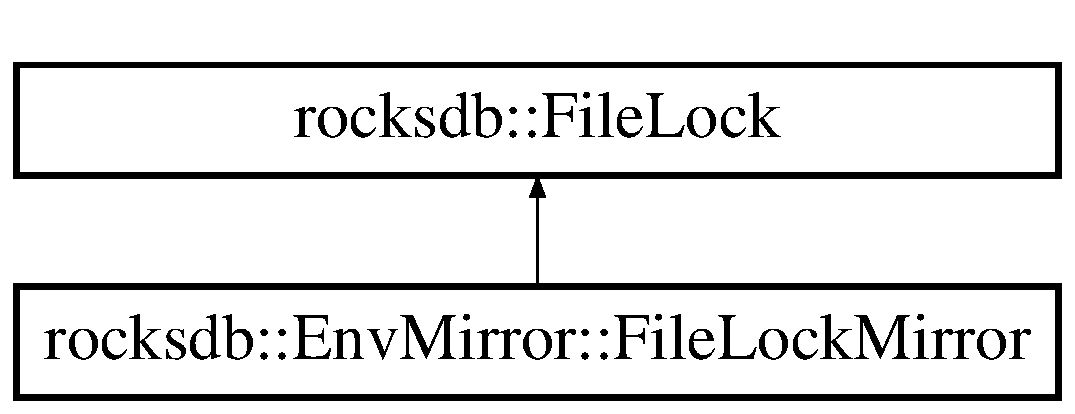
\includegraphics[height=2.000000cm]{classrocksdb_1_1EnvMirror_1_1FileLockMirror}
\end{center}
\end{figure}
\subsection*{Public Member Functions}
\begin{DoxyCompactItemize}
\item 
{\bfseries File\+Lock\+Mirror} (\hyperlink{classrocksdb_1_1FileLock}{File\+Lock} $\ast$a, \hyperlink{classrocksdb_1_1FileLock}{File\+Lock} $\ast$b)\hypertarget{classrocksdb_1_1EnvMirror_1_1FileLockMirror_ada51022b02a97f0a72b7b79416bbae44}{}\label{classrocksdb_1_1EnvMirror_1_1FileLockMirror_ada51022b02a97f0a72b7b79416bbae44}

\end{DoxyCompactItemize}
\subsection*{Public Attributes}
\begin{DoxyCompactItemize}
\item 
\hyperlink{classrocksdb_1_1FileLock}{File\+Lock} $\ast$ {\bfseries a\+\_\+}\hypertarget{classrocksdb_1_1EnvMirror_1_1FileLockMirror_a535762d761699ce90fd9051b58f4d275}{}\label{classrocksdb_1_1EnvMirror_1_1FileLockMirror_a535762d761699ce90fd9051b58f4d275}

\item 
\hyperlink{classrocksdb_1_1FileLock}{File\+Lock} $\ast$ {\bfseries b\+\_\+}\hypertarget{classrocksdb_1_1EnvMirror_1_1FileLockMirror_a611b7e46ab9cbea5e8fee68258f3031a}{}\label{classrocksdb_1_1EnvMirror_1_1FileLockMirror_a611b7e46ab9cbea5e8fee68258f3031a}

\end{DoxyCompactItemize}


The documentation for this class was generated from the following file\+:\begin{DoxyCompactItemize}
\item 
Appserver/src/external/rocksdb/utilities/env\+\_\+mirror.\+h\end{DoxyCompactItemize}

\hypertarget{classrocksdb_1_1FilterBitsBuilder}{}\section{rocksdb\+:\+:Filter\+Bits\+Builder Class Reference}
\label{classrocksdb_1_1FilterBitsBuilder}\index{rocksdb\+::\+Filter\+Bits\+Builder@{rocksdb\+::\+Filter\+Bits\+Builder}}
\subsection*{Public Member Functions}
\begin{DoxyCompactItemize}
\item 
virtual void {\bfseries Add\+Key} (const \hyperlink{classrocksdb_1_1Slice}{Slice} \&key)=0\hypertarget{classrocksdb_1_1FilterBitsBuilder_a527b3622ef1abcd29843da3968f954ea}{}\label{classrocksdb_1_1FilterBitsBuilder_a527b3622ef1abcd29843da3968f954ea}

\item 
virtual \hyperlink{classrocksdb_1_1Slice}{Slice} {\bfseries Finish} (std\+::unique\+\_\+ptr$<$ const char\mbox{[}$\,$\mbox{]}$>$ $\ast$buf)=0\hypertarget{classrocksdb_1_1FilterBitsBuilder_a09d3d61df0da3b9c70b8e10f42794718}{}\label{classrocksdb_1_1FilterBitsBuilder_a09d3d61df0da3b9c70b8e10f42794718}

\end{DoxyCompactItemize}


The documentation for this class was generated from the following file\+:\begin{DoxyCompactItemize}
\item 
Appserver/src/external/rocksdb/filter\+\_\+policy.\+h\end{DoxyCompactItemize}

\hypertarget{classrocksdb_1_1FilterBitsReader}{}\section{rocksdb\+:\+:Filter\+Bits\+Reader Class Reference}
\label{classrocksdb_1_1FilterBitsReader}\index{rocksdb\+::\+Filter\+Bits\+Reader@{rocksdb\+::\+Filter\+Bits\+Reader}}
\subsection*{Public Member Functions}
\begin{DoxyCompactItemize}
\item 
virtual bool {\bfseries May\+Match} (const \hyperlink{classrocksdb_1_1Slice}{Slice} \&entry)=0\hypertarget{classrocksdb_1_1FilterBitsReader_a0cd48328c31812cfc82c472416bff4df}{}\label{classrocksdb_1_1FilterBitsReader_a0cd48328c31812cfc82c472416bff4df}

\end{DoxyCompactItemize}


The documentation for this class was generated from the following file\+:\begin{DoxyCompactItemize}
\item 
Appserver/src/external/rocksdb/filter\+\_\+policy.\+h\end{DoxyCompactItemize}

\hypertarget{classrocksdb_1_1FilterPolicy}{}\section{rocksdb\+:\+:Filter\+Policy Class Reference}
\label{classrocksdb_1_1FilterPolicy}\index{rocksdb\+::\+Filter\+Policy@{rocksdb\+::\+Filter\+Policy}}
\subsection*{Public Member Functions}
\begin{DoxyCompactItemize}
\item 
virtual const char $\ast$ {\bfseries Name} () const =0\hypertarget{classrocksdb_1_1FilterPolicy_a51521763e767376e3325e5565a6f7bf6}{}\label{classrocksdb_1_1FilterPolicy_a51521763e767376e3325e5565a6f7bf6}

\item 
virtual void {\bfseries Create\+Filter} (const \hyperlink{classrocksdb_1_1Slice}{Slice} $\ast$keys, int n, std\+::string $\ast$dst) const =0\hypertarget{classrocksdb_1_1FilterPolicy_ad43c700719f38ca4ef864ffb3ec73f5e}{}\label{classrocksdb_1_1FilterPolicy_ad43c700719f38ca4ef864ffb3ec73f5e}

\item 
virtual bool {\bfseries Key\+May\+Match} (const \hyperlink{classrocksdb_1_1Slice}{Slice} \&key, const \hyperlink{classrocksdb_1_1Slice}{Slice} \&filter) const =0\hypertarget{classrocksdb_1_1FilterPolicy_afd9296968a61335cc7e1eb5ae6f85489}{}\label{classrocksdb_1_1FilterPolicy_afd9296968a61335cc7e1eb5ae6f85489}

\item 
virtual \hyperlink{classrocksdb_1_1FilterBitsBuilder}{Filter\+Bits\+Builder} $\ast$ {\bfseries Get\+Filter\+Bits\+Builder} () const\hypertarget{classrocksdb_1_1FilterPolicy_a267639ad348889203f98af1fc60286d7}{}\label{classrocksdb_1_1FilterPolicy_a267639ad348889203f98af1fc60286d7}

\item 
virtual \hyperlink{classrocksdb_1_1FilterBitsReader}{Filter\+Bits\+Reader} $\ast$ {\bfseries Get\+Filter\+Bits\+Reader} (const \hyperlink{classrocksdb_1_1Slice}{Slice} \&contents) const\hypertarget{classrocksdb_1_1FilterPolicy_abb583d453b4e3d158d0f329e7724a15e}{}\label{classrocksdb_1_1FilterPolicy_abb583d453b4e3d158d0f329e7724a15e}

\end{DoxyCompactItemize}


The documentation for this class was generated from the following file\+:\begin{DoxyCompactItemize}
\item 
Appserver/src/external/rocksdb/filter\+\_\+policy.\+h\end{DoxyCompactItemize}

\hypertarget{classrocksdb_1_1FlushBlockBySizePolicyFactory}{}\section{rocksdb\+:\+:Flush\+Block\+By\+Size\+Policy\+Factory Class Reference}
\label{classrocksdb_1_1FlushBlockBySizePolicyFactory}\index{rocksdb\+::\+Flush\+Block\+By\+Size\+Policy\+Factory@{rocksdb\+::\+Flush\+Block\+By\+Size\+Policy\+Factory}}
Inheritance diagram for rocksdb\+:\+:Flush\+Block\+By\+Size\+Policy\+Factory\+:\begin{figure}[H]
\begin{center}
\leavevmode
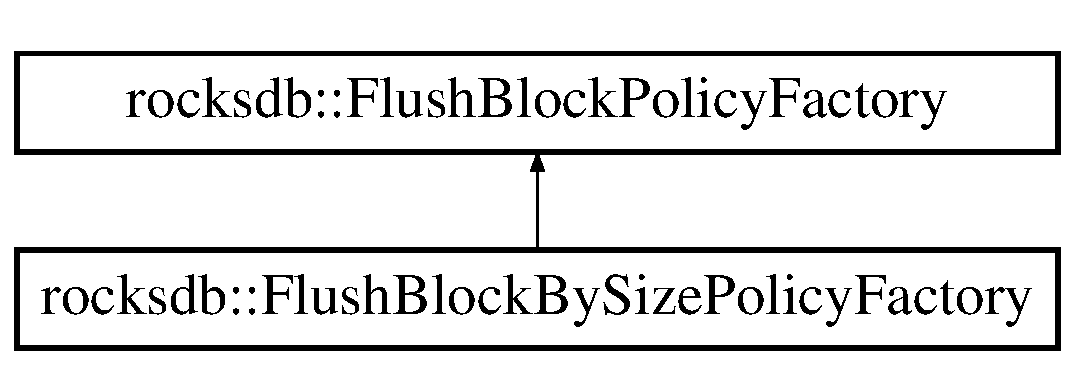
\includegraphics[height=2.000000cm]{classrocksdb_1_1FlushBlockBySizePolicyFactory}
\end{center}
\end{figure}
\subsection*{Public Member Functions}
\begin{DoxyCompactItemize}
\item 
virtual const char $\ast$ {\bfseries Name} () const override\hypertarget{classrocksdb_1_1FlushBlockBySizePolicyFactory_a09a206a61a35e976089c479c1af12f1f}{}\label{classrocksdb_1_1FlushBlockBySizePolicyFactory_a09a206a61a35e976089c479c1af12f1f}

\item 
virtual \hyperlink{classrocksdb_1_1FlushBlockPolicy}{Flush\+Block\+Policy} $\ast$ {\bfseries New\+Flush\+Block\+Policy} (const \hyperlink{structrocksdb_1_1BlockBasedTableOptions}{Block\+Based\+Table\+Options} \&table\+\_\+options, const Block\+Builder \&data\+\_\+block\+\_\+builder) const override\hypertarget{classrocksdb_1_1FlushBlockBySizePolicyFactory_aa4371099b2479df6259e2074f124434b}{}\label{classrocksdb_1_1FlushBlockBySizePolicyFactory_aa4371099b2479df6259e2074f124434b}

\end{DoxyCompactItemize}


The documentation for this class was generated from the following file\+:\begin{DoxyCompactItemize}
\item 
Appserver/src/external/rocksdb/flush\+\_\+block\+\_\+policy.\+h\end{DoxyCompactItemize}

\hypertarget{classrocksdb_1_1FlushBlockPolicy}{}\section{rocksdb\+:\+:Flush\+Block\+Policy Class Reference}
\label{classrocksdb_1_1FlushBlockPolicy}\index{rocksdb\+::\+Flush\+Block\+Policy@{rocksdb\+::\+Flush\+Block\+Policy}}
\subsection*{Public Member Functions}
\begin{DoxyCompactItemize}
\item 
virtual bool {\bfseries Update} (const \hyperlink{classrocksdb_1_1Slice}{Slice} \&key, const \hyperlink{classrocksdb_1_1Slice}{Slice} \&value)=0\hypertarget{classrocksdb_1_1FlushBlockPolicy_a12b20dcb03cadc7c43c8a29e8889fbea}{}\label{classrocksdb_1_1FlushBlockPolicy_a12b20dcb03cadc7c43c8a29e8889fbea}

\end{DoxyCompactItemize}


The documentation for this class was generated from the following file\+:\begin{DoxyCompactItemize}
\item 
Appserver/src/external/rocksdb/flush\+\_\+block\+\_\+policy.\+h\end{DoxyCompactItemize}

\hypertarget{classrocksdb_1_1FlushBlockPolicyFactory}{}\section{rocksdb\+:\+:Flush\+Block\+Policy\+Factory Class Reference}
\label{classrocksdb_1_1FlushBlockPolicyFactory}\index{rocksdb\+::\+Flush\+Block\+Policy\+Factory@{rocksdb\+::\+Flush\+Block\+Policy\+Factory}}
Inheritance diagram for rocksdb\+:\+:Flush\+Block\+Policy\+Factory\+:\begin{figure}[H]
\begin{center}
\leavevmode
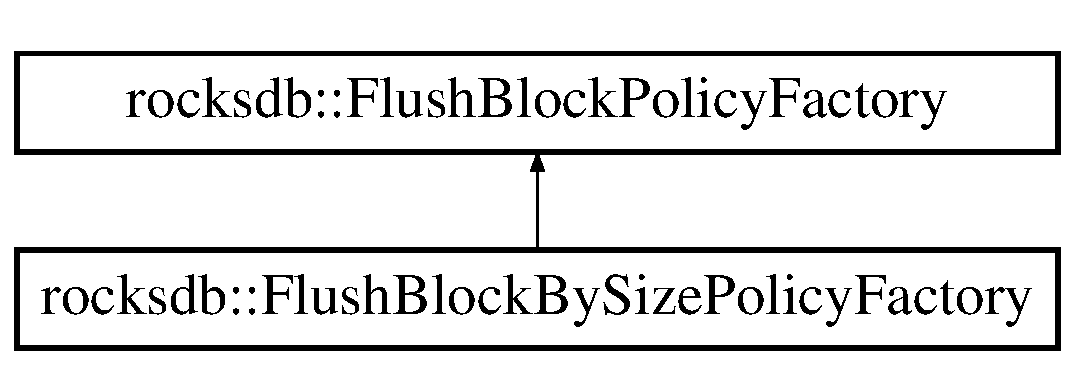
\includegraphics[height=2.000000cm]{classrocksdb_1_1FlushBlockPolicyFactory}
\end{center}
\end{figure}
\subsection*{Public Member Functions}
\begin{DoxyCompactItemize}
\item 
virtual const char $\ast$ {\bfseries Name} () const =0\hypertarget{classrocksdb_1_1FlushBlockPolicyFactory_ac47177388c186c65759cc1fd2d73a5f9}{}\label{classrocksdb_1_1FlushBlockPolicyFactory_ac47177388c186c65759cc1fd2d73a5f9}

\item 
virtual \hyperlink{classrocksdb_1_1FlushBlockPolicy}{Flush\+Block\+Policy} $\ast$ {\bfseries New\+Flush\+Block\+Policy} (const \hyperlink{structrocksdb_1_1BlockBasedTableOptions}{Block\+Based\+Table\+Options} \&table\+\_\+options, const Block\+Builder \&data\+\_\+block\+\_\+builder) const =0\hypertarget{classrocksdb_1_1FlushBlockPolicyFactory_ac4728294425869b3d0f81d15e43200b4}{}\label{classrocksdb_1_1FlushBlockPolicyFactory_ac4728294425869b3d0f81d15e43200b4}

\end{DoxyCompactItemize}


The documentation for this class was generated from the following file\+:\begin{DoxyCompactItemize}
\item 
Appserver/src/external/rocksdb/flush\+\_\+block\+\_\+policy.\+h\end{DoxyCompactItemize}

\hypertarget{structrocksdb_1_1FlushJobInfo}{}\section{rocksdb\+:\+:Flush\+Job\+Info Struct Reference}
\label{structrocksdb_1_1FlushJobInfo}\index{rocksdb\+::\+Flush\+Job\+Info@{rocksdb\+::\+Flush\+Job\+Info}}
\subsection*{Public Attributes}
\begin{DoxyCompactItemize}
\item 
std\+::string {\bfseries cf\+\_\+name}\hypertarget{structrocksdb_1_1FlushJobInfo_a924aca33916d216cdd3067503421b5c1}{}\label{structrocksdb_1_1FlushJobInfo_a924aca33916d216cdd3067503421b5c1}

\item 
std\+::string {\bfseries file\+\_\+path}\hypertarget{structrocksdb_1_1FlushJobInfo_a716b549513aa5fa49fd34ddc27d5ba28}{}\label{structrocksdb_1_1FlushJobInfo_a716b549513aa5fa49fd34ddc27d5ba28}

\item 
uint64\+\_\+t {\bfseries thread\+\_\+id}\hypertarget{structrocksdb_1_1FlushJobInfo_a165c4e1d14f6c0a3b6eb6f424dd5ab90}{}\label{structrocksdb_1_1FlushJobInfo_a165c4e1d14f6c0a3b6eb6f424dd5ab90}

\item 
int {\bfseries job\+\_\+id}\hypertarget{structrocksdb_1_1FlushJobInfo_aeaf78225922ab9cc0fb8a92013268ca9}{}\label{structrocksdb_1_1FlushJobInfo_aeaf78225922ab9cc0fb8a92013268ca9}

\item 
bool {\bfseries triggered\+\_\+writes\+\_\+slowdown}\hypertarget{structrocksdb_1_1FlushJobInfo_a22e452c6d1789f67ce0c4bf6fae8d0dd}{}\label{structrocksdb_1_1FlushJobInfo_a22e452c6d1789f67ce0c4bf6fae8d0dd}

\item 
bool {\bfseries triggered\+\_\+writes\+\_\+stop}\hypertarget{structrocksdb_1_1FlushJobInfo_a3d67070cf51b0121f738f0fca9b477a4}{}\label{structrocksdb_1_1FlushJobInfo_a3d67070cf51b0121f738f0fca9b477a4}

\item 
Sequence\+Number {\bfseries smallest\+\_\+seqno}\hypertarget{structrocksdb_1_1FlushJobInfo_a5a18e8dda289e2d23fd86944d422a8fc}{}\label{structrocksdb_1_1FlushJobInfo_a5a18e8dda289e2d23fd86944d422a8fc}

\item 
Sequence\+Number {\bfseries largest\+\_\+seqno}\hypertarget{structrocksdb_1_1FlushJobInfo_a2383fd356aa550a3db4def8ee3e9a2b6}{}\label{structrocksdb_1_1FlushJobInfo_a2383fd356aa550a3db4def8ee3e9a2b6}

\item 
\hyperlink{structrocksdb_1_1TableProperties}{Table\+Properties} {\bfseries table\+\_\+properties}\hypertarget{structrocksdb_1_1FlushJobInfo_a0ca795765af7fb79bdf9400fd6009b05}{}\label{structrocksdb_1_1FlushJobInfo_a0ca795765af7fb79bdf9400fd6009b05}

\end{DoxyCompactItemize}


The documentation for this struct was generated from the following file\+:\begin{DoxyCompactItemize}
\item 
Appserver/src/external/rocksdb/listener.\+h\end{DoxyCompactItemize}

\hypertarget{structrocksdb_1_1FlushOptions}{}\section{rocksdb\+:\+:Flush\+Options Struct Reference}
\label{structrocksdb_1_1FlushOptions}\index{rocksdb\+::\+Flush\+Options@{rocksdb\+::\+Flush\+Options}}
\subsection*{Public Attributes}
\begin{DoxyCompactItemize}
\item 
bool {\bfseries wait}\hypertarget{structrocksdb_1_1FlushOptions_af97da606e667aa0b4db459515c00ec3b}{}\label{structrocksdb_1_1FlushOptions_af97da606e667aa0b4db459515c00ec3b}

\end{DoxyCompactItemize}


The documentation for this struct was generated from the following file\+:\begin{DoxyCompactItemize}
\item 
Appserver/src/external/rocksdb/options.\+h\end{DoxyCompactItemize}

\hypertarget{structfrozen}{}\section{frozen Struct Reference}
\label{structfrozen}\index{frozen@{frozen}}
\subsection*{Public Attributes}
\begin{DoxyCompactItemize}
\item 
const char $\ast$ {\bfseries end}\hypertarget{structfrozen_a262986511243893cb6d0c424a533da6e}{}\label{structfrozen_a262986511243893cb6d0c424a533da6e}

\item 
const char $\ast$ {\bfseries cur}\hypertarget{structfrozen_a3a7cf08b9ba2b16d9c31be9c7ec65cb2}{}\label{structfrozen_a3a7cf08b9ba2b16d9c31be9c7ec65cb2}

\item 
struct \hyperlink{structjson__token}{json\+\_\+token} $\ast$ {\bfseries tokens}\hypertarget{structfrozen_afc396df24f82640326ba74df00082729}{}\label{structfrozen_afc396df24f82640326ba74df00082729}

\item 
int {\bfseries max\+\_\+tokens}\hypertarget{structfrozen_aee94f69748176e6e79b81147e0eee896}{}\label{structfrozen_aee94f69748176e6e79b81147e0eee896}

\item 
int {\bfseries num\+\_\+tokens}\hypertarget{structfrozen_abaabb9c26246e03c6c8f5da00fbef4cf}{}\label{structfrozen_abaabb9c26246e03c6c8f5da00fbef4cf}

\item 
int {\bfseries do\+\_\+realloc}\hypertarget{structfrozen_ac5827a169232910711a7db323eaa6aef}{}\label{structfrozen_ac5827a169232910711a7db323eaa6aef}

\end{DoxyCompactItemize}


The documentation for this struct was generated from the following file\+:\begin{DoxyCompactItemize}
\item 
Appserver/src/external/mongoose/mongoose.\+c\end{DoxyCompactItemize}

\hypertarget{classrocksdb_1_1GeoDB}{}\section{rocksdb\+:\+:Geo\+DB Class Reference}
\label{classrocksdb_1_1GeoDB}\index{rocksdb\+::\+Geo\+DB@{rocksdb\+::\+Geo\+DB}}
Inheritance diagram for rocksdb\+:\+:Geo\+DB\+:\begin{figure}[H]
\begin{center}
\leavevmode
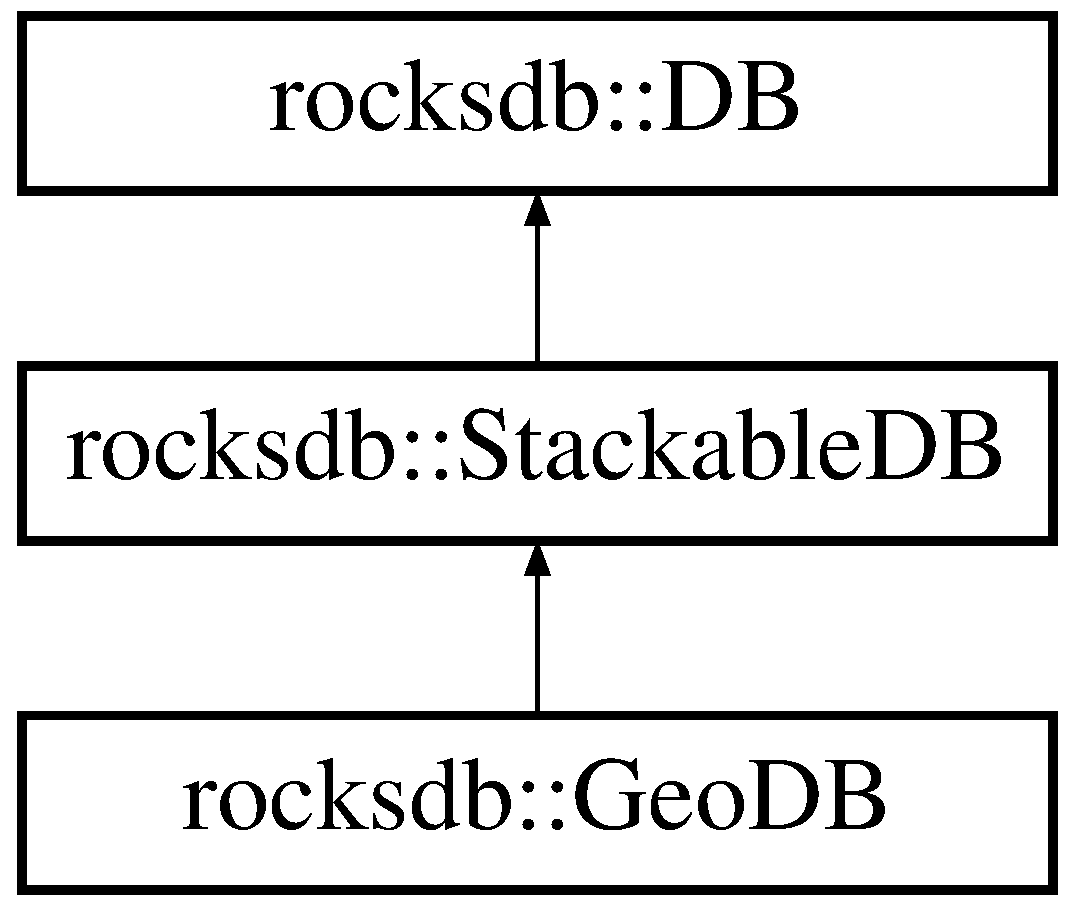
\includegraphics[height=3.000000cm]{classrocksdb_1_1GeoDB}
\end{center}
\end{figure}
\subsection*{Public Member Functions}
\begin{DoxyCompactItemize}
\item 
{\bfseries Geo\+DB} (\hyperlink{classrocksdb_1_1DB}{DB} $\ast$db, const \hyperlink{structrocksdb_1_1GeoDBOptions}{Geo\+D\+B\+Options} \&options)\hypertarget{classrocksdb_1_1GeoDB_aea4cdd1e86027b6126059e8eb2245c25}{}\label{classrocksdb_1_1GeoDB_aea4cdd1e86027b6126059e8eb2245c25}

\item 
virtual \hyperlink{classrocksdb_1_1Status}{Status} {\bfseries Insert} (const \hyperlink{classrocksdb_1_1GeoObject}{Geo\+Object} \&object)=0\hypertarget{classrocksdb_1_1GeoDB_a81c9e2268ccb793802cf44c69b1ea942}{}\label{classrocksdb_1_1GeoDB_a81c9e2268ccb793802cf44c69b1ea942}

\item 
virtual \hyperlink{classrocksdb_1_1Status}{Status} {\bfseries Get\+By\+Position} (const \hyperlink{classrocksdb_1_1GeoPosition}{Geo\+Position} \&pos, const \hyperlink{classrocksdb_1_1Slice}{Slice} \&id, std\+::string $\ast$value)=0\hypertarget{classrocksdb_1_1GeoDB_ac53062674afd942131c8503ace4e863c}{}\label{classrocksdb_1_1GeoDB_ac53062674afd942131c8503ace4e863c}

\item 
virtual \hyperlink{classrocksdb_1_1Status}{Status} {\bfseries Get\+By\+Id} (const \hyperlink{classrocksdb_1_1Slice}{Slice} \&id, \hyperlink{classrocksdb_1_1GeoObject}{Geo\+Object} $\ast$object)=0\hypertarget{classrocksdb_1_1GeoDB_a8f62bab51de989169f88875313323740}{}\label{classrocksdb_1_1GeoDB_a8f62bab51de989169f88875313323740}

\item 
virtual \hyperlink{classrocksdb_1_1Status}{Status} {\bfseries Remove} (const \hyperlink{classrocksdb_1_1Slice}{Slice} \&id)=0\hypertarget{classrocksdb_1_1GeoDB_a3079e4b1fe9f8da662f136b4bcf73354}{}\label{classrocksdb_1_1GeoDB_a3079e4b1fe9f8da662f136b4bcf73354}

\item 
virtual \hyperlink{classrocksdb_1_1GeoIterator}{Geo\+Iterator} $\ast$ {\bfseries Search\+Radial} (const \hyperlink{classrocksdb_1_1GeoPosition}{Geo\+Position} \&pos, double radius, int number\+\_\+of\+\_\+values=I\+N\+T\+\_\+\+M\+AX)=0\hypertarget{classrocksdb_1_1GeoDB_af7201ce086b3ceba0b6e0b7ba108a284}{}\label{classrocksdb_1_1GeoDB_af7201ce086b3ceba0b6e0b7ba108a284}

\end{DoxyCompactItemize}
\subsection*{Additional Inherited Members}


The documentation for this class was generated from the following file\+:\begin{DoxyCompactItemize}
\item 
Appserver/src/external/rocksdb/utilities/geo\+\_\+db.\+h\end{DoxyCompactItemize}

\hypertarget{structrocksdb_1_1GeoDBOptions}{}\section{rocksdb\+:\+:Geo\+D\+B\+Options Struct Reference}
\label{structrocksdb_1_1GeoDBOptions}\index{rocksdb\+::\+Geo\+D\+B\+Options@{rocksdb\+::\+Geo\+D\+B\+Options}}
\subsection*{Public Member Functions}
\begin{DoxyCompactItemize}
\item 
{\bfseries Geo\+D\+B\+Options} (\hyperlink{classrocksdb_1_1Logger}{Logger} $\ast$\+\_\+info\+\_\+log=nullptr)\hypertarget{structrocksdb_1_1GeoDBOptions_aae681ac7e6c94b79d597b86124ddea05}{}\label{structrocksdb_1_1GeoDBOptions_aae681ac7e6c94b79d597b86124ddea05}

\end{DoxyCompactItemize}
\subsection*{Public Attributes}
\begin{DoxyCompactItemize}
\item 
\hyperlink{classrocksdb_1_1Logger}{Logger} $\ast$ {\bfseries info\+\_\+log}\hypertarget{structrocksdb_1_1GeoDBOptions_aa26d74928c41e8bdfe2f52b1f1b7e3c4}{}\label{structrocksdb_1_1GeoDBOptions_aa26d74928c41e8bdfe2f52b1f1b7e3c4}

\end{DoxyCompactItemize}


The documentation for this struct was generated from the following file\+:\begin{DoxyCompactItemize}
\item 
Appserver/src/external/rocksdb/utilities/geo\+\_\+db.\+h\end{DoxyCompactItemize}

\hypertarget{classrocksdb_1_1GeoIterator}{}\section{rocksdb\+:\+:Geo\+Iterator Class Reference}
\label{classrocksdb_1_1GeoIterator}\index{rocksdb\+::\+Geo\+Iterator@{rocksdb\+::\+Geo\+Iterator}}
\subsection*{Public Member Functions}
\begin{DoxyCompactItemize}
\item 
virtual void {\bfseries Next} ()=0\hypertarget{classrocksdb_1_1GeoIterator_aea522ef4d34543506cd7249edc2ded26}{}\label{classrocksdb_1_1GeoIterator_aea522ef4d34543506cd7249edc2ded26}

\item 
virtual bool {\bfseries Valid} () const =0\hypertarget{classrocksdb_1_1GeoIterator_ae3894cef3836f41b5580aa195a1f2c83}{}\label{classrocksdb_1_1GeoIterator_ae3894cef3836f41b5580aa195a1f2c83}

\item 
virtual const \hyperlink{classrocksdb_1_1GeoObject}{Geo\+Object} \& {\bfseries geo\+\_\+object} ()=0\hypertarget{classrocksdb_1_1GeoIterator_adbf68aacb1401b97006a660b723488f5}{}\label{classrocksdb_1_1GeoIterator_adbf68aacb1401b97006a660b723488f5}

\item 
virtual \hyperlink{classrocksdb_1_1Status}{Status} {\bfseries status} () const =0\hypertarget{classrocksdb_1_1GeoIterator_a71220bc36b86557e1043dd2e8453b969}{}\label{classrocksdb_1_1GeoIterator_a71220bc36b86557e1043dd2e8453b969}

\end{DoxyCompactItemize}


The documentation for this class was generated from the following file\+:\begin{DoxyCompactItemize}
\item 
Appserver/src/external/rocksdb/utilities/geo\+\_\+db.\+h\end{DoxyCompactItemize}

\hypertarget{classrocksdb_1_1GeoObject}{}\section{rocksdb\+:\+:Geo\+Object Class Reference}
\label{classrocksdb_1_1GeoObject}\index{rocksdb\+::\+Geo\+Object@{rocksdb\+::\+Geo\+Object}}
\subsection*{Public Member Functions}
\begin{DoxyCompactItemize}
\item 
{\bfseries Geo\+Object} (const \hyperlink{classrocksdb_1_1GeoPosition}{Geo\+Position} \&pos, const std\+::string \&i, const std\+::string \&val)\hypertarget{classrocksdb_1_1GeoObject_a10df8c4ffca7b8bec3270202971f24fd}{}\label{classrocksdb_1_1GeoObject_a10df8c4ffca7b8bec3270202971f24fd}

\end{DoxyCompactItemize}
\subsection*{Public Attributes}
\begin{DoxyCompactItemize}
\item 
\hyperlink{classrocksdb_1_1GeoPosition}{Geo\+Position} {\bfseries position}\hypertarget{classrocksdb_1_1GeoObject_ad7a5bf0890a88078c0b78bb4f705e444}{}\label{classrocksdb_1_1GeoObject_ad7a5bf0890a88078c0b78bb4f705e444}

\item 
std\+::string {\bfseries id}\hypertarget{classrocksdb_1_1GeoObject_a0569d6274ab98445ef6ddc6222349003}{}\label{classrocksdb_1_1GeoObject_a0569d6274ab98445ef6ddc6222349003}

\item 
std\+::string {\bfseries value}\hypertarget{classrocksdb_1_1GeoObject_aadb5ce54d4e1e23e9649a32e695bd6f2}{}\label{classrocksdb_1_1GeoObject_aadb5ce54d4e1e23e9649a32e695bd6f2}

\end{DoxyCompactItemize}


The documentation for this class was generated from the following file\+:\begin{DoxyCompactItemize}
\item 
Appserver/src/external/rocksdb/utilities/geo\+\_\+db.\+h\end{DoxyCompactItemize}

\hypertarget{classrocksdb_1_1GeoPosition}{}\section{rocksdb\+:\+:Geo\+Position Class Reference}
\label{classrocksdb_1_1GeoPosition}\index{rocksdb\+::\+Geo\+Position@{rocksdb\+::\+Geo\+Position}}
\subsection*{Public Member Functions}
\begin{DoxyCompactItemize}
\item 
{\bfseries Geo\+Position} (double la=0, double lo=0)\hypertarget{classrocksdb_1_1GeoPosition_a2891539580cdc2d162d3861f785412b2}{}\label{classrocksdb_1_1GeoPosition_a2891539580cdc2d162d3861f785412b2}

\end{DoxyCompactItemize}
\subsection*{Public Attributes}
\begin{DoxyCompactItemize}
\item 
double {\bfseries latitude}\hypertarget{classrocksdb_1_1GeoPosition_aed89917cab50fcdc3b8e8ed38e9c9e6d}{}\label{classrocksdb_1_1GeoPosition_aed89917cab50fcdc3b8e8ed38e9c9e6d}

\item 
double {\bfseries longitude}\hypertarget{classrocksdb_1_1GeoPosition_a554149b696189e7fe8a622a51caa0f2a}{}\label{classrocksdb_1_1GeoPosition_a554149b696189e7fe8a622a51caa0f2a}

\end{DoxyCompactItemize}


The documentation for this class was generated from the following file\+:\begin{DoxyCompactItemize}
\item 
Appserver/src/external/rocksdb/utilities/geo\+\_\+db.\+h\end{DoxyCompactItemize}

\hypertarget{structrocksdb_1_1Cache_1_1Handle}{}\section{rocksdb\+:\+:Cache\+:\+:Handle Struct Reference}
\label{structrocksdb_1_1Cache_1_1Handle}\index{rocksdb\+::\+Cache\+::\+Handle@{rocksdb\+::\+Cache\+::\+Handle}}


The documentation for this struct was generated from the following file\+:\begin{DoxyCompactItemize}
\item 
Appserver/src/external/rocksdb/cache.\+h\end{DoxyCompactItemize}

\hypertarget{classrocksdb_1_1WriteBatch_1_1Handler}{}\section{rocksdb\+:\+:Write\+Batch\+:\+:Handler Class Reference}
\label{classrocksdb_1_1WriteBatch_1_1Handler}\index{rocksdb\+::\+Write\+Batch\+::\+Handler@{rocksdb\+::\+Write\+Batch\+::\+Handler}}
\subsection*{Public Member Functions}
\begin{DoxyCompactItemize}
\item 
virtual \hyperlink{classrocksdb_1_1Status}{Status} {\bfseries Put\+CF} (uint32\+\_\+t column\+\_\+family\+\_\+id, const \hyperlink{classrocksdb_1_1Slice}{Slice} \&key, const \hyperlink{classrocksdb_1_1Slice}{Slice} \&value)\hypertarget{classrocksdb_1_1WriteBatch_1_1Handler_a17e17f57d3d614483b3d849468db108a}{}\label{classrocksdb_1_1WriteBatch_1_1Handler_a17e17f57d3d614483b3d849468db108a}

\item 
virtual void {\bfseries Put} (const \hyperlink{classrocksdb_1_1Slice}{Slice} \&, const \hyperlink{classrocksdb_1_1Slice}{Slice} \&)\hypertarget{classrocksdb_1_1WriteBatch_1_1Handler_accf33beb9e1587846826c243302a0cdc}{}\label{classrocksdb_1_1WriteBatch_1_1Handler_accf33beb9e1587846826c243302a0cdc}

\item 
virtual \hyperlink{classrocksdb_1_1Status}{Status} {\bfseries Delete\+CF} (uint32\+\_\+t column\+\_\+family\+\_\+id, const \hyperlink{classrocksdb_1_1Slice}{Slice} \&key)\hypertarget{classrocksdb_1_1WriteBatch_1_1Handler_a055858a9b7c0479d15d909d4f1f6c125}{}\label{classrocksdb_1_1WriteBatch_1_1Handler_a055858a9b7c0479d15d909d4f1f6c125}

\item 
virtual void {\bfseries Delete} (const \hyperlink{classrocksdb_1_1Slice}{Slice} \&)\hypertarget{classrocksdb_1_1WriteBatch_1_1Handler_aa32531e83a34a1dd9da2a0e4bfb26e1e}{}\label{classrocksdb_1_1WriteBatch_1_1Handler_aa32531e83a34a1dd9da2a0e4bfb26e1e}

\item 
virtual \hyperlink{classrocksdb_1_1Status}{Status} {\bfseries Single\+Delete\+CF} (uint32\+\_\+t column\+\_\+family\+\_\+id, const \hyperlink{classrocksdb_1_1Slice}{Slice} \&key)\hypertarget{classrocksdb_1_1WriteBatch_1_1Handler_a48386b0c5115f5097bd72fe163b8611d}{}\label{classrocksdb_1_1WriteBatch_1_1Handler_a48386b0c5115f5097bd72fe163b8611d}

\item 
virtual void {\bfseries Single\+Delete} (const \hyperlink{classrocksdb_1_1Slice}{Slice} \&)\hypertarget{classrocksdb_1_1WriteBatch_1_1Handler_a1d3d553cacbc2f1fa34790d8670c8ac6}{}\label{classrocksdb_1_1WriteBatch_1_1Handler_a1d3d553cacbc2f1fa34790d8670c8ac6}

\item 
virtual \hyperlink{classrocksdb_1_1Status}{Status} {\bfseries Merge\+CF} (uint32\+\_\+t column\+\_\+family\+\_\+id, const \hyperlink{classrocksdb_1_1Slice}{Slice} \&key, const \hyperlink{classrocksdb_1_1Slice}{Slice} \&value)\hypertarget{classrocksdb_1_1WriteBatch_1_1Handler_ad388aaf5b4570a2c20c3095c56b8b34f}{}\label{classrocksdb_1_1WriteBatch_1_1Handler_ad388aaf5b4570a2c20c3095c56b8b34f}

\item 
virtual void {\bfseries Merge} (const \hyperlink{classrocksdb_1_1Slice}{Slice} \&, const \hyperlink{classrocksdb_1_1Slice}{Slice} \&)\hypertarget{classrocksdb_1_1WriteBatch_1_1Handler_a1ff8fc8861c143729bcba6733ae04567}{}\label{classrocksdb_1_1WriteBatch_1_1Handler_a1ff8fc8861c143729bcba6733ae04567}

\item 
virtual void {\bfseries Log\+Data} (const \hyperlink{classrocksdb_1_1Slice}{Slice} \&blob)\hypertarget{classrocksdb_1_1WriteBatch_1_1Handler_ac3e39bf94f61573a522a7f0825bc5332}{}\label{classrocksdb_1_1WriteBatch_1_1Handler_ac3e39bf94f61573a522a7f0825bc5332}

\item 
virtual bool {\bfseries Continue} ()\hypertarget{classrocksdb_1_1WriteBatch_1_1Handler_a8f3ffb10b28171ac4f9cdd379815abf1}{}\label{classrocksdb_1_1WriteBatch_1_1Handler_a8f3ffb10b28171ac4f9cdd379815abf1}

\end{DoxyCompactItemize}


The documentation for this class was generated from the following file\+:\begin{DoxyCompactItemize}
\item 
Appserver/src/external/rocksdb/write\+\_\+batch.\+h\end{DoxyCompactItemize}

\hypertarget{structrocksdb_1_1HistogramData}{}\section{rocksdb\+:\+:Histogram\+Data Struct Reference}
\label{structrocksdb_1_1HistogramData}\index{rocksdb\+::\+Histogram\+Data@{rocksdb\+::\+Histogram\+Data}}
\subsection*{Public Attributes}
\begin{DoxyCompactItemize}
\item 
double {\bfseries median}\hypertarget{structrocksdb_1_1HistogramData_a1550daaf8c8e23493e878156d218eedc}{}\label{structrocksdb_1_1HistogramData_a1550daaf8c8e23493e878156d218eedc}

\item 
double {\bfseries percentile95}\hypertarget{structrocksdb_1_1HistogramData_ad0a5a78e6b21ea69d087f2068c5a8f4b}{}\label{structrocksdb_1_1HistogramData_ad0a5a78e6b21ea69d087f2068c5a8f4b}

\item 
double {\bfseries percentile99}\hypertarget{structrocksdb_1_1HistogramData_a3a70f47aa9eb5022599d29085115ed63}{}\label{structrocksdb_1_1HistogramData_a3a70f47aa9eb5022599d29085115ed63}

\item 
double {\bfseries average}\hypertarget{structrocksdb_1_1HistogramData_a72d69c156e94175aae46503bf59f4138}{}\label{structrocksdb_1_1HistogramData_a72d69c156e94175aae46503bf59f4138}

\item 
double {\bfseries standard\+\_\+deviation}\hypertarget{structrocksdb_1_1HistogramData_a3050a49db989753b4004fbdf089d1c52}{}\label{structrocksdb_1_1HistogramData_a3050a49db989753b4004fbdf089d1c52}

\end{DoxyCompactItemize}


The documentation for this struct was generated from the following file\+:\begin{DoxyCompactItemize}
\item 
Appserver/src/external/rocksdb/statistics.\+h\end{DoxyCompactItemize}

\hypertarget{structhttp__message}{}\section{http\+\_\+message Struct Reference}
\label{structhttp__message}\index{http\+\_\+message@{http\+\_\+message}}
\subsection*{Public Attributes}
\begin{DoxyCompactItemize}
\item 
struct \hyperlink{structmg__str}{mg\+\_\+str} {\bfseries message}\hypertarget{structhttp__message_a005f4310b3d6f7f2c818e4dff1c81d10}{}\label{structhttp__message_a005f4310b3d6f7f2c818e4dff1c81d10}

\item 
struct \hyperlink{structmg__str}{mg\+\_\+str} {\bfseries method}\hypertarget{structhttp__message_a446deffe0f2da170fb9216fd5c8812d2}{}\label{structhttp__message_a446deffe0f2da170fb9216fd5c8812d2}

\item 
struct \hyperlink{structmg__str}{mg\+\_\+str} {\bfseries uri}\hypertarget{structhttp__message_a2f8d9e674965443571fd6e581393dd62}{}\label{structhttp__message_a2f8d9e674965443571fd6e581393dd62}

\item 
struct \hyperlink{structmg__str}{mg\+\_\+str} {\bfseries proto}\hypertarget{structhttp__message_aafd1525884e7c83d781d86c063ec1f4f}{}\label{structhttp__message_aafd1525884e7c83d781d86c063ec1f4f}

\item 
int {\bfseries resp\+\_\+code}\hypertarget{structhttp__message_a1c4e12c873f1e4d9711d470e2e32fa65}{}\label{structhttp__message_a1c4e12c873f1e4d9711d470e2e32fa65}

\item 
struct \hyperlink{structmg__str}{mg\+\_\+str} {\bfseries resp\+\_\+status\+\_\+msg}\hypertarget{structhttp__message_ae819bf6100f781e15515c01bf03f5a76}{}\label{structhttp__message_ae819bf6100f781e15515c01bf03f5a76}

\item 
struct \hyperlink{structmg__str}{mg\+\_\+str} {\bfseries query\+\_\+string}\hypertarget{structhttp__message_a899c4cefcdda3ba4fbafcfb05a85bba5}{}\label{structhttp__message_a899c4cefcdda3ba4fbafcfb05a85bba5}

\item 
struct \hyperlink{structmg__str}{mg\+\_\+str} {\bfseries header\+\_\+names} \mbox{[}M\+G\+\_\+\+M\+A\+X\+\_\+\+H\+T\+T\+P\+\_\+\+H\+E\+A\+D\+E\+RS\mbox{]}\hypertarget{structhttp__message_ad0a1f9898353bfcc80ab7f2f0a22adb0}{}\label{structhttp__message_ad0a1f9898353bfcc80ab7f2f0a22adb0}

\item 
struct \hyperlink{structmg__str}{mg\+\_\+str} {\bfseries header\+\_\+values} \mbox{[}M\+G\+\_\+\+M\+A\+X\+\_\+\+H\+T\+T\+P\+\_\+\+H\+E\+A\+D\+E\+RS\mbox{]}\hypertarget{structhttp__message_a95a0bfefd3a05bb3db52ce50a2ef71f4}{}\label{structhttp__message_a95a0bfefd3a05bb3db52ce50a2ef71f4}

\item 
struct \hyperlink{structmg__str}{mg\+\_\+str} {\bfseries body}\hypertarget{structhttp__message_ab2e0f6d6abe3879d9f85238ae9c10fd5}{}\label{structhttp__message_ab2e0f6d6abe3879d9f85238ae9c10fd5}

\end{DoxyCompactItemize}


The documentation for this struct was generated from the following file\+:\begin{DoxyCompactItemize}
\item 
Appserver/src/external/mongoose/mongoose.\+h\end{DoxyCompactItemize}

\hypertarget{structrocksdb_1_1ImmutableCFOptions}{}\section{rocksdb\+:\+:Immutable\+C\+F\+Options Struct Reference}
\label{structrocksdb_1_1ImmutableCFOptions}\index{rocksdb\+::\+Immutable\+C\+F\+Options@{rocksdb\+::\+Immutable\+C\+F\+Options}}
\subsection*{Public Member Functions}
\begin{DoxyCompactItemize}
\item 
{\bfseries Immutable\+C\+F\+Options} (const \hyperlink{structrocksdb_1_1Options}{Options} \&options)\hypertarget{structrocksdb_1_1ImmutableCFOptions_a7254f2e3a94d5a2267652fb7c34d12f0}{}\label{structrocksdb_1_1ImmutableCFOptions_a7254f2e3a94d5a2267652fb7c34d12f0}

\end{DoxyCompactItemize}
\subsection*{Public Attributes}
\begin{DoxyCompactItemize}
\item 
Compaction\+Style {\bfseries compaction\+\_\+style}\hypertarget{structrocksdb_1_1ImmutableCFOptions_a4776a2aa3bc768ce4ac7e3c076325a29}{}\label{structrocksdb_1_1ImmutableCFOptions_a4776a2aa3bc768ce4ac7e3c076325a29}

\item 
\hyperlink{classrocksdb_1_1CompactionOptionsUniversal}{Compaction\+Options\+Universal} {\bfseries compaction\+\_\+options\+\_\+universal}\hypertarget{structrocksdb_1_1ImmutableCFOptions_a3229407b8be2877528a8ea03c44aa3ac}{}\label{structrocksdb_1_1ImmutableCFOptions_a3229407b8be2877528a8ea03c44aa3ac}

\item 
\hyperlink{structrocksdb_1_1CompactionOptionsFIFO}{Compaction\+Options\+F\+I\+FO} {\bfseries compaction\+\_\+options\+\_\+fifo}\hypertarget{structrocksdb_1_1ImmutableCFOptions_ac543f1366457188cf1e8f5246c746acc}{}\label{structrocksdb_1_1ImmutableCFOptions_ac543f1366457188cf1e8f5246c746acc}

\item 
const \hyperlink{classrocksdb_1_1SliceTransform}{Slice\+Transform} $\ast$ {\bfseries prefix\+\_\+extractor}\hypertarget{structrocksdb_1_1ImmutableCFOptions_ad9314688866ffd1187d838a2438cafcb}{}\label{structrocksdb_1_1ImmutableCFOptions_ad9314688866ffd1187d838a2438cafcb}

\item 
const \hyperlink{classrocksdb_1_1Comparator}{Comparator} $\ast$ {\bfseries comparator}\hypertarget{structrocksdb_1_1ImmutableCFOptions_a07d56ede7bc4454b72ad8435c4e5dc62}{}\label{structrocksdb_1_1ImmutableCFOptions_a07d56ede7bc4454b72ad8435c4e5dc62}

\item 
\hyperlink{classrocksdb_1_1MergeOperator}{Merge\+Operator} $\ast$ {\bfseries merge\+\_\+operator}\hypertarget{structrocksdb_1_1ImmutableCFOptions_a42ac2d42e68913dd68edd0bd88dbef98}{}\label{structrocksdb_1_1ImmutableCFOptions_a42ac2d42e68913dd68edd0bd88dbef98}

\item 
const \hyperlink{classrocksdb_1_1CompactionFilter}{Compaction\+Filter} $\ast$ {\bfseries compaction\+\_\+filter}\hypertarget{structrocksdb_1_1ImmutableCFOptions_a943ce36274c18ea47c3b313a45f28457}{}\label{structrocksdb_1_1ImmutableCFOptions_a943ce36274c18ea47c3b313a45f28457}

\item 
\hyperlink{classrocksdb_1_1CompactionFilterFactory}{Compaction\+Filter\+Factory} $\ast$ {\bfseries compaction\+\_\+filter\+\_\+factory}\hypertarget{structrocksdb_1_1ImmutableCFOptions_a77c467684e4ab40bee083bf31e9e57e8}{}\label{structrocksdb_1_1ImmutableCFOptions_a77c467684e4ab40bee083bf31e9e57e8}

\item 
bool {\bfseries inplace\+\_\+update\+\_\+support}\hypertarget{structrocksdb_1_1ImmutableCFOptions_afbea74b4fbc4f040100b065824248b1d}{}\label{structrocksdb_1_1ImmutableCFOptions_afbea74b4fbc4f040100b065824248b1d}

\item 
Update\+Status($\ast$ {\bfseries inplace\+\_\+callback} )(char $\ast$existing\+\_\+value, uint32\+\_\+t $\ast$existing\+\_\+value\+\_\+size, \hyperlink{classrocksdb_1_1Slice}{Slice} delta\+\_\+value, std\+::string $\ast$merged\+\_\+value)\hypertarget{structrocksdb_1_1ImmutableCFOptions_ac7ed99f10af85c19c563625307f52e43}{}\label{structrocksdb_1_1ImmutableCFOptions_ac7ed99f10af85c19c563625307f52e43}

\item 
\hyperlink{classrocksdb_1_1Logger}{Logger} $\ast$ {\bfseries info\+\_\+log}\hypertarget{structrocksdb_1_1ImmutableCFOptions_ab361364acfcbc0b8ab5f115240d9f529}{}\label{structrocksdb_1_1ImmutableCFOptions_ab361364acfcbc0b8ab5f115240d9f529}

\item 
\hyperlink{classrocksdb_1_1Statistics}{Statistics} $\ast$ {\bfseries statistics}\hypertarget{structrocksdb_1_1ImmutableCFOptions_a8dfb8e2671a91bfbf84785fc555eaad7}{}\label{structrocksdb_1_1ImmutableCFOptions_a8dfb8e2671a91bfbf84785fc555eaad7}

\item 
Info\+Log\+Level {\bfseries info\+\_\+log\+\_\+level}\hypertarget{structrocksdb_1_1ImmutableCFOptions_a368c8511866af3152bb449944c933c8e}{}\label{structrocksdb_1_1ImmutableCFOptions_a368c8511866af3152bb449944c933c8e}

\item 
\hyperlink{classrocksdb_1_1Env}{Env} $\ast$ {\bfseries env}\hypertarget{structrocksdb_1_1ImmutableCFOptions_ae3881b8375a25afa2e0ccd4a747ee101}{}\label{structrocksdb_1_1ImmutableCFOptions_ae3881b8375a25afa2e0ccd4a747ee101}

\item 
uint64\+\_\+t {\bfseries delayed\+\_\+write\+\_\+rate}\hypertarget{structrocksdb_1_1ImmutableCFOptions_a17aad287cb54d5a5d932f9b309ea0627}{}\label{structrocksdb_1_1ImmutableCFOptions_a17aad287cb54d5a5d932f9b309ea0627}

\item 
bool {\bfseries allow\+\_\+mmap\+\_\+reads}\hypertarget{structrocksdb_1_1ImmutableCFOptions_a98ad265658a7708fec1e254333ceac62}{}\label{structrocksdb_1_1ImmutableCFOptions_a98ad265658a7708fec1e254333ceac62}

\item 
bool {\bfseries allow\+\_\+mmap\+\_\+writes}\hypertarget{structrocksdb_1_1ImmutableCFOptions_a36bc8957b89137861ddefaa79f07f0cc}{}\label{structrocksdb_1_1ImmutableCFOptions_a36bc8957b89137861ddefaa79f07f0cc}

\item 
std\+::vector$<$ \hyperlink{structrocksdb_1_1DbPath}{Db\+Path} $>$ {\bfseries db\+\_\+paths}\hypertarget{structrocksdb_1_1ImmutableCFOptions_ae5375db7f6c09bc476531d38edddb2a4}{}\label{structrocksdb_1_1ImmutableCFOptions_ae5375db7f6c09bc476531d38edddb2a4}

\item 
\hyperlink{classrocksdb_1_1MemTableRepFactory}{Mem\+Table\+Rep\+Factory} $\ast$ {\bfseries memtable\+\_\+factory}\hypertarget{structrocksdb_1_1ImmutableCFOptions_a8870554e29778540767743ff6a5c123b}{}\label{structrocksdb_1_1ImmutableCFOptions_a8870554e29778540767743ff6a5c123b}

\item 
\hyperlink{classrocksdb_1_1TableFactory}{Table\+Factory} $\ast$ {\bfseries table\+\_\+factory}\hypertarget{structrocksdb_1_1ImmutableCFOptions_a6fa44e2b134204621cbcd4bf57a300fc}{}\label{structrocksdb_1_1ImmutableCFOptions_a6fa44e2b134204621cbcd4bf57a300fc}

\item 
Options\+::\+Table\+Properties\+Collector\+Factories {\bfseries table\+\_\+properties\+\_\+collector\+\_\+factories}\hypertarget{structrocksdb_1_1ImmutableCFOptions_aa146deeac17125682bfa70c4ad7d3510}{}\label{structrocksdb_1_1ImmutableCFOptions_aa146deeac17125682bfa70c4ad7d3510}

\item 
bool {\bfseries advise\+\_\+random\+\_\+on\+\_\+open}\hypertarget{structrocksdb_1_1ImmutableCFOptions_ae16d3e88c59eef684b18f4bddb2d730e}{}\label{structrocksdb_1_1ImmutableCFOptions_ae16d3e88c59eef684b18f4bddb2d730e}

\item 
uint32\+\_\+t {\bfseries bloom\+\_\+locality}\hypertarget{structrocksdb_1_1ImmutableCFOptions_a29dccb1781d0d3730b44c8f285b2970e}{}\label{structrocksdb_1_1ImmutableCFOptions_a29dccb1781d0d3730b44c8f285b2970e}

\item 
bool {\bfseries purge\+\_\+redundant\+\_\+kvs\+\_\+while\+\_\+flush}\hypertarget{structrocksdb_1_1ImmutableCFOptions_a273116e62ad9dc49f89b1ac6379ad4ff}{}\label{structrocksdb_1_1ImmutableCFOptions_a273116e62ad9dc49f89b1ac6379ad4ff}

\item 
uint32\+\_\+t {\bfseries min\+\_\+partial\+\_\+merge\+\_\+operands}\hypertarget{structrocksdb_1_1ImmutableCFOptions_ae9a584e1563f6b3962b2aa8aeaa742d3}{}\label{structrocksdb_1_1ImmutableCFOptions_ae9a584e1563f6b3962b2aa8aeaa742d3}

\item 
bool {\bfseries disable\+\_\+data\+\_\+sync}\hypertarget{structrocksdb_1_1ImmutableCFOptions_a32b4a26fb68cd7a5225111d64ca2776c}{}\label{structrocksdb_1_1ImmutableCFOptions_a32b4a26fb68cd7a5225111d64ca2776c}

\item 
bool {\bfseries use\+\_\+fsync}\hypertarget{structrocksdb_1_1ImmutableCFOptions_afcdbee323795d6dc70721229905da6e6}{}\label{structrocksdb_1_1ImmutableCFOptions_afcdbee323795d6dc70721229905da6e6}

\item 
Compression\+Type {\bfseries compression}\hypertarget{structrocksdb_1_1ImmutableCFOptions_ad4069596155d1c2ead3c04715c64a20b}{}\label{structrocksdb_1_1ImmutableCFOptions_ad4069596155d1c2ead3c04715c64a20b}

\item 
std\+::vector$<$ Compression\+Type $>$ {\bfseries compression\+\_\+per\+\_\+level}\hypertarget{structrocksdb_1_1ImmutableCFOptions_a45efe1747ba502eecea4e3d68d3b69a3}{}\label{structrocksdb_1_1ImmutableCFOptions_a45efe1747ba502eecea4e3d68d3b69a3}

\item 
\hyperlink{structrocksdb_1_1CompressionOptions}{Compression\+Options} {\bfseries compression\+\_\+opts}\hypertarget{structrocksdb_1_1ImmutableCFOptions_ae4be1819c4016763da0477e14af0124d}{}\label{structrocksdb_1_1ImmutableCFOptions_ae4be1819c4016763da0477e14af0124d}

\item 
bool {\bfseries level\+\_\+compaction\+\_\+dynamic\+\_\+level\+\_\+bytes}\hypertarget{structrocksdb_1_1ImmutableCFOptions_a467e3e949068b6476bdb5890b3ac029f}{}\label{structrocksdb_1_1ImmutableCFOptions_a467e3e949068b6476bdb5890b3ac029f}

\item 
Options\+::\+Access\+Hint {\bfseries access\+\_\+hint\+\_\+on\+\_\+compaction\+\_\+start}\hypertarget{structrocksdb_1_1ImmutableCFOptions_a842c977d0fcac7ceb364be351c5694bc}{}\label{structrocksdb_1_1ImmutableCFOptions_a842c977d0fcac7ceb364be351c5694bc}

\item 
bool {\bfseries new\+\_\+table\+\_\+reader\+\_\+for\+\_\+compaction\+\_\+inputs}\hypertarget{structrocksdb_1_1ImmutableCFOptions_a124a7dc458e4eb9fd2e5260047c3fb9b}{}\label{structrocksdb_1_1ImmutableCFOptions_a124a7dc458e4eb9fd2e5260047c3fb9b}

\item 
size\+\_\+t {\bfseries compaction\+\_\+readahead\+\_\+size}\hypertarget{structrocksdb_1_1ImmutableCFOptions_af01c151ec7eea87362582779e5085fa5}{}\label{structrocksdb_1_1ImmutableCFOptions_af01c151ec7eea87362582779e5085fa5}

\item 
int {\bfseries num\+\_\+levels}\hypertarget{structrocksdb_1_1ImmutableCFOptions_a346d22bb964705b153c302c32be79699}{}\label{structrocksdb_1_1ImmutableCFOptions_a346d22bb964705b153c302c32be79699}

\item 
bool {\bfseries optimize\+\_\+filters\+\_\+for\+\_\+hits}\hypertarget{structrocksdb_1_1ImmutableCFOptions_a49d382a31d0177b5b83d56aaffab2305}{}\label{structrocksdb_1_1ImmutableCFOptions_a49d382a31d0177b5b83d56aaffab2305}

\item 
std\+::vector$<$ std\+::shared\+\_\+ptr$<$ \hyperlink{classrocksdb_1_1EventListener}{Event\+Listener} $>$ $>$ {\bfseries listeners}\hypertarget{structrocksdb_1_1ImmutableCFOptions_a0bac7d248e419650e034d4f2b992440f}{}\label{structrocksdb_1_1ImmutableCFOptions_a0bac7d248e419650e034d4f2b992440f}

\item 
std\+::shared\+\_\+ptr$<$ \hyperlink{classrocksdb_1_1Cache}{Cache} $>$ {\bfseries row\+\_\+cache}\hypertarget{structrocksdb_1_1ImmutableCFOptions_a0af1f42a94c3fe1b25cee22ef5252893}{}\label{structrocksdb_1_1ImmutableCFOptions_a0af1f42a94c3fe1b25cee22ef5252893}

\end{DoxyCompactItemize}


The documentation for this struct was generated from the following file\+:\begin{DoxyCompactItemize}
\item 
Appserver/src/external/rocksdb/immutable\+\_\+options.\+h\end{DoxyCompactItemize}

\hypertarget{structrocksdb_1_1DocumentDB_1_1IndexDescriptor}{}\section{rocksdb\+:\+:Document\+DB\+:\+:Index\+Descriptor Struct Reference}
\label{structrocksdb_1_1DocumentDB_1_1IndexDescriptor}\index{rocksdb\+::\+Document\+D\+B\+::\+Index\+Descriptor@{rocksdb\+::\+Document\+D\+B\+::\+Index\+Descriptor}}
\subsection*{Public Attributes}
\begin{DoxyCompactItemize}
\item 
\hyperlink{classrocksdb_1_1JSONDocument}{J\+S\+O\+N\+Document} $\ast$ {\bfseries description}\hypertarget{structrocksdb_1_1DocumentDB_1_1IndexDescriptor_a751c9998862c1eb4415d0e85a623b3ee}{}\label{structrocksdb_1_1DocumentDB_1_1IndexDescriptor_a751c9998862c1eb4415d0e85a623b3ee}

\item 
std\+::string {\bfseries name}\hypertarget{structrocksdb_1_1DocumentDB_1_1IndexDescriptor_a681c33f5d7f89fa231aeb9cbf629a566}{}\label{structrocksdb_1_1DocumentDB_1_1IndexDescriptor_a681c33f5d7f89fa231aeb9cbf629a566}

\end{DoxyCompactItemize}


The documentation for this struct was generated from the following file\+:\begin{DoxyCompactItemize}
\item 
Appserver/src/external/rocksdb/utilities/document\+\_\+db.\+h\end{DoxyCompactItemize}

\hypertarget{classInteres}{}\section{Interes Class Reference}
\label{classInteres}\index{Interes@{Interes}}
\subsection*{Public Member Functions}
\begin{DoxyCompactItemize}
\item 
{\bfseries Interes} (string json\+Interes)\hypertarget{classInteres_ac47ad5c9dfdb0c95d9c2af9e6685f585}{}\label{classInteres_ac47ad5c9dfdb0c95d9c2af9e6685f585}

\item 
string {\bfseries get\+Categoria} ()\hypertarget{classInteres_a9118e83aca3b4efd1a17bdfc4d69978c}{}\label{classInteres_a9118e83aca3b4efd1a17bdfc4d69978c}

\item 
string {\bfseries get\+Valor} ()\hypertarget{classInteres_aad0e3700332a4573f82ffacebc8f2158}{}\label{classInteres_aad0e3700332a4573f82ffacebc8f2158}

\item 
bool {\bfseries comparar} (\hyperlink{classInteres}{Interes} \&interes)\hypertarget{classInteres_a50cc2e06e6bd12494e7fd2e56e4a9808}{}\label{classInteres_a50cc2e06e6bd12494e7fd2e56e4a9808}

\end{DoxyCompactItemize}


The documentation for this class was generated from the following files\+:\begin{DoxyCompactItemize}
\item 
Appserver/src/servicios/Interes.\+h\item 
Appserver/src/servicios/Interes.\+cpp\end{DoxyCompactItemize}

\hypertarget{structrocksdb_1_1IOStatsContext}{}\section{rocksdb\+:\+:I\+O\+Stats\+Context Struct Reference}
\label{structrocksdb_1_1IOStatsContext}\index{rocksdb\+::\+I\+O\+Stats\+Context@{rocksdb\+::\+I\+O\+Stats\+Context}}
\subsection*{Public Member Functions}
\begin{DoxyCompactItemize}
\item 
void {\bfseries Reset} ()\hypertarget{structrocksdb_1_1IOStatsContext_a4f0c4e39ab81d594d875d1c276080635}{}\label{structrocksdb_1_1IOStatsContext_a4f0c4e39ab81d594d875d1c276080635}

\item 
std\+::string {\bfseries To\+String} (bool exclude\+\_\+zero\+\_\+counters=false) const\hypertarget{structrocksdb_1_1IOStatsContext_adeba7d64abac158c0371f7f6883ffb5e}{}\label{structrocksdb_1_1IOStatsContext_adeba7d64abac158c0371f7f6883ffb5e}

\end{DoxyCompactItemize}
\subsection*{Public Attributes}
\begin{DoxyCompactItemize}
\item 
uint64\+\_\+t {\bfseries thread\+\_\+pool\+\_\+id}\hypertarget{structrocksdb_1_1IOStatsContext_ada83cde8ebb64b8f80b04f1ae49767c7}{}\label{structrocksdb_1_1IOStatsContext_ada83cde8ebb64b8f80b04f1ae49767c7}

\item 
uint64\+\_\+t {\bfseries bytes\+\_\+written}\hypertarget{structrocksdb_1_1IOStatsContext_a72c8cb7291de8931f5ca45b8d48b877e}{}\label{structrocksdb_1_1IOStatsContext_a72c8cb7291de8931f5ca45b8d48b877e}

\item 
uint64\+\_\+t {\bfseries bytes\+\_\+read}\hypertarget{structrocksdb_1_1IOStatsContext_a578c76e231eb8748160027d8403fda94}{}\label{structrocksdb_1_1IOStatsContext_a578c76e231eb8748160027d8403fda94}

\item 
uint64\+\_\+t {\bfseries open\+\_\+nanos}\hypertarget{structrocksdb_1_1IOStatsContext_a1b4abb0851943d55c1947fc0cec74799}{}\label{structrocksdb_1_1IOStatsContext_a1b4abb0851943d55c1947fc0cec74799}

\item 
uint64\+\_\+t {\bfseries allocate\+\_\+nanos}\hypertarget{structrocksdb_1_1IOStatsContext_a435d34f0abf6598dbe28b964aa3665df}{}\label{structrocksdb_1_1IOStatsContext_a435d34f0abf6598dbe28b964aa3665df}

\item 
uint64\+\_\+t {\bfseries write\+\_\+nanos}\hypertarget{structrocksdb_1_1IOStatsContext_a41181781400d754aabb9aa561d9f6dc0}{}\label{structrocksdb_1_1IOStatsContext_a41181781400d754aabb9aa561d9f6dc0}

\item 
uint64\+\_\+t {\bfseries read\+\_\+nanos}\hypertarget{structrocksdb_1_1IOStatsContext_af099f8fdd782cf318c587d38b44fcddb}{}\label{structrocksdb_1_1IOStatsContext_af099f8fdd782cf318c587d38b44fcddb}

\item 
uint64\+\_\+t {\bfseries range\+\_\+sync\+\_\+nanos}\hypertarget{structrocksdb_1_1IOStatsContext_a40d8ba7a30e35010a1df1e05b3585abf}{}\label{structrocksdb_1_1IOStatsContext_a40d8ba7a30e35010a1df1e05b3585abf}

\item 
uint64\+\_\+t {\bfseries fsync\+\_\+nanos}\hypertarget{structrocksdb_1_1IOStatsContext_ad5ad6e863fbe6bcbf97337980b27c1ab}{}\label{structrocksdb_1_1IOStatsContext_ad5ad6e863fbe6bcbf97337980b27c1ab}

\item 
uint64\+\_\+t {\bfseries prepare\+\_\+write\+\_\+nanos}\hypertarget{structrocksdb_1_1IOStatsContext_ae6c4c88ba3ab242ebf91d587b8411e89}{}\label{structrocksdb_1_1IOStatsContext_ae6c4c88ba3ab242ebf91d587b8411e89}

\item 
uint64\+\_\+t {\bfseries logger\+\_\+nanos}\hypertarget{structrocksdb_1_1IOStatsContext_a471f1802ac2a8cc8ac3334b1a1f79702}{}\label{structrocksdb_1_1IOStatsContext_a471f1802ac2a8cc8ac3334b1a1f79702}

\end{DoxyCompactItemize}


The documentation for this struct was generated from the following file\+:\begin{DoxyCompactItemize}
\item 
Appserver/src/external/rocksdb/iostats\+\_\+context.\+h\end{DoxyCompactItemize}

\hypertarget{classrocksdb_1_1MemTableRep_1_1Iterator}{}\section{rocksdb\+:\+:Mem\+Table\+Rep\+:\+:Iterator Class Reference}
\label{classrocksdb_1_1MemTableRep_1_1Iterator}\index{rocksdb\+::\+Mem\+Table\+Rep\+::\+Iterator@{rocksdb\+::\+Mem\+Table\+Rep\+::\+Iterator}}
\subsection*{Public Member Functions}
\begin{DoxyCompactItemize}
\item 
virtual bool {\bfseries Valid} () const =0\hypertarget{classrocksdb_1_1MemTableRep_1_1Iterator_a9302edb2d05c47f60bbf2d51143b04b8}{}\label{classrocksdb_1_1MemTableRep_1_1Iterator_a9302edb2d05c47f60bbf2d51143b04b8}

\item 
virtual const char $\ast$ {\bfseries key} () const =0\hypertarget{classrocksdb_1_1MemTableRep_1_1Iterator_ad9106ab56efdb228a5e480af28a2a7ab}{}\label{classrocksdb_1_1MemTableRep_1_1Iterator_ad9106ab56efdb228a5e480af28a2a7ab}

\item 
virtual void {\bfseries Next} ()=0\hypertarget{classrocksdb_1_1MemTableRep_1_1Iterator_a1cee574cec97171a50b3a1c1a0c921e8}{}\label{classrocksdb_1_1MemTableRep_1_1Iterator_a1cee574cec97171a50b3a1c1a0c921e8}

\item 
virtual void {\bfseries Prev} ()=0\hypertarget{classrocksdb_1_1MemTableRep_1_1Iterator_a4a4664ef5b32aa7402d647b57bfcc3bb}{}\label{classrocksdb_1_1MemTableRep_1_1Iterator_a4a4664ef5b32aa7402d647b57bfcc3bb}

\item 
virtual void {\bfseries Seek} (const \hyperlink{classrocksdb_1_1Slice}{Slice} \&internal\+\_\+key, const char $\ast$memtable\+\_\+key)=0\hypertarget{classrocksdb_1_1MemTableRep_1_1Iterator_abab5a891f87f0510b427e2878609c29e}{}\label{classrocksdb_1_1MemTableRep_1_1Iterator_abab5a891f87f0510b427e2878609c29e}

\item 
virtual void {\bfseries Seek\+To\+First} ()=0\hypertarget{classrocksdb_1_1MemTableRep_1_1Iterator_ae061a6535f35b5708e3263bb1d5b6821}{}\label{classrocksdb_1_1MemTableRep_1_1Iterator_ae061a6535f35b5708e3263bb1d5b6821}

\item 
virtual void {\bfseries Seek\+To\+Last} ()=0\hypertarget{classrocksdb_1_1MemTableRep_1_1Iterator_a0d0b6c4a54c48ab0c554a79cfd5d1012}{}\label{classrocksdb_1_1MemTableRep_1_1Iterator_a0d0b6c4a54c48ab0c554a79cfd5d1012}

\end{DoxyCompactItemize}


The documentation for this class was generated from the following file\+:\begin{DoxyCompactItemize}
\item 
Appserver/src/external/rocksdb/memtablerep.\+h\end{DoxyCompactItemize}

\hypertarget{classrocksdb_1_1spatial_1_1FeatureSet_1_1iterator}{}\section{rocksdb\+:\+:spatial\+:\+:Feature\+Set\+:\+:iterator Class Reference}
\label{classrocksdb_1_1spatial_1_1FeatureSet_1_1iterator}\index{rocksdb\+::spatial\+::\+Feature\+Set\+::iterator@{rocksdb\+::spatial\+::\+Feature\+Set\+::iterator}}
\subsection*{Public Member Functions}
\begin{DoxyCompactItemize}
\item 
{\bfseries iterator} (const map\+::const\+\_\+iterator itr)\hypertarget{classrocksdb_1_1spatial_1_1FeatureSet_1_1iterator_ae304e183b0bca7bf8a8df6c369e4ff26}{}\label{classrocksdb_1_1spatial_1_1FeatureSet_1_1iterator_ae304e183b0bca7bf8a8df6c369e4ff26}

\item 
\hyperlink{classrocksdb_1_1spatial_1_1FeatureSet_1_1iterator}{iterator} \& {\bfseries operator++} ()\hypertarget{classrocksdb_1_1spatial_1_1FeatureSet_1_1iterator_a9803e5c13f12e042522759a93ef49a72}{}\label{classrocksdb_1_1spatial_1_1FeatureSet_1_1iterator_a9803e5c13f12e042522759a93ef49a72}

\item 
bool {\bfseries operator!=} (const \hyperlink{classrocksdb_1_1spatial_1_1FeatureSet_1_1iterator}{iterator} \&other)\hypertarget{classrocksdb_1_1spatial_1_1FeatureSet_1_1iterator_ac5da3aaeb0a2148fd09d14c523e9c076}{}\label{classrocksdb_1_1spatial_1_1FeatureSet_1_1iterator_ac5da3aaeb0a2148fd09d14c523e9c076}

\item 
bool {\bfseries operator==} (const \hyperlink{classrocksdb_1_1spatial_1_1FeatureSet_1_1iterator}{iterator} \&other)\hypertarget{classrocksdb_1_1spatial_1_1FeatureSet_1_1iterator_ac004d255ac5077e92c07e59e969ea6b7}{}\label{classrocksdb_1_1spatial_1_1FeatureSet_1_1iterator_ac004d255ac5077e92c07e59e969ea6b7}

\item 
map\+::value\+\_\+type {\bfseries operator$\ast$} ()\hypertarget{classrocksdb_1_1spatial_1_1FeatureSet_1_1iterator_a7d907bf24008cbd05db40942ed0931b1}{}\label{classrocksdb_1_1spatial_1_1FeatureSet_1_1iterator_a7d907bf24008cbd05db40942ed0931b1}

\end{DoxyCompactItemize}


The documentation for this class was generated from the following file\+:\begin{DoxyCompactItemize}
\item 
Appserver/src/external/rocksdb/utilities/spatial\+\_\+db.\+h\end{DoxyCompactItemize}

\hypertarget{classrocksdb_1_1Iterator}{}\section{rocksdb\+:\+:Iterator Class Reference}
\label{classrocksdb_1_1Iterator}\index{rocksdb\+::\+Iterator@{rocksdb\+::\+Iterator}}
Inheritance diagram for rocksdb\+:\+:Iterator\+:\begin{figure}[H]
\begin{center}
\leavevmode
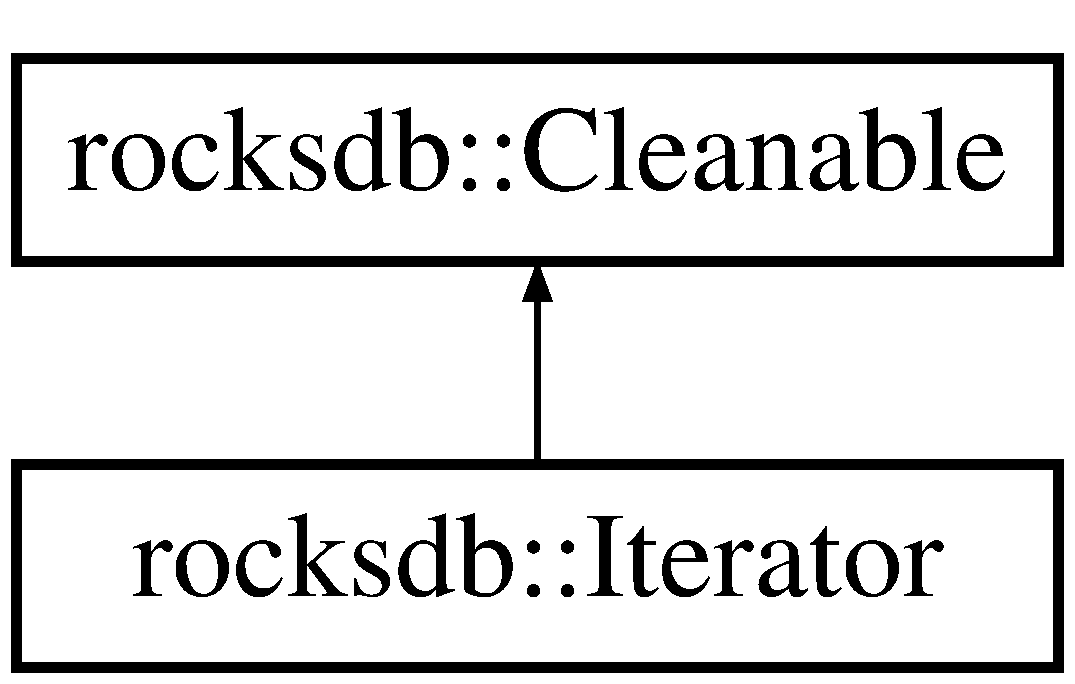
\includegraphics[height=2.000000cm]{classrocksdb_1_1Iterator}
\end{center}
\end{figure}
\subsection*{Public Member Functions}
\begin{DoxyCompactItemize}
\item 
virtual bool {\bfseries Valid} () const =0\hypertarget{classrocksdb_1_1Iterator_a866c8627787b3a768273ae4893f27f8f}{}\label{classrocksdb_1_1Iterator_a866c8627787b3a768273ae4893f27f8f}

\item 
virtual void {\bfseries Seek\+To\+First} ()=0\hypertarget{classrocksdb_1_1Iterator_a99d2e05c952cecb0f4a0fa60412bafc2}{}\label{classrocksdb_1_1Iterator_a99d2e05c952cecb0f4a0fa60412bafc2}

\item 
virtual void {\bfseries Seek\+To\+Last} ()=0\hypertarget{classrocksdb_1_1Iterator_a72603897beae5180e1785ee095ca43f4}{}\label{classrocksdb_1_1Iterator_a72603897beae5180e1785ee095ca43f4}

\item 
virtual void {\bfseries Seek} (const \hyperlink{classrocksdb_1_1Slice}{Slice} \&target)=0\hypertarget{classrocksdb_1_1Iterator_aeed06527f83bf2863595fc9514511d7d}{}\label{classrocksdb_1_1Iterator_aeed06527f83bf2863595fc9514511d7d}

\item 
virtual void {\bfseries Next} ()=0\hypertarget{classrocksdb_1_1Iterator_a06da095e0c88cc65ac23e4ec88d0a390}{}\label{classrocksdb_1_1Iterator_a06da095e0c88cc65ac23e4ec88d0a390}

\item 
virtual void {\bfseries Prev} ()=0\hypertarget{classrocksdb_1_1Iterator_acc6625d2209a48343c1ebce4c2528e23}{}\label{classrocksdb_1_1Iterator_acc6625d2209a48343c1ebce4c2528e23}

\item 
virtual \hyperlink{classrocksdb_1_1Slice}{Slice} {\bfseries key} () const =0\hypertarget{classrocksdb_1_1Iterator_a34cfd17f7b64652774de76cbc0e5b202}{}\label{classrocksdb_1_1Iterator_a34cfd17f7b64652774de76cbc0e5b202}

\item 
virtual \hyperlink{classrocksdb_1_1Slice}{Slice} {\bfseries value} () const =0\hypertarget{classrocksdb_1_1Iterator_a1a503134af26025486d5c640e49cdf54}{}\label{classrocksdb_1_1Iterator_a1a503134af26025486d5c640e49cdf54}

\item 
virtual \hyperlink{classrocksdb_1_1Status}{Status} {\bfseries status} () const =0\hypertarget{classrocksdb_1_1Iterator_a5435c832490b19d4c3aebf7c4877098d}{}\label{classrocksdb_1_1Iterator_a5435c832490b19d4c3aebf7c4877098d}

\item 
virtual \hyperlink{classrocksdb_1_1Status}{Status} {\bfseries Get\+Property} (std\+::string prop\+\_\+name, std\+::string $\ast$prop)\hypertarget{classrocksdb_1_1Iterator_a262a0e911087b145e95ac2a4603289f7}{}\label{classrocksdb_1_1Iterator_a262a0e911087b145e95ac2a4603289f7}

\end{DoxyCompactItemize}
\subsection*{Additional Inherited Members}


The documentation for this class was generated from the following file\+:\begin{DoxyCompactItemize}
\item 
Appserver/src/external/rocksdb/iterator.\+h\end{DoxyCompactItemize}

\hypertarget{structjson__token}{}\section{json\+\_\+token Struct Reference}
\label{structjson__token}\index{json\+\_\+token@{json\+\_\+token}}
\subsection*{Public Attributes}
\begin{DoxyCompactItemize}
\item 
const char $\ast$ {\bfseries ptr}\hypertarget{structjson__token_a2a93c938d0aa17cfbfa6a25f351c1004}{}\label{structjson__token_a2a93c938d0aa17cfbfa6a25f351c1004}

\item 
int {\bfseries len}\hypertarget{structjson__token_a62f334c0585bbc7b030dc0c2131dd127}{}\label{structjson__token_a62f334c0585bbc7b030dc0c2131dd127}

\item 
int {\bfseries num\+\_\+desc}\hypertarget{structjson__token_a88bdffe6c1b543a2cbfce4e6f4bf4814}{}\label{structjson__token_a88bdffe6c1b543a2cbfce4e6f4bf4814}

\item 
enum json\+\_\+type {\bfseries type}\hypertarget{structjson__token_a887277dca69b6162be38807ebfa568c9}{}\label{structjson__token_a887277dca69b6162be38807ebfa568c9}

\end{DoxyCompactItemize}


The documentation for this struct was generated from the following file\+:\begin{DoxyCompactItemize}
\item 
Appserver/src/external/mongoose/mongoose.\+h\end{DoxyCompactItemize}

\hypertarget{classJsonArray}{}\section{Json\+Array Class Reference}
\label{classJsonArray}\index{Json\+Array@{Json\+Array}}
Inheritance diagram for Json\+Array\+:\begin{figure}[H]
\begin{center}
\leavevmode
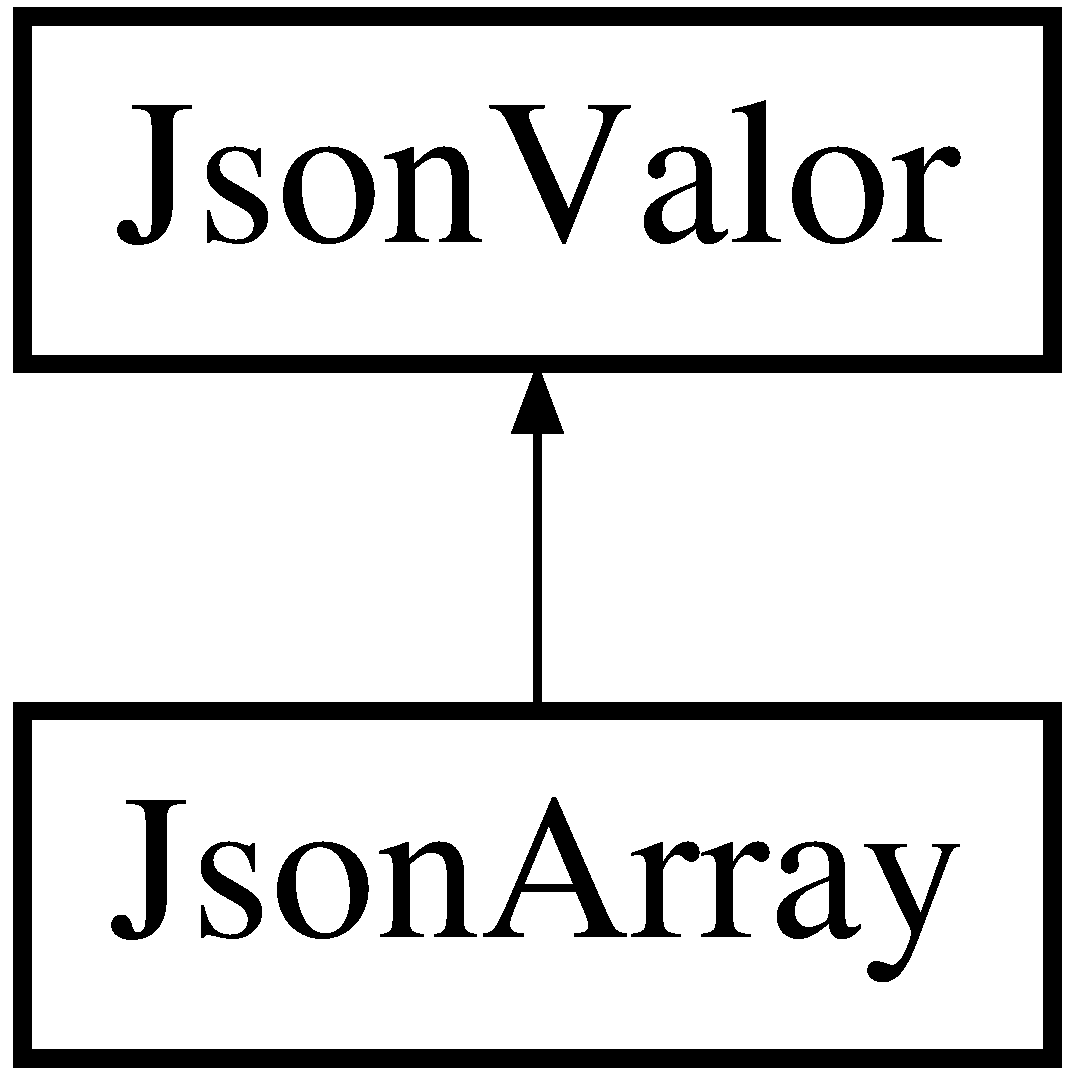
\includegraphics[height=2.000000cm]{classJsonArray}
\end{center}
\end{figure}
\subsection*{Public Member Functions}
\begin{DoxyCompactItemize}
\item 
{\bfseries Json\+Array} (string json\+Texto)\hypertarget{classJsonArray_a334673c1a44475daa1344da330e58380}{}\label{classJsonArray_a334673c1a44475daa1344da330e58380}

\item 
{\bfseries Json\+Array} (const \hyperlink{classJson_1_1Value}{Json\+::\+Value} \&json\+Valor)\hypertarget{classJsonArray_aafdd87de39f32d32b4776e3e859426be}{}\label{classJsonArray_aafdd87de39f32d32b4776e3e859426be}

\item 
bool {\bfseries operator$>$$>$} (string \&valor)\hypertarget{classJsonArray_a330f3f187aaa60083eb6dd0facfb3a30}{}\label{classJsonArray_a330f3f187aaa60083eb6dd0facfb3a30}

\item 
\hyperlink{classJsonValor}{Json\+Valor} {\bfseries operator\mbox{[}$\,$\mbox{]}} (int indice)\hypertarget{classJsonArray_a3b63e3235fcec3c372ee9edd0441febb}{}\label{classJsonArray_a3b63e3235fcec3c372ee9edd0441febb}

\item 
void {\bfseries agregar} (\hyperlink{classJsonValor}{Json\+Valor} \&valor)\hypertarget{classJsonArray_aa96dd1741e3abe071171056557f13649}{}\label{classJsonArray_aa96dd1741e3abe071171056557f13649}

\item 
void {\bfseries agregar} (string \&valor)\hypertarget{classJsonArray_a76b4ad22a247cf0e9c124918485eb526}{}\label{classJsonArray_a76b4ad22a247cf0e9c124918485eb526}

\item 
void {\bfseries agregar} (int \&valor)\hypertarget{classJsonArray_a92f3016e9bfc4d23feb8e85b1e99341b}{}\label{classJsonArray_a92f3016e9bfc4d23feb8e85b1e99341b}

\end{DoxyCompactItemize}
\subsection*{Additional Inherited Members}


The documentation for this class was generated from the following files\+:\begin{DoxyCompactItemize}
\item 
Appserver/src/servicios/Json\+Array.\+h\item 
Appserver/src/servicios/Json\+Array.\+cpp\end{DoxyCompactItemize}

\hypertarget{classrocksdb_1_1JSONDocument}{}\section{rocksdb\+:\+:J\+S\+O\+N\+Document Class Reference}
\label{classrocksdb_1_1JSONDocument}\index{rocksdb\+::\+J\+S\+O\+N\+Document@{rocksdb\+::\+J\+S\+O\+N\+Document}}
\subsection*{Public Types}
\begin{DoxyCompactItemize}
\item 
enum {\bfseries Type} \{ \\*
{\bfseries k\+Null}, 
{\bfseries k\+Array}, 
{\bfseries k\+Bool}, 
{\bfseries k\+Double}, 
\\*
{\bfseries k\+Int64}, 
{\bfseries k\+Object}, 
{\bfseries k\+String}
 \}\hypertarget{classrocksdb_1_1JSONDocument_a7a57b72ea9075589151ee9e8aff1ddf8}{}\label{classrocksdb_1_1JSONDocument_a7a57b72ea9075589151ee9e8aff1ddf8}

\end{DoxyCompactItemize}
\subsection*{Public Member Functions}
\begin{DoxyCompactItemize}
\item 
{\bfseries J\+S\+O\+N\+Document} (bool b)\hypertarget{classrocksdb_1_1JSONDocument_acb472e7939a3beac180ed7057f91ac4a}{}\label{classrocksdb_1_1JSONDocument_acb472e7939a3beac180ed7057f91ac4a}

\item 
{\bfseries J\+S\+O\+N\+Document} (double d)\hypertarget{classrocksdb_1_1JSONDocument_a34b25c53329b82f45eb32a675985b039}{}\label{classrocksdb_1_1JSONDocument_a34b25c53329b82f45eb32a675985b039}

\item 
{\bfseries J\+S\+O\+N\+Document} (int8\+\_\+t i)\hypertarget{classrocksdb_1_1JSONDocument_a5348870ce6c0f2e9f5c805c57016a131}{}\label{classrocksdb_1_1JSONDocument_a5348870ce6c0f2e9f5c805c57016a131}

\item 
{\bfseries J\+S\+O\+N\+Document} (int16\+\_\+t i)\hypertarget{classrocksdb_1_1JSONDocument_a992cb3d9c8e4489a471a28f394d54416}{}\label{classrocksdb_1_1JSONDocument_a992cb3d9c8e4489a471a28f394d54416}

\item 
{\bfseries J\+S\+O\+N\+Document} (int32\+\_\+t i)\hypertarget{classrocksdb_1_1JSONDocument_ab122a61ef505fd0b384cc61b0cd5cc8a}{}\label{classrocksdb_1_1JSONDocument_ab122a61ef505fd0b384cc61b0cd5cc8a}

\item 
{\bfseries J\+S\+O\+N\+Document} (int64\+\_\+t i)\hypertarget{classrocksdb_1_1JSONDocument_a31c519799de83d32cb013a0a21a02b04}{}\label{classrocksdb_1_1JSONDocument_a31c519799de83d32cb013a0a21a02b04}

\item 
{\bfseries J\+S\+O\+N\+Document} (const std\+::string \&s)\hypertarget{classrocksdb_1_1JSONDocument_aadc4879774f7156d40680750878ebead}{}\label{classrocksdb_1_1JSONDocument_aadc4879774f7156d40680750878ebead}

\item 
{\bfseries J\+S\+O\+N\+Document} (const char $\ast$s)\hypertarget{classrocksdb_1_1JSONDocument_a5b3dea6b5a1deabce9198213d4735dea}{}\label{classrocksdb_1_1JSONDocument_a5b3dea6b5a1deabce9198213d4735dea}

\item 
{\bfseries J\+S\+O\+N\+Document} (Type \+\_\+type)\hypertarget{classrocksdb_1_1JSONDocument_a7734a18e81252e0e197a4dbf7cdb75ec}{}\label{classrocksdb_1_1JSONDocument_a7734a18e81252e0e197a4dbf7cdb75ec}

\item 
{\bfseries J\+S\+O\+N\+Document} (const \hyperlink{classrocksdb_1_1JSONDocument}{J\+S\+O\+N\+Document} \&json\+\_\+document)\hypertarget{classrocksdb_1_1JSONDocument_ac054de19e7260a00f7bb7f83daf502a2}{}\label{classrocksdb_1_1JSONDocument_ac054de19e7260a00f7bb7f83daf502a2}

\item 
{\bfseries J\+S\+O\+N\+Document} (\hyperlink{classrocksdb_1_1JSONDocument}{J\+S\+O\+N\+Document} \&\&json\+\_\+document)\hypertarget{classrocksdb_1_1JSONDocument_ad3b691c15e9e66547c1d6598b72fbe5a}{}\label{classrocksdb_1_1JSONDocument_ad3b691c15e9e66547c1d6598b72fbe5a}

\item 
Type {\bfseries type} () const\hypertarget{classrocksdb_1_1JSONDocument_ae24738c5b23619b63ae7e9c923629ca9}{}\label{classrocksdb_1_1JSONDocument_ae24738c5b23619b63ae7e9c923629ca9}

\item 
bool {\bfseries Contains} (const std\+::string \&key) const\hypertarget{classrocksdb_1_1JSONDocument_a7ca62d131a53c40c87a354dc61d3e2f2}{}\label{classrocksdb_1_1JSONDocument_a7ca62d131a53c40c87a354dc61d3e2f2}

\item 
\hyperlink{classrocksdb_1_1JSONDocument}{J\+S\+O\+N\+Document} {\bfseries operator\mbox{[}$\,$\mbox{]}} (const std\+::string \&key) const\hypertarget{classrocksdb_1_1JSONDocument_a515dc269b2fc74c5baf0619f946d18b0}{}\label{classrocksdb_1_1JSONDocument_a515dc269b2fc74c5baf0619f946d18b0}

\item 
size\+\_\+t {\bfseries Count} () const\hypertarget{classrocksdb_1_1JSONDocument_a2e66abdc3d34d0816428c69b05de8a5d}{}\label{classrocksdb_1_1JSONDocument_a2e66abdc3d34d0816428c69b05de8a5d}

\item 
\hyperlink{classrocksdb_1_1JSONDocument}{J\+S\+O\+N\+Document} {\bfseries operator\mbox{[}$\,$\mbox{]}} (size\+\_\+t i) const\hypertarget{classrocksdb_1_1JSONDocument_a14b3a9783230c00537405a9acd7ff589}{}\label{classrocksdb_1_1JSONDocument_a14b3a9783230c00537405a9acd7ff589}

\item 
\hyperlink{classrocksdb_1_1JSONDocument}{J\+S\+O\+N\+Document} \& {\bfseries operator=} (\hyperlink{classrocksdb_1_1JSONDocument}{J\+S\+O\+N\+Document} json\+Document)\hypertarget{classrocksdb_1_1JSONDocument_a31b25cb70dcf002311e2289a3a7f03a6}{}\label{classrocksdb_1_1JSONDocument_a31b25cb70dcf002311e2289a3a7f03a6}

\item 
bool {\bfseries Is\+Null} () const\hypertarget{classrocksdb_1_1JSONDocument_ab4cee9806fa563e5a3de20d936875836}{}\label{classrocksdb_1_1JSONDocument_ab4cee9806fa563e5a3de20d936875836}

\item 
bool {\bfseries Is\+Array} () const\hypertarget{classrocksdb_1_1JSONDocument_a20544f3bd7ab50af8ef30025d2cf17f7}{}\label{classrocksdb_1_1JSONDocument_a20544f3bd7ab50af8ef30025d2cf17f7}

\item 
bool {\bfseries Is\+Bool} () const\hypertarget{classrocksdb_1_1JSONDocument_a53643c5b29b28da4b173d5b4cb7245db}{}\label{classrocksdb_1_1JSONDocument_a53643c5b29b28da4b173d5b4cb7245db}

\item 
bool {\bfseries Is\+Double} () const\hypertarget{classrocksdb_1_1JSONDocument_af3c036924c68cc1a699efa3a22b17b42}{}\label{classrocksdb_1_1JSONDocument_af3c036924c68cc1a699efa3a22b17b42}

\item 
bool {\bfseries Is\+Int64} () const\hypertarget{classrocksdb_1_1JSONDocument_a66a4efa29267abc77ed9778434651d95}{}\label{classrocksdb_1_1JSONDocument_a66a4efa29267abc77ed9778434651d95}

\item 
bool {\bfseries Is\+Object} () const\hypertarget{classrocksdb_1_1JSONDocument_a5e4e43bbf660cde813101f877744e8be}{}\label{classrocksdb_1_1JSONDocument_a5e4e43bbf660cde813101f877744e8be}

\item 
bool {\bfseries Is\+String} () const\hypertarget{classrocksdb_1_1JSONDocument_a51cba56fc4c6d8e5fd7609d6c2483036}{}\label{classrocksdb_1_1JSONDocument_a51cba56fc4c6d8e5fd7609d6c2483036}

\item 
bool {\bfseries Get\+Bool} () const\hypertarget{classrocksdb_1_1JSONDocument_afea7227a4530a605b87eec8ef1305129}{}\label{classrocksdb_1_1JSONDocument_afea7227a4530a605b87eec8ef1305129}

\item 
double {\bfseries Get\+Double} () const\hypertarget{classrocksdb_1_1JSONDocument_ac241778c6e274181cb0d7e4e7000bd55}{}\label{classrocksdb_1_1JSONDocument_ac241778c6e274181cb0d7e4e7000bd55}

\item 
int64\+\_\+t {\bfseries Get\+Int64} () const\hypertarget{classrocksdb_1_1JSONDocument_ab1bf996631710cf7fe3e996c50747b72}{}\label{classrocksdb_1_1JSONDocument_ab1bf996631710cf7fe3e996c50747b72}

\item 
std\+::string {\bfseries Get\+String} () const\hypertarget{classrocksdb_1_1JSONDocument_a864751667501f13941f4268a38f901ce}{}\label{classrocksdb_1_1JSONDocument_a864751667501f13941f4268a38f901ce}

\item 
bool {\bfseries operator==} (const \hyperlink{classrocksdb_1_1JSONDocument}{J\+S\+O\+N\+Document} \&rhs) const\hypertarget{classrocksdb_1_1JSONDocument_a0d7c520c34f92a381ad6585854de755e}{}\label{classrocksdb_1_1JSONDocument_a0d7c520c34f92a381ad6585854de755e}

\item 
bool {\bfseries operator!=} (const \hyperlink{classrocksdb_1_1JSONDocument}{J\+S\+O\+N\+Document} \&rhs) const\hypertarget{classrocksdb_1_1JSONDocument_a9ad0f6d65c09766b5e3c8a55c069fcfd}{}\label{classrocksdb_1_1JSONDocument_a9ad0f6d65c09766b5e3c8a55c069fcfd}

\item 
\hyperlink{classrocksdb_1_1JSONDocument}{J\+S\+O\+N\+Document} {\bfseries Copy} () const\hypertarget{classrocksdb_1_1JSONDocument_abd8eb5a045c72159429d9a8c4fae3ec4}{}\label{classrocksdb_1_1JSONDocument_abd8eb5a045c72159429d9a8c4fae3ec4}

\item 
bool {\bfseries Is\+Owner} () const\hypertarget{classrocksdb_1_1JSONDocument_a5018105d97e08df2ea66f7623237b217}{}\label{classrocksdb_1_1JSONDocument_a5018105d97e08df2ea66f7623237b217}

\item 
std\+::string {\bfseries Debug\+String} () const\hypertarget{classrocksdb_1_1JSONDocument_a4be12cd91ce9b582b701548ad97abbd3}{}\label{classrocksdb_1_1JSONDocument_a4be12cd91ce9b582b701548ad97abbd3}

\item 
Items\+Iterator\+Generator {\bfseries Items} () const\hypertarget{classrocksdb_1_1JSONDocument_af83edc7279e5abe6986001d3e9947da8}{}\label{classrocksdb_1_1JSONDocument_af83edc7279e5abe6986001d3e9947da8}

\item 
void {\bfseries Serialize} (std\+::string $\ast$dst) const\hypertarget{classrocksdb_1_1JSONDocument_a244aba5520db6bd7b7102d3e13c78336}{}\label{classrocksdb_1_1JSONDocument_a244aba5520db6bd7b7102d3e13c78336}

\end{DoxyCompactItemize}
\subsection*{Static Public Member Functions}
\begin{DoxyCompactItemize}
\item 
static \hyperlink{classrocksdb_1_1JSONDocument}{J\+S\+O\+N\+Document} $\ast$ {\bfseries Parse\+J\+S\+ON} (const char $\ast$json)\hypertarget{classrocksdb_1_1JSONDocument_a25424fd51385c0c795bd9d95d53b85bc}{}\label{classrocksdb_1_1JSONDocument_a25424fd51385c0c795bd9d95d53b85bc}

\item 
static \hyperlink{classrocksdb_1_1JSONDocument}{J\+S\+O\+N\+Document} $\ast$ {\bfseries Deserialize} (const \hyperlink{classrocksdb_1_1Slice}{Slice} \&src)\hypertarget{classrocksdb_1_1JSONDocument_af16c6f77dc3c402fd5fd4fc4be1c6264}{}\label{classrocksdb_1_1JSONDocument_af16c6f77dc3c402fd5fd4fc4be1c6264}

\end{DoxyCompactItemize}
\subsection*{Friends}
\begin{DoxyCompactItemize}
\item 
class {\bfseries J\+S\+O\+N\+Document\+Builder}\hypertarget{classrocksdb_1_1JSONDocument_aca5ff666ab7c2a88cd39d1827e970a36}{}\label{classrocksdb_1_1JSONDocument_aca5ff666ab7c2a88cd39d1827e970a36}

\end{DoxyCompactItemize}


The documentation for this class was generated from the following file\+:\begin{DoxyCompactItemize}
\item 
Appserver/src/external/rocksdb/utilities/json\+\_\+document.\+h\end{DoxyCompactItemize}

\hypertarget{classrocksdb_1_1JSONDocumentBuilder}{}\section{rocksdb\+:\+:J\+S\+O\+N\+Document\+Builder Class Reference}
\label{classrocksdb_1_1JSONDocumentBuilder}\index{rocksdb\+::\+J\+S\+O\+N\+Document\+Builder@{rocksdb\+::\+J\+S\+O\+N\+Document\+Builder}}
\subsection*{Public Member Functions}
\begin{DoxyCompactItemize}
\item 
{\bfseries J\+S\+O\+N\+Document\+Builder} (fbson\+::\+Fbson\+Out\+Stream $\ast$out)\hypertarget{classrocksdb_1_1JSONDocumentBuilder_ad576a62168d75b9b02d34c7b841de458}{}\label{classrocksdb_1_1JSONDocumentBuilder_ad576a62168d75b9b02d34c7b841de458}

\item 
void {\bfseries Reset} ()\hypertarget{classrocksdb_1_1JSONDocumentBuilder_a8b7f8d5c309bca9fdba2963fe7101747}{}\label{classrocksdb_1_1JSONDocumentBuilder_a8b7f8d5c309bca9fdba2963fe7101747}

\item 
bool {\bfseries Write\+Start\+Array} ()\hypertarget{classrocksdb_1_1JSONDocumentBuilder_a6c1e590614f2e8d6f75e45600aa8a182}{}\label{classrocksdb_1_1JSONDocumentBuilder_a6c1e590614f2e8d6f75e45600aa8a182}

\item 
bool {\bfseries Write\+End\+Array} ()\hypertarget{classrocksdb_1_1JSONDocumentBuilder_af9e0e0a04d0531a27e2c65ae79cf6c4d}{}\label{classrocksdb_1_1JSONDocumentBuilder_af9e0e0a04d0531a27e2c65ae79cf6c4d}

\item 
bool {\bfseries Write\+Start\+Object} ()\hypertarget{classrocksdb_1_1JSONDocumentBuilder_aa1bbac7729f273f0f83a7f5fc5dc90ab}{}\label{classrocksdb_1_1JSONDocumentBuilder_aa1bbac7729f273f0f83a7f5fc5dc90ab}

\item 
bool {\bfseries Write\+End\+Object} ()\hypertarget{classrocksdb_1_1JSONDocumentBuilder_a9b1ad02c35affee1ee732e39d50bade9}{}\label{classrocksdb_1_1JSONDocumentBuilder_a9b1ad02c35affee1ee732e39d50bade9}

\item 
bool {\bfseries Write\+Key\+Value} (const std\+::string \&key, const \hyperlink{classrocksdb_1_1JSONDocument}{J\+S\+O\+N\+Document} \&value)\hypertarget{classrocksdb_1_1JSONDocumentBuilder_a83b321329e48e49b070f95c851839bbf}{}\label{classrocksdb_1_1JSONDocumentBuilder_a83b321329e48e49b070f95c851839bbf}

\item 
bool {\bfseries Write\+J\+S\+O\+N\+Document} (const \hyperlink{classrocksdb_1_1JSONDocument}{J\+S\+O\+N\+Document} \&value)\hypertarget{classrocksdb_1_1JSONDocumentBuilder_a41e74919ea2157aeb387bbeb8e685584}{}\label{classrocksdb_1_1JSONDocumentBuilder_a41e74919ea2157aeb387bbeb8e685584}

\item 
\hyperlink{classrocksdb_1_1JSONDocument}{J\+S\+O\+N\+Document} {\bfseries Get\+J\+S\+O\+N\+Document} ()\hypertarget{classrocksdb_1_1JSONDocumentBuilder_ab3c16986e0eea459995c0d6aa96911b3}{}\label{classrocksdb_1_1JSONDocumentBuilder_ab3c16986e0eea459995c0d6aa96911b3}

\end{DoxyCompactItemize}


The documentation for this class was generated from the following file\+:\begin{DoxyCompactItemize}
\item 
Appserver/src/external/rocksdb/utilities/json\+\_\+document.\+h\end{DoxyCompactItemize}

\hypertarget{classJsonObject}{}\section{Json\+Object Class Reference}
\label{classJsonObject}\index{Json\+Object@{Json\+Object}}
Inheritance diagram for Json\+Object\+:\begin{figure}[H]
\begin{center}
\leavevmode
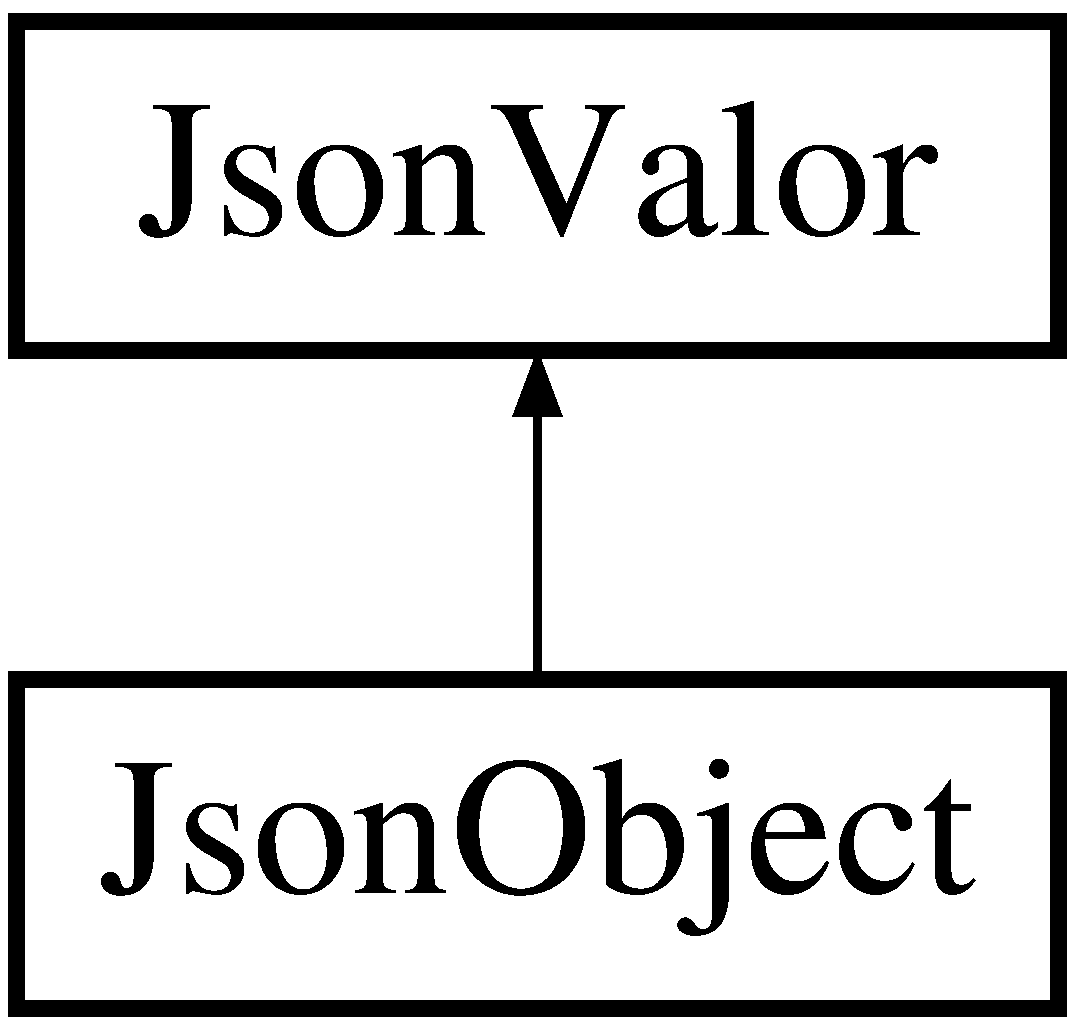
\includegraphics[height=2.000000cm]{classJsonObject}
\end{center}
\end{figure}
\subsection*{Public Member Functions}
\begin{DoxyCompactItemize}
\item 
{\bfseries Json\+Object} (string json\+Texto)\hypertarget{classJsonObject_a37c52e97d2b4187171f5226bb11ddbf6}{}\label{classJsonObject_a37c52e97d2b4187171f5226bb11ddbf6}

\item 
{\bfseries Json\+Object} (const \hyperlink{classJson_1_1Value}{Json\+::\+Value} \&json\+Valor)\hypertarget{classJsonObject_abe2ab40281a208a16983a8c9e950a4a7}{}\label{classJsonObject_abe2ab40281a208a16983a8c9e950a4a7}

\item 
\hyperlink{classJsonValor}{Json\+Valor} {\bfseries operator\mbox{[}$\,$\mbox{]}} (string clave)\hypertarget{classJsonObject_a8f37b0bd7a2de2c0c2e0ee5a43d794b3}{}\label{classJsonObject_a8f37b0bd7a2de2c0c2e0ee5a43d794b3}

\item 
\hyperlink{classJsonObject}{Json\+Object} {\bfseries get\+Json\+Object} (string clave)\hypertarget{classJsonObject_a268075faf3d74db5ffd26d6aa13611fd}{}\label{classJsonObject_a268075faf3d74db5ffd26d6aa13611fd}

\item 
\hyperlink{classJsonArray}{Json\+Array} {\bfseries get\+Json\+Array} (string clave)\hypertarget{classJsonObject_a9a52a2f313f93bf923adfadff451831e}{}\label{classJsonObject_a9a52a2f313f93bf923adfadff451831e}

\item 
int {\bfseries get\+Int} (string clave)\hypertarget{classJsonObject_abfcf9120de35a4977c278e5b9136b584}{}\label{classJsonObject_abfcf9120de35a4977c278e5b9136b584}

\item 
string {\bfseries get\+String} (string clave)\hypertarget{classJsonObject_aaacd804f6b16d215c8b942fb02e22a7e}{}\label{classJsonObject_aaacd804f6b16d215c8b942fb02e22a7e}

\item 
void {\bfseries agregar\+Clave\+Valor} (string clave, string valor)\hypertarget{classJsonObject_a6e4d553543a3dbfd75d09c1ab449b025}{}\label{classJsonObject_a6e4d553543a3dbfd75d09c1ab449b025}

\item 
void {\bfseries agregar\+Clave\+Valor} (string clave, int valor)\hypertarget{classJsonObject_ab77f4672fdc67815e5b89bb83c6bc937}{}\label{classJsonObject_ab77f4672fdc67815e5b89bb83c6bc937}

\item 
void {\bfseries agregar\+Clave\+Valor} (string clave, \hyperlink{classJsonValor}{Json\+Valor} \&valor)\hypertarget{classJsonObject_a47d0887639448348e4c750f1cbcea254}{}\label{classJsonObject_a47d0887639448348e4c750f1cbcea254}

\end{DoxyCompactItemize}
\subsection*{Additional Inherited Members}


The documentation for this class was generated from the following files\+:\begin{DoxyCompactItemize}
\item 
Appserver/src/servicios/Json\+Object.\+h\item 
Appserver/src/servicios/Json\+Object.\+cpp\end{DoxyCompactItemize}

\hypertarget{classJsonValor}{}\section{Json\+Valor Class Reference}
\label{classJsonValor}\index{Json\+Valor@{Json\+Valor}}
Inheritance diagram for Json\+Valor\+:\begin{figure}[H]
\begin{center}
\leavevmode
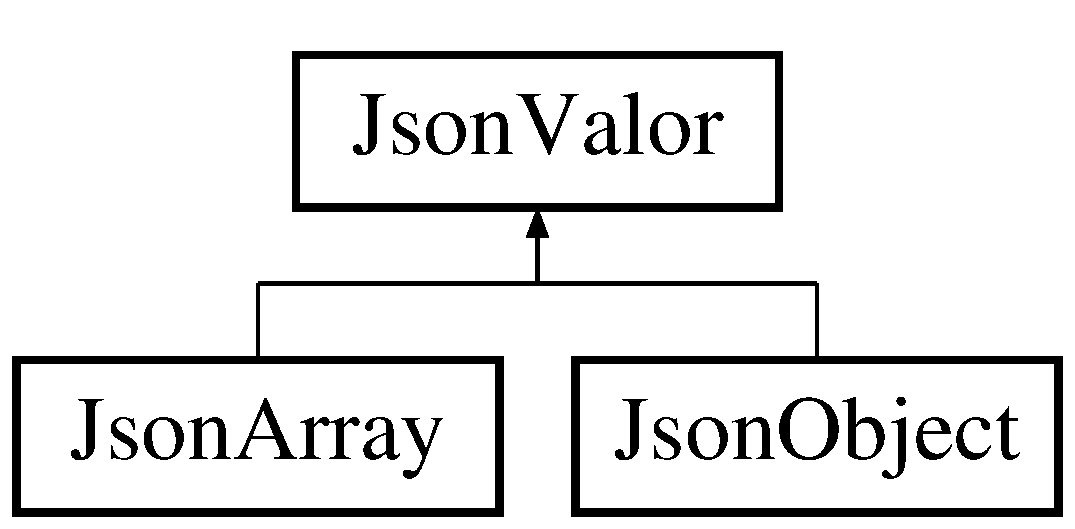
\includegraphics[height=2.000000cm]{classJsonValor}
\end{center}
\end{figure}
\subsection*{Public Member Functions}
\begin{DoxyCompactItemize}
\item 
{\bfseries Json\+Valor} (string json\+Texto)\hypertarget{classJsonValor_a7f772d055e8b997bcbb04c0d6ead9537}{}\label{classJsonValor_a7f772d055e8b997bcbb04c0d6ead9537}

\item 
{\bfseries Json\+Valor} (const \hyperlink{classJson_1_1Value}{Json\+::\+Value} \&json\+Valor)\hypertarget{classJsonValor_a4a28b4470b6efdcf08b9551fa713e02f}{}\label{classJsonValor_a4a28b4470b6efdcf08b9551fa713e02f}

\item 
\hyperlink{classJson_1_1Value}{Json\+::\+Value} \& {\bfseries get\+Json\+Value} ()\hypertarget{classJsonValor_aed661fdbe7cdd4cae14165a3c9ea8965}{}\label{classJsonValor_aed661fdbe7cdd4cae14165a3c9ea8965}

\item 
int {\bfseries size} ()\hypertarget{classJsonValor_a3743ad009175d884263a51ec659638f9}{}\label{classJsonValor_a3743ad009175d884263a51ec659638f9}

\item 
string {\bfseries to\+String} ()\hypertarget{classJsonValor_adcea7ce81e014bf14b67983c1bea3282}{}\label{classJsonValor_adcea7ce81e014bf14b67983c1bea3282}

\end{DoxyCompactItemize}
\subsection*{Protected Attributes}
\begin{DoxyCompactItemize}
\item 
\hyperlink{classJson_1_1Value}{Json\+::\+Value} {\bfseries json\+Valor}\hypertarget{classJsonValor_a9dc5f72fb7f56a1d6182f16e7ec8e696}{}\label{classJsonValor_a9dc5f72fb7f56a1d6182f16e7ec8e696}

\end{DoxyCompactItemize}


The documentation for this class was generated from the following files\+:\begin{DoxyCompactItemize}
\item 
Appserver/src/servicios/Json\+Valor.\+h\item 
Appserver/src/servicios/Json\+Valor.\+cpp\end{DoxyCompactItemize}

\hypertarget{classrocksdb_1_1MemTableRep_1_1KeyComparator}{}\section{rocksdb\+:\+:Mem\+Table\+Rep\+:\+:Key\+Comparator Class Reference}
\label{classrocksdb_1_1MemTableRep_1_1KeyComparator}\index{rocksdb\+::\+Mem\+Table\+Rep\+::\+Key\+Comparator@{rocksdb\+::\+Mem\+Table\+Rep\+::\+Key\+Comparator}}
\subsection*{Public Member Functions}
\begin{DoxyCompactItemize}
\item 
virtual int {\bfseries operator()} (const char $\ast$prefix\+\_\+len\+\_\+key1, const char $\ast$prefix\+\_\+len\+\_\+key2) const =0\hypertarget{classrocksdb_1_1MemTableRep_1_1KeyComparator_a7d9ddc98e3bc44efbb77197428f5ae5a}{}\label{classrocksdb_1_1MemTableRep_1_1KeyComparator_a7d9ddc98e3bc44efbb77197428f5ae5a}

\item 
virtual int {\bfseries operator()} (const char $\ast$prefix\+\_\+len\+\_\+key, const \hyperlink{classrocksdb_1_1Slice}{Slice} \&key) const =0\hypertarget{classrocksdb_1_1MemTableRep_1_1KeyComparator_ab17adac38a1b69c57832801223a4efa2}{}\label{classrocksdb_1_1MemTableRep_1_1KeyComparator_ab17adac38a1b69c57832801223a4efa2}

\end{DoxyCompactItemize}


The documentation for this class was generated from the following file\+:\begin{DoxyCompactItemize}
\item 
Appserver/src/external/rocksdb/memtablerep.\+h\end{DoxyCompactItemize}

\hypertarget{structrocksdb_1_1LDBOptions}{}\section{rocksdb\+:\+:L\+D\+B\+Options Struct Reference}
\label{structrocksdb_1_1LDBOptions}\index{rocksdb\+::\+L\+D\+B\+Options@{rocksdb\+::\+L\+D\+B\+Options}}
\subsection*{Public Attributes}
\begin{DoxyCompactItemize}
\item 
std\+::shared\+\_\+ptr$<$ \hyperlink{classrocksdb_1_1SliceFormatter}{Slice\+Formatter} $>$ {\bfseries key\+\_\+formatter}\hypertarget{structrocksdb_1_1LDBOptions_afc3f242e28b1f1980c568e5c5374e4f0}{}\label{structrocksdb_1_1LDBOptions_afc3f242e28b1f1980c568e5c5374e4f0}

\end{DoxyCompactItemize}


The documentation for this struct was generated from the following file\+:\begin{DoxyCompactItemize}
\item 
Appserver/src/external/rocksdb/ldb\+\_\+tool.\+h\end{DoxyCompactItemize}

\hypertarget{classrocksdb_1_1LDBTool}{}\section{rocksdb\+:\+:L\+D\+B\+Tool Class Reference}
\label{classrocksdb_1_1LDBTool}\index{rocksdb\+::\+L\+D\+B\+Tool@{rocksdb\+::\+L\+D\+B\+Tool}}
\subsection*{Public Member Functions}
\begin{DoxyCompactItemize}
\item 
void {\bfseries Run} (int argc, char $\ast$$\ast$argv, \hyperlink{structrocksdb_1_1Options}{Options} db\+\_\+options=\hyperlink{structrocksdb_1_1Options}{Options}(), const \hyperlink{structrocksdb_1_1LDBOptions}{L\+D\+B\+Options} \&ldb\+\_\+options=\hyperlink{structrocksdb_1_1LDBOptions}{L\+D\+B\+Options}(), const std\+::vector$<$ \hyperlink{structrocksdb_1_1ColumnFamilyDescriptor}{Column\+Family\+Descriptor} $>$ $\ast$column\+\_\+families=nullptr)\hypertarget{classrocksdb_1_1LDBTool_ab9a6f4487ad6f89a483cf7f0aa70118c}{}\label{classrocksdb_1_1LDBTool_ab9a6f4487ad6f89a483cf7f0aa70118c}

\end{DoxyCompactItemize}


The documentation for this class was generated from the following file\+:\begin{DoxyCompactItemize}
\item 
Appserver/src/external/rocksdb/ldb\+\_\+tool.\+h\end{DoxyCompactItemize}

\hypertarget{structrocksdb_1_1LevelDBOptions}{}\section{rocksdb\+:\+:Level\+D\+B\+Options Struct Reference}
\label{structrocksdb_1_1LevelDBOptions}\index{rocksdb\+::\+Level\+D\+B\+Options@{rocksdb\+::\+Level\+D\+B\+Options}}
\subsection*{Public Attributes}
\begin{DoxyCompactItemize}
\item 
const \hyperlink{classrocksdb_1_1Comparator}{Comparator} $\ast$ {\bfseries comparator}\hypertarget{structrocksdb_1_1LevelDBOptions_ab3390627c2c3f9af0f9edddef698a555}{}\label{structrocksdb_1_1LevelDBOptions_ab3390627c2c3f9af0f9edddef698a555}

\item 
bool {\bfseries create\+\_\+if\+\_\+missing}\hypertarget{structrocksdb_1_1LevelDBOptions_a144bbb9a60d576073e674f26c41be7fa}{}\label{structrocksdb_1_1LevelDBOptions_a144bbb9a60d576073e674f26c41be7fa}

\item 
bool {\bfseries error\+\_\+if\+\_\+exists}\hypertarget{structrocksdb_1_1LevelDBOptions_a223d40836644e508965e0e991b8d95ca}{}\label{structrocksdb_1_1LevelDBOptions_a223d40836644e508965e0e991b8d95ca}

\item 
bool {\bfseries paranoid\+\_\+checks}\hypertarget{structrocksdb_1_1LevelDBOptions_a9e63a2c4d47896d1385559ba32200cad}{}\label{structrocksdb_1_1LevelDBOptions_a9e63a2c4d47896d1385559ba32200cad}

\item 
\hyperlink{classrocksdb_1_1Env}{Env} $\ast$ {\bfseries env}\hypertarget{structrocksdb_1_1LevelDBOptions_ab9822177833d9da4f88482835dcf19d2}{}\label{structrocksdb_1_1LevelDBOptions_ab9822177833d9da4f88482835dcf19d2}

\item 
\hyperlink{classrocksdb_1_1Logger}{Logger} $\ast$ {\bfseries info\+\_\+log}\hypertarget{structrocksdb_1_1LevelDBOptions_a56e3ee9faa9d2b2745cabcdcd9e242f7}{}\label{structrocksdb_1_1LevelDBOptions_a56e3ee9faa9d2b2745cabcdcd9e242f7}

\item 
size\+\_\+t {\bfseries write\+\_\+buffer\+\_\+size}\hypertarget{structrocksdb_1_1LevelDBOptions_a7691054488c72ecb34c734e861ea3a97}{}\label{structrocksdb_1_1LevelDBOptions_a7691054488c72ecb34c734e861ea3a97}

\item 
int {\bfseries max\+\_\+open\+\_\+files}\hypertarget{structrocksdb_1_1LevelDBOptions_aef717385b3d0e2868e09c755de31575a}{}\label{structrocksdb_1_1LevelDBOptions_aef717385b3d0e2868e09c755de31575a}

\item 
\hyperlink{classrocksdb_1_1Cache}{Cache} $\ast$ {\bfseries block\+\_\+cache}\hypertarget{structrocksdb_1_1LevelDBOptions_a535719d0da82c8c57724a5f52de9b2d5}{}\label{structrocksdb_1_1LevelDBOptions_a535719d0da82c8c57724a5f52de9b2d5}

\item 
size\+\_\+t {\bfseries block\+\_\+size}\hypertarget{structrocksdb_1_1LevelDBOptions_a086a3829758119178fe32358259cfd6f}{}\label{structrocksdb_1_1LevelDBOptions_a086a3829758119178fe32358259cfd6f}

\item 
int {\bfseries block\+\_\+restart\+\_\+interval}\hypertarget{structrocksdb_1_1LevelDBOptions_a906eb3051388f6e530e0868af22e065d}{}\label{structrocksdb_1_1LevelDBOptions_a906eb3051388f6e530e0868af22e065d}

\item 
Compression\+Type {\bfseries compression}\hypertarget{structrocksdb_1_1LevelDBOptions_adc67c994a2b43000064d7365dddef026}{}\label{structrocksdb_1_1LevelDBOptions_adc67c994a2b43000064d7365dddef026}

\item 
const \hyperlink{classrocksdb_1_1FilterPolicy}{Filter\+Policy} $\ast$ {\bfseries filter\+\_\+policy}\hypertarget{structrocksdb_1_1LevelDBOptions_ab213c2c0f4827ae42d403de95fe8c6b3}{}\label{structrocksdb_1_1LevelDBOptions_ab213c2c0f4827ae42d403de95fe8c6b3}

\end{DoxyCompactItemize}


The documentation for this struct was generated from the following file\+:\begin{DoxyCompactItemize}
\item 
Appserver/src/external/rocksdb/utilities/leveldb\+\_\+options.\+h\end{DoxyCompactItemize}

\hypertarget{structrocksdb_1_1LevelMetaData}{}\section{rocksdb\+:\+:Level\+Meta\+Data Struct Reference}
\label{structrocksdb_1_1LevelMetaData}\index{rocksdb\+::\+Level\+Meta\+Data@{rocksdb\+::\+Level\+Meta\+Data}}
\subsection*{Public Member Functions}
\begin{DoxyCompactItemize}
\item 
{\bfseries Level\+Meta\+Data} (int \+\_\+level, uint64\+\_\+t \+\_\+size, const std\+::vector$<$ \hyperlink{structrocksdb_1_1SstFileMetaData}{Sst\+File\+Meta\+Data} $>$ \&\&\+\_\+files)\hypertarget{structrocksdb_1_1LevelMetaData_aa76b1ae21d24c6ecdc941809a2486d38}{}\label{structrocksdb_1_1LevelMetaData_aa76b1ae21d24c6ecdc941809a2486d38}

\end{DoxyCompactItemize}
\subsection*{Public Attributes}
\begin{DoxyCompactItemize}
\item 
const int {\bfseries level}\hypertarget{structrocksdb_1_1LevelMetaData_a7e937239c43763851507c13c79275a63}{}\label{structrocksdb_1_1LevelMetaData_a7e937239c43763851507c13c79275a63}

\item 
const uint64\+\_\+t {\bfseries size}\hypertarget{structrocksdb_1_1LevelMetaData_a79efd06d2b73900b508e248fe0633e26}{}\label{structrocksdb_1_1LevelMetaData_a79efd06d2b73900b508e248fe0633e26}

\item 
const std\+::vector$<$ \hyperlink{structrocksdb_1_1SstFileMetaData}{Sst\+File\+Meta\+Data} $>$ {\bfseries files}\hypertarget{structrocksdb_1_1LevelMetaData_a16a5833f8818bc0868709be0ada41381}{}\label{structrocksdb_1_1LevelMetaData_a16a5833f8818bc0868709be0ada41381}

\end{DoxyCompactItemize}


The documentation for this struct was generated from the following file\+:\begin{DoxyCompactItemize}
\item 
Appserver/src/external/rocksdb/metadata.\+h\end{DoxyCompactItemize}

\hypertarget{classListadoDeIntereses}{}\section{Listado\+De\+Intereses Class Reference}
\label{classListadoDeIntereses}\index{Listado\+De\+Intereses@{Listado\+De\+Intereses}}
\subsection*{Public Member Functions}
\begin{DoxyCompactItemize}
\item 
void {\bfseries agregar\+Intereses} (string json\+Listado\+Intereses)\hypertarget{classListadoDeIntereses_a148967d35fc5714b1a8158dc60cd80a8}{}\label{classListadoDeIntereses_a148967d35fc5714b1a8158dc60cd80a8}

\item 
bool {\bfseries tiene\+Interes} (\hyperlink{classInteres}{Interes} \&interes)\hypertarget{classListadoDeIntereses_aa7178e2b423992b423f1d1196ea819dc}{}\label{classListadoDeIntereses_aa7178e2b423992b423f1d1196ea819dc}

\item 
int {\bfseries size} ()\hypertarget{classListadoDeIntereses_a9dd88a649eb2b2f65bdd3e65e2fc47b4}{}\label{classListadoDeIntereses_a9dd88a649eb2b2f65bdd3e65e2fc47b4}

\item 
\hyperlink{classInteres}{Interes} {\bfseries get\+Interes} (int i)\hypertarget{classListadoDeIntereses_aab8af1012932dcd636b547d11ef87213}{}\label{classListadoDeIntereses_aab8af1012932dcd636b547d11ef87213}

\end{DoxyCompactItemize}


The documentation for this class was generated from the following files\+:\begin{DoxyCompactItemize}
\item 
Appserver/src/servicios/Listado\+De\+Intereses.\+h\item 
Appserver/src/servicios/Listado\+De\+Intereses.\+cpp\end{DoxyCompactItemize}

\hypertarget{classListadoDeUsuarios}{}\section{Listado\+De\+Usuarios Class Reference}
\label{classListadoDeUsuarios}\index{Listado\+De\+Usuarios@{Listado\+De\+Usuarios}}
\subsection*{Public Member Functions}
\begin{DoxyCompactItemize}
\item 
void {\bfseries agregar\+Usuarios} (string json\+Listado\+Usuarios)\hypertarget{classListadoDeUsuarios_a426d57efabeab51fa553cddd5511b9f2}{}\label{classListadoDeUsuarios_a426d57efabeab51fa553cddd5511b9f2}

\item 
\hyperlink{classUsuario}{Usuario} {\bfseries get\+Usuario} (string usuario)\hypertarget{classListadoDeUsuarios_a2dc55409255839bc618b15f2ac5a6f1a}{}\label{classListadoDeUsuarios_a2dc55409255839bc618b15f2ac5a6f1a}

\item 
bool {\bfseries get\+Siguiente\+Usuario} (\hyperlink{classUsuario}{Usuario} \&usuario)\hypertarget{classListadoDeUsuarios_ae83402c5fe88b6ecd136d3c96ea7f5ed}{}\label{classListadoDeUsuarios_ae83402c5fe88b6ecd136d3c96ea7f5ed}

\item 
void {\bfseries ir\+Al\+Inicio} ()\hypertarget{classListadoDeUsuarios_aa7329bf3e035dd251530744a601f9ece}{}\label{classListadoDeUsuarios_aa7329bf3e035dd251530744a601f9ece}

\end{DoxyCompactItemize}


The documentation for this class was generated from the following files\+:\begin{DoxyCompactItemize}
\item 
Appserver/src/servicios/Listado\+De\+Usuarios.\+h\item 
Appserver/src/servicios/Listado\+De\+Usuarios.\+cpp\end{DoxyCompactItemize}

\hypertarget{structrocksdb_1_1LiveFileMetaData}{}\section{rocksdb\+:\+:Live\+File\+Meta\+Data Struct Reference}
\label{structrocksdb_1_1LiveFileMetaData}\index{rocksdb\+::\+Live\+File\+Meta\+Data@{rocksdb\+::\+Live\+File\+Meta\+Data}}
Inheritance diagram for rocksdb\+:\+:Live\+File\+Meta\+Data\+:\begin{figure}[H]
\begin{center}
\leavevmode
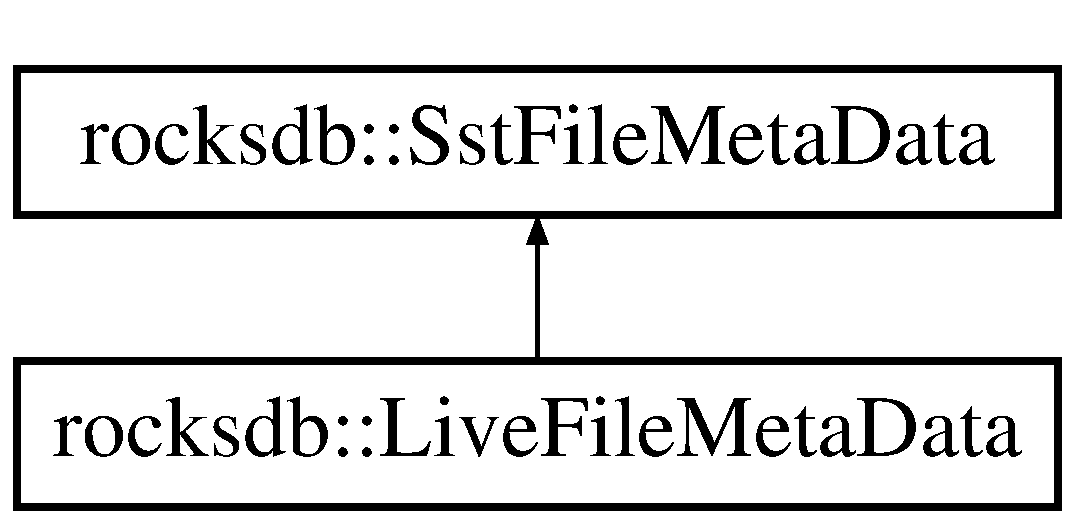
\includegraphics[height=2.000000cm]{structrocksdb_1_1LiveFileMetaData}
\end{center}
\end{figure}
\subsection*{Public Attributes}
\begin{DoxyCompactItemize}
\item 
std\+::string {\bfseries column\+\_\+family\+\_\+name}\hypertarget{structrocksdb_1_1LiveFileMetaData_a23fdc484a64a60650dc81436ddaf679c}{}\label{structrocksdb_1_1LiveFileMetaData_a23fdc484a64a60650dc81436ddaf679c}

\item 
int {\bfseries level}\hypertarget{structrocksdb_1_1LiveFileMetaData_a20f482793b1d9c47e8f141f4efcf5338}{}\label{structrocksdb_1_1LiveFileMetaData_a20f482793b1d9c47e8f141f4efcf5338}

\end{DoxyCompactItemize}
\subsection*{Additional Inherited Members}


The documentation for this struct was generated from the following file\+:\begin{DoxyCompactItemize}
\item 
Appserver/src/external/rocksdb/metadata.\+h\end{DoxyCompactItemize}

\hypertarget{classrocksdb_1_1LogFile}{}\section{rocksdb\+:\+:Log\+File Class Reference}
\label{classrocksdb_1_1LogFile}\index{rocksdb\+::\+Log\+File@{rocksdb\+::\+Log\+File}}
\subsection*{Public Member Functions}
\begin{DoxyCompactItemize}
\item 
virtual std\+::string {\bfseries Path\+Name} () const =0\hypertarget{classrocksdb_1_1LogFile_ad420284dff771d305a7ddbef2a9cdf78}{}\label{classrocksdb_1_1LogFile_ad420284dff771d305a7ddbef2a9cdf78}

\item 
virtual uint64\+\_\+t {\bfseries Log\+Number} () const =0\hypertarget{classrocksdb_1_1LogFile_ac512eef738c0f09c8f019607937e2153}{}\label{classrocksdb_1_1LogFile_ac512eef738c0f09c8f019607937e2153}

\item 
virtual Wal\+File\+Type {\bfseries Type} () const =0\hypertarget{classrocksdb_1_1LogFile_a680e4dd110f67560c473f4a8f66a595f}{}\label{classrocksdb_1_1LogFile_a680e4dd110f67560c473f4a8f66a595f}

\item 
virtual Sequence\+Number {\bfseries Start\+Sequence} () const =0\hypertarget{classrocksdb_1_1LogFile_a2d08d4f965651f916792ca6191f5a1b6}{}\label{classrocksdb_1_1LogFile_a2d08d4f965651f916792ca6191f5a1b6}

\item 
virtual uint64\+\_\+t {\bfseries Size\+File\+Bytes} () const =0\hypertarget{classrocksdb_1_1LogFile_a383bf764f3a5b506089cc585089163fc}{}\label{classrocksdb_1_1LogFile_a383bf764f3a5b506089cc585089163fc}

\end{DoxyCompactItemize}


The documentation for this class was generated from the following file\+:\begin{DoxyCompactItemize}
\item 
Appserver/src/external/rocksdb/transaction\+\_\+log.\+h\end{DoxyCompactItemize}

\hypertarget{classrocksdb_1_1Logger}{}\section{rocksdb\+:\+:Logger Class Reference}
\label{classrocksdb_1_1Logger}\index{rocksdb\+::\+Logger@{rocksdb\+::\+Logger}}
\subsection*{Public Member Functions}
\begin{DoxyCompactItemize}
\item 
{\bfseries Logger} (const Info\+Log\+Level log\+\_\+level=Info\+Log\+Level\+::\+I\+N\+F\+O\+\_\+\+L\+E\+V\+EL)\hypertarget{classrocksdb_1_1Logger_a55e2163280415b50fd691030e6d67f85}{}\label{classrocksdb_1_1Logger_a55e2163280415b50fd691030e6d67f85}

\item 
virtual void {\bfseries Log\+Header} (const char $\ast$format, va\+\_\+list ap)\hypertarget{classrocksdb_1_1Logger_a410df0fed9121f3ea0797d1cfd45c6a5}{}\label{classrocksdb_1_1Logger_a410df0fed9121f3ea0797d1cfd45c6a5}

\item 
virtual void {\bfseries Logv} (const char $\ast$format, va\+\_\+list ap)=0\hypertarget{classrocksdb_1_1Logger_ab122e681ff3273a431853d8abe0adb8b}{}\label{classrocksdb_1_1Logger_ab122e681ff3273a431853d8abe0adb8b}

\item 
virtual void {\bfseries Logv} (const Info\+Log\+Level log\+\_\+level, const char $\ast$format, va\+\_\+list ap)\hypertarget{classrocksdb_1_1Logger_a97320233345b7f1513bbb560b79e906d}{}\label{classrocksdb_1_1Logger_a97320233345b7f1513bbb560b79e906d}

\item 
virtual size\+\_\+t {\bfseries Get\+Log\+File\+Size} () const\hypertarget{classrocksdb_1_1Logger_a61fd491a0af47177b1a7baa4547cfbe4}{}\label{classrocksdb_1_1Logger_a61fd491a0af47177b1a7baa4547cfbe4}

\item 
virtual void {\bfseries Flush} ()\hypertarget{classrocksdb_1_1Logger_aac0bfb0a497280b230bd4acab71fd3ed}{}\label{classrocksdb_1_1Logger_aac0bfb0a497280b230bd4acab71fd3ed}

\item 
virtual Info\+Log\+Level {\bfseries Get\+Info\+Log\+Level} () const\hypertarget{classrocksdb_1_1Logger_a2e87a92355786a15f155ece899acc74d}{}\label{classrocksdb_1_1Logger_a2e87a92355786a15f155ece899acc74d}

\item 
virtual void {\bfseries Set\+Info\+Log\+Level} (const Info\+Log\+Level log\+\_\+level)\hypertarget{classrocksdb_1_1Logger_ad501902d1fc1bcb12593b50e1b38ef85}{}\label{classrocksdb_1_1Logger_ad501902d1fc1bcb12593b50e1b38ef85}

\end{DoxyCompactItemize}
\subsection*{Public Attributes}
\begin{DoxyCompactItemize}
\item 
size\+\_\+t {\bfseries k\+Do\+Not\+Support\+Get\+Log\+File\+Size} = std\+::numeric\+\_\+limits$<$size\+\_\+t$>$\+::max()\hypertarget{classrocksdb_1_1Logger_af3dc2aa3d30220d12e2bcff70be6b2b0}{}\label{classrocksdb_1_1Logger_af3dc2aa3d30220d12e2bcff70be6b2b0}

\end{DoxyCompactItemize}


The documentation for this class was generated from the following file\+:\begin{DoxyCompactItemize}
\item 
Appserver/src/external/rocksdb/env.\+h\end{DoxyCompactItemize}

\hypertarget{classJson_1_1LogicError}{}\section{Json\+:\+:Logic\+Error Class Reference}
\label{classJson_1_1LogicError}\index{Json\+::\+Logic\+Error@{Json\+::\+Logic\+Error}}


{\ttfamily \#include $<$json.\+h$>$}

Inheritance diagram for Json\+:\+:Logic\+Error\+:\begin{figure}[H]
\begin{center}
\leavevmode
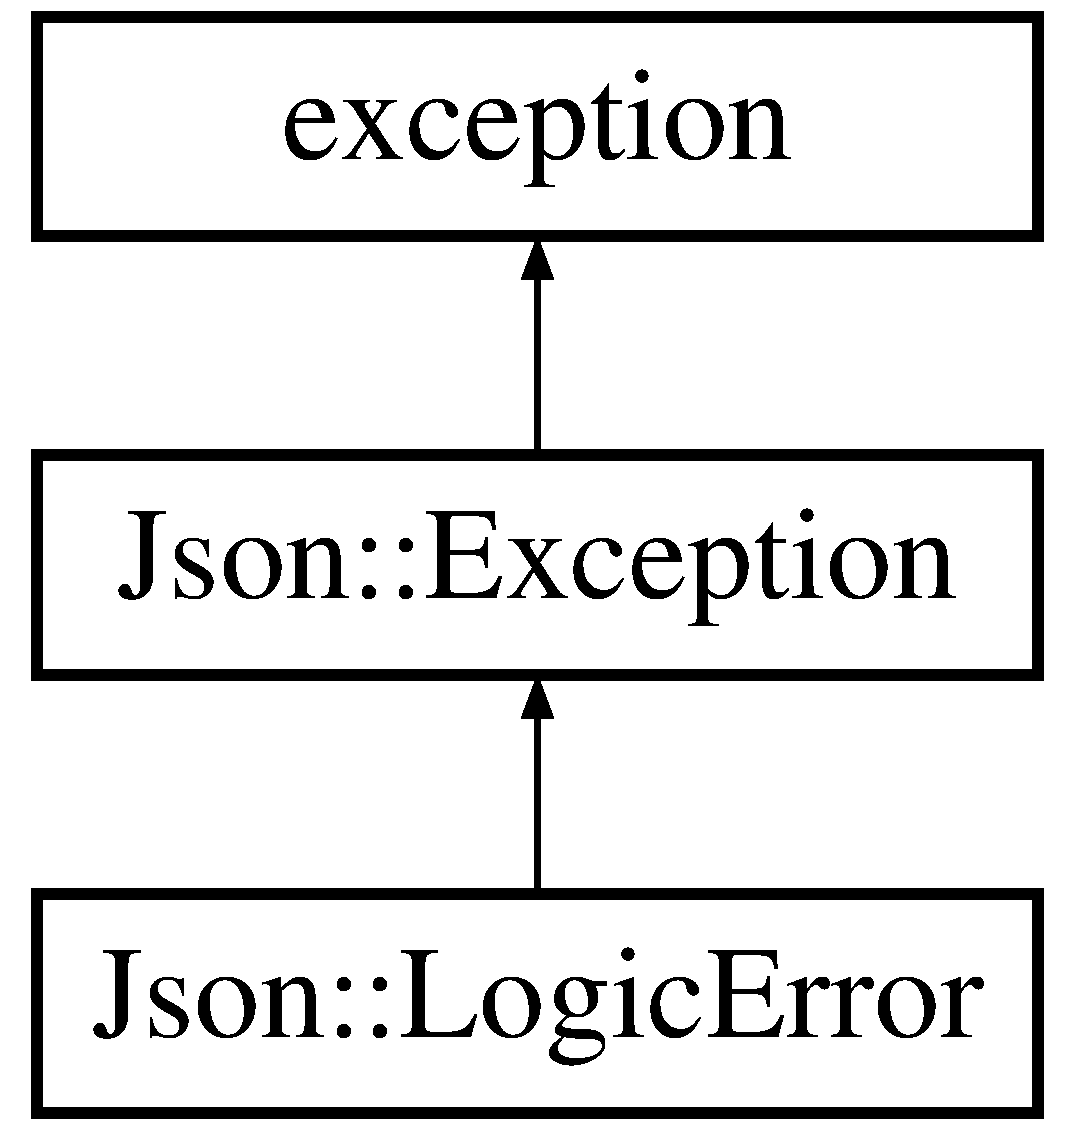
\includegraphics[height=3.000000cm]{classJson_1_1LogicError}
\end{center}
\end{figure}
\subsection*{Public Member Functions}
\begin{DoxyCompactItemize}
\item 
{\bfseries Logic\+Error} (J\+S\+O\+N\+C\+P\+P\+\_\+\+S\+T\+R\+I\+NG const \&msg)\hypertarget{classJson_1_1LogicError_acca679aa49768a4a1de7b705c67c2919}{}\label{classJson_1_1LogicError_acca679aa49768a4a1de7b705c67c2919}

\end{DoxyCompactItemize}
\subsection*{Additional Inherited Members}


\subsection{Detailed Description}
Exceptions thrown by J\+S\+O\+N\+\_\+\+A\+S\+S\+E\+R\+T/\+J\+S\+O\+N\+\_\+\+F\+A\+IL macros.

These are precondition-\/violations (user bugs) and internal errors (our bugs).

\begin{DoxyRemark}{Remarks}
derived from \hyperlink{classJson_1_1Exception}{Json\+::\+Exception} 
\end{DoxyRemark}


The documentation for this class was generated from the following files\+:\begin{DoxyCompactItemize}
\item 
Appserver/src/external/json/json.\+h\item 
Appserver/src/external/json/jsoncpp.\+cpp\end{DoxyCompactItemize}

\hypertarget{classrocksdb_1_1ManagedSnapshot}{}\section{rocksdb\+:\+:Managed\+Snapshot Class Reference}
\label{classrocksdb_1_1ManagedSnapshot}\index{rocksdb\+::\+Managed\+Snapshot@{rocksdb\+::\+Managed\+Snapshot}}
\subsection*{Public Member Functions}
\begin{DoxyCompactItemize}
\item 
{\bfseries Managed\+Snapshot} (\hyperlink{classrocksdb_1_1DB}{DB} $\ast$db)\hypertarget{classrocksdb_1_1ManagedSnapshot_ad1906cef031ba6c14d6d46bcf0a81983}{}\label{classrocksdb_1_1ManagedSnapshot_ad1906cef031ba6c14d6d46bcf0a81983}

\item 
{\bfseries Managed\+Snapshot} (\hyperlink{classrocksdb_1_1DB}{DB} $\ast$db, const \hyperlink{classrocksdb_1_1Snapshot}{Snapshot} $\ast$\+\_\+snapshot)\hypertarget{classrocksdb_1_1ManagedSnapshot_a32c15ed8e364116f9390567f0395509e}{}\label{classrocksdb_1_1ManagedSnapshot_a32c15ed8e364116f9390567f0395509e}

\item 
const \hyperlink{classrocksdb_1_1Snapshot}{Snapshot} $\ast$ {\bfseries snapshot} ()\hypertarget{classrocksdb_1_1ManagedSnapshot_ab82cf7752fb1fe14bfef62d03b2f4a2c}{}\label{classrocksdb_1_1ManagedSnapshot_ab82cf7752fb1fe14bfef62d03b2f4a2c}

\end{DoxyCompactItemize}


The documentation for this class was generated from the following file\+:\begin{DoxyCompactItemize}
\item 
Appserver/src/external/rocksdb/snapshot.\+h\end{DoxyCompactItemize}

\hypertarget{classManejadorDeConexiones}{}\section{Manejador\+De\+Conexiones Class Reference}
\label{classManejadorDeConexiones}\index{Manejador\+De\+Conexiones@{Manejador\+De\+Conexiones}}
\subsection*{Public Member Functions}
\begin{DoxyCompactItemize}
\item 
void {\bfseries iniciar\+Conexion\+Como\+Servidor} (string puerto, \hyperlink{classServidor}{Servidor} $\ast$servidor)\hypertarget{classManejadorDeConexiones_a66bae5cdd4959f6cc555534749b3ebb1}{}\label{classManejadorDeConexiones_a66bae5cdd4959f6cc555534749b3ebb1}

\item 
void {\bfseries terminar\+Conexion\+Como\+Servidor} ()\hypertarget{classManejadorDeConexiones_a8e26d47396e240d2c891b0c14a6ca321}{}\label{classManejadorDeConexiones_a8e26d47396e240d2c891b0c14a6ca321}

\item 
\hyperlink{classMensajeHTTPReply}{Mensaje\+H\+T\+T\+P\+Reply} {\bfseries enviar\+Mensaje\+H\+T\+TP} (\hyperlink{classMensajeHTTPRequest}{Mensaje\+H\+T\+T\+P\+Request} $\ast$request, string puerto\+Local)\hypertarget{classManejadorDeConexiones_a5ddc9c13584c9ccdda092c2330e1856b}{}\label{classManejadorDeConexiones_a5ddc9c13584c9ccdda092c2330e1856b}

\end{DoxyCompactItemize}


The documentation for this class was generated from the following files\+:\begin{DoxyCompactItemize}
\item 
Appserver/src/servicios/Manejador\+De\+Conexiones.\+h\item 
Appserver/src/servicios/Manejador\+De\+Conexiones.\+cpp\end{DoxyCompactItemize}

\hypertarget{structmbuf}{}\section{mbuf Struct Reference}
\label{structmbuf}\index{mbuf@{mbuf}}
\subsection*{Public Attributes}
\begin{DoxyCompactItemize}
\item 
char $\ast$ {\bfseries buf}\hypertarget{structmbuf_ae2a6e23a4997e9aea0908628db2b23d0}{}\label{structmbuf_ae2a6e23a4997e9aea0908628db2b23d0}

\item 
size\+\_\+t {\bfseries len}\hypertarget{structmbuf_a4da00860609dd46fe8b679d5e1deeac3}{}\label{structmbuf_a4da00860609dd46fe8b679d5e1deeac3}

\item 
size\+\_\+t {\bfseries size}\hypertarget{structmbuf_ae245d03a50c2891c1fb228093d842270}{}\label{structmbuf_ae245d03a50c2891c1fb228093d842270}

\end{DoxyCompactItemize}


The documentation for this struct was generated from the following file\+:\begin{DoxyCompactItemize}
\item 
Appserver/src/external/mongoose/mongoose.\+h\end{DoxyCompactItemize}

\hypertarget{structMD5Context}{}\section{M\+D5\+Context Struct Reference}
\label{structMD5Context}\index{M\+D5\+Context@{M\+D5\+Context}}
\subsection*{Public Attributes}
\begin{DoxyCompactItemize}
\item 
uint32\+\_\+t {\bfseries buf} \mbox{[}4\mbox{]}\hypertarget{structMD5Context_a6129b10b90387e1cb1d4cd92e4605c33}{}\label{structMD5Context_a6129b10b90387e1cb1d4cd92e4605c33}

\item 
uint32\+\_\+t {\bfseries bits} \mbox{[}2\mbox{]}\hypertarget{structMD5Context_a48f837fb64afd013f832e3cdab68e5de}{}\label{structMD5Context_a48f837fb64afd013f832e3cdab68e5de}

\item 
unsigned char {\bfseries in} \mbox{[}64\mbox{]}\hypertarget{structMD5Context_ae8be45f236e5cb12b0ae79da77e5f929}{}\label{structMD5Context_ae8be45f236e5cb12b0ae79da77e5f929}

\end{DoxyCompactItemize}


The documentation for this struct was generated from the following file\+:\begin{DoxyCompactItemize}
\item 
Appserver/src/external/mongoose/mongoose.\+h\end{DoxyCompactItemize}

\hypertarget{classrocksdb_1_1MemoryUtil}{}\section{rocksdb\+:\+:Memory\+Util Class Reference}
\label{classrocksdb_1_1MemoryUtil}\index{rocksdb\+::\+Memory\+Util@{rocksdb\+::\+Memory\+Util}}
\subsection*{Public Types}
\begin{DoxyCompactItemize}
\item 
enum {\bfseries Usage\+Type} \+: int \{ \\*
{\bfseries k\+Mem\+Table\+Total} = 0, 
{\bfseries k\+Mem\+Table\+Un\+Flushed} = 1, 
{\bfseries k\+Table\+Readers\+Total} = 2, 
{\bfseries k\+Cache\+Total} = 3, 
\\*
{\bfseries k\+Num\+Usage\+Types} = 4
 \}\hypertarget{classrocksdb_1_1MemoryUtil_af3650e6ec0c037d1c973d43c75a18f60}{}\label{classrocksdb_1_1MemoryUtil_af3650e6ec0c037d1c973d43c75a18f60}

\end{DoxyCompactItemize}
\subsection*{Static Public Member Functions}
\begin{DoxyCompactItemize}
\item 
static \hyperlink{classrocksdb_1_1Status}{Status} {\bfseries Get\+Approximate\+Memory\+Usage\+By\+Type} (const std\+::vector$<$ \hyperlink{classrocksdb_1_1DB}{DB} $\ast$$>$ \&dbs, const std\+::unordered\+\_\+set$<$ const \hyperlink{classrocksdb_1_1Cache}{Cache} $\ast$$>$ cache\+\_\+set, std\+::map$<$ Memory\+Util\+::\+Usage\+Type, uint64\+\_\+t $>$ $\ast$usage\+\_\+by\+\_\+type)\hypertarget{classrocksdb_1_1MemoryUtil_af042daefc894bd4f2f4109649be96aec}{}\label{classrocksdb_1_1MemoryUtil_af042daefc894bd4f2f4109649be96aec}

\end{DoxyCompactItemize}


The documentation for this class was generated from the following file\+:\begin{DoxyCompactItemize}
\item 
Appserver/src/external/rocksdb/utilities/memory\+\_\+util.\+h\end{DoxyCompactItemize}

\hypertarget{classrocksdb_1_1MemTableRep}{}\section{rocksdb\+:\+:Mem\+Table\+Rep Class Reference}
\label{classrocksdb_1_1MemTableRep}\index{rocksdb\+::\+Mem\+Table\+Rep@{rocksdb\+::\+Mem\+Table\+Rep}}
\subsection*{Classes}
\begin{DoxyCompactItemize}
\item 
class \hyperlink{classrocksdb_1_1MemTableRep_1_1Iterator}{Iterator}
\item 
class \hyperlink{classrocksdb_1_1MemTableRep_1_1KeyComparator}{Key\+Comparator}
\end{DoxyCompactItemize}
\subsection*{Public Member Functions}
\begin{DoxyCompactItemize}
\item 
{\bfseries Mem\+Table\+Rep} (Mem\+Table\+Allocator $\ast$allocator)\hypertarget{classrocksdb_1_1MemTableRep_a40f57aa1059c416c706f44bd0573062b}{}\label{classrocksdb_1_1MemTableRep_a40f57aa1059c416c706f44bd0573062b}

\item 
virtual Key\+Handle {\bfseries Allocate} (const size\+\_\+t len, char $\ast$$\ast$buf)\hypertarget{classrocksdb_1_1MemTableRep_a6c355ad7a8a4163c6da861fcd2e9e1c1}{}\label{classrocksdb_1_1MemTableRep_a6c355ad7a8a4163c6da861fcd2e9e1c1}

\item 
virtual void {\bfseries Insert} (Key\+Handle handle)=0\hypertarget{classrocksdb_1_1MemTableRep_a16ea561f3ad9fa8a7817081f41a5bc6f}{}\label{classrocksdb_1_1MemTableRep_a16ea561f3ad9fa8a7817081f41a5bc6f}

\item 
virtual void {\bfseries Insert\+Concurrently} (Key\+Handle handle)\hypertarget{classrocksdb_1_1MemTableRep_a4bc4b4bc476d9aee29a381ee94256003}{}\label{classrocksdb_1_1MemTableRep_a4bc4b4bc476d9aee29a381ee94256003}

\item 
virtual bool {\bfseries Contains} (const char $\ast$key) const =0\hypertarget{classrocksdb_1_1MemTableRep_a9680af59089a57d48e65305181af275a}{}\label{classrocksdb_1_1MemTableRep_a9680af59089a57d48e65305181af275a}

\item 
virtual void {\bfseries Mark\+Read\+Only} ()\hypertarget{classrocksdb_1_1MemTableRep_a8bada15fbc6e474c3cdd25ba739b47b3}{}\label{classrocksdb_1_1MemTableRep_a8bada15fbc6e474c3cdd25ba739b47b3}

\item 
virtual void {\bfseries Get} (const Lookup\+Key \&k, void $\ast$callback\+\_\+args, bool($\ast$callback\+\_\+func)(void $\ast$arg, const char $\ast$entry))\hypertarget{classrocksdb_1_1MemTableRep_a6822dec90fff8e8048089f219529c952}{}\label{classrocksdb_1_1MemTableRep_a6822dec90fff8e8048089f219529c952}

\item 
virtual uint64\+\_\+t {\bfseries Approximate\+Num\+Entries} (const \hyperlink{classrocksdb_1_1Slice}{Slice} \&start\+\_\+ikey, const \hyperlink{classrocksdb_1_1Slice}{Slice} \&end\+\_\+key)\hypertarget{classrocksdb_1_1MemTableRep_a9ddecdf2ae912245236f170cd08e22b9}{}\label{classrocksdb_1_1MemTableRep_a9ddecdf2ae912245236f170cd08e22b9}

\item 
virtual size\+\_\+t {\bfseries Approximate\+Memory\+Usage} ()=0\hypertarget{classrocksdb_1_1MemTableRep_a5a313a7730104e94f4c60e0cf2818241}{}\label{classrocksdb_1_1MemTableRep_a5a313a7730104e94f4c60e0cf2818241}

\item 
virtual \hyperlink{classrocksdb_1_1MemTableRep_1_1Iterator}{Iterator} $\ast$ {\bfseries Get\+Iterator} (Arena $\ast$arena=nullptr)=0\hypertarget{classrocksdb_1_1MemTableRep_a512847e7a3f7b77f738c97a04b92ef44}{}\label{classrocksdb_1_1MemTableRep_a512847e7a3f7b77f738c97a04b92ef44}

\item 
virtual \hyperlink{classrocksdb_1_1MemTableRep_1_1Iterator}{Iterator} $\ast$ {\bfseries Get\+Dynamic\+Prefix\+Iterator} (Arena $\ast$arena=nullptr)\hypertarget{classrocksdb_1_1MemTableRep_a1d2ba3bbc72fa104828a7df394fb0d22}{}\label{classrocksdb_1_1MemTableRep_a1d2ba3bbc72fa104828a7df394fb0d22}

\item 
virtual bool {\bfseries Is\+Merge\+Operator\+Supported} () const\hypertarget{classrocksdb_1_1MemTableRep_a32a54039ec9337b1449b2fb02c7b32f1}{}\label{classrocksdb_1_1MemTableRep_a32a54039ec9337b1449b2fb02c7b32f1}

\item 
virtual bool {\bfseries Is\+Snapshot\+Supported} () const\hypertarget{classrocksdb_1_1MemTableRep_a808715ac901ddabeb55afdee56df4867}{}\label{classrocksdb_1_1MemTableRep_a808715ac901ddabeb55afdee56df4867}

\end{DoxyCompactItemize}
\subsection*{Protected Member Functions}
\begin{DoxyCompactItemize}
\item 
virtual \hyperlink{classrocksdb_1_1Slice}{Slice} {\bfseries User\+Key} (const char $\ast$key) const\hypertarget{classrocksdb_1_1MemTableRep_a7879bba15f89e0af854770e955839fe0}{}\label{classrocksdb_1_1MemTableRep_a7879bba15f89e0af854770e955839fe0}

\end{DoxyCompactItemize}
\subsection*{Protected Attributes}
\begin{DoxyCompactItemize}
\item 
Mem\+Table\+Allocator $\ast$ {\bfseries allocator\+\_\+}\hypertarget{classrocksdb_1_1MemTableRep_a100849cbb84764e4b83cbaf8fc54a2d6}{}\label{classrocksdb_1_1MemTableRep_a100849cbb84764e4b83cbaf8fc54a2d6}

\end{DoxyCompactItemize}


The documentation for this class was generated from the following file\+:\begin{DoxyCompactItemize}
\item 
Appserver/src/external/rocksdb/memtablerep.\+h\end{DoxyCompactItemize}

\hypertarget{classrocksdb_1_1MemTableRepFactory}{}\section{rocksdb\+:\+:Mem\+Table\+Rep\+Factory Class Reference}
\label{classrocksdb_1_1MemTableRepFactory}\index{rocksdb\+::\+Mem\+Table\+Rep\+Factory@{rocksdb\+::\+Mem\+Table\+Rep\+Factory}}
Inheritance diagram for rocksdb\+:\+:Mem\+Table\+Rep\+Factory\+:\begin{figure}[H]
\begin{center}
\leavevmode
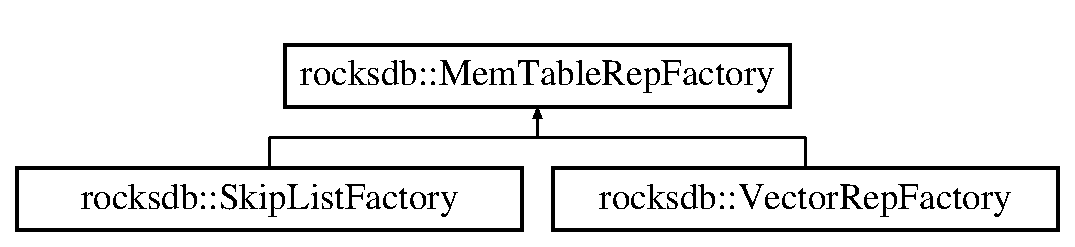
\includegraphics[height=2.000000cm]{classrocksdb_1_1MemTableRepFactory}
\end{center}
\end{figure}
\subsection*{Public Member Functions}
\begin{DoxyCompactItemize}
\item 
virtual \hyperlink{classrocksdb_1_1MemTableRep}{Mem\+Table\+Rep} $\ast$ {\bfseries Create\+Mem\+Table\+Rep} (const \hyperlink{classrocksdb_1_1MemTableRep_1_1KeyComparator}{Mem\+Table\+Rep\+::\+Key\+Comparator} \&, Mem\+Table\+Allocator $\ast$, const \hyperlink{classrocksdb_1_1SliceTransform}{Slice\+Transform} $\ast$, \hyperlink{classrocksdb_1_1Logger}{Logger} $\ast$logger)=0\hypertarget{classrocksdb_1_1MemTableRepFactory_a87a40d71a4ef4af55eb97ca0da7506fb}{}\label{classrocksdb_1_1MemTableRepFactory_a87a40d71a4ef4af55eb97ca0da7506fb}

\item 
virtual const char $\ast$ {\bfseries Name} () const =0\hypertarget{classrocksdb_1_1MemTableRepFactory_ab2d3393c71b0e230c7b68efe8e789bea}{}\label{classrocksdb_1_1MemTableRepFactory_ab2d3393c71b0e230c7b68efe8e789bea}

\item 
virtual bool {\bfseries Is\+Insert\+Concurrently\+Supported} () const\hypertarget{classrocksdb_1_1MemTableRepFactory_a4157b1b98dcb4e2e7f0e5d41aa1025b4}{}\label{classrocksdb_1_1MemTableRepFactory_a4157b1b98dcb4e2e7f0e5d41aa1025b4}

\end{DoxyCompactItemize}


The documentation for this class was generated from the following file\+:\begin{DoxyCompactItemize}
\item 
Appserver/src/external/rocksdb/memtablerep.\+h\end{DoxyCompactItemize}

\hypertarget{classMensajeHTTP}{}\section{Mensaje\+H\+T\+TP Class Reference}
\label{classMensajeHTTP}\index{Mensaje\+H\+T\+TP@{Mensaje\+H\+T\+TP}}
Inheritance diagram for Mensaje\+H\+T\+TP\+:\begin{figure}[H]
\begin{center}
\leavevmode
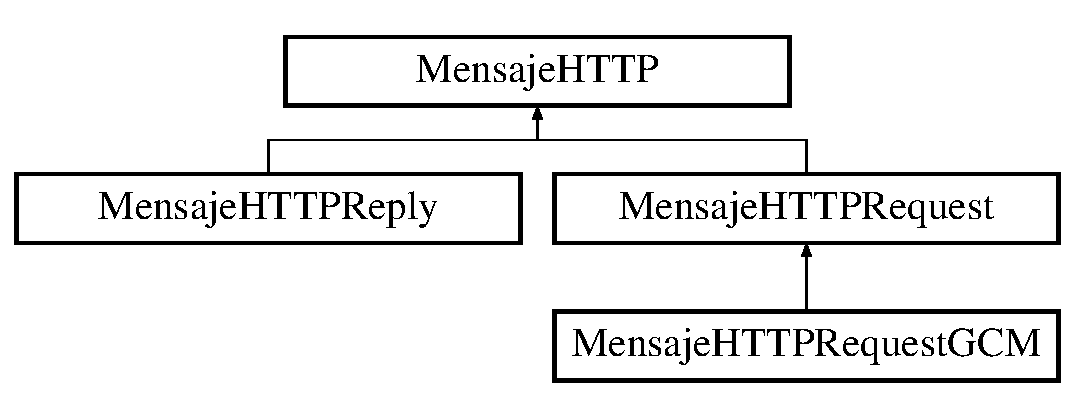
\includegraphics[height=3.000000cm]{classMensajeHTTP}
\end{center}
\end{figure}
\subsection*{Public Member Functions}
\begin{DoxyCompactItemize}
\item 
{\bfseries Mensaje\+H\+T\+TP} (\hyperlink{structhttp__message}{http\+\_\+message} $\ast$mensaje\+MG)\hypertarget{classMensajeHTTP_a81014d5d4ff6304f73ae8ca79e6afc1d}{}\label{classMensajeHTTP_a81014d5d4ff6304f73ae8ca79e6afc1d}

\item 
bool {\bfseries tiene\+Header} (string header)\hypertarget{classMensajeHTTP_ae287891749d61472d882403a9a89d0a4}{}\label{classMensajeHTTP_ae287891749d61472d882403a9a89d0a4}

\item 
string {\bfseries get\+Header} (string header)\hypertarget{classMensajeHTTP_a2bc7778920edd7b85ded455ca16098b7}{}\label{classMensajeHTTP_a2bc7778920edd7b85ded455ca16098b7}

\item 
string {\bfseries get\+Body} ()\hypertarget{classMensajeHTTP_a3a4ae2f0872d7fd3662cc93ebfc12c65}{}\label{classMensajeHTTP_a3a4ae2f0872d7fd3662cc93ebfc12c65}

\item 
void {\bfseries set\+Body} (string body)\hypertarget{classMensajeHTTP_a0797090e1196d3d43b2f7484525d81c2}{}\label{classMensajeHTTP_a0797090e1196d3d43b2f7484525d81c2}

\item 
void {\bfseries agregar\+Header} (string header, string valor)\hypertarget{classMensajeHTTP_af1e394fc2962d285424a94bb7c290a4c}{}\label{classMensajeHTTP_af1e394fc2962d285424a94bb7c290a4c}

\item 
virtual string {\bfseries to\+String} ()=0\hypertarget{classMensajeHTTP_aa24169ae958f27977b3345cf2bb162e3}{}\label{classMensajeHTTP_aa24169ae958f27977b3345cf2bb162e3}

\end{DoxyCompactItemize}
\subsection*{Protected Member Functions}
\begin{DoxyCompactItemize}
\item 
void {\bfseries cargar\+Headers} (\hyperlink{structhttp__message}{http\+\_\+message} $\ast$mensaje\+MG)\hypertarget{classMensajeHTTP_a8f1cf1e316cf0e690c4997262301c8b0}{}\label{classMensajeHTTP_a8f1cf1e316cf0e690c4997262301c8b0}

\item 
string {\bfseries mg\+\_\+str\+To\+String} (\hyperlink{structmg__str}{mg\+\_\+str} \&mg\+Str)\hypertarget{classMensajeHTTP_a5b13801cd2ea67aec646315661c9c7d5}{}\label{classMensajeHTTP_a5b13801cd2ea67aec646315661c9c7d5}

\item 
string {\bfseries headers\+To\+String} ()\hypertarget{classMensajeHTTP_acac8b954266349e08823a5b036b7b28d}{}\label{classMensajeHTTP_acac8b954266349e08823a5b036b7b28d}

\end{DoxyCompactItemize}
\subsection*{Protected Attributes}
\begin{DoxyCompactItemize}
\item 
string {\bfseries body}\hypertarget{classMensajeHTTP_a4dfdf400c066b6f55d29986feff110c9}{}\label{classMensajeHTTP_a4dfdf400c066b6f55d29986feff110c9}

\item 
map$<$ string, string $>$ {\bfseries headers}\hypertarget{classMensajeHTTP_a3f3375d37fcec2dec4562119408ca4a5}{}\label{classMensajeHTTP_a3f3375d37fcec2dec4562119408ca4a5}

\end{DoxyCompactItemize}


The documentation for this class was generated from the following files\+:\begin{DoxyCompactItemize}
\item 
Appserver/src/servicios/Mensaje\+H\+T\+T\+P.\+h\item 
Appserver/src/servicios/Mensaje\+H\+T\+T\+P.\+cpp\end{DoxyCompactItemize}

\hypertarget{classMensajeHTTPReply}{}\section{Mensaje\+H\+T\+T\+P\+Reply Class Reference}
\label{classMensajeHTTPReply}\index{Mensaje\+H\+T\+T\+P\+Reply@{Mensaje\+H\+T\+T\+P\+Reply}}
Inheritance diagram for Mensaje\+H\+T\+T\+P\+Reply\+:\begin{figure}[H]
\begin{center}
\leavevmode
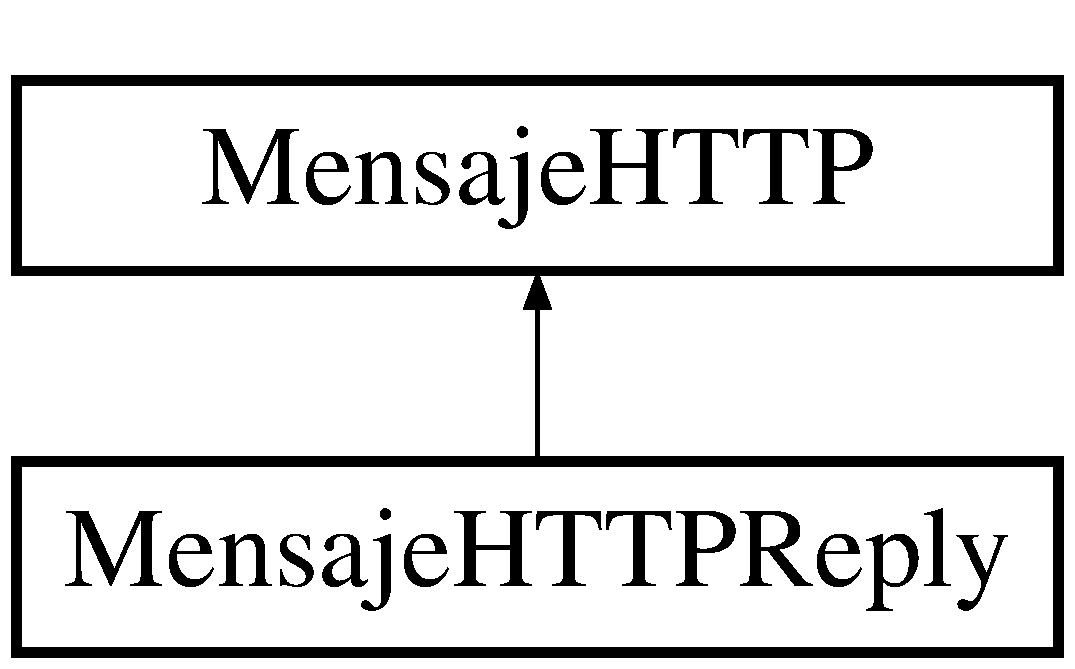
\includegraphics[height=2.000000cm]{classMensajeHTTPReply}
\end{center}
\end{figure}
\subsection*{Public Member Functions}
\begin{DoxyCompactItemize}
\item 
{\bfseries Mensaje\+H\+T\+T\+P\+Reply} (\hyperlink{structhttp__message}{http\+\_\+message} $\ast$mensaje\+MG)\hypertarget{classMensajeHTTPReply_a6c8940c801dd402d16ea10d4ca82af0f}{}\label{classMensajeHTTPReply_a6c8940c801dd402d16ea10d4ca82af0f}

\item 
void {\bfseries set\+Codigo} (int codigo)\hypertarget{classMensajeHTTPReply_a7b53a4451eceaf625243229dfff4a4e1}{}\label{classMensajeHTTPReply_a7b53a4451eceaf625243229dfff4a4e1}

\item 
int {\bfseries get\+Codigo} ()\hypertarget{classMensajeHTTPReply_a1b3a8cc18ee5f15a3444859c36c86e7f}{}\label{classMensajeHTTPReply_a1b3a8cc18ee5f15a3444859c36c86e7f}

\item 
void {\bfseries set\+Mensaje\+De\+Estado} (string mensaje)\hypertarget{classMensajeHTTPReply_abeee087f10205a27689c11134af41053}{}\label{classMensajeHTTPReply_abeee087f10205a27689c11134af41053}

\item 
string {\bfseries get\+Mensaje\+De\+Estado} ()\hypertarget{classMensajeHTTPReply_a5a9a80b64a8c0f9bf76fbd7917bd8323}{}\label{classMensajeHTTPReply_a5a9a80b64a8c0f9bf76fbd7917bd8323}

\item 
string {\bfseries to\+String} ()\hypertarget{classMensajeHTTPReply_a95c2acf562527553dc7218827c3d2049}{}\label{classMensajeHTTPReply_a95c2acf562527553dc7218827c3d2049}

\end{DoxyCompactItemize}
\subsection*{Additional Inherited Members}


The documentation for this class was generated from the following files\+:\begin{DoxyCompactItemize}
\item 
Appserver/src/servicios/Mensaje\+H\+T\+T\+P\+Reply.\+h\item 
Appserver/src/servicios/Mensaje\+H\+T\+T\+P\+Reply.\+cpp\end{DoxyCompactItemize}

\hypertarget{classMensajeHTTPRequest}{}\section{Mensaje\+H\+T\+T\+P\+Request Class Reference}
\label{classMensajeHTTPRequest}\index{Mensaje\+H\+T\+T\+P\+Request@{Mensaje\+H\+T\+T\+P\+Request}}
Inheritance diagram for Mensaje\+H\+T\+T\+P\+Request\+:\begin{figure}[H]
\begin{center}
\leavevmode
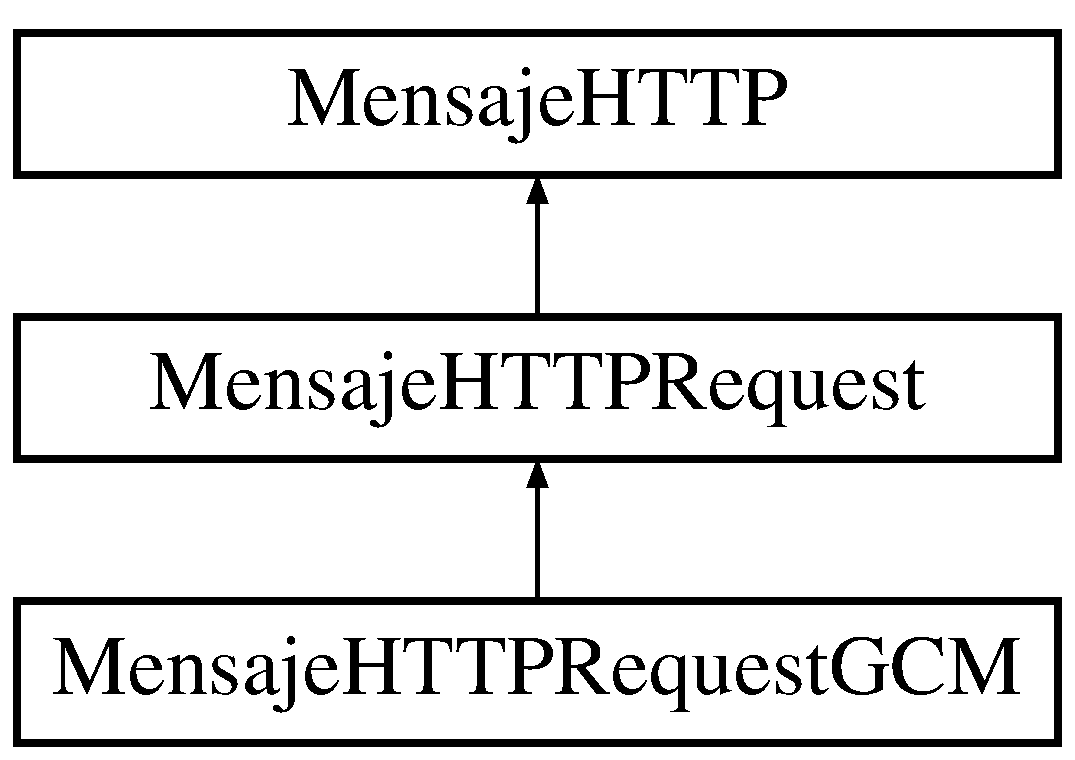
\includegraphics[height=3.000000cm]{classMensajeHTTPRequest}
\end{center}
\end{figure}
\subsection*{Public Member Functions}
\begin{DoxyCompactItemize}
\item 
{\bfseries Mensaje\+H\+T\+T\+P\+Request} (\hyperlink{structhttp__message}{http\+\_\+message} $\ast$mensaje\+MG)\hypertarget{classMensajeHTTPRequest_a0d073186e943c4495fd6d3d9d9422fa5}{}\label{classMensajeHTTPRequest_a0d073186e943c4495fd6d3d9d9422fa5}

\item 
string {\bfseries get\+Metodo} ()\hypertarget{classMensajeHTTPRequest_a977e087f696316a18d66c0caf6efbd96}{}\label{classMensajeHTTPRequest_a977e087f696316a18d66c0caf6efbd96}

\item 
string {\bfseries get\+U\+RI} ()\hypertarget{classMensajeHTTPRequest_a29e2bd2380e8f4e3be66a4695af60c82}{}\label{classMensajeHTTPRequest_a29e2bd2380e8f4e3be66a4695af60c82}

\item 
string {\bfseries to\+String} ()\hypertarget{classMensajeHTTPRequest_a7b1f874c87b76188e7c76eeea5b9e281}{}\label{classMensajeHTTPRequest_a7b1f874c87b76188e7c76eeea5b9e281}

\item 
void {\bfseries set\+Metodo} (string metodo)\hypertarget{classMensajeHTTPRequest_a3ecb30dba9bb014cde0599f4c3950743}{}\label{classMensajeHTTPRequest_a3ecb30dba9bb014cde0599f4c3950743}

\item 
void {\bfseries set\+U\+RI} (string uri)\hypertarget{classMensajeHTTPRequest_a3dc7c23432fd17d0a5d820e05eff0708}{}\label{classMensajeHTTPRequest_a3dc7c23432fd17d0a5d820e05eff0708}

\end{DoxyCompactItemize}
\subsection*{Additional Inherited Members}


The documentation for this class was generated from the following files\+:\begin{DoxyCompactItemize}
\item 
Appserver/src/servicios/Mensaje\+H\+T\+T\+P\+Request.\+h\item 
Appserver/src/servicios/Mensaje\+H\+T\+T\+P\+Request.\+cpp\end{DoxyCompactItemize}

\hypertarget{classMensajeHTTPRequestGCM}{}\section{Mensaje\+H\+T\+T\+P\+Request\+G\+CM Class Reference}
\label{classMensajeHTTPRequestGCM}\index{Mensaje\+H\+T\+T\+P\+Request\+G\+CM@{Mensaje\+H\+T\+T\+P\+Request\+G\+CM}}
Inheritance diagram for Mensaje\+H\+T\+T\+P\+Request\+G\+CM\+:\begin{figure}[H]
\begin{center}
\leavevmode
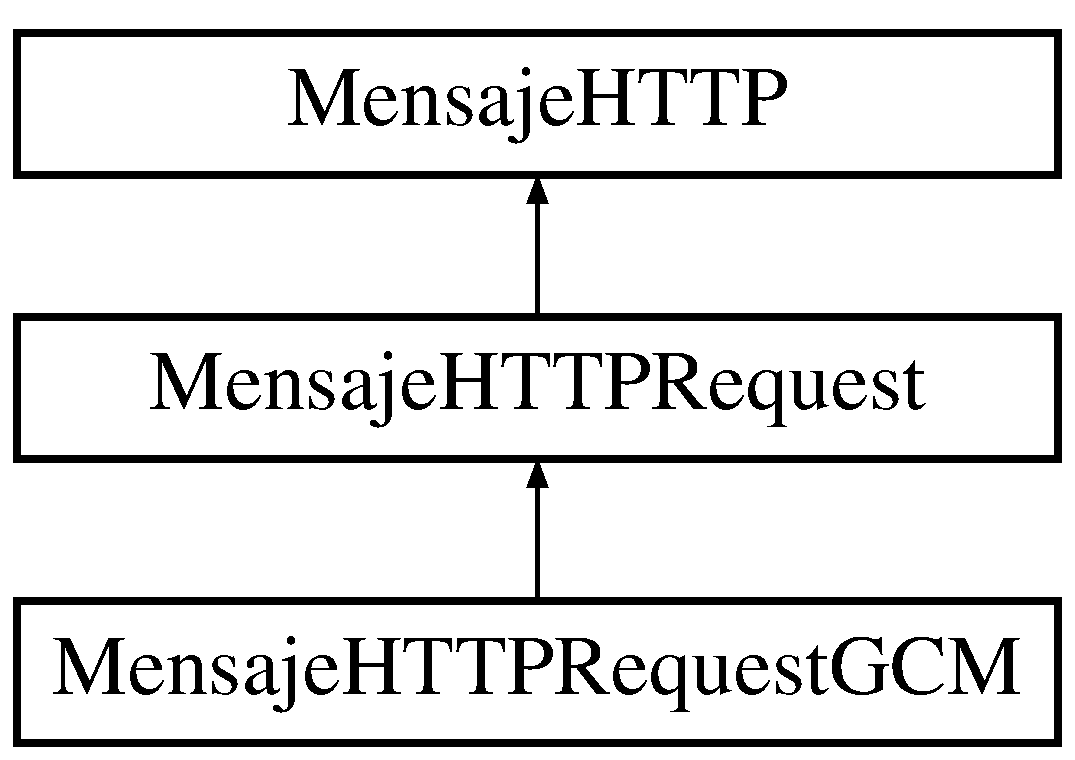
\includegraphics[height=3.000000cm]{classMensajeHTTPRequestGCM}
\end{center}
\end{figure}
\subsection*{Additional Inherited Members}


The documentation for this class was generated from the following files\+:\begin{DoxyCompactItemize}
\item 
Appserver/src/servicios/Mensaje\+H\+T\+T\+P\+Request\+G\+C\+M.\+h\item 
Appserver/src/servicios/Mensaje\+H\+T\+T\+P\+Request\+G\+C\+M.\+cpp\end{DoxyCompactItemize}

\hypertarget{classMensajero}{}\section{Mensajero Class Reference}
\label{classMensajero}\index{Mensajero@{Mensajero}}
\subsection*{Public Member Functions}
\begin{DoxyCompactItemize}
\item 
{\bfseries Mensajero} (\hyperlink{classManejadorDeConexiones}{Manejador\+De\+Conexiones} $\ast$conexiones, \hyperlink{classSesionesDeUsuarios}{Sesiones\+De\+Usuarios} $\ast$sesiones)\hypertarget{classMensajero_ac8f85b51bc31c39fe64e04d0fd07326e}{}\label{classMensajero_ac8f85b51bc31c39fe64e04d0fd07326e}

\item 
bool {\bfseries enviar\+Mensaje} (string emisor, string receptor, string mensaje)\hypertarget{classMensajero_a44f018371a6652717570ec1f003fc35a}{}\label{classMensajero_a44f018371a6652717570ec1f003fc35a}

\item 
bool {\bfseries notificar\+Usuario\+Sobre\+Match\+Con} (string usuario, string match)\hypertarget{classMensajero_a2df6b87ba2bc3c57200b2913d965a083}{}\label{classMensajero_a2df6b87ba2bc3c57200b2913d965a083}

\end{DoxyCompactItemize}


The documentation for this class was generated from the following files\+:\begin{DoxyCompactItemize}
\item 
Appserver/src/servicios/Mensajero.\+h\item 
Appserver/src/servicios/Mensajero.\+cpp\end{DoxyCompactItemize}

\hypertarget{classMensajes}{}\section{Mensajes Class Reference}
\label{classMensajes}\index{Mensajes@{Mensajes}}
\subsection*{Public Member Functions}
\begin{DoxyCompactItemize}
\item 
{\bfseries Mensajes} (string json\+Texto)\hypertarget{classMensajes_a024b1e59811c21e05e2a5fbe8f8ddfd2}{}\label{classMensajes_a024b1e59811c21e05e2a5fbe8f8ddfd2}

\item 
string {\bfseries get\+Emisor} (int nro\+Mensaje)\hypertarget{classMensajes_aafaa164b11c9afd52a27bd64be3f847e}{}\label{classMensajes_aafaa164b11c9afd52a27bd64be3f847e}

\item 
string {\bfseries get\+Mensaje} (int nro\+Mensaje)\hypertarget{classMensajes_a635b359e1f79ffcf0ecd3931524f4df7}{}\label{classMensajes_a635b359e1f79ffcf0ecd3931524f4df7}

\item 
string {\bfseries to\+String} ()\hypertarget{classMensajes_a1b69bfdd70493bfa3e5fde215e881636}{}\label{classMensajes_a1b69bfdd70493bfa3e5fde215e881636}

\item 
int {\bfseries get\+Tamanio} ()\hypertarget{classMensajes_abb73e0ae442301ff55f77121432572dc}{}\label{classMensajes_abb73e0ae442301ff55f77121432572dc}

\item 
void {\bfseries agregar\+Mensaje} (string emisor, string mensaje)\hypertarget{classMensajes_ac9cef976098cfebde8e682bdd91d6695}{}\label{classMensajes_ac9cef976098cfebde8e682bdd91d6695}

\end{DoxyCompactItemize}


The documentation for this class was generated from the following files\+:\begin{DoxyCompactItemize}
\item 
Appserver/src/servicios/Mensajes.\+h\item 
Appserver/src/servicios/Mensajes.\+cpp\end{DoxyCompactItemize}

\hypertarget{classrocksdb_1_1MergeOperator}{}\section{rocksdb\+:\+:Merge\+Operator Class Reference}
\label{classrocksdb_1_1MergeOperator}\index{rocksdb\+::\+Merge\+Operator@{rocksdb\+::\+Merge\+Operator}}
Inheritance diagram for rocksdb\+:\+:Merge\+Operator\+:\begin{figure}[H]
\begin{center}
\leavevmode
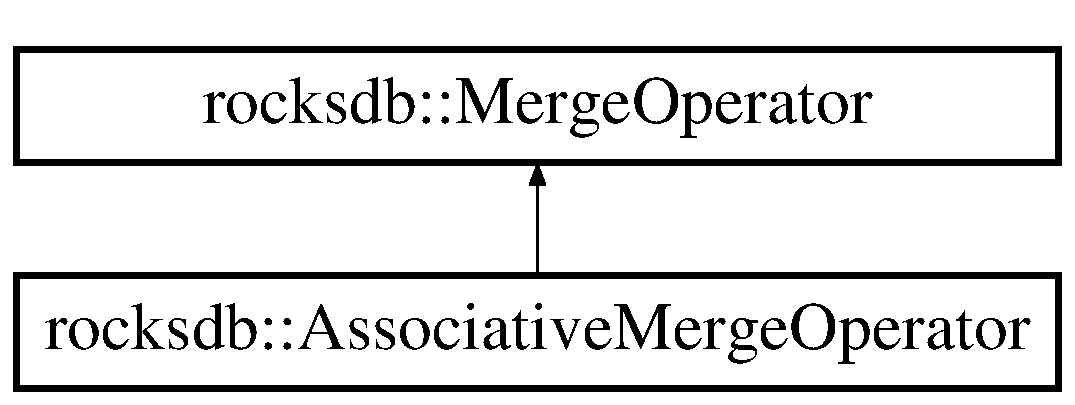
\includegraphics[height=2.000000cm]{classrocksdb_1_1MergeOperator}
\end{center}
\end{figure}
\subsection*{Public Member Functions}
\begin{DoxyCompactItemize}
\item 
virtual bool {\bfseries Full\+Merge} (const \hyperlink{classrocksdb_1_1Slice}{Slice} \&key, const \hyperlink{classrocksdb_1_1Slice}{Slice} $\ast$existing\+\_\+value, const std\+::deque$<$ std\+::string $>$ \&operand\+\_\+list, std\+::string $\ast$new\+\_\+value, \hyperlink{classrocksdb_1_1Logger}{Logger} $\ast$logger) const =0\hypertarget{classrocksdb_1_1MergeOperator_ab032c13fc4334b9c60a4eac4e29054ef}{}\label{classrocksdb_1_1MergeOperator_ab032c13fc4334b9c60a4eac4e29054ef}

\item 
virtual bool {\bfseries Partial\+Merge} (const \hyperlink{classrocksdb_1_1Slice}{Slice} \&key, const \hyperlink{classrocksdb_1_1Slice}{Slice} \&left\+\_\+operand, const \hyperlink{classrocksdb_1_1Slice}{Slice} \&right\+\_\+operand, std\+::string $\ast$new\+\_\+value, \hyperlink{classrocksdb_1_1Logger}{Logger} $\ast$logger) const\hypertarget{classrocksdb_1_1MergeOperator_a8baf472cfc0695f0c09e064c10771bb7}{}\label{classrocksdb_1_1MergeOperator_a8baf472cfc0695f0c09e064c10771bb7}

\item 
virtual bool {\bfseries Partial\+Merge\+Multi} (const \hyperlink{classrocksdb_1_1Slice}{Slice} \&key, const std\+::deque$<$ \hyperlink{classrocksdb_1_1Slice}{Slice} $>$ \&operand\+\_\+list, std\+::string $\ast$new\+\_\+value, \hyperlink{classrocksdb_1_1Logger}{Logger} $\ast$logger) const\hypertarget{classrocksdb_1_1MergeOperator_ab29bb3963d23a84299cba65315289049}{}\label{classrocksdb_1_1MergeOperator_ab29bb3963d23a84299cba65315289049}

\item 
virtual const char $\ast$ {\bfseries Name} () const =0\hypertarget{classrocksdb_1_1MergeOperator_a6ab6b3c60986ad1e9c9edbcfcae041c5}{}\label{classrocksdb_1_1MergeOperator_a6ab6b3c60986ad1e9c9edbcfcae041c5}

\end{DoxyCompactItemize}


The documentation for this class was generated from the following file\+:\begin{DoxyCompactItemize}
\item 
Appserver/src/external/rocksdb/merge\+\_\+operator.\+h\end{DoxyCompactItemize}

\hypertarget{structmg__add__sock__opts}{}\section{mg\+\_\+add\+\_\+sock\+\_\+opts Struct Reference}
\label{structmg__add__sock__opts}\index{mg\+\_\+add\+\_\+sock\+\_\+opts@{mg\+\_\+add\+\_\+sock\+\_\+opts}}
\subsection*{Public Attributes}
\begin{DoxyCompactItemize}
\item 
void $\ast$ {\bfseries user\+\_\+data}\hypertarget{structmg__add__sock__opts_af927a96c42e76f43592b510eca4e1f8e}{}\label{structmg__add__sock__opts_af927a96c42e76f43592b510eca4e1f8e}

\item 
unsigned int {\bfseries flags}\hypertarget{structmg__add__sock__opts_ac836b917617be7c0a38e6a322cdf9cff}{}\label{structmg__add__sock__opts_ac836b917617be7c0a38e6a322cdf9cff}

\item 
const char $\ast$$\ast$ {\bfseries error\+\_\+string}\hypertarget{structmg__add__sock__opts_a13c0a3d7dc05ad3873a03a7236735a50}{}\label{structmg__add__sock__opts_a13c0a3d7dc05ad3873a03a7236735a50}

\end{DoxyCompactItemize}


The documentation for this struct was generated from the following file\+:\begin{DoxyCompactItemize}
\item 
Appserver/src/external/mongoose/mongoose.\+h\end{DoxyCompactItemize}

\hypertarget{structmg__bind__opts}{}\section{mg\+\_\+bind\+\_\+opts Struct Reference}
\label{structmg__bind__opts}\index{mg\+\_\+bind\+\_\+opts@{mg\+\_\+bind\+\_\+opts}}
\subsection*{Public Attributes}
\begin{DoxyCompactItemize}
\item 
void $\ast$ {\bfseries user\+\_\+data}\hypertarget{structmg__bind__opts_a3bd493ef5bd6c8da605b1480a6c189c4}{}\label{structmg__bind__opts_a3bd493ef5bd6c8da605b1480a6c189c4}

\item 
unsigned int {\bfseries flags}\hypertarget{structmg__bind__opts_ae257fe726a23692a36fb8c92885d4873}{}\label{structmg__bind__opts_ae257fe726a23692a36fb8c92885d4873}

\item 
const char $\ast$$\ast$ {\bfseries error\+\_\+string}\hypertarget{structmg__bind__opts_a9320251e7b1a273fedc123a3739fb9fa}{}\label{structmg__bind__opts_a9320251e7b1a273fedc123a3739fb9fa}

\end{DoxyCompactItemize}


The documentation for this struct was generated from the following file\+:\begin{DoxyCompactItemize}
\item 
Appserver/src/external/mongoose/mongoose.\+h\end{DoxyCompactItemize}

\hypertarget{structmg__cgi__env__block}{}\section{mg\+\_\+cgi\+\_\+env\+\_\+block Struct Reference}
\label{structmg__cgi__env__block}\index{mg\+\_\+cgi\+\_\+env\+\_\+block@{mg\+\_\+cgi\+\_\+env\+\_\+block}}
\subsection*{Public Attributes}
\begin{DoxyCompactItemize}
\item 
struct \hyperlink{structmg__connection}{mg\+\_\+connection} $\ast$ {\bfseries nc}\hypertarget{structmg__cgi__env__block_a58986a812e02f3e2fa3e57aa0d7fb5fa}{}\label{structmg__cgi__env__block_a58986a812e02f3e2fa3e57aa0d7fb5fa}

\item 
char {\bfseries buf} \mbox{[}M\+G\+\_\+\+C\+G\+I\+\_\+\+E\+N\+V\+I\+R\+O\+N\+M\+E\+N\+T\+\_\+\+S\+I\+ZE\mbox{]}\hypertarget{structmg__cgi__env__block_ab4c9e720bfe5538e00674e669d67acdf}{}\label{structmg__cgi__env__block_ab4c9e720bfe5538e00674e669d67acdf}

\item 
const char $\ast$ {\bfseries vars} \mbox{[}M\+G\+\_\+\+M\+A\+X\+\_\+\+C\+G\+I\+\_\+\+E\+N\+V\+I\+R\+\_\+\+V\+A\+RS\mbox{]}\hypertarget{structmg__cgi__env__block_a21324f3f9e945150326af7e12df961a2}{}\label{structmg__cgi__env__block_a21324f3f9e945150326af7e12df961a2}

\item 
int {\bfseries len}\hypertarget{structmg__cgi__env__block_ad70bd1dda601caced6cff8c23f781489}{}\label{structmg__cgi__env__block_ad70bd1dda601caced6cff8c23f781489}

\item 
int {\bfseries nvars}\hypertarget{structmg__cgi__env__block_aa13725bd59777f69027c5f3b80521a84}{}\label{structmg__cgi__env__block_aa13725bd59777f69027c5f3b80521a84}

\end{DoxyCompactItemize}


The documentation for this struct was generated from the following file\+:\begin{DoxyCompactItemize}
\item 
Appserver/src/external/mongoose/mongoose.\+c\end{DoxyCompactItemize}

\hypertarget{structmg__connect__opts}{}\section{mg\+\_\+connect\+\_\+opts Struct Reference}
\label{structmg__connect__opts}\index{mg\+\_\+connect\+\_\+opts@{mg\+\_\+connect\+\_\+opts}}
\subsection*{Public Attributes}
\begin{DoxyCompactItemize}
\item 
void $\ast$ {\bfseries user\+\_\+data}\hypertarget{structmg__connect__opts_a88039c409267c457638a0ebce97d7c5c}{}\label{structmg__connect__opts_a88039c409267c457638a0ebce97d7c5c}

\item 
unsigned int {\bfseries flags}\hypertarget{structmg__connect__opts_a794f93a8213aa29cdb59fb42075c0ab0}{}\label{structmg__connect__opts_a794f93a8213aa29cdb59fb42075c0ab0}

\item 
const char $\ast$$\ast$ {\bfseries error\+\_\+string}\hypertarget{structmg__connect__opts_a24fa9723e785487ed74b779c1e30ce75}{}\label{structmg__connect__opts_a24fa9723e785487ed74b779c1e30ce75}

\end{DoxyCompactItemize}


The documentation for this struct was generated from the following file\+:\begin{DoxyCompactItemize}
\item 
Appserver/src/external/mongoose/mongoose.\+h\end{DoxyCompactItemize}

\hypertarget{structmg__connection}{}\section{mg\+\_\+connection Struct Reference}
\label{structmg__connection}\index{mg\+\_\+connection@{mg\+\_\+connection}}
\subsection*{Public Attributes}
\begin{DoxyCompactItemize}
\item 
struct \hyperlink{structmg__connection}{mg\+\_\+connection} $\ast$ {\bfseries next}\hypertarget{structmg__connection_afcfd89f119a87cba6f6dfec2d2eda5d9}{}\label{structmg__connection_afcfd89f119a87cba6f6dfec2d2eda5d9}

\item 
struct \hyperlink{structmg__connection}{mg\+\_\+connection} $\ast$ {\bfseries prev}\hypertarget{structmg__connection_aa93fd5ca83f11230bc971a68a7fa8d5e}{}\label{structmg__connection_aa93fd5ca83f11230bc971a68a7fa8d5e}

\item 
struct \hyperlink{structmg__connection}{mg\+\_\+connection} $\ast$ {\bfseries listener}\hypertarget{structmg__connection_a9392bec67d0dc8df58e6c171214ddf8d}{}\label{structmg__connection_a9392bec67d0dc8df58e6c171214ddf8d}

\item 
struct \hyperlink{structmg__mgr}{mg\+\_\+mgr} $\ast$ {\bfseries mgr}\hypertarget{structmg__connection_ac341f1f2bd18e030fe90a914e4517506}{}\label{structmg__connection_ac341f1f2bd18e030fe90a914e4517506}

\item 
sock\+\_\+t {\bfseries sock}\hypertarget{structmg__connection_a608f2461b3dd53e503d6ed3c84ec55b0}{}\label{structmg__connection_a608f2461b3dd53e503d6ed3c84ec55b0}

\item 
int {\bfseries err}\hypertarget{structmg__connection_aa13a0bd4a2ce3d6384866acb7e00344a}{}\label{structmg__connection_aa13a0bd4a2ce3d6384866acb7e00344a}

\item 
union \hyperlink{unionsocket__address}{socket\+\_\+address} {\bfseries sa}\hypertarget{structmg__connection_a3dfa1816f5a4b0725d9d04be75bbb3f8}{}\label{structmg__connection_a3dfa1816f5a4b0725d9d04be75bbb3f8}

\item 
size\+\_\+t {\bfseries recv\+\_\+mbuf\+\_\+limit}\hypertarget{structmg__connection_ab15e90e7fb7b8719cc7dcc67f45856e1}{}\label{structmg__connection_ab15e90e7fb7b8719cc7dcc67f45856e1}

\item 
struct \hyperlink{structmbuf}{mbuf} {\bfseries recv\+\_\+mbuf}\hypertarget{structmg__connection_a72adb9aba4bbe59a9bd591de496713b3}{}\label{structmg__connection_a72adb9aba4bbe59a9bd591de496713b3}

\item 
struct \hyperlink{structmbuf}{mbuf} {\bfseries send\+\_\+mbuf}\hypertarget{structmg__connection_a70076f5da9c9d01e77acb3547941671c}{}\label{structmg__connection_a70076f5da9c9d01e77acb3547941671c}

\item 
S\+SL $\ast$ {\bfseries ssl}\hypertarget{structmg__connection_ac376c70a4f827896a0152d704233424b}{}\label{structmg__connection_ac376c70a4f827896a0152d704233424b}

\item 
S\+S\+L\+\_\+\+C\+TX $\ast$ {\bfseries ssl\+\_\+ctx}\hypertarget{structmg__connection_adad6e9c147ed4d84d40793dfb6c3d318}{}\label{structmg__connection_adad6e9c147ed4d84d40793dfb6c3d318}

\item 
time\+\_\+t {\bfseries last\+\_\+io\+\_\+time}\hypertarget{structmg__connection_aaf0f39b26deef84e6c204a176ea1e50a}{}\label{structmg__connection_aaf0f39b26deef84e6c204a176ea1e50a}

\item 
double {\bfseries ev\+\_\+timer\+\_\+time}\hypertarget{structmg__connection_a84d1a7e42f1326c70f61f71e65082dc0}{}\label{structmg__connection_a84d1a7e42f1326c70f61f71e65082dc0}

\item 
mg\+\_\+event\+\_\+handler\+\_\+t {\bfseries proto\+\_\+handler}\hypertarget{structmg__connection_ae6b1f0d002253c0f80371fc5a7bbfc70}{}\label{structmg__connection_ae6b1f0d002253c0f80371fc5a7bbfc70}

\item 
void $\ast$ {\bfseries proto\+\_\+data}\hypertarget{structmg__connection_a7508851a3c070a1357c226781fa92bb7}{}\label{structmg__connection_a7508851a3c070a1357c226781fa92bb7}

\item 
void($\ast$ {\bfseries proto\+\_\+data\+\_\+destructor} )(void $\ast$proto\+\_\+data)\hypertarget{structmg__connection_a834e7757b28379b2ca0b8b6c51d7ba95}{}\label{structmg__connection_a834e7757b28379b2ca0b8b6c51d7ba95}

\item 
mg\+\_\+event\+\_\+handler\+\_\+t {\bfseries handler}\hypertarget{structmg__connection_a1f14bd154357c301cce137c9ac1d1edb}{}\label{structmg__connection_a1f14bd154357c301cce137c9ac1d1edb}

\item 
void $\ast$ {\bfseries user\+\_\+data}\hypertarget{structmg__connection_ab6d66a4eacc5d4d15f817ce98f26322d}{}\label{structmg__connection_ab6d66a4eacc5d4d15f817ce98f26322d}

\item 
\begin{tabbing}
xx\=xx\=xx\=xx\=xx\=xx\=xx\=xx\=xx\=\kill
union \{\\
\>void $\ast$ {\bfseries v}\\
\>mg\_event\_handler\_t {\bfseries f}\\
\} {\bfseries priv\_1}\hypertarget{structmg__connection_a67f1257d9d36f09eaaaebbd3ec2ff0fb}{}\label{structmg__connection_a67f1257d9d36f09eaaaebbd3ec2ff0fb}
\\

\end{tabbing}\item 
void $\ast$ {\bfseries priv\+\_\+2}\hypertarget{structmg__connection_aeb5efea496ac74ed2e0b8864f4fd6f65}{}\label{structmg__connection_aeb5efea496ac74ed2e0b8864f4fd6f65}

\item 
void $\ast$ {\bfseries mgr\+\_\+data}\hypertarget{structmg__connection_a19cb5ee4c2402582dcf4cb6a4f899136}{}\label{structmg__connection_a19cb5ee4c2402582dcf4cb6a4f899136}

\item 
unsigned long {\bfseries flags}\hypertarget{structmg__connection_aa47edda11152dd7769a76d806a87e1aa}{}\label{structmg__connection_aa47edda11152dd7769a76d806a87e1aa}

\end{DoxyCompactItemize}


The documentation for this struct was generated from the following file\+:\begin{DoxyCompactItemize}
\item 
Appserver/src/external/mongoose/mongoose.\+h\end{DoxyCompactItemize}

\hypertarget{structmg__dns__header}{}\section{mg\+\_\+dns\+\_\+header Struct Reference}
\label{structmg__dns__header}\index{mg\+\_\+dns\+\_\+header@{mg\+\_\+dns\+\_\+header}}
\subsection*{Public Attributes}
\begin{DoxyCompactItemize}
\item 
uint16\+\_\+t {\bfseries transaction\+\_\+id}\hypertarget{structmg__dns__header_a00963ebb1d83de6f48f7733679c4b8a7}{}\label{structmg__dns__header_a00963ebb1d83de6f48f7733679c4b8a7}

\item 
uint16\+\_\+t {\bfseries flags}\hypertarget{structmg__dns__header_a42a3a0530dcceaa67b96f054c1c44aa6}{}\label{structmg__dns__header_a42a3a0530dcceaa67b96f054c1c44aa6}

\item 
uint16\+\_\+t {\bfseries num\+\_\+questions}\hypertarget{structmg__dns__header_a156d3f5926d1fdb24bcbcba1f273c59a}{}\label{structmg__dns__header_a156d3f5926d1fdb24bcbcba1f273c59a}

\item 
uint16\+\_\+t {\bfseries num\+\_\+answers}\hypertarget{structmg__dns__header_a2d577357775702ca340492ca51379b21}{}\label{structmg__dns__header_a2d577357775702ca340492ca51379b21}

\item 
uint16\+\_\+t {\bfseries num\+\_\+authority\+\_\+prs}\hypertarget{structmg__dns__header_a90a7621286acf1c8b78d3ee450dce9b6}{}\label{structmg__dns__header_a90a7621286acf1c8b78d3ee450dce9b6}

\item 
uint16\+\_\+t {\bfseries num\+\_\+other\+\_\+prs}\hypertarget{structmg__dns__header_aed8714aa60f2cc79dc0c81378c2ddb50}{}\label{structmg__dns__header_aed8714aa60f2cc79dc0c81378c2ddb50}

\end{DoxyCompactItemize}


The documentation for this struct was generated from the following file\+:\begin{DoxyCompactItemize}
\item 
Appserver/src/external/mongoose/mongoose.\+c\end{DoxyCompactItemize}

\hypertarget{structmg__dns__message}{}\section{mg\+\_\+dns\+\_\+message Struct Reference}
\label{structmg__dns__message}\index{mg\+\_\+dns\+\_\+message@{mg\+\_\+dns\+\_\+message}}
\subsection*{Public Attributes}
\begin{DoxyCompactItemize}
\item 
struct \hyperlink{structmg__str}{mg\+\_\+str} {\bfseries pkt}\hypertarget{structmg__dns__message_ae8543b2a3044c785b4bf0dc4fc39beff}{}\label{structmg__dns__message_ae8543b2a3044c785b4bf0dc4fc39beff}

\item 
uint16\+\_\+t {\bfseries flags}\hypertarget{structmg__dns__message_a87f916bb55651d46ce74f930a5e08327}{}\label{structmg__dns__message_a87f916bb55651d46ce74f930a5e08327}

\item 
uint16\+\_\+t {\bfseries transaction\+\_\+id}\hypertarget{structmg__dns__message_afb4a01337779347f74a214c7a273ebcb}{}\label{structmg__dns__message_afb4a01337779347f74a214c7a273ebcb}

\item 
int {\bfseries num\+\_\+questions}\hypertarget{structmg__dns__message_a035ced22ef43b6b23ad6df3ad3aad126}{}\label{structmg__dns__message_a035ced22ef43b6b23ad6df3ad3aad126}

\item 
int {\bfseries num\+\_\+answers}\hypertarget{structmg__dns__message_a6ebecefbdcb5c292f439123b7c780517}{}\label{structmg__dns__message_a6ebecefbdcb5c292f439123b7c780517}

\item 
struct \hyperlink{structmg__dns__resource__record}{mg\+\_\+dns\+\_\+resource\+\_\+record} {\bfseries questions} \mbox{[}M\+G\+\_\+\+M\+A\+X\+\_\+\+D\+N\+S\+\_\+\+Q\+U\+E\+S\+T\+I\+O\+NS\mbox{]}\hypertarget{structmg__dns__message_a866a83825f2daa4043aa20acded4f007}{}\label{structmg__dns__message_a866a83825f2daa4043aa20acded4f007}

\item 
struct \hyperlink{structmg__dns__resource__record}{mg\+\_\+dns\+\_\+resource\+\_\+record} {\bfseries answers} \mbox{[}M\+G\+\_\+\+M\+A\+X\+\_\+\+D\+N\+S\+\_\+\+A\+N\+S\+W\+E\+RS\mbox{]}\hypertarget{structmg__dns__message_a76e7c9d2d5f7f621df2d2551f0163e01}{}\label{structmg__dns__message_a76e7c9d2d5f7f621df2d2551f0163e01}

\end{DoxyCompactItemize}


The documentation for this struct was generated from the following file\+:\begin{DoxyCompactItemize}
\item 
Appserver/src/external/mongoose/mongoose.\+h\end{DoxyCompactItemize}

\hypertarget{structmg__dns__resource__record}{}\section{mg\+\_\+dns\+\_\+resource\+\_\+record Struct Reference}
\label{structmg__dns__resource__record}\index{mg\+\_\+dns\+\_\+resource\+\_\+record@{mg\+\_\+dns\+\_\+resource\+\_\+record}}
\subsection*{Public Attributes}
\begin{DoxyCompactItemize}
\item 
struct \hyperlink{structmg__str}{mg\+\_\+str} {\bfseries name}\hypertarget{structmg__dns__resource__record_afd27e187a02127a98a04757013aecd48}{}\label{structmg__dns__resource__record_afd27e187a02127a98a04757013aecd48}

\item 
int {\bfseries rtype}\hypertarget{structmg__dns__resource__record_a9d314632522fcca513858285c639bee9}{}\label{structmg__dns__resource__record_a9d314632522fcca513858285c639bee9}

\item 
int {\bfseries rclass}\hypertarget{structmg__dns__resource__record_a9be7dc2d7ef4e2dc20413289a55f6ff7}{}\label{structmg__dns__resource__record_a9be7dc2d7ef4e2dc20413289a55f6ff7}

\item 
int {\bfseries ttl}\hypertarget{structmg__dns__resource__record_aa5d1c1a7ba2d02908c27fab68ded25be}{}\label{structmg__dns__resource__record_aa5d1c1a7ba2d02908c27fab68ded25be}

\item 
enum mg\+\_\+dns\+\_\+resource\+\_\+record\+\_\+kind {\bfseries kind}\hypertarget{structmg__dns__resource__record_a6f9d5dda9d8ae9240a74282c44d4a555}{}\label{structmg__dns__resource__record_a6f9d5dda9d8ae9240a74282c44d4a555}

\item 
struct \hyperlink{structmg__str}{mg\+\_\+str} {\bfseries rdata}\hypertarget{structmg__dns__resource__record_ac169801d0c9ce94137fcce9a3f629152}{}\label{structmg__dns__resource__record_ac169801d0c9ce94137fcce9a3f629152}

\end{DoxyCompactItemize}


The documentation for this struct was generated from the following file\+:\begin{DoxyCompactItemize}
\item 
Appserver/src/external/mongoose/mongoose.\+h\end{DoxyCompactItemize}

\hypertarget{structmg__http__multipart__part}{}\section{mg\+\_\+http\+\_\+multipart\+\_\+part Struct Reference}
\label{structmg__http__multipart__part}\index{mg\+\_\+http\+\_\+multipart\+\_\+part@{mg\+\_\+http\+\_\+multipart\+\_\+part}}
\subsection*{Public Attributes}
\begin{DoxyCompactItemize}
\item 
const char $\ast$ {\bfseries file\+\_\+name}\hypertarget{structmg__http__multipart__part_a838efa2eb99ad6cecd6ae714d4775091}{}\label{structmg__http__multipart__part_a838efa2eb99ad6cecd6ae714d4775091}

\item 
const char $\ast$ {\bfseries var\+\_\+name}\hypertarget{structmg__http__multipart__part_af3c6e9825e31f000ec9e26c016eaa707}{}\label{structmg__http__multipart__part_af3c6e9825e31f000ec9e26c016eaa707}

\item 
struct \hyperlink{structmg__str}{mg\+\_\+str} {\bfseries data}\hypertarget{structmg__http__multipart__part_a803db4feee24a462665d487acbeb1953}{}\label{structmg__http__multipart__part_a803db4feee24a462665d487acbeb1953}

\item 
int {\bfseries status}\hypertarget{structmg__http__multipart__part_a728d1246c153ef43fb1f821bee61925a}{}\label{structmg__http__multipart__part_a728d1246c153ef43fb1f821bee61925a}

\end{DoxyCompactItemize}


The documentation for this struct was generated from the following file\+:\begin{DoxyCompactItemize}
\item 
Appserver/src/external/mongoose/mongoose.\+h\end{DoxyCompactItemize}

\hypertarget{structmg__http__proto__data}{}\section{mg\+\_\+http\+\_\+proto\+\_\+data Struct Reference}
\label{structmg__http__proto__data}\index{mg\+\_\+http\+\_\+proto\+\_\+data@{mg\+\_\+http\+\_\+proto\+\_\+data}}
\subsection*{Public Attributes}
\begin{DoxyCompactItemize}
\item 
struct \hyperlink{structmg__http__proto__data__file}{mg\+\_\+http\+\_\+proto\+\_\+data\+\_\+file} {\bfseries file}\hypertarget{structmg__http__proto__data_ae20ca04d2de50a9a7a0fe67fe8690b7b}{}\label{structmg__http__proto__data_ae20ca04d2de50a9a7a0fe67fe8690b7b}

\item 
struct \hyperlink{structmg__http__proto__data__cgi}{mg\+\_\+http\+\_\+proto\+\_\+data\+\_\+cgi} {\bfseries cgi}\hypertarget{structmg__http__proto__data_ab2fc099dda7919f3e4e5cd6c11e6da03}{}\label{structmg__http__proto__data_ab2fc099dda7919f3e4e5cd6c11e6da03}

\item 
struct \hyperlink{structmg__http__proto__data__chuncked}{mg\+\_\+http\+\_\+proto\+\_\+data\+\_\+chuncked} {\bfseries chunk}\hypertarget{structmg__http__proto__data_a36b052a8e6827001e15dd3e6aa38cbc9}{}\label{structmg__http__proto__data_a36b052a8e6827001e15dd3e6aa38cbc9}

\item 
struct \hyperlink{structmbuf}{mbuf} {\bfseries endpoints}\hypertarget{structmg__http__proto__data_ab9455af30858db881155bd0266944354}{}\label{structmg__http__proto__data_ab9455af30858db881155bd0266944354}

\item 
mg\+\_\+event\+\_\+handler\+\_\+t {\bfseries endpoint\+\_\+handler}\hypertarget{structmg__http__proto__data_ad117a16e518b9752e3f2b9ab6dacc0e3}{}\label{structmg__http__proto__data_ad117a16e518b9752e3f2b9ab6dacc0e3}

\end{DoxyCompactItemize}


The documentation for this struct was generated from the following file\+:\begin{DoxyCompactItemize}
\item 
Appserver/src/external/mongoose/mongoose.\+c\end{DoxyCompactItemize}

\hypertarget{structmg__http__proto__data__cgi}{}\section{mg\+\_\+http\+\_\+proto\+\_\+data\+\_\+cgi Struct Reference}
\label{structmg__http__proto__data__cgi}\index{mg\+\_\+http\+\_\+proto\+\_\+data\+\_\+cgi@{mg\+\_\+http\+\_\+proto\+\_\+data\+\_\+cgi}}
\subsection*{Public Attributes}
\begin{DoxyCompactItemize}
\item 
struct \hyperlink{structmg__connection}{mg\+\_\+connection} $\ast$ {\bfseries cgi\+\_\+nc}\hypertarget{structmg__http__proto__data__cgi_aeb8534545a10ca2bace6a7868098581b}{}\label{structmg__http__proto__data__cgi_aeb8534545a10ca2bace6a7868098581b}

\end{DoxyCompactItemize}


The documentation for this struct was generated from the following file\+:\begin{DoxyCompactItemize}
\item 
Appserver/src/external/mongoose/mongoose.\+c\end{DoxyCompactItemize}

\hypertarget{structmg__http__proto__data__chuncked}{}\section{mg\+\_\+http\+\_\+proto\+\_\+data\+\_\+chuncked Struct Reference}
\label{structmg__http__proto__data__chuncked}\index{mg\+\_\+http\+\_\+proto\+\_\+data\+\_\+chuncked@{mg\+\_\+http\+\_\+proto\+\_\+data\+\_\+chuncked}}
\subsection*{Public Attributes}
\begin{DoxyCompactItemize}
\item 
int64\+\_\+t {\bfseries body\+\_\+len}\hypertarget{structmg__http__proto__data__chuncked_aeee1125c8814977f3cd571d8db611053}{}\label{structmg__http__proto__data__chuncked_aeee1125c8814977f3cd571d8db611053}

\end{DoxyCompactItemize}


The documentation for this struct was generated from the following file\+:\begin{DoxyCompactItemize}
\item 
Appserver/src/external/mongoose/mongoose.\+c\end{DoxyCompactItemize}

\hypertarget{structmg__http__proto__data__file}{}\section{mg\+\_\+http\+\_\+proto\+\_\+data\+\_\+file Struct Reference}
\label{structmg__http__proto__data__file}\index{mg\+\_\+http\+\_\+proto\+\_\+data\+\_\+file@{mg\+\_\+http\+\_\+proto\+\_\+data\+\_\+file}}
\subsection*{Public Attributes}
\begin{DoxyCompactItemize}
\item 
F\+I\+LE $\ast$ {\bfseries fp}\hypertarget{structmg__http__proto__data__file_a3c2842046c2608a6c0c3019516b6f5a4}{}\label{structmg__http__proto__data__file_a3c2842046c2608a6c0c3019516b6f5a4}

\item 
int64\+\_\+t {\bfseries cl}\hypertarget{structmg__http__proto__data__file_a68d6d737e984334010c34a2ec49786c2}{}\label{structmg__http__proto__data__file_a68d6d737e984334010c34a2ec49786c2}

\item 
int64\+\_\+t {\bfseries sent}\hypertarget{structmg__http__proto__data__file_a7e291f2aa92c71cde4120c3e08fc5705}{}\label{structmg__http__proto__data__file_a7e291f2aa92c71cde4120c3e08fc5705}

\item 
enum mg\+\_\+http\+\_\+proto\+\_\+data\+\_\+type {\bfseries type}\hypertarget{structmg__http__proto__data__file_a85da9b61dc998cbf4be7e276fb96d164}{}\label{structmg__http__proto__data__file_a85da9b61dc998cbf4be7e276fb96d164}

\end{DoxyCompactItemize}


The documentation for this struct was generated from the following file\+:\begin{DoxyCompactItemize}
\item 
Appserver/src/external/mongoose/mongoose.\+c\end{DoxyCompactItemize}

\hypertarget{structmg__mgr}{}\section{mg\+\_\+mgr Struct Reference}
\label{structmg__mgr}\index{mg\+\_\+mgr@{mg\+\_\+mgr}}
\subsection*{Public Attributes}
\begin{DoxyCompactItemize}
\item 
struct \hyperlink{structmg__connection}{mg\+\_\+connection} $\ast$ {\bfseries active\+\_\+connections}\hypertarget{structmg__mgr_abb2e9f2e7a4851f22e84da9f87d9cca2}{}\label{structmg__mgr_abb2e9f2e7a4851f22e84da9f87d9cca2}

\item 
const char $\ast$ {\bfseries hexdump\+\_\+file}\hypertarget{structmg__mgr_a010041366e665854c3bca2295efe481f}{}\label{structmg__mgr_a010041366e665854c3bca2295efe481f}

\item 
sock\+\_\+t {\bfseries ctl} \mbox{[}2\mbox{]}\hypertarget{structmg__mgr_a80810246498c0939bfe26919623ec9e9}{}\label{structmg__mgr_a80810246498c0939bfe26919623ec9e9}

\item 
void $\ast$ {\bfseries user\+\_\+data}\hypertarget{structmg__mgr_ac2e8ed98ad341f9f58bfd3add2c6bdc6}{}\label{structmg__mgr_ac2e8ed98ad341f9f58bfd3add2c6bdc6}

\item 
void $\ast$ {\bfseries mgr\+\_\+data}\hypertarget{structmg__mgr_a561fc1e92cff59f0f1c5d57909bedb29}{}\label{structmg__mgr_a561fc1e92cff59f0f1c5d57909bedb29}

\end{DoxyCompactItemize}


The documentation for this struct was generated from the following file\+:\begin{DoxyCompactItemize}
\item 
Appserver/src/external/mongoose/mongoose.\+h\end{DoxyCompactItemize}

\hypertarget{structmg__mqtt__message}{}\section{mg\+\_\+mqtt\+\_\+message Struct Reference}
\label{structmg__mqtt__message}\index{mg\+\_\+mqtt\+\_\+message@{mg\+\_\+mqtt\+\_\+message}}
\subsection*{Public Attributes}
\begin{DoxyCompactItemize}
\item 
int {\bfseries cmd}\hypertarget{structmg__mqtt__message_abfc247fa4aaf411b0957e71df6f6ce2b}{}\label{structmg__mqtt__message_abfc247fa4aaf411b0957e71df6f6ce2b}

\item 
struct \hyperlink{structmg__str}{mg\+\_\+str} {\bfseries payload}\hypertarget{structmg__mqtt__message_a12215d63bfcd1341849add871ef0efc7}{}\label{structmg__mqtt__message_a12215d63bfcd1341849add871ef0efc7}

\item 
int {\bfseries qos}\hypertarget{structmg__mqtt__message_a5c5bca3da240c7a3cbc7bef8b67bc90e}{}\label{structmg__mqtt__message_a5c5bca3da240c7a3cbc7bef8b67bc90e}

\item 
uint8\+\_\+t {\bfseries connack\+\_\+ret\+\_\+code}\hypertarget{structmg__mqtt__message_a4a6ff07b1d3fb2f06de4422d13e8e1ec}{}\label{structmg__mqtt__message_a4a6ff07b1d3fb2f06de4422d13e8e1ec}

\item 
uint16\+\_\+t {\bfseries message\+\_\+id}\hypertarget{structmg__mqtt__message_aa62fb03efa898fe46058b34e6031f8db}{}\label{structmg__mqtt__message_aa62fb03efa898fe46058b34e6031f8db}

\item 
char $\ast$ {\bfseries topic}\hypertarget{structmg__mqtt__message_a2fb06fa6d1792f9f529138dd8dd93a80}{}\label{structmg__mqtt__message_a2fb06fa6d1792f9f529138dd8dd93a80}

\end{DoxyCompactItemize}


The documentation for this struct was generated from the following file\+:\begin{DoxyCompactItemize}
\item 
Appserver/src/external/mongoose/mongoose.\+h\end{DoxyCompactItemize}

\hypertarget{structmg__mqtt__topic__expression}{}\section{mg\+\_\+mqtt\+\_\+topic\+\_\+expression Struct Reference}
\label{structmg__mqtt__topic__expression}\index{mg\+\_\+mqtt\+\_\+topic\+\_\+expression@{mg\+\_\+mqtt\+\_\+topic\+\_\+expression}}
\subsection*{Public Attributes}
\begin{DoxyCompactItemize}
\item 
const char $\ast$ {\bfseries topic}\hypertarget{structmg__mqtt__topic__expression_a04074697217a1c329b32a9242d63ed8f}{}\label{structmg__mqtt__topic__expression_a04074697217a1c329b32a9242d63ed8f}

\item 
uint8\+\_\+t {\bfseries qos}\hypertarget{structmg__mqtt__topic__expression_a56df5bba82939797c94dd68993b0beff}{}\label{structmg__mqtt__topic__expression_a56df5bba82939797c94dd68993b0beff}

\end{DoxyCompactItemize}


The documentation for this struct was generated from the following file\+:\begin{DoxyCompactItemize}
\item 
Appserver/src/external/mongoose/mongoose.\+h\end{DoxyCompactItemize}

\hypertarget{structmg__resolve__async__opts}{}\section{mg\+\_\+resolve\+\_\+async\+\_\+opts Struct Reference}
\label{structmg__resolve__async__opts}\index{mg\+\_\+resolve\+\_\+async\+\_\+opts@{mg\+\_\+resolve\+\_\+async\+\_\+opts}}
\subsection*{Public Attributes}
\begin{DoxyCompactItemize}
\item 
const char $\ast$ {\bfseries nameserver\+\_\+url}\hypertarget{structmg__resolve__async__opts_adb3ba3be7ca7837367e6b77575d9ba4e}{}\label{structmg__resolve__async__opts_adb3ba3be7ca7837367e6b77575d9ba4e}

\item 
int {\bfseries max\+\_\+retries}\hypertarget{structmg__resolve__async__opts_a6db0305ac9736d2f98507ce07bebcd59}{}\label{structmg__resolve__async__opts_a6db0305ac9736d2f98507ce07bebcd59}

\item 
int {\bfseries timeout}\hypertarget{structmg__resolve__async__opts_adeb3e0102e6e1eb86340e86fcc2b3560}{}\label{structmg__resolve__async__opts_adeb3e0102e6e1eb86340e86fcc2b3560}

\item 
int {\bfseries accept\+\_\+literal}\hypertarget{structmg__resolve__async__opts_a9e7955b13fd4cac697a92ca28dff30ae}{}\label{structmg__resolve__async__opts_a9e7955b13fd4cac697a92ca28dff30ae}

\item 
int {\bfseries only\+\_\+literal}\hypertarget{structmg__resolve__async__opts_ae7bb70da865548e33663e1292e334293}{}\label{structmg__resolve__async__opts_ae7bb70da865548e33663e1292e334293}

\item 
struct \hyperlink{structmg__connection}{mg\+\_\+connection} $\ast$$\ast$ {\bfseries dns\+\_\+conn}\hypertarget{structmg__resolve__async__opts_ac82e8d612fe2f822fc99ca3bd2d9921c}{}\label{structmg__resolve__async__opts_ac82e8d612fe2f822fc99ca3bd2d9921c}

\end{DoxyCompactItemize}


The documentation for this struct was generated from the following file\+:\begin{DoxyCompactItemize}
\item 
Appserver/src/external/mongoose/mongoose.\+h\end{DoxyCompactItemize}

\hypertarget{structmg__resolve__async__request}{}\section{mg\+\_\+resolve\+\_\+async\+\_\+request Struct Reference}
\label{structmg__resolve__async__request}\index{mg\+\_\+resolve\+\_\+async\+\_\+request@{mg\+\_\+resolve\+\_\+async\+\_\+request}}
\subsection*{Public Attributes}
\begin{DoxyCompactItemize}
\item 
char {\bfseries name} \mbox{[}1024\mbox{]}\hypertarget{structmg__resolve__async__request_a3d5bd5daeb6672a070322e3cf304eb75}{}\label{structmg__resolve__async__request_a3d5bd5daeb6672a070322e3cf304eb75}

\item 
int {\bfseries query}\hypertarget{structmg__resolve__async__request_aa7f0cbfc40e85f445d117e5804825dbe}{}\label{structmg__resolve__async__request_aa7f0cbfc40e85f445d117e5804825dbe}

\item 
mg\+\_\+resolve\+\_\+callback\+\_\+t {\bfseries callback}\hypertarget{structmg__resolve__async__request_ae07665c233e6a23b2e87075e325b0cab}{}\label{structmg__resolve__async__request_ae07665c233e6a23b2e87075e325b0cab}

\item 
void $\ast$ {\bfseries data}\hypertarget{structmg__resolve__async__request_aebb9fce193633d8f2112077ad1b39078}{}\label{structmg__resolve__async__request_aebb9fce193633d8f2112077ad1b39078}

\item 
time\+\_\+t {\bfseries timeout}\hypertarget{structmg__resolve__async__request_a591efe1d1186694f5a4e91a09c60ec89}{}\label{structmg__resolve__async__request_a591efe1d1186694f5a4e91a09c60ec89}

\item 
int {\bfseries max\+\_\+retries}\hypertarget{structmg__resolve__async__request_a0586dade9fff37fd19ee9967cf121536}{}\label{structmg__resolve__async__request_a0586dade9fff37fd19ee9967cf121536}

\item 
enum mg\+\_\+resolve\+\_\+err {\bfseries err}\hypertarget{structmg__resolve__async__request_a237f8c5e8a05698a7206dc0098d206f9}{}\label{structmg__resolve__async__request_a237f8c5e8a05698a7206dc0098d206f9}

\item 
time\+\_\+t {\bfseries last\+\_\+time}\hypertarget{structmg__resolve__async__request_a8ad1cbe9e2408b224d83e3d43e8e8275}{}\label{structmg__resolve__async__request_a8ad1cbe9e2408b224d83e3d43e8e8275}

\item 
int {\bfseries retries}\hypertarget{structmg__resolve__async__request_a64cca6891e31a194feb970363f14cd52}{}\label{structmg__resolve__async__request_a64cca6891e31a194feb970363f14cd52}

\end{DoxyCompactItemize}


The documentation for this struct was generated from the following file\+:\begin{DoxyCompactItemize}
\item 
Appserver/src/external/mongoose/mongoose.\+c\end{DoxyCompactItemize}

\hypertarget{structmg__rpc__error}{}\section{mg\+\_\+rpc\+\_\+error Struct Reference}
\label{structmg__rpc__error}\index{mg\+\_\+rpc\+\_\+error@{mg\+\_\+rpc\+\_\+error}}
\subsection*{Public Attributes}
\begin{DoxyCompactItemize}
\item 
struct \hyperlink{structjson__token}{json\+\_\+token} $\ast$ {\bfseries message}\hypertarget{structmg__rpc__error_a26d69a75e899c104f8e72b5964e7bebd}{}\label{structmg__rpc__error_a26d69a75e899c104f8e72b5964e7bebd}

\item 
struct \hyperlink{structjson__token}{json\+\_\+token} $\ast$ {\bfseries id}\hypertarget{structmg__rpc__error_a1d656c7b0f345c6b4dabdcdbc731c9a8}{}\label{structmg__rpc__error_a1d656c7b0f345c6b4dabdcdbc731c9a8}

\item 
struct \hyperlink{structjson__token}{json\+\_\+token} $\ast$ {\bfseries error\+\_\+code}\hypertarget{structmg__rpc__error_abc71688a1a85dee9d31cd0077228d3b7}{}\label{structmg__rpc__error_abc71688a1a85dee9d31cd0077228d3b7}

\item 
struct \hyperlink{structjson__token}{json\+\_\+token} $\ast$ {\bfseries error\+\_\+message}\hypertarget{structmg__rpc__error_a48b5c825149b7ed257e80be9d7930bf1}{}\label{structmg__rpc__error_a48b5c825149b7ed257e80be9d7930bf1}

\item 
struct \hyperlink{structjson__token}{json\+\_\+token} $\ast$ {\bfseries error\+\_\+data}\hypertarget{structmg__rpc__error_ac776ef39ac336b5f92b9976c8432db6b}{}\label{structmg__rpc__error_ac776ef39ac336b5f92b9976c8432db6b}

\end{DoxyCompactItemize}


The documentation for this struct was generated from the following file\+:\begin{DoxyCompactItemize}
\item 
Appserver/src/external/mongoose/mongoose.\+h\end{DoxyCompactItemize}

\hypertarget{structmg__rpc__reply}{}\section{mg\+\_\+rpc\+\_\+reply Struct Reference}
\label{structmg__rpc__reply}\index{mg\+\_\+rpc\+\_\+reply@{mg\+\_\+rpc\+\_\+reply}}
\subsection*{Public Attributes}
\begin{DoxyCompactItemize}
\item 
struct \hyperlink{structjson__token}{json\+\_\+token} $\ast$ {\bfseries message}\hypertarget{structmg__rpc__reply_a46cc6647ecba2ed3804dce0465824f3f}{}\label{structmg__rpc__reply_a46cc6647ecba2ed3804dce0465824f3f}

\item 
struct \hyperlink{structjson__token}{json\+\_\+token} $\ast$ {\bfseries id}\hypertarget{structmg__rpc__reply_ae52baf7fd69ed569d74f6737e0ba5a5f}{}\label{structmg__rpc__reply_ae52baf7fd69ed569d74f6737e0ba5a5f}

\item 
struct \hyperlink{structjson__token}{json\+\_\+token} $\ast$ {\bfseries result}\hypertarget{structmg__rpc__reply_a73991ea608b8e0f06f6b46dc49ce47d8}{}\label{structmg__rpc__reply_a73991ea608b8e0f06f6b46dc49ce47d8}

\end{DoxyCompactItemize}


The documentation for this struct was generated from the following file\+:\begin{DoxyCompactItemize}
\item 
Appserver/src/external/mongoose/mongoose.\+h\end{DoxyCompactItemize}

\hypertarget{structmg__rpc__request}{}\section{mg\+\_\+rpc\+\_\+request Struct Reference}
\label{structmg__rpc__request}\index{mg\+\_\+rpc\+\_\+request@{mg\+\_\+rpc\+\_\+request}}
\subsection*{Public Attributes}
\begin{DoxyCompactItemize}
\item 
struct \hyperlink{structjson__token}{json\+\_\+token} $\ast$ {\bfseries message}\hypertarget{structmg__rpc__request_a0cf5da9adcbfcd2b9cf1be06df01bd1d}{}\label{structmg__rpc__request_a0cf5da9adcbfcd2b9cf1be06df01bd1d}

\item 
struct \hyperlink{structjson__token}{json\+\_\+token} $\ast$ {\bfseries id}\hypertarget{structmg__rpc__request_a87d1b86f1cfe9cafd9701e5fcb568aff}{}\label{structmg__rpc__request_a87d1b86f1cfe9cafd9701e5fcb568aff}

\item 
struct \hyperlink{structjson__token}{json\+\_\+token} $\ast$ {\bfseries method}\hypertarget{structmg__rpc__request_a4410f86a4f1d5ec417aea2c20c5447c4}{}\label{structmg__rpc__request_a4410f86a4f1d5ec417aea2c20c5447c4}

\item 
struct \hyperlink{structjson__token}{json\+\_\+token} $\ast$ {\bfseries params}\hypertarget{structmg__rpc__request_ad7e7d66dd02edbbf25765874c74cc7ad}{}\label{structmg__rpc__request_ad7e7d66dd02edbbf25765874c74cc7ad}

\end{DoxyCompactItemize}


The documentation for this struct was generated from the following file\+:\begin{DoxyCompactItemize}
\item 
Appserver/src/external/mongoose/mongoose.\+h\end{DoxyCompactItemize}

\hypertarget{structmg__send__mqtt__handshake__opts}{}\section{mg\+\_\+send\+\_\+mqtt\+\_\+handshake\+\_\+opts Struct Reference}
\label{structmg__send__mqtt__handshake__opts}\index{mg\+\_\+send\+\_\+mqtt\+\_\+handshake\+\_\+opts@{mg\+\_\+send\+\_\+mqtt\+\_\+handshake\+\_\+opts}}
\subsection*{Public Attributes}
\begin{DoxyCompactItemize}
\item 
unsigned char {\bfseries flags}\hypertarget{structmg__send__mqtt__handshake__opts_a89a41409815899bd7ed46a510a162bc8}{}\label{structmg__send__mqtt__handshake__opts_a89a41409815899bd7ed46a510a162bc8}

\item 
uint16\+\_\+t {\bfseries keep\+\_\+alive}\hypertarget{structmg__send__mqtt__handshake__opts_a39a20b37f0de09f81c6de35690f7d98f}{}\label{structmg__send__mqtt__handshake__opts_a39a20b37f0de09f81c6de35690f7d98f}

\item 
const char $\ast$ {\bfseries will\+\_\+topic}\hypertarget{structmg__send__mqtt__handshake__opts_a7cdd8f59da7f39ccd8face3e7267d634}{}\label{structmg__send__mqtt__handshake__opts_a7cdd8f59da7f39ccd8face3e7267d634}

\item 
const char $\ast$ {\bfseries will\+\_\+message}\hypertarget{structmg__send__mqtt__handshake__opts_a747846d48256c35b24544a1e19321f09}{}\label{structmg__send__mqtt__handshake__opts_a747846d48256c35b24544a1e19321f09}

\item 
const char $\ast$ {\bfseries user\+\_\+name}\hypertarget{structmg__send__mqtt__handshake__opts_a3110a5a3589f32974b23f442b970ee85}{}\label{structmg__send__mqtt__handshake__opts_a3110a5a3589f32974b23f442b970ee85}

\item 
const char $\ast$ {\bfseries password}\hypertarget{structmg__send__mqtt__handshake__opts_ac16baef17869ac723d502190b19780bf}{}\label{structmg__send__mqtt__handshake__opts_ac16baef17869ac723d502190b19780bf}

\end{DoxyCompactItemize}


The documentation for this struct was generated from the following file\+:\begin{DoxyCompactItemize}
\item 
Appserver/src/external/mongoose/mongoose.\+h\end{DoxyCompactItemize}

\hypertarget{structmg__serve__http__opts}{}\section{mg\+\_\+serve\+\_\+http\+\_\+opts Struct Reference}
\label{structmg__serve__http__opts}\index{mg\+\_\+serve\+\_\+http\+\_\+opts@{mg\+\_\+serve\+\_\+http\+\_\+opts}}
\subsection*{Public Attributes}
\begin{DoxyCompactItemize}
\item 
const char $\ast$ {\bfseries document\+\_\+root}\hypertarget{structmg__serve__http__opts_ac0cc1c435a0eff10416dab5dc72bb286}{}\label{structmg__serve__http__opts_ac0cc1c435a0eff10416dab5dc72bb286}

\item 
const char $\ast$ {\bfseries index\+\_\+files}\hypertarget{structmg__serve__http__opts_accaf556b9e7685a20380a398788b182b}{}\label{structmg__serve__http__opts_accaf556b9e7685a20380a398788b182b}

\item 
const char $\ast$ {\bfseries per\+\_\+directory\+\_\+auth\+\_\+file}\hypertarget{structmg__serve__http__opts_ac8fe82b68741c2b4dd605786450a31cd}{}\label{structmg__serve__http__opts_ac8fe82b68741c2b4dd605786450a31cd}

\item 
const char $\ast$ {\bfseries auth\+\_\+domain}\hypertarget{structmg__serve__http__opts_a669d52169dca38a9ac7f7830a3f6cf85}{}\label{structmg__serve__http__opts_a669d52169dca38a9ac7f7830a3f6cf85}

\item 
const char $\ast$ {\bfseries global\+\_\+auth\+\_\+file}\hypertarget{structmg__serve__http__opts_a1b9e509dd66423542acb98d449c1c90b}{}\label{structmg__serve__http__opts_a1b9e509dd66423542acb98d449c1c90b}

\item 
const char $\ast$ {\bfseries enable\+\_\+directory\+\_\+listing}\hypertarget{structmg__serve__http__opts_a98d22c53213726743cb7677490e12956}{}\label{structmg__serve__http__opts_a98d22c53213726743cb7677490e12956}

\item 
const char $\ast$ {\bfseries ssi\+\_\+pattern}\hypertarget{structmg__serve__http__opts_a1c75e2011dd68bffbfb415d126f89c4c}{}\label{structmg__serve__http__opts_a1c75e2011dd68bffbfb415d126f89c4c}

\item 
const char $\ast$ {\bfseries ip\+\_\+acl}\hypertarget{structmg__serve__http__opts_a6227e7145e0543137d872add4d0e1851}{}\label{structmg__serve__http__opts_a6227e7145e0543137d872add4d0e1851}

\item 
const char $\ast$ {\bfseries url\+\_\+rewrites}\hypertarget{structmg__serve__http__opts_a3e1aad9c1180b840b44aa80d2190d82c}{}\label{structmg__serve__http__opts_a3e1aad9c1180b840b44aa80d2190d82c}

\item 
const char $\ast$ {\bfseries dav\+\_\+document\+\_\+root}\hypertarget{structmg__serve__http__opts_ae7463ec9b4042b02f1ab7e6a8c701e36}{}\label{structmg__serve__http__opts_ae7463ec9b4042b02f1ab7e6a8c701e36}

\item 
const char $\ast$ {\bfseries dav\+\_\+auth\+\_\+file}\hypertarget{structmg__serve__http__opts_a9e99bf7d50a0bda5a343c1ee4dddfa2d}{}\label{structmg__serve__http__opts_a9e99bf7d50a0bda5a343c1ee4dddfa2d}

\item 
const char $\ast$ {\bfseries hidden\+\_\+file\+\_\+pattern}\hypertarget{structmg__serve__http__opts_ab9bf54bf13d81fd15eecddffe10b202b}{}\label{structmg__serve__http__opts_ab9bf54bf13d81fd15eecddffe10b202b}

\item 
const char $\ast$ {\bfseries cgi\+\_\+file\+\_\+pattern}\hypertarget{structmg__serve__http__opts_a615be9b5d7eb95c7061d963a2ab01411}{}\label{structmg__serve__http__opts_a615be9b5d7eb95c7061d963a2ab01411}

\item 
const char $\ast$ {\bfseries cgi\+\_\+interpreter}\hypertarget{structmg__serve__http__opts_a6b9e5e3478a1ea8b73b799658ecc1722}{}\label{structmg__serve__http__opts_a6b9e5e3478a1ea8b73b799658ecc1722}

\item 
const char $\ast$ {\bfseries custom\+\_\+mime\+\_\+types}\hypertarget{structmg__serve__http__opts_abf550db3516fae8bcaea74a04582c2f1}{}\label{structmg__serve__http__opts_abf550db3516fae8bcaea74a04582c2f1}

\item 
const char $\ast$ {\bfseries extra\+\_\+headers}\hypertarget{structmg__serve__http__opts_a2ceb4e92e6965918149c238ae9979310}{}\label{structmg__serve__http__opts_a2ceb4e92e6965918149c238ae9979310}

\end{DoxyCompactItemize}


The documentation for this struct was generated from the following file\+:\begin{DoxyCompactItemize}
\item 
Appserver/src/external/mongoose/mongoose.\+h\end{DoxyCompactItemize}

\hypertarget{structmg__str}{}\section{mg\+\_\+str Struct Reference}
\label{structmg__str}\index{mg\+\_\+str@{mg\+\_\+str}}
\subsection*{Public Attributes}
\begin{DoxyCompactItemize}
\item 
const char $\ast$ {\bfseries p}\hypertarget{structmg__str_a1e743a766f92c904d25fe4d058017486}{}\label{structmg__str_a1e743a766f92c904d25fe4d058017486}

\item 
size\+\_\+t {\bfseries len}\hypertarget{structmg__str_a53945bdd422bf389d74b863f23cd4463}{}\label{structmg__str_a53945bdd422bf389d74b863f23cd4463}

\end{DoxyCompactItemize}


The documentation for this struct was generated from the following file\+:\begin{DoxyCompactItemize}
\item 
Appserver/src/external/mongoose/mongoose.\+h\end{DoxyCompactItemize}

\hypertarget{classrocksdb_1_1OptimisticTransactionDB}{}\section{rocksdb\+:\+:Optimistic\+Transaction\+DB Class Reference}
\label{classrocksdb_1_1OptimisticTransactionDB}\index{rocksdb\+::\+Optimistic\+Transaction\+DB@{rocksdb\+::\+Optimistic\+Transaction\+DB}}
\subsection*{Public Member Functions}
\begin{DoxyCompactItemize}
\item 
virtual \hyperlink{classrocksdb_1_1Transaction}{Transaction} $\ast$ {\bfseries Begin\+Transaction} (const \hyperlink{structrocksdb_1_1WriteOptions}{Write\+Options} \&write\+\_\+options, const \hyperlink{structrocksdb_1_1OptimisticTransactionOptions}{Optimistic\+Transaction\+Options} \&txn\+\_\+options=\hyperlink{structrocksdb_1_1OptimisticTransactionOptions}{Optimistic\+Transaction\+Options}(), \hyperlink{classrocksdb_1_1Transaction}{Transaction} $\ast$old\+\_\+txn=nullptr)=0\hypertarget{classrocksdb_1_1OptimisticTransactionDB_a2c6efa583e4fb58ae5b37d71f59a81da}{}\label{classrocksdb_1_1OptimisticTransactionDB_a2c6efa583e4fb58ae5b37d71f59a81da}

\item 
virtual \hyperlink{classrocksdb_1_1DB}{DB} $\ast$ {\bfseries Get\+Base\+DB} ()=0\hypertarget{classrocksdb_1_1OptimisticTransactionDB_a3884f36d6bb661670fb57e97c10e3e1f}{}\label{classrocksdb_1_1OptimisticTransactionDB_a3884f36d6bb661670fb57e97c10e3e1f}

\end{DoxyCompactItemize}
\subsection*{Static Public Member Functions}
\begin{DoxyCompactItemize}
\item 
static \hyperlink{classrocksdb_1_1Status}{Status} {\bfseries Open} (const \hyperlink{structrocksdb_1_1Options}{Options} \&options, const std\+::string \&dbname, \hyperlink{classrocksdb_1_1OptimisticTransactionDB}{Optimistic\+Transaction\+DB} $\ast$$\ast$dbptr)\hypertarget{classrocksdb_1_1OptimisticTransactionDB_a31f3542b7fddd3c2fe0d6d1050764561}{}\label{classrocksdb_1_1OptimisticTransactionDB_a31f3542b7fddd3c2fe0d6d1050764561}

\item 
static \hyperlink{classrocksdb_1_1Status}{Status} {\bfseries Open} (const \hyperlink{structrocksdb_1_1DBOptions}{D\+B\+Options} \&db\+\_\+options, const std\+::string \&dbname, const std\+::vector$<$ \hyperlink{structrocksdb_1_1ColumnFamilyDescriptor}{Column\+Family\+Descriptor} $>$ \&column\+\_\+families, std\+::vector$<$ \hyperlink{classrocksdb_1_1ColumnFamilyHandle}{Column\+Family\+Handle} $\ast$$>$ $\ast$handles, \hyperlink{classrocksdb_1_1OptimisticTransactionDB}{Optimistic\+Transaction\+DB} $\ast$$\ast$dbptr)\hypertarget{classrocksdb_1_1OptimisticTransactionDB_a82684a5683c06825d97dcc5fbed71b3a}{}\label{classrocksdb_1_1OptimisticTransactionDB_a82684a5683c06825d97dcc5fbed71b3a}

\end{DoxyCompactItemize}
\subsection*{Protected Member Functions}
\begin{DoxyCompactItemize}
\item 
{\bfseries Optimistic\+Transaction\+DB} (\hyperlink{classrocksdb_1_1DB}{DB} $\ast$db)\hypertarget{classrocksdb_1_1OptimisticTransactionDB_a61276475766982659400e78281815fe7}{}\label{classrocksdb_1_1OptimisticTransactionDB_a61276475766982659400e78281815fe7}

\end{DoxyCompactItemize}


The documentation for this class was generated from the following file\+:\begin{DoxyCompactItemize}
\item 
Appserver/src/external/rocksdb/utilities/optimistic\+\_\+transaction\+\_\+db.\+h\end{DoxyCompactItemize}

\hypertarget{structrocksdb_1_1OptimisticTransactionOptions}{}\section{rocksdb\+:\+:Optimistic\+Transaction\+Options Struct Reference}
\label{structrocksdb_1_1OptimisticTransactionOptions}\index{rocksdb\+::\+Optimistic\+Transaction\+Options@{rocksdb\+::\+Optimistic\+Transaction\+Options}}
\subsection*{Public Attributes}
\begin{DoxyCompactItemize}
\item 
bool {\bfseries set\+\_\+snapshot} = false\hypertarget{structrocksdb_1_1OptimisticTransactionOptions_a36f79773674c3c10fdddcec17b4693b3}{}\label{structrocksdb_1_1OptimisticTransactionOptions_a36f79773674c3c10fdddcec17b4693b3}

\item 
const \hyperlink{classrocksdb_1_1Comparator}{Comparator} $\ast$ {\bfseries cmp} = Bytewise\+Comparator()\hypertarget{structrocksdb_1_1OptimisticTransactionOptions_aebd579593ac00db259c18214a3790319}{}\label{structrocksdb_1_1OptimisticTransactionOptions_aebd579593ac00db259c18214a3790319}

\end{DoxyCompactItemize}


The documentation for this struct was generated from the following file\+:\begin{DoxyCompactItemize}
\item 
Appserver/src/external/rocksdb/utilities/optimistic\+\_\+transaction\+\_\+db.\+h\end{DoxyCompactItemize}

\hypertarget{structrocksdb_1_1Options}{}\section{rocksdb\+:\+:Options Struct Reference}
\label{structrocksdb_1_1Options}\index{rocksdb\+::\+Options@{rocksdb\+::\+Options}}
Inheritance diagram for rocksdb\+:\+:Options\+:\begin{figure}[H]
\begin{center}
\leavevmode
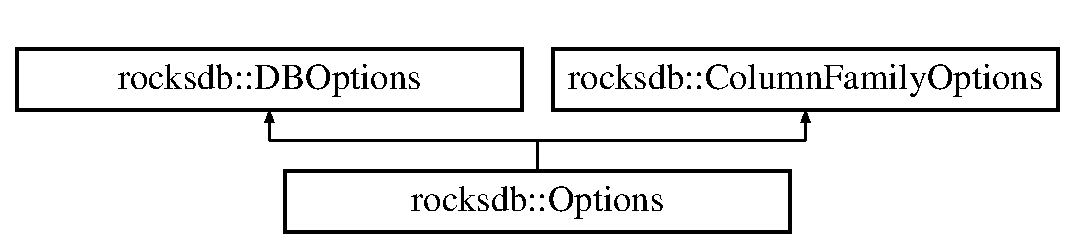
\includegraphics[height=2.000000cm]{structrocksdb_1_1Options}
\end{center}
\end{figure}
\subsection*{Public Member Functions}
\begin{DoxyCompactItemize}
\item 
{\bfseries Options} (const \hyperlink{structrocksdb_1_1DBOptions}{D\+B\+Options} \&db\+\_\+options, const \hyperlink{structrocksdb_1_1ColumnFamilyOptions}{Column\+Family\+Options} \&column\+\_\+family\+\_\+options)\hypertarget{structrocksdb_1_1Options_a7935754a013c35598bc8d20161930263}{}\label{structrocksdb_1_1Options_a7935754a013c35598bc8d20161930263}

\item 
\hyperlink{structrocksdb_1_1Options}{Options} $\ast$ {\bfseries Old\+Defaults} (int rocksdb\+\_\+major\+\_\+version=4, int rocksdb\+\_\+minor\+\_\+version=6)\hypertarget{structrocksdb_1_1Options_afc43721c517950f4e21881448769431e}{}\label{structrocksdb_1_1Options_afc43721c517950f4e21881448769431e}

\item 
void {\bfseries Dump} (\hyperlink{classrocksdb_1_1Logger}{Logger} $\ast$log) const\hypertarget{structrocksdb_1_1Options_a519e1138b450c270f64ca0f5ae42af9c}{}\label{structrocksdb_1_1Options_a519e1138b450c270f64ca0f5ae42af9c}

\item 
void {\bfseries Dump\+C\+F\+Options} (\hyperlink{classrocksdb_1_1Logger}{Logger} $\ast$log) const\hypertarget{structrocksdb_1_1Options_a4e5e05adf317a6aa7b721a41e09b5a95}{}\label{structrocksdb_1_1Options_a4e5e05adf317a6aa7b721a41e09b5a95}

\item 
\hyperlink{structrocksdb_1_1Options}{Options} $\ast$ {\bfseries Prepare\+For\+Bulk\+Load} ()\hypertarget{structrocksdb_1_1Options_ac0a0acc8e851c5fd7ac5dc9e832e0314}{}\label{structrocksdb_1_1Options_ac0a0acc8e851c5fd7ac5dc9e832e0314}

\end{DoxyCompactItemize}
\subsection*{Additional Inherited Members}


The documentation for this struct was generated from the following file\+:\begin{DoxyCompactItemize}
\item 
Appserver/src/external/rocksdb/options.\+h\end{DoxyCompactItemize}

\hypertarget{classJson_1_1OurCharReader}{}\section{Json\+:\+:Our\+Char\+Reader Class Reference}
\label{classJson_1_1OurCharReader}\index{Json\+::\+Our\+Char\+Reader@{Json\+::\+Our\+Char\+Reader}}
Inheritance diagram for Json\+:\+:Our\+Char\+Reader\+:\begin{figure}[H]
\begin{center}
\leavevmode
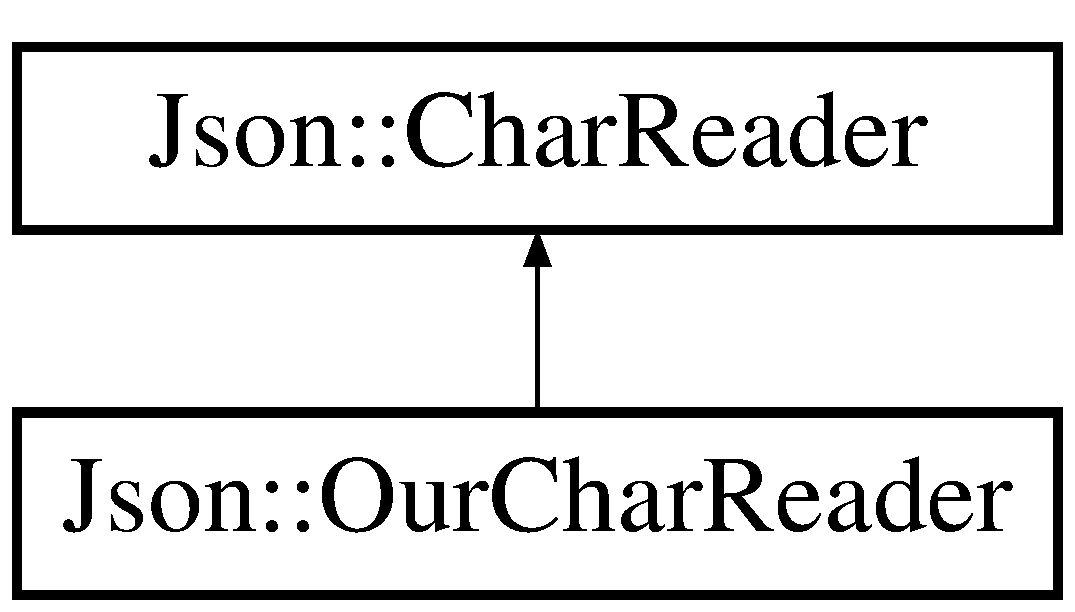
\includegraphics[height=2.000000cm]{classJson_1_1OurCharReader}
\end{center}
\end{figure}
\subsection*{Public Member Functions}
\begin{DoxyCompactItemize}
\item 
{\bfseries Our\+Char\+Reader} (bool collect\+Comments, \hyperlink{classJson_1_1OurFeatures}{Our\+Features} const \&features)\hypertarget{classJson_1_1OurCharReader_a5015506620e7ba7bab417756fa1ca9fe}{}\label{classJson_1_1OurCharReader_a5015506620e7ba7bab417756fa1ca9fe}

\item 
bool \hyperlink{classJson_1_1OurCharReader_a547f08ec5a9951ca69e8bb2e90296c83}{parse} (char const $\ast$begin\+Doc, char const $\ast$end\+Doc, \hyperlink{classJson_1_1Value}{Value} $\ast$root, J\+S\+O\+N\+C\+P\+P\+\_\+\+S\+T\+R\+I\+NG $\ast$errs) J\+S\+O\+N\+C\+P\+P\+\_\+\+O\+V\+E\+R\+R\+I\+DE
\begin{DoxyCompactList}\small\item\em Read a \hyperlink{classJson_1_1Value}{Value} from a \href{http://www.json.org}{\tt J\+S\+ON} document. The document must be a U\+T\+F-\/8 encoded string containing the document to read. \end{DoxyCompactList}\end{DoxyCompactItemize}


\subsection{Member Function Documentation}
\index{Json\+::\+Our\+Char\+Reader@{Json\+::\+Our\+Char\+Reader}!parse@{parse}}
\index{parse@{parse}!Json\+::\+Our\+Char\+Reader@{Json\+::\+Our\+Char\+Reader}}
\subsubsection[{\texorpdfstring{parse(char const $\ast$begin\+Doc, char const $\ast$end\+Doc, Value $\ast$root, J\+S\+O\+N\+C\+P\+P\+\_\+\+S\+T\+R\+I\+N\+G $\ast$errs) J\+S\+O\+N\+C\+P\+P\+\_\+\+O\+V\+E\+R\+R\+I\+DE}{parse(char const *beginDoc, char const *endDoc, Value *root, JSONCPP\_STRING *errs) JSONCPP\_OVERRIDE}}]{\setlength{\rightskip}{0pt plus 5cm}bool Json\+::\+Our\+Char\+Reader\+::parse (
\begin{DoxyParamCaption}
\item[{char const $\ast$}]{begin\+Doc, }
\item[{char const $\ast$}]{end\+Doc, }
\item[{{\bf Value} $\ast$}]{root, }
\item[{J\+S\+O\+N\+C\+P\+P\+\_\+\+S\+T\+R\+I\+NG $\ast$}]{errs}
\end{DoxyParamCaption}
)\hspace{0.3cm}{\ttfamily [inline]}, {\ttfamily [virtual]}}\hypertarget{classJson_1_1OurCharReader_a547f08ec5a9951ca69e8bb2e90296c83}{}\label{classJson_1_1OurCharReader_a547f08ec5a9951ca69e8bb2e90296c83}


Read a \hyperlink{classJson_1_1Value}{Value} from a \href{http://www.json.org}{\tt J\+S\+ON} document. The document must be a U\+T\+F-\/8 encoded string containing the document to read. 


\begin{DoxyParams}{Parameters}
{\em begin\+Doc} & Pointer on the beginning of the U\+T\+F-\/8 encoded string of the document to read. \\
\hline
{\em end\+Doc} & Pointer on the end of the U\+T\+F-\/8 encoded string of the document to read. Must be $>$= begin\+Doc. \\
\hline
{\em root} & \mbox{[}out\mbox{]} Contains the root value of the document if it was successfully parsed. \\
\hline
{\em errs} & \mbox{[}out\mbox{]} Formatted error messages (if not N\+U\+LL) a user friendly string that lists errors in the parsed document. \\
\hline
\end{DoxyParams}
\begin{DoxyReturn}{Returns}
{\ttfamily true} if the document was successfully parsed, {\ttfamily false} if an error occurred. 
\end{DoxyReturn}


Implements \hyperlink{classJson_1_1CharReader_a7983680d50fd0745f371c43b162e78e1}{Json\+::\+Char\+Reader}.



The documentation for this class was generated from the following file\+:\begin{DoxyCompactItemize}
\item 
Appserver/src/external/json/jsoncpp.\+cpp\end{DoxyCompactItemize}

\hypertarget{classJson_1_1OurFeatures}{}\section{Json\+:\+:Our\+Features Class Reference}
\label{classJson_1_1OurFeatures}\index{Json\+::\+Our\+Features@{Json\+::\+Our\+Features}}
\subsection*{Static Public Member Functions}
\begin{DoxyCompactItemize}
\item 
static \hyperlink{classJson_1_1OurFeatures}{Our\+Features} {\bfseries all} ()\hypertarget{classJson_1_1OurFeatures_a0686e1406b6677f496529f9f3fe98d1e}{}\label{classJson_1_1OurFeatures_a0686e1406b6677f496529f9f3fe98d1e}

\end{DoxyCompactItemize}
\subsection*{Public Attributes}
\begin{DoxyCompactItemize}
\item 
bool {\bfseries allow\+Comments\+\_\+}\hypertarget{classJson_1_1OurFeatures_ac71bb7ba7363d3b05ed76602b036ce33}{}\label{classJson_1_1OurFeatures_ac71bb7ba7363d3b05ed76602b036ce33}

\item 
bool {\bfseries strict\+Root\+\_\+}\hypertarget{classJson_1_1OurFeatures_a2095f66a776c0a4ae6cc931a0c94242e}{}\label{classJson_1_1OurFeatures_a2095f66a776c0a4ae6cc931a0c94242e}

\item 
bool {\bfseries allow\+Dropped\+Null\+Placeholders\+\_\+}\hypertarget{classJson_1_1OurFeatures_a13963bc44bf948eec1968f7ff8e8f5f1}{}\label{classJson_1_1OurFeatures_a13963bc44bf948eec1968f7ff8e8f5f1}

\item 
bool {\bfseries allow\+Numeric\+Keys\+\_\+}\hypertarget{classJson_1_1OurFeatures_af6973fc7e774ce2d634ba99442aeb91a}{}\label{classJson_1_1OurFeatures_af6973fc7e774ce2d634ba99442aeb91a}

\item 
bool {\bfseries allow\+Single\+Quotes\+\_\+}\hypertarget{classJson_1_1OurFeatures_abbd6c196d7a22e2a360a59887eda4610}{}\label{classJson_1_1OurFeatures_abbd6c196d7a22e2a360a59887eda4610}

\item 
bool {\bfseries fail\+If\+Extra\+\_\+}\hypertarget{classJson_1_1OurFeatures_ae8ad25b90706c78f1a8fe929191ac61b}{}\label{classJson_1_1OurFeatures_ae8ad25b90706c78f1a8fe929191ac61b}

\item 
bool {\bfseries reject\+Dup\+Keys\+\_\+}\hypertarget{classJson_1_1OurFeatures_a39b8e0b86b1c24a45e800c023bb715aa}{}\label{classJson_1_1OurFeatures_a39b8e0b86b1c24a45e800c023bb715aa}

\item 
bool {\bfseries allow\+Special\+Floats\+\_\+}\hypertarget{classJson_1_1OurFeatures_af760f91cc2a7af37e44f78fb466061bb}{}\label{classJson_1_1OurFeatures_af760f91cc2a7af37e44f78fb466061bb}

\item 
int {\bfseries stack\+Limit\+\_\+}\hypertarget{classJson_1_1OurFeatures_a9a786713902d14be6d57a08cc03ccfff}{}\label{classJson_1_1OurFeatures_a9a786713902d14be6d57a08cc03ccfff}

\end{DoxyCompactItemize}


The documentation for this class was generated from the following file\+:\begin{DoxyCompactItemize}
\item 
Appserver/src/external/json/jsoncpp.\+cpp\end{DoxyCompactItemize}

\hypertarget{classJson_1_1OurReader}{}\section{Json\+:\+:Our\+Reader Class Reference}
\label{classJson_1_1OurReader}\index{Json\+::\+Our\+Reader@{Json\+::\+Our\+Reader}}
\subsection*{Classes}
\begin{DoxyCompactItemize}
\item 
struct \hyperlink{structJson_1_1OurReader_1_1StructuredError}{Structured\+Error}
\end{DoxyCompactItemize}
\subsection*{Public Types}
\begin{DoxyCompactItemize}
\item 
typedef char {\bfseries Char}\hypertarget{classJson_1_1OurReader_a0cd0bab4caa66594ab843ccd5f9dc239}{}\label{classJson_1_1OurReader_a0cd0bab4caa66594ab843ccd5f9dc239}

\item 
typedef const Char $\ast$ {\bfseries Location}\hypertarget{classJson_1_1OurReader_a1bdc7bbc52ba87cae6b19746f2ee0189}{}\label{classJson_1_1OurReader_a1bdc7bbc52ba87cae6b19746f2ee0189}

\end{DoxyCompactItemize}
\subsection*{Public Member Functions}
\begin{DoxyCompactItemize}
\item 
{\bfseries Our\+Reader} (\hyperlink{classJson_1_1OurFeatures}{Our\+Features} const \&features)\hypertarget{classJson_1_1OurReader_a48a850914b9c8d7781be172930c478e5}{}\label{classJson_1_1OurReader_a48a850914b9c8d7781be172930c478e5}

\item 
bool {\bfseries parse} (const char $\ast$begin\+Doc, const char $\ast$end\+Doc, \hyperlink{classJson_1_1Value}{Value} \&root, bool collect\+Comments=true)\hypertarget{classJson_1_1OurReader_aba4f8749aab7f02ec17f107e392caf80}{}\label{classJson_1_1OurReader_aba4f8749aab7f02ec17f107e392caf80}

\item 
J\+S\+O\+N\+C\+P\+P\+\_\+\+S\+T\+R\+I\+NG {\bfseries get\+Formatted\+Error\+Messages} () const\hypertarget{classJson_1_1OurReader_a7971de51d73bb4aee5b0c4742c4aaaac}{}\label{classJson_1_1OurReader_a7971de51d73bb4aee5b0c4742c4aaaac}

\item 
std\+::vector$<$ \hyperlink{structJson_1_1OurReader_1_1StructuredError}{Structured\+Error} $>$ {\bfseries get\+Structured\+Errors} () const\hypertarget{classJson_1_1OurReader_a0eb2420a6bef89a3f3256191e6e3de6d}{}\label{classJson_1_1OurReader_a0eb2420a6bef89a3f3256191e6e3de6d}

\item 
bool {\bfseries push\+Error} (const \hyperlink{classJson_1_1Value}{Value} \&value, const J\+S\+O\+N\+C\+P\+P\+\_\+\+S\+T\+R\+I\+NG \&message)\hypertarget{classJson_1_1OurReader_a700e9d8e0977fa7e0375d26690d7025f}{}\label{classJson_1_1OurReader_a700e9d8e0977fa7e0375d26690d7025f}

\item 
bool {\bfseries push\+Error} (const \hyperlink{classJson_1_1Value}{Value} \&value, const J\+S\+O\+N\+C\+P\+P\+\_\+\+S\+T\+R\+I\+NG \&message, const \hyperlink{classJson_1_1Value}{Value} \&extra)\hypertarget{classJson_1_1OurReader_addccecfca74b79adaad6115ddd614477}{}\label{classJson_1_1OurReader_addccecfca74b79adaad6115ddd614477}

\item 
bool {\bfseries good} () const\hypertarget{classJson_1_1OurReader_a63c7d874fa379397e0a5fa65f0843845}{}\label{classJson_1_1OurReader_a63c7d874fa379397e0a5fa65f0843845}

\end{DoxyCompactItemize}


The documentation for this class was generated from the following file\+:\begin{DoxyCompactItemize}
\item 
Appserver/src/external/json/jsoncpp.\+cpp\end{DoxyCompactItemize}

\hypertarget{classPareja}{}\section{Pareja Class Reference}
\label{classPareja}\index{Pareja@{Pareja}}
\subsection*{Public Member Functions}
\begin{DoxyCompactItemize}
\item 
{\bfseries Pareja} (string usuario1, string usuario2)\hypertarget{classPareja_a4e91ba500129e03a22ca5146d03bd7da}{}\label{classPareja_a4e91ba500129e03a22ca5146d03bd7da}

\item 
{\bfseries Pareja} (string texto)\hypertarget{classPareja_a237161a5d6ce6c3068e4005f33c1ee94}{}\label{classPareja_a237161a5d6ce6c3068e4005f33c1ee94}

\item 
void {\bfseries usuario\+Vota} (string usuario, bool voto\+A\+Favor)\hypertarget{classPareja_a9faf806fe2495b4136e14b6b0880c590}{}\label{classPareja_a9faf806fe2495b4136e14b6b0880c590}

\item 
void {\bfseries notificar\+Usuario} (string usuario)\hypertarget{classPareja_a33774363ab6d6a494b0a6ae0aeafc55a}{}\label{classPareja_a33774363ab6d6a494b0a6ae0aeafc55a}

\item 
bool {\bfseries esta\+Notificado} (string usuario)\hypertarget{classPareja_a008252b44151f929af766c2f896eb6b6}{}\label{classPareja_a008252b44151f929af766c2f896eb6b6}

\item 
bool {\bfseries esta\+Definida} ()\hypertarget{classPareja_a8de1cfa63b2c6e9ee7cacf06945b5e74}{}\label{classPareja_a8de1cfa63b2c6e9ee7cacf06945b5e74}

\item 
bool {\bfseries hay\+Match} ()\hypertarget{classPareja_a1047f97768abe63fdd98e523b859c3a8}{}\label{classPareja_a1047f97768abe63fdd98e523b859c3a8}

\item 
string {\bfseries to\+String} ()\hypertarget{classPareja_a011462c96fb97f4376196b073d141703}{}\label{classPareja_a011462c96fb97f4376196b073d141703}

\end{DoxyCompactItemize}


The documentation for this class was generated from the following files\+:\begin{DoxyCompactItemize}
\item 
Appserver/src/servicios/Pareja.\+h\item 
Appserver/src/servicios/Pareja.\+cpp\end{DoxyCompactItemize}

\hypertarget{classJson_1_1Path}{}\section{Json\+:\+:Path Class Reference}
\label{classJson_1_1Path}\index{Json\+::\+Path@{Json\+::\+Path}}


Experimental and untested\+: represents a \char`\"{}path\char`\"{} to access a node.  




{\ttfamily \#include $<$json.\+h$>$}

\subsection*{Public Member Functions}
\begin{DoxyCompactItemize}
\item 
{\bfseries Path} (const J\+S\+O\+N\+C\+P\+P\+\_\+\+S\+T\+R\+I\+NG \&path, const \hyperlink{classJson_1_1PathArgument}{Path\+Argument} \&a1=\hyperlink{classJson_1_1PathArgument}{Path\+Argument}(), const \hyperlink{classJson_1_1PathArgument}{Path\+Argument} \&a2=\hyperlink{classJson_1_1PathArgument}{Path\+Argument}(), const \hyperlink{classJson_1_1PathArgument}{Path\+Argument} \&a3=\hyperlink{classJson_1_1PathArgument}{Path\+Argument}(), const \hyperlink{classJson_1_1PathArgument}{Path\+Argument} \&a4=\hyperlink{classJson_1_1PathArgument}{Path\+Argument}(), const \hyperlink{classJson_1_1PathArgument}{Path\+Argument} \&a5=\hyperlink{classJson_1_1PathArgument}{Path\+Argument}())\hypertarget{classJson_1_1Path_a7356c0e9c1fc2276390fd396271c1300}{}\label{classJson_1_1Path_a7356c0e9c1fc2276390fd396271c1300}

\item 
const \hyperlink{classJson_1_1Value}{Value} \& {\bfseries resolve} (const \hyperlink{classJson_1_1Value}{Value} \&root) const\hypertarget{classJson_1_1Path_ad1abdc54d2e03fc0e9436c3b9fd55a33}{}\label{classJson_1_1Path_ad1abdc54d2e03fc0e9436c3b9fd55a33}

\item 
\hyperlink{classJson_1_1Value}{Value} {\bfseries resolve} (const \hyperlink{classJson_1_1Value}{Value} \&root, const \hyperlink{classJson_1_1Value}{Value} \&default\+Value) const\hypertarget{classJson_1_1Path_ab65ab001ccdbc6f8b5f123da58b92539}{}\label{classJson_1_1Path_ab65ab001ccdbc6f8b5f123da58b92539}

\item 
\hyperlink{classJson_1_1Value}{Value} \& \hyperlink{classJson_1_1Path_a858f9426f0f7bbe0450644d72b44e26b}{make} (\hyperlink{classJson_1_1Value}{Value} \&root) const
\end{DoxyCompactItemize}


\subsection{Detailed Description}
Experimental and untested\+: represents a \char`\"{}path\char`\"{} to access a node. 

Syntax\+:
\begin{DoxyItemize}
\item \char`\"{}.\char`\"{} =$>$ root node
\item \char`\"{}.\mbox{[}n\mbox{]}\char`\"{} =$>$ elements at index \textquotesingle{}n\textquotesingle{} of root node (an array value)
\item \char`\"{}.\+name\char`\"{} =$>$ member named \textquotesingle{}name\textquotesingle{} of root node (an object value)
\item \char`\"{}.\+name1.\+name2.\+name3\char`\"{}
\item \char`\"{}.\mbox{[}0\mbox{]}\mbox{[}1\mbox{]}\mbox{[}2\mbox{]}.\+name1\mbox{[}3\mbox{]}\char`\"{}
\item \char`\"{}.\%\char`\"{} =$>$ member name is provided as parameter
\item \char`\"{}.\mbox{[}\%\mbox{]}\char`\"{} =$>$ index is provied as parameter 
\end{DoxyItemize}

\subsection{Member Function Documentation}
\index{Json\+::\+Path@{Json\+::\+Path}!make@{make}}
\index{make@{make}!Json\+::\+Path@{Json\+::\+Path}}
\subsubsection[{\texorpdfstring{make(\+Value \&root) const}{make(Value \&root) const}}]{\setlength{\rightskip}{0pt plus 5cm}{\bf Value} \& Json\+::\+Path\+::make (
\begin{DoxyParamCaption}
\item[{{\bf Value} \&}]{root}
\end{DoxyParamCaption}
) const}\hypertarget{classJson_1_1Path_a858f9426f0f7bbe0450644d72b44e26b}{}\label{classJson_1_1Path_a858f9426f0f7bbe0450644d72b44e26b}
Creates the \char`\"{}path\char`\"{} to access the specified node and returns a reference on the node. 

The documentation for this class was generated from the following files\+:\begin{DoxyCompactItemize}
\item 
Appserver/src/external/json/json.\+h\item 
Appserver/src/external/json/jsoncpp.\+cpp\end{DoxyCompactItemize}

\hypertarget{classJson_1_1PathArgument}{}\section{Json\+:\+:Path\+Argument Class Reference}
\label{classJson_1_1PathArgument}\index{Json\+::\+Path\+Argument@{Json\+::\+Path\+Argument}}


Experimental and untested\+: represents an element of the \char`\"{}path\char`\"{} to access a node.  




{\ttfamily \#include $<$json.\+h$>$}

\subsection*{Public Member Functions}
\begin{DoxyCompactItemize}
\item 
{\bfseries Path\+Argument} (Array\+Index index)\hypertarget{classJson_1_1PathArgument_a53c5b27143b161301b95fd544c139ecf}{}\label{classJson_1_1PathArgument_a53c5b27143b161301b95fd544c139ecf}

\item 
{\bfseries Path\+Argument} (const char $\ast$key)\hypertarget{classJson_1_1PathArgument_a9690417a8a40e6e49f2acdf6c9281345}{}\label{classJson_1_1PathArgument_a9690417a8a40e6e49f2acdf6c9281345}

\item 
{\bfseries Path\+Argument} (const J\+S\+O\+N\+C\+P\+P\+\_\+\+S\+T\+R\+I\+NG \&key)\hypertarget{classJson_1_1PathArgument_ac15f25452124fbf21218897113015301}{}\label{classJson_1_1PathArgument_ac15f25452124fbf21218897113015301}

\end{DoxyCompactItemize}
\subsection*{Friends}
\begin{DoxyCompactItemize}
\item 
class {\bfseries Path}\hypertarget{classJson_1_1PathArgument_a4877239a6b7f09fbf5a61ca68a49d74c}{}\label{classJson_1_1PathArgument_a4877239a6b7f09fbf5a61ca68a49d74c}

\end{DoxyCompactItemize}


\subsection{Detailed Description}
Experimental and untested\+: represents an element of the \char`\"{}path\char`\"{} to access a node. 

The documentation for this class was generated from the following files\+:\begin{DoxyCompactItemize}
\item 
Appserver/src/external/json/json.\+h\item 
Appserver/src/external/json/jsoncpp.\+cpp\end{DoxyCompactItemize}

\hypertarget{structrocksdb_1_1PerfContext}{}\section{rocksdb\+:\+:Perf\+Context Struct Reference}
\label{structrocksdb_1_1PerfContext}\index{rocksdb\+::\+Perf\+Context@{rocksdb\+::\+Perf\+Context}}
\subsection*{Public Member Functions}
\begin{DoxyCompactItemize}
\item 
void {\bfseries Reset} ()\hypertarget{structrocksdb_1_1PerfContext_ac2c04bd14e4d8f51335e93aaeb10f7d2}{}\label{structrocksdb_1_1PerfContext_ac2c04bd14e4d8f51335e93aaeb10f7d2}

\item 
std\+::string {\bfseries To\+String} (bool exclude\+\_\+zero\+\_\+counters=false) const\hypertarget{structrocksdb_1_1PerfContext_aea9da9ad9fc08a0f8e7776e96aed19b8}{}\label{structrocksdb_1_1PerfContext_aea9da9ad9fc08a0f8e7776e96aed19b8}

\end{DoxyCompactItemize}
\subsection*{Public Attributes}
\begin{DoxyCompactItemize}
\item 
uint64\+\_\+t {\bfseries user\+\_\+key\+\_\+comparison\+\_\+count}\hypertarget{structrocksdb_1_1PerfContext_ae90efece24dca3684c77262c575247b7}{}\label{structrocksdb_1_1PerfContext_ae90efece24dca3684c77262c575247b7}

\item 
uint64\+\_\+t {\bfseries block\+\_\+cache\+\_\+hit\+\_\+count}\hypertarget{structrocksdb_1_1PerfContext_a034813413724e824371c191f596ed02c}{}\label{structrocksdb_1_1PerfContext_a034813413724e824371c191f596ed02c}

\item 
uint64\+\_\+t {\bfseries block\+\_\+read\+\_\+count}\hypertarget{structrocksdb_1_1PerfContext_ace0c47e3acad250bfb7c815a7963e912}{}\label{structrocksdb_1_1PerfContext_ace0c47e3acad250bfb7c815a7963e912}

\item 
uint64\+\_\+t {\bfseries block\+\_\+read\+\_\+byte}\hypertarget{structrocksdb_1_1PerfContext_afb97c7bc14d7b1ca74b60b61e418c32a}{}\label{structrocksdb_1_1PerfContext_afb97c7bc14d7b1ca74b60b61e418c32a}

\item 
uint64\+\_\+t {\bfseries block\+\_\+read\+\_\+time}\hypertarget{structrocksdb_1_1PerfContext_a872ba73b4df2b9d58723dca18ba8b9b7}{}\label{structrocksdb_1_1PerfContext_a872ba73b4df2b9d58723dca18ba8b9b7}

\item 
uint64\+\_\+t {\bfseries block\+\_\+checksum\+\_\+time}\hypertarget{structrocksdb_1_1PerfContext_a419d3b4d1b8fa64d5ccee3c66def1fc5}{}\label{structrocksdb_1_1PerfContext_a419d3b4d1b8fa64d5ccee3c66def1fc5}

\item 
uint64\+\_\+t {\bfseries block\+\_\+decompress\+\_\+time}\hypertarget{structrocksdb_1_1PerfContext_a2a522aa62c94e93327ce8361c0d77b58}{}\label{structrocksdb_1_1PerfContext_a2a522aa62c94e93327ce8361c0d77b58}

\item 
uint64\+\_\+t {\bfseries internal\+\_\+key\+\_\+skipped\+\_\+count}\hypertarget{structrocksdb_1_1PerfContext_a849a7efb6bce5d1d675db89852881a6c}{}\label{structrocksdb_1_1PerfContext_a849a7efb6bce5d1d675db89852881a6c}

\item 
uint64\+\_\+t {\bfseries internal\+\_\+delete\+\_\+skipped\+\_\+count}\hypertarget{structrocksdb_1_1PerfContext_a2fb2fc7ca3d03c11ae41495ed05aeca0}{}\label{structrocksdb_1_1PerfContext_a2fb2fc7ca3d03c11ae41495ed05aeca0}

\item 
uint64\+\_\+t {\bfseries get\+\_\+snapshot\+\_\+time}\hypertarget{structrocksdb_1_1PerfContext_a466bf412e99135ec86e99bb1fbb7fbd5}{}\label{structrocksdb_1_1PerfContext_a466bf412e99135ec86e99bb1fbb7fbd5}

\item 
uint64\+\_\+t {\bfseries get\+\_\+from\+\_\+memtable\+\_\+time}\hypertarget{structrocksdb_1_1PerfContext_aa46317faa0db735d6e7bec7e32ce38b0}{}\label{structrocksdb_1_1PerfContext_aa46317faa0db735d6e7bec7e32ce38b0}

\item 
uint64\+\_\+t {\bfseries get\+\_\+from\+\_\+memtable\+\_\+count}\hypertarget{structrocksdb_1_1PerfContext_a1387053c83069f69706effa9560d577a}{}\label{structrocksdb_1_1PerfContext_a1387053c83069f69706effa9560d577a}

\item 
uint64\+\_\+t {\bfseries get\+\_\+post\+\_\+process\+\_\+time}\hypertarget{structrocksdb_1_1PerfContext_a025fc69f40feaae5e96adc7dc9613b19}{}\label{structrocksdb_1_1PerfContext_a025fc69f40feaae5e96adc7dc9613b19}

\item 
uint64\+\_\+t {\bfseries get\+\_\+from\+\_\+output\+\_\+files\+\_\+time}\hypertarget{structrocksdb_1_1PerfContext_a62538356efc1db3333e8e6d4336b66b1}{}\label{structrocksdb_1_1PerfContext_a62538356efc1db3333e8e6d4336b66b1}

\item 
uint64\+\_\+t {\bfseries seek\+\_\+on\+\_\+memtable\+\_\+time}\hypertarget{structrocksdb_1_1PerfContext_ace6f919b87b4ede0ed247f6aaa74492e}{}\label{structrocksdb_1_1PerfContext_ace6f919b87b4ede0ed247f6aaa74492e}

\item 
uint64\+\_\+t {\bfseries seek\+\_\+on\+\_\+memtable\+\_\+count}\hypertarget{structrocksdb_1_1PerfContext_a6155b2dd6b5c36c72d71243c55e50a62}{}\label{structrocksdb_1_1PerfContext_a6155b2dd6b5c36c72d71243c55e50a62}

\item 
uint64\+\_\+t {\bfseries seek\+\_\+child\+\_\+seek\+\_\+time}\hypertarget{structrocksdb_1_1PerfContext_ae67ca2cecc9a04505d67c3138dd2378b}{}\label{structrocksdb_1_1PerfContext_ae67ca2cecc9a04505d67c3138dd2378b}

\item 
uint64\+\_\+t {\bfseries seek\+\_\+child\+\_\+seek\+\_\+count}\hypertarget{structrocksdb_1_1PerfContext_ad7740027368daaeb0fb9aead7da8fda4}{}\label{structrocksdb_1_1PerfContext_ad7740027368daaeb0fb9aead7da8fda4}

\item 
uint64\+\_\+t {\bfseries seek\+\_\+min\+\_\+heap\+\_\+time}\hypertarget{structrocksdb_1_1PerfContext_a6b9307813ea5cb2c7b113004ef71fd9e}{}\label{structrocksdb_1_1PerfContext_a6b9307813ea5cb2c7b113004ef71fd9e}

\item 
uint64\+\_\+t {\bfseries seek\+\_\+internal\+\_\+seek\+\_\+time}\hypertarget{structrocksdb_1_1PerfContext_a12783c96b370ceadf215c51765f792d1}{}\label{structrocksdb_1_1PerfContext_a12783c96b370ceadf215c51765f792d1}

\item 
uint64\+\_\+t {\bfseries find\+\_\+next\+\_\+user\+\_\+entry\+\_\+time}\hypertarget{structrocksdb_1_1PerfContext_a04a41f137d51d069f63918278010fc17}{}\label{structrocksdb_1_1PerfContext_a04a41f137d51d069f63918278010fc17}

\item 
uint64\+\_\+t {\bfseries write\+\_\+wal\+\_\+time}\hypertarget{structrocksdb_1_1PerfContext_a642c74d50a90f89fcf602ae03701dc17}{}\label{structrocksdb_1_1PerfContext_a642c74d50a90f89fcf602ae03701dc17}

\item 
uint64\+\_\+t {\bfseries write\+\_\+memtable\+\_\+time}\hypertarget{structrocksdb_1_1PerfContext_a6a8fbf490591369c99dd8b2007cc5c56}{}\label{structrocksdb_1_1PerfContext_a6a8fbf490591369c99dd8b2007cc5c56}

\item 
uint64\+\_\+t {\bfseries write\+\_\+delay\+\_\+time}\hypertarget{structrocksdb_1_1PerfContext_a0b4ec7be0221811768938460590c352c}{}\label{structrocksdb_1_1PerfContext_a0b4ec7be0221811768938460590c352c}

\item 
uint64\+\_\+t {\bfseries write\+\_\+pre\+\_\+and\+\_\+post\+\_\+process\+\_\+time}\hypertarget{structrocksdb_1_1PerfContext_a7ab63f68d710cbf8c8667e6e42d8c6f2}{}\label{structrocksdb_1_1PerfContext_a7ab63f68d710cbf8c8667e6e42d8c6f2}

\item 
uint64\+\_\+t {\bfseries db\+\_\+mutex\+\_\+lock\+\_\+nanos}\hypertarget{structrocksdb_1_1PerfContext_afbc9e4025fe20328a649b4021fd6be9a}{}\label{structrocksdb_1_1PerfContext_afbc9e4025fe20328a649b4021fd6be9a}

\item 
uint64\+\_\+t {\bfseries db\+\_\+condition\+\_\+wait\+\_\+nanos}\hypertarget{structrocksdb_1_1PerfContext_a9aeeadf4d92814db27029d7fc286bbf3}{}\label{structrocksdb_1_1PerfContext_a9aeeadf4d92814db27029d7fc286bbf3}

\item 
uint64\+\_\+t {\bfseries merge\+\_\+operator\+\_\+time\+\_\+nanos}\hypertarget{structrocksdb_1_1PerfContext_a7d333a7cab3671db5786486012e55d89}{}\label{structrocksdb_1_1PerfContext_a7d333a7cab3671db5786486012e55d89}

\item 
uint64\+\_\+t {\bfseries read\+\_\+index\+\_\+block\+\_\+nanos}\hypertarget{structrocksdb_1_1PerfContext_a925ecb2f530771d3c790c48ff03f688a}{}\label{structrocksdb_1_1PerfContext_a925ecb2f530771d3c790c48ff03f688a}

\item 
uint64\+\_\+t {\bfseries read\+\_\+filter\+\_\+block\+\_\+nanos}\hypertarget{structrocksdb_1_1PerfContext_a006f2af75c1f5c885f6d2a49138e9ff4}{}\label{structrocksdb_1_1PerfContext_a006f2af75c1f5c885f6d2a49138e9ff4}

\item 
uint64\+\_\+t {\bfseries new\+\_\+table\+\_\+block\+\_\+iter\+\_\+nanos}\hypertarget{structrocksdb_1_1PerfContext_aebeb9767a08f31fa186e6863dce24b42}{}\label{structrocksdb_1_1PerfContext_aebeb9767a08f31fa186e6863dce24b42}

\item 
uint64\+\_\+t {\bfseries new\+\_\+table\+\_\+iterator\+\_\+nanos}\hypertarget{structrocksdb_1_1PerfContext_afdceee4da0e33cea292483d113ed1b9e}{}\label{structrocksdb_1_1PerfContext_afdceee4da0e33cea292483d113ed1b9e}

\item 
uint64\+\_\+t {\bfseries block\+\_\+seek\+\_\+nanos}\hypertarget{structrocksdb_1_1PerfContext_aaddbc7a2cf8ae3412f3707fe56eb6975}{}\label{structrocksdb_1_1PerfContext_aaddbc7a2cf8ae3412f3707fe56eb6975}

\item 
uint64\+\_\+t {\bfseries find\+\_\+table\+\_\+nanos}\hypertarget{structrocksdb_1_1PerfContext_a4da00a42691d3d9a2133d9282f90824b}{}\label{structrocksdb_1_1PerfContext_a4da00a42691d3d9a2133d9282f90824b}

\item 
uint64\+\_\+t {\bfseries bloom\+\_\+memtable\+\_\+hit\+\_\+count}\hypertarget{structrocksdb_1_1PerfContext_ab7657b11760b345e607809fb9b68ae7d}{}\label{structrocksdb_1_1PerfContext_ab7657b11760b345e607809fb9b68ae7d}

\item 
uint64\+\_\+t {\bfseries bloom\+\_\+memtable\+\_\+miss\+\_\+count}\hypertarget{structrocksdb_1_1PerfContext_affe4959eb50abb55ce766ac4a668194d}{}\label{structrocksdb_1_1PerfContext_affe4959eb50abb55ce766ac4a668194d}

\item 
uint64\+\_\+t {\bfseries bloom\+\_\+sst\+\_\+hit\+\_\+count}\hypertarget{structrocksdb_1_1PerfContext_a73c0208deb4a468ce25ea95e38f5f8f5}{}\label{structrocksdb_1_1PerfContext_a73c0208deb4a468ce25ea95e38f5f8f5}

\item 
uint64\+\_\+t {\bfseries bloom\+\_\+sst\+\_\+miss\+\_\+count}\hypertarget{structrocksdb_1_1PerfContext_a98783a9f14db46800a71881d777c024b}{}\label{structrocksdb_1_1PerfContext_a98783a9f14db46800a71881d777c024b}

\end{DoxyCompactItemize}


The documentation for this struct was generated from the following file\+:\begin{DoxyCompactItemize}
\item 
Appserver/src/external/rocksdb/perf\+\_\+context.\+h\end{DoxyCompactItemize}

\hypertarget{structrocksdb_1_1PlainTableOptions}{}\section{rocksdb\+:\+:Plain\+Table\+Options Struct Reference}
\label{structrocksdb_1_1PlainTableOptions}\index{rocksdb\+::\+Plain\+Table\+Options@{rocksdb\+::\+Plain\+Table\+Options}}
\subsection*{Public Attributes}
\begin{DoxyCompactItemize}
\item 
uint32\+\_\+t {\bfseries user\+\_\+key\+\_\+len} = k\+Plain\+Table\+Variable\+Length\hypertarget{structrocksdb_1_1PlainTableOptions_a6d033f071f8843eccd43457bb69863de}{}\label{structrocksdb_1_1PlainTableOptions_a6d033f071f8843eccd43457bb69863de}

\item 
int {\bfseries bloom\+\_\+bits\+\_\+per\+\_\+key} = 10\hypertarget{structrocksdb_1_1PlainTableOptions_a3eee69ca32c8046d65b2072e78adae5c}{}\label{structrocksdb_1_1PlainTableOptions_a3eee69ca32c8046d65b2072e78adae5c}

\item 
double {\bfseries hash\+\_\+table\+\_\+ratio} = 0.\+75\hypertarget{structrocksdb_1_1PlainTableOptions_ad7ba4c41f318b6df711a9b3b99982d35}{}\label{structrocksdb_1_1PlainTableOptions_ad7ba4c41f318b6df711a9b3b99982d35}

\item 
size\+\_\+t {\bfseries index\+\_\+sparseness} = 16\hypertarget{structrocksdb_1_1PlainTableOptions_ac6cedd6bf5bd2c707bd1ebb11958ddc5}{}\label{structrocksdb_1_1PlainTableOptions_ac6cedd6bf5bd2c707bd1ebb11958ddc5}

\item 
size\+\_\+t {\bfseries huge\+\_\+page\+\_\+tlb\+\_\+size} = 0\hypertarget{structrocksdb_1_1PlainTableOptions_add296e65ac19217093b85f3f6df0c380}{}\label{structrocksdb_1_1PlainTableOptions_add296e65ac19217093b85f3f6df0c380}

\item 
Encoding\+Type {\bfseries encoding\+\_\+type} = k\+Plain\hypertarget{structrocksdb_1_1PlainTableOptions_a58e84a7af9a0faab3c06c0d4b967afb3}{}\label{structrocksdb_1_1PlainTableOptions_a58e84a7af9a0faab3c06c0d4b967afb3}

\item 
bool {\bfseries full\+\_\+scan\+\_\+mode} = false\hypertarget{structrocksdb_1_1PlainTableOptions_a50f67b78797d2cc231889a403e5b7154}{}\label{structrocksdb_1_1PlainTableOptions_a50f67b78797d2cc231889a403e5b7154}

\item 
bool {\bfseries store\+\_\+index\+\_\+in\+\_\+file} = false\hypertarget{structrocksdb_1_1PlainTableOptions_a1f771cd742a3bbdb9d658db23ac1f90d}{}\label{structrocksdb_1_1PlainTableOptions_a1f771cd742a3bbdb9d658db23ac1f90d}

\end{DoxyCompactItemize}


The documentation for this struct was generated from the following file\+:\begin{DoxyCompactItemize}
\item 
Appserver/src/external/rocksdb/table.\+h\end{DoxyCompactItemize}

\hypertarget{structrocksdb_1_1PlainTablePropertyNames}{}\section{rocksdb\+:\+:Plain\+Table\+Property\+Names Struct Reference}
\label{structrocksdb_1_1PlainTablePropertyNames}\index{rocksdb\+::\+Plain\+Table\+Property\+Names@{rocksdb\+::\+Plain\+Table\+Property\+Names}}
\subsection*{Static Public Attributes}
\begin{DoxyCompactItemize}
\item 
static const std\+::string {\bfseries k\+Prefix\+Extractor\+Name}\hypertarget{structrocksdb_1_1PlainTablePropertyNames_acbb40c6ff38d62747e8cef4bda3f31dd}{}\label{structrocksdb_1_1PlainTablePropertyNames_acbb40c6ff38d62747e8cef4bda3f31dd}

\item 
static const std\+::string {\bfseries k\+Encoding\+Type}\hypertarget{structrocksdb_1_1PlainTablePropertyNames_a1e7c00d6bb3c3ef65693d34ecc49d56a}{}\label{structrocksdb_1_1PlainTablePropertyNames_a1e7c00d6bb3c3ef65693d34ecc49d56a}

\item 
static const std\+::string {\bfseries k\+Bloom\+Version}\hypertarget{structrocksdb_1_1PlainTablePropertyNames_a27959690a128c0b8351e586a4f8de091}{}\label{structrocksdb_1_1PlainTablePropertyNames_a27959690a128c0b8351e586a4f8de091}

\item 
static const std\+::string {\bfseries k\+Num\+Bloom\+Blocks}\hypertarget{structrocksdb_1_1PlainTablePropertyNames_a9165271d283adc7d2a695ad15fdebed9}{}\label{structrocksdb_1_1PlainTablePropertyNames_a9165271d283adc7d2a695ad15fdebed9}

\end{DoxyCompactItemize}


The documentation for this struct was generated from the following file\+:\begin{DoxyCompactItemize}
\item 
Appserver/src/external/rocksdb/table.\+h\end{DoxyCompactItemize}

\hypertarget{structrocksdb_1_1DB_1_1Properties}{}\section{rocksdb\+:\+:DB\+:\+:Properties Struct Reference}
\label{structrocksdb_1_1DB_1_1Properties}\index{rocksdb\+::\+D\+B\+::\+Properties@{rocksdb\+::\+D\+B\+::\+Properties}}
\subsection*{Static Public Attributes}
\begin{DoxyCompactItemize}
\item 
static const std\+::string {\bfseries k\+Num\+Files\+At\+Level\+Prefix}\hypertarget{structrocksdb_1_1DB_1_1Properties_abe653893712dc310cdc5d37afde1404d}{}\label{structrocksdb_1_1DB_1_1Properties_abe653893712dc310cdc5d37afde1404d}

\item 
static const std\+::string {\bfseries k\+Stats}\hypertarget{structrocksdb_1_1DB_1_1Properties_a8d19649d9d1251d214a30643cc950e6e}{}\label{structrocksdb_1_1DB_1_1Properties_a8d19649d9d1251d214a30643cc950e6e}

\item 
static const std\+::string {\bfseries k\+S\+S\+Tables}\hypertarget{structrocksdb_1_1DB_1_1Properties_a4a704e886c572a3016786cc9b9a713a7}{}\label{structrocksdb_1_1DB_1_1Properties_a4a704e886c572a3016786cc9b9a713a7}

\item 
static const std\+::string {\bfseries k\+C\+F\+Stats}\hypertarget{structrocksdb_1_1DB_1_1Properties_a75c576e178fafe9c75c8f16c28562a9b}{}\label{structrocksdb_1_1DB_1_1Properties_a75c576e178fafe9c75c8f16c28562a9b}

\item 
static const std\+::string {\bfseries k\+D\+B\+Stats}\hypertarget{structrocksdb_1_1DB_1_1Properties_ad965d683e36095ed5b3b3143657938f7}{}\label{structrocksdb_1_1DB_1_1Properties_ad965d683e36095ed5b3b3143657938f7}

\item 
static const std\+::string {\bfseries k\+Level\+Stats}\hypertarget{structrocksdb_1_1DB_1_1Properties_a19884b12c9ec61d0a165e01540d8e0a4}{}\label{structrocksdb_1_1DB_1_1Properties_a19884b12c9ec61d0a165e01540d8e0a4}

\item 
static const std\+::string {\bfseries k\+Num\+Immutable\+Mem\+Table}\hypertarget{structrocksdb_1_1DB_1_1Properties_a1170040f6b53207276b78857afb17f73}{}\label{structrocksdb_1_1DB_1_1Properties_a1170040f6b53207276b78857afb17f73}

\item 
static const std\+::string {\bfseries k\+Num\+Immutable\+Mem\+Table\+Flushed}\hypertarget{structrocksdb_1_1DB_1_1Properties_a8d7e638b5e0d14edf1d17465b777193d}{}\label{structrocksdb_1_1DB_1_1Properties_a8d7e638b5e0d14edf1d17465b777193d}

\item 
static const std\+::string {\bfseries k\+Mem\+Table\+Flush\+Pending}\hypertarget{structrocksdb_1_1DB_1_1Properties_a66d17eb32157ef7d7d49aa1f693badfb}{}\label{structrocksdb_1_1DB_1_1Properties_a66d17eb32157ef7d7d49aa1f693badfb}

\item 
static const std\+::string {\bfseries k\+Num\+Running\+Flushes}\hypertarget{structrocksdb_1_1DB_1_1Properties_a96e8694cefc187caec15225d6943159e}{}\label{structrocksdb_1_1DB_1_1Properties_a96e8694cefc187caec15225d6943159e}

\item 
static const std\+::string {\bfseries k\+Compaction\+Pending}\hypertarget{structrocksdb_1_1DB_1_1Properties_a2c2ccdf5371af903899b10596b4e5a1c}{}\label{structrocksdb_1_1DB_1_1Properties_a2c2ccdf5371af903899b10596b4e5a1c}

\item 
static const std\+::string {\bfseries k\+Num\+Running\+Compactions}\hypertarget{structrocksdb_1_1DB_1_1Properties_a3286565eff8439c54b849e603c85fc48}{}\label{structrocksdb_1_1DB_1_1Properties_a3286565eff8439c54b849e603c85fc48}

\item 
static const std\+::string {\bfseries k\+Background\+Errors}\hypertarget{structrocksdb_1_1DB_1_1Properties_af8c84eb10690dd07bbf2e907e11be309}{}\label{structrocksdb_1_1DB_1_1Properties_af8c84eb10690dd07bbf2e907e11be309}

\item 
static const std\+::string {\bfseries k\+Cur\+Size\+Active\+Mem\+Table}\hypertarget{structrocksdb_1_1DB_1_1Properties_a51acf2eefa22032a0a26e8bfcbf3b8fe}{}\label{structrocksdb_1_1DB_1_1Properties_a51acf2eefa22032a0a26e8bfcbf3b8fe}

\item 
static const std\+::string {\bfseries k\+Cur\+Size\+All\+Mem\+Tables}\hypertarget{structrocksdb_1_1DB_1_1Properties_a9a94abbbf98153f8487ec27c9086e1ec}{}\label{structrocksdb_1_1DB_1_1Properties_a9a94abbbf98153f8487ec27c9086e1ec}

\item 
static const std\+::string {\bfseries k\+Size\+All\+Mem\+Tables}\hypertarget{structrocksdb_1_1DB_1_1Properties_a57adbc2205e318f7b1d9f351d896cf1b}{}\label{structrocksdb_1_1DB_1_1Properties_a57adbc2205e318f7b1d9f351d896cf1b}

\item 
static const std\+::string {\bfseries k\+Num\+Entries\+Active\+Mem\+Table}\hypertarget{structrocksdb_1_1DB_1_1Properties_afe59d185c3d4335dca9e76c1fd0e90c7}{}\label{structrocksdb_1_1DB_1_1Properties_afe59d185c3d4335dca9e76c1fd0e90c7}

\item 
static const std\+::string {\bfseries k\+Num\+Entries\+Imm\+Mem\+Tables}\hypertarget{structrocksdb_1_1DB_1_1Properties_a35409c653b07f51c395ba3f5187a08c3}{}\label{structrocksdb_1_1DB_1_1Properties_a35409c653b07f51c395ba3f5187a08c3}

\item 
static const std\+::string {\bfseries k\+Num\+Deletes\+Active\+Mem\+Table}\hypertarget{structrocksdb_1_1DB_1_1Properties_af38d4988f4b80489a0802912ad41ab34}{}\label{structrocksdb_1_1DB_1_1Properties_af38d4988f4b80489a0802912ad41ab34}

\item 
static const std\+::string {\bfseries k\+Num\+Deletes\+Imm\+Mem\+Tables}\hypertarget{structrocksdb_1_1DB_1_1Properties_a80cc468673d702b329023954843997ee}{}\label{structrocksdb_1_1DB_1_1Properties_a80cc468673d702b329023954843997ee}

\item 
static const std\+::string {\bfseries k\+Estimate\+Num\+Keys}\hypertarget{structrocksdb_1_1DB_1_1Properties_af664721657451d1ffdaf95bb1adb9dc4}{}\label{structrocksdb_1_1DB_1_1Properties_af664721657451d1ffdaf95bb1adb9dc4}

\item 
static const std\+::string {\bfseries k\+Estimate\+Table\+Readers\+Mem}\hypertarget{structrocksdb_1_1DB_1_1Properties_a0ce715786886632d11136bafd288ec4a}{}\label{structrocksdb_1_1DB_1_1Properties_a0ce715786886632d11136bafd288ec4a}

\item 
static const std\+::string {\bfseries k\+Is\+File\+Deletions\+Enabled}\hypertarget{structrocksdb_1_1DB_1_1Properties_a5d96a41d246b9c79b237183288e509b2}{}\label{structrocksdb_1_1DB_1_1Properties_a5d96a41d246b9c79b237183288e509b2}

\item 
static const std\+::string {\bfseries k\+Num\+Snapshots}\hypertarget{structrocksdb_1_1DB_1_1Properties_af56f16e223d74e719de1f755f5dfb1c2}{}\label{structrocksdb_1_1DB_1_1Properties_af56f16e223d74e719de1f755f5dfb1c2}

\item 
static const std\+::string {\bfseries k\+Oldest\+Snapshot\+Time}\hypertarget{structrocksdb_1_1DB_1_1Properties_a4485c154f73d9cf915322f2ae12f9506}{}\label{structrocksdb_1_1DB_1_1Properties_a4485c154f73d9cf915322f2ae12f9506}

\item 
static const std\+::string {\bfseries k\+Num\+Live\+Versions}\hypertarget{structrocksdb_1_1DB_1_1Properties_af9bf762044587e07ea3f48f973089a61}{}\label{structrocksdb_1_1DB_1_1Properties_af9bf762044587e07ea3f48f973089a61}

\item 
static const std\+::string {\bfseries k\+Current\+Super\+Version\+Number}\hypertarget{structrocksdb_1_1DB_1_1Properties_a11d95a8c34935217a56ba81daa015b16}{}\label{structrocksdb_1_1DB_1_1Properties_a11d95a8c34935217a56ba81daa015b16}

\item 
static const std\+::string {\bfseries k\+Estimate\+Live\+Data\+Size}\hypertarget{structrocksdb_1_1DB_1_1Properties_a891ba40a43771067adea93591d3bed46}{}\label{structrocksdb_1_1DB_1_1Properties_a891ba40a43771067adea93591d3bed46}

\item 
static const std\+::string {\bfseries k\+Total\+Sst\+Files\+Size}\hypertarget{structrocksdb_1_1DB_1_1Properties_a1754317492b469699a2aec849791aaab}{}\label{structrocksdb_1_1DB_1_1Properties_a1754317492b469699a2aec849791aaab}

\item 
static const std\+::string {\bfseries k\+Base\+Level}\hypertarget{structrocksdb_1_1DB_1_1Properties_a5168fb4704c9615855f00e278bcc4f41}{}\label{structrocksdb_1_1DB_1_1Properties_a5168fb4704c9615855f00e278bcc4f41}

\item 
static const std\+::string {\bfseries k\+Estimate\+Pending\+Compaction\+Bytes}\hypertarget{structrocksdb_1_1DB_1_1Properties_a3e0f31b77f9d37912725af7e1c22b2bf}{}\label{structrocksdb_1_1DB_1_1Properties_a3e0f31b77f9d37912725af7e1c22b2bf}

\item 
static const std\+::string {\bfseries k\+Aggregated\+Table\+Properties}\hypertarget{structrocksdb_1_1DB_1_1Properties_ab431ed4ab2413b32f09a2511fd8d25a7}{}\label{structrocksdb_1_1DB_1_1Properties_ab431ed4ab2413b32f09a2511fd8d25a7}

\item 
static const std\+::string {\bfseries k\+Aggregated\+Table\+Properties\+At\+Level}\hypertarget{structrocksdb_1_1DB_1_1Properties_a851d4c3de94417af2e9a1c0a59716abe}{}\label{structrocksdb_1_1DB_1_1Properties_a851d4c3de94417af2e9a1c0a59716abe}

\end{DoxyCompactItemize}


The documentation for this struct was generated from the following file\+:\begin{DoxyCompactItemize}
\item 
Appserver/src/external/rocksdb/db.\+h\end{DoxyCompactItemize}

\hypertarget{classrocksdb_1_1RandomAccessFile}{}\section{rocksdb\+:\+:Random\+Access\+File Class Reference}
\label{classrocksdb_1_1RandomAccessFile}\index{rocksdb\+::\+Random\+Access\+File@{rocksdb\+::\+Random\+Access\+File}}
\subsection*{Public Types}
\begin{DoxyCompactItemize}
\item 
enum {\bfseries Access\+Pattern} \{ \\*
{\bfseries N\+O\+R\+M\+AL}, 
{\bfseries R\+A\+N\+D\+OM}, 
{\bfseries S\+E\+Q\+U\+E\+N\+T\+I\+AL}, 
{\bfseries W\+I\+L\+L\+N\+E\+ED}, 
\\*
{\bfseries D\+O\+N\+T\+N\+E\+ED}
 \}\hypertarget{classrocksdb_1_1RandomAccessFile_a6bf9074480c2cf24836631271a988547}{}\label{classrocksdb_1_1RandomAccessFile_a6bf9074480c2cf24836631271a988547}

\end{DoxyCompactItemize}
\subsection*{Public Member Functions}
\begin{DoxyCompactItemize}
\item 
virtual \hyperlink{classrocksdb_1_1Status}{Status} {\bfseries Read} (uint64\+\_\+t offset, size\+\_\+t n, \hyperlink{classrocksdb_1_1Slice}{Slice} $\ast$result, char $\ast$scratch) const =0\hypertarget{classrocksdb_1_1RandomAccessFile_a3dc8a3221deea7b19942817f28b67901}{}\label{classrocksdb_1_1RandomAccessFile_a3dc8a3221deea7b19942817f28b67901}

\item 
virtual bool {\bfseries Should\+Forward\+Raw\+Request} () const\hypertarget{classrocksdb_1_1RandomAccessFile_a84074bac1f8e4fe53398d5df523935f5}{}\label{classrocksdb_1_1RandomAccessFile_a84074bac1f8e4fe53398d5df523935f5}

\item 
virtual void {\bfseries Enable\+Read\+Ahead} ()\hypertarget{classrocksdb_1_1RandomAccessFile_a2e137637b698a77bf80015ca47a40d8c}{}\label{classrocksdb_1_1RandomAccessFile_a2e137637b698a77bf80015ca47a40d8c}

\item 
virtual size\+\_\+t {\bfseries Get\+Unique\+Id} (char $\ast$id, size\+\_\+t max\+\_\+size) const\hypertarget{classrocksdb_1_1RandomAccessFile_a26830ba238bc7a568c99844e44483784}{}\label{classrocksdb_1_1RandomAccessFile_a26830ba238bc7a568c99844e44483784}

\item 
virtual void {\bfseries Hint} (Access\+Pattern pattern)\hypertarget{classrocksdb_1_1RandomAccessFile_a9081eb53804e3a1ca8d9c3ad38f31395}{}\label{classrocksdb_1_1RandomAccessFile_a9081eb53804e3a1ca8d9c3ad38f31395}

\item 
virtual \hyperlink{classrocksdb_1_1Status}{Status} {\bfseries Invalidate\+Cache} (size\+\_\+t offset, size\+\_\+t length)\hypertarget{classrocksdb_1_1RandomAccessFile_acbd49dea162d3457dc4b6c121479a582}{}\label{classrocksdb_1_1RandomAccessFile_acbd49dea162d3457dc4b6c121479a582}

\end{DoxyCompactItemize}


The documentation for this class was generated from the following file\+:\begin{DoxyCompactItemize}
\item 
Appserver/src/external/rocksdb/env.\+h\end{DoxyCompactItemize}

\hypertarget{structrocksdb_1_1Range}{}\section{rocksdb\+:\+:Range Struct Reference}
\label{structrocksdb_1_1Range}\index{rocksdb\+::\+Range@{rocksdb\+::\+Range}}
\subsection*{Public Member Functions}
\begin{DoxyCompactItemize}
\item 
{\bfseries Range} (const \hyperlink{classrocksdb_1_1Slice}{Slice} \&s, const \hyperlink{classrocksdb_1_1Slice}{Slice} \&l)\hypertarget{structrocksdb_1_1Range_aa9e9ddaf19885713b80da61baa7c5ce5}{}\label{structrocksdb_1_1Range_aa9e9ddaf19885713b80da61baa7c5ce5}

\end{DoxyCompactItemize}
\subsection*{Public Attributes}
\begin{DoxyCompactItemize}
\item 
\hyperlink{classrocksdb_1_1Slice}{Slice} {\bfseries start}\hypertarget{structrocksdb_1_1Range_a09f5596564d64ae5dc139bc8c69165d6}{}\label{structrocksdb_1_1Range_a09f5596564d64ae5dc139bc8c69165d6}

\item 
\hyperlink{classrocksdb_1_1Slice}{Slice} {\bfseries limit}\hypertarget{structrocksdb_1_1Range_ad6eb566d4b72991edafb8241981bfaa1}{}\label{structrocksdb_1_1Range_ad6eb566d4b72991edafb8241981bfaa1}

\end{DoxyCompactItemize}


The documentation for this struct was generated from the following file\+:\begin{DoxyCompactItemize}
\item 
Appserver/src/external/rocksdb/db.\+h\end{DoxyCompactItemize}

\hypertarget{classrocksdb_1_1RateLimiter}{}\section{rocksdb\+:\+:Rate\+Limiter Class Reference}
\label{classrocksdb_1_1RateLimiter}\index{rocksdb\+::\+Rate\+Limiter@{rocksdb\+::\+Rate\+Limiter}}
\subsection*{Public Member Functions}
\begin{DoxyCompactItemize}
\item 
virtual void {\bfseries Set\+Bytes\+Per\+Second} (int64\+\_\+t bytes\+\_\+per\+\_\+second)=0\hypertarget{classrocksdb_1_1RateLimiter_a53648ecfbbd85daa0966017b3a57ec44}{}\label{classrocksdb_1_1RateLimiter_a53648ecfbbd85daa0966017b3a57ec44}

\item 
virtual void {\bfseries Request} (const int64\+\_\+t bytes, const Env\+::\+I\+O\+Priority pri)=0\hypertarget{classrocksdb_1_1RateLimiter_a810573502b5fe0a1e97a9357eaee2abf}{}\label{classrocksdb_1_1RateLimiter_a810573502b5fe0a1e97a9357eaee2abf}

\item 
virtual int64\+\_\+t {\bfseries Get\+Single\+Burst\+Bytes} () const =0\hypertarget{classrocksdb_1_1RateLimiter_a4354ccb1bd11c7bf84210adb30544ce5}{}\label{classrocksdb_1_1RateLimiter_a4354ccb1bd11c7bf84210adb30544ce5}

\item 
virtual int64\+\_\+t {\bfseries Get\+Total\+Bytes\+Through} (const Env\+::\+I\+O\+Priority pri=Env\+::\+I\+O\+\_\+\+T\+O\+T\+AL) const =0\hypertarget{classrocksdb_1_1RateLimiter_a09bcea728c13012315223e3e08a18df0}{}\label{classrocksdb_1_1RateLimiter_a09bcea728c13012315223e3e08a18df0}

\item 
virtual int64\+\_\+t {\bfseries Get\+Total\+Requests} (const Env\+::\+I\+O\+Priority pri=Env\+::\+I\+O\+\_\+\+T\+O\+T\+AL) const =0\hypertarget{classrocksdb_1_1RateLimiter_a612909dc7934f497042312bfdb185844}{}\label{classrocksdb_1_1RateLimiter_a612909dc7934f497042312bfdb185844}

\end{DoxyCompactItemize}


The documentation for this class was generated from the following file\+:\begin{DoxyCompactItemize}
\item 
Appserver/src/external/rocksdb/rate\+\_\+limiter.\+h\end{DoxyCompactItemize}

\hypertarget{classJson_1_1Reader}{}\section{Json\+:\+:Reader Class Reference}
\label{classJson_1_1Reader}\index{Json\+::\+Reader@{Json\+::\+Reader}}


Unserialize a \href{http://www.json.org}{\tt J\+S\+ON} document into a \hyperlink{classJson_1_1Value}{Value}.  




{\ttfamily \#include $<$json.\+h$>$}

\subsection*{Classes}
\begin{DoxyCompactItemize}
\item 
struct \hyperlink{structJson_1_1Reader_1_1StructuredError}{Structured\+Error}
\begin{DoxyCompactList}\small\item\em An error tagged with where in the J\+S\+ON text it was encountered. \end{DoxyCompactList}\end{DoxyCompactItemize}
\subsection*{Public Types}
\begin{DoxyCompactItemize}
\item 
typedef char {\bfseries Char}\hypertarget{classJson_1_1Reader_a3eec9118f3e9a672ba8348c3a79d0f45}{}\label{classJson_1_1Reader_a3eec9118f3e9a672ba8348c3a79d0f45}

\item 
typedef const Char $\ast$ {\bfseries Location}\hypertarget{classJson_1_1Reader_a46795b5b272bf79a7730e406cb96375a}{}\label{classJson_1_1Reader_a46795b5b272bf79a7730e406cb96375a}

\end{DoxyCompactItemize}
\subsection*{Public Member Functions}
\begin{DoxyCompactItemize}
\item 
\hyperlink{classJson_1_1Reader_a0b3c4e24c8393354bab57a6ba3ffc27f}{Reader} ()\hypertarget{classJson_1_1Reader_a0b3c4e24c8393354bab57a6ba3ffc27f}{}\label{classJson_1_1Reader_a0b3c4e24c8393354bab57a6ba3ffc27f}

\begin{DoxyCompactList}\small\item\em Constructs a \hyperlink{classJson_1_1Reader}{Reader} allowing all features for parsing. \end{DoxyCompactList}\item 
\hyperlink{classJson_1_1Reader_a45f17831118337309180313e93ac33f8}{Reader} (const \hyperlink{classJson_1_1Features}{Features} \&features)\hypertarget{classJson_1_1Reader_a45f17831118337309180313e93ac33f8}{}\label{classJson_1_1Reader_a45f17831118337309180313e93ac33f8}

\begin{DoxyCompactList}\small\item\em Constructs a \hyperlink{classJson_1_1Reader}{Reader} allowing the specified feature set for parsing. \end{DoxyCompactList}\item 
bool \hyperlink{classJson_1_1Reader_af1da6c976ad1e96c742804c3853eef94}{parse} (const std\+::string \&document, \hyperlink{classJson_1_1Value}{Value} \&root, bool collect\+Comments=true)
\begin{DoxyCompactList}\small\item\em Read a \hyperlink{classJson_1_1Value}{Value} from a \href{http://www.json.org}{\tt J\+S\+ON} document. \end{DoxyCompactList}\item 
bool \hyperlink{classJson_1_1Reader_ac71ef2b64c7c27b062052e692af3fb32}{parse} (const char $\ast$begin\+Doc, const char $\ast$end\+Doc, \hyperlink{classJson_1_1Value}{Value} \&root, bool collect\+Comments=true)
\begin{DoxyCompactList}\small\item\em Read a \hyperlink{classJson_1_1Value}{Value} from a \href{http://www.json.org}{\tt J\+S\+ON} document. \end{DoxyCompactList}\item 
bool \hyperlink{classJson_1_1Reader_a6d5d0e23f68749d2f17feece4ccf504d}{parse} (J\+S\+O\+N\+C\+P\+P\+\_\+\+I\+S\+T\+R\+E\+AM \&is, \hyperlink{classJson_1_1Value}{Value} \&root, bool collect\+Comments=true)
\begin{DoxyCompactList}\small\item\em Parse from input stream. \end{DoxyCompactList}\item 
J\+S\+O\+N\+C\+P\+P\+\_\+\+S\+T\+R\+I\+NG \hyperlink{classJson_1_1Reader_a791cbc5afd1bef1631e07239dc452c79}{get\+Formated\+Error\+Messages} () const
\begin{DoxyCompactList}\small\item\em Returns a user friendly string that list errors in the parsed document. \end{DoxyCompactList}\item 
J\+S\+O\+N\+C\+P\+P\+\_\+\+S\+T\+R\+I\+NG \hyperlink{classJson_1_1Reader_ae638a7b1f36f7ccf99ba89fa36ccf222}{get\+Formatted\+Error\+Messages} () const
\begin{DoxyCompactList}\small\item\em Returns a user friendly string that list errors in the parsed document. \end{DoxyCompactList}\item 
std\+::vector$<$ \hyperlink{structJson_1_1Reader_1_1StructuredError}{Structured\+Error} $>$ \hyperlink{classJson_1_1Reader_ae3d714e95bd98b27e296c607e408189b}{get\+Structured\+Errors} () const
\begin{DoxyCompactList}\small\item\em Returns a vector of structured erros encounted while parsing. \end{DoxyCompactList}\item 
bool \hyperlink{classJson_1_1Reader_af5fa7099083f01706635ade1d0f8ddb5}{push\+Error} (const \hyperlink{classJson_1_1Value}{Value} \&value, const J\+S\+O\+N\+C\+P\+P\+\_\+\+S\+T\+R\+I\+NG \&message)
\begin{DoxyCompactList}\small\item\em Add a semantic error message. \end{DoxyCompactList}\item 
bool \hyperlink{classJson_1_1Reader_a3568be9db568ff57bd3fcc373143dff3}{push\+Error} (const \hyperlink{classJson_1_1Value}{Value} \&value, const J\+S\+O\+N\+C\+P\+P\+\_\+\+S\+T\+R\+I\+NG \&message, const \hyperlink{classJson_1_1Value}{Value} \&extra)
\begin{DoxyCompactList}\small\item\em Add a semantic error message with extra context. \end{DoxyCompactList}\item 
bool \hyperlink{classJson_1_1Reader_a86cbb42b3e6d4a4d6416473b1a8f6ae7}{good} () const
\begin{DoxyCompactList}\small\item\em Return whether there are any errors. \end{DoxyCompactList}\end{DoxyCompactItemize}


\subsection{Detailed Description}
Unserialize a \href{http://www.json.org}{\tt J\+S\+ON} document into a \hyperlink{classJson_1_1Value}{Value}. 

\begin{DoxyRefDesc}{Deprecated}
\item[\hyperlink{deprecated__deprecated000005}{Deprecated}]Use \hyperlink{classJson_1_1CharReader}{Char\+Reader} and \hyperlink{classJson_1_1CharReaderBuilder}{Char\+Reader\+Builder}. \end{DoxyRefDesc}


\subsection{Member Function Documentation}
\index{Json\+::\+Reader@{Json\+::\+Reader}!get\+Formated\+Error\+Messages@{get\+Formated\+Error\+Messages}}
\index{get\+Formated\+Error\+Messages@{get\+Formated\+Error\+Messages}!Json\+::\+Reader@{Json\+::\+Reader}}
\subsubsection[{\texorpdfstring{get\+Formated\+Error\+Messages() const}{getFormatedErrorMessages() const}}]{\setlength{\rightskip}{0pt plus 5cm}J\+S\+O\+N\+C\+P\+P\+\_\+\+S\+T\+R\+I\+NG Json\+::\+Reader\+::get\+Formated\+Error\+Messages (
\begin{DoxyParamCaption}
{}
\end{DoxyParamCaption}
) const}\hypertarget{classJson_1_1Reader_a791cbc5afd1bef1631e07239dc452c79}{}\label{classJson_1_1Reader_a791cbc5afd1bef1631e07239dc452c79}


Returns a user friendly string that list errors in the parsed document. 

\begin{DoxyReturn}{Returns}
Formatted error message with the list of errors with their location in the parsed document. An empty string is returned if no error occurred during parsing. 
\end{DoxyReturn}
\begin{DoxyRefDesc}{Deprecated}
\item[\hyperlink{deprecated__deprecated000006}{Deprecated}]Use \hyperlink{classJson_1_1Reader_ae638a7b1f36f7ccf99ba89fa36ccf222}{get\+Formatted\+Error\+Messages()} instead (typo fix). \end{DoxyRefDesc}
\index{Json\+::\+Reader@{Json\+::\+Reader}!get\+Formatted\+Error\+Messages@{get\+Formatted\+Error\+Messages}}
\index{get\+Formatted\+Error\+Messages@{get\+Formatted\+Error\+Messages}!Json\+::\+Reader@{Json\+::\+Reader}}
\subsubsection[{\texorpdfstring{get\+Formatted\+Error\+Messages() const}{getFormattedErrorMessages() const}}]{\setlength{\rightskip}{0pt plus 5cm}J\+S\+O\+N\+C\+P\+P\+\_\+\+S\+T\+R\+I\+NG Json\+::\+Reader\+::get\+Formatted\+Error\+Messages (
\begin{DoxyParamCaption}
{}
\end{DoxyParamCaption}
) const}\hypertarget{classJson_1_1Reader_ae638a7b1f36f7ccf99ba89fa36ccf222}{}\label{classJson_1_1Reader_ae638a7b1f36f7ccf99ba89fa36ccf222}


Returns a user friendly string that list errors in the parsed document. 

\begin{DoxyReturn}{Returns}
Formatted error message with the list of errors with their location in the parsed document. An empty string is returned if no error occurred during parsing. 
\end{DoxyReturn}
\index{Json\+::\+Reader@{Json\+::\+Reader}!get\+Structured\+Errors@{get\+Structured\+Errors}}
\index{get\+Structured\+Errors@{get\+Structured\+Errors}!Json\+::\+Reader@{Json\+::\+Reader}}
\subsubsection[{\texorpdfstring{get\+Structured\+Errors() const}{getStructuredErrors() const}}]{\setlength{\rightskip}{0pt plus 5cm}std\+::vector$<$ {\bf Reader\+::\+Structured\+Error} $>$ Json\+::\+Reader\+::get\+Structured\+Errors (
\begin{DoxyParamCaption}
{}
\end{DoxyParamCaption}
) const}\hypertarget{classJson_1_1Reader_ae3d714e95bd98b27e296c607e408189b}{}\label{classJson_1_1Reader_ae3d714e95bd98b27e296c607e408189b}


Returns a vector of structured erros encounted while parsing. 

\begin{DoxyReturn}{Returns}
A (possibly empty) vector of \hyperlink{structJson_1_1Reader_1_1StructuredError}{Structured\+Error} objects. Currently only one error can be returned, but the caller should tolerate multiple errors. This can occur if the parser recovers from a non-\/fatal parse error and then encounters additional errors. 
\end{DoxyReturn}
\index{Json\+::\+Reader@{Json\+::\+Reader}!good@{good}}
\index{good@{good}!Json\+::\+Reader@{Json\+::\+Reader}}
\subsubsection[{\texorpdfstring{good() const}{good() const}}]{\setlength{\rightskip}{0pt plus 5cm}bool Json\+::\+Reader\+::good (
\begin{DoxyParamCaption}
{}
\end{DoxyParamCaption}
) const}\hypertarget{classJson_1_1Reader_a86cbb42b3e6d4a4d6416473b1a8f6ae7}{}\label{classJson_1_1Reader_a86cbb42b3e6d4a4d6416473b1a8f6ae7}


Return whether there are any errors. 

\begin{DoxyReturn}{Returns}
{\ttfamily true} if there are no errors to report {\ttfamily false} if errors have occurred. 
\end{DoxyReturn}
\index{Json\+::\+Reader@{Json\+::\+Reader}!parse@{parse}}
\index{parse@{parse}!Json\+::\+Reader@{Json\+::\+Reader}}
\subsubsection[{\texorpdfstring{parse(const std\+::string \&document, Value \&root, bool collect\+Comments=true)}{parse(const std::string \&document, Value \&root, bool collectComments=true)}}]{\setlength{\rightskip}{0pt plus 5cm}bool Json\+::\+Reader\+::parse (
\begin{DoxyParamCaption}
\item[{const std\+::string \&}]{document, }
\item[{{\bf Value} \&}]{root, }
\item[{bool}]{collect\+Comments = {\ttfamily true}}
\end{DoxyParamCaption}
)}\hypertarget{classJson_1_1Reader_af1da6c976ad1e96c742804c3853eef94}{}\label{classJson_1_1Reader_af1da6c976ad1e96c742804c3853eef94}


Read a \hyperlink{classJson_1_1Value}{Value} from a \href{http://www.json.org}{\tt J\+S\+ON} document. 


\begin{DoxyParams}{Parameters}
{\em document} & U\+T\+F-\/8 encoded string containing the document to read. \\
\hline
{\em root} & \mbox{[}out\mbox{]} Contains the root value of the document if it was successfully parsed. \\
\hline
{\em collect\+Comments} & {\ttfamily true} to collect comment and allow writing them back during serialization, {\ttfamily false} to discard comments. This parameter is ignored if \hyperlink{classJson_1_1Features_a33afd389719624b6bdb23950b3c346c9}{Features\+::allow\+Comments\+\_\+} is {\ttfamily false}. \\
\hline
\end{DoxyParams}
\begin{DoxyReturn}{Returns}
{\ttfamily true} if the document was successfully parsed, {\ttfamily false} if an error occurred. 
\end{DoxyReturn}
\index{Json\+::\+Reader@{Json\+::\+Reader}!parse@{parse}}
\index{parse@{parse}!Json\+::\+Reader@{Json\+::\+Reader}}
\subsubsection[{\texorpdfstring{parse(const char $\ast$begin\+Doc, const char $\ast$end\+Doc, Value \&root, bool collect\+Comments=true)}{parse(const char *beginDoc, const char *endDoc, Value \&root, bool collectComments=true)}}]{\setlength{\rightskip}{0pt plus 5cm}bool Json\+::\+Reader\+::parse (
\begin{DoxyParamCaption}
\item[{const char $\ast$}]{begin\+Doc, }
\item[{const char $\ast$}]{end\+Doc, }
\item[{{\bf Value} \&}]{root, }
\item[{bool}]{collect\+Comments = {\ttfamily true}}
\end{DoxyParamCaption}
)}\hypertarget{classJson_1_1Reader_ac71ef2b64c7c27b062052e692af3fb32}{}\label{classJson_1_1Reader_ac71ef2b64c7c27b062052e692af3fb32}


Read a \hyperlink{classJson_1_1Value}{Value} from a \href{http://www.json.org}{\tt J\+S\+ON} document. 


\begin{DoxyParams}{Parameters}
{\em begin\+Doc} & Pointer on the beginning of the U\+T\+F-\/8 encoded string of the document to read. \\
\hline
{\em end\+Doc} & Pointer on the end of the U\+T\+F-\/8 encoded string of the document to read. Must be $>$= begin\+Doc. \\
\hline
{\em root} & \mbox{[}out\mbox{]} Contains the root value of the document if it was successfully parsed. \\
\hline
{\em collect\+Comments} & {\ttfamily true} to collect comment and allow writing them back during serialization, {\ttfamily false} to discard comments. This parameter is ignored if \hyperlink{classJson_1_1Features_a33afd389719624b6bdb23950b3c346c9}{Features\+::allow\+Comments\+\_\+} is {\ttfamily false}. \\
\hline
\end{DoxyParams}
\begin{DoxyReturn}{Returns}
{\ttfamily true} if the document was successfully parsed, {\ttfamily false} if an error occurred. 
\end{DoxyReturn}
\index{Json\+::\+Reader@{Json\+::\+Reader}!parse@{parse}}
\index{parse@{parse}!Json\+::\+Reader@{Json\+::\+Reader}}
\subsubsection[{\texorpdfstring{parse(\+J\+S\+O\+N\+C\+P\+P\+\_\+\+I\+S\+T\+R\+E\+A\+M \&is, Value \&root, bool collect\+Comments=true)}{parse(JSONCPP\_ISTREAM \&is, Value \&root, bool collectComments=true)}}]{\setlength{\rightskip}{0pt plus 5cm}bool Json\+::\+Reader\+::parse (
\begin{DoxyParamCaption}
\item[{J\+S\+O\+N\+C\+P\+P\+\_\+\+I\+S\+T\+R\+E\+AM \&}]{is, }
\item[{{\bf Value} \&}]{root, }
\item[{bool}]{collect\+Comments = {\ttfamily true}}
\end{DoxyParamCaption}
)}\hypertarget{classJson_1_1Reader_a6d5d0e23f68749d2f17feece4ccf504d}{}\label{classJson_1_1Reader_a6d5d0e23f68749d2f17feece4ccf504d}


Parse from input stream. 

\begin{DoxySeeAlso}{See also}
Json\+::operator$>$$>$(std\+::istream\&, Json\+::\+Value\&). 
\end{DoxySeeAlso}
\index{Json\+::\+Reader@{Json\+::\+Reader}!push\+Error@{push\+Error}}
\index{push\+Error@{push\+Error}!Json\+::\+Reader@{Json\+::\+Reader}}
\subsubsection[{\texorpdfstring{push\+Error(const Value \&value, const J\+S\+O\+N\+C\+P\+P\+\_\+\+S\+T\+R\+I\+N\+G \&message)}{pushError(const Value \&value, const JSONCPP\_STRING \&message)}}]{\setlength{\rightskip}{0pt plus 5cm}bool Json\+::\+Reader\+::push\+Error (
\begin{DoxyParamCaption}
\item[{const {\bf Value} \&}]{value, }
\item[{const J\+S\+O\+N\+C\+P\+P\+\_\+\+S\+T\+R\+I\+NG \&}]{message}
\end{DoxyParamCaption}
)}\hypertarget{classJson_1_1Reader_af5fa7099083f01706635ade1d0f8ddb5}{}\label{classJson_1_1Reader_af5fa7099083f01706635ade1d0f8ddb5}


Add a semantic error message. 


\begin{DoxyParams}{Parameters}
{\em value} & J\+S\+ON \hyperlink{classJson_1_1Value}{Value} location associated with the error \\
\hline
{\em message} & The error message. \\
\hline
\end{DoxyParams}
\begin{DoxyReturn}{Returns}
{\ttfamily true} if the error was successfully added, {\ttfamily false} if the \hyperlink{classJson_1_1Value}{Value} offset exceeds the document size. 
\end{DoxyReturn}
\index{Json\+::\+Reader@{Json\+::\+Reader}!push\+Error@{push\+Error}}
\index{push\+Error@{push\+Error}!Json\+::\+Reader@{Json\+::\+Reader}}
\subsubsection[{\texorpdfstring{push\+Error(const Value \&value, const J\+S\+O\+N\+C\+P\+P\+\_\+\+S\+T\+R\+I\+N\+G \&message, const Value \&extra)}{pushError(const Value \&value, const JSONCPP\_STRING \&message, const Value \&extra)}}]{\setlength{\rightskip}{0pt plus 5cm}bool Json\+::\+Reader\+::push\+Error (
\begin{DoxyParamCaption}
\item[{const {\bf Value} \&}]{value, }
\item[{const J\+S\+O\+N\+C\+P\+P\+\_\+\+S\+T\+R\+I\+NG \&}]{message, }
\item[{const {\bf Value} \&}]{extra}
\end{DoxyParamCaption}
)}\hypertarget{classJson_1_1Reader_a3568be9db568ff57bd3fcc373143dff3}{}\label{classJson_1_1Reader_a3568be9db568ff57bd3fcc373143dff3}


Add a semantic error message with extra context. 


\begin{DoxyParams}{Parameters}
{\em value} & J\+S\+ON \hyperlink{classJson_1_1Value}{Value} location associated with the error \\
\hline
{\em message} & The error message. \\
\hline
{\em extra} & Additional J\+S\+ON \hyperlink{classJson_1_1Value}{Value} location to contextualize the error \\
\hline
\end{DoxyParams}
\begin{DoxyReturn}{Returns}
{\ttfamily true} if the error was successfully added, {\ttfamily false} if either \hyperlink{classJson_1_1Value}{Value} offset exceeds the document size. 
\end{DoxyReturn}


The documentation for this class was generated from the following files\+:\begin{DoxyCompactItemize}
\item 
Appserver/src/external/json/json.\+h\item 
Appserver/src/external/json/jsoncpp.\+cpp\end{DoxyCompactItemize}

\hypertarget{structrocksdb_1_1TransactionLogIterator_1_1ReadOptions}{}\section{rocksdb\+:\+:Transaction\+Log\+Iterator\+:\+:Read\+Options Struct Reference}
\label{structrocksdb_1_1TransactionLogIterator_1_1ReadOptions}\index{rocksdb\+::\+Transaction\+Log\+Iterator\+::\+Read\+Options@{rocksdb\+::\+Transaction\+Log\+Iterator\+::\+Read\+Options}}
\subsection*{Public Member Functions}
\begin{DoxyCompactItemize}
\item 
{\bfseries Read\+Options} (bool verify\+\_\+checksums)\hypertarget{structrocksdb_1_1TransactionLogIterator_1_1ReadOptions_a21d630f1ec2743b6e2eb11d23a29be9b}{}\label{structrocksdb_1_1TransactionLogIterator_1_1ReadOptions_a21d630f1ec2743b6e2eb11d23a29be9b}

\end{DoxyCompactItemize}
\subsection*{Public Attributes}
\begin{DoxyCompactItemize}
\item 
bool {\bfseries verify\+\_\+checksums\+\_\+}\hypertarget{structrocksdb_1_1TransactionLogIterator_1_1ReadOptions_ac54467282bf7138a52cc0a39ee302987}{}\label{structrocksdb_1_1TransactionLogIterator_1_1ReadOptions_ac54467282bf7138a52cc0a39ee302987}

\end{DoxyCompactItemize}


The documentation for this struct was generated from the following file\+:\begin{DoxyCompactItemize}
\item 
Appserver/src/external/rocksdb/transaction\+\_\+log.\+h\end{DoxyCompactItemize}

\hypertarget{structrocksdb_1_1ReadOptions}{}\section{rocksdb\+:\+:Read\+Options Struct Reference}
\label{structrocksdb_1_1ReadOptions}\index{rocksdb\+::\+Read\+Options@{rocksdb\+::\+Read\+Options}}
\subsection*{Public Member Functions}
\begin{DoxyCompactItemize}
\item 
{\bfseries Read\+Options} (bool cksum, bool cache)\hypertarget{structrocksdb_1_1ReadOptions_ac9b946816028ad40b43edbe44f96974e}{}\label{structrocksdb_1_1ReadOptions_ac9b946816028ad40b43edbe44f96974e}

\end{DoxyCompactItemize}
\subsection*{Public Attributes}
\begin{DoxyCompactItemize}
\item 
bool {\bfseries verify\+\_\+checksums}\hypertarget{structrocksdb_1_1ReadOptions_aa31fd949ed2f3e4241ce705b2f3d8792}{}\label{structrocksdb_1_1ReadOptions_aa31fd949ed2f3e4241ce705b2f3d8792}

\item 
bool {\bfseries fill\+\_\+cache}\hypertarget{structrocksdb_1_1ReadOptions_a5f5c09191f14704ad67f6afd25048db9}{}\label{structrocksdb_1_1ReadOptions_a5f5c09191f14704ad67f6afd25048db9}

\item 
const \hyperlink{classrocksdb_1_1Snapshot}{Snapshot} $\ast$ {\bfseries snapshot}\hypertarget{structrocksdb_1_1ReadOptions_aac7095086f2c47402801196ae0481568}{}\label{structrocksdb_1_1ReadOptions_aac7095086f2c47402801196ae0481568}

\item 
const \hyperlink{classrocksdb_1_1Slice}{Slice} $\ast$ {\bfseries iterate\+\_\+upper\+\_\+bound}\hypertarget{structrocksdb_1_1ReadOptions_a95fe517687c5bcb1b38236abaa7ed50f}{}\label{structrocksdb_1_1ReadOptions_a95fe517687c5bcb1b38236abaa7ed50f}

\item 
Read\+Tier {\bfseries read\+\_\+tier}\hypertarget{structrocksdb_1_1ReadOptions_a49309fa38e5e12ed82cccfd8e6632932}{}\label{structrocksdb_1_1ReadOptions_a49309fa38e5e12ed82cccfd8e6632932}

\item 
bool {\bfseries tailing}\hypertarget{structrocksdb_1_1ReadOptions_ae0b90a77081d2e243a6fdc38404b2aad}{}\label{structrocksdb_1_1ReadOptions_ae0b90a77081d2e243a6fdc38404b2aad}

\item 
bool {\bfseries managed}\hypertarget{structrocksdb_1_1ReadOptions_a8a79ccb755f4db9354f92df555574727}{}\label{structrocksdb_1_1ReadOptions_a8a79ccb755f4db9354f92df555574727}

\item 
bool {\bfseries total\+\_\+order\+\_\+seek}\hypertarget{structrocksdb_1_1ReadOptions_aa9df46ef9d34fbb7e68eee9b2d440aeb}{}\label{structrocksdb_1_1ReadOptions_aa9df46ef9d34fbb7e68eee9b2d440aeb}

\item 
bool {\bfseries prefix\+\_\+same\+\_\+as\+\_\+start}\hypertarget{structrocksdb_1_1ReadOptions_a2b61dceeeb8f640025f1f257065520f1}{}\label{structrocksdb_1_1ReadOptions_a2b61dceeeb8f640025f1f257065520f1}

\item 
bool {\bfseries pin\+\_\+data}\hypertarget{structrocksdb_1_1ReadOptions_af31928d64e04efe750f81cb03cfa7758}{}\label{structrocksdb_1_1ReadOptions_af31928d64e04efe750f81cb03cfa7758}

\end{DoxyCompactItemize}


The documentation for this struct was generated from the following file\+:\begin{DoxyCompactItemize}
\item 
Appserver/src/external/rocksdb/options.\+h\end{DoxyCompactItemize}

\hypertarget{structJson_1_1SecureAllocator_1_1rebind}{}\section{Json\+:\+:Secure\+Allocator$<$ T $>$\+:\+:rebind$<$ U $>$ Struct Template Reference}
\label{structJson_1_1SecureAllocator_1_1rebind}\index{Json\+::\+Secure\+Allocator$<$ T $>$\+::rebind$<$ U $>$@{Json\+::\+Secure\+Allocator$<$ T $>$\+::rebind$<$ U $>$}}
\subsection*{Public Types}
\begin{DoxyCompactItemize}
\item 
using {\bfseries other} = \hyperlink{classJson_1_1SecureAllocator}{Secure\+Allocator}$<$ U $>$\hypertarget{structJson_1_1SecureAllocator_1_1rebind_a010e346391d92ab9f8b0d2e807965615}{}\label{structJson_1_1SecureAllocator_1_1rebind_a010e346391d92ab9f8b0d2e807965615}

\end{DoxyCompactItemize}


The documentation for this struct was generated from the following file\+:\begin{DoxyCompactItemize}
\item 
Appserver/src/external/json/json.\+h\end{DoxyCompactItemize}

\hypertarget{classRespuestaDeLaBusqueda}{}\section{Respuesta\+De\+La\+Busqueda Class Reference}
\label{classRespuestaDeLaBusqueda}\index{Respuesta\+De\+La\+Busqueda@{Respuesta\+De\+La\+Busqueda}}
Inheritance diagram for Respuesta\+De\+La\+Busqueda\+:\begin{figure}[H]
\begin{center}
\leavevmode
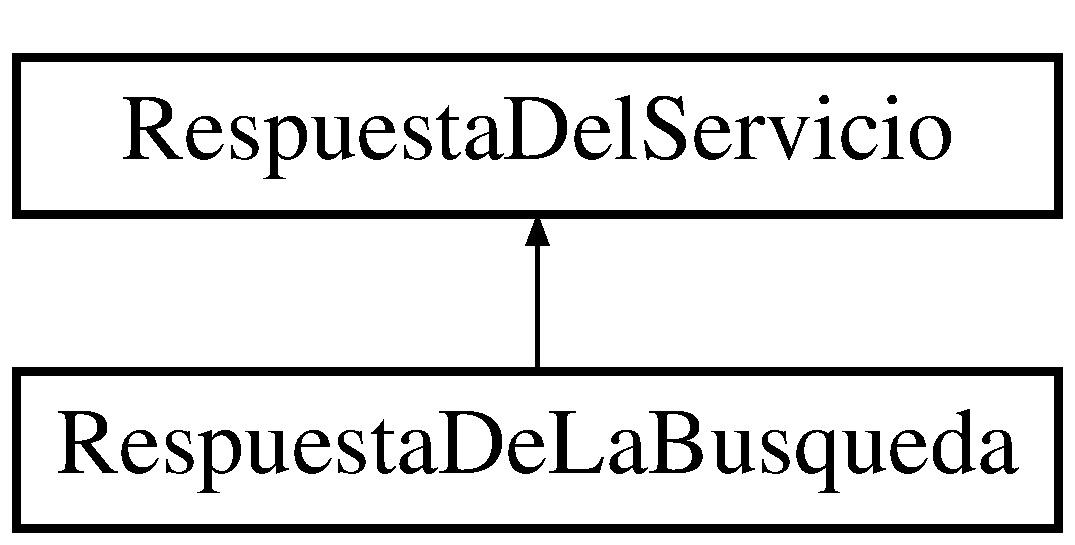
\includegraphics[height=2.000000cm]{classRespuestaDeLaBusqueda}
\end{center}
\end{figure}
\subsection*{Public Member Functions}
\begin{DoxyCompactItemize}
\item 
void {\bfseries set\+Respuesta\+Candidato\+Encontrado} (\hyperlink{classUsuario}{Usuario} $\ast$usuario)\hypertarget{classRespuestaDeLaBusqueda_a489698777a915943f7a92d1d4277e352}{}\label{classRespuestaDeLaBusqueda_a489698777a915943f7a92d1d4277e352}

\item 
void {\bfseries set\+Respuesta\+Candidato\+No\+Encontrado} ()\hypertarget{classRespuestaDeLaBusqueda_af8e37fb7da8b74e0ec8e29db493d19a9}{}\label{classRespuestaDeLaBusqueda_af8e37fb7da8b74e0ec8e29db493d19a9}

\end{DoxyCompactItemize}
\subsection*{Additional Inherited Members}


The documentation for this class was generated from the following files\+:\begin{DoxyCompactItemize}
\item 
Appserver/src/servicios/Respuesta\+De\+La\+Busqueda.\+h\item 
Appserver/src/servicios/Respuesta\+De\+La\+Busqueda.\+cpp\end{DoxyCompactItemize}

\hypertarget{classRespuestaDeLaVotacion}{}\section{Respuesta\+De\+La\+Votacion Class Reference}
\label{classRespuestaDeLaVotacion}\index{Respuesta\+De\+La\+Votacion@{Respuesta\+De\+La\+Votacion}}
Inheritance diagram for Respuesta\+De\+La\+Votacion\+:\begin{figure}[H]
\begin{center}
\leavevmode
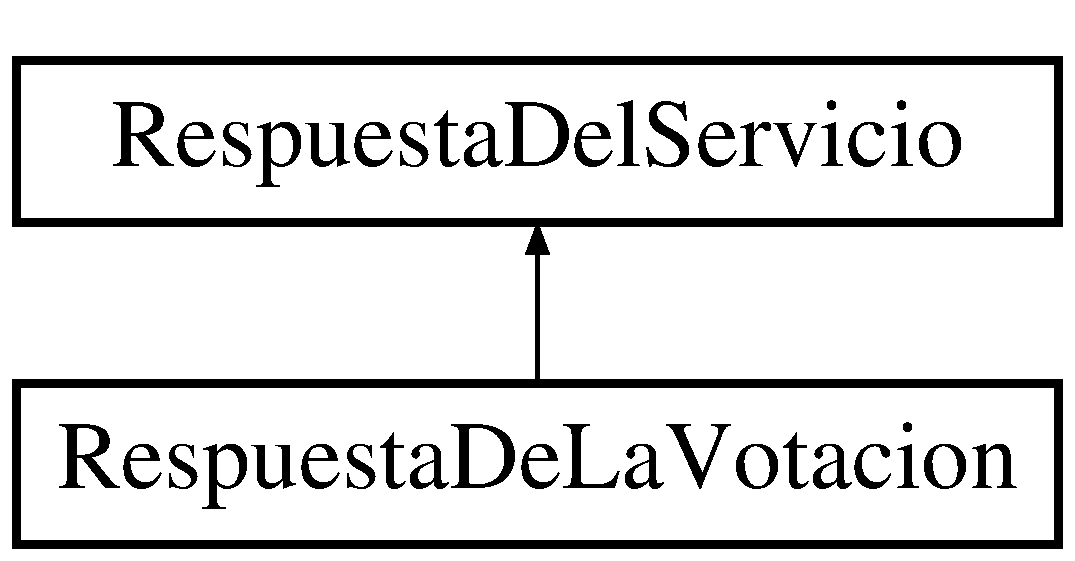
\includegraphics[height=2.000000cm]{classRespuestaDeLaVotacion}
\end{center}
\end{figure}
\subsection*{Public Member Functions}
\begin{DoxyCompactItemize}
\item 
void {\bfseries set\+Respuesta\+Se\+Registro\+Voto} ()\hypertarget{classRespuestaDeLaVotacion_aed9b86c5d70e506716961f6bc5f4cc80}{}\label{classRespuestaDeLaVotacion_aed9b86c5d70e506716961f6bc5f4cc80}

\end{DoxyCompactItemize}
\subsection*{Additional Inherited Members}


The documentation for this class was generated from the following files\+:\begin{DoxyCompactItemize}
\item 
Appserver/src/servicios/Respuesta\+De\+La\+Votacion.\+h\item 
Appserver/src/servicios/Respuesta\+De\+La\+Votacion.\+cpp\end{DoxyCompactItemize}

\hypertarget{classRespuestaDelChat}{}\section{Respuesta\+Del\+Chat Class Reference}
\label{classRespuestaDelChat}\index{Respuesta\+Del\+Chat@{Respuesta\+Del\+Chat}}
Inheritance diagram for Respuesta\+Del\+Chat\+:\begin{figure}[H]
\begin{center}
\leavevmode
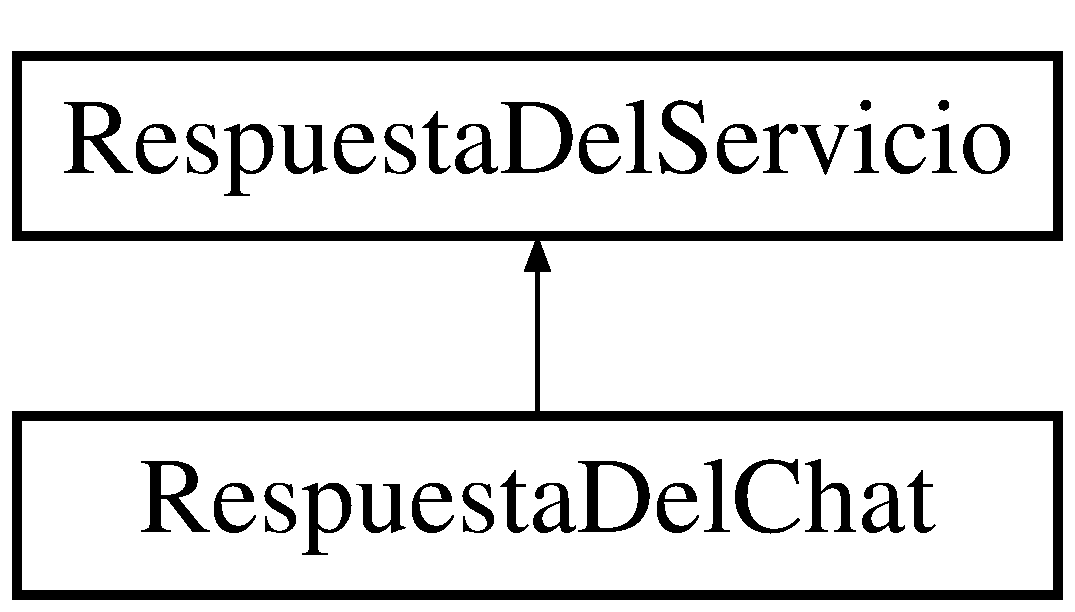
\includegraphics[height=2.000000cm]{classRespuestaDelChat}
\end{center}
\end{figure}
\subsection*{Public Member Functions}
\begin{DoxyCompactItemize}
\item 
void {\bfseries set\+Respuesta\+G\+CM} ()\hypertarget{classRespuestaDelChat_a53a20f3049b1a7fa51a9a19500184810}{}\label{classRespuestaDelChat_a53a20f3049b1a7fa51a9a19500184810}

\end{DoxyCompactItemize}
\subsection*{Additional Inherited Members}


The documentation for this class was generated from the following files\+:\begin{DoxyCompactItemize}
\item 
Appserver/src/servicios/Respuesta\+Del\+Chat.\+h\item 
Appserver/src/servicios/Respuesta\+Del\+Chat.\+cpp\end{DoxyCompactItemize}

\hypertarget{classRespuestaDelLogin}{}\section{Respuesta\+Del\+Login Class Reference}
\label{classRespuestaDelLogin}\index{Respuesta\+Del\+Login@{Respuesta\+Del\+Login}}
Inheritance diagram for Respuesta\+Del\+Login\+:\begin{figure}[H]
\begin{center}
\leavevmode
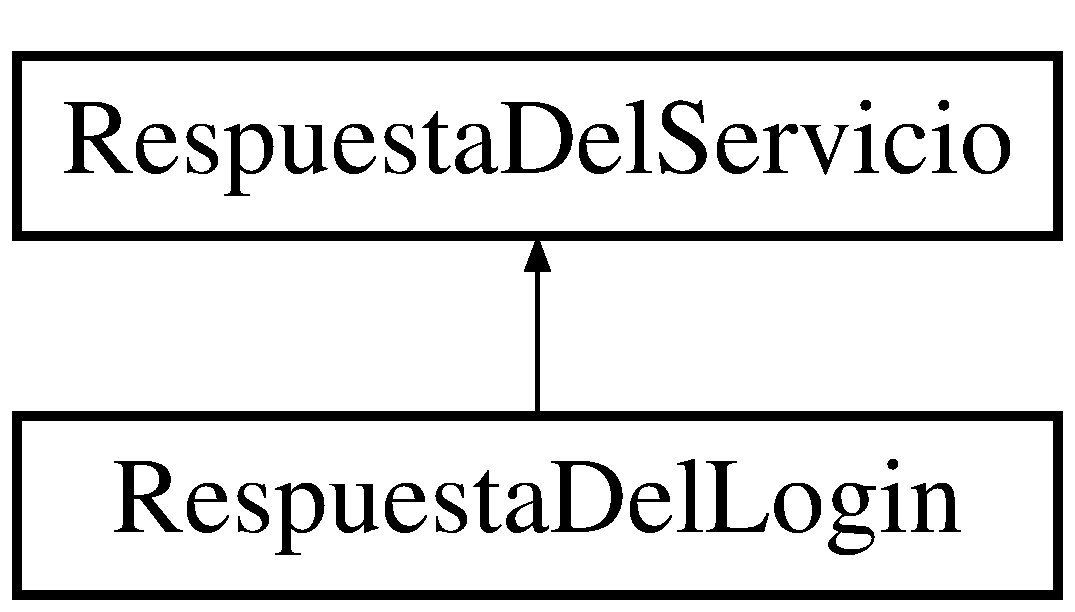
\includegraphics[height=2.000000cm]{classRespuestaDelLogin}
\end{center}
\end{figure}
\subsection*{Public Member Functions}
\begin{DoxyCompactItemize}
\item 
void {\bfseries set\+Respuesta\+Login\+Correcto} (string token)\hypertarget{classRespuestaDelLogin_a350ec1b94bfa7ab5510001b48f63f110}{}\label{classRespuestaDelLogin_a350ec1b94bfa7ab5510001b48f63f110}

\item 
void {\bfseries set\+Respuesta\+Login\+Incorrecto} ()\hypertarget{classRespuestaDelLogin_a890dd2d91994441c0e309c99fcc60147}{}\label{classRespuestaDelLogin_a890dd2d91994441c0e309c99fcc60147}

\end{DoxyCompactItemize}
\subsection*{Additional Inherited Members}


The documentation for this class was generated from the following files\+:\begin{DoxyCompactItemize}
\item 
Appserver/src/servicios/Respuesta\+Del\+Login.\+h\item 
Appserver/src/servicios/Respuesta\+Del\+Login.\+cpp\end{DoxyCompactItemize}

\hypertarget{classRespuestaDelRegistro}{}\section{Respuesta\+Del\+Registro Class Reference}
\label{classRespuestaDelRegistro}\index{Respuesta\+Del\+Registro@{Respuesta\+Del\+Registro}}
Inheritance diagram for Respuesta\+Del\+Registro\+:\begin{figure}[H]
\begin{center}
\leavevmode
\includegraphics[height=2.000000cm]{classRespuestaDelRegistro}
\end{center}
\end{figure}
\subsection*{Public Member Functions}
\begin{DoxyCompactItemize}
\item 
void {\bfseries set\+Respuesta\+Usuario\+Existente} ()\hypertarget{classRespuestaDelRegistro_ab76e3e0d237ce4435f841fe0986271dc}{}\label{classRespuestaDelRegistro_ab76e3e0d237ce4435f841fe0986271dc}

\item 
void {\bfseries set\+Respuesta\+Error\+Del\+Shared\+Server} ()\hypertarget{classRespuestaDelRegistro_a837a60bb365b0dcefdc2cd5973e07cb1}{}\label{classRespuestaDelRegistro_a837a60bb365b0dcefdc2cd5973e07cb1}

\item 
void {\bfseries set\+Respuesta\+Registro\+Correcto} ()\hypertarget{classRespuestaDelRegistro_a0af860cc761325577aebc936286868e8}{}\label{classRespuestaDelRegistro_a0af860cc761325577aebc936286868e8}

\end{DoxyCompactItemize}
\subsection*{Additional Inherited Members}


The documentation for this class was generated from the following files\+:\begin{DoxyCompactItemize}
\item 
Appserver/src/servicios/Respuesta\+Del\+Registro.\+h\item 
Appserver/src/servicios/Respuesta\+Del\+Registro.\+cpp\end{DoxyCompactItemize}

\hypertarget{classRespuestaDelServicio}{}\section{Respuesta\+Del\+Servicio Class Reference}
\label{classRespuestaDelServicio}\index{Respuesta\+Del\+Servicio@{Respuesta\+Del\+Servicio}}
Inheritance diagram for Respuesta\+Del\+Servicio\+:\begin{figure}[H]
\begin{center}
\leavevmode
\includegraphics[height=10.000000cm]{classRespuestaDelServicio}
\end{center}
\end{figure}
\subsection*{Public Member Functions}
\begin{DoxyCompactItemize}
\item 
string {\bfseries to\+String} ()\hypertarget{classRespuestaDelServicio_ab78ab6696438b9c62350750a5c4ca417}{}\label{classRespuestaDelServicio_ab78ab6696438b9c62350750a5c4ca417}

\end{DoxyCompactItemize}
\subsection*{Protected Attributes}
\begin{DoxyCompactItemize}
\item 
\hyperlink{classMensajeHTTPReply}{Mensaje\+H\+T\+T\+P\+Reply} {\bfseries respuesta}\hypertarget{classRespuestaDelServicio_af0086a8d7b4cbf4bc6a62d2548a7db52}{}\label{classRespuestaDelServicio_af0086a8d7b4cbf4bc6a62d2548a7db52}

\end{DoxyCompactItemize}


The documentation for this class was generated from the following files\+:\begin{DoxyCompactItemize}
\item 
Appserver/src/servicios/Respuesta\+Del\+Servicio.\+h\item 
Appserver/src/servicios/Respuesta\+Del\+Servicio.\+cpp\end{DoxyCompactItemize}

\hypertarget{classRespuestaEliminacion}{}\section{Respuesta\+Eliminacion Class Reference}
\label{classRespuestaEliminacion}\index{Respuesta\+Eliminacion@{Respuesta\+Eliminacion}}
Inheritance diagram for Respuesta\+Eliminacion\+:\begin{figure}[H]
\begin{center}
\leavevmode
\includegraphics[height=2.000000cm]{classRespuestaEliminacion}
\end{center}
\end{figure}
\subsection*{Public Member Functions}
\begin{DoxyCompactItemize}
\item 
void {\bfseries set\+Respuesta\+Eliminacion\+Correcta} ()\hypertarget{classRespuestaEliminacion_a325283366c4fa4aeb1cf754a69c13276}{}\label{classRespuestaEliminacion_a325283366c4fa4aeb1cf754a69c13276}

\item 
void {\bfseries set\+Respuesta\+Eliminacion\+Incorrecta} ()\hypertarget{classRespuestaEliminacion_a50e939dbaf3e9be150319fc9a0581aa3}{}\label{classRespuestaEliminacion_a50e939dbaf3e9be150319fc9a0581aa3}

\end{DoxyCompactItemize}
\subsection*{Additional Inherited Members}


The documentation for this class was generated from the following files\+:\begin{DoxyCompactItemize}
\item 
Appserver/src/servicios/Respuesta\+Eliminacion.\+h\item 
Appserver/src/servicios/Respuesta\+Eliminacion.\+cpp\end{DoxyCompactItemize}

\hypertarget{classRespuestaMensajes}{}\section{Respuesta\+Mensajes Class Reference}
\label{classRespuestaMensajes}\index{Respuesta\+Mensajes@{Respuesta\+Mensajes}}
Inheritance diagram for Respuesta\+Mensajes\+:\begin{figure}[H]
\begin{center}
\leavevmode
\includegraphics[height=2.000000cm]{classRespuestaMensajes}
\end{center}
\end{figure}
\subsection*{Public Member Functions}
\begin{DoxyCompactItemize}
\item 
void {\bfseries set\+Mensajes\+Como\+Respuesta} (\hyperlink{classMensajes}{Mensajes} \&mensajes)\hypertarget{classRespuestaMensajes_a5ee62af5035eba3b4ccb9f27d64bc72f}{}\label{classRespuestaMensajes_a5ee62af5035eba3b4ccb9f27d64bc72f}

\end{DoxyCompactItemize}
\subsection*{Additional Inherited Members}


The documentation for this class was generated from the following files\+:\begin{DoxyCompactItemize}
\item 
Appserver/src/servicios/Respuesta\+Mensajes.\+h\item 
Appserver/src/servicios/Respuesta\+Mensajes.\+cpp\end{DoxyCompactItemize}

\hypertarget{classRespuestaModificarFoto}{}\section{Respuesta\+Modificar\+Foto Class Reference}
\label{classRespuestaModificarFoto}\index{Respuesta\+Modificar\+Foto@{Respuesta\+Modificar\+Foto}}
Inheritance diagram for Respuesta\+Modificar\+Foto\+:\begin{figure}[H]
\begin{center}
\leavevmode
\includegraphics[height=2.000000cm]{classRespuestaModificarFoto}
\end{center}
\end{figure}
\subsection*{Public Member Functions}
\begin{DoxyCompactItemize}
\item 
void {\bfseries set\+Respuesta\+Modificacion\+Correcta} ()\hypertarget{classRespuestaModificarFoto_a59021878e7bc6c7856fe33ab91941b6b}{}\label{classRespuestaModificarFoto_a59021878e7bc6c7856fe33ab91941b6b}

\item 
void {\bfseries set\+Respuesta\+Modificacion\+Incorrecta} ()\hypertarget{classRespuestaModificarFoto_a3b3c562f9eedd98b8980e107bbf5488b}{}\label{classRespuestaModificarFoto_a3b3c562f9eedd98b8980e107bbf5488b}

\end{DoxyCompactItemize}
\subsection*{Additional Inherited Members}


The documentation for this class was generated from the following files\+:\begin{DoxyCompactItemize}
\item 
Appserver/src/servicios/Respuesta\+Modificar\+Foto.\+h\item 
Appserver/src/servicios/Respuesta\+Modificar\+Foto.\+cpp\end{DoxyCompactItemize}

\hypertarget{classRespuestaServicioInexistente}{}\section{Respuesta\+Servicio\+Inexistente Class Reference}
\label{classRespuestaServicioInexistente}\index{Respuesta\+Servicio\+Inexistente@{Respuesta\+Servicio\+Inexistente}}
Inheritance diagram for Respuesta\+Servicio\+Inexistente\+:\begin{figure}[H]
\begin{center}
\leavevmode
\includegraphics[height=2.000000cm]{classRespuestaServicioInexistente}
\end{center}
\end{figure}
\subsection*{Additional Inherited Members}


The documentation for this class was generated from the following files\+:\begin{DoxyCompactItemize}
\item 
Appserver/src/servicios/Respuesta\+Servicio\+Inexistente.\+h\item 
Appserver/src/servicios/Respuesta\+Servicio\+Inexistente.\+cpp\end{DoxyCompactItemize}

\hypertarget{classrocksdb_1_1RestoreBackupableDB}{}\section{rocksdb\+:\+:Restore\+Backupable\+DB Class Reference}
\label{classrocksdb_1_1RestoreBackupableDB}\index{rocksdb\+::\+Restore\+Backupable\+DB@{rocksdb\+::\+Restore\+Backupable\+DB}}
\subsection*{Public Member Functions}
\begin{DoxyCompactItemize}
\item 
{\bfseries Restore\+Backupable\+DB} (\hyperlink{classrocksdb_1_1Env}{Env} $\ast$db\+\_\+env, const \hyperlink{structrocksdb_1_1BackupableDBOptions}{Backupable\+D\+B\+Options} \&options)\hypertarget{classrocksdb_1_1RestoreBackupableDB_a99288ae06ea295685e8adf70d3d2cdb6}{}\label{classrocksdb_1_1RestoreBackupableDB_a99288ae06ea295685e8adf70d3d2cdb6}

\item 
void {\bfseries Get\+Backup\+Info} (std\+::vector$<$ \hyperlink{structrocksdb_1_1BackupInfo}{Backup\+Info} $>$ $\ast$backup\+\_\+info)\hypertarget{classrocksdb_1_1RestoreBackupableDB_a17d272e67c518523c5d61301b78daa99}{}\label{classrocksdb_1_1RestoreBackupableDB_a17d272e67c518523c5d61301b78daa99}

\item 
void {\bfseries Get\+Corrupted\+Backups} (std\+::vector$<$ Backup\+ID $>$ $\ast$corrupt\+\_\+backup\+\_\+ids)\hypertarget{classrocksdb_1_1RestoreBackupableDB_acbc4fd7ca4193eb8b9ef2637d484805c}{}\label{classrocksdb_1_1RestoreBackupableDB_acbc4fd7ca4193eb8b9ef2637d484805c}

\item 
\hyperlink{classrocksdb_1_1Status}{Status} {\bfseries Restore\+D\+B\+From\+Backup} (Backup\+ID backup\+\_\+id, const std\+::string \&db\+\_\+dir, const std\+::string \&wal\+\_\+dir, const \hyperlink{structrocksdb_1_1RestoreOptions}{Restore\+Options} \&restore\+\_\+options=\hyperlink{structrocksdb_1_1RestoreOptions}{Restore\+Options}())\hypertarget{classrocksdb_1_1RestoreBackupableDB_aac7e79522516f2685877eb0b2a034490}{}\label{classrocksdb_1_1RestoreBackupableDB_aac7e79522516f2685877eb0b2a034490}

\item 
\hyperlink{classrocksdb_1_1Status}{Status} {\bfseries Restore\+D\+B\+From\+Latest\+Backup} (const std\+::string \&db\+\_\+dir, const std\+::string \&wal\+\_\+dir, const \hyperlink{structrocksdb_1_1RestoreOptions}{Restore\+Options} \&restore\+\_\+options=\hyperlink{structrocksdb_1_1RestoreOptions}{Restore\+Options}())\hypertarget{classrocksdb_1_1RestoreBackupableDB_abe5e355e3185131a77cc358d99fe4558}{}\label{classrocksdb_1_1RestoreBackupableDB_abe5e355e3185131a77cc358d99fe4558}

\item 
\hyperlink{classrocksdb_1_1Status}{Status} {\bfseries Purge\+Old\+Backups} (uint32\+\_\+t num\+\_\+backups\+\_\+to\+\_\+keep)\hypertarget{classrocksdb_1_1RestoreBackupableDB_a8568545789fdcb4f707c61b711993d92}{}\label{classrocksdb_1_1RestoreBackupableDB_a8568545789fdcb4f707c61b711993d92}

\item 
\hyperlink{classrocksdb_1_1Status}{Status} {\bfseries Delete\+Backup} (Backup\+ID backup\+\_\+id)\hypertarget{classrocksdb_1_1RestoreBackupableDB_aeb3b0a390232dfbfb2676652b40ce7e5}{}\label{classrocksdb_1_1RestoreBackupableDB_aeb3b0a390232dfbfb2676652b40ce7e5}

\item 
\hyperlink{classrocksdb_1_1Status}{Status} {\bfseries Garbage\+Collect} ()\hypertarget{classrocksdb_1_1RestoreBackupableDB_a5a27018727fd65724bbf0d2c083ffea8}{}\label{classrocksdb_1_1RestoreBackupableDB_a5a27018727fd65724bbf0d2c083ffea8}

\end{DoxyCompactItemize}


The documentation for this class was generated from the following file\+:\begin{DoxyCompactItemize}
\item 
Appserver/src/external/rocksdb/utilities/backupable\+\_\+db.\+h\end{DoxyCompactItemize}

\hypertarget{structrocksdb_1_1RestoreOptions}{}\section{rocksdb\+:\+:Restore\+Options Struct Reference}
\label{structrocksdb_1_1RestoreOptions}\index{rocksdb\+::\+Restore\+Options@{rocksdb\+::\+Restore\+Options}}
\subsection*{Public Member Functions}
\begin{DoxyCompactItemize}
\item 
{\bfseries Restore\+Options} (bool \+\_\+keep\+\_\+log\+\_\+files=false)\hypertarget{structrocksdb_1_1RestoreOptions_abaf8129611f7174ab666932162674343}{}\label{structrocksdb_1_1RestoreOptions_abaf8129611f7174ab666932162674343}

\end{DoxyCompactItemize}
\subsection*{Public Attributes}
\begin{DoxyCompactItemize}
\item 
bool {\bfseries keep\+\_\+log\+\_\+files}\hypertarget{structrocksdb_1_1RestoreOptions_a1afaba5beaee9776bea92d5c48e55020}{}\label{structrocksdb_1_1RestoreOptions_a1afaba5beaee9776bea92d5c48e55020}

\end{DoxyCompactItemize}


The documentation for this struct was generated from the following file\+:\begin{DoxyCompactItemize}
\item 
Appserver/src/external/rocksdb/utilities/backupable\+\_\+db.\+h\end{DoxyCompactItemize}

\hypertarget{classJson_1_1RuntimeError}{}\section{Json\+:\+:Runtime\+Error Class Reference}
\label{classJson_1_1RuntimeError}\index{Json\+::\+Runtime\+Error@{Json\+::\+Runtime\+Error}}


{\ttfamily \#include $<$json.\+h$>$}

Inheritance diagram for Json\+:\+:Runtime\+Error\+:\begin{figure}[H]
\begin{center}
\leavevmode
\includegraphics[height=3.000000cm]{classJson_1_1RuntimeError}
\end{center}
\end{figure}
\subsection*{Public Member Functions}
\begin{DoxyCompactItemize}
\item 
{\bfseries Runtime\+Error} (J\+S\+O\+N\+C\+P\+P\+\_\+\+S\+T\+R\+I\+NG const \&msg)\hypertarget{classJson_1_1RuntimeError_a0f6445dc345ce0a703610b6e893fee40}{}\label{classJson_1_1RuntimeError_a0f6445dc345ce0a703610b6e893fee40}

\end{DoxyCompactItemize}
\subsection*{Additional Inherited Members}


\subsection{Detailed Description}
Exceptions which the user cannot easily avoid.

E.\+g. out-\/of-\/memory (when we use malloc), stack-\/overflow, malicious input

\begin{DoxyRemark}{Remarks}
derived from \hyperlink{classJson_1_1Exception}{Json\+::\+Exception} 
\end{DoxyRemark}


The documentation for this class was generated from the following files\+:\begin{DoxyCompactItemize}
\item 
Appserver/src/external/json/json.\+h\item 
Appserver/src/external/json/jsoncpp.\+cpp\end{DoxyCompactItemize}

\hypertarget{classJson_1_1SecureAllocator}{}\section{Json\+:\+:Secure\+Allocator$<$ T $>$ Class Template Reference}
\label{classJson_1_1SecureAllocator}\index{Json\+::\+Secure\+Allocator$<$ T $>$@{Json\+::\+Secure\+Allocator$<$ T $>$}}
\subsection*{Classes}
\begin{DoxyCompactItemize}
\item 
struct \hyperlink{structJson_1_1SecureAllocator_1_1rebind}{rebind}
\end{DoxyCompactItemize}
\subsection*{Public Types}
\begin{DoxyCompactItemize}
\item 
using {\bfseries value\+\_\+type} = T\hypertarget{classJson_1_1SecureAllocator_ae45a020fc6d6f3ae66394c81c4281ad8}{}\label{classJson_1_1SecureAllocator_ae45a020fc6d6f3ae66394c81c4281ad8}

\item 
using {\bfseries pointer} = T $\ast$\hypertarget{classJson_1_1SecureAllocator_a442c09b3267622d23416d9072ea1afe9}{}\label{classJson_1_1SecureAllocator_a442c09b3267622d23416d9072ea1afe9}

\item 
using {\bfseries const\+\_\+pointer} = const T $\ast$\hypertarget{classJson_1_1SecureAllocator_a464b356817c78ea996cd3a7403f7e735}{}\label{classJson_1_1SecureAllocator_a464b356817c78ea996cd3a7403f7e735}

\item 
using {\bfseries reference} = T \&\hypertarget{classJson_1_1SecureAllocator_a55b243c56812b3852b59c1a9b0a21c65}{}\label{classJson_1_1SecureAllocator_a55b243c56812b3852b59c1a9b0a21c65}

\item 
using {\bfseries const\+\_\+reference} = const T \&\hypertarget{classJson_1_1SecureAllocator_a3f0327d609dcd1942c8c7fa4d4f227e5}{}\label{classJson_1_1SecureAllocator_a3f0327d609dcd1942c8c7fa4d4f227e5}

\item 
using {\bfseries size\+\_\+type} = std\+::size\+\_\+t\hypertarget{classJson_1_1SecureAllocator_a61c258f0ae80af6982fae200b55a4dc9}{}\label{classJson_1_1SecureAllocator_a61c258f0ae80af6982fae200b55a4dc9}

\item 
using {\bfseries difference\+\_\+type} = std\+::ptrdiff\+\_\+t\hypertarget{classJson_1_1SecureAllocator_a404f41a8e340a8af1b54138920a6ef33}{}\label{classJson_1_1SecureAllocator_a404f41a8e340a8af1b54138920a6ef33}

\end{DoxyCompactItemize}
\subsection*{Public Member Functions}
\begin{DoxyCompactItemize}
\item 
pointer \hyperlink{classJson_1_1SecureAllocator_a9b7d7180b360ebd673bdcfab25c1d5a4}{allocate} (size\+\_\+type n)
\item 
void \hyperlink{classJson_1_1SecureAllocator_a93c86d9e9031b81a046b3db8897811f2}{deallocate} (volatile pointer p, size\+\_\+type n)
\item 
{\footnotesize template$<$typename... Args$>$ }\\void \hyperlink{classJson_1_1SecureAllocator_acd466192ba41ea5468bd2f45ae9de9fb}{construct} (pointer p, Args \&\&... args)
\item 
size\+\_\+type {\bfseries max\+\_\+size} () const\hypertarget{classJson_1_1SecureAllocator_a1ca352414d0ce358c0dca70fb26c674c}{}\label{classJson_1_1SecureAllocator_a1ca352414d0ce358c0dca70fb26c674c}

\item 
pointer {\bfseries address} (reference x) const\hypertarget{classJson_1_1SecureAllocator_a2f26b3dbf3cfffcc376844fb19733422}{}\label{classJson_1_1SecureAllocator_a2f26b3dbf3cfffcc376844fb19733422}

\item 
const\+\_\+pointer {\bfseries address} (const\+\_\+reference x) const\hypertarget{classJson_1_1SecureAllocator_a228944048dd7266f219b52fd1958b4d5}{}\label{classJson_1_1SecureAllocator_a228944048dd7266f219b52fd1958b4d5}

\item 
void \hyperlink{classJson_1_1SecureAllocator_a7316f4efeb3b992c69c94e345ac9f5cd}{destroy} (pointer p)
\item 
{\footnotesize template$<$typename U $>$ }\\{\bfseries Secure\+Allocator} (const \hyperlink{classJson_1_1SecureAllocator}{Secure\+Allocator}$<$ U $>$ \&)\hypertarget{classJson_1_1SecureAllocator_afefbe83997eb1da2089229771957e6bd}{}\label{classJson_1_1SecureAllocator_afefbe83997eb1da2089229771957e6bd}

\end{DoxyCompactItemize}


\subsection{Member Function Documentation}
\index{Json\+::\+Secure\+Allocator@{Json\+::\+Secure\+Allocator}!allocate@{allocate}}
\index{allocate@{allocate}!Json\+::\+Secure\+Allocator@{Json\+::\+Secure\+Allocator}}
\subsubsection[{\texorpdfstring{allocate(size\+\_\+type n)}{allocate(size\_type n)}}]{\setlength{\rightskip}{0pt plus 5cm}template$<$typename T $>$ pointer {\bf Json\+::\+Secure\+Allocator}$<$ T $>$\+::allocate (
\begin{DoxyParamCaption}
\item[{size\+\_\+type}]{n}
\end{DoxyParamCaption}
)\hspace{0.3cm}{\ttfamily [inline]}}\hypertarget{classJson_1_1SecureAllocator_a9b7d7180b360ebd673bdcfab25c1d5a4}{}\label{classJson_1_1SecureAllocator_a9b7d7180b360ebd673bdcfab25c1d5a4}
Allocate memory for N items using the standard allocator. \index{Json\+::\+Secure\+Allocator@{Json\+::\+Secure\+Allocator}!construct@{construct}}
\index{construct@{construct}!Json\+::\+Secure\+Allocator@{Json\+::\+Secure\+Allocator}}
\subsubsection[{\texorpdfstring{construct(pointer p, Args \&\&... args)}{construct(pointer p, Args \&\&... args)}}]{\setlength{\rightskip}{0pt plus 5cm}template$<$typename T $>$ template$<$typename... Args$>$ void {\bf Json\+::\+Secure\+Allocator}$<$ T $>$\+::construct (
\begin{DoxyParamCaption}
\item[{pointer}]{p, }
\item[{Args \&\&...}]{args}
\end{DoxyParamCaption}
)\hspace{0.3cm}{\ttfamily [inline]}}\hypertarget{classJson_1_1SecureAllocator_acd466192ba41ea5468bd2f45ae9de9fb}{}\label{classJson_1_1SecureAllocator_acd466192ba41ea5468bd2f45ae9de9fb}
Construct an item in-\/place at pointer P. \index{Json\+::\+Secure\+Allocator@{Json\+::\+Secure\+Allocator}!deallocate@{deallocate}}
\index{deallocate@{deallocate}!Json\+::\+Secure\+Allocator@{Json\+::\+Secure\+Allocator}}
\subsubsection[{\texorpdfstring{deallocate(volatile pointer p, size\+\_\+type n)}{deallocate(volatile pointer p, size\_type n)}}]{\setlength{\rightskip}{0pt plus 5cm}template$<$typename T $>$ void {\bf Json\+::\+Secure\+Allocator}$<$ T $>$\+::deallocate (
\begin{DoxyParamCaption}
\item[{volatile pointer}]{p, }
\item[{size\+\_\+type}]{n}
\end{DoxyParamCaption}
)\hspace{0.3cm}{\ttfamily [inline]}}\hypertarget{classJson_1_1SecureAllocator_a93c86d9e9031b81a046b3db8897811f2}{}\label{classJson_1_1SecureAllocator_a93c86d9e9031b81a046b3db8897811f2}
Release memory which was allocated for N items at pointer P.

The memory block is filled with zeroes before being released. The pointer argument is tagged as \char`\"{}volatile\char`\"{} to prevent the compiler optimizing out this critical step. \index{Json\+::\+Secure\+Allocator@{Json\+::\+Secure\+Allocator}!destroy@{destroy}}
\index{destroy@{destroy}!Json\+::\+Secure\+Allocator@{Json\+::\+Secure\+Allocator}}
\subsubsection[{\texorpdfstring{destroy(pointer p)}{destroy(pointer p)}}]{\setlength{\rightskip}{0pt plus 5cm}template$<$typename T $>$ void {\bf Json\+::\+Secure\+Allocator}$<$ T $>$\+::destroy (
\begin{DoxyParamCaption}
\item[{pointer}]{p}
\end{DoxyParamCaption}
)\hspace{0.3cm}{\ttfamily [inline]}}\hypertarget{classJson_1_1SecureAllocator_a7316f4efeb3b992c69c94e345ac9f5cd}{}\label{classJson_1_1SecureAllocator_a7316f4efeb3b992c69c94e345ac9f5cd}
Destroy an item in-\/place at pointer P. 

The documentation for this class was generated from the following file\+:\begin{DoxyCompactItemize}
\item 
Appserver/src/external/json/json.\+h\end{DoxyCompactItemize}

\hypertarget{classrocksdb_1_1SequentialFile}{}\section{rocksdb\+:\+:Sequential\+File Class Reference}
\label{classrocksdb_1_1SequentialFile}\index{rocksdb\+::\+Sequential\+File@{rocksdb\+::\+Sequential\+File}}
\subsection*{Public Member Functions}
\begin{DoxyCompactItemize}
\item 
virtual \hyperlink{classrocksdb_1_1Status}{Status} {\bfseries Read} (size\+\_\+t n, \hyperlink{classrocksdb_1_1Slice}{Slice} $\ast$result, char $\ast$scratch)=0\hypertarget{classrocksdb_1_1SequentialFile_a73ad8155e9996d5430081aaac7eb0d00}{}\label{classrocksdb_1_1SequentialFile_a73ad8155e9996d5430081aaac7eb0d00}

\item 
virtual \hyperlink{classrocksdb_1_1Status}{Status} {\bfseries Skip} (uint64\+\_\+t n)=0\hypertarget{classrocksdb_1_1SequentialFile_a7631793bdbfe43ddbd7a5326939c056a}{}\label{classrocksdb_1_1SequentialFile_a7631793bdbfe43ddbd7a5326939c056a}

\item 
virtual \hyperlink{classrocksdb_1_1Status}{Status} {\bfseries Invalidate\+Cache} (size\+\_\+t offset, size\+\_\+t length)\hypertarget{classrocksdb_1_1SequentialFile_aed3847c9352221eba27eb9c58fe2d287}{}\label{classrocksdb_1_1SequentialFile_aed3847c9352221eba27eb9c58fe2d287}

\end{DoxyCompactItemize}


The documentation for this class was generated from the following file\+:\begin{DoxyCompactItemize}
\item 
Appserver/src/external/rocksdb/env.\+h\end{DoxyCompactItemize}

\hypertarget{classServicio}{}\section{Servicio Class Reference}
\label{classServicio}\index{Servicio@{Servicio}}
Inheritance diagram for Servicio\+:\begin{figure}[H]
\begin{center}
\leavevmode
\includegraphics[height=10.000000cm]{classServicio}
\end{center}
\end{figure}
\subsection*{Public Member Functions}
\begin{DoxyCompactItemize}
\item 
\hyperlink{classRespuestaDelServicio}{Respuesta\+Del\+Servicio} $\ast$ {\bfseries get\+Respuesta} ()\hypertarget{classServicio_a31441550855a7ba54b1a24f7187103d1}{}\label{classServicio_a31441550855a7ba54b1a24f7187103d1}

\end{DoxyCompactItemize}
\subsection*{Protected Attributes}
\begin{DoxyCompactItemize}
\item 
\hyperlink{classRespuestaDelServicio}{Respuesta\+Del\+Servicio} $\ast$ {\bfseries respuesta}\hypertarget{classServicio_a0bdb37ede65289e8508939786de91277}{}\label{classServicio_a0bdb37ede65289e8508939786de91277}

\end{DoxyCompactItemize}


The documentation for this class was generated from the following files\+:\begin{DoxyCompactItemize}
\item 
Appserver/src/servicios/Servicio.\+h\item 
Appserver/src/servicios/Servicio.\+cpp\end{DoxyCompactItemize}

\hypertarget{classServicioBusquedaCandidatos}{}\section{Servicio\+Busqueda\+Candidatos Class Reference}
\label{classServicioBusquedaCandidatos}\index{Servicio\+Busqueda\+Candidatos@{Servicio\+Busqueda\+Candidatos}}
Inheritance diagram for Servicio\+Busqueda\+Candidatos\+:\begin{figure}[H]
\begin{center}
\leavevmode
\includegraphics[height=2.000000cm]{classServicioBusquedaCandidatos}
\end{center}
\end{figure}
\subsection*{Public Member Functions}
\begin{DoxyCompactItemize}
\item 
{\bfseries Servicio\+Busqueda\+Candidatos} (\hyperlink{classAdministradorCandidatos}{Administrador\+Candidatos} $\ast$administrador\+Candidatos, \hyperlink{classMensajeHTTPRequest}{Mensaje\+H\+T\+T\+P\+Request} $\ast$mensaje\+H\+T\+TP)\hypertarget{classServicioBusquedaCandidatos_a84dfbfc8f67a9969f34bd046ddfc5088}{}\label{classServicioBusquedaCandidatos_a84dfbfc8f67a9969f34bd046ddfc5088}

\end{DoxyCompactItemize}
\subsection*{Additional Inherited Members}


The documentation for this class was generated from the following files\+:\begin{DoxyCompactItemize}
\item 
Appserver/src/servicios/Servicio\+Busqueda\+Candidatos.\+h\item 
Appserver/src/servicios/Servicio\+Busqueda\+Candidatos.\+cpp\end{DoxyCompactItemize}

\hypertarget{classServicioChat}{}\section{Servicio\+Chat Class Reference}
\label{classServicioChat}\index{Servicio\+Chat@{Servicio\+Chat}}
Inheritance diagram for Servicio\+Chat\+:\begin{figure}[H]
\begin{center}
\leavevmode
\includegraphics[height=2.000000cm]{classServicioChat}
\end{center}
\end{figure}
\subsection*{Public Member Functions}
\begin{DoxyCompactItemize}
\item 
{\bfseries Servicio\+Chat} (\hyperlink{classMensajero}{Mensajero} $\ast$mensajero, \hyperlink{classMensajeHTTPRequest}{Mensaje\+H\+T\+T\+P\+Request} $\ast$mensaje\+H\+T\+TP, \hyperlink{classSesionesDeUsuarios}{Sesiones\+De\+Usuarios} $\ast$sesiones, \hyperlink{classConversaciones}{Conversaciones} $\ast$conversaciones)\hypertarget{classServicioChat_a13e56b41c86b87501d4f242581a710cb}{}\label{classServicioChat_a13e56b41c86b87501d4f242581a710cb}

\end{DoxyCompactItemize}
\subsection*{Additional Inherited Members}


The documentation for this class was generated from the following files\+:\begin{DoxyCompactItemize}
\item 
Appserver/src/servicios/Servicio\+Chat.\+h\item 
Appserver/src/servicios/Servicio\+Chat.\+cpp\end{DoxyCompactItemize}

\hypertarget{classServicioEliminarUsuario}{}\section{Servicio\+Eliminar\+Usuario Class Reference}
\label{classServicioEliminarUsuario}\index{Servicio\+Eliminar\+Usuario@{Servicio\+Eliminar\+Usuario}}
Inheritance diagram for Servicio\+Eliminar\+Usuario\+:\begin{figure}[H]
\begin{center}
\leavevmode
\includegraphics[height=2.000000cm]{classServicioEliminarUsuario}
\end{center}
\end{figure}
\subsection*{Public Member Functions}
\begin{DoxyCompactItemize}
\item 
{\bfseries Servicio\+Eliminar\+Usuario} (\hyperlink{classSharedDataBase}{Shared\+Data\+Base} $\ast$shared, \hyperlink{classMensajeHTTPRequest}{Mensaje\+H\+T\+T\+P\+Request} $\ast$mensaje\+H\+T\+TP, \hyperlink{classCredencialesDeUsuarios}{Credenciales\+De\+Usuarios} $\ast$credenciales, \hyperlink{classSesionesDeUsuarios}{Sesiones\+De\+Usuarios} $\ast$sesiones)\hypertarget{classServicioEliminarUsuario_a3d9e074088d101735c9a024aac33a07e}{}\label{classServicioEliminarUsuario_a3d9e074088d101735c9a024aac33a07e}

\end{DoxyCompactItemize}
\subsection*{Additional Inherited Members}


The documentation for this class was generated from the following files\+:\begin{DoxyCompactItemize}
\item 
Appserver/src/servicios/Servicio\+Eliminar\+Usuario.\+h\item 
Appserver/src/servicios/Servicio\+Eliminar\+Usuario.\+cpp\end{DoxyCompactItemize}

\hypertarget{classServicioInexistente}{}\section{Servicio\+Inexistente Class Reference}
\label{classServicioInexistente}\index{Servicio\+Inexistente@{Servicio\+Inexistente}}
Inheritance diagram for Servicio\+Inexistente\+:\begin{figure}[H]
\begin{center}
\leavevmode
\includegraphics[height=2.000000cm]{classServicioInexistente}
\end{center}
\end{figure}
\subsection*{Additional Inherited Members}


The documentation for this class was generated from the following files\+:\begin{DoxyCompactItemize}
\item 
Appserver/src/servicios/Servicio\+Inexistente.\+h\item 
Appserver/src/servicios/Servicio\+Inexistente.\+cpp\end{DoxyCompactItemize}

\hypertarget{classservicioLogin}{}\section{servicio\+Login Class Reference}
\label{classservicioLogin}\index{servicio\+Login@{servicio\+Login}}
Inheritance diagram for servicio\+Login\+:\begin{figure}[H]
\begin{center}
\leavevmode
\includegraphics[height=2.000000cm]{classservicioLogin}
\end{center}
\end{figure}
\subsection*{Public Member Functions}
\begin{DoxyCompactItemize}
\item 
{\bfseries servicio\+Login} (\hyperlink{classSesionesDeUsuarios}{Sesiones\+De\+Usuarios} $\ast$sesiones\+De\+Usuarios, \hyperlink{classMensajeHTTPRequest}{Mensaje\+H\+T\+T\+P\+Request} mensaje\+H\+T\+TP, \hyperlink{classCredencialesDeUsuarios}{Credenciales\+De\+Usuarios} $\ast$credenciales)\hypertarget{classservicioLogin_a8987991d7cdd8b2ffa6aa9b802041c9f}{}\label{classservicioLogin_a8987991d7cdd8b2ffa6aa9b802041c9f}

\end{DoxyCompactItemize}
\subsection*{Additional Inherited Members}


The documentation for this class was generated from the following files\+:\begin{DoxyCompactItemize}
\item 
Appserver/src/servicios/servicio\+Login.\+h\item 
Appserver/src/servicios/servicio\+Login.\+cpp\end{DoxyCompactItemize}

\hypertarget{classServicioMensajes}{}\section{Servicio\+Mensajes Class Reference}
\label{classServicioMensajes}\index{Servicio\+Mensajes@{Servicio\+Mensajes}}
Inheritance diagram for Servicio\+Mensajes\+:\begin{figure}[H]
\begin{center}
\leavevmode
\includegraphics[height=2.000000cm]{classServicioMensajes}
\end{center}
\end{figure}
\subsection*{Public Member Functions}
\begin{DoxyCompactItemize}
\item 
{\bfseries Servicio\+Mensajes} (\hyperlink{classMensajeHTTPRequest}{Mensaje\+H\+T\+T\+P\+Request} $\ast$mensaje\+H\+T\+TP, \hyperlink{classSesionesDeUsuarios}{Sesiones\+De\+Usuarios} $\ast$sesiones, \hyperlink{classConversaciones}{Conversaciones} $\ast$conversaciones)\hypertarget{classServicioMensajes_acd9d4f5a54048bc0a95ca84e93ff1c28}{}\label{classServicioMensajes_acd9d4f5a54048bc0a95ca84e93ff1c28}

\end{DoxyCompactItemize}
\subsection*{Additional Inherited Members}


The documentation for this class was generated from the following files\+:\begin{DoxyCompactItemize}
\item 
Appserver/src/servicios/Servicio\+Mensajes.\+h\item 
Appserver/src/servicios/Servicio\+Mensajes.\+cpp\end{DoxyCompactItemize}

\hypertarget{classServicioModificarFoto}{}\section{Servicio\+Modificar\+Foto Class Reference}
\label{classServicioModificarFoto}\index{Servicio\+Modificar\+Foto@{Servicio\+Modificar\+Foto}}
Inheritance diagram for Servicio\+Modificar\+Foto\+:\begin{figure}[H]
\begin{center}
\leavevmode
\includegraphics[height=2.000000cm]{classServicioModificarFoto}
\end{center}
\end{figure}
\subsection*{Public Member Functions}
\begin{DoxyCompactItemize}
\item 
{\bfseries Servicio\+Modificar\+Foto} (\hyperlink{classSharedDataBase}{Shared\+Data\+Base} $\ast$shared, \hyperlink{classMensajeHTTPRequest}{Mensaje\+H\+T\+T\+P\+Request} $\ast$mensaje\+H\+T\+TP, \hyperlink{classCredencialesDeUsuarios}{Credenciales\+De\+Usuarios} $\ast$credenciales)\hypertarget{classServicioModificarFoto_a637a87caffbe8011613ca778b0480521}{}\label{classServicioModificarFoto_a637a87caffbe8011613ca778b0480521}

\end{DoxyCompactItemize}
\subsection*{Additional Inherited Members}


The documentation for this class was generated from the following files\+:\begin{DoxyCompactItemize}
\item 
Appserver/src/servicios/Servicio\+Modificar\+Foto.\+h\item 
Appserver/src/servicios/Servicio\+Modificar\+Foto.\+cpp\end{DoxyCompactItemize}

\hypertarget{classservicioRegistro}{}\section{servicio\+Registro Class Reference}
\label{classservicioRegistro}\index{servicio\+Registro@{servicio\+Registro}}
Inheritance diagram for servicio\+Registro\+:\begin{figure}[H]
\begin{center}
\leavevmode
\includegraphics[height=2.000000cm]{classservicioRegistro}
\end{center}
\end{figure}
\subsection*{Public Member Functions}
\begin{DoxyCompactItemize}
\item 
{\bfseries servicio\+Registro} (\hyperlink{classSharedDataBase}{Shared\+Data\+Base} $\ast$shared, \hyperlink{classMensajeHTTPRequest}{Mensaje\+H\+T\+T\+P\+Request} mensaje\+H\+T\+TP, \hyperlink{classCredencialesDeUsuarios}{Credenciales\+De\+Usuarios} $\ast$credenciales, \hyperlink{classAdministradorCandidatos}{Administrador\+Candidatos} $\ast$administrador\+Candidatos)\hypertarget{classservicioRegistro_ac52528f5141e6c005cd087c1ea991d59}{}\label{classservicioRegistro_ac52528f5141e6c005cd087c1ea991d59}

\end{DoxyCompactItemize}
\subsection*{Additional Inherited Members}


The documentation for this class was generated from the following files\+:\begin{DoxyCompactItemize}
\item 
Appserver/src/servicios/servicio\+Registro.\+h\item 
Appserver/src/servicios/servicio\+Registro.\+cpp\end{DoxyCompactItemize}

\hypertarget{classServicioVotacion}{}\section{Servicio\+Votacion Class Reference}
\label{classServicioVotacion}\index{Servicio\+Votacion@{Servicio\+Votacion}}
Inheritance diagram for Servicio\+Votacion\+:\begin{figure}[H]
\begin{center}
\leavevmode
\includegraphics[height=2.000000cm]{classServicioVotacion}
\end{center}
\end{figure}
\subsection*{Public Member Functions}
\begin{DoxyCompactItemize}
\item 
{\bfseries Servicio\+Votacion} (\hyperlink{classSharedDataBase}{Shared\+Data\+Base} $\ast$shared, \hyperlink{classMensajeHTTPRequest}{Mensaje\+H\+T\+T\+P\+Request} $\ast$mensaje\+H\+T\+TP, \hyperlink{classAdministradorCandidatos}{Administrador\+Candidatos} $\ast$administrador\+Candidatos, \hyperlink{classMensajero}{Mensajero} $\ast$mensajero)\hypertarget{classServicioVotacion_ac91e3935eb6e42e54a5110737c8da412}{}\label{classServicioVotacion_ac91e3935eb6e42e54a5110737c8da412}

\end{DoxyCompactItemize}
\subsection*{Additional Inherited Members}


The documentation for this class was generated from the following files\+:\begin{DoxyCompactItemize}
\item 
Appserver/src/servicios/Servicio\+Votacion.\+h\item 
Appserver/src/servicios/Servicio\+Votacion.\+cpp\end{DoxyCompactItemize}

\hypertarget{classServidor}{}\section{Servidor Class Reference}
\label{classServidor}\index{Servidor@{Servidor}}
\subsection*{Public Member Functions}
\begin{DoxyCompactItemize}
\item 
void {\bfseries iniciar\+Servidor} ()\hypertarget{classServidor_a8e8233fd578ffe08c580ee8da690070a}{}\label{classServidor_a8e8233fd578ffe08c580ee8da690070a}

\item 
string {\bfseries get\+Respuesta\+Del\+Servicio} (\hyperlink{classMensajeHTTPRequest}{Mensaje\+H\+T\+T\+P\+Request} mensaje\+H\+T\+T\+P\+Request)\hypertarget{classServidor_ae7515cd10278407c663f60a50ff280b3}{}\label{classServidor_ae7515cd10278407c663f60a50ff280b3}

\item 
\hyperlink{classManejadorDeConexiones}{Manejador\+De\+Conexiones} $\ast$ {\bfseries get\+Manejador} ()\hypertarget{classServidor_a1d2c7b487179dbe30d24ccd8ab2caf4e}{}\label{classServidor_a1d2c7b487179dbe30d24ccd8ab2caf4e}

\end{DoxyCompactItemize}


The documentation for this class was generated from the following files\+:\begin{DoxyCompactItemize}
\item 
Appserver/src/servidor/Servidor.\+h\item 
Appserver/src/servidor/Servidor.\+cpp\end{DoxyCompactItemize}

\hypertarget{classSesionesDeUsuarios}{}\section{Sesiones\+De\+Usuarios Class Reference}
\label{classSesionesDeUsuarios}\index{Sesiones\+De\+Usuarios@{Sesiones\+De\+Usuarios}}
\subsection*{Public Member Functions}
\begin{DoxyCompactItemize}
\item 
bool {\bfseries existe\+Sesion\+De} (string usuario)\hypertarget{classSesionesDeUsuarios_a367c440abe4664555d0e0715fbe251d2}{}\label{classSesionesDeUsuarios_a367c440abe4664555d0e0715fbe251d2}

\item 
bool {\bfseries validar\+Token\+Con\+Usuario} (string usuario, string token)\hypertarget{classSesionesDeUsuarios_a3f3e9390119bb3993b0f49241058d892}{}\label{classSesionesDeUsuarios_a3f3e9390119bb3993b0f49241058d892}

\item 
void {\bfseries agregar\+Sesion\+De} (string usuario, string token, string token\+G\+CM)\hypertarget{classSesionesDeUsuarios_a84372449c2bdd392c28b8a57ced54a12}{}\label{classSesionesDeUsuarios_a84372449c2bdd392c28b8a57ced54a12}

\item 
string {\bfseries get\+Token\+G\+C\+M\+De} (string usuario)\hypertarget{classSesionesDeUsuarios_adb30d93c8b85a1bd1471cc4c04dc9886}{}\label{classSesionesDeUsuarios_adb30d93c8b85a1bd1471cc4c04dc9886}

\item 
void {\bfseries eliminar\+Usuario} (string usuario)\hypertarget{classSesionesDeUsuarios_a31c8968740a0c1414035ce719d3f1e1a}{}\label{classSesionesDeUsuarios_a31c8968740a0c1414035ce719d3f1e1a}

\end{DoxyCompactItemize}


The documentation for this class was generated from the following files\+:\begin{DoxyCompactItemize}
\item 
Appserver/src/servicios/Sesiones\+De\+Usuarios.\+h\item 
Appserver/src/servicios/Sesiones\+De\+Usuarios.\+cpp\end{DoxyCompactItemize}

\hypertarget{classSharedDataBase}{}\section{Shared\+Data\+Base Class Reference}
\label{classSharedDataBase}\index{Shared\+Data\+Base@{Shared\+Data\+Base}}
\subsection*{Public Member Functions}
\begin{DoxyCompactItemize}
\item 
{\bfseries Shared\+Data\+Base} (\hyperlink{classManejadorDeConexiones}{Manejador\+De\+Conexiones} $\ast$conexiones, string direccion)\hypertarget{classSharedDataBase_a88120b37d96f817fdb98f253263ae82d}{}\label{classSharedDataBase_a88120b37d96f817fdb98f253263ae82d}

\item 
int {\bfseries registrar\+Usuario} (\hyperlink{classUsuario}{Usuario} \&usuario)\hypertarget{classSharedDataBase_a21b1b24a05e8688920fbca7b73db29a9}{}\label{classSharedDataBase_a21b1b24a05e8688920fbca7b73db29a9}

\item 
\hyperlink{classUsuario}{Usuario} {\bfseries obtener\+Perfil\+Del\+Usuario} (int id\+Usuario)\hypertarget{classSharedDataBase_aed6ca98c3f4611669c954a5349d87a7a}{}\label{classSharedDataBase_aed6ca98c3f4611669c954a5349d87a7a}

\item 
virtual \hyperlink{classListadoDeUsuarios}{Listado\+De\+Usuarios} {\bfseries obtener\+Listado\+De\+Usuarios} ()\hypertarget{classSharedDataBase_ae69c0bcf0c9c0b919108a6ffdf4591c8}{}\label{classSharedDataBase_ae69c0bcf0c9c0b919108a6ffdf4591c8}

\item 
bool {\bfseries eliminar\+Usuario} (int id\+Usuario)\hypertarget{classSharedDataBase_a5b49180f24cc1207b9377071de629464}{}\label{classSharedDataBase_a5b49180f24cc1207b9377071de629464}

\item 
\hyperlink{classListadoDeIntereses}{Listado\+De\+Intereses} {\bfseries obtener\+Listado\+De\+Intereses} ()\hypertarget{classSharedDataBase_a10d3cffe99db34f8aec5b9deb3ae75aa}{}\label{classSharedDataBase_a10d3cffe99db34f8aec5b9deb3ae75aa}

\item 
bool {\bfseries modificar\+Foto\+Perfil} (int id\+Usuario, string foto\+Base64)\hypertarget{classSharedDataBase_a41db25712bbc219d3d0fdcd97f37b890}{}\label{classSharedDataBase_a41db25712bbc219d3d0fdcd97f37b890}

\item 
void {\bfseries cambiar\+Direccion} (string nueva\+Direccion)\hypertarget{classSharedDataBase_ab97922b7ccd9e5977e253929c4a25346}{}\label{classSharedDataBase_ab97922b7ccd9e5977e253929c4a25346}

\end{DoxyCompactItemize}


The documentation for this class was generated from the following files\+:\begin{DoxyCompactItemize}
\item 
Appserver/src/servicios/Shared\+Data\+Base.\+h\item 
Appserver/src/servicios/Shared\+Data\+Base.\+cpp\end{DoxyCompactItemize}

\hypertarget{classrocksdb_1_1SkipListFactory}{}\section{rocksdb\+:\+:Skip\+List\+Factory Class Reference}
\label{classrocksdb_1_1SkipListFactory}\index{rocksdb\+::\+Skip\+List\+Factory@{rocksdb\+::\+Skip\+List\+Factory}}
Inheritance diagram for rocksdb\+:\+:Skip\+List\+Factory\+:\begin{figure}[H]
\begin{center}
\leavevmode
\includegraphics[height=2.000000cm]{classrocksdb_1_1SkipListFactory}
\end{center}
\end{figure}
\subsection*{Public Member Functions}
\begin{DoxyCompactItemize}
\item 
{\bfseries Skip\+List\+Factory} (size\+\_\+t lookahead=0)\hypertarget{classrocksdb_1_1SkipListFactory_accfa061fb6835e8abb4d2e608665d90f}{}\label{classrocksdb_1_1SkipListFactory_accfa061fb6835e8abb4d2e608665d90f}

\item 
virtual \hyperlink{classrocksdb_1_1MemTableRep}{Mem\+Table\+Rep} $\ast$ {\bfseries Create\+Mem\+Table\+Rep} (const \hyperlink{classrocksdb_1_1MemTableRep_1_1KeyComparator}{Mem\+Table\+Rep\+::\+Key\+Comparator} \&, Mem\+Table\+Allocator $\ast$, const \hyperlink{classrocksdb_1_1SliceTransform}{Slice\+Transform} $\ast$, \hyperlink{classrocksdb_1_1Logger}{Logger} $\ast$logger) override\hypertarget{classrocksdb_1_1SkipListFactory_a28842962855f92252702662cf2aff7c6}{}\label{classrocksdb_1_1SkipListFactory_a28842962855f92252702662cf2aff7c6}

\item 
virtual const char $\ast$ {\bfseries Name} () const override\hypertarget{classrocksdb_1_1SkipListFactory_abbac2106e3be29318a6b8500df116596}{}\label{classrocksdb_1_1SkipListFactory_abbac2106e3be29318a6b8500df116596}

\item 
bool {\bfseries Is\+Insert\+Concurrently\+Supported} () const override\hypertarget{classrocksdb_1_1SkipListFactory_a8fddb4482fda6f94467d44a15b36e878}{}\label{classrocksdb_1_1SkipListFactory_a8fddb4482fda6f94467d44a15b36e878}

\end{DoxyCompactItemize}


The documentation for this class was generated from the following file\+:\begin{DoxyCompactItemize}
\item 
Appserver/src/external/rocksdb/memtablerep.\+h\end{DoxyCompactItemize}

\hypertarget{classrocksdb_1_1Slice}{}\section{rocksdb\+:\+:Slice Class Reference}
\label{classrocksdb_1_1Slice}\index{rocksdb\+::\+Slice@{rocksdb\+::\+Slice}}
\subsection*{Public Member Functions}
\begin{DoxyCompactItemize}
\item 
{\bfseries Slice} (const char $\ast$d, size\+\_\+t n)\hypertarget{classrocksdb_1_1Slice_ac0379e6948821c52c7e6d683f1dcf291}{}\label{classrocksdb_1_1Slice_ac0379e6948821c52c7e6d683f1dcf291}

\item 
{\bfseries Slice} (const std\+::string \&s)\hypertarget{classrocksdb_1_1Slice_a287be63b816a80d873b68bf845f2b0bc}{}\label{classrocksdb_1_1Slice_a287be63b816a80d873b68bf845f2b0bc}

\item 
{\bfseries Slice} (const char $\ast$s)\hypertarget{classrocksdb_1_1Slice_a7ea329001e3327031f1d1b5c2ebdb85f}{}\label{classrocksdb_1_1Slice_a7ea329001e3327031f1d1b5c2ebdb85f}

\item 
{\bfseries Slice} (const struct \hyperlink{structrocksdb_1_1SliceParts}{Slice\+Parts} \&parts, std\+::string $\ast$buf)\hypertarget{classrocksdb_1_1Slice_aa29629931fae88e4983114cc2b2fba3c}{}\label{classrocksdb_1_1Slice_aa29629931fae88e4983114cc2b2fba3c}

\item 
const char $\ast$ {\bfseries data} () const\hypertarget{classrocksdb_1_1Slice_a45ddb160067bdfba5533d545820722f2}{}\label{classrocksdb_1_1Slice_a45ddb160067bdfba5533d545820722f2}

\item 
size\+\_\+t {\bfseries size} () const\hypertarget{classrocksdb_1_1Slice_a5be056876e9de9e8386bf804097e05d2}{}\label{classrocksdb_1_1Slice_a5be056876e9de9e8386bf804097e05d2}

\item 
bool {\bfseries empty} () const\hypertarget{classrocksdb_1_1Slice_a89e31d492f40c4301329652215b7a932}{}\label{classrocksdb_1_1Slice_a89e31d492f40c4301329652215b7a932}

\item 
char {\bfseries operator\mbox{[}$\,$\mbox{]}} (size\+\_\+t n) const\hypertarget{classrocksdb_1_1Slice_a70cd2682180b87e0b608ee62d78a1f3f}{}\label{classrocksdb_1_1Slice_a70cd2682180b87e0b608ee62d78a1f3f}

\item 
void {\bfseries clear} ()\hypertarget{classrocksdb_1_1Slice_a8f740f146e792dc89409f8402a61ad04}{}\label{classrocksdb_1_1Slice_a8f740f146e792dc89409f8402a61ad04}

\item 
void {\bfseries remove\+\_\+prefix} (size\+\_\+t n)\hypertarget{classrocksdb_1_1Slice_ac03632091b9078ec551ffd58d3372f6b}{}\label{classrocksdb_1_1Slice_ac03632091b9078ec551ffd58d3372f6b}

\item 
void {\bfseries remove\+\_\+suffix} (size\+\_\+t n)\hypertarget{classrocksdb_1_1Slice_ae9778d2008b42255c1e343c56e8e9b54}{}\label{classrocksdb_1_1Slice_ae9778d2008b42255c1e343c56e8e9b54}

\item 
std\+::string {\bfseries To\+String} (bool hex=false) const\hypertarget{classrocksdb_1_1Slice_a2bcf867cbc80c5d92ac43a203bc97165}{}\label{classrocksdb_1_1Slice_a2bcf867cbc80c5d92ac43a203bc97165}

\item 
bool {\bfseries Decode\+Hex} (std\+::string $\ast$result) const\hypertarget{classrocksdb_1_1Slice_a0afb7022dbdbf725cfdcbc68f326cd87}{}\label{classrocksdb_1_1Slice_a0afb7022dbdbf725cfdcbc68f326cd87}

\item 
int {\bfseries compare} (const \hyperlink{classrocksdb_1_1Slice}{Slice} \&b) const\hypertarget{classrocksdb_1_1Slice_a8a806a819cbd9864a927a0152e7fd120}{}\label{classrocksdb_1_1Slice_a8a806a819cbd9864a927a0152e7fd120}

\item 
bool {\bfseries starts\+\_\+with} (const \hyperlink{classrocksdb_1_1Slice}{Slice} \&x) const\hypertarget{classrocksdb_1_1Slice_a026a3bec8214ab1ebcfb9b86ec662d52}{}\label{classrocksdb_1_1Slice_a026a3bec8214ab1ebcfb9b86ec662d52}

\item 
bool {\bfseries ends\+\_\+with} (const \hyperlink{classrocksdb_1_1Slice}{Slice} \&x) const\hypertarget{classrocksdb_1_1Slice_a3e086f795cb50103963ef1e7efbcf719}{}\label{classrocksdb_1_1Slice_a3e086f795cb50103963ef1e7efbcf719}

\item 
size\+\_\+t {\bfseries difference\+\_\+offset} (const \hyperlink{classrocksdb_1_1Slice}{Slice} \&b) const\hypertarget{classrocksdb_1_1Slice_aafc3fd02c4697ae4ba882439bb32cd1a}{}\label{classrocksdb_1_1Slice_aafc3fd02c4697ae4ba882439bb32cd1a}

\end{DoxyCompactItemize}
\subsection*{Public Attributes}
\begin{DoxyCompactItemize}
\item 
const char $\ast$ {\bfseries data\+\_\+}\hypertarget{classrocksdb_1_1Slice_a3592506f631a3e0f6e8fe6c12a400df4}{}\label{classrocksdb_1_1Slice_a3592506f631a3e0f6e8fe6c12a400df4}

\item 
size\+\_\+t {\bfseries size\+\_\+}\hypertarget{classrocksdb_1_1Slice_a558ae353ac43637ac75a97dd5fb542f0}{}\label{classrocksdb_1_1Slice_a558ae353ac43637ac75a97dd5fb542f0}

\end{DoxyCompactItemize}


The documentation for this class was generated from the following file\+:\begin{DoxyCompactItemize}
\item 
Appserver/src/external/rocksdb/slice.\+h\end{DoxyCompactItemize}

\hypertarget{classrocksdb_1_1SliceFormatter}{}\section{rocksdb\+:\+:Slice\+Formatter Class Reference}
\label{classrocksdb_1_1SliceFormatter}\index{rocksdb\+::\+Slice\+Formatter@{rocksdb\+::\+Slice\+Formatter}}
\subsection*{Public Member Functions}
\begin{DoxyCompactItemize}
\item 
virtual std\+::string {\bfseries Format} (const \hyperlink{classrocksdb_1_1Slice}{Slice} \&s) const =0\hypertarget{classrocksdb_1_1SliceFormatter_a1c4bb312de914e08e99116c0c5e4c4da}{}\label{classrocksdb_1_1SliceFormatter_a1c4bb312de914e08e99116c0c5e4c4da}

\end{DoxyCompactItemize}


The documentation for this class was generated from the following file\+:\begin{DoxyCompactItemize}
\item 
Appserver/src/external/rocksdb/ldb\+\_\+tool.\+h\end{DoxyCompactItemize}

\hypertarget{structrocksdb_1_1SliceParts}{}\section{rocksdb\+:\+:Slice\+Parts Struct Reference}
\label{structrocksdb_1_1SliceParts}\index{rocksdb\+::\+Slice\+Parts@{rocksdb\+::\+Slice\+Parts}}
\subsection*{Public Member Functions}
\begin{DoxyCompactItemize}
\item 
{\bfseries Slice\+Parts} (const \hyperlink{classrocksdb_1_1Slice}{Slice} $\ast$\+\_\+parts, int \+\_\+num\+\_\+parts)\hypertarget{structrocksdb_1_1SliceParts_a771c7260740b0c95cb3a547c3f2ef8b8}{}\label{structrocksdb_1_1SliceParts_a771c7260740b0c95cb3a547c3f2ef8b8}

\end{DoxyCompactItemize}
\subsection*{Public Attributes}
\begin{DoxyCompactItemize}
\item 
const \hyperlink{classrocksdb_1_1Slice}{Slice} $\ast$ {\bfseries parts}\hypertarget{structrocksdb_1_1SliceParts_a0b037fff7894bfb7c0dd154aabad56d8}{}\label{structrocksdb_1_1SliceParts_a0b037fff7894bfb7c0dd154aabad56d8}

\item 
int {\bfseries num\+\_\+parts}\hypertarget{structrocksdb_1_1SliceParts_a2a7f527b0ca122ff6100e32b6271b5be}{}\label{structrocksdb_1_1SliceParts_a2a7f527b0ca122ff6100e32b6271b5be}

\end{DoxyCompactItemize}


The documentation for this struct was generated from the following file\+:\begin{DoxyCompactItemize}
\item 
Appserver/src/external/rocksdb/slice.\+h\end{DoxyCompactItemize}

\hypertarget{classrocksdb_1_1SliceTransform}{}\section{rocksdb\+:\+:Slice\+Transform Class Reference}
\label{classrocksdb_1_1SliceTransform}\index{rocksdb\+::\+Slice\+Transform@{rocksdb\+::\+Slice\+Transform}}
\subsection*{Public Member Functions}
\begin{DoxyCompactItemize}
\item 
virtual const char $\ast$ {\bfseries Name} () const =0\hypertarget{classrocksdb_1_1SliceTransform_a608eaf184ca43376fe39aaad58c5d90c}{}\label{classrocksdb_1_1SliceTransform_a608eaf184ca43376fe39aaad58c5d90c}

\item 
virtual \hyperlink{classrocksdb_1_1Slice}{Slice} {\bfseries Transform} (const \hyperlink{classrocksdb_1_1Slice}{Slice} \&src) const =0\hypertarget{classrocksdb_1_1SliceTransform_a5f825aed4ed10b9f83296e492430055d}{}\label{classrocksdb_1_1SliceTransform_a5f825aed4ed10b9f83296e492430055d}

\item 
virtual bool {\bfseries In\+Domain} (const \hyperlink{classrocksdb_1_1Slice}{Slice} \&src) const =0\hypertarget{classrocksdb_1_1SliceTransform_acdcde20e13701945197ed3793cb19ff6}{}\label{classrocksdb_1_1SliceTransform_acdcde20e13701945197ed3793cb19ff6}

\item 
virtual bool {\bfseries In\+Range} (const \hyperlink{classrocksdb_1_1Slice}{Slice} \&dst) const =0\hypertarget{classrocksdb_1_1SliceTransform_a827fed66df4bcca5a61ceb4940cdc7e9}{}\label{classrocksdb_1_1SliceTransform_a827fed66df4bcca5a61ceb4940cdc7e9}

\item 
virtual bool {\bfseries Same\+Result\+When\+Appended} (const \hyperlink{classrocksdb_1_1Slice}{Slice} \&prefix) const\hypertarget{classrocksdb_1_1SliceTransform_a0e7e3b8bd7699465e703f8760d5cf6f2}{}\label{classrocksdb_1_1SliceTransform_a0e7e3b8bd7699465e703f8760d5cf6f2}

\end{DoxyCompactItemize}


The documentation for this class was generated from the following file\+:\begin{DoxyCompactItemize}
\item 
Appserver/src/external/rocksdb/slice\+\_\+transform.\+h\end{DoxyCompactItemize}

\hypertarget{classrocksdb_1_1Snapshot}{}\section{rocksdb\+:\+:Snapshot Class Reference}
\label{classrocksdb_1_1Snapshot}\index{rocksdb\+::\+Snapshot@{rocksdb\+::\+Snapshot}}
\subsection*{Public Member Functions}
\begin{DoxyCompactItemize}
\item 
virtual Sequence\+Number {\bfseries Get\+Sequence\+Number} () const =0\hypertarget{classrocksdb_1_1Snapshot_a6d2d75abc9fbc2f81b156d9246ac9d9b}{}\label{classrocksdb_1_1Snapshot_a6d2d75abc9fbc2f81b156d9246ac9d9b}

\end{DoxyCompactItemize}


The documentation for this class was generated from the following file\+:\begin{DoxyCompactItemize}
\item 
Appserver/src/external/rocksdb/snapshot.\+h\end{DoxyCompactItemize}

\hypertarget{unionsocket__address}{}\section{socket\+\_\+address Union Reference}
\label{unionsocket__address}\index{socket\+\_\+address@{socket\+\_\+address}}
\subsection*{Public Attributes}
\begin{DoxyCompactItemize}
\item 
struct sockaddr {\bfseries sa}\hypertarget{unionsocket__address_ab6a9b0bc545e839df7e06e5b6bff0891}{}\label{unionsocket__address_ab6a9b0bc545e839df7e06e5b6bff0891}

\item 
struct sockaddr\+\_\+in {\bfseries sin}\hypertarget{unionsocket__address_af540a7224ea459c48bc6ec1ca592e55d}{}\label{unionsocket__address_af540a7224ea459c48bc6ec1ca592e55d}

\item 
struct sockaddr {\bfseries sin6}\hypertarget{unionsocket__address_a923a2caba3cad046553b3632f7c2c571}{}\label{unionsocket__address_a923a2caba3cad046553b3632f7c2c571}

\end{DoxyCompactItemize}


The documentation for this union was generated from the following file\+:\begin{DoxyCompactItemize}
\item 
Appserver/src/external/mongoose/mongoose.\+h\end{DoxyCompactItemize}

\hypertarget{classrocksdb_1_1spatial_1_1SpatialDB}{}\section{rocksdb\+:\+:spatial\+:\+:Spatial\+DB Class Reference}
\label{classrocksdb_1_1spatial_1_1SpatialDB}\index{rocksdb\+::spatial\+::\+Spatial\+DB@{rocksdb\+::spatial\+::\+Spatial\+DB}}
Inheritance diagram for rocksdb\+:\+:spatial\+:\+:Spatial\+DB\+:\begin{figure}[H]
\begin{center}
\leavevmode
\includegraphics[height=3.000000cm]{classrocksdb_1_1spatial_1_1SpatialDB}
\end{center}
\end{figure}
\subsection*{Public Member Functions}
\begin{DoxyCompactItemize}
\item 
{\bfseries Spatial\+DB} (\hyperlink{classrocksdb_1_1DB}{DB} $\ast$db)\hypertarget{classrocksdb_1_1spatial_1_1SpatialDB_a6c90ffc1ba8d24b8905e6f9295f083b3}{}\label{classrocksdb_1_1spatial_1_1SpatialDB_a6c90ffc1ba8d24b8905e6f9295f083b3}

\item 
virtual \hyperlink{classrocksdb_1_1Status}{Status} {\bfseries Insert} (const \hyperlink{structrocksdb_1_1WriteOptions}{Write\+Options} \&write\+\_\+options, const \hyperlink{structrocksdb_1_1spatial_1_1BoundingBox}{Bounding\+Box}$<$ double $>$ \&bbox, const \hyperlink{classrocksdb_1_1Slice}{Slice} \&blob, const \hyperlink{classrocksdb_1_1spatial_1_1FeatureSet}{Feature\+Set} \&feature\+\_\+set, const std\+::vector$<$ std\+::string $>$ \&spatial\+\_\+indexes)=0\hypertarget{classrocksdb_1_1spatial_1_1SpatialDB_aa5ba141138e335ae0cdadf2385295fb8}{}\label{classrocksdb_1_1spatial_1_1SpatialDB_aa5ba141138e335ae0cdadf2385295fb8}

\item 
virtual \hyperlink{classrocksdb_1_1Status}{Status} {\bfseries Compact} (int num\+\_\+threads=1)=0\hypertarget{classrocksdb_1_1spatial_1_1SpatialDB_a1f5876e94cc14279d28705e7ce79bec4}{}\label{classrocksdb_1_1spatial_1_1SpatialDB_a1f5876e94cc14279d28705e7ce79bec4}

\item 
virtual \hyperlink{classrocksdb_1_1spatial_1_1Cursor}{Cursor} $\ast$ {\bfseries Query} (const \hyperlink{structrocksdb_1_1ReadOptions}{Read\+Options} \&read\+\_\+options, const \hyperlink{structrocksdb_1_1spatial_1_1BoundingBox}{Bounding\+Box}$<$ double $>$ \&bbox, const std\+::string \&spatial\+\_\+index)=0\hypertarget{classrocksdb_1_1spatial_1_1SpatialDB_a1c12e809750730224aee8758040f7aa1}{}\label{classrocksdb_1_1spatial_1_1SpatialDB_a1c12e809750730224aee8758040f7aa1}

\end{DoxyCompactItemize}
\subsection*{Static Public Member Functions}
\begin{DoxyCompactItemize}
\item 
static \hyperlink{classrocksdb_1_1Status}{Status} {\bfseries Create} (const \hyperlink{structrocksdb_1_1spatial_1_1SpatialDBOptions}{Spatial\+D\+B\+Options} \&options, const std\+::string \&name, const std\+::vector$<$ \hyperlink{structrocksdb_1_1spatial_1_1SpatialIndexOptions}{Spatial\+Index\+Options} $>$ \&spatial\+\_\+indexes)\hypertarget{classrocksdb_1_1spatial_1_1SpatialDB_a7341ddde1e5448b8f92373a716438382}{}\label{classrocksdb_1_1spatial_1_1SpatialDB_a7341ddde1e5448b8f92373a716438382}

\item 
static \hyperlink{classrocksdb_1_1Status}{Status} {\bfseries Open} (const \hyperlink{structrocksdb_1_1spatial_1_1SpatialDBOptions}{Spatial\+D\+B\+Options} \&options, const std\+::string \&name, \hyperlink{classrocksdb_1_1spatial_1_1SpatialDB}{Spatial\+DB} $\ast$$\ast$db, bool read\+\_\+only=false)\hypertarget{classrocksdb_1_1spatial_1_1SpatialDB_ae13db275176c600dd7d99b843ec047f9}{}\label{classrocksdb_1_1spatial_1_1SpatialDB_ae13db275176c600dd7d99b843ec047f9}

\end{DoxyCompactItemize}
\subsection*{Additional Inherited Members}


The documentation for this class was generated from the following file\+:\begin{DoxyCompactItemize}
\item 
Appserver/src/external/rocksdb/utilities/spatial\+\_\+db.\+h\end{DoxyCompactItemize}

\hypertarget{structrocksdb_1_1spatial_1_1SpatialDBOptions}{}\section{rocksdb\+:\+:spatial\+:\+:Spatial\+D\+B\+Options Struct Reference}
\label{structrocksdb_1_1spatial_1_1SpatialDBOptions}\index{rocksdb\+::spatial\+::\+Spatial\+D\+B\+Options@{rocksdb\+::spatial\+::\+Spatial\+D\+B\+Options}}
\subsection*{Public Attributes}
\begin{DoxyCompactItemize}
\item 
uint64\+\_\+t {\bfseries cache\+\_\+size} = 1 $\ast$ 1024 $\ast$ 1024 $\ast$ 1024\+LL\hypertarget{structrocksdb_1_1spatial_1_1SpatialDBOptions_af4513069289bb4a6df704398f0580c18}{}\label{structrocksdb_1_1spatial_1_1SpatialDBOptions_af4513069289bb4a6df704398f0580c18}

\item 
int {\bfseries num\+\_\+threads} = 16\hypertarget{structrocksdb_1_1spatial_1_1SpatialDBOptions_a606fd50516e4ccb5c722d232e50d1ce5}{}\label{structrocksdb_1_1spatial_1_1SpatialDBOptions_a606fd50516e4ccb5c722d232e50d1ce5}

\item 
bool {\bfseries bulk\+\_\+load} = true\hypertarget{structrocksdb_1_1spatial_1_1SpatialDBOptions_ad81ef89039b815d3d585c7d454b89044}{}\label{structrocksdb_1_1spatial_1_1SpatialDBOptions_ad81ef89039b815d3d585c7d454b89044}

\end{DoxyCompactItemize}


The documentation for this struct was generated from the following file\+:\begin{DoxyCompactItemize}
\item 
Appserver/src/external/rocksdb/utilities/spatial\+\_\+db.\+h\end{DoxyCompactItemize}

\hypertarget{structrocksdb_1_1spatial_1_1SpatialIndexOptions}{}\section{rocksdb\+:\+:spatial\+:\+:Spatial\+Index\+Options Struct Reference}
\label{structrocksdb_1_1spatial_1_1SpatialIndexOptions}\index{rocksdb\+::spatial\+::\+Spatial\+Index\+Options@{rocksdb\+::spatial\+::\+Spatial\+Index\+Options}}
\subsection*{Public Member Functions}
\begin{DoxyCompactItemize}
\item 
{\bfseries Spatial\+Index\+Options} (const std\+::string \&\+\_\+name, const \hyperlink{structrocksdb_1_1spatial_1_1BoundingBox}{Bounding\+Box}$<$ double $>$ \&\+\_\+bbox, uint32\+\_\+t \+\_\+tile\+\_\+bits)\hypertarget{structrocksdb_1_1spatial_1_1SpatialIndexOptions_a556a32cf2dcc4148158e67f0cd17cdd6}{}\label{structrocksdb_1_1spatial_1_1SpatialIndexOptions_a556a32cf2dcc4148158e67f0cd17cdd6}

\end{DoxyCompactItemize}
\subsection*{Public Attributes}
\begin{DoxyCompactItemize}
\item 
std\+::string {\bfseries name}\hypertarget{structrocksdb_1_1spatial_1_1SpatialIndexOptions_ada2ee0de20ca5c24886ace30a44eaa93}{}\label{structrocksdb_1_1spatial_1_1SpatialIndexOptions_ada2ee0de20ca5c24886ace30a44eaa93}

\item 
\hyperlink{structrocksdb_1_1spatial_1_1BoundingBox}{Bounding\+Box}$<$ double $>$ {\bfseries bbox}\hypertarget{structrocksdb_1_1spatial_1_1SpatialIndexOptions_a01533496d74846c7ef650e175c0d4f95}{}\label{structrocksdb_1_1spatial_1_1SpatialIndexOptions_a01533496d74846c7ef650e175c0d4f95}

\item 
uint32\+\_\+t {\bfseries tile\+\_\+bits}\hypertarget{structrocksdb_1_1spatial_1_1SpatialIndexOptions_a0f09285f664d89b030c6ac01d15fca14}{}\label{structrocksdb_1_1spatial_1_1SpatialIndexOptions_a0f09285f664d89b030c6ac01d15fca14}

\end{DoxyCompactItemize}


The documentation for this struct was generated from the following file\+:\begin{DoxyCompactItemize}
\item 
Appserver/src/external/rocksdb/utilities/spatial\+\_\+db.\+h\end{DoxyCompactItemize}

\hypertarget{classrocksdb_1_1SSTDumpTool}{}\section{rocksdb\+:\+:S\+S\+T\+Dump\+Tool Class Reference}
\label{classrocksdb_1_1SSTDumpTool}\index{rocksdb\+::\+S\+S\+T\+Dump\+Tool@{rocksdb\+::\+S\+S\+T\+Dump\+Tool}}
\subsection*{Public Member Functions}
\begin{DoxyCompactItemize}
\item 
int {\bfseries Run} (int argc, char $\ast$$\ast$argv)\hypertarget{classrocksdb_1_1SSTDumpTool_a21c99cc4e4a04fa40c3c6b62f85dde50}{}\label{classrocksdb_1_1SSTDumpTool_a21c99cc4e4a04fa40c3c6b62f85dde50}

\end{DoxyCompactItemize}


The documentation for this class was generated from the following file\+:\begin{DoxyCompactItemize}
\item 
Appserver/src/external/rocksdb/sst\+\_\+dump\+\_\+tool.\+h\end{DoxyCompactItemize}

\hypertarget{classrocksdb_1_1SstFileManager}{}\section{rocksdb\+:\+:Sst\+File\+Manager Class Reference}
\label{classrocksdb_1_1SstFileManager}\index{rocksdb\+::\+Sst\+File\+Manager@{rocksdb\+::\+Sst\+File\+Manager}}
\subsection*{Public Member Functions}
\begin{DoxyCompactItemize}
\item 
virtual void {\bfseries Set\+Max\+Allowed\+Space\+Usage} (uint64\+\_\+t max\+\_\+allowed\+\_\+space)=0\hypertarget{classrocksdb_1_1SstFileManager_aca38f0c983498358ddddbd195bb62f84}{}\label{classrocksdb_1_1SstFileManager_aca38f0c983498358ddddbd195bb62f84}

\item 
virtual bool {\bfseries Is\+Max\+Allowed\+Space\+Reached} ()=0\hypertarget{classrocksdb_1_1SstFileManager_a76deefac85df97ee34316285162455a4}{}\label{classrocksdb_1_1SstFileManager_a76deefac85df97ee34316285162455a4}

\item 
virtual uint64\+\_\+t {\bfseries Get\+Total\+Size} ()=0\hypertarget{classrocksdb_1_1SstFileManager_ad2893147a45d00f2f815219c5ebf9db2}{}\label{classrocksdb_1_1SstFileManager_ad2893147a45d00f2f815219c5ebf9db2}

\item 
virtual std\+::unordered\+\_\+map$<$ std\+::string, uint64\+\_\+t $>$ {\bfseries Get\+Tracked\+Files} ()=0\hypertarget{classrocksdb_1_1SstFileManager_a6ad40f11bc94cd0f8256ea5a86224190}{}\label{classrocksdb_1_1SstFileManager_a6ad40f11bc94cd0f8256ea5a86224190}

\item 
virtual int64\+\_\+t {\bfseries Get\+Delete\+Rate\+Bytes\+Per\+Second} ()=0\hypertarget{classrocksdb_1_1SstFileManager_a62236dbe7ff6d84e02e237bfd61e5138}{}\label{classrocksdb_1_1SstFileManager_a62236dbe7ff6d84e02e237bfd61e5138}

\end{DoxyCompactItemize}


The documentation for this class was generated from the following file\+:\begin{DoxyCompactItemize}
\item 
Appserver/src/external/rocksdb/sst\+\_\+file\+\_\+manager.\+h\end{DoxyCompactItemize}

\hypertarget{structrocksdb_1_1SstFileMetaData}{}\section{rocksdb\+:\+:Sst\+File\+Meta\+Data Struct Reference}
\label{structrocksdb_1_1SstFileMetaData}\index{rocksdb\+::\+Sst\+File\+Meta\+Data@{rocksdb\+::\+Sst\+File\+Meta\+Data}}
Inheritance diagram for rocksdb\+:\+:Sst\+File\+Meta\+Data\+:\begin{figure}[H]
\begin{center}
\leavevmode
\includegraphics[height=2.000000cm]{structrocksdb_1_1SstFileMetaData}
\end{center}
\end{figure}
\subsection*{Public Member Functions}
\begin{DoxyCompactItemize}
\item 
{\bfseries Sst\+File\+Meta\+Data} (const std\+::string \&\+\_\+file\+\_\+name, const std\+::string \&\+\_\+path, uint64\+\_\+t \+\_\+size, Sequence\+Number \+\_\+smallest\+\_\+seqno, Sequence\+Number \+\_\+largest\+\_\+seqno, const std\+::string \&\+\_\+smallestkey, const std\+::string \&\+\_\+largestkey, bool \+\_\+being\+\_\+compacted)\hypertarget{structrocksdb_1_1SstFileMetaData_a10afa59512f9a7165d8b2a7752d4275f}{}\label{structrocksdb_1_1SstFileMetaData_a10afa59512f9a7165d8b2a7752d4275f}

\end{DoxyCompactItemize}
\subsection*{Public Attributes}
\begin{DoxyCompactItemize}
\item 
uint64\+\_\+t {\bfseries size}\hypertarget{structrocksdb_1_1SstFileMetaData_af5b23187905a54973f04acfdaa8122de}{}\label{structrocksdb_1_1SstFileMetaData_af5b23187905a54973f04acfdaa8122de}

\item 
std\+::string {\bfseries name}\hypertarget{structrocksdb_1_1SstFileMetaData_a8fbe6325b8182c0d5c69f44878c740e0}{}\label{structrocksdb_1_1SstFileMetaData_a8fbe6325b8182c0d5c69f44878c740e0}

\item 
std\+::string {\bfseries db\+\_\+path}\hypertarget{structrocksdb_1_1SstFileMetaData_ae73dae4ea5bf17871b4a06e50a2ae827}{}\label{structrocksdb_1_1SstFileMetaData_ae73dae4ea5bf17871b4a06e50a2ae827}

\item 
Sequence\+Number {\bfseries smallest\+\_\+seqno}\hypertarget{structrocksdb_1_1SstFileMetaData_a4c76cc9d769aa88fab4c4f8a862840a9}{}\label{structrocksdb_1_1SstFileMetaData_a4c76cc9d769aa88fab4c4f8a862840a9}

\item 
Sequence\+Number {\bfseries largest\+\_\+seqno}\hypertarget{structrocksdb_1_1SstFileMetaData_aa872e1f67d24059adb8822b61e3ea042}{}\label{structrocksdb_1_1SstFileMetaData_aa872e1f67d24059adb8822b61e3ea042}

\item 
std\+::string {\bfseries smallestkey}\hypertarget{structrocksdb_1_1SstFileMetaData_ab804eabd73da19576782de20d8a66e89}{}\label{structrocksdb_1_1SstFileMetaData_ab804eabd73da19576782de20d8a66e89}

\item 
std\+::string {\bfseries largestkey}\hypertarget{structrocksdb_1_1SstFileMetaData_ac0e7cad0e9e93219d95457d2ec6f25db}{}\label{structrocksdb_1_1SstFileMetaData_ac0e7cad0e9e93219d95457d2ec6f25db}

\item 
bool {\bfseries being\+\_\+compacted}\hypertarget{structrocksdb_1_1SstFileMetaData_a7343326fd521359bc9fc6d7acf1e5be8}{}\label{structrocksdb_1_1SstFileMetaData_a7343326fd521359bc9fc6d7acf1e5be8}

\end{DoxyCompactItemize}


The documentation for this struct was generated from the following file\+:\begin{DoxyCompactItemize}
\item 
Appserver/src/external/rocksdb/metadata.\+h\end{DoxyCompactItemize}

\hypertarget{classrocksdb_1_1SstFileWriter}{}\section{rocksdb\+:\+:Sst\+File\+Writer Class Reference}
\label{classrocksdb_1_1SstFileWriter}\index{rocksdb\+::\+Sst\+File\+Writer@{rocksdb\+::\+Sst\+File\+Writer}}
\subsection*{Public Member Functions}
\begin{DoxyCompactItemize}
\item 
{\bfseries Sst\+File\+Writer} (const \hyperlink{structrocksdb_1_1EnvOptions}{Env\+Options} \&env\+\_\+options, const \hyperlink{structrocksdb_1_1ImmutableCFOptions}{Immutable\+C\+F\+Options} \&ioptions, const \hyperlink{classrocksdb_1_1Comparator}{Comparator} $\ast$user\+\_\+comparator)\hypertarget{classrocksdb_1_1SstFileWriter_a1fe4d1f2d5ad4b1ad8257818d56fdeed}{}\label{classrocksdb_1_1SstFileWriter_a1fe4d1f2d5ad4b1ad8257818d56fdeed}

\item 
\hyperlink{classrocksdb_1_1Status}{Status} {\bfseries Open} (const std\+::string \&file\+\_\+path)\hypertarget{classrocksdb_1_1SstFileWriter_a7093b68b582eaa567eb5ab6d0c87eaba}{}\label{classrocksdb_1_1SstFileWriter_a7093b68b582eaa567eb5ab6d0c87eaba}

\item 
\hyperlink{classrocksdb_1_1Status}{Status} {\bfseries Add} (const \hyperlink{classrocksdb_1_1Slice}{Slice} \&user\+\_\+key, const \hyperlink{classrocksdb_1_1Slice}{Slice} \&value)\hypertarget{classrocksdb_1_1SstFileWriter_abeb5217b8b5c01d7328ed593c272b14d}{}\label{classrocksdb_1_1SstFileWriter_abeb5217b8b5c01d7328ed593c272b14d}

\item 
\hyperlink{classrocksdb_1_1Status}{Status} {\bfseries Finish} (\hyperlink{structrocksdb_1_1ExternalSstFileInfo}{External\+Sst\+File\+Info} $\ast$file\+\_\+info=nullptr)\hypertarget{classrocksdb_1_1SstFileWriter_aa511764ed91a07659b36c1317aaf2f7c}{}\label{classrocksdb_1_1SstFileWriter_aa511764ed91a07659b36c1317aaf2f7c}

\end{DoxyCompactItemize}


The documentation for this class was generated from the following file\+:\begin{DoxyCompactItemize}
\item 
Appserver/src/external/rocksdb/sst\+\_\+file\+\_\+writer.\+h\end{DoxyCompactItemize}

\hypertarget{classrocksdb_1_1StackableDB}{}\section{rocksdb\+:\+:Stackable\+DB Class Reference}
\label{classrocksdb_1_1StackableDB}\index{rocksdb\+::\+Stackable\+DB@{rocksdb\+::\+Stackable\+DB}}
Inheritance diagram for rocksdb\+:\+:Stackable\+DB\+:\begin{figure}[H]
\begin{center}
\leavevmode
\includegraphics[height=1.666667cm]{classrocksdb_1_1StackableDB}
\end{center}
\end{figure}
\subsection*{Public Member Functions}
\begin{DoxyCompactItemize}
\item 
{\bfseries Stackable\+DB} (\hyperlink{classrocksdb_1_1DB}{DB} $\ast$db)\hypertarget{classrocksdb_1_1StackableDB_a89d74ac1fa1f2ec1d1e8a64e31236c81}{}\label{classrocksdb_1_1StackableDB_a89d74ac1fa1f2ec1d1e8a64e31236c81}

\item 
virtual \hyperlink{classrocksdb_1_1DB}{DB} $\ast$ {\bfseries Get\+Base\+DB} ()\hypertarget{classrocksdb_1_1StackableDB_aa38d3457c863850fc9958339f8cf5c3a}{}\label{classrocksdb_1_1StackableDB_aa38d3457c863850fc9958339f8cf5c3a}

\item 
virtual \hyperlink{classrocksdb_1_1DB}{DB} $\ast$ {\bfseries Get\+Root\+DB} () override\hypertarget{classrocksdb_1_1StackableDB_a7d97bedcb6f061b7e17fd0bd6d03b7b4}{}\label{classrocksdb_1_1StackableDB_a7d97bedcb6f061b7e17fd0bd6d03b7b4}

\item 
virtual \hyperlink{classrocksdb_1_1Status}{Status} {\bfseries Create\+Column\+Family} (const \hyperlink{structrocksdb_1_1ColumnFamilyOptions}{Column\+Family\+Options} \&options, const std\+::string \&column\+\_\+family\+\_\+name, \hyperlink{classrocksdb_1_1ColumnFamilyHandle}{Column\+Family\+Handle} $\ast$$\ast$handle) override\hypertarget{classrocksdb_1_1StackableDB_aee3f488bdee01e121f4d2826b29c14f6}{}\label{classrocksdb_1_1StackableDB_aee3f488bdee01e121f4d2826b29c14f6}

\item 
virtual \hyperlink{classrocksdb_1_1Status}{Status} {\bfseries Drop\+Column\+Family} (\hyperlink{classrocksdb_1_1ColumnFamilyHandle}{Column\+Family\+Handle} $\ast$column\+\_\+family) override\hypertarget{classrocksdb_1_1StackableDB_a776b6afebaaa4a307f1ef1e9ae3dd929}{}\label{classrocksdb_1_1StackableDB_a776b6afebaaa4a307f1ef1e9ae3dd929}

\item 
virtual \hyperlink{classrocksdb_1_1Status}{Status} {\bfseries Put} (const \hyperlink{structrocksdb_1_1WriteOptions}{Write\+Options} \&options, \hyperlink{classrocksdb_1_1ColumnFamilyHandle}{Column\+Family\+Handle} $\ast$column\+\_\+family, const \hyperlink{classrocksdb_1_1Slice}{Slice} \&key, const \hyperlink{classrocksdb_1_1Slice}{Slice} \&val) override\hypertarget{classrocksdb_1_1StackableDB_a2d0bfc2da1c6d04e5632515045dd02c9}{}\label{classrocksdb_1_1StackableDB_a2d0bfc2da1c6d04e5632515045dd02c9}

\item 
virtual \hyperlink{classrocksdb_1_1Status}{Status} {\bfseries Get} (const \hyperlink{structrocksdb_1_1ReadOptions}{Read\+Options} \&options, \hyperlink{classrocksdb_1_1ColumnFamilyHandle}{Column\+Family\+Handle} $\ast$column\+\_\+family, const \hyperlink{classrocksdb_1_1Slice}{Slice} \&key, std\+::string $\ast$value) override\hypertarget{classrocksdb_1_1StackableDB_abf1d94ddfc53f3eabf5e7ed51febf6d1}{}\label{classrocksdb_1_1StackableDB_abf1d94ddfc53f3eabf5e7ed51febf6d1}

\item 
virtual std\+::vector$<$ \hyperlink{classrocksdb_1_1Status}{Status} $>$ {\bfseries Multi\+Get} (const \hyperlink{structrocksdb_1_1ReadOptions}{Read\+Options} \&options, const std\+::vector$<$ \hyperlink{classrocksdb_1_1ColumnFamilyHandle}{Column\+Family\+Handle} $\ast$$>$ \&column\+\_\+family, const std\+::vector$<$ \hyperlink{classrocksdb_1_1Slice}{Slice} $>$ \&keys, std\+::vector$<$ std\+::string $>$ $\ast$values) override\hypertarget{classrocksdb_1_1StackableDB_a9e68922571e87268b17869549398b92e}{}\label{classrocksdb_1_1StackableDB_a9e68922571e87268b17869549398b92e}

\item 
virtual \hyperlink{classrocksdb_1_1Status}{Status} {\bfseries Add\+File} (\hyperlink{classrocksdb_1_1ColumnFamilyHandle}{Column\+Family\+Handle} $\ast$column\+\_\+family, const \hyperlink{structrocksdb_1_1ExternalSstFileInfo}{External\+Sst\+File\+Info} $\ast$file\+\_\+info, bool move\+\_\+file) override\hypertarget{classrocksdb_1_1StackableDB_a74f336bbef043a33e890f375d0fd2bc4}{}\label{classrocksdb_1_1StackableDB_a74f336bbef043a33e890f375d0fd2bc4}

\item 
virtual \hyperlink{classrocksdb_1_1Status}{Status} {\bfseries Add\+File} (\hyperlink{classrocksdb_1_1ColumnFamilyHandle}{Column\+Family\+Handle} $\ast$column\+\_\+family, const std\+::string \&file\+\_\+path, bool move\+\_\+file) override\hypertarget{classrocksdb_1_1StackableDB_a2177102cbe5a4b6c2d4cd3c2b37524a5}{}\label{classrocksdb_1_1StackableDB_a2177102cbe5a4b6c2d4cd3c2b37524a5}

\item 
virtual bool {\bfseries Key\+May\+Exist} (const \hyperlink{structrocksdb_1_1ReadOptions}{Read\+Options} \&options, \hyperlink{classrocksdb_1_1ColumnFamilyHandle}{Column\+Family\+Handle} $\ast$column\+\_\+family, const \hyperlink{classrocksdb_1_1Slice}{Slice} \&key, std\+::string $\ast$value, bool $\ast$value\+\_\+found=nullptr) override\hypertarget{classrocksdb_1_1StackableDB_af26a9b393aee973c7279b61599fa1220}{}\label{classrocksdb_1_1StackableDB_af26a9b393aee973c7279b61599fa1220}

\item 
virtual \hyperlink{classrocksdb_1_1Status}{Status} {\bfseries Delete} (const \hyperlink{structrocksdb_1_1WriteOptions}{Write\+Options} \&wopts, \hyperlink{classrocksdb_1_1ColumnFamilyHandle}{Column\+Family\+Handle} $\ast$column\+\_\+family, const \hyperlink{classrocksdb_1_1Slice}{Slice} \&key) override\hypertarget{classrocksdb_1_1StackableDB_add829b848d2a80da06fce732e80f4b23}{}\label{classrocksdb_1_1StackableDB_add829b848d2a80da06fce732e80f4b23}

\item 
virtual \hyperlink{classrocksdb_1_1Status}{Status} {\bfseries Single\+Delete} (const \hyperlink{structrocksdb_1_1WriteOptions}{Write\+Options} \&wopts, \hyperlink{classrocksdb_1_1ColumnFamilyHandle}{Column\+Family\+Handle} $\ast$column\+\_\+family, const \hyperlink{classrocksdb_1_1Slice}{Slice} \&key) override\hypertarget{classrocksdb_1_1StackableDB_addb7793f97dc0e00105c663b81f0c615}{}\label{classrocksdb_1_1StackableDB_addb7793f97dc0e00105c663b81f0c615}

\item 
virtual \hyperlink{classrocksdb_1_1Status}{Status} {\bfseries Merge} (const \hyperlink{structrocksdb_1_1WriteOptions}{Write\+Options} \&options, \hyperlink{classrocksdb_1_1ColumnFamilyHandle}{Column\+Family\+Handle} $\ast$column\+\_\+family, const \hyperlink{classrocksdb_1_1Slice}{Slice} \&key, const \hyperlink{classrocksdb_1_1Slice}{Slice} \&value) override\hypertarget{classrocksdb_1_1StackableDB_afdcc8a7a98f53a7de940f2fa1a0f0579}{}\label{classrocksdb_1_1StackableDB_afdcc8a7a98f53a7de940f2fa1a0f0579}

\item 
virtual \hyperlink{classrocksdb_1_1Status}{Status} {\bfseries Write} (const \hyperlink{structrocksdb_1_1WriteOptions}{Write\+Options} \&opts, \hyperlink{classrocksdb_1_1WriteBatch}{Write\+Batch} $\ast$updates) override\hypertarget{classrocksdb_1_1StackableDB_a5ab352a823028c10c232b63adfcce66c}{}\label{classrocksdb_1_1StackableDB_a5ab352a823028c10c232b63adfcce66c}

\item 
virtual \hyperlink{classrocksdb_1_1Iterator}{Iterator} $\ast$ {\bfseries New\+Iterator} (const \hyperlink{structrocksdb_1_1ReadOptions}{Read\+Options} \&opts, \hyperlink{classrocksdb_1_1ColumnFamilyHandle}{Column\+Family\+Handle} $\ast$column\+\_\+family) override\hypertarget{classrocksdb_1_1StackableDB_a66eba321df94dae343726126cb8d2af1}{}\label{classrocksdb_1_1StackableDB_a66eba321df94dae343726126cb8d2af1}

\item 
virtual \hyperlink{classrocksdb_1_1Status}{Status} {\bfseries New\+Iterators} (const \hyperlink{structrocksdb_1_1ReadOptions}{Read\+Options} \&options, const std\+::vector$<$ \hyperlink{classrocksdb_1_1ColumnFamilyHandle}{Column\+Family\+Handle} $\ast$$>$ \&column\+\_\+families, std\+::vector$<$ \hyperlink{classrocksdb_1_1Iterator}{Iterator} $\ast$$>$ $\ast$iterators) override\hypertarget{classrocksdb_1_1StackableDB_aedefa103bcda7a45e6bcc1ca486156c0}{}\label{classrocksdb_1_1StackableDB_aedefa103bcda7a45e6bcc1ca486156c0}

\item 
virtual const \hyperlink{classrocksdb_1_1Snapshot}{Snapshot} $\ast$ {\bfseries Get\+Snapshot} () override\hypertarget{classrocksdb_1_1StackableDB_af9f61b60eed4cccd6200c46ba76e156c}{}\label{classrocksdb_1_1StackableDB_af9f61b60eed4cccd6200c46ba76e156c}

\item 
virtual void {\bfseries Release\+Snapshot} (const \hyperlink{classrocksdb_1_1Snapshot}{Snapshot} $\ast$snapshot) override\hypertarget{classrocksdb_1_1StackableDB_ac6cb8038e9f87541763fab316c68e94b}{}\label{classrocksdb_1_1StackableDB_ac6cb8038e9f87541763fab316c68e94b}

\item 
virtual bool {\bfseries Get\+Property} (\hyperlink{classrocksdb_1_1ColumnFamilyHandle}{Column\+Family\+Handle} $\ast$column\+\_\+family, const \hyperlink{classrocksdb_1_1Slice}{Slice} \&property, std\+::string $\ast$value) override\hypertarget{classrocksdb_1_1StackableDB_abf55bc257a71446b000e0fd5700af4e2}{}\label{classrocksdb_1_1StackableDB_abf55bc257a71446b000e0fd5700af4e2}

\item 
virtual bool {\bfseries Get\+Int\+Property} (\hyperlink{classrocksdb_1_1ColumnFamilyHandle}{Column\+Family\+Handle} $\ast$column\+\_\+family, const \hyperlink{classrocksdb_1_1Slice}{Slice} \&property, uint64\+\_\+t $\ast$value) override\hypertarget{classrocksdb_1_1StackableDB_a225f69fd57973e18a71aebf9129fe6dc}{}\label{classrocksdb_1_1StackableDB_a225f69fd57973e18a71aebf9129fe6dc}

\item 
virtual bool {\bfseries Get\+Aggregated\+Int\+Property} (const \hyperlink{classrocksdb_1_1Slice}{Slice} \&property, uint64\+\_\+t $\ast$value) override\hypertarget{classrocksdb_1_1StackableDB_adb52fb9c4b45b4c52f7931e38ebea27e}{}\label{classrocksdb_1_1StackableDB_adb52fb9c4b45b4c52f7931e38ebea27e}

\item 
virtual void {\bfseries Get\+Approximate\+Sizes} (\hyperlink{classrocksdb_1_1ColumnFamilyHandle}{Column\+Family\+Handle} $\ast$column\+\_\+family, const \hyperlink{structrocksdb_1_1Range}{Range} $\ast$r, int n, uint64\+\_\+t $\ast$sizes, bool include\+\_\+memtable=false) override\hypertarget{classrocksdb_1_1StackableDB_a80e38429d5f6f31bdbfba8236022f579}{}\label{classrocksdb_1_1StackableDB_a80e38429d5f6f31bdbfba8236022f579}

\item 
virtual \hyperlink{classrocksdb_1_1Status}{Status} {\bfseries Compact\+Range} (const \hyperlink{structrocksdb_1_1CompactRangeOptions}{Compact\+Range\+Options} \&options, \hyperlink{classrocksdb_1_1ColumnFamilyHandle}{Column\+Family\+Handle} $\ast$column\+\_\+family, const \hyperlink{classrocksdb_1_1Slice}{Slice} $\ast$begin, const \hyperlink{classrocksdb_1_1Slice}{Slice} $\ast$end) override\hypertarget{classrocksdb_1_1StackableDB_a105e01c821c91e3f47a977203182cfaa}{}\label{classrocksdb_1_1StackableDB_a105e01c821c91e3f47a977203182cfaa}

\item 
virtual \hyperlink{classrocksdb_1_1Status}{Status} {\bfseries Compact\+Files} (const \hyperlink{structrocksdb_1_1CompactionOptions}{Compaction\+Options} \&compact\+\_\+options, \hyperlink{classrocksdb_1_1ColumnFamilyHandle}{Column\+Family\+Handle} $\ast$column\+\_\+family, const std\+::vector$<$ std\+::string $>$ \&input\+\_\+file\+\_\+names, const int output\+\_\+level, const int output\+\_\+path\+\_\+id=-\/1) override\hypertarget{classrocksdb_1_1StackableDB_a666823ea453a2e148bc971e9cb347f64}{}\label{classrocksdb_1_1StackableDB_a666823ea453a2e148bc971e9cb347f64}

\item 
virtual \hyperlink{classrocksdb_1_1Status}{Status} {\bfseries Pause\+Background\+Work} () override\hypertarget{classrocksdb_1_1StackableDB_a060e3abf45d3c6f8ea67a561cfd030e5}{}\label{classrocksdb_1_1StackableDB_a060e3abf45d3c6f8ea67a561cfd030e5}

\item 
virtual \hyperlink{classrocksdb_1_1Status}{Status} {\bfseries Continue\+Background\+Work} () override\hypertarget{classrocksdb_1_1StackableDB_a66e977bae430717a0254716a64988781}{}\label{classrocksdb_1_1StackableDB_a66e977bae430717a0254716a64988781}

\item 
virtual \hyperlink{classrocksdb_1_1Status}{Status} {\bfseries Enable\+Auto\+Compaction} (const std\+::vector$<$ \hyperlink{classrocksdb_1_1ColumnFamilyHandle}{Column\+Family\+Handle} $\ast$$>$ \&column\+\_\+family\+\_\+handles) override\hypertarget{classrocksdb_1_1StackableDB_a6189d0e0e9de1c51997083f9baf68134}{}\label{classrocksdb_1_1StackableDB_a6189d0e0e9de1c51997083f9baf68134}

\item 
virtual int {\bfseries Number\+Levels} (\hyperlink{classrocksdb_1_1ColumnFamilyHandle}{Column\+Family\+Handle} $\ast$column\+\_\+family) override\hypertarget{classrocksdb_1_1StackableDB_a6c7e5838a1a8121ced058c8fd52e5755}{}\label{classrocksdb_1_1StackableDB_a6c7e5838a1a8121ced058c8fd52e5755}

\item 
virtual int {\bfseries Max\+Mem\+Compaction\+Level} (\hyperlink{classrocksdb_1_1ColumnFamilyHandle}{Column\+Family\+Handle} $\ast$column\+\_\+family) override\hypertarget{classrocksdb_1_1StackableDB_a29c31a0c69ca4bb2c9405e78abd3f220}{}\label{classrocksdb_1_1StackableDB_a29c31a0c69ca4bb2c9405e78abd3f220}

\item 
virtual int {\bfseries Level0\+Stop\+Write\+Trigger} (\hyperlink{classrocksdb_1_1ColumnFamilyHandle}{Column\+Family\+Handle} $\ast$column\+\_\+family) override\hypertarget{classrocksdb_1_1StackableDB_ab6db35f8b920c927a1ab5be9ebe7654f}{}\label{classrocksdb_1_1StackableDB_ab6db35f8b920c927a1ab5be9ebe7654f}

\item 
virtual const std\+::string \& {\bfseries Get\+Name} () const override\hypertarget{classrocksdb_1_1StackableDB_a35e1c048ece03e68cbc4e4cecb4298c4}{}\label{classrocksdb_1_1StackableDB_a35e1c048ece03e68cbc4e4cecb4298c4}

\item 
virtual \hyperlink{classrocksdb_1_1Env}{Env} $\ast$ {\bfseries Get\+Env} () const override\hypertarget{classrocksdb_1_1StackableDB_a4335d4beb5909fcbc90df7c004068a8c}{}\label{classrocksdb_1_1StackableDB_a4335d4beb5909fcbc90df7c004068a8c}

\item 
virtual const \hyperlink{structrocksdb_1_1Options}{Options} \& {\bfseries Get\+Options} (\hyperlink{classrocksdb_1_1ColumnFamilyHandle}{Column\+Family\+Handle} $\ast$column\+\_\+family) const override\hypertarget{classrocksdb_1_1StackableDB_a8d254a9b94dcd86e0d288256ba5444b3}{}\label{classrocksdb_1_1StackableDB_a8d254a9b94dcd86e0d288256ba5444b3}

\item 
virtual const \hyperlink{structrocksdb_1_1DBOptions}{D\+B\+Options} \& {\bfseries Get\+D\+B\+Options} () const override\hypertarget{classrocksdb_1_1StackableDB_a6eda7f27652078d46636dd3c9f8be902}{}\label{classrocksdb_1_1StackableDB_a6eda7f27652078d46636dd3c9f8be902}

\item 
virtual \hyperlink{classrocksdb_1_1Status}{Status} {\bfseries Flush} (const \hyperlink{structrocksdb_1_1FlushOptions}{Flush\+Options} \&fopts, \hyperlink{classrocksdb_1_1ColumnFamilyHandle}{Column\+Family\+Handle} $\ast$column\+\_\+family) override\hypertarget{classrocksdb_1_1StackableDB_a299701234b6a4191ca9930d2fdd1fa88}{}\label{classrocksdb_1_1StackableDB_a299701234b6a4191ca9930d2fdd1fa88}

\item 
virtual \hyperlink{classrocksdb_1_1Status}{Status} {\bfseries Sync\+W\+AL} () override\hypertarget{classrocksdb_1_1StackableDB_aaf21fc329c012edca8e054341156d09c}{}\label{classrocksdb_1_1StackableDB_aaf21fc329c012edca8e054341156d09c}

\item 
virtual \hyperlink{classrocksdb_1_1Status}{Status} {\bfseries Disable\+File\+Deletions} () override\hypertarget{classrocksdb_1_1StackableDB_aedfdf7f52f9338ed962c59f729eedda7}{}\label{classrocksdb_1_1StackableDB_aedfdf7f52f9338ed962c59f729eedda7}

\item 
virtual \hyperlink{classrocksdb_1_1Status}{Status} {\bfseries Enable\+File\+Deletions} (bool force) override\hypertarget{classrocksdb_1_1StackableDB_aa32f22d0261bcfb5fa61a300e4c89999}{}\label{classrocksdb_1_1StackableDB_aa32f22d0261bcfb5fa61a300e4c89999}

\item 
virtual void {\bfseries Get\+Live\+Files\+Meta\+Data} (std\+::vector$<$ \hyperlink{structrocksdb_1_1LiveFileMetaData}{Live\+File\+Meta\+Data} $>$ $\ast$metadata) override\hypertarget{classrocksdb_1_1StackableDB_abcaa46a5f4c2575e57b9470447ffef4c}{}\label{classrocksdb_1_1StackableDB_abcaa46a5f4c2575e57b9470447ffef4c}

\item 
virtual void {\bfseries Get\+Column\+Family\+Meta\+Data} (\hyperlink{classrocksdb_1_1ColumnFamilyHandle}{Column\+Family\+Handle} $\ast$column\+\_\+family, \hyperlink{structrocksdb_1_1ColumnFamilyMetaData}{Column\+Family\+Meta\+Data} $\ast$cf\+\_\+meta) override\hypertarget{classrocksdb_1_1StackableDB_af14fd184b4401ce8d4a837b0747e5039}{}\label{classrocksdb_1_1StackableDB_af14fd184b4401ce8d4a837b0747e5039}

\item 
virtual \hyperlink{classrocksdb_1_1Status}{Status} {\bfseries Get\+Live\+Files} (std\+::vector$<$ std\+::string $>$ \&vec, uint64\+\_\+t $\ast$mfs, bool flush\+\_\+memtable=true) override\hypertarget{classrocksdb_1_1StackableDB_ad40099da19c114c38347bcecc6031211}{}\label{classrocksdb_1_1StackableDB_ad40099da19c114c38347bcecc6031211}

\item 
virtual Sequence\+Number {\bfseries Get\+Latest\+Sequence\+Number} () const override\hypertarget{classrocksdb_1_1StackableDB_a0e1ff210c589c387ab5ac93f3f24671c}{}\label{classrocksdb_1_1StackableDB_a0e1ff210c589c387ab5ac93f3f24671c}

\item 
virtual \hyperlink{classrocksdb_1_1Status}{Status} {\bfseries Get\+Sorted\+Wal\+Files} (Vector\+Log\+Ptr \&files) override\hypertarget{classrocksdb_1_1StackableDB_af9dc989dd2a6cb12fd319385903b1227}{}\label{classrocksdb_1_1StackableDB_af9dc989dd2a6cb12fd319385903b1227}

\item 
virtual \hyperlink{classrocksdb_1_1Status}{Status} {\bfseries Delete\+File} (std\+::string name) override\hypertarget{classrocksdb_1_1StackableDB_a4398ffdf9f1e5ed783715b2d7f1ca099}{}\label{classrocksdb_1_1StackableDB_a4398ffdf9f1e5ed783715b2d7f1ca099}

\item 
virtual \hyperlink{classrocksdb_1_1Status}{Status} {\bfseries Get\+Db\+Identity} (std\+::string \&identity) const override\hypertarget{classrocksdb_1_1StackableDB_ad62f92ebfa906098764f46c3cf238b66}{}\label{classrocksdb_1_1StackableDB_ad62f92ebfa906098764f46c3cf238b66}

\item 
virtual \hyperlink{classrocksdb_1_1Status}{Status} {\bfseries Set\+Options} (\hyperlink{classrocksdb_1_1ColumnFamilyHandle}{Column\+Family\+Handle} $\ast$column\+\_\+family\+\_\+handle, const std\+::unordered\+\_\+map$<$ std\+::string, std\+::string $>$ \&new\+\_\+options) override\hypertarget{classrocksdb_1_1StackableDB_acd22ab959b40739f75f2c690cd2af4b5}{}\label{classrocksdb_1_1StackableDB_acd22ab959b40739f75f2c690cd2af4b5}

\item 
virtual \hyperlink{classrocksdb_1_1Status}{Status} {\bfseries Get\+Properties\+Of\+All\+Tables} (\hyperlink{classrocksdb_1_1ColumnFamilyHandle}{Column\+Family\+Handle} $\ast$column\+\_\+family, Table\+Properties\+Collection $\ast$props) override\hypertarget{classrocksdb_1_1StackableDB_afacaa11e5fa404b7962201170c32f9a7}{}\label{classrocksdb_1_1StackableDB_afacaa11e5fa404b7962201170c32f9a7}

\item 
virtual \hyperlink{classrocksdb_1_1Status}{Status} {\bfseries Get\+Properties\+Of\+Tables\+In\+Range} (\hyperlink{classrocksdb_1_1ColumnFamilyHandle}{Column\+Family\+Handle} $\ast$column\+\_\+family, const \hyperlink{structrocksdb_1_1Range}{Range} $\ast$range, std\+::size\+\_\+t n, Table\+Properties\+Collection $\ast$props) override\hypertarget{classrocksdb_1_1StackableDB_ac064acc45bf9e8a7d27a242e6df04791}{}\label{classrocksdb_1_1StackableDB_ac064acc45bf9e8a7d27a242e6df04791}

\item 
virtual \hyperlink{classrocksdb_1_1Status}{Status} {\bfseries Get\+Updates\+Since} (Sequence\+Number seq\+\_\+number, unique\+\_\+ptr$<$ \hyperlink{classrocksdb_1_1TransactionLogIterator}{Transaction\+Log\+Iterator} $>$ $\ast$iter, const \hyperlink{structrocksdb_1_1TransactionLogIterator_1_1ReadOptions}{Transaction\+Log\+Iterator\+::\+Read\+Options} \&read\+\_\+options) override\hypertarget{classrocksdb_1_1StackableDB_afa9b2193d2824492479b9622d63d9831}{}\label{classrocksdb_1_1StackableDB_afa9b2193d2824492479b9622d63d9831}

\item 
virtual \hyperlink{classrocksdb_1_1ColumnFamilyHandle}{Column\+Family\+Handle} $\ast$ {\bfseries Default\+Column\+Family} () const override\hypertarget{classrocksdb_1_1StackableDB_a9c8905c4cf03af97e656d557cef141be}{}\label{classrocksdb_1_1StackableDB_a9c8905c4cf03af97e656d557cef141be}

\end{DoxyCompactItemize}
\subsection*{Protected Attributes}
\begin{DoxyCompactItemize}
\item 
\hyperlink{classrocksdb_1_1DB}{DB} $\ast$ {\bfseries db\+\_\+}\hypertarget{classrocksdb_1_1StackableDB_ac8ef2d82d713dab7b05fbc3cac4cb97b}{}\label{classrocksdb_1_1StackableDB_ac8ef2d82d713dab7b05fbc3cac4cb97b}

\end{DoxyCompactItemize}
\subsection*{Additional Inherited Members}


The documentation for this class was generated from the following file\+:\begin{DoxyCompactItemize}
\item 
Appserver/src/external/rocksdb/utilities/stackable\+\_\+db.\+h\end{DoxyCompactItemize}

\hypertarget{classJson_1_1StaticString}{}\section{Json\+:\+:Static\+String Class Reference}
\label{classJson_1_1StaticString}\index{Json\+::\+Static\+String@{Json\+::\+Static\+String}}


Lightweight wrapper to tag static string.  




{\ttfamily \#include $<$json.\+h$>$}

\subsection*{Public Member Functions}
\begin{DoxyCompactItemize}
\item 
{\bfseries Static\+String} (const char $\ast$czstring)\hypertarget{classJson_1_1StaticString_afb6baf1ec078ce76f0b0f9b39d19437f}{}\label{classJson_1_1StaticString_afb6baf1ec078ce76f0b0f9b39d19437f}

\item 
{\bfseries operator const char $\ast$} () const\hypertarget{classJson_1_1StaticString_a256a6cc0c630aef670848a0f11707b62}{}\label{classJson_1_1StaticString_a256a6cc0c630aef670848a0f11707b62}

\item 
const char $\ast$ {\bfseries c\+\_\+str} () const\hypertarget{classJson_1_1StaticString_ad6be703d432d108623bb0aa06b0b90ca}{}\label{classJson_1_1StaticString_ad6be703d432d108623bb0aa06b0b90ca}

\end{DoxyCompactItemize}


\subsection{Detailed Description}
Lightweight wrapper to tag static string. 

\hyperlink{classJson_1_1Value}{Value} constructor and object\+Value member assignement takes advantage of the \hyperlink{classJson_1_1StaticString}{Static\+String} and avoid the cost of string duplication when storing the string or the member name.

Example of usage\+: 
\begin{DoxyCode}
\hyperlink{classJson_1_1Value}{Json::Value} aValue( StaticString(\textcolor{stringliteral}{"some text"}) );
\hyperlink{classJson_1_1Value}{Json::Value} object;
\textcolor{keyword}{static} \textcolor{keyword}{const} StaticString code(\textcolor{stringliteral}{"code"});
\textcolor{keywordtype}{object}[code] = 1234;
\end{DoxyCode}
 

The documentation for this class was generated from the following file\+:\begin{DoxyCompactItemize}
\item 
Appserver/src/external/json/json.\+h\end{DoxyCompactItemize}

\hypertarget{classrocksdb_1_1Statistics}{}\section{rocksdb\+:\+:Statistics Class Reference}
\label{classrocksdb_1_1Statistics}\index{rocksdb\+::\+Statistics@{rocksdb\+::\+Statistics}}
\subsection*{Public Member Functions}
\begin{DoxyCompactItemize}
\item 
virtual uint64\+\_\+t {\bfseries get\+Ticker\+Count} (uint32\+\_\+t ticker\+Type) const =0\hypertarget{classrocksdb_1_1Statistics_abfdd7fbe79971830300cf9bd008ebf14}{}\label{classrocksdb_1_1Statistics_abfdd7fbe79971830300cf9bd008ebf14}

\item 
virtual void {\bfseries histogram\+Data} (uint32\+\_\+t type, \hyperlink{structrocksdb_1_1HistogramData}{Histogram\+Data} $\ast$const data) const =0\hypertarget{classrocksdb_1_1Statistics_a2e93e4c0fb45b757838ef282d0ef2115}{}\label{classrocksdb_1_1Statistics_a2e93e4c0fb45b757838ef282d0ef2115}

\item 
virtual std\+::string {\bfseries get\+Histogram\+String} (uint32\+\_\+t type) const\hypertarget{classrocksdb_1_1Statistics_a19a264254ca795621de077acbb39d04a}{}\label{classrocksdb_1_1Statistics_a19a264254ca795621de077acbb39d04a}

\item 
virtual void {\bfseries record\+Tick} (uint32\+\_\+t ticker\+Type, uint64\+\_\+t count=0)=0\hypertarget{classrocksdb_1_1Statistics_a9e4f8fa4f0aaab6712b3eed84acc1dcc}{}\label{classrocksdb_1_1Statistics_a9e4f8fa4f0aaab6712b3eed84acc1dcc}

\item 
virtual void {\bfseries set\+Ticker\+Count} (uint32\+\_\+t ticker\+Type, uint64\+\_\+t count)=0\hypertarget{classrocksdb_1_1Statistics_abe05f7d58dcc8c57d2c797f4e011cbd9}{}\label{classrocksdb_1_1Statistics_abe05f7d58dcc8c57d2c797f4e011cbd9}

\item 
virtual void {\bfseries measure\+Time} (uint32\+\_\+t histogram\+Type, uint64\+\_\+t time)=0\hypertarget{classrocksdb_1_1Statistics_a1f7997dd2421c01300ba765f58322987}{}\label{classrocksdb_1_1Statistics_a1f7997dd2421c01300ba765f58322987}

\item 
virtual std\+::string {\bfseries To\+String} () const\hypertarget{classrocksdb_1_1Statistics_af38dfb62262cb24210ca5a951eb6b710}{}\label{classrocksdb_1_1Statistics_af38dfb62262cb24210ca5a951eb6b710}

\item 
virtual bool {\bfseries Hist\+Enabled\+For\+Type} (uint32\+\_\+t type) const\hypertarget{classrocksdb_1_1Statistics_add318f6785d0f2ed2b80de01e952bca6}{}\label{classrocksdb_1_1Statistics_add318f6785d0f2ed2b80de01e952bca6}

\end{DoxyCompactItemize}
\subsection*{Public Attributes}
\begin{DoxyCompactItemize}
\item 
Stats\+Level {\bfseries stats\+\_\+level\+\_\+} = k\+Except\+Time\+For\+Mutex\hypertarget{classrocksdb_1_1Statistics_ad8abfdadf7d0f87e86c83373c03dc253}{}\label{classrocksdb_1_1Statistics_ad8abfdadf7d0f87e86c83373c03dc253}

\end{DoxyCompactItemize}


The documentation for this class was generated from the following file\+:\begin{DoxyCompactItemize}
\item 
Appserver/src/external/rocksdb/statistics.\+h\end{DoxyCompactItemize}

\hypertarget{classrocksdb_1_1Status}{}\section{rocksdb\+:\+:Status Class Reference}
\label{classrocksdb_1_1Status}\index{rocksdb\+::\+Status@{rocksdb\+::\+Status}}
\subsection*{Public Types}
\begin{DoxyCompactItemize}
\item 
enum {\bfseries Code} \{ \\*
{\bfseries k\+Ok} = 0, 
{\bfseries k\+Not\+Found} = 1, 
{\bfseries k\+Corruption} = 2, 
{\bfseries k\+Not\+Supported} = 3, 
\\*
{\bfseries k\+Invalid\+Argument} = 4, 
{\bfseries k\+I\+O\+Error} = 5, 
{\bfseries k\+Merge\+In\+Progress} = 6, 
{\bfseries k\+Incomplete} = 7, 
\\*
{\bfseries k\+Shutdown\+In\+Progress} = 8, 
{\bfseries k\+Timed\+Out} = 9, 
{\bfseries k\+Aborted} = 10, 
{\bfseries k\+Busy} = 11, 
\\*
{\bfseries k\+Expired} = 12, 
{\bfseries k\+Try\+Again} = 13
 \}\hypertarget{classrocksdb_1_1Status_a674f0382df1070a302a38eed9be0416d}{}\label{classrocksdb_1_1Status_a674f0382df1070a302a38eed9be0416d}

\item 
enum {\bfseries Sub\+Code} \{ \\*
{\bfseries k\+None} = 0, 
{\bfseries k\+Mutex\+Timeout} = 1, 
{\bfseries k\+Lock\+Timeout} = 2, 
{\bfseries k\+Lock\+Limit} = 3, 
\\*
{\bfseries k\+Max\+Sub\+Code}
 \}\hypertarget{classrocksdb_1_1Status_a5f057a64d03b29d53b2d97f4c10b520a}{}\label{classrocksdb_1_1Status_a5f057a64d03b29d53b2d97f4c10b520a}

\end{DoxyCompactItemize}
\subsection*{Public Member Functions}
\begin{DoxyCompactItemize}
\item 
{\bfseries Status} (const \hyperlink{classrocksdb_1_1Status}{Status} \&s)\hypertarget{classrocksdb_1_1Status_a3a35e6356b999e337c19c64fa3d97b3f}{}\label{classrocksdb_1_1Status_a3a35e6356b999e337c19c64fa3d97b3f}

\item 
\hyperlink{classrocksdb_1_1Status}{Status} \& {\bfseries operator=} (const \hyperlink{classrocksdb_1_1Status}{Status} \&s)\hypertarget{classrocksdb_1_1Status_a84c2f3af12d07cc80c95c6afa31bda18}{}\label{classrocksdb_1_1Status_a84c2f3af12d07cc80c95c6afa31bda18}

\item 
{\bfseries Status} (\hyperlink{classrocksdb_1_1Status}{Status} \&\&s) noexcept\hypertarget{classrocksdb_1_1Status_a78f1d71eba0697577555dd00fd7980d1}{}\label{classrocksdb_1_1Status_a78f1d71eba0697577555dd00fd7980d1}

\item 
\hyperlink{classrocksdb_1_1Status}{Status} \& {\bfseries operator=} (\hyperlink{classrocksdb_1_1Status}{Status} \&\&s) noexcept\hypertarget{classrocksdb_1_1Status_acd56c3377f431c98ac6ca409fbbea25d}{}\label{classrocksdb_1_1Status_acd56c3377f431c98ac6ca409fbbea25d}

\item 
bool {\bfseries operator==} (const \hyperlink{classrocksdb_1_1Status}{Status} \&rhs) const\hypertarget{classrocksdb_1_1Status_a0da952f0e7216b07cbcc17d3b73498ae}{}\label{classrocksdb_1_1Status_a0da952f0e7216b07cbcc17d3b73498ae}

\item 
bool {\bfseries operator!=} (const \hyperlink{classrocksdb_1_1Status}{Status} \&rhs) const\hypertarget{classrocksdb_1_1Status_a41978a635b602f25d481a6db5715619b}{}\label{classrocksdb_1_1Status_a41978a635b602f25d481a6db5715619b}

\item 
Code {\bfseries code} () const\hypertarget{classrocksdb_1_1Status_a71dcf5c75045a1740b3ccd1b36f8d8f7}{}\label{classrocksdb_1_1Status_a71dcf5c75045a1740b3ccd1b36f8d8f7}

\item 
Sub\+Code {\bfseries subcode} () const\hypertarget{classrocksdb_1_1Status_ae99838221b30689a63d283053317f848}{}\label{classrocksdb_1_1Status_ae99838221b30689a63d283053317f848}

\item 
bool {\bfseries ok} () const\hypertarget{classrocksdb_1_1Status_aac021d30599d2d6485701cf2a28428d7}{}\label{classrocksdb_1_1Status_aac021d30599d2d6485701cf2a28428d7}

\item 
bool {\bfseries Is\+Not\+Found} () const\hypertarget{classrocksdb_1_1Status_a9954f7897aa9a4c69863dfdcf6454e03}{}\label{classrocksdb_1_1Status_a9954f7897aa9a4c69863dfdcf6454e03}

\item 
bool {\bfseries Is\+Corruption} () const\hypertarget{classrocksdb_1_1Status_a88ad7dccf98298d44fe5ecadd26c25fa}{}\label{classrocksdb_1_1Status_a88ad7dccf98298d44fe5ecadd26c25fa}

\item 
bool {\bfseries Is\+Not\+Supported} () const\hypertarget{classrocksdb_1_1Status_ab078891f762dc537230e08cde478f4f6}{}\label{classrocksdb_1_1Status_ab078891f762dc537230e08cde478f4f6}

\item 
bool {\bfseries Is\+Invalid\+Argument} () const\hypertarget{classrocksdb_1_1Status_aab1f9febda3e40941bec777650d87231}{}\label{classrocksdb_1_1Status_aab1f9febda3e40941bec777650d87231}

\item 
bool {\bfseries Is\+I\+O\+Error} () const\hypertarget{classrocksdb_1_1Status_a7a22ba73ccc42db5c60d14666deeea84}{}\label{classrocksdb_1_1Status_a7a22ba73ccc42db5c60d14666deeea84}

\item 
bool {\bfseries Is\+Merge\+In\+Progress} () const\hypertarget{classrocksdb_1_1Status_a2d8fa105da681142cc8f04f2ede2d86b}{}\label{classrocksdb_1_1Status_a2d8fa105da681142cc8f04f2ede2d86b}

\item 
bool {\bfseries Is\+Incomplete} () const\hypertarget{classrocksdb_1_1Status_a2223f609e259b57eb130aeb634754433}{}\label{classrocksdb_1_1Status_a2223f609e259b57eb130aeb634754433}

\item 
bool {\bfseries Is\+Shutdown\+In\+Progress} () const\hypertarget{classrocksdb_1_1Status_a1cb85d04e6afcd3334df5802e83cb327}{}\label{classrocksdb_1_1Status_a1cb85d04e6afcd3334df5802e83cb327}

\item 
bool {\bfseries Is\+Timed\+Out} () const\hypertarget{classrocksdb_1_1Status_a2e37f2631882bd4201e33321880495ef}{}\label{classrocksdb_1_1Status_a2e37f2631882bd4201e33321880495ef}

\item 
bool {\bfseries Is\+Aborted} () const\hypertarget{classrocksdb_1_1Status_a61bfcfc7fb1cbebd4155a78c9a37bc67}{}\label{classrocksdb_1_1Status_a61bfcfc7fb1cbebd4155a78c9a37bc67}

\item 
bool {\bfseries Is\+Busy} () const\hypertarget{classrocksdb_1_1Status_a6104bfa1b071e917a10bf84be04864e6}{}\label{classrocksdb_1_1Status_a6104bfa1b071e917a10bf84be04864e6}

\item 
bool {\bfseries Is\+Expired} () const\hypertarget{classrocksdb_1_1Status_aa5b6a212e47d943bc474ecf31c1f90d2}{}\label{classrocksdb_1_1Status_aa5b6a212e47d943bc474ecf31c1f90d2}

\item 
bool {\bfseries Is\+Try\+Again} () const\hypertarget{classrocksdb_1_1Status_ada822596b51a03e78af9a232dc37f51f}{}\label{classrocksdb_1_1Status_ada822596b51a03e78af9a232dc37f51f}

\item 
std\+::string {\bfseries To\+String} () const\hypertarget{classrocksdb_1_1Status_a87ee28e35df0661ce991d15cdfee9d64}{}\label{classrocksdb_1_1Status_a87ee28e35df0661ce991d15cdfee9d64}

\end{DoxyCompactItemize}
\subsection*{Static Public Member Functions}
\begin{DoxyCompactItemize}
\item 
static \hyperlink{classrocksdb_1_1Status}{Status} {\bfseries OK} ()\hypertarget{classrocksdb_1_1Status_aceb84d55ae3b6bccf2a925433ca1ae00}{}\label{classrocksdb_1_1Status_aceb84d55ae3b6bccf2a925433ca1ae00}

\item 
static \hyperlink{classrocksdb_1_1Status}{Status} {\bfseries Not\+Found} (const \hyperlink{classrocksdb_1_1Slice}{Slice} \&msg, const \hyperlink{classrocksdb_1_1Slice}{Slice} \&msg2=\hyperlink{classrocksdb_1_1Slice}{Slice}())\hypertarget{classrocksdb_1_1Status_a415510a7cc15542538c80c790d2bb4af}{}\label{classrocksdb_1_1Status_a415510a7cc15542538c80c790d2bb4af}

\item 
static \hyperlink{classrocksdb_1_1Status}{Status} {\bfseries Not\+Found} (Sub\+Code msg=k\+None)\hypertarget{classrocksdb_1_1Status_a2239b205090bf5dd7123d05b5e3fe39f}{}\label{classrocksdb_1_1Status_a2239b205090bf5dd7123d05b5e3fe39f}

\item 
static \hyperlink{classrocksdb_1_1Status}{Status} {\bfseries Corruption} (const \hyperlink{classrocksdb_1_1Slice}{Slice} \&msg, const \hyperlink{classrocksdb_1_1Slice}{Slice} \&msg2=\hyperlink{classrocksdb_1_1Slice}{Slice}())\hypertarget{classrocksdb_1_1Status_a585d7fbcadd8858734f534519290035d}{}\label{classrocksdb_1_1Status_a585d7fbcadd8858734f534519290035d}

\item 
static \hyperlink{classrocksdb_1_1Status}{Status} {\bfseries Corruption} (Sub\+Code msg=k\+None)\hypertarget{classrocksdb_1_1Status_a9c879b8e364c5defea0dc06bc9863bb1}{}\label{classrocksdb_1_1Status_a9c879b8e364c5defea0dc06bc9863bb1}

\item 
static \hyperlink{classrocksdb_1_1Status}{Status} {\bfseries Not\+Supported} (const \hyperlink{classrocksdb_1_1Slice}{Slice} \&msg, const \hyperlink{classrocksdb_1_1Slice}{Slice} \&msg2=\hyperlink{classrocksdb_1_1Slice}{Slice}())\hypertarget{classrocksdb_1_1Status_affd56b266e377f34a3b2e3d525a9d8c8}{}\label{classrocksdb_1_1Status_affd56b266e377f34a3b2e3d525a9d8c8}

\item 
static \hyperlink{classrocksdb_1_1Status}{Status} {\bfseries Not\+Supported} (Sub\+Code msg=k\+None)\hypertarget{classrocksdb_1_1Status_a3daac74978ea0d4cba97273c4598fc16}{}\label{classrocksdb_1_1Status_a3daac74978ea0d4cba97273c4598fc16}

\item 
static \hyperlink{classrocksdb_1_1Status}{Status} {\bfseries Invalid\+Argument} (const \hyperlink{classrocksdb_1_1Slice}{Slice} \&msg, const \hyperlink{classrocksdb_1_1Slice}{Slice} \&msg2=\hyperlink{classrocksdb_1_1Slice}{Slice}())\hypertarget{classrocksdb_1_1Status_a5afec51a3f306b6f188a5af0c5d003ba}{}\label{classrocksdb_1_1Status_a5afec51a3f306b6f188a5af0c5d003ba}

\item 
static \hyperlink{classrocksdb_1_1Status}{Status} {\bfseries Invalid\+Argument} (Sub\+Code msg=k\+None)\hypertarget{classrocksdb_1_1Status_ad83a72735d10c30cb97337412256a3e6}{}\label{classrocksdb_1_1Status_ad83a72735d10c30cb97337412256a3e6}

\item 
static \hyperlink{classrocksdb_1_1Status}{Status} {\bfseries I\+O\+Error} (const \hyperlink{classrocksdb_1_1Slice}{Slice} \&msg, const \hyperlink{classrocksdb_1_1Slice}{Slice} \&msg2=\hyperlink{classrocksdb_1_1Slice}{Slice}())\hypertarget{classrocksdb_1_1Status_aebdc2d6b55f9d3145ea7add1551be0bc}{}\label{classrocksdb_1_1Status_aebdc2d6b55f9d3145ea7add1551be0bc}

\item 
static \hyperlink{classrocksdb_1_1Status}{Status} {\bfseries I\+O\+Error} (Sub\+Code msg=k\+None)\hypertarget{classrocksdb_1_1Status_a63110d6c30793cd74ff23140808072ba}{}\label{classrocksdb_1_1Status_a63110d6c30793cd74ff23140808072ba}

\item 
static \hyperlink{classrocksdb_1_1Status}{Status} {\bfseries Merge\+In\+Progress} (const \hyperlink{classrocksdb_1_1Slice}{Slice} \&msg, const \hyperlink{classrocksdb_1_1Slice}{Slice} \&msg2=\hyperlink{classrocksdb_1_1Slice}{Slice}())\hypertarget{classrocksdb_1_1Status_ae68d506384bf32b72c7db619eaeb508a}{}\label{classrocksdb_1_1Status_ae68d506384bf32b72c7db619eaeb508a}

\item 
static \hyperlink{classrocksdb_1_1Status}{Status} {\bfseries Merge\+In\+Progress} (Sub\+Code msg=k\+None)\hypertarget{classrocksdb_1_1Status_a05a1e4898e057666ac98a005d62857e3}{}\label{classrocksdb_1_1Status_a05a1e4898e057666ac98a005d62857e3}

\item 
static \hyperlink{classrocksdb_1_1Status}{Status} {\bfseries Incomplete} (const \hyperlink{classrocksdb_1_1Slice}{Slice} \&msg, const \hyperlink{classrocksdb_1_1Slice}{Slice} \&msg2=\hyperlink{classrocksdb_1_1Slice}{Slice}())\hypertarget{classrocksdb_1_1Status_a223ccba0dce26cd4539d6fd2c28ae364}{}\label{classrocksdb_1_1Status_a223ccba0dce26cd4539d6fd2c28ae364}

\item 
static \hyperlink{classrocksdb_1_1Status}{Status} {\bfseries Incomplete} (Sub\+Code msg=k\+None)\hypertarget{classrocksdb_1_1Status_afaba38f1c48d2059eeee00a274d6b02b}{}\label{classrocksdb_1_1Status_afaba38f1c48d2059eeee00a274d6b02b}

\item 
static \hyperlink{classrocksdb_1_1Status}{Status} {\bfseries Shutdown\+In\+Progress} (Sub\+Code msg=k\+None)\hypertarget{classrocksdb_1_1Status_a8aef9b12b426e25219a1bcc1c3259a14}{}\label{classrocksdb_1_1Status_a8aef9b12b426e25219a1bcc1c3259a14}

\item 
static \hyperlink{classrocksdb_1_1Status}{Status} {\bfseries Shutdown\+In\+Progress} (const \hyperlink{classrocksdb_1_1Slice}{Slice} \&msg, const \hyperlink{classrocksdb_1_1Slice}{Slice} \&msg2=\hyperlink{classrocksdb_1_1Slice}{Slice}())\hypertarget{classrocksdb_1_1Status_a9c0889ee08cd32f72eb0d7f900f326db}{}\label{classrocksdb_1_1Status_a9c0889ee08cd32f72eb0d7f900f326db}

\item 
static \hyperlink{classrocksdb_1_1Status}{Status} {\bfseries Aborted} (Sub\+Code msg=k\+None)\hypertarget{classrocksdb_1_1Status_a82419bdaec6f6ac233d8259b7fcd3a46}{}\label{classrocksdb_1_1Status_a82419bdaec6f6ac233d8259b7fcd3a46}

\item 
static \hyperlink{classrocksdb_1_1Status}{Status} {\bfseries Aborted} (const \hyperlink{classrocksdb_1_1Slice}{Slice} \&msg, const \hyperlink{classrocksdb_1_1Slice}{Slice} \&msg2=\hyperlink{classrocksdb_1_1Slice}{Slice}())\hypertarget{classrocksdb_1_1Status_a359bd8151b16d4bb46903105ccfa6c6c}{}\label{classrocksdb_1_1Status_a359bd8151b16d4bb46903105ccfa6c6c}

\item 
static \hyperlink{classrocksdb_1_1Status}{Status} {\bfseries Busy} (Sub\+Code msg=k\+None)\hypertarget{classrocksdb_1_1Status_afae32a6e8ad3e7b6e8b8783f88402f5d}{}\label{classrocksdb_1_1Status_afae32a6e8ad3e7b6e8b8783f88402f5d}

\item 
static \hyperlink{classrocksdb_1_1Status}{Status} {\bfseries Busy} (const \hyperlink{classrocksdb_1_1Slice}{Slice} \&msg, const \hyperlink{classrocksdb_1_1Slice}{Slice} \&msg2=\hyperlink{classrocksdb_1_1Slice}{Slice}())\hypertarget{classrocksdb_1_1Status_a89c44c7288668b9dcce3fb2b1f7925dd}{}\label{classrocksdb_1_1Status_a89c44c7288668b9dcce3fb2b1f7925dd}

\item 
static \hyperlink{classrocksdb_1_1Status}{Status} {\bfseries Timed\+Out} (Sub\+Code msg=k\+None)\hypertarget{classrocksdb_1_1Status_a35c568e76c206ce1b529de1d1e93b36d}{}\label{classrocksdb_1_1Status_a35c568e76c206ce1b529de1d1e93b36d}

\item 
static \hyperlink{classrocksdb_1_1Status}{Status} {\bfseries Timed\+Out} (const \hyperlink{classrocksdb_1_1Slice}{Slice} \&msg, const \hyperlink{classrocksdb_1_1Slice}{Slice} \&msg2=\hyperlink{classrocksdb_1_1Slice}{Slice}())\hypertarget{classrocksdb_1_1Status_a130325d800a3238a68622d94ba9f8945}{}\label{classrocksdb_1_1Status_a130325d800a3238a68622d94ba9f8945}

\item 
static \hyperlink{classrocksdb_1_1Status}{Status} {\bfseries Expired} (Sub\+Code msg=k\+None)\hypertarget{classrocksdb_1_1Status_ae5391df04f0e9deb8a670977f0e20143}{}\label{classrocksdb_1_1Status_ae5391df04f0e9deb8a670977f0e20143}

\item 
static \hyperlink{classrocksdb_1_1Status}{Status} {\bfseries Expired} (const \hyperlink{classrocksdb_1_1Slice}{Slice} \&msg, const \hyperlink{classrocksdb_1_1Slice}{Slice} \&msg2=\hyperlink{classrocksdb_1_1Slice}{Slice}())\hypertarget{classrocksdb_1_1Status_ab910e01b91c2cd40cb8d81fa1e0c6540}{}\label{classrocksdb_1_1Status_ab910e01b91c2cd40cb8d81fa1e0c6540}

\item 
static \hyperlink{classrocksdb_1_1Status}{Status} {\bfseries Try\+Again} (Sub\+Code msg=k\+None)\hypertarget{classrocksdb_1_1Status_a345bcbbff5c16346001c37ce021cb949}{}\label{classrocksdb_1_1Status_a345bcbbff5c16346001c37ce021cb949}

\item 
static \hyperlink{classrocksdb_1_1Status}{Status} {\bfseries Try\+Again} (const \hyperlink{classrocksdb_1_1Slice}{Slice} \&msg, const \hyperlink{classrocksdb_1_1Slice}{Slice} \&msg2=\hyperlink{classrocksdb_1_1Slice}{Slice}())\hypertarget{classrocksdb_1_1Status_a8f4dd7fa6e135ee369b518f7498bfddf}{}\label{classrocksdb_1_1Status_a8f4dd7fa6e135ee369b518f7498bfddf}

\end{DoxyCompactItemize}


The documentation for this class was generated from the following file\+:\begin{DoxyCompactItemize}
\item 
Appserver/src/external/rocksdb/status.\+h\end{DoxyCompactItemize}

\hypertarget{classJson_1_1StreamWriter}{}\section{Json\+:\+:Stream\+Writer Class Reference}
\label{classJson_1_1StreamWriter}\index{Json\+::\+Stream\+Writer@{Json\+::\+Stream\+Writer}}


{\ttfamily \#include $<$json.\+h$>$}

Inheritance diagram for Json\+:\+:Stream\+Writer\+:\begin{figure}[H]
\begin{center}
\leavevmode
\includegraphics[height=2.000000cm]{classJson_1_1StreamWriter}
\end{center}
\end{figure}
\subsection*{Classes}
\begin{DoxyCompactItemize}
\item 
class \hyperlink{classJson_1_1StreamWriter_1_1Factory}{Factory}
\begin{DoxyCompactList}\small\item\em A simple abstract factory. \end{DoxyCompactList}\end{DoxyCompactItemize}
\subsection*{Public Member Functions}
\begin{DoxyCompactItemize}
\item 
virtual int \hyperlink{classJson_1_1StreamWriter_a84278bad0c9a9fc587bc2a97c5bb5993}{write} (\hyperlink{classJson_1_1Value}{Value} const \&root, J\+S\+O\+N\+C\+P\+P\+\_\+\+O\+S\+T\+R\+E\+AM $\ast$sout)=0
\end{DoxyCompactItemize}
\subsection*{Protected Attributes}
\begin{DoxyCompactItemize}
\item 
J\+S\+O\+N\+C\+P\+P\+\_\+\+O\+S\+T\+R\+E\+AM $\ast$ {\bfseries sout\+\_\+}\hypertarget{classJson_1_1StreamWriter_a4f5603d4228a9fa46a42cb44e5234d9b}{}\label{classJson_1_1StreamWriter_a4f5603d4228a9fa46a42cb44e5234d9b}

\end{DoxyCompactItemize}


\subsection{Detailed Description}
Usage\+: 
\begin{DoxyCode}
\textcolor{keyword}{using namespace }\hyperlink{namespaceJson}{Json};
\textcolor{keywordtype}{void} writeToStdout(\hyperlink{classJson_1_1StreamWriter_1_1Factory}{StreamWriter::Factory} \textcolor{keyword}{const}& factory, 
      \hyperlink{classJson_1_1Value}{Value} \textcolor{keyword}{const}& value) \{
  std::unique\_ptr<StreamWriter> \textcolor{keyword}{const} writer(
    factory.\hyperlink{classJson_1_1StreamWriter_1_1Factory_a9d30ec53e8288cd53befccf1009c5f31}{newStreamWriter}());
  writer->write(value, &std::cout);
  std::cout << std::endl;  \textcolor{comment}{// add lf and flush}
\}
\end{DoxyCode}
 

\subsection{Member Function Documentation}
\index{Json\+::\+Stream\+Writer@{Json\+::\+Stream\+Writer}!write@{write}}
\index{write@{write}!Json\+::\+Stream\+Writer@{Json\+::\+Stream\+Writer}}
\subsubsection[{\texorpdfstring{write(\+Value const \&root, J\+S\+O\+N\+C\+P\+P\+\_\+\+O\+S\+T\+R\+E\+A\+M $\ast$sout)=0}{write(Value const \&root, JSONCPP\_OSTREAM *sout)=0}}]{\setlength{\rightskip}{0pt plus 5cm}virtual int Json\+::\+Stream\+Writer\+::write (
\begin{DoxyParamCaption}
\item[{{\bf Value} const \&}]{root, }
\item[{J\+S\+O\+N\+C\+P\+P\+\_\+\+O\+S\+T\+R\+E\+AM $\ast$}]{sout}
\end{DoxyParamCaption}
)\hspace{0.3cm}{\ttfamily [pure virtual]}}\hypertarget{classJson_1_1StreamWriter_a84278bad0c9a9fc587bc2a97c5bb5993}{}\label{classJson_1_1StreamWriter_a84278bad0c9a9fc587bc2a97c5bb5993}
Write \hyperlink{classJson_1_1Value}{Value} into document as configured in sub-\/class. Do not take ownership of sout, but maintain a reference during function. \begin{DoxyPrecond}{Precondition}
sout != N\+U\+LL 
\end{DoxyPrecond}
\begin{DoxyReturn}{Returns}
zero on success (For now, we always return zero, so check the stream instead.) 
\end{DoxyReturn}

\begin{DoxyExceptions}{Exceptions}
{\em std\+::exception} & possibly, depending on configuration \\
\hline
\end{DoxyExceptions}


Implemented in \hyperlink{structJson_1_1BuiltStyledStreamWriter_a823cdb1afabb6b0d5f39bcd5a6a6f747}{Json\+::\+Built\+Styled\+Stream\+Writer}.



The documentation for this class was generated from the following files\+:\begin{DoxyCompactItemize}
\item 
Appserver/src/external/json/json.\+h\item 
Appserver/src/external/json/jsoncpp.\+cpp\end{DoxyCompactItemize}

\hypertarget{classJson_1_1StreamWriterBuilder}{}\section{Json\+:\+:Stream\+Writer\+Builder Class Reference}
\label{classJson_1_1StreamWriterBuilder}\index{Json\+::\+Stream\+Writer\+Builder@{Json\+::\+Stream\+Writer\+Builder}}


Build a \hyperlink{classJson_1_1StreamWriter}{Stream\+Writer} implementation.  




{\ttfamily \#include $<$json.\+h$>$}

Inheritance diagram for Json\+:\+:Stream\+Writer\+Builder\+:\begin{figure}[H]
\begin{center}
\leavevmode
\includegraphics[height=2.000000cm]{classJson_1_1StreamWriterBuilder}
\end{center}
\end{figure}
\subsection*{Public Member Functions}
\begin{DoxyCompactItemize}
\item 
\hyperlink{classJson_1_1StreamWriter}{Stream\+Writer} $\ast$ \hyperlink{classJson_1_1StreamWriterBuilder_ab9ee278609f88ae04a7c1a84e1f559e6}{new\+Stream\+Writer} () const J\+S\+O\+N\+C\+P\+P\+\_\+\+O\+V\+E\+R\+R\+I\+DE
\item 
bool \hyperlink{classJson_1_1StreamWriterBuilder_a12353b97766841db7d049da84658da09}{validate} (\hyperlink{classJson_1_1Value}{Json\+::\+Value} $\ast$invalid) const
\item 
\hyperlink{classJson_1_1Value}{Value} \& \hyperlink{classJson_1_1StreamWriterBuilder_af68f6b59cb20b074052ed12bb3d336a3}{operator\mbox{[}$\,$\mbox{]}} (J\+S\+O\+N\+C\+P\+P\+\_\+\+S\+T\+R\+I\+NG key)
\end{DoxyCompactItemize}
\subsection*{Static Public Member Functions}
\begin{DoxyCompactItemize}
\item 
static void \hyperlink{classJson_1_1StreamWriterBuilder_a53bf106b141e28637b01ad0ecd2acbf6}{set\+Defaults} (\hyperlink{classJson_1_1Value}{Json\+::\+Value} $\ast$settings)
\end{DoxyCompactItemize}
\subsection*{Public Attributes}
\begin{DoxyCompactItemize}
\item 
\hyperlink{classJson_1_1Value}{Json\+::\+Value} \hyperlink{classJson_1_1StreamWriterBuilder_a79bdf2e639a52f4e758c0b95bd1d3423}{settings\+\_\+}
\end{DoxyCompactItemize}


\subsection{Detailed Description}
Build a \hyperlink{classJson_1_1StreamWriter}{Stream\+Writer} implementation. 

Usage\+: 
\begin{DoxyCode}
\textcolor{keyword}{using namespace }\hyperlink{namespaceJson}{Json};
\hyperlink{classJson_1_1Value}{Value} value = ...;
\hyperlink{classJson_1_1StreamWriterBuilder}{StreamWriterBuilder} builder;
builder[\textcolor{stringliteral}{"commentStyle"}] = \textcolor{stringliteral}{"None"};
builder[\textcolor{stringliteral}{"indentation"}] = \textcolor{stringliteral}{"   "};  \textcolor{comment}{// or whatever you like}
std::unique\_ptr<Json::StreamWriter> writer(
    builder.\hyperlink{classJson_1_1StreamWriterBuilder_ab9ee278609f88ae04a7c1a84e1f559e6}{newStreamWriter}());
writer->write(value, &std::cout);
std::cout << std::endl;  \textcolor{comment}{// add lf and flush}
\end{DoxyCode}
 

\subsection{Member Function Documentation}
\index{Json\+::\+Stream\+Writer\+Builder@{Json\+::\+Stream\+Writer\+Builder}!new\+Stream\+Writer@{new\+Stream\+Writer}}
\index{new\+Stream\+Writer@{new\+Stream\+Writer}!Json\+::\+Stream\+Writer\+Builder@{Json\+::\+Stream\+Writer\+Builder}}
\subsubsection[{\texorpdfstring{new\+Stream\+Writer() const J\+S\+O\+N\+C\+P\+P\+\_\+\+O\+V\+E\+R\+R\+I\+DE}{newStreamWriter() const JSONCPP\_OVERRIDE}}]{\setlength{\rightskip}{0pt plus 5cm}{\bf Stream\+Writer} $\ast$ Json\+::\+Stream\+Writer\+Builder\+::new\+Stream\+Writer (
\begin{DoxyParamCaption}
{}
\end{DoxyParamCaption}
) const\hspace{0.3cm}{\ttfamily [virtual]}}\hypertarget{classJson_1_1StreamWriterBuilder_ab9ee278609f88ae04a7c1a84e1f559e6}{}\label{classJson_1_1StreamWriterBuilder_ab9ee278609f88ae04a7c1a84e1f559e6}

\begin{DoxyExceptions}{Exceptions}
{\em std\+::exception} & if something goes wrong (e.\+g. invalid settings) \\
\hline
\end{DoxyExceptions}


Implements \hyperlink{classJson_1_1StreamWriter_1_1Factory_a9d30ec53e8288cd53befccf1009c5f31}{Json\+::\+Stream\+Writer\+::\+Factory}.

\index{Json\+::\+Stream\+Writer\+Builder@{Json\+::\+Stream\+Writer\+Builder}!operator\mbox{[}$\,$\mbox{]}@{operator[]}}
\index{operator\mbox{[}$\,$\mbox{]}@{operator[]}!Json\+::\+Stream\+Writer\+Builder@{Json\+::\+Stream\+Writer\+Builder}}
\subsubsection[{\texorpdfstring{operator[](\+J\+S\+O\+N\+C\+P\+P\+\_\+\+S\+T\+R\+I\+N\+G key)}{operator[](JSONCPP\_STRING key)}}]{\setlength{\rightskip}{0pt plus 5cm}{\bf Value} \& Json\+::\+Stream\+Writer\+Builder\+::operator\mbox{[}$\,$\mbox{]} (
\begin{DoxyParamCaption}
\item[{J\+S\+O\+N\+C\+P\+P\+\_\+\+S\+T\+R\+I\+NG}]{key}
\end{DoxyParamCaption}
)}\hypertarget{classJson_1_1StreamWriterBuilder_af68f6b59cb20b074052ed12bb3d336a3}{}\label{classJson_1_1StreamWriterBuilder_af68f6b59cb20b074052ed12bb3d336a3}
A simple way to update a specific setting. \index{Json\+::\+Stream\+Writer\+Builder@{Json\+::\+Stream\+Writer\+Builder}!set\+Defaults@{set\+Defaults}}
\index{set\+Defaults@{set\+Defaults}!Json\+::\+Stream\+Writer\+Builder@{Json\+::\+Stream\+Writer\+Builder}}
\subsubsection[{\texorpdfstring{set\+Defaults(\+Json\+::\+Value $\ast$settings)}{setDefaults(Json::Value *settings)}}]{\setlength{\rightskip}{0pt plus 5cm}void Json\+::\+Stream\+Writer\+Builder\+::set\+Defaults (
\begin{DoxyParamCaption}
\item[{{\bf Json\+::\+Value} $\ast$}]{settings}
\end{DoxyParamCaption}
)\hspace{0.3cm}{\ttfamily [static]}}\hypertarget{classJson_1_1StreamWriterBuilder_a53bf106b141e28637b01ad0ecd2acbf6}{}\label{classJson_1_1StreamWriterBuilder_a53bf106b141e28637b01ad0ecd2acbf6}
Called by ctor, but you can use this to reset settings\+\_\+. \begin{DoxyPrecond}{Precondition}
\textquotesingle{}settings\textquotesingle{} != N\+U\+LL (but Json\+::null is fine) 
\end{DoxyPrecond}
\begin{DoxyRemark}{Remarks}
Defaults\+: 
\begin{DoxyCodeInclude}
\end{DoxyCodeInclude}

\end{DoxyRemark}
\mbox{[}Stream\+Writer\+Builder\+Defaults\mbox{]}

\mbox{[}Stream\+Writer\+Builder\+Defaults\mbox{]} \index{Json\+::\+Stream\+Writer\+Builder@{Json\+::\+Stream\+Writer\+Builder}!validate@{validate}}
\index{validate@{validate}!Json\+::\+Stream\+Writer\+Builder@{Json\+::\+Stream\+Writer\+Builder}}
\subsubsection[{\texorpdfstring{validate(\+Json\+::\+Value $\ast$invalid) const}{validate(Json::Value *invalid) const}}]{\setlength{\rightskip}{0pt plus 5cm}bool Json\+::\+Stream\+Writer\+Builder\+::validate (
\begin{DoxyParamCaption}
\item[{{\bf Json\+::\+Value} $\ast$}]{invalid}
\end{DoxyParamCaption}
) const}\hypertarget{classJson_1_1StreamWriterBuilder_a12353b97766841db7d049da84658da09}{}\label{classJson_1_1StreamWriterBuilder_a12353b97766841db7d049da84658da09}
\begin{DoxyReturn}{Returns}
true if \textquotesingle{}settings\textquotesingle{} are legal and consistent; otherwise, indicate bad settings via \textquotesingle{}invalid\textquotesingle{}. 
\end{DoxyReturn}


\subsection{Member Data Documentation}
\index{Json\+::\+Stream\+Writer\+Builder@{Json\+::\+Stream\+Writer\+Builder}!settings\+\_\+@{settings\+\_\+}}
\index{settings\+\_\+@{settings\+\_\+}!Json\+::\+Stream\+Writer\+Builder@{Json\+::\+Stream\+Writer\+Builder}}
\subsubsection[{\texorpdfstring{settings\+\_\+}{settings\_}}]{\setlength{\rightskip}{0pt plus 5cm}{\bf Json\+::\+Value} Json\+::\+Stream\+Writer\+Builder\+::settings\+\_\+}\hypertarget{classJson_1_1StreamWriterBuilder_a79bdf2e639a52f4e758c0b95bd1d3423}{}\label{classJson_1_1StreamWriterBuilder_a79bdf2e639a52f4e758c0b95bd1d3423}
Configuration of this builder. Available settings (case-\/sensitive)\+:
\begin{DoxyItemize}
\item \char`\"{}comment\+Style\char`\"{}\+: \char`\"{}\+None\char`\"{} or \char`\"{}\+All\char`\"{}
\item \char`\"{}indentation\char`\"{}\+: \char`\"{}$<$anything$>$\char`\"{}
\item \char`\"{}enable\+Y\+A\+M\+L\+Compatibility\char`\"{}\+: false or true
\begin{DoxyItemize}
\item slightly change the whitespace around colons
\end{DoxyItemize}
\item \char`\"{}drop\+Null\+Placeholders\char`\"{}\+: false or true
\begin{DoxyItemize}
\item Drop the \char`\"{}null\char`\"{} string from the writer\textquotesingle{}s output for null\+Values. Strictly speaking, this is not valid J\+S\+ON. But when the output is being fed to a browser\textquotesingle{}s Javascript, it makes for smaller output and the browser can handle the output just fine.
\end{DoxyItemize}
\item \char`\"{}use\+Special\+Floats\char`\"{}\+: false or true
\begin{DoxyItemize}
\item If true, outputs non-\/finite floating point values in the following way\+: NaN values as \char`\"{}\+Na\+N\char`\"{}, positive infinity as \char`\"{}\+Infinity\char`\"{}, and negative infinity as \char`\"{}-\/\+Infinity\char`\"{}.
\end{DoxyItemize}
\end{DoxyItemize}

You can examine \textquotesingle{}settings\+\_\+` yourself to see the defaults. You can also write and read them just like any J\+S\+ON \hyperlink{classJson_1_1Value}{Value}. \begin{DoxySeeAlso}{See also}
\hyperlink{classJson_1_1StreamWriterBuilder_a53bf106b141e28637b01ad0ecd2acbf6}{set\+Defaults()} 
\end{DoxySeeAlso}


The documentation for this class was generated from the following files\+:\begin{DoxyCompactItemize}
\item 
Appserver/src/external/json/json.\+h\item 
Appserver/src/external/json/jsoncpp.\+cpp\end{DoxyCompactItemize}

\hypertarget{classStringUtil}{}\section{String\+Util Class Reference}
\label{classStringUtil}\index{String\+Util@{String\+Util}}
\subsection*{Static Public Member Functions}
\begin{DoxyCompactItemize}
\item 
static string {\bfseries to\+Lower} (string str)\hypertarget{classStringUtil_a2e9e16d6c5eb4d20aff43af663acb927}{}\label{classStringUtil_a2e9e16d6c5eb4d20aff43af663acb927}

\item 
static string {\bfseries to\+Upper} (string str)\hypertarget{classStringUtil_a365c86f5cfacefdf4ecaa58d8acaf773}{}\label{classStringUtil_a365c86f5cfacefdf4ecaa58d8acaf773}

\item 
static string {\bfseries int2string} (int value)\hypertarget{classStringUtil_a7c68626679b780de4bea53492e5ff469}{}\label{classStringUtil_a7c68626679b780de4bea53492e5ff469}

\item 
static string {\bfseries double2string} (double value)\hypertarget{classStringUtil_a41413490b7d53ddcf972445ad6195563}{}\label{classStringUtil_a41413490b7d53ddcf972445ad6195563}

\item 
static string {\bfseries float2string} (float value)\hypertarget{classStringUtil_aef03494ef352e5339ae3dd8dd0a06a98}{}\label{classStringUtil_aef03494ef352e5339ae3dd8dd0a06a98}

\item 
static const char $\ast$ {\bfseries string\+To\+Char} (string number)\hypertarget{classStringUtil_a49837a7245d44347d6e8ca8efcff68db}{}\label{classStringUtil_a49837a7245d44347d6e8ca8efcff68db}

\item 
static string {\bfseries char\+To\+String} (char $\ast$number)\hypertarget{classStringUtil_a8c9211074092a31195cf2d4b3ffe7305}{}\label{classStringUtil_a8c9211074092a31195cf2d4b3ffe7305}

\item 
static bool {\bfseries file\+\_\+exists} (const char $\ast$filename)\hypertarget{classStringUtil_a789d5ad5627afd6e948dbf651fb2444d}{}\label{classStringUtil_a789d5ad5627afd6e948dbf651fb2444d}

\item 
static int {\bfseries str2int} (string string)\hypertarget{classStringUtil_ad1cf02239bb018a17175020283e8147b}{}\label{classStringUtil_ad1cf02239bb018a17175020283e8147b}

\item 
static float {\bfseries str2float} (const char $\ast$string)\hypertarget{classStringUtil_a1e5c05752beceabb828df9b5adc0fe0d}{}\label{classStringUtil_a1e5c05752beceabb828df9b5adc0fe0d}

\item 
static double {\bfseries str2double} (const char $\ast$string)\hypertarget{classStringUtil_abc31b7ed00dfe191faf3a527a171e278}{}\label{classStringUtil_abc31b7ed00dfe191faf3a527a171e278}

\item 
static bool {\bfseries is\+Integer} (const char $\ast$value)\hypertarget{classStringUtil_aee8bcf751cbc2d78b7d3f2544b1f43f1}{}\label{classStringUtil_aee8bcf751cbc2d78b7d3f2544b1f43f1}

\item 
static bool {\bfseries is\+Float} (const char $\ast$value)\hypertarget{classStringUtil_a9882b479747ebefcb711033dea44a3b7}{}\label{classStringUtil_a9882b479747ebefcb711033dea44a3b7}

\item 
static char $\ast$ {\bfseries long\+To\+Char} (long number)\hypertarget{classStringUtil_ac9fcfb6cc45536594dd8dd77037a726a}{}\label{classStringUtil_ac9fcfb6cc45536594dd8dd77037a726a}

\item 
static long {\bfseries char\+To\+Long} (char $\ast$number)\hypertarget{classStringUtil_a2037953e9c1c6b2acd916f205e2d3fa0}{}\label{classStringUtil_a2037953e9c1c6b2acd916f205e2d3fa0}

\item 
static std\+::vector$<$ std\+::string $>$ {\bfseries split} (const std\+::string \&s, char delim)\hypertarget{classStringUtil_aecb6061afe6a696ea00e84e500ee559f}{}\label{classStringUtil_aecb6061afe6a696ea00e84e500ee559f}

\item 
static std\+::vector$<$ std\+::string $>$ {\bfseries split\+New} (vector$<$ char $>$ input, char delim)\hypertarget{classStringUtil_a80167ad76774a3dbea54af28da896faa}{}\label{classStringUtil_a80167ad76774a3dbea54af28da896faa}

\end{DoxyCompactItemize}


The documentation for this class was generated from the following files\+:\begin{DoxyCompactItemize}
\item 
Appserver/src/external/\+String\+Util/String\+Util.\+h\item 
Appserver/src/external/\+String\+Util/String\+Util.\+cpp\end{DoxyCompactItemize}

\hypertarget{structJson_1_1OurReader_1_1StructuredError}{}\section{Json\+:\+:Our\+Reader\+:\+:Structured\+Error Struct Reference}
\label{structJson_1_1OurReader_1_1StructuredError}\index{Json\+::\+Our\+Reader\+::\+Structured\+Error@{Json\+::\+Our\+Reader\+::\+Structured\+Error}}
\subsection*{Public Attributes}
\begin{DoxyCompactItemize}
\item 
ptrdiff\+\_\+t {\bfseries offset\+\_\+start}\hypertarget{structJson_1_1OurReader_1_1StructuredError_a102677698afb8177c985e72dafe72b15}{}\label{structJson_1_1OurReader_1_1StructuredError_a102677698afb8177c985e72dafe72b15}

\item 
ptrdiff\+\_\+t {\bfseries offset\+\_\+limit}\hypertarget{structJson_1_1OurReader_1_1StructuredError_a15491a751a39c5153af04e68b1d0abb9}{}\label{structJson_1_1OurReader_1_1StructuredError_a15491a751a39c5153af04e68b1d0abb9}

\item 
J\+S\+O\+N\+C\+P\+P\+\_\+\+S\+T\+R\+I\+NG {\bfseries message}\hypertarget{structJson_1_1OurReader_1_1StructuredError_a9d0b9986bf765d067dfcf2f971a450d1}{}\label{structJson_1_1OurReader_1_1StructuredError_a9d0b9986bf765d067dfcf2f971a450d1}

\end{DoxyCompactItemize}


The documentation for this struct was generated from the following file\+:\begin{DoxyCompactItemize}
\item 
Appserver/src/external/json/jsoncpp.\+cpp\end{DoxyCompactItemize}

\hypertarget{structJson_1_1Reader_1_1StructuredError}{}\section{Json\+:\+:Reader\+:\+:Structured\+Error Struct Reference}
\label{structJson_1_1Reader_1_1StructuredError}\index{Json\+::\+Reader\+::\+Structured\+Error@{Json\+::\+Reader\+::\+Structured\+Error}}


An error tagged with where in the J\+S\+ON text it was encountered.  




{\ttfamily \#include $<$json.\+h$>$}

\subsection*{Public Attributes}
\begin{DoxyCompactItemize}
\item 
ptrdiff\+\_\+t {\bfseries offset\+\_\+start}\hypertarget{structJson_1_1Reader_1_1StructuredError_ac98af0da2d704be4b64a9572a682423b}{}\label{structJson_1_1Reader_1_1StructuredError_ac98af0da2d704be4b64a9572a682423b}

\item 
ptrdiff\+\_\+t {\bfseries offset\+\_\+limit}\hypertarget{structJson_1_1Reader_1_1StructuredError_ad76ac01aeb0ada7e882c2df5daa54c6e}{}\label{structJson_1_1Reader_1_1StructuredError_ad76ac01aeb0ada7e882c2df5daa54c6e}

\item 
J\+S\+O\+N\+C\+P\+P\+\_\+\+S\+T\+R\+I\+NG {\bfseries message}\hypertarget{structJson_1_1Reader_1_1StructuredError_a2d2dc387aefe406a71de3daa263a38f4}{}\label{structJson_1_1Reader_1_1StructuredError_a2d2dc387aefe406a71de3daa263a38f4}

\end{DoxyCompactItemize}


\subsection{Detailed Description}
An error tagged with where in the J\+S\+ON text it was encountered. 

The offsets give the \mbox{[}start, limit) range of bytes within the text. Note that this is bytes, not codepoints. 

The documentation for this struct was generated from the following file\+:\begin{DoxyCompactItemize}
\item 
Appserver/src/external/json/json.\+h\end{DoxyCompactItemize}

\hypertarget{classJson_1_1StyledStreamWriter}{}\section{Json\+:\+:Styled\+Stream\+Writer Class Reference}
\label{classJson_1_1StyledStreamWriter}\index{Json\+::\+Styled\+Stream\+Writer@{Json\+::\+Styled\+Stream\+Writer}}


Writes a \hyperlink{classJson_1_1Value}{Value} in \href{http://www.json.org}{\tt J\+S\+ON} format in a human friendly way, to a stream rather than to a string.  




{\ttfamily \#include $<$json.\+h$>$}

\subsection*{Public Member Functions}
\begin{DoxyCompactItemize}
\item 
{\bfseries Styled\+Stream\+Writer} (J\+S\+O\+N\+C\+P\+P\+\_\+\+S\+T\+R\+I\+NG indentation=\char`\"{}\textbackslash{})\hypertarget{classJson_1_1StyledStreamWriter_a5e41c4e40f11266046bd0ea8f8f5a75e}{}\label{classJson_1_1StyledStreamWriter_a5e41c4e40f11266046bd0ea8f8f5a75e}

\item 
void \hyperlink{classJson_1_1StyledStreamWriter_a5d89d984fe675641e42c4370cd247774}{write} (J\+S\+O\+N\+C\+P\+P\+\_\+\+O\+S\+T\+R\+E\+AM \&out, const \hyperlink{classJson_1_1Value}{Value} \&root)
\begin{DoxyCompactList}\small\item\em Serialize a \hyperlink{classJson_1_1Value}{Value} in \href{http://www.json.org}{\tt J\+S\+ON} format. \end{DoxyCompactList}\end{DoxyCompactItemize}


\subsection{Detailed Description}
Writes a \hyperlink{classJson_1_1Value}{Value} in \href{http://www.json.org}{\tt J\+S\+ON} format in a human friendly way, to a stream rather than to a string. 

The rules for line break and indent are as follow\+:
\begin{DoxyItemize}
\item Object value\+:
\begin{DoxyItemize}
\item if empty then print \{\} without indent and line break
\item if not empty the print \textquotesingle{}\{\textquotesingle{}, line break \& indent, print one value per line and then unindent and line break and print \textquotesingle{}\}\textquotesingle{}.
\end{DoxyItemize}
\item Array value\+:
\begin{DoxyItemize}
\item if empty then print \mbox{[}\mbox{]} without indent and line break
\item if the array contains no object value, empty array or some other value types, and all the values fit on one lines, then print the array on a single line.
\item otherwise, it the values do not fit on one line, or the array contains object or non empty array, then print one value per line.
\end{DoxyItemize}
\end{DoxyItemize}

If the \hyperlink{classJson_1_1Value}{Value} have comments then they are outputed according to their \hyperlink{namespaceJson_a4fc417c23905b2ae9e2c47d197a45351}{Comment\+Placement}.


\begin{DoxyParams}{Parameters}
{\em indentation} & Each level will be indented by this amount extra. \\
\hline
\end{DoxyParams}
\begin{DoxySeeAlso}{See also}
\hyperlink{classJson_1_1Reader}{Reader}, \hyperlink{classJson_1_1Value}{Value}, \hyperlink{classJson_1_1Value_a29f3a30f7e5d3af6f38d57999bf5b480}{Value\+::set\+Comment()} 
\end{DoxySeeAlso}
\begin{DoxyRefDesc}{Deprecated}
\item[\hyperlink{deprecated__deprecated000010}{Deprecated}]Use \hyperlink{classJson_1_1StreamWriterBuilder}{Stream\+Writer\+Builder}. \end{DoxyRefDesc}


\subsection{Member Function Documentation}
\index{Json\+::\+Styled\+Stream\+Writer@{Json\+::\+Styled\+Stream\+Writer}!write@{write}}
\index{write@{write}!Json\+::\+Styled\+Stream\+Writer@{Json\+::\+Styled\+Stream\+Writer}}
\subsubsection[{\texorpdfstring{write(\+J\+S\+O\+N\+C\+P\+P\+\_\+\+O\+S\+T\+R\+E\+A\+M \&out, const Value \&root)}{write(JSONCPP\_OSTREAM \&out, const Value \&root)}}]{\setlength{\rightskip}{0pt plus 5cm}void Json\+::\+Styled\+Stream\+Writer\+::write (
\begin{DoxyParamCaption}
\item[{J\+S\+O\+N\+C\+P\+P\+\_\+\+O\+S\+T\+R\+E\+AM \&}]{out, }
\item[{const {\bf Value} \&}]{root}
\end{DoxyParamCaption}
)}\hypertarget{classJson_1_1StyledStreamWriter_a5d89d984fe675641e42c4370cd247774}{}\label{classJson_1_1StyledStreamWriter_a5d89d984fe675641e42c4370cd247774}


Serialize a \hyperlink{classJson_1_1Value}{Value} in \href{http://www.json.org}{\tt J\+S\+ON} format. 


\begin{DoxyParams}{Parameters}
{\em out} & Stream to write to. (Can be ostringstream, e.\+g.) \\
\hline
{\em root} & \hyperlink{classJson_1_1Value}{Value} to serialize. \\
\hline
\end{DoxyParams}
\begin{DoxyNote}{Note}
There is no point in deriving from \hyperlink{classJson_1_1Writer}{Writer}, since \hyperlink{classJson_1_1StyledStreamWriter_a5d89d984fe675641e42c4370cd247774}{write()} should not return a value. 
\end{DoxyNote}


The documentation for this class was generated from the following files\+:\begin{DoxyCompactItemize}
\item 
Appserver/src/external/json/json.\+h\item 
Appserver/src/external/json/jsoncpp.\+cpp\end{DoxyCompactItemize}

\hypertarget{classJson_1_1StyledWriter}{}\section{Json\+:\+:Styled\+Writer Class Reference}
\label{classJson_1_1StyledWriter}\index{Json\+::\+Styled\+Writer@{Json\+::\+Styled\+Writer}}


Writes a \hyperlink{classJson_1_1Value}{Value} in \href{http://www.json.org}{\tt J\+S\+ON} format in a human friendly way.  




{\ttfamily \#include $<$json.\+h$>$}

Inheritance diagram for Json\+:\+:Styled\+Writer\+:\begin{figure}[H]
\begin{center}
\leavevmode
\includegraphics[height=2.000000cm]{classJson_1_1StyledWriter}
\end{center}
\end{figure}
\subsection*{Public Member Functions}
\begin{DoxyCompactItemize}
\item 
J\+S\+O\+N\+C\+P\+P\+\_\+\+S\+T\+R\+I\+NG \hyperlink{classJson_1_1StyledWriter_a5efab19b9746da9920c29cdae3a6b404}{write} (const \hyperlink{classJson_1_1Value}{Value} \&root) J\+S\+O\+N\+C\+P\+P\+\_\+\+O\+V\+E\+R\+R\+I\+DE
\begin{DoxyCompactList}\small\item\em Serialize a \hyperlink{classJson_1_1Value}{Value} in \href{http://www.json.org}{\tt J\+S\+ON} format. \end{DoxyCompactList}\end{DoxyCompactItemize}


\subsection{Detailed Description}
Writes a \hyperlink{classJson_1_1Value}{Value} in \href{http://www.json.org}{\tt J\+S\+ON} format in a human friendly way. 

The rules for line break and indent are as follow\+:
\begin{DoxyItemize}
\item Object value\+:
\begin{DoxyItemize}
\item if empty then print \{\} without indent and line break
\item if not empty the print \textquotesingle{}\{\textquotesingle{}, line break \& indent, print one value per line and then unindent and line break and print \textquotesingle{}\}\textquotesingle{}.
\end{DoxyItemize}
\item Array value\+:
\begin{DoxyItemize}
\item if empty then print \mbox{[}\mbox{]} without indent and line break
\item if the array contains no object value, empty array or some other value types, and all the values fit on one lines, then print the array on a single line.
\item otherwise, it the values do not fit on one line, or the array contains object or non empty array, then print one value per line.
\end{DoxyItemize}
\end{DoxyItemize}

If the \hyperlink{classJson_1_1Value}{Value} have comments then they are outputed according to their \hyperlink{namespaceJson_a4fc417c23905b2ae9e2c47d197a45351}{Comment\+Placement}.

\begin{DoxySeeAlso}{See also}
\hyperlink{classJson_1_1Reader}{Reader}, \hyperlink{classJson_1_1Value}{Value}, \hyperlink{classJson_1_1Value_a29f3a30f7e5d3af6f38d57999bf5b480}{Value\+::set\+Comment()} 
\end{DoxySeeAlso}
\begin{DoxyRefDesc}{Deprecated}
\item[\hyperlink{deprecated__deprecated000009}{Deprecated}]Use \hyperlink{classJson_1_1StreamWriterBuilder}{Stream\+Writer\+Builder}. \end{DoxyRefDesc}


\subsection{Member Function Documentation}
\index{Json\+::\+Styled\+Writer@{Json\+::\+Styled\+Writer}!write@{write}}
\index{write@{write}!Json\+::\+Styled\+Writer@{Json\+::\+Styled\+Writer}}
\subsubsection[{\texorpdfstring{write(const Value \&root) J\+S\+O\+N\+C\+P\+P\+\_\+\+O\+V\+E\+R\+R\+I\+DE}{write(const Value \&root) JSONCPP\_OVERRIDE}}]{\setlength{\rightskip}{0pt plus 5cm}J\+S\+O\+N\+C\+P\+P\+\_\+\+S\+T\+R\+I\+NG Json\+::\+Styled\+Writer\+::write (
\begin{DoxyParamCaption}
\item[{const {\bf Value} \&}]{root}
\end{DoxyParamCaption}
)\hspace{0.3cm}{\ttfamily [virtual]}}\hypertarget{classJson_1_1StyledWriter_a5efab19b9746da9920c29cdae3a6b404}{}\label{classJson_1_1StyledWriter_a5efab19b9746da9920c29cdae3a6b404}


Serialize a \hyperlink{classJson_1_1Value}{Value} in \href{http://www.json.org}{\tt J\+S\+ON} format. 


\begin{DoxyParams}{Parameters}
{\em root} & \hyperlink{classJson_1_1Value}{Value} to serialize. \\
\hline
\end{DoxyParams}
\begin{DoxyReturn}{Returns}
String containing the J\+S\+ON document that represents the root value. 
\end{DoxyReturn}


Implements \hyperlink{classJson_1_1Writer}{Json\+::\+Writer}.



The documentation for this class was generated from the following files\+:\begin{DoxyCompactItemize}
\item 
Appserver/src/external/json/json.\+h\item 
Appserver/src/external/json/jsoncpp.\+cpp\end{DoxyCompactItemize}

\hypertarget{classrocksdb_1_1TableFactory}{}\section{rocksdb\+:\+:Table\+Factory Class Reference}
\label{classrocksdb_1_1TableFactory}\index{rocksdb\+::\+Table\+Factory@{rocksdb\+::\+Table\+Factory}}
\subsection*{Public Member Functions}
\begin{DoxyCompactItemize}
\item 
virtual const char $\ast$ {\bfseries Name} () const =0\hypertarget{classrocksdb_1_1TableFactory_a0192ae8ed07500d334d7487ed2c9cd38}{}\label{classrocksdb_1_1TableFactory_a0192ae8ed07500d334d7487ed2c9cd38}

\item 
virtual \hyperlink{classrocksdb_1_1Status}{Status} {\bfseries New\+Table\+Reader} (const Table\+Reader\+Options \&table\+\_\+reader\+\_\+options, unique\+\_\+ptr$<$ Random\+Access\+File\+Reader $>$ \&\&file, uint64\+\_\+t file\+\_\+size, unique\+\_\+ptr$<$ Table\+Reader $>$ $\ast$table\+\_\+reader) const =0\hypertarget{classrocksdb_1_1TableFactory_a005c3da6f888bc9b7157fa62012b86c5}{}\label{classrocksdb_1_1TableFactory_a005c3da6f888bc9b7157fa62012b86c5}

\item 
virtual Table\+Builder $\ast$ {\bfseries New\+Table\+Builder} (const Table\+Builder\+Options \&table\+\_\+builder\+\_\+options, uint32\+\_\+t column\+\_\+family\+\_\+id, Writable\+File\+Writer $\ast$file) const =0\hypertarget{classrocksdb_1_1TableFactory_a8d6bcacd3d71ded411450cf67e32e7db}{}\label{classrocksdb_1_1TableFactory_a8d6bcacd3d71ded411450cf67e32e7db}

\item 
virtual \hyperlink{classrocksdb_1_1Status}{Status} {\bfseries Sanitize\+Options} (const \hyperlink{structrocksdb_1_1DBOptions}{D\+B\+Options} \&db\+\_\+opts, const \hyperlink{structrocksdb_1_1ColumnFamilyOptions}{Column\+Family\+Options} \&cf\+\_\+opts) const =0\hypertarget{classrocksdb_1_1TableFactory_a1ce4350fa9f0bdf63dbb63b5db79ad74}{}\label{classrocksdb_1_1TableFactory_a1ce4350fa9f0bdf63dbb63b5db79ad74}

\item 
virtual std\+::string {\bfseries Get\+Printable\+Table\+Options} () const =0\hypertarget{classrocksdb_1_1TableFactory_abf7768646a0e98df1a39e3cad2b794e2}{}\label{classrocksdb_1_1TableFactory_abf7768646a0e98df1a39e3cad2b794e2}

\item 
virtual void $\ast$ {\bfseries Get\+Options} ()\hypertarget{classrocksdb_1_1TableFactory_a91fd699d5e1bcf2acdcdeef91874d7ac}{}\label{classrocksdb_1_1TableFactory_a91fd699d5e1bcf2acdcdeef91874d7ac}

\end{DoxyCompactItemize}


The documentation for this class was generated from the following file\+:\begin{DoxyCompactItemize}
\item 
Appserver/src/external/rocksdb/table.\+h\end{DoxyCompactItemize}

\hypertarget{structrocksdb_1_1TableFileCreationInfo}{}\section{rocksdb\+:\+:Table\+File\+Creation\+Info Struct Reference}
\label{structrocksdb_1_1TableFileCreationInfo}\index{rocksdb\+::\+Table\+File\+Creation\+Info@{rocksdb\+::\+Table\+File\+Creation\+Info}}
\subsection*{Public Member Functions}
\begin{DoxyCompactItemize}
\item 
{\bfseries Table\+File\+Creation\+Info} (\hyperlink{structrocksdb_1_1TableProperties}{Table\+Properties} \&\&prop)\hypertarget{structrocksdb_1_1TableFileCreationInfo_ad61fe0b00cd9531d396166d716244cba}{}\label{structrocksdb_1_1TableFileCreationInfo_ad61fe0b00cd9531d396166d716244cba}

\end{DoxyCompactItemize}
\subsection*{Public Attributes}
\begin{DoxyCompactItemize}
\item 
std\+::string {\bfseries db\+\_\+name}\hypertarget{structrocksdb_1_1TableFileCreationInfo_a486e38b09d03d435af0ea4a1f40e0413}{}\label{structrocksdb_1_1TableFileCreationInfo_a486e38b09d03d435af0ea4a1f40e0413}

\item 
std\+::string {\bfseries cf\+\_\+name}\hypertarget{structrocksdb_1_1TableFileCreationInfo_a270f25ac5b9a16498951727b4e566ed7}{}\label{structrocksdb_1_1TableFileCreationInfo_a270f25ac5b9a16498951727b4e566ed7}

\item 
std\+::string {\bfseries file\+\_\+path}\hypertarget{structrocksdb_1_1TableFileCreationInfo_a538966a04687f515a04e5929c577daf0}{}\label{structrocksdb_1_1TableFileCreationInfo_a538966a04687f515a04e5929c577daf0}

\item 
uint64\+\_\+t {\bfseries file\+\_\+size}\hypertarget{structrocksdb_1_1TableFileCreationInfo_aaf4218d60e494b222852b07766951af6}{}\label{structrocksdb_1_1TableFileCreationInfo_aaf4218d60e494b222852b07766951af6}

\item 
int {\bfseries job\+\_\+id}\hypertarget{structrocksdb_1_1TableFileCreationInfo_a3fdcf4ef4ec31618404c71b57de6687f}{}\label{structrocksdb_1_1TableFileCreationInfo_a3fdcf4ef4ec31618404c71b57de6687f}

\item 
\hyperlink{structrocksdb_1_1TableProperties}{Table\+Properties} {\bfseries table\+\_\+properties}\hypertarget{structrocksdb_1_1TableFileCreationInfo_ad7f4cd10c6c0524ad4252a942515af00}{}\label{structrocksdb_1_1TableFileCreationInfo_ad7f4cd10c6c0524ad4252a942515af00}

\end{DoxyCompactItemize}


The documentation for this struct was generated from the following file\+:\begin{DoxyCompactItemize}
\item 
Appserver/src/external/rocksdb/listener.\+h\end{DoxyCompactItemize}

\hypertarget{structrocksdb_1_1TableFileDeletionInfo}{}\section{rocksdb\+:\+:Table\+File\+Deletion\+Info Struct Reference}
\label{structrocksdb_1_1TableFileDeletionInfo}\index{rocksdb\+::\+Table\+File\+Deletion\+Info@{rocksdb\+::\+Table\+File\+Deletion\+Info}}
\subsection*{Public Attributes}
\begin{DoxyCompactItemize}
\item 
std\+::string {\bfseries db\+\_\+name}\hypertarget{structrocksdb_1_1TableFileDeletionInfo_af0255c75fc7fbb24ff41979744e855a1}{}\label{structrocksdb_1_1TableFileDeletionInfo_af0255c75fc7fbb24ff41979744e855a1}

\item 
std\+::string {\bfseries file\+\_\+path}\hypertarget{structrocksdb_1_1TableFileDeletionInfo_a6b3360d82ca241842343da56726f126f}{}\label{structrocksdb_1_1TableFileDeletionInfo_a6b3360d82ca241842343da56726f126f}

\item 
int {\bfseries job\+\_\+id}\hypertarget{structrocksdb_1_1TableFileDeletionInfo_a4ed3973f9358c1dec30c6ac2713bcd9b}{}\label{structrocksdb_1_1TableFileDeletionInfo_a4ed3973f9358c1dec30c6ac2713bcd9b}

\item 
\hyperlink{classrocksdb_1_1Status}{Status} {\bfseries status}\hypertarget{structrocksdb_1_1TableFileDeletionInfo_ae4f17331256c4f554fa057cf00e65bf8}{}\label{structrocksdb_1_1TableFileDeletionInfo_ae4f17331256c4f554fa057cf00e65bf8}

\end{DoxyCompactItemize}


The documentation for this struct was generated from the following file\+:\begin{DoxyCompactItemize}
\item 
Appserver/src/external/rocksdb/listener.\+h\end{DoxyCompactItemize}

\hypertarget{structrocksdb_1_1TableProperties}{}\section{rocksdb\+:\+:Table\+Properties Struct Reference}
\label{structrocksdb_1_1TableProperties}\index{rocksdb\+::\+Table\+Properties@{rocksdb\+::\+Table\+Properties}}
\subsection*{Public Member Functions}
\begin{DoxyCompactItemize}
\item 
std\+::string {\bfseries To\+String} (const std\+::string \&prop\+\_\+delim=\char`\"{}; \char`\"{}, const std\+::string \&kv\+\_\+delim=\char`\"{}=\char`\"{}) const\hypertarget{structrocksdb_1_1TableProperties_a1765630751c3f5bdd6c617f4b44ee858}{}\label{structrocksdb_1_1TableProperties_a1765630751c3f5bdd6c617f4b44ee858}

\item 
void {\bfseries Add} (const \hyperlink{structrocksdb_1_1TableProperties}{Table\+Properties} \&tp)\hypertarget{structrocksdb_1_1TableProperties_acb38cadf3f051101f2a61c6385f57147}{}\label{structrocksdb_1_1TableProperties_acb38cadf3f051101f2a61c6385f57147}

\end{DoxyCompactItemize}
\subsection*{Public Attributes}
\begin{DoxyCompactItemize}
\item 
uint64\+\_\+t {\bfseries data\+\_\+size} = 0\hypertarget{structrocksdb_1_1TableProperties_aa19f1cca160494e67a142ffeba03d315}{}\label{structrocksdb_1_1TableProperties_aa19f1cca160494e67a142ffeba03d315}

\item 
uint64\+\_\+t {\bfseries index\+\_\+size} = 0\hypertarget{structrocksdb_1_1TableProperties_a5be9c67d6ad3b834eaae0dd8a46fc597}{}\label{structrocksdb_1_1TableProperties_a5be9c67d6ad3b834eaae0dd8a46fc597}

\item 
uint64\+\_\+t {\bfseries filter\+\_\+size} = 0\hypertarget{structrocksdb_1_1TableProperties_a27b9bd50ad2fefd0219397364814d5c7}{}\label{structrocksdb_1_1TableProperties_a27b9bd50ad2fefd0219397364814d5c7}

\item 
uint64\+\_\+t {\bfseries raw\+\_\+key\+\_\+size} = 0\hypertarget{structrocksdb_1_1TableProperties_aaff307e34c262c4809e2b564ffe8f5c3}{}\label{structrocksdb_1_1TableProperties_aaff307e34c262c4809e2b564ffe8f5c3}

\item 
uint64\+\_\+t {\bfseries raw\+\_\+value\+\_\+size} = 0\hypertarget{structrocksdb_1_1TableProperties_a703a1934f01c88827fec52c58d166169}{}\label{structrocksdb_1_1TableProperties_a703a1934f01c88827fec52c58d166169}

\item 
uint64\+\_\+t {\bfseries num\+\_\+data\+\_\+blocks} = 0\hypertarget{structrocksdb_1_1TableProperties_a4ee984809b836ea14c3e5e80b3add02a}{}\label{structrocksdb_1_1TableProperties_a4ee984809b836ea14c3e5e80b3add02a}

\item 
uint64\+\_\+t {\bfseries num\+\_\+entries} = 0\hypertarget{structrocksdb_1_1TableProperties_a20104b30dc6567bd576ad63152db8e1f}{}\label{structrocksdb_1_1TableProperties_a20104b30dc6567bd576ad63152db8e1f}

\item 
uint64\+\_\+t {\bfseries format\+\_\+version} = 0\hypertarget{structrocksdb_1_1TableProperties_a2903a2711e59bec0dad6b29d61d69842}{}\label{structrocksdb_1_1TableProperties_a2903a2711e59bec0dad6b29d61d69842}

\item 
uint64\+\_\+t {\bfseries fixed\+\_\+key\+\_\+len} = 0\hypertarget{structrocksdb_1_1TableProperties_a89dd7cb7e24a68b610d594355db1e2ff}{}\label{structrocksdb_1_1TableProperties_a89dd7cb7e24a68b610d594355db1e2ff}

\item 
uint64\+\_\+t {\bfseries column\+\_\+family\+\_\+id}
\item 
std\+::string {\bfseries column\+\_\+family\+\_\+name}\hypertarget{structrocksdb_1_1TableProperties_a7205e28a5b059e8919c2f342ec0718f6}{}\label{structrocksdb_1_1TableProperties_a7205e28a5b059e8919c2f342ec0718f6}

\item 
std\+::string {\bfseries filter\+\_\+policy\+\_\+name}\hypertarget{structrocksdb_1_1TableProperties_a126ce72e5ccd2de56684e4993c24f959}{}\label{structrocksdb_1_1TableProperties_a126ce72e5ccd2de56684e4993c24f959}

\item 
User\+Collected\+Properties {\bfseries user\+\_\+collected\+\_\+properties}\hypertarget{structrocksdb_1_1TableProperties_a91b4581d8bd7f9ee2a2adf1fba775a54}{}\label{structrocksdb_1_1TableProperties_a91b4581d8bd7f9ee2a2adf1fba775a54}

\item 
User\+Collected\+Properties {\bfseries readable\+\_\+properties}\hypertarget{structrocksdb_1_1TableProperties_acc3d8a0af78f830ddcd472dce0a327f6}{}\label{structrocksdb_1_1TableProperties_acc3d8a0af78f830ddcd472dce0a327f6}

\end{DoxyCompactItemize}


\subsection{Member Data Documentation}
\index{rocksdb\+::\+Table\+Properties@{rocksdb\+::\+Table\+Properties}!column\+\_\+family\+\_\+id@{column\+\_\+family\+\_\+id}}
\index{column\+\_\+family\+\_\+id@{column\+\_\+family\+\_\+id}!rocksdb\+::\+Table\+Properties@{rocksdb\+::\+Table\+Properties}}
\subsubsection[{\texorpdfstring{column\+\_\+family\+\_\+id}{column\_family\_id}}]{\setlength{\rightskip}{0pt plus 5cm}uint64\+\_\+t rocksdb\+::\+Table\+Properties\+::column\+\_\+family\+\_\+id}\hypertarget{structrocksdb_1_1TableProperties_a9046d2fe3f1eab7dbefe9b011b5b0c09}{}\label{structrocksdb_1_1TableProperties_a9046d2fe3f1eab7dbefe9b011b5b0c09}
{\bfseries Initial value\+:}
\begin{DoxyCode}
=
      rocksdb::TablePropertiesCollectorFactory::Context::kUnknownColumnFamily
\end{DoxyCode}


The documentation for this struct was generated from the following file\+:\begin{DoxyCompactItemize}
\item 
Appserver/src/external/rocksdb/table\+\_\+properties.\+h\end{DoxyCompactItemize}

\hypertarget{classrocksdb_1_1TablePropertiesCollector}{}\section{rocksdb\+:\+:Table\+Properties\+Collector Class Reference}
\label{classrocksdb_1_1TablePropertiesCollector}\index{rocksdb\+::\+Table\+Properties\+Collector@{rocksdb\+::\+Table\+Properties\+Collector}}
\subsection*{Public Member Functions}
\begin{DoxyCompactItemize}
\item 
virtual \hyperlink{classrocksdb_1_1Status}{Status} {\bfseries Add} (const \hyperlink{classrocksdb_1_1Slice}{Slice} \&, const \hyperlink{classrocksdb_1_1Slice}{Slice} \&)\hypertarget{classrocksdb_1_1TablePropertiesCollector_aa7c608eec5b5c1f44d188fdba18f363b}{}\label{classrocksdb_1_1TablePropertiesCollector_aa7c608eec5b5c1f44d188fdba18f363b}

\item 
virtual \hyperlink{classrocksdb_1_1Status}{Status} {\bfseries Add\+User\+Key} (const \hyperlink{classrocksdb_1_1Slice}{Slice} \&key, const \hyperlink{classrocksdb_1_1Slice}{Slice} \&value, Entry\+Type, Sequence\+Number, uint64\+\_\+t)\hypertarget{classrocksdb_1_1TablePropertiesCollector_ab35420e88794ed8cfc6499a5b18c0db4}{}\label{classrocksdb_1_1TablePropertiesCollector_ab35420e88794ed8cfc6499a5b18c0db4}

\item 
virtual \hyperlink{classrocksdb_1_1Status}{Status} {\bfseries Finish} (User\+Collected\+Properties $\ast$properties)=0\hypertarget{classrocksdb_1_1TablePropertiesCollector_a9bdd727c1041b033ce0e2c1868a4b3ae}{}\label{classrocksdb_1_1TablePropertiesCollector_a9bdd727c1041b033ce0e2c1868a4b3ae}

\item 
virtual User\+Collected\+Properties {\bfseries Get\+Readable\+Properties} () const =0\hypertarget{classrocksdb_1_1TablePropertiesCollector_a29cdbdf4719e1e42093d0df9e1693310}{}\label{classrocksdb_1_1TablePropertiesCollector_a29cdbdf4719e1e42093d0df9e1693310}

\item 
virtual const char $\ast$ {\bfseries Name} () const =0\hypertarget{classrocksdb_1_1TablePropertiesCollector_aa1e7087bd3b18c3b2255ba72ce5be5a6}{}\label{classrocksdb_1_1TablePropertiesCollector_aa1e7087bd3b18c3b2255ba72ce5be5a6}

\item 
virtual bool {\bfseries Need\+Compact} () const\hypertarget{classrocksdb_1_1TablePropertiesCollector_aa799c1c9dd55f7b2b634b2eb1e99df18}{}\label{classrocksdb_1_1TablePropertiesCollector_aa799c1c9dd55f7b2b634b2eb1e99df18}

\end{DoxyCompactItemize}


The documentation for this class was generated from the following file\+:\begin{DoxyCompactItemize}
\item 
Appserver/src/external/rocksdb/table\+\_\+properties.\+h\end{DoxyCompactItemize}

\hypertarget{classrocksdb_1_1TablePropertiesCollectorFactory}{}\section{rocksdb\+:\+:Table\+Properties\+Collector\+Factory Class Reference}
\label{classrocksdb_1_1TablePropertiesCollectorFactory}\index{rocksdb\+::\+Table\+Properties\+Collector\+Factory@{rocksdb\+::\+Table\+Properties\+Collector\+Factory}}
\subsection*{Classes}
\begin{DoxyCompactItemize}
\item 
struct \hyperlink{structrocksdb_1_1TablePropertiesCollectorFactory_1_1Context}{Context}
\end{DoxyCompactItemize}
\subsection*{Public Member Functions}
\begin{DoxyCompactItemize}
\item 
virtual \hyperlink{classrocksdb_1_1TablePropertiesCollector}{Table\+Properties\+Collector} $\ast$ {\bfseries Create\+Table\+Properties\+Collector} (\hyperlink{structrocksdb_1_1TablePropertiesCollectorFactory_1_1Context}{Table\+Properties\+Collector\+Factory\+::\+Context} context)=0\hypertarget{classrocksdb_1_1TablePropertiesCollectorFactory_a38217a541c31dcdd92188c10c544481c}{}\label{classrocksdb_1_1TablePropertiesCollectorFactory_a38217a541c31dcdd92188c10c544481c}

\item 
virtual const char $\ast$ {\bfseries Name} () const =0\hypertarget{classrocksdb_1_1TablePropertiesCollectorFactory_ac01de4e3240cbae8b5f0027f4a328adc}{}\label{classrocksdb_1_1TablePropertiesCollectorFactory_ac01de4e3240cbae8b5f0027f4a328adc}

\end{DoxyCompactItemize}


The documentation for this class was generated from the following file\+:\begin{DoxyCompactItemize}
\item 
Appserver/src/external/rocksdb/table\+\_\+properties.\+h\end{DoxyCompactItemize}

\hypertarget{structrocksdb_1_1TablePropertiesNames}{}\section{rocksdb\+:\+:Table\+Properties\+Names Struct Reference}
\label{structrocksdb_1_1TablePropertiesNames}\index{rocksdb\+::\+Table\+Properties\+Names@{rocksdb\+::\+Table\+Properties\+Names}}
\subsection*{Static Public Attributes}
\begin{DoxyCompactItemize}
\item 
static const std\+::string {\bfseries k\+Data\+Size}\hypertarget{structrocksdb_1_1TablePropertiesNames_abe12055e20725a0c0b8c58299b81c461}{}\label{structrocksdb_1_1TablePropertiesNames_abe12055e20725a0c0b8c58299b81c461}

\item 
static const std\+::string {\bfseries k\+Index\+Size}\hypertarget{structrocksdb_1_1TablePropertiesNames_aa9b057a1025eb06b078727f631524c16}{}\label{structrocksdb_1_1TablePropertiesNames_aa9b057a1025eb06b078727f631524c16}

\item 
static const std\+::string {\bfseries k\+Filter\+Size}\hypertarget{structrocksdb_1_1TablePropertiesNames_abf7984205794176f12800094049cdb16}{}\label{structrocksdb_1_1TablePropertiesNames_abf7984205794176f12800094049cdb16}

\item 
static const std\+::string {\bfseries k\+Raw\+Key\+Size}\hypertarget{structrocksdb_1_1TablePropertiesNames_a7fe6f4b3b52bbb3a91d281630421bc68}{}\label{structrocksdb_1_1TablePropertiesNames_a7fe6f4b3b52bbb3a91d281630421bc68}

\item 
static const std\+::string {\bfseries k\+Raw\+Value\+Size}\hypertarget{structrocksdb_1_1TablePropertiesNames_ac4e5a5740531dbb144d47b43edd13c0f}{}\label{structrocksdb_1_1TablePropertiesNames_ac4e5a5740531dbb144d47b43edd13c0f}

\item 
static const std\+::string {\bfseries k\+Num\+Data\+Blocks}\hypertarget{structrocksdb_1_1TablePropertiesNames_aa793bf4387d9fb54a95e5458ea6fc769}{}\label{structrocksdb_1_1TablePropertiesNames_aa793bf4387d9fb54a95e5458ea6fc769}

\item 
static const std\+::string {\bfseries k\+Num\+Entries}\hypertarget{structrocksdb_1_1TablePropertiesNames_abbaaa5cbb7638f9f14b9997d188d424f}{}\label{structrocksdb_1_1TablePropertiesNames_abbaaa5cbb7638f9f14b9997d188d424f}

\item 
static const std\+::string {\bfseries k\+Format\+Version}\hypertarget{structrocksdb_1_1TablePropertiesNames_a584cfc70030e72d43494fd14516ef05d}{}\label{structrocksdb_1_1TablePropertiesNames_a584cfc70030e72d43494fd14516ef05d}

\item 
static const std\+::string {\bfseries k\+Fixed\+Key\+Len}\hypertarget{structrocksdb_1_1TablePropertiesNames_a2ddd7ed786c090abf638a7aa275154b7}{}\label{structrocksdb_1_1TablePropertiesNames_a2ddd7ed786c090abf638a7aa275154b7}

\item 
static const std\+::string {\bfseries k\+Filter\+Policy}\hypertarget{structrocksdb_1_1TablePropertiesNames_aea89100707001e694d8cfffb15403b48}{}\label{structrocksdb_1_1TablePropertiesNames_aea89100707001e694d8cfffb15403b48}

\item 
static const std\+::string {\bfseries k\+Column\+Family\+Name}\hypertarget{structrocksdb_1_1TablePropertiesNames_a16f19f879ea8580dd9b9014bdf803a8b}{}\label{structrocksdb_1_1TablePropertiesNames_a16f19f879ea8580dd9b9014bdf803a8b}

\item 
static const std\+::string {\bfseries k\+Column\+Family\+Id}\hypertarget{structrocksdb_1_1TablePropertiesNames_a35538bd15bb50af9633dc01cba85dd5f}{}\label{structrocksdb_1_1TablePropertiesNames_a35538bd15bb50af9633dc01cba85dd5f}

\end{DoxyCompactItemize}


The documentation for this struct was generated from the following file\+:\begin{DoxyCompactItemize}
\item 
Appserver/src/external/rocksdb/table\+\_\+properties.\+h\end{DoxyCompactItemize}

\hypertarget{structrocksdb_1_1ThreadStatus}{}\section{rocksdb\+:\+:Thread\+Status Struct Reference}
\label{structrocksdb_1_1ThreadStatus}\index{rocksdb\+::\+Thread\+Status@{rocksdb\+::\+Thread\+Status}}
\subsection*{Public Types}
\begin{DoxyCompactItemize}
\item 
enum {\bfseries Thread\+Type} \+: int \{ {\bfseries H\+I\+G\+H\+\_\+\+P\+R\+I\+O\+R\+I\+TY} = 0, 
{\bfseries L\+O\+W\+\_\+\+P\+R\+I\+O\+R\+I\+TY}, 
{\bfseries U\+S\+ER}, 
{\bfseries N\+U\+M\+\_\+\+T\+H\+R\+E\+A\+D\+\_\+\+T\+Y\+P\+ES}
 \}\hypertarget{structrocksdb_1_1ThreadStatus_a090eabdbf76cc57240f9a2b3c738cd15}{}\label{structrocksdb_1_1ThreadStatus_a090eabdbf76cc57240f9a2b3c738cd15}

\item 
enum {\bfseries Operation\+Type} \+: int \{ {\bfseries O\+P\+\_\+\+U\+N\+K\+N\+O\+WN} = 0, 
{\bfseries O\+P\+\_\+\+C\+O\+M\+P\+A\+C\+T\+I\+ON}, 
{\bfseries O\+P\+\_\+\+F\+L\+U\+SH}, 
{\bfseries N\+U\+M\+\_\+\+O\+P\+\_\+\+T\+Y\+P\+ES}
 \}\hypertarget{structrocksdb_1_1ThreadStatus_a308f9bb3ccb870af7ca39a142901c183}{}\label{structrocksdb_1_1ThreadStatus_a308f9bb3ccb870af7ca39a142901c183}

\item 
enum {\bfseries Operation\+Stage} \+: int \{ \\*
{\bfseries S\+T\+A\+G\+E\+\_\+\+U\+N\+K\+N\+O\+WN} = 0, 
{\bfseries S\+T\+A\+G\+E\+\_\+\+F\+L\+U\+S\+H\+\_\+\+R\+UN}, 
{\bfseries S\+T\+A\+G\+E\+\_\+\+F\+L\+U\+S\+H\+\_\+\+W\+R\+I\+T\+E\+\_\+\+L0}, 
{\bfseries S\+T\+A\+G\+E\+\_\+\+C\+O\+M\+P\+A\+C\+T\+I\+O\+N\+\_\+\+P\+R\+E\+P\+A\+RE}, 
\\*
{\bfseries S\+T\+A\+G\+E\+\_\+\+C\+O\+M\+P\+A\+C\+T\+I\+O\+N\+\_\+\+R\+UN}, 
{\bfseries S\+T\+A\+G\+E\+\_\+\+C\+O\+M\+P\+A\+C\+T\+I\+O\+N\+\_\+\+P\+R\+O\+C\+E\+S\+S\+\_\+\+KV}, 
{\bfseries S\+T\+A\+G\+E\+\_\+\+C\+O\+M\+P\+A\+C\+T\+I\+O\+N\+\_\+\+I\+N\+S\+T\+A\+LL}, 
{\bfseries S\+T\+A\+G\+E\+\_\+\+C\+O\+M\+P\+A\+C\+T\+I\+O\+N\+\_\+\+S\+Y\+N\+C\+\_\+\+F\+I\+LE}, 
\\*
{\bfseries S\+T\+A\+G\+E\+\_\+\+P\+I\+C\+K\+\_\+\+M\+E\+M\+T\+A\+B\+L\+E\+S\+\_\+\+T\+O\+\_\+\+F\+L\+U\+SH}, 
{\bfseries S\+T\+A\+G\+E\+\_\+\+M\+E\+M\+T\+A\+B\+L\+E\+\_\+\+R\+O\+L\+L\+B\+A\+CK}, 
{\bfseries S\+T\+A\+G\+E\+\_\+\+M\+E\+M\+T\+A\+B\+L\+E\+\_\+\+I\+N\+S\+T\+A\+L\+L\+\_\+\+F\+L\+U\+S\+H\+\_\+\+R\+E\+S\+U\+L\+TS}, 
{\bfseries N\+U\+M\+\_\+\+O\+P\+\_\+\+S\+T\+A\+G\+ES}
 \}\hypertarget{structrocksdb_1_1ThreadStatus_a6e994cfba8171145a4a646b2025145f5}{}\label{structrocksdb_1_1ThreadStatus_a6e994cfba8171145a4a646b2025145f5}

\item 
enum {\bfseries Compaction\+Property\+Type} \+: int \{ \\*
{\bfseries C\+O\+M\+P\+A\+C\+T\+I\+O\+N\+\_\+\+J\+O\+B\+\_\+\+ID} = 0, 
{\bfseries C\+O\+M\+P\+A\+C\+T\+I\+O\+N\+\_\+\+I\+N\+P\+U\+T\+\_\+\+O\+U\+T\+P\+U\+T\+\_\+\+L\+E\+V\+EL}, 
{\bfseries C\+O\+M\+P\+A\+C\+T\+I\+O\+N\+\_\+\+P\+R\+O\+P\+\_\+\+F\+L\+A\+GS}, 
{\bfseries C\+O\+M\+P\+A\+C\+T\+I\+O\+N\+\_\+\+T\+O\+T\+A\+L\+\_\+\+I\+N\+P\+U\+T\+\_\+\+B\+Y\+T\+ES}, 
\\*
{\bfseries C\+O\+M\+P\+A\+C\+T\+I\+O\+N\+\_\+\+B\+Y\+T\+E\+S\+\_\+\+R\+E\+AD}, 
{\bfseries C\+O\+M\+P\+A\+C\+T\+I\+O\+N\+\_\+\+B\+Y\+T\+E\+S\+\_\+\+W\+R\+I\+T\+T\+EN}, 
{\bfseries N\+U\+M\+\_\+\+C\+O\+M\+P\+A\+C\+T\+I\+O\+N\+\_\+\+P\+R\+O\+P\+E\+R\+T\+I\+ES}
 \}\hypertarget{structrocksdb_1_1ThreadStatus_ad30ba9f65e9a459383e62e26c95dc25d}{}\label{structrocksdb_1_1ThreadStatus_ad30ba9f65e9a459383e62e26c95dc25d}

\item 
enum {\bfseries Flush\+Property\+Type} \+: int \{ {\bfseries F\+L\+U\+S\+H\+\_\+\+J\+O\+B\+\_\+\+ID} = 0, 
{\bfseries F\+L\+U\+S\+H\+\_\+\+B\+Y\+T\+E\+S\+\_\+\+M\+E\+M\+T\+A\+B\+L\+ES}, 
{\bfseries F\+L\+U\+S\+H\+\_\+\+B\+Y\+T\+E\+S\+\_\+\+W\+R\+I\+T\+T\+EN}, 
{\bfseries N\+U\+M\+\_\+\+F\+L\+U\+S\+H\+\_\+\+P\+R\+O\+P\+E\+R\+T\+I\+ES}
 \}\hypertarget{structrocksdb_1_1ThreadStatus_acede81055e976298329dc3ab8bb4b570}{}\label{structrocksdb_1_1ThreadStatus_acede81055e976298329dc3ab8bb4b570}

\item 
enum {\bfseries State\+Type} \+: int \{ {\bfseries S\+T\+A\+T\+E\+\_\+\+U\+N\+K\+N\+O\+WN} = 0, 
{\bfseries S\+T\+A\+T\+E\+\_\+\+M\+U\+T\+E\+X\+\_\+\+W\+A\+IT} = 1, 
{\bfseries N\+U\+M\+\_\+\+S\+T\+A\+T\+E\+\_\+\+T\+Y\+P\+ES}
 \}\hypertarget{structrocksdb_1_1ThreadStatus_a740fdb40adbee04944b43b302ad4a18a}{}\label{structrocksdb_1_1ThreadStatus_a740fdb40adbee04944b43b302ad4a18a}

\end{DoxyCompactItemize}
\subsection*{Public Member Functions}
\begin{DoxyCompactItemize}
\item 
{\bfseries Thread\+Status} (const uint64\+\_\+t \+\_\+id, const Thread\+Type \+\_\+thread\+\_\+type, const std\+::string \&\+\_\+db\+\_\+name, const std\+::string \&\+\_\+cf\+\_\+name, const Operation\+Type \+\_\+operation\+\_\+type, const uint64\+\_\+t \+\_\+op\+\_\+elapsed\+\_\+micros, const Operation\+Stage \+\_\+operation\+\_\+stage, const uint64\+\_\+t \+\_\+op\+\_\+props\mbox{[}$\,$\mbox{]}, const State\+Type \+\_\+state\+\_\+type)\hypertarget{structrocksdb_1_1ThreadStatus_aa83828fa8e91b207cff2ec55ed668eef}{}\label{structrocksdb_1_1ThreadStatus_aa83828fa8e91b207cff2ec55ed668eef}

\end{DoxyCompactItemize}
\subsection*{Static Public Member Functions}
\begin{DoxyCompactItemize}
\item 
static const std\+::string \& {\bfseries Get\+Thread\+Type\+Name} (Thread\+Type thread\+\_\+type)\hypertarget{structrocksdb_1_1ThreadStatus_ac6a71fe25af7e986c9c02d5e88f71fb2}{}\label{structrocksdb_1_1ThreadStatus_ac6a71fe25af7e986c9c02d5e88f71fb2}

\item 
static const std\+::string \& {\bfseries Get\+Operation\+Name} (Operation\+Type op\+\_\+type)\hypertarget{structrocksdb_1_1ThreadStatus_a24f01def129174ef65b81e8b191082c0}{}\label{structrocksdb_1_1ThreadStatus_a24f01def129174ef65b81e8b191082c0}

\item 
static const std\+::string {\bfseries Micros\+To\+String} (uint64\+\_\+t op\+\_\+elapsed\+\_\+time)\hypertarget{structrocksdb_1_1ThreadStatus_a3d4afb5df7fbc6b58a74ca5546b27954}{}\label{structrocksdb_1_1ThreadStatus_a3d4afb5df7fbc6b58a74ca5546b27954}

\item 
static const std\+::string \& {\bfseries Get\+Operation\+Stage\+Name} (Operation\+Stage stage)\hypertarget{structrocksdb_1_1ThreadStatus_ad18376b37905f157fe8312e46414ffb4}{}\label{structrocksdb_1_1ThreadStatus_ad18376b37905f157fe8312e46414ffb4}

\item 
static const std\+::string \& {\bfseries Get\+Operation\+Property\+Name} (Operation\+Type op\+\_\+type, int i)\hypertarget{structrocksdb_1_1ThreadStatus_a1b123f25ee10af66bf5406f58acb01e3}{}\label{structrocksdb_1_1ThreadStatus_a1b123f25ee10af66bf5406f58acb01e3}

\item 
static std\+::map$<$ std\+::string, uint64\+\_\+t $>$ {\bfseries Interpret\+Operation\+Properties} (Operation\+Type op\+\_\+type, const uint64\+\_\+t $\ast$op\+\_\+properties)\hypertarget{structrocksdb_1_1ThreadStatus_a71367b1d1d6020f527f9ad1627f50127}{}\label{structrocksdb_1_1ThreadStatus_a71367b1d1d6020f527f9ad1627f50127}

\item 
static const std\+::string \& {\bfseries Get\+State\+Name} (State\+Type state\+\_\+type)\hypertarget{structrocksdb_1_1ThreadStatus_ab313b75af626d465d29a4d5ea56cab7e}{}\label{structrocksdb_1_1ThreadStatus_ab313b75af626d465d29a4d5ea56cab7e}

\end{DoxyCompactItemize}
\subsection*{Public Attributes}
\begin{DoxyCompactItemize}
\item 
const uint64\+\_\+t {\bfseries thread\+\_\+id}\hypertarget{structrocksdb_1_1ThreadStatus_ae9dbcae092820837bf49faef018a0f8e}{}\label{structrocksdb_1_1ThreadStatus_ae9dbcae092820837bf49faef018a0f8e}

\item 
const Thread\+Type {\bfseries thread\+\_\+type}\hypertarget{structrocksdb_1_1ThreadStatus_aba191524bf36504fb9c9667f6b24039e}{}\label{structrocksdb_1_1ThreadStatus_aba191524bf36504fb9c9667f6b24039e}

\item 
const std\+::string {\bfseries db\+\_\+name}\hypertarget{structrocksdb_1_1ThreadStatus_ae64f84da019e6004d46ed9f4f61a74e0}{}\label{structrocksdb_1_1ThreadStatus_ae64f84da019e6004d46ed9f4f61a74e0}

\item 
const std\+::string {\bfseries cf\+\_\+name}\hypertarget{structrocksdb_1_1ThreadStatus_a9dd8ede28fdfdfd82a270bd4f2a4061e}{}\label{structrocksdb_1_1ThreadStatus_a9dd8ede28fdfdfd82a270bd4f2a4061e}

\item 
const Operation\+Type {\bfseries operation\+\_\+type}\hypertarget{structrocksdb_1_1ThreadStatus_a60018753ced677e0a5578d6a5b00346c}{}\label{structrocksdb_1_1ThreadStatus_a60018753ced677e0a5578d6a5b00346c}

\item 
const uint64\+\_\+t {\bfseries op\+\_\+elapsed\+\_\+micros}\hypertarget{structrocksdb_1_1ThreadStatus_a676b61bb3204c677d51c22bafd52ff39}{}\label{structrocksdb_1_1ThreadStatus_a676b61bb3204c677d51c22bafd52ff39}

\item 
const Operation\+Stage {\bfseries operation\+\_\+stage}\hypertarget{structrocksdb_1_1ThreadStatus_a9f3ac56a8a35303075426a10e5d872a3}{}\label{structrocksdb_1_1ThreadStatus_a9f3ac56a8a35303075426a10e5d872a3}

\item 
uint64\+\_\+t {\bfseries op\+\_\+properties} \mbox{[}k\+Num\+Operation\+Properties\mbox{]}\hypertarget{structrocksdb_1_1ThreadStatus_a765c3f69860ab43b00880bb7699ebd13}{}\label{structrocksdb_1_1ThreadStatus_a765c3f69860ab43b00880bb7699ebd13}

\item 
const State\+Type {\bfseries state\+\_\+type}\hypertarget{structrocksdb_1_1ThreadStatus_a951ce536f161702148c1303b9e20614f}{}\label{structrocksdb_1_1ThreadStatus_a951ce536f161702148c1303b9e20614f}

\end{DoxyCompactItemize}
\subsection*{Static Public Attributes}
\begin{DoxyCompactItemize}
\item 
static const int {\bfseries k\+Num\+Operation\+Properties}
\end{DoxyCompactItemize}


\subsection{Member Data Documentation}
\index{rocksdb\+::\+Thread\+Status@{rocksdb\+::\+Thread\+Status}!k\+Num\+Operation\+Properties@{k\+Num\+Operation\+Properties}}
\index{k\+Num\+Operation\+Properties@{k\+Num\+Operation\+Properties}!rocksdb\+::\+Thread\+Status@{rocksdb\+::\+Thread\+Status}}
\subsubsection[{\texorpdfstring{k\+Num\+Operation\+Properties}{kNumOperationProperties}}]{\setlength{\rightskip}{0pt plus 5cm}const int rocksdb\+::\+Thread\+Status\+::k\+Num\+Operation\+Properties\hspace{0.3cm}{\ttfamily [static]}}\hypertarget{structrocksdb_1_1ThreadStatus_a64981a477e53c886cf73c7b851e29333}{}\label{structrocksdb_1_1ThreadStatus_a64981a477e53c886cf73c7b851e29333}
{\bfseries Initial value\+:}
\begin{DoxyCode}
=
      constexpr\_max<NUM\_COMPACTION\_PROPERTIES, NUM\_FLUSH\_PROPERTIES>::result
\end{DoxyCode}


The documentation for this struct was generated from the following file\+:\begin{DoxyCompactItemize}
\item 
Appserver/src/external/rocksdb/thread\+\_\+status.\+h\end{DoxyCompactItemize}

\hypertarget{classrocksdb_1_1Transaction}{}\section{rocksdb\+:\+:Transaction Class Reference}
\label{classrocksdb_1_1Transaction}\index{rocksdb\+::\+Transaction@{rocksdb\+::\+Transaction}}
\subsection*{Public Member Functions}
\begin{DoxyCompactItemize}
\item 
virtual void {\bfseries Set\+Snapshot} ()=0\hypertarget{classrocksdb_1_1Transaction_a4cba80b280146fb8cc64c189af2d049b}{}\label{classrocksdb_1_1Transaction_a4cba80b280146fb8cc64c189af2d049b}

\item 
virtual void {\bfseries Set\+Snapshot\+On\+Next\+Operation} (std\+::shared\+\_\+ptr$<$ \hyperlink{classrocksdb_1_1TransactionNotifier}{Transaction\+Notifier} $>$ notifier=nullptr)=0\hypertarget{classrocksdb_1_1Transaction_a9618bb7e74740e5475a71b9b9e98dc50}{}\label{classrocksdb_1_1Transaction_a9618bb7e74740e5475a71b9b9e98dc50}

\item 
virtual const \hyperlink{classrocksdb_1_1Snapshot}{Snapshot} $\ast$ {\bfseries Get\+Snapshot} () const =0\hypertarget{classrocksdb_1_1Transaction_a22e45bc32a03872b91164049bd3a8d46}{}\label{classrocksdb_1_1Transaction_a22e45bc32a03872b91164049bd3a8d46}

\item 
virtual void {\bfseries Clear\+Snapshot} ()=0\hypertarget{classrocksdb_1_1Transaction_a09c1ebe23ba3cea87164cc4330efa254}{}\label{classrocksdb_1_1Transaction_a09c1ebe23ba3cea87164cc4330efa254}

\item 
virtual \hyperlink{classrocksdb_1_1Status}{Status} {\bfseries Commit} ()=0\hypertarget{classrocksdb_1_1Transaction_aa5fd04b98d3e4d8d36b6bffd69e48914}{}\label{classrocksdb_1_1Transaction_aa5fd04b98d3e4d8d36b6bffd69e48914}

\item 
virtual void {\bfseries Rollback} ()=0\hypertarget{classrocksdb_1_1Transaction_ade7f19a5229a9e3744b00fbbd8d463de}{}\label{classrocksdb_1_1Transaction_ade7f19a5229a9e3744b00fbbd8d463de}

\item 
virtual void {\bfseries Set\+Save\+Point} ()=0\hypertarget{classrocksdb_1_1Transaction_aca7700b6ec6e7f1131d518d961ef1b0b}{}\label{classrocksdb_1_1Transaction_aca7700b6ec6e7f1131d518d961ef1b0b}

\item 
virtual \hyperlink{classrocksdb_1_1Status}{Status} {\bfseries Rollback\+To\+Save\+Point} ()=0\hypertarget{classrocksdb_1_1Transaction_a1fc0716b763fea5c2bb7ac9201f1a493}{}\label{classrocksdb_1_1Transaction_a1fc0716b763fea5c2bb7ac9201f1a493}

\item 
virtual \hyperlink{classrocksdb_1_1Status}{Status} {\bfseries Get} (const \hyperlink{structrocksdb_1_1ReadOptions}{Read\+Options} \&options, \hyperlink{classrocksdb_1_1ColumnFamilyHandle}{Column\+Family\+Handle} $\ast$column\+\_\+family, const \hyperlink{classrocksdb_1_1Slice}{Slice} \&key, std\+::string $\ast$value)=0\hypertarget{classrocksdb_1_1Transaction_abfb171f3c4e47ff910d272db7e49e121}{}\label{classrocksdb_1_1Transaction_abfb171f3c4e47ff910d272db7e49e121}

\item 
virtual \hyperlink{classrocksdb_1_1Status}{Status} {\bfseries Get} (const \hyperlink{structrocksdb_1_1ReadOptions}{Read\+Options} \&options, const \hyperlink{classrocksdb_1_1Slice}{Slice} \&key, std\+::string $\ast$value)=0\hypertarget{classrocksdb_1_1Transaction_aea858445f7925a7bdd2fc6cf28616c73}{}\label{classrocksdb_1_1Transaction_aea858445f7925a7bdd2fc6cf28616c73}

\item 
virtual std\+::vector$<$ \hyperlink{classrocksdb_1_1Status}{Status} $>$ {\bfseries Multi\+Get} (const \hyperlink{structrocksdb_1_1ReadOptions}{Read\+Options} \&options, const std\+::vector$<$ \hyperlink{classrocksdb_1_1ColumnFamilyHandle}{Column\+Family\+Handle} $\ast$$>$ \&column\+\_\+family, const std\+::vector$<$ \hyperlink{classrocksdb_1_1Slice}{Slice} $>$ \&keys, std\+::vector$<$ std\+::string $>$ $\ast$values)=0\hypertarget{classrocksdb_1_1Transaction_ac633eafa7f47a630d405b787125854de}{}\label{classrocksdb_1_1Transaction_ac633eafa7f47a630d405b787125854de}

\item 
virtual std\+::vector$<$ \hyperlink{classrocksdb_1_1Status}{Status} $>$ {\bfseries Multi\+Get} (const \hyperlink{structrocksdb_1_1ReadOptions}{Read\+Options} \&options, const std\+::vector$<$ \hyperlink{classrocksdb_1_1Slice}{Slice} $>$ \&keys, std\+::vector$<$ std\+::string $>$ $\ast$values)=0\hypertarget{classrocksdb_1_1Transaction_afd79096f7e66b033f827dee2eb337170}{}\label{classrocksdb_1_1Transaction_afd79096f7e66b033f827dee2eb337170}

\item 
virtual \hyperlink{classrocksdb_1_1Status}{Status} {\bfseries Get\+For\+Update} (const \hyperlink{structrocksdb_1_1ReadOptions}{Read\+Options} \&options, \hyperlink{classrocksdb_1_1ColumnFamilyHandle}{Column\+Family\+Handle} $\ast$column\+\_\+family, const \hyperlink{classrocksdb_1_1Slice}{Slice} \&key, std\+::string $\ast$value)=0\hypertarget{classrocksdb_1_1Transaction_a277506a2697c5b1b5e5e482b32a1ec67}{}\label{classrocksdb_1_1Transaction_a277506a2697c5b1b5e5e482b32a1ec67}

\item 
virtual \hyperlink{classrocksdb_1_1Status}{Status} {\bfseries Get\+For\+Update} (const \hyperlink{structrocksdb_1_1ReadOptions}{Read\+Options} \&options, const \hyperlink{classrocksdb_1_1Slice}{Slice} \&key, std\+::string $\ast$value)=0\hypertarget{classrocksdb_1_1Transaction_a744e9197d5833b1700464874de31fe21}{}\label{classrocksdb_1_1Transaction_a744e9197d5833b1700464874de31fe21}

\item 
virtual std\+::vector$<$ \hyperlink{classrocksdb_1_1Status}{Status} $>$ {\bfseries Multi\+Get\+For\+Update} (const \hyperlink{structrocksdb_1_1ReadOptions}{Read\+Options} \&options, const std\+::vector$<$ \hyperlink{classrocksdb_1_1ColumnFamilyHandle}{Column\+Family\+Handle} $\ast$$>$ \&column\+\_\+family, const std\+::vector$<$ \hyperlink{classrocksdb_1_1Slice}{Slice} $>$ \&keys, std\+::vector$<$ std\+::string $>$ $\ast$values)=0\hypertarget{classrocksdb_1_1Transaction_a552fff326c25e5cb90469d62479f02c0}{}\label{classrocksdb_1_1Transaction_a552fff326c25e5cb90469d62479f02c0}

\item 
virtual std\+::vector$<$ \hyperlink{classrocksdb_1_1Status}{Status} $>$ {\bfseries Multi\+Get\+For\+Update} (const \hyperlink{structrocksdb_1_1ReadOptions}{Read\+Options} \&options, const std\+::vector$<$ \hyperlink{classrocksdb_1_1Slice}{Slice} $>$ \&keys, std\+::vector$<$ std\+::string $>$ $\ast$values)=0\hypertarget{classrocksdb_1_1Transaction_ab77be938cbff6e85462abc0385e2d62a}{}\label{classrocksdb_1_1Transaction_ab77be938cbff6e85462abc0385e2d62a}

\item 
virtual \hyperlink{classrocksdb_1_1Iterator}{Iterator} $\ast$ {\bfseries Get\+Iterator} (const \hyperlink{structrocksdb_1_1ReadOptions}{Read\+Options} \&read\+\_\+options)=0\hypertarget{classrocksdb_1_1Transaction_acef7c20c65310fd1dbf995705f4f4e0d}{}\label{classrocksdb_1_1Transaction_acef7c20c65310fd1dbf995705f4f4e0d}

\item 
virtual \hyperlink{classrocksdb_1_1Iterator}{Iterator} $\ast$ {\bfseries Get\+Iterator} (const \hyperlink{structrocksdb_1_1ReadOptions}{Read\+Options} \&read\+\_\+options, \hyperlink{classrocksdb_1_1ColumnFamilyHandle}{Column\+Family\+Handle} $\ast$column\+\_\+family)=0\hypertarget{classrocksdb_1_1Transaction_afde1ced51be675977962ccd7445fa5de}{}\label{classrocksdb_1_1Transaction_afde1ced51be675977962ccd7445fa5de}

\item 
virtual \hyperlink{classrocksdb_1_1Status}{Status} {\bfseries Put} (\hyperlink{classrocksdb_1_1ColumnFamilyHandle}{Column\+Family\+Handle} $\ast$column\+\_\+family, const \hyperlink{classrocksdb_1_1Slice}{Slice} \&key, const \hyperlink{classrocksdb_1_1Slice}{Slice} \&value)=0\hypertarget{classrocksdb_1_1Transaction_a60cc89e6a09632f30ce678b806a56a74}{}\label{classrocksdb_1_1Transaction_a60cc89e6a09632f30ce678b806a56a74}

\item 
virtual \hyperlink{classrocksdb_1_1Status}{Status} {\bfseries Put} (const \hyperlink{classrocksdb_1_1Slice}{Slice} \&key, const \hyperlink{classrocksdb_1_1Slice}{Slice} \&value)=0\hypertarget{classrocksdb_1_1Transaction_ab22b4ff2be528ea94010306038b3fe06}{}\label{classrocksdb_1_1Transaction_ab22b4ff2be528ea94010306038b3fe06}

\item 
virtual \hyperlink{classrocksdb_1_1Status}{Status} {\bfseries Put} (\hyperlink{classrocksdb_1_1ColumnFamilyHandle}{Column\+Family\+Handle} $\ast$column\+\_\+family, const \hyperlink{structrocksdb_1_1SliceParts}{Slice\+Parts} \&key, const \hyperlink{structrocksdb_1_1SliceParts}{Slice\+Parts} \&value)=0\hypertarget{classrocksdb_1_1Transaction_a415b0d5e72777a2bfd858ae8c05d0a8a}{}\label{classrocksdb_1_1Transaction_a415b0d5e72777a2bfd858ae8c05d0a8a}

\item 
virtual \hyperlink{classrocksdb_1_1Status}{Status} {\bfseries Put} (const \hyperlink{structrocksdb_1_1SliceParts}{Slice\+Parts} \&key, const \hyperlink{structrocksdb_1_1SliceParts}{Slice\+Parts} \&value)=0\hypertarget{classrocksdb_1_1Transaction_af3ad817ce0e2bcdbca836973b8d36c5e}{}\label{classrocksdb_1_1Transaction_af3ad817ce0e2bcdbca836973b8d36c5e}

\item 
virtual \hyperlink{classrocksdb_1_1Status}{Status} {\bfseries Merge} (\hyperlink{classrocksdb_1_1ColumnFamilyHandle}{Column\+Family\+Handle} $\ast$column\+\_\+family, const \hyperlink{classrocksdb_1_1Slice}{Slice} \&key, const \hyperlink{classrocksdb_1_1Slice}{Slice} \&value)=0\hypertarget{classrocksdb_1_1Transaction_a8920241ff3479aa752eef73d2bc8bbdf}{}\label{classrocksdb_1_1Transaction_a8920241ff3479aa752eef73d2bc8bbdf}

\item 
virtual \hyperlink{classrocksdb_1_1Status}{Status} {\bfseries Merge} (const \hyperlink{classrocksdb_1_1Slice}{Slice} \&key, const \hyperlink{classrocksdb_1_1Slice}{Slice} \&value)=0\hypertarget{classrocksdb_1_1Transaction_aa1d8e2d16a6f8438c7ece2006207a2ff}{}\label{classrocksdb_1_1Transaction_aa1d8e2d16a6f8438c7ece2006207a2ff}

\item 
virtual \hyperlink{classrocksdb_1_1Status}{Status} {\bfseries Delete} (\hyperlink{classrocksdb_1_1ColumnFamilyHandle}{Column\+Family\+Handle} $\ast$column\+\_\+family, const \hyperlink{classrocksdb_1_1Slice}{Slice} \&key)=0\hypertarget{classrocksdb_1_1Transaction_a66216c0a299af6874f3476e1b45bff43}{}\label{classrocksdb_1_1Transaction_a66216c0a299af6874f3476e1b45bff43}

\item 
virtual \hyperlink{classrocksdb_1_1Status}{Status} {\bfseries Delete} (const \hyperlink{classrocksdb_1_1Slice}{Slice} \&key)=0\hypertarget{classrocksdb_1_1Transaction_ae001d3cd5b7b576fb88e7c0aee5982bf}{}\label{classrocksdb_1_1Transaction_ae001d3cd5b7b576fb88e7c0aee5982bf}

\item 
virtual \hyperlink{classrocksdb_1_1Status}{Status} {\bfseries Delete} (\hyperlink{classrocksdb_1_1ColumnFamilyHandle}{Column\+Family\+Handle} $\ast$column\+\_\+family, const \hyperlink{structrocksdb_1_1SliceParts}{Slice\+Parts} \&key)=0\hypertarget{classrocksdb_1_1Transaction_a7d7d05954b5389622d40f552aeb1fbc5}{}\label{classrocksdb_1_1Transaction_a7d7d05954b5389622d40f552aeb1fbc5}

\item 
virtual \hyperlink{classrocksdb_1_1Status}{Status} {\bfseries Delete} (const \hyperlink{structrocksdb_1_1SliceParts}{Slice\+Parts} \&key)=0\hypertarget{classrocksdb_1_1Transaction_a0c2774542bb00509fc118ba18a71c0a6}{}\label{classrocksdb_1_1Transaction_a0c2774542bb00509fc118ba18a71c0a6}

\item 
virtual \hyperlink{classrocksdb_1_1Status}{Status} {\bfseries Single\+Delete} (\hyperlink{classrocksdb_1_1ColumnFamilyHandle}{Column\+Family\+Handle} $\ast$column\+\_\+family, const \hyperlink{classrocksdb_1_1Slice}{Slice} \&key)=0\hypertarget{classrocksdb_1_1Transaction_aa660b0f6e7f13516689e0c66d22f63b1}{}\label{classrocksdb_1_1Transaction_aa660b0f6e7f13516689e0c66d22f63b1}

\item 
virtual \hyperlink{classrocksdb_1_1Status}{Status} {\bfseries Single\+Delete} (const \hyperlink{classrocksdb_1_1Slice}{Slice} \&key)=0\hypertarget{classrocksdb_1_1Transaction_a14681d446883a3cc3ace42f15227a0cb}{}\label{classrocksdb_1_1Transaction_a14681d446883a3cc3ace42f15227a0cb}

\item 
virtual \hyperlink{classrocksdb_1_1Status}{Status} {\bfseries Single\+Delete} (\hyperlink{classrocksdb_1_1ColumnFamilyHandle}{Column\+Family\+Handle} $\ast$column\+\_\+family, const \hyperlink{structrocksdb_1_1SliceParts}{Slice\+Parts} \&key)=0\hypertarget{classrocksdb_1_1Transaction_aff7c5310f58ffdb82c4dc19d57d4b50f}{}\label{classrocksdb_1_1Transaction_aff7c5310f58ffdb82c4dc19d57d4b50f}

\item 
virtual \hyperlink{classrocksdb_1_1Status}{Status} {\bfseries Single\+Delete} (const \hyperlink{structrocksdb_1_1SliceParts}{Slice\+Parts} \&key)=0\hypertarget{classrocksdb_1_1Transaction_a403c1c52fa3c5229b60d4df4a7f4a828}{}\label{classrocksdb_1_1Transaction_a403c1c52fa3c5229b60d4df4a7f4a828}

\item 
virtual \hyperlink{classrocksdb_1_1Status}{Status} {\bfseries Put\+Untracked} (\hyperlink{classrocksdb_1_1ColumnFamilyHandle}{Column\+Family\+Handle} $\ast$column\+\_\+family, const \hyperlink{classrocksdb_1_1Slice}{Slice} \&key, const \hyperlink{classrocksdb_1_1Slice}{Slice} \&value)=0\hypertarget{classrocksdb_1_1Transaction_ace11b95d18a4b03ee7786d13b59a7135}{}\label{classrocksdb_1_1Transaction_ace11b95d18a4b03ee7786d13b59a7135}

\item 
virtual \hyperlink{classrocksdb_1_1Status}{Status} {\bfseries Put\+Untracked} (const \hyperlink{classrocksdb_1_1Slice}{Slice} \&key, const \hyperlink{classrocksdb_1_1Slice}{Slice} \&value)=0\hypertarget{classrocksdb_1_1Transaction_a1409664a8bd11053ad16adbb7a9100ce}{}\label{classrocksdb_1_1Transaction_a1409664a8bd11053ad16adbb7a9100ce}

\item 
virtual \hyperlink{classrocksdb_1_1Status}{Status} {\bfseries Put\+Untracked} (\hyperlink{classrocksdb_1_1ColumnFamilyHandle}{Column\+Family\+Handle} $\ast$column\+\_\+family, const \hyperlink{structrocksdb_1_1SliceParts}{Slice\+Parts} \&key, const \hyperlink{structrocksdb_1_1SliceParts}{Slice\+Parts} \&value)=0\hypertarget{classrocksdb_1_1Transaction_a376fd1373ca040a9c494315817ee891a}{}\label{classrocksdb_1_1Transaction_a376fd1373ca040a9c494315817ee891a}

\item 
virtual \hyperlink{classrocksdb_1_1Status}{Status} {\bfseries Put\+Untracked} (const \hyperlink{structrocksdb_1_1SliceParts}{Slice\+Parts} \&key, const \hyperlink{structrocksdb_1_1SliceParts}{Slice\+Parts} \&value)=0\hypertarget{classrocksdb_1_1Transaction_ae3cd6ed843b44f1916b91a20c1681a79}{}\label{classrocksdb_1_1Transaction_ae3cd6ed843b44f1916b91a20c1681a79}

\item 
virtual \hyperlink{classrocksdb_1_1Status}{Status} {\bfseries Merge\+Untracked} (\hyperlink{classrocksdb_1_1ColumnFamilyHandle}{Column\+Family\+Handle} $\ast$column\+\_\+family, const \hyperlink{classrocksdb_1_1Slice}{Slice} \&key, const \hyperlink{classrocksdb_1_1Slice}{Slice} \&value)=0\hypertarget{classrocksdb_1_1Transaction_afca03747b646bf6102195ad8a259c6b1}{}\label{classrocksdb_1_1Transaction_afca03747b646bf6102195ad8a259c6b1}

\item 
virtual \hyperlink{classrocksdb_1_1Status}{Status} {\bfseries Merge\+Untracked} (const \hyperlink{classrocksdb_1_1Slice}{Slice} \&key, const \hyperlink{classrocksdb_1_1Slice}{Slice} \&value)=0\hypertarget{classrocksdb_1_1Transaction_a8bef0bee4b99c98f2e639a87452aec2b}{}\label{classrocksdb_1_1Transaction_a8bef0bee4b99c98f2e639a87452aec2b}

\item 
virtual \hyperlink{classrocksdb_1_1Status}{Status} {\bfseries Delete\+Untracked} (\hyperlink{classrocksdb_1_1ColumnFamilyHandle}{Column\+Family\+Handle} $\ast$column\+\_\+family, const \hyperlink{classrocksdb_1_1Slice}{Slice} \&key)=0\hypertarget{classrocksdb_1_1Transaction_ab48ab6a85b09f520475e7db59a322d30}{}\label{classrocksdb_1_1Transaction_ab48ab6a85b09f520475e7db59a322d30}

\item 
virtual \hyperlink{classrocksdb_1_1Status}{Status} {\bfseries Delete\+Untracked} (const \hyperlink{classrocksdb_1_1Slice}{Slice} \&key)=0\hypertarget{classrocksdb_1_1Transaction_a51f1f2080972259e9e9a3b89f05960c9}{}\label{classrocksdb_1_1Transaction_a51f1f2080972259e9e9a3b89f05960c9}

\item 
virtual \hyperlink{classrocksdb_1_1Status}{Status} {\bfseries Delete\+Untracked} (\hyperlink{classrocksdb_1_1ColumnFamilyHandle}{Column\+Family\+Handle} $\ast$column\+\_\+family, const \hyperlink{structrocksdb_1_1SliceParts}{Slice\+Parts} \&key)=0\hypertarget{classrocksdb_1_1Transaction_ad06c008cbc366e28a0eab6f2b72d1e62}{}\label{classrocksdb_1_1Transaction_ad06c008cbc366e28a0eab6f2b72d1e62}

\item 
virtual \hyperlink{classrocksdb_1_1Status}{Status} {\bfseries Delete\+Untracked} (const \hyperlink{structrocksdb_1_1SliceParts}{Slice\+Parts} \&key)=0\hypertarget{classrocksdb_1_1Transaction_a80088cbe97e4008dd2cb3371fa908b2c}{}\label{classrocksdb_1_1Transaction_a80088cbe97e4008dd2cb3371fa908b2c}

\item 
virtual void {\bfseries Put\+Log\+Data} (const \hyperlink{classrocksdb_1_1Slice}{Slice} \&blob)=0\hypertarget{classrocksdb_1_1Transaction_af53a4039368b9bf64b62075ddd428ee0}{}\label{classrocksdb_1_1Transaction_af53a4039368b9bf64b62075ddd428ee0}

\item 
virtual void {\bfseries Disable\+Indexing} ()=0\hypertarget{classrocksdb_1_1Transaction_a97d187ddd9226a15ca0ab8a740236705}{}\label{classrocksdb_1_1Transaction_a97d187ddd9226a15ca0ab8a740236705}

\item 
virtual void {\bfseries Enable\+Indexing} ()=0\hypertarget{classrocksdb_1_1Transaction_af765d06ee7f217c371c92e5ba06d6e70}{}\label{classrocksdb_1_1Transaction_af765d06ee7f217c371c92e5ba06d6e70}

\item 
virtual uint64\+\_\+t {\bfseries Get\+Num\+Keys} () const =0\hypertarget{classrocksdb_1_1Transaction_a1646a67db6edbfff29ed1479fc4f2e22}{}\label{classrocksdb_1_1Transaction_a1646a67db6edbfff29ed1479fc4f2e22}

\item 
virtual uint64\+\_\+t {\bfseries Get\+Num\+Puts} () const =0\hypertarget{classrocksdb_1_1Transaction_a1b5e082bd35ee4ad9450e9531628ed60}{}\label{classrocksdb_1_1Transaction_a1b5e082bd35ee4ad9450e9531628ed60}

\item 
virtual uint64\+\_\+t {\bfseries Get\+Num\+Deletes} () const =0\hypertarget{classrocksdb_1_1Transaction_a5485faa6943916bc27da8f777058c57a}{}\label{classrocksdb_1_1Transaction_a5485faa6943916bc27da8f777058c57a}

\item 
virtual uint64\+\_\+t {\bfseries Get\+Num\+Merges} () const =0\hypertarget{classrocksdb_1_1Transaction_ad9f4cc199b2e77c28aa305bdf563eaa3}{}\label{classrocksdb_1_1Transaction_ad9f4cc199b2e77c28aa305bdf563eaa3}

\item 
virtual uint64\+\_\+t {\bfseries Get\+Elapsed\+Time} () const =0\hypertarget{classrocksdb_1_1Transaction_a264b9ba81d110897f3d63b7053cac822}{}\label{classrocksdb_1_1Transaction_a264b9ba81d110897f3d63b7053cac822}

\item 
virtual \hyperlink{classrocksdb_1_1WriteBatchWithIndex}{Write\+Batch\+With\+Index} $\ast$ {\bfseries Get\+Write\+Batch} ()=0\hypertarget{classrocksdb_1_1Transaction_ab356c47de27b08c15ef78dea6abec680}{}\label{classrocksdb_1_1Transaction_ab356c47de27b08c15ef78dea6abec680}

\item 
virtual void {\bfseries Set\+Lock\+Timeout} (int64\+\_\+t timeout)=0\hypertarget{classrocksdb_1_1Transaction_a8a1df2ef2be87fece6ec27637bab69b7}{}\label{classrocksdb_1_1Transaction_a8a1df2ef2be87fece6ec27637bab69b7}

\item 
virtual const \hyperlink{structrocksdb_1_1WriteOptions}{Write\+Options} $\ast$ {\bfseries Get\+Write\+Options} ()=0\hypertarget{classrocksdb_1_1Transaction_aaf457f051f48015f57abf84e35e966d7}{}\label{classrocksdb_1_1Transaction_aaf457f051f48015f57abf84e35e966d7}

\item 
virtual void {\bfseries Set\+Write\+Options} (const \hyperlink{structrocksdb_1_1WriteOptions}{Write\+Options} \&write\+\_\+options)=0\hypertarget{classrocksdb_1_1Transaction_a99be1011b1b2867e3d0959a88ac2f5ab}{}\label{classrocksdb_1_1Transaction_a99be1011b1b2867e3d0959a88ac2f5ab}

\item 
virtual void {\bfseries Undo\+Get\+For\+Update} (\hyperlink{classrocksdb_1_1ColumnFamilyHandle}{Column\+Family\+Handle} $\ast$column\+\_\+family, const \hyperlink{classrocksdb_1_1Slice}{Slice} \&key)=0\hypertarget{classrocksdb_1_1Transaction_a9839f10ba1df677fd9f2214409990916}{}\label{classrocksdb_1_1Transaction_a9839f10ba1df677fd9f2214409990916}

\item 
virtual void {\bfseries Undo\+Get\+For\+Update} (const \hyperlink{classrocksdb_1_1Slice}{Slice} \&key)=0\hypertarget{classrocksdb_1_1Transaction_a4abb04c9b8251edfb83a6140039908a0}{}\label{classrocksdb_1_1Transaction_a4abb04c9b8251edfb83a6140039908a0}

\end{DoxyCompactItemize}
\subsection*{Protected Member Functions}
\begin{DoxyCompactItemize}
\item 
{\bfseries Transaction} (const \hyperlink{classrocksdb_1_1TransactionDB}{Transaction\+DB} $\ast$db)\hypertarget{classrocksdb_1_1Transaction_ae0e4ad54eb90b19600629b31d4e46acd}{}\label{classrocksdb_1_1Transaction_ae0e4ad54eb90b19600629b31d4e46acd}

\end{DoxyCompactItemize}


The documentation for this class was generated from the following file\+:\begin{DoxyCompactItemize}
\item 
Appserver/src/external/rocksdb/utilities/transaction.\+h\end{DoxyCompactItemize}

\hypertarget{classrocksdb_1_1TransactionDB}{}\section{rocksdb\+:\+:Transaction\+DB Class Reference}
\label{classrocksdb_1_1TransactionDB}\index{rocksdb\+::\+Transaction\+DB@{rocksdb\+::\+Transaction\+DB}}
Inheritance diagram for rocksdb\+:\+:Transaction\+DB\+:\begin{figure}[H]
\begin{center}
\leavevmode
\includegraphics[height=3.000000cm]{classrocksdb_1_1TransactionDB}
\end{center}
\end{figure}
\subsection*{Public Member Functions}
\begin{DoxyCompactItemize}
\item 
virtual \hyperlink{classrocksdb_1_1Transaction}{Transaction} $\ast$ {\bfseries Begin\+Transaction} (const \hyperlink{structrocksdb_1_1WriteOptions}{Write\+Options} \&write\+\_\+options, const \hyperlink{structrocksdb_1_1TransactionOptions}{Transaction\+Options} \&txn\+\_\+options=\hyperlink{structrocksdb_1_1TransactionOptions}{Transaction\+Options}(), \hyperlink{classrocksdb_1_1Transaction}{Transaction} $\ast$old\+\_\+txn=nullptr)=0\hypertarget{classrocksdb_1_1TransactionDB_aab5cb59e7b7182cb145b0cf2ba65a94b}{}\label{classrocksdb_1_1TransactionDB_aab5cb59e7b7182cb145b0cf2ba65a94b}

\end{DoxyCompactItemize}
\subsection*{Static Public Member Functions}
\begin{DoxyCompactItemize}
\item 
static \hyperlink{classrocksdb_1_1Status}{Status} {\bfseries Open} (const \hyperlink{structrocksdb_1_1Options}{Options} \&options, const \hyperlink{structrocksdb_1_1TransactionDBOptions}{Transaction\+D\+B\+Options} \&txn\+\_\+db\+\_\+options, const std\+::string \&dbname, \hyperlink{classrocksdb_1_1TransactionDB}{Transaction\+DB} $\ast$$\ast$dbptr)\hypertarget{classrocksdb_1_1TransactionDB_a56d2d44e92e2a3bc9d45644cd77dbfba}{}\label{classrocksdb_1_1TransactionDB_a56d2d44e92e2a3bc9d45644cd77dbfba}

\item 
static \hyperlink{classrocksdb_1_1Status}{Status} {\bfseries Open} (const \hyperlink{structrocksdb_1_1DBOptions}{D\+B\+Options} \&db\+\_\+options, const \hyperlink{structrocksdb_1_1TransactionDBOptions}{Transaction\+D\+B\+Options} \&txn\+\_\+db\+\_\+options, const std\+::string \&dbname, const std\+::vector$<$ \hyperlink{structrocksdb_1_1ColumnFamilyDescriptor}{Column\+Family\+Descriptor} $>$ \&column\+\_\+families, std\+::vector$<$ \hyperlink{classrocksdb_1_1ColumnFamilyHandle}{Column\+Family\+Handle} $\ast$$>$ $\ast$handles, \hyperlink{classrocksdb_1_1TransactionDB}{Transaction\+DB} $\ast$$\ast$dbptr)\hypertarget{classrocksdb_1_1TransactionDB_a3c98c8aa7463a03bef70a81a5be0323a}{}\label{classrocksdb_1_1TransactionDB_a3c98c8aa7463a03bef70a81a5be0323a}

\end{DoxyCompactItemize}
\subsection*{Protected Member Functions}
\begin{DoxyCompactItemize}
\item 
{\bfseries Transaction\+DB} (\hyperlink{classrocksdb_1_1DB}{DB} $\ast$db)\hypertarget{classrocksdb_1_1TransactionDB_a836c6527927fd23c8f3b5a3537b29dbc}{}\label{classrocksdb_1_1TransactionDB_a836c6527927fd23c8f3b5a3537b29dbc}

\end{DoxyCompactItemize}
\subsection*{Additional Inherited Members}


The documentation for this class was generated from the following file\+:\begin{DoxyCompactItemize}
\item 
Appserver/src/external/rocksdb/utilities/transaction\+\_\+db.\+h\end{DoxyCompactItemize}

\hypertarget{classrocksdb_1_1TransactionDBCondVar}{}\section{rocksdb\+:\+:Transaction\+D\+B\+Cond\+Var Class Reference}
\label{classrocksdb_1_1TransactionDBCondVar}\index{rocksdb\+::\+Transaction\+D\+B\+Cond\+Var@{rocksdb\+::\+Transaction\+D\+B\+Cond\+Var}}
\subsection*{Public Member Functions}
\begin{DoxyCompactItemize}
\item 
virtual \hyperlink{classrocksdb_1_1Status}{Status} {\bfseries Wait} (std\+::shared\+\_\+ptr$<$ \hyperlink{classrocksdb_1_1TransactionDBMutex}{Transaction\+D\+B\+Mutex} $>$ mutex)=0\hypertarget{classrocksdb_1_1TransactionDBCondVar_a7c81f8c60ef35dcca12a4346c4f49f80}{}\label{classrocksdb_1_1TransactionDBCondVar_a7c81f8c60ef35dcca12a4346c4f49f80}

\item 
virtual \hyperlink{classrocksdb_1_1Status}{Status} {\bfseries Wait\+For} (std\+::shared\+\_\+ptr$<$ \hyperlink{classrocksdb_1_1TransactionDBMutex}{Transaction\+D\+B\+Mutex} $>$ mutex, int64\+\_\+t timeout\+\_\+time)=0\hypertarget{classrocksdb_1_1TransactionDBCondVar_a80e841aee13cbf3064af032c8b58f5de}{}\label{classrocksdb_1_1TransactionDBCondVar_a80e841aee13cbf3064af032c8b58f5de}

\item 
virtual void {\bfseries Notify} ()=0\hypertarget{classrocksdb_1_1TransactionDBCondVar_a72ab0bd8c4b9ed453ebee59cf6ef2603}{}\label{classrocksdb_1_1TransactionDBCondVar_a72ab0bd8c4b9ed453ebee59cf6ef2603}

\item 
virtual void {\bfseries Notify\+All} ()=0\hypertarget{classrocksdb_1_1TransactionDBCondVar_a6397e23c9dabb9db4e9efca328f92f92}{}\label{classrocksdb_1_1TransactionDBCondVar_a6397e23c9dabb9db4e9efca328f92f92}

\end{DoxyCompactItemize}


The documentation for this class was generated from the following file\+:\begin{DoxyCompactItemize}
\item 
Appserver/src/external/rocksdb/utilities/transaction\+\_\+db\+\_\+mutex.\+h\end{DoxyCompactItemize}

\hypertarget{classrocksdb_1_1TransactionDBMutex}{}\section{rocksdb\+:\+:Transaction\+D\+B\+Mutex Class Reference}
\label{classrocksdb_1_1TransactionDBMutex}\index{rocksdb\+::\+Transaction\+D\+B\+Mutex@{rocksdb\+::\+Transaction\+D\+B\+Mutex}}
\subsection*{Public Member Functions}
\begin{DoxyCompactItemize}
\item 
virtual \hyperlink{classrocksdb_1_1Status}{Status} {\bfseries Lock} ()=0\hypertarget{classrocksdb_1_1TransactionDBMutex_ab90baea2ea8b5b6d3e5c98fbf8af5ab9}{}\label{classrocksdb_1_1TransactionDBMutex_ab90baea2ea8b5b6d3e5c98fbf8af5ab9}

\item 
virtual \hyperlink{classrocksdb_1_1Status}{Status} {\bfseries Try\+Lock\+For} (int64\+\_\+t timeout\+\_\+time)=0\hypertarget{classrocksdb_1_1TransactionDBMutex_af089e6f7692b53973a37b530a23f1c87}{}\label{classrocksdb_1_1TransactionDBMutex_af089e6f7692b53973a37b530a23f1c87}

\item 
virtual void {\bfseries Un\+Lock} ()=0\hypertarget{classrocksdb_1_1TransactionDBMutex_a0c0568bb4656fa0733095ee13d35c527}{}\label{classrocksdb_1_1TransactionDBMutex_a0c0568bb4656fa0733095ee13d35c527}

\end{DoxyCompactItemize}


The documentation for this class was generated from the following file\+:\begin{DoxyCompactItemize}
\item 
Appserver/src/external/rocksdb/utilities/transaction\+\_\+db\+\_\+mutex.\+h\end{DoxyCompactItemize}

\hypertarget{classrocksdb_1_1TransactionDBMutexFactory}{}\section{rocksdb\+:\+:Transaction\+D\+B\+Mutex\+Factory Class Reference}
\label{classrocksdb_1_1TransactionDBMutexFactory}\index{rocksdb\+::\+Transaction\+D\+B\+Mutex\+Factory@{rocksdb\+::\+Transaction\+D\+B\+Mutex\+Factory}}
\subsection*{Public Member Functions}
\begin{DoxyCompactItemize}
\item 
virtual std\+::shared\+\_\+ptr$<$ \hyperlink{classrocksdb_1_1TransactionDBMutex}{Transaction\+D\+B\+Mutex} $>$ {\bfseries Allocate\+Mutex} ()=0\hypertarget{classrocksdb_1_1TransactionDBMutexFactory_a8a7fc3d9500c43097c798d2e02697940}{}\label{classrocksdb_1_1TransactionDBMutexFactory_a8a7fc3d9500c43097c798d2e02697940}

\item 
virtual std\+::shared\+\_\+ptr$<$ \hyperlink{classrocksdb_1_1TransactionDBCondVar}{Transaction\+D\+B\+Cond\+Var} $>$ {\bfseries Allocate\+Cond\+Var} ()=0\hypertarget{classrocksdb_1_1TransactionDBMutexFactory_ae275bbf5a9a81a3b4ae9414d0b01bd06}{}\label{classrocksdb_1_1TransactionDBMutexFactory_ae275bbf5a9a81a3b4ae9414d0b01bd06}

\end{DoxyCompactItemize}


The documentation for this class was generated from the following file\+:\begin{DoxyCompactItemize}
\item 
Appserver/src/external/rocksdb/utilities/transaction\+\_\+db\+\_\+mutex.\+h\end{DoxyCompactItemize}

\hypertarget{structrocksdb_1_1TransactionDBOptions}{}\section{rocksdb\+:\+:Transaction\+D\+B\+Options Struct Reference}
\label{structrocksdb_1_1TransactionDBOptions}\index{rocksdb\+::\+Transaction\+D\+B\+Options@{rocksdb\+::\+Transaction\+D\+B\+Options}}
\subsection*{Public Attributes}
\begin{DoxyCompactItemize}
\item 
int64\+\_\+t {\bfseries max\+\_\+num\+\_\+locks} = -\/1\hypertarget{structrocksdb_1_1TransactionDBOptions_a9fe31edbbceadb685ec193e3affcc3ad}{}\label{structrocksdb_1_1TransactionDBOptions_a9fe31edbbceadb685ec193e3affcc3ad}

\item 
size\+\_\+t {\bfseries num\+\_\+stripes} = 16\hypertarget{structrocksdb_1_1TransactionDBOptions_a185a40d4cf4ec94eab4005a55baad81f}{}\label{structrocksdb_1_1TransactionDBOptions_a185a40d4cf4ec94eab4005a55baad81f}

\item 
int64\+\_\+t {\bfseries transaction\+\_\+lock\+\_\+timeout} = 1000\hypertarget{structrocksdb_1_1TransactionDBOptions_a498a9127c6dc667778d2d96eabe51894}{}\label{structrocksdb_1_1TransactionDBOptions_a498a9127c6dc667778d2d96eabe51894}

\item 
int64\+\_\+t {\bfseries default\+\_\+lock\+\_\+timeout} = 1000\hypertarget{structrocksdb_1_1TransactionDBOptions_a52846e704ceab0c17ef3314829116703}{}\label{structrocksdb_1_1TransactionDBOptions_a52846e704ceab0c17ef3314829116703}

\item 
std\+::shared\+\_\+ptr$<$ \hyperlink{classrocksdb_1_1TransactionDBMutexFactory}{Transaction\+D\+B\+Mutex\+Factory} $>$ {\bfseries custom\+\_\+mutex\+\_\+factory}\hypertarget{structrocksdb_1_1TransactionDBOptions_aa49aaee18b556cde246bb27071389497}{}\label{structrocksdb_1_1TransactionDBOptions_aa49aaee18b556cde246bb27071389497}

\end{DoxyCompactItemize}


The documentation for this struct was generated from the following file\+:\begin{DoxyCompactItemize}
\item 
Appserver/src/external/rocksdb/utilities/transaction\+\_\+db.\+h\end{DoxyCompactItemize}

\hypertarget{classrocksdb_1_1TransactionLogIterator}{}\section{rocksdb\+:\+:Transaction\+Log\+Iterator Class Reference}
\label{classrocksdb_1_1TransactionLogIterator}\index{rocksdb\+::\+Transaction\+Log\+Iterator@{rocksdb\+::\+Transaction\+Log\+Iterator}}
\subsection*{Classes}
\begin{DoxyCompactItemize}
\item 
struct \hyperlink{structrocksdb_1_1TransactionLogIterator_1_1ReadOptions}{Read\+Options}
\end{DoxyCompactItemize}
\subsection*{Public Member Functions}
\begin{DoxyCompactItemize}
\item 
virtual bool {\bfseries Valid} ()=0\hypertarget{classrocksdb_1_1TransactionLogIterator_abf49d190ae6319233225f904a75ee916}{}\label{classrocksdb_1_1TransactionLogIterator_abf49d190ae6319233225f904a75ee916}

\item 
virtual void {\bfseries Next} ()=0\hypertarget{classrocksdb_1_1TransactionLogIterator_a6055689c7f0fa7f87fc5be036eb2a00e}{}\label{classrocksdb_1_1TransactionLogIterator_a6055689c7f0fa7f87fc5be036eb2a00e}

\item 
virtual \hyperlink{classrocksdb_1_1Status}{Status} {\bfseries status} ()=0\hypertarget{classrocksdb_1_1TransactionLogIterator_a5ec1a9b846562af9b5ac775b3855d654}{}\label{classrocksdb_1_1TransactionLogIterator_a5ec1a9b846562af9b5ac775b3855d654}

\item 
virtual \hyperlink{structrocksdb_1_1BatchResult}{Batch\+Result} {\bfseries Get\+Batch} ()=0\hypertarget{classrocksdb_1_1TransactionLogIterator_a10bcfd9c9a00bdd7e5fd80e765ec8242}{}\label{classrocksdb_1_1TransactionLogIterator_a10bcfd9c9a00bdd7e5fd80e765ec8242}

\end{DoxyCompactItemize}


The documentation for this class was generated from the following file\+:\begin{DoxyCompactItemize}
\item 
Appserver/src/external/rocksdb/transaction\+\_\+log.\+h\end{DoxyCompactItemize}

\hypertarget{classrocksdb_1_1TransactionNotifier}{}\section{rocksdb\+:\+:Transaction\+Notifier Class Reference}
\label{classrocksdb_1_1TransactionNotifier}\index{rocksdb\+::\+Transaction\+Notifier@{rocksdb\+::\+Transaction\+Notifier}}
\subsection*{Public Member Functions}
\begin{DoxyCompactItemize}
\item 
virtual void {\bfseries Snapshot\+Created} (const \hyperlink{classrocksdb_1_1Snapshot}{Snapshot} $\ast$new\+Snapshot)=0\hypertarget{classrocksdb_1_1TransactionNotifier_aa34bf4d8f0a70d8fbfa2f3c8f08a8592}{}\label{classrocksdb_1_1TransactionNotifier_aa34bf4d8f0a70d8fbfa2f3c8f08a8592}

\end{DoxyCompactItemize}


The documentation for this class was generated from the following file\+:\begin{DoxyCompactItemize}
\item 
Appserver/src/external/rocksdb/utilities/transaction.\+h\end{DoxyCompactItemize}

\hypertarget{structrocksdb_1_1TransactionOptions}{}\section{rocksdb\+:\+:Transaction\+Options Struct Reference}
\label{structrocksdb_1_1TransactionOptions}\index{rocksdb\+::\+Transaction\+Options@{rocksdb\+::\+Transaction\+Options}}
\subsection*{Public Attributes}
\begin{DoxyCompactItemize}
\item 
bool {\bfseries set\+\_\+snapshot} = false\hypertarget{structrocksdb_1_1TransactionOptions_a46665de0e08f03d894dbc293ad651a77}{}\label{structrocksdb_1_1TransactionOptions_a46665de0e08f03d894dbc293ad651a77}

\item 
int64\+\_\+t {\bfseries lock\+\_\+timeout} = -\/1\hypertarget{structrocksdb_1_1TransactionOptions_afe09d12bd93e141f1eb17e714830defa}{}\label{structrocksdb_1_1TransactionOptions_afe09d12bd93e141f1eb17e714830defa}

\item 
int64\+\_\+t {\bfseries expiration} = -\/1\hypertarget{structrocksdb_1_1TransactionOptions_ada358d526418d95d95ce8d1c5f9d6bd9}{}\label{structrocksdb_1_1TransactionOptions_ada358d526418d95d95ce8d1c5f9d6bd9}

\end{DoxyCompactItemize}


The documentation for this struct was generated from the following file\+:\begin{DoxyCompactItemize}
\item 
Appserver/src/external/rocksdb/utilities/transaction\+\_\+db.\+h\end{DoxyCompactItemize}

\hypertarget{structrocksdb_1_1UndumpOptions}{}\section{rocksdb\+:\+:Undump\+Options Struct Reference}
\label{structrocksdb_1_1UndumpOptions}\index{rocksdb\+::\+Undump\+Options@{rocksdb\+::\+Undump\+Options}}
\subsection*{Public Attributes}
\begin{DoxyCompactItemize}
\item 
std\+::string {\bfseries db\+\_\+path}\hypertarget{structrocksdb_1_1UndumpOptions_a17456520899ce6dc106a19c8e4d81445}{}\label{structrocksdb_1_1UndumpOptions_a17456520899ce6dc106a19c8e4d81445}

\item 
std\+::string {\bfseries dump\+\_\+location}\hypertarget{structrocksdb_1_1UndumpOptions_a3555c458011fc024343037912552c5c7}{}\label{structrocksdb_1_1UndumpOptions_a3555c458011fc024343037912552c5c7}

\item 
bool {\bfseries compact\+\_\+db} = false\hypertarget{structrocksdb_1_1UndumpOptions_a14b82b7ba21ae9cf06d79497952b48e3}{}\label{structrocksdb_1_1UndumpOptions_a14b82b7ba21ae9cf06d79497952b48e3}

\end{DoxyCompactItemize}


The documentation for this struct was generated from the following file\+:\begin{DoxyCompactItemize}
\item 
Appserver/src/external/rocksdb/db\+\_\+dump\+\_\+tool.\+h\end{DoxyCompactItemize}

\hypertarget{classUsuario}{}\section{Usuario Class Reference}
\label{classUsuario}\index{Usuario@{Usuario}}
\subsection*{Public Member Functions}
\begin{DoxyCompactItemize}
\item 
{\bfseries Usuario} (string json\+Usuario)\hypertarget{classUsuario_ac9ffa1cc291fdeaf0d9f334a24dfa1e0}{}\label{classUsuario_ac9ffa1cc291fdeaf0d9f334a24dfa1e0}

\item 
string {\bfseries get\+Email} ()\hypertarget{classUsuario_a3acda6589935fbba258896baddd98fb8}{}\label{classUsuario_a3acda6589935fbba258896baddd98fb8}

\item 
int {\bfseries get\+Id} ()\hypertarget{classUsuario_af72cadb2cfa815ef3318f2544d1df4ef}{}\label{classUsuario_af72cadb2cfa815ef3318f2544d1df4ef}

\item 
string {\bfseries to\+String} ()\hypertarget{classUsuario_a5f2234908325bc89b0849c0ab28d61aa}{}\label{classUsuario_a5f2234908325bc89b0849c0ab28d61aa}

\item 
\hyperlink{classListadoDeIntereses}{Listado\+De\+Intereses} {\bfseries get\+Intereses} ()\hypertarget{classUsuario_ac4a42ec1b452a32367ae2a5f0273b223}{}\label{classUsuario_ac4a42ec1b452a32367ae2a5f0273b223}

\end{DoxyCompactItemize}


The documentation for this class was generated from the following files\+:\begin{DoxyCompactItemize}
\item 
Appserver/src/servicios/Usuario.\+h\item 
Appserver/src/servicios/Usuario.\+cpp\end{DoxyCompactItemize}

\hypertarget{classrocksdb_1_1UtilityDB}{}\section{rocksdb\+:\+:Utility\+DB Class Reference}
\label{classrocksdb_1_1UtilityDB}\index{rocksdb\+::\+Utility\+DB@{rocksdb\+::\+Utility\+DB}}
\subsection*{Static Public Member Functions}
\begin{DoxyCompactItemize}
\item 
static \hyperlink{classrocksdb_1_1Status}{Status} {\bfseries Open\+Ttl\+DB} (const \hyperlink{structrocksdb_1_1Options}{Options} \&options, const std\+::string \&name, \hyperlink{classrocksdb_1_1StackableDB}{Stackable\+DB} $\ast$$\ast$dbptr, int32\+\_\+t ttl=0, bool read\+\_\+only=false)\hypertarget{classrocksdb_1_1UtilityDB_a368929b924620d34b634b1a53f5a730a}{}\label{classrocksdb_1_1UtilityDB_a368929b924620d34b634b1a53f5a730a}

\end{DoxyCompactItemize}


The documentation for this class was generated from the following file\+:\begin{DoxyCompactItemize}
\item 
Appserver/src/external/rocksdb/utilities/utility\+\_\+db.\+h\end{DoxyCompactItemize}

\hypertarget{classJson_1_1Value}{}\section{Json\+:\+:Value Class Reference}
\label{classJson_1_1Value}\index{Json\+::\+Value@{Json\+::\+Value}}


Represents a \href{http://www.json.org}{\tt J\+S\+ON} value.  




{\ttfamily \#include $<$json.\+h$>$}

\subsection*{Public Types}
\begin{DoxyCompactItemize}
\item 
typedef std\+::vector$<$ J\+S\+O\+N\+C\+P\+P\+\_\+\+S\+T\+R\+I\+NG $>$ {\bfseries Members}\hypertarget{classJson_1_1Value_a9ae9069983fc38f1928d76f9c79ac64d}{}\label{classJson_1_1Value_a9ae9069983fc38f1928d76f9c79ac64d}

\item 
typedef \hyperlink{classJson_1_1ValueIterator}{Value\+Iterator} {\bfseries iterator}\hypertarget{classJson_1_1Value_a341cdf2e01f8b3c5b7317aa2f0768c53}{}\label{classJson_1_1Value_a341cdf2e01f8b3c5b7317aa2f0768c53}

\item 
typedef \hyperlink{classJson_1_1ValueConstIterator}{Value\+Const\+Iterator} {\bfseries const\+\_\+iterator}\hypertarget{classJson_1_1Value_af92282ca92b58b320debd486afb7696a}{}\label{classJson_1_1Value_af92282ca92b58b320debd486afb7696a}

\item 
typedef Json\+::\+U\+Int {\bfseries U\+Int}\hypertarget{classJson_1_1Value_a0933d59b45793ae4aade1757c322a98d}{}\label{classJson_1_1Value_a0933d59b45793ae4aade1757c322a98d}

\item 
typedef Json\+::\+Int {\bfseries Int}\hypertarget{classJson_1_1Value_abdf7a7ff73eb130ffcab28504ffdb405}{}\label{classJson_1_1Value_abdf7a7ff73eb130ffcab28504ffdb405}

\item 
typedef Json\+::\+U\+Int64 {\bfseries U\+Int64}\hypertarget{classJson_1_1Value_a8b62564be8c087c6d18de180ff4e13e3}{}\label{classJson_1_1Value_a8b62564be8c087c6d18de180ff4e13e3}

\item 
typedef Json\+::\+Int64 {\bfseries Int64}\hypertarget{classJson_1_1Value_a1b86af9f85f0f1baa972c3319fa22695}{}\label{classJson_1_1Value_a1b86af9f85f0f1baa972c3319fa22695}

\item 
typedef Json\+::\+Largest\+Int {\bfseries Largest\+Int}\hypertarget{classJson_1_1Value_a1cbb82642ed05109b9833e49f042ece7}{}\label{classJson_1_1Value_a1cbb82642ed05109b9833e49f042ece7}

\item 
typedef Json\+::\+Largest\+U\+Int {\bfseries Largest\+U\+Int}\hypertarget{classJson_1_1Value_a6682a3684d635e03fc06ba229fa24eec}{}\label{classJson_1_1Value_a6682a3684d635e03fc06ba229fa24eec}

\item 
typedef Json\+::\+Array\+Index {\bfseries Array\+Index}\hypertarget{classJson_1_1Value_a184a91566cccca7b819240f0d5561c7d}{}\label{classJson_1_1Value_a184a91566cccca7b819240f0d5561c7d}

\item 
typedef std\+::map$<$ C\+Z\+String, \hyperlink{classJson_1_1Value}{Value} $>$ {\bfseries Object\+Values}\hypertarget{classJson_1_1Value_a08b6c80c3af7071d908dabf044de5388}{}\label{classJson_1_1Value_a08b6c80c3af7071d908dabf044de5388}

\end{DoxyCompactItemize}
\subsection*{Public Member Functions}
\begin{DoxyCompactItemize}
\item 
\hyperlink{classJson_1_1Value_ada6ba1369448fb0240bccc36efaa46f7}{Value} (\hyperlink{namespaceJson_a7d654b75c16a57007925868e38212b4e}{Value\+Type} type=\hyperlink{namespaceJson_a7d654b75c16a57007925868e38212b4ea7d9899633b4409bd3fc107e6737f8391}{null\+Value})
\begin{DoxyCompactList}\small\item\em Create a default \hyperlink{classJson_1_1Value}{Value} of the given type. \end{DoxyCompactList}\item 
{\bfseries Value} (Int value)\hypertarget{classJson_1_1Value_a4744ae571fcf34f4b16a2257b3b3b585}{}\label{classJson_1_1Value_a4744ae571fcf34f4b16a2257b3b3b585}

\item 
{\bfseries Value} (U\+Int value)\hypertarget{classJson_1_1Value_ae67a857b01286e3499a87e95be848d20}{}\label{classJson_1_1Value_ae67a857b01286e3499a87e95be848d20}

\item 
{\bfseries Value} (Int64 value)\hypertarget{classJson_1_1Value_ab1cdc3d9a4d4cc03fa01439d43ceb1b5}{}\label{classJson_1_1Value_ab1cdc3d9a4d4cc03fa01439d43ceb1b5}

\item 
{\bfseries Value} (U\+Int64 value)\hypertarget{classJson_1_1Value_a8adda58d5ae17bf7ca6a53bab4a7b69c}{}\label{classJson_1_1Value_a8adda58d5ae17bf7ca6a53bab4a7b69c}

\item 
{\bfseries Value} (double value)\hypertarget{classJson_1_1Value_a32228cc84d83200cca8441451997996c}{}\label{classJson_1_1Value_a32228cc84d83200cca8441451997996c}

\item 
\hyperlink{classJson_1_1Value_ad87b849356816aca75995dd07302e49d}{Value} (const char $\ast$value)\hypertarget{classJson_1_1Value_ad87b849356816aca75995dd07302e49d}{}\label{classJson_1_1Value_ad87b849356816aca75995dd07302e49d}

\begin{DoxyCompactList}\small\item\em Copy til first 0. (N\+U\+LL causes to seg-\/fault.) \end{DoxyCompactList}\item 
\hyperlink{classJson_1_1Value_a39fa09d1902efbd4350e1236db920571}{Value} (const char $\ast$begin, const char $\ast$end)\hypertarget{classJson_1_1Value_a39fa09d1902efbd4350e1236db920571}{}\label{classJson_1_1Value_a39fa09d1902efbd4350e1236db920571}

\begin{DoxyCompactList}\small\item\em Copy all, incl zeroes. \end{DoxyCompactList}\item 
\hyperlink{classJson_1_1Value_a081830e95f88a37054da7e46c65b0766}{Value} (const \hyperlink{classJson_1_1StaticString}{Static\+String} \&value)
\begin{DoxyCompactList}\small\item\em Constructs a value from a static string. \end{DoxyCompactList}\item 
\hyperlink{classJson_1_1Value_a89ef37969ff7c6eb3a7afcca03d4cd4a}{Value} (const J\+S\+O\+N\+C\+P\+P\+\_\+\+S\+T\+R\+I\+NG \&value)\hypertarget{classJson_1_1Value_a89ef37969ff7c6eb3a7afcca03d4cd4a}{}\label{classJson_1_1Value_a89ef37969ff7c6eb3a7afcca03d4cd4a}

\begin{DoxyCompactList}\small\item\em Copy data() til \hyperlink{classJson_1_1Value_a0ec2808e1d7efa4e9fad938d6667be44}{size()}. Embedded zeroes too. \end{DoxyCompactList}\item 
{\bfseries Value} (bool value)\hypertarget{classJson_1_1Value_a350a31ea4a30d384994b0bc010b17495}{}\label{classJson_1_1Value_a350a31ea4a30d384994b0bc010b17495}

\item 
\hyperlink{classJson_1_1Value_a436dfd3670f95fd665f680eba5cebcf0}{Value} (const \hyperlink{classJson_1_1Value}{Value} \&other)\hypertarget{classJson_1_1Value_a436dfd3670f95fd665f680eba5cebcf0}{}\label{classJson_1_1Value_a436dfd3670f95fd665f680eba5cebcf0}

\begin{DoxyCompactList}\small\item\em Deep copy. \end{DoxyCompactList}\item 
\hyperlink{classJson_1_1Value}{Value} \& \hyperlink{classJson_1_1Value_a795acb28772da4c5d85ae8f4af36c69f}{operator=} (\hyperlink{classJson_1_1Value}{Value} other)
\item 
void \hyperlink{classJson_1_1Value_aab841120d78e296e1bc06a373345e822}{swap} (\hyperlink{classJson_1_1Value}{Value} \&other)\hypertarget{classJson_1_1Value_aab841120d78e296e1bc06a373345e822}{}\label{classJson_1_1Value_aab841120d78e296e1bc06a373345e822}

\begin{DoxyCompactList}\small\item\em Swap everything. \end{DoxyCompactList}\item 
void \hyperlink{classJson_1_1Value_a5263476047f20e2fc6de470e4de34fe5}{swap\+Payload} (\hyperlink{classJson_1_1Value}{Value} \&other)\hypertarget{classJson_1_1Value_a5263476047f20e2fc6de470e4de34fe5}{}\label{classJson_1_1Value_a5263476047f20e2fc6de470e4de34fe5}

\begin{DoxyCompactList}\small\item\em Swap values but leave comments and source offsets in place. \end{DoxyCompactList}\item 
\hyperlink{namespaceJson_a7d654b75c16a57007925868e38212b4e}{Value\+Type} {\bfseries type} () const\hypertarget{classJson_1_1Value_a8ce61157a011894f0252ceed232312de}{}\label{classJson_1_1Value_a8ce61157a011894f0252ceed232312de}

\item 
bool \hyperlink{classJson_1_1Value_aac6bd14155b88ed2d39ef54820b39e49}{operator$<$} (const \hyperlink{classJson_1_1Value}{Value} \&other) const\hypertarget{classJson_1_1Value_aac6bd14155b88ed2d39ef54820b39e49}{}\label{classJson_1_1Value_aac6bd14155b88ed2d39ef54820b39e49}

\begin{DoxyCompactList}\small\item\em Compare payload only, not comments etc. \end{DoxyCompactList}\item 
bool {\bfseries operator$<$=} (const \hyperlink{classJson_1_1Value}{Value} \&other) const\hypertarget{classJson_1_1Value_a40c411a320a416d5eac0052b36211286}{}\label{classJson_1_1Value_a40c411a320a416d5eac0052b36211286}

\item 
bool {\bfseries operator$>$=} (const \hyperlink{classJson_1_1Value}{Value} \&other) const\hypertarget{classJson_1_1Value_afe2c3e52df60b9622cbd8358b74bdbf5}{}\label{classJson_1_1Value_afe2c3e52df60b9622cbd8358b74bdbf5}

\item 
bool {\bfseries operator$>$} (const \hyperlink{classJson_1_1Value}{Value} \&other) const\hypertarget{classJson_1_1Value_a4646c2f0764908c0972160c7c2ebe567}{}\label{classJson_1_1Value_a4646c2f0764908c0972160c7c2ebe567}

\item 
bool {\bfseries operator==} (const \hyperlink{classJson_1_1Value}{Value} \&other) const\hypertarget{classJson_1_1Value_a16f9250e30d5c4505cd11137c564a764}{}\label{classJson_1_1Value_a16f9250e30d5c4505cd11137c564a764}

\item 
bool {\bfseries operator!=} (const \hyperlink{classJson_1_1Value}{Value} \&other) const\hypertarget{classJson_1_1Value_a86e95be072e515c48abc61dec63a1689}{}\label{classJson_1_1Value_a86e95be072e515c48abc61dec63a1689}

\item 
int {\bfseries compare} (const \hyperlink{classJson_1_1Value}{Value} \&other) const\hypertarget{classJson_1_1Value_aefa4464ca1bb0bcc9a87b38ed62ca2e0}{}\label{classJson_1_1Value_aefa4464ca1bb0bcc9a87b38ed62ca2e0}

\item 
const char $\ast$ \hyperlink{classJson_1_1Value_a16668c8db7ef0a5de040012f0dfd84b0}{as\+C\+String} () const\hypertarget{classJson_1_1Value_a16668c8db7ef0a5de040012f0dfd84b0}{}\label{classJson_1_1Value_a16668c8db7ef0a5de040012f0dfd84b0}

\begin{DoxyCompactList}\small\item\em Embedded zeroes could cause you trouble! \end{DoxyCompactList}\item 
J\+S\+O\+N\+C\+P\+P\+\_\+\+S\+T\+R\+I\+NG \hyperlink{classJson_1_1Value_ae3f9b0d38f820ccdd8888aa92ea6e792}{as\+String} () const\hypertarget{classJson_1_1Value_ae3f9b0d38f820ccdd8888aa92ea6e792}{}\label{classJson_1_1Value_ae3f9b0d38f820ccdd8888aa92ea6e792}

\begin{DoxyCompactList}\small\item\em Embedded zeroes are possible. \end{DoxyCompactList}\item 
bool \hyperlink{classJson_1_1Value_a2e1b7be6bde2fe23f15290d9ddbbdf8a}{get\+String} (char const $\ast$$\ast$begin, char const $\ast$$\ast$end) const
\item 
Int {\bfseries as\+Int} () const\hypertarget{classJson_1_1Value_a614d635bc248a592593feb322cd15ab8}{}\label{classJson_1_1Value_a614d635bc248a592593feb322cd15ab8}

\item 
U\+Int {\bfseries as\+U\+Int} () const\hypertarget{classJson_1_1Value_a74b305583ec3aacf4f9dd06e799dc265}{}\label{classJson_1_1Value_a74b305583ec3aacf4f9dd06e799dc265}

\item 
Int64 {\bfseries as\+Int64} () const\hypertarget{classJson_1_1Value_af7371262e51d5c564908f5aa684516d1}{}\label{classJson_1_1Value_af7371262e51d5c564908f5aa684516d1}

\item 
U\+Int64 {\bfseries as\+U\+Int64} () const\hypertarget{classJson_1_1Value_aca53fe8b4bdd385010d431e5d01b3987}{}\label{classJson_1_1Value_aca53fe8b4bdd385010d431e5d01b3987}

\item 
Largest\+Int {\bfseries as\+Largest\+Int} () const\hypertarget{classJson_1_1Value_ab16f2ea2a117a1b3b576acab8b6a700d}{}\label{classJson_1_1Value_ab16f2ea2a117a1b3b576acab8b6a700d}

\item 
Largest\+U\+Int {\bfseries as\+Largest\+U\+Int} () const\hypertarget{classJson_1_1Value_ad03548101e0bf3d2d9eac75c64a0b8d7}{}\label{classJson_1_1Value_ad03548101e0bf3d2d9eac75c64a0b8d7}

\item 
float {\bfseries as\+Float} () const\hypertarget{classJson_1_1Value_af3a4d10bf575fabdc5440a7135c9649c}{}\label{classJson_1_1Value_af3a4d10bf575fabdc5440a7135c9649c}

\item 
double {\bfseries as\+Double} () const\hypertarget{classJson_1_1Value_afd24002a18aef907ad746b1cb9eda0a2}{}\label{classJson_1_1Value_afd24002a18aef907ad746b1cb9eda0a2}

\item 
bool {\bfseries as\+Bool} () const\hypertarget{classJson_1_1Value_ab693fb7b9b1595bb0adc49658bbf780d}{}\label{classJson_1_1Value_ab693fb7b9b1595bb0adc49658bbf780d}

\item 
bool {\bfseries is\+Null} () const\hypertarget{classJson_1_1Value_abde4070e21e46dc4f8203f66582cb19f}{}\label{classJson_1_1Value_abde4070e21e46dc4f8203f66582cb19f}

\item 
bool {\bfseries is\+Bool} () const\hypertarget{classJson_1_1Value_ab1f02651cb89d0f18b63a036959391ba}{}\label{classJson_1_1Value_ab1f02651cb89d0f18b63a036959391ba}

\item 
bool {\bfseries is\+Int} () const\hypertarget{classJson_1_1Value_aff51d8b52979ca06cf9d909accd5f695}{}\label{classJson_1_1Value_aff51d8b52979ca06cf9d909accd5f695}

\item 
bool {\bfseries is\+Int64} () const\hypertarget{classJson_1_1Value_a4a81fb3c3acdbb68b2e2f30836a4f53e}{}\label{classJson_1_1Value_a4a81fb3c3acdbb68b2e2f30836a4f53e}

\item 
bool {\bfseries is\+U\+Int} () const\hypertarget{classJson_1_1Value_abdda463d3269015f883587349726cfbc}{}\label{classJson_1_1Value_abdda463d3269015f883587349726cfbc}

\item 
bool {\bfseries is\+U\+Int64} () const\hypertarget{classJson_1_1Value_a883576e35cb03a785258edb56777a2de}{}\label{classJson_1_1Value_a883576e35cb03a785258edb56777a2de}

\item 
bool {\bfseries is\+Integral} () const\hypertarget{classJson_1_1Value_ab6798954f6e80281cf22708ef45198a7}{}\label{classJson_1_1Value_ab6798954f6e80281cf22708ef45198a7}

\item 
bool {\bfseries is\+Double} () const\hypertarget{classJson_1_1Value_a4a2e2a790e19a1c09fc5dd12d7ad47b5}{}\label{classJson_1_1Value_a4a2e2a790e19a1c09fc5dd12d7ad47b5}

\item 
bool {\bfseries is\+Numeric} () const\hypertarget{classJson_1_1Value_af961a000cd203c895e44c195ab39b866}{}\label{classJson_1_1Value_af961a000cd203c895e44c195ab39b866}

\item 
bool {\bfseries is\+String} () const\hypertarget{classJson_1_1Value_a71e1f82cf1c3eaf969d400dcffb163a6}{}\label{classJson_1_1Value_a71e1f82cf1c3eaf969d400dcffb163a6}

\item 
bool {\bfseries is\+Array} () const\hypertarget{classJson_1_1Value_a1627eb9d6568d6d0252fa8bb711c0a59}{}\label{classJson_1_1Value_a1627eb9d6568d6d0252fa8bb711c0a59}

\item 
bool {\bfseries is\+Object} () const\hypertarget{classJson_1_1Value_a8cf96c0f2a552051fcfc78ffee60e037}{}\label{classJson_1_1Value_a8cf96c0f2a552051fcfc78ffee60e037}

\item 
bool {\bfseries is\+Convertible\+To} (\hyperlink{namespaceJson_a7d654b75c16a57007925868e38212b4e}{Value\+Type} other) const\hypertarget{classJson_1_1Value_af1ee6be27a96a7d12128efdd60deb54d}{}\label{classJson_1_1Value_af1ee6be27a96a7d12128efdd60deb54d}

\item 
Array\+Index \hyperlink{classJson_1_1Value_a0ec2808e1d7efa4e9fad938d6667be44}{size} () const\hypertarget{classJson_1_1Value_a0ec2808e1d7efa4e9fad938d6667be44}{}\label{classJson_1_1Value_a0ec2808e1d7efa4e9fad938d6667be44}

\begin{DoxyCompactList}\small\item\em Number of values in array or object. \end{DoxyCompactList}\item 
bool \hyperlink{classJson_1_1Value_a0519a551e37ee6665d74742b3f96bab3}{empty} () const\hypertarget{classJson_1_1Value_a0519a551e37ee6665d74742b3f96bab3}{}\label{classJson_1_1Value_a0519a551e37ee6665d74742b3f96bab3}

\begin{DoxyCompactList}\small\item\em Return true if empty array, empty object, or null; otherwise, false. \end{DoxyCompactList}\item 
bool \hyperlink{classJson_1_1Value_a731b89fb4764c39ce2328e1707c822b9}{operator!} () const\hypertarget{classJson_1_1Value_a731b89fb4764c39ce2328e1707c822b9}{}\label{classJson_1_1Value_a731b89fb4764c39ce2328e1707c822b9}

\begin{DoxyCompactList}\small\item\em Return is\+Null() \end{DoxyCompactList}\item 
void \hyperlink{classJson_1_1Value_a501a4d67e6c875255c2ecc03ccd2019b}{clear} ()
\item 
void \hyperlink{classJson_1_1Value_aa284353271ada427dbfa04a42f2be407}{resize} (Array\+Index \hyperlink{classJson_1_1Value_a0ec2808e1d7efa4e9fad938d6667be44}{size})
\item 
\hyperlink{classJson_1_1Value}{Value} \& \hyperlink{classJson_1_1Value_a7d99f5dba388cdaa152ce6ef933d64ef}{operator\mbox{[}$\,$\mbox{]}} (Array\+Index index)
\item 
\hyperlink{classJson_1_1Value}{Value} \& \hyperlink{classJson_1_1Value_ac9182982c361e0ab621134d406e5f250}{operator\mbox{[}$\,$\mbox{]}} (int index)
\item 
const \hyperlink{classJson_1_1Value}{Value} \& \hyperlink{classJson_1_1Value_a46607236038b29695ed80c15895271e4}{operator\mbox{[}$\,$\mbox{]}} (Array\+Index index) const
\item 
const \hyperlink{classJson_1_1Value}{Value} \& \hyperlink{classJson_1_1Value_a0b42557a95621a4676b46a21ffc5e949}{operator\mbox{[}$\,$\mbox{]}} (int index) const
\item 
\hyperlink{classJson_1_1Value}{Value} \hyperlink{classJson_1_1Value_a034eb7bf85a44fa759bdaa232788ca66}{get} (Array\+Index index, const \hyperlink{classJson_1_1Value}{Value} \&default\+Value) const
\item 
bool \hyperlink{classJson_1_1Value_ac2928f174a6e081c1500c28c2d61ee93}{is\+Valid\+Index} (Array\+Index index) const\hypertarget{classJson_1_1Value_ac2928f174a6e081c1500c28c2d61ee93}{}\label{classJson_1_1Value_ac2928f174a6e081c1500c28c2d61ee93}

\begin{DoxyCompactList}\small\item\em Return true if index $<$ \hyperlink{classJson_1_1Value_a0ec2808e1d7efa4e9fad938d6667be44}{size()}. \end{DoxyCompactList}\item 
\hyperlink{classJson_1_1Value}{Value} \& \hyperlink{classJson_1_1Value_a7e49ac977e4bcf59745a09d426669f75}{append} (const \hyperlink{classJson_1_1Value}{Value} \&value)
\begin{DoxyCompactList}\small\item\em Append value to array at the end. \end{DoxyCompactList}\item 
\hyperlink{classJson_1_1Value}{Value} \& \hyperlink{classJson_1_1Value_acb912f4ec40a25ea6eb387730885f3d9}{operator\mbox{[}$\,$\mbox{]}} (const char $\ast$key)
\item 
const \hyperlink{classJson_1_1Value}{Value} \& \hyperlink{classJson_1_1Value_a1b0498b7b2a520a68137f682d91abdd5}{operator\mbox{[}$\,$\mbox{]}} (const char $\ast$key) const
\item 
\hyperlink{classJson_1_1Value}{Value} \& \hyperlink{classJson_1_1Value_aedd1e152756a4cc8c1ebac0dd7aeeb78}{operator\mbox{[}$\,$\mbox{]}} (const J\+S\+O\+N\+C\+P\+P\+\_\+\+S\+T\+R\+I\+NG \&key)
\item 
const \hyperlink{classJson_1_1Value}{Value} \& \hyperlink{classJson_1_1Value_aba60f69dcd85e935aa85e7a517e03427}{operator\mbox{[}$\,$\mbox{]}} (const J\+S\+O\+N\+C\+P\+P\+\_\+\+S\+T\+R\+I\+NG \&key) const
\item 
\hyperlink{classJson_1_1Value}{Value} \& \hyperlink{classJson_1_1Value_ac3763d7d315ca65dc188e273722f7955}{operator\mbox{[}$\,$\mbox{]}} (const \hyperlink{classJson_1_1StaticString}{Static\+String} \&key)
\begin{DoxyCompactList}\small\item\em Access an object value by name, create a null member if it does not exist. \end{DoxyCompactList}\item 
\hyperlink{classJson_1_1Value}{Value} \hyperlink{classJson_1_1Value_a57de86629ed23246f14014fb6c44fa67}{get} (const char $\ast$key, const \hyperlink{classJson_1_1Value}{Value} \&default\+Value) const
\item 
\hyperlink{classJson_1_1Value}{Value} \hyperlink{classJson_1_1Value_aa59ed050e87e1d58d93671a38687f36c}{get} (const char $\ast$begin, const char $\ast$end, const \hyperlink{classJson_1_1Value}{Value} \&default\+Value) const
\item 
\hyperlink{classJson_1_1Value}{Value} \hyperlink{classJson_1_1Value_a7406e6af727c288bf8ab59945ece686a}{get} (const J\+S\+O\+N\+C\+P\+P\+\_\+\+S\+T\+R\+I\+NG \&key, const \hyperlink{classJson_1_1Value}{Value} \&default\+Value) const
\item 
\hyperlink{classJson_1_1Value}{Value} const  $\ast$ \hyperlink{classJson_1_1Value_afb007b9ce9b2cf9d5f667a07e5e0349f}{find} (char const $\ast$begin, char const $\ast$end) const
\item 
\hyperlink{classJson_1_1Value}{Value} const  $\ast$ \hyperlink{classJson_1_1Value_afeb7ff596a0929d90c5f2f3cffb413ed}{demand} (char const $\ast$begin, char const $\ast$end)
\item 
\hyperlink{classJson_1_1Value}{Value} \hyperlink{classJson_1_1Value_aa52f7873b95d29627d6e83ba96f69aaa}{remove\+Member} (const char $\ast$key)
\begin{DoxyCompactList}\small\item\em Remove and return the named member. \end{DoxyCompactList}\item 
\hyperlink{classJson_1_1Value}{Value} \hyperlink{classJson_1_1Value_a1dfd5d30fbc53fcd9c4955b8b3e7885c}{remove\+Member} (const J\+S\+O\+N\+C\+P\+P\+\_\+\+S\+T\+R\+I\+NG \&key)
\item 
bool \hyperlink{classJson_1_1Value_a708e599489adf30d65bf85a8ee16e6fb}{remove\+Member} (const char $\ast$key, \hyperlink{classJson_1_1Value}{Value} $\ast$removed)
\item 
bool \hyperlink{classJson_1_1Value_ae385ecef98427970df525ee876e9f54a}{remove\+Member} (J\+S\+O\+N\+C\+P\+P\+\_\+\+S\+T\+R\+I\+NG const \&key, \hyperlink{classJson_1_1Value}{Value} $\ast$removed)
\begin{DoxyCompactList}\small\item\em Remove the named map member. \end{DoxyCompactList}\item 
bool \hyperlink{classJson_1_1Value_a49c91af727d6b4eb0af02a81bb2def87}{remove\+Member} (const char $\ast$begin, const char $\ast$end, \hyperlink{classJson_1_1Value}{Value} $\ast$removed)\hypertarget{classJson_1_1Value_a49c91af727d6b4eb0af02a81bb2def87}{}\label{classJson_1_1Value_a49c91af727d6b4eb0af02a81bb2def87}

\begin{DoxyCompactList}\small\item\em Same as \hyperlink{classJson_1_1Value_ae385ecef98427970df525ee876e9f54a}{remove\+Member(\+J\+S\+O\+N\+C\+P\+P\+\_\+\+S\+T\+R\+I\+N\+G const\& key, Value$\ast$ removed)} \end{DoxyCompactList}\item 
bool \hyperlink{classJson_1_1Value_ae9e67e08a85a2f3be3396ec0f4c47f65}{remove\+Index} (Array\+Index i, \hyperlink{classJson_1_1Value}{Value} $\ast$removed)
\begin{DoxyCompactList}\small\item\em Remove the indexed array element. \end{DoxyCompactList}\item 
bool \hyperlink{classJson_1_1Value_ad6d4df2227321bab05e86667609a7fad}{is\+Member} (const char $\ast$key) const
\item 
bool \hyperlink{classJson_1_1Value_a0c2cd838217b23ee6bde8135de1b30d9}{is\+Member} (const J\+S\+O\+N\+C\+P\+P\+\_\+\+S\+T\+R\+I\+NG \&key) const
\item 
bool \hyperlink{classJson_1_1Value_a2007e1e51f21f44ecf1f13e4a1c567b9}{is\+Member} (const char $\ast$begin, const char $\ast$end) const\hypertarget{classJson_1_1Value_a2007e1e51f21f44ecf1f13e4a1c567b9}{}\label{classJson_1_1Value_a2007e1e51f21f44ecf1f13e4a1c567b9}

\begin{DoxyCompactList}\small\item\em Same as \hyperlink{classJson_1_1Value_a0c2cd838217b23ee6bde8135de1b30d9}{is\+Member(\+J\+S\+O\+N\+C\+P\+P\+\_\+\+S\+T\+R\+I\+N\+G const\& key)const}. \end{DoxyCompactList}\item 
Members \hyperlink{classJson_1_1Value_a79d7725dce6260317333e69022367ac9}{get\+Member\+Names} () const
\begin{DoxyCompactList}\small\item\em Return a list of the member names. \end{DoxyCompactList}\item 
void \hyperlink{classJson_1_1Value_a29f3a30f7e5d3af6f38d57999bf5b480}{set\+Comment} (const char $\ast$comment, \hyperlink{namespaceJson_a4fc417c23905b2ae9e2c47d197a45351}{Comment\+Placement} placement)
\item 
void \hyperlink{classJson_1_1Value_a2900152a2887b410a9ddabe278b9d492}{set\+Comment} (const char $\ast$comment, size\+\_\+t len, \hyperlink{namespaceJson_a4fc417c23905b2ae9e2c47d197a45351}{Comment\+Placement} placement)\hypertarget{classJson_1_1Value_a2900152a2887b410a9ddabe278b9d492}{}\label{classJson_1_1Value_a2900152a2887b410a9ddabe278b9d492}

\begin{DoxyCompactList}\small\item\em Comments must be //... or /$\ast$ ... $\ast$/. \end{DoxyCompactList}\item 
void \hyperlink{classJson_1_1Value_a2c5d13a5f45eb77e912008778e65b27f}{set\+Comment} (const J\+S\+O\+N\+C\+P\+P\+\_\+\+S\+T\+R\+I\+NG \&comment, \hyperlink{namespaceJson_a4fc417c23905b2ae9e2c47d197a45351}{Comment\+Placement} placement)\hypertarget{classJson_1_1Value_a2c5d13a5f45eb77e912008778e65b27f}{}\label{classJson_1_1Value_a2c5d13a5f45eb77e912008778e65b27f}

\begin{DoxyCompactList}\small\item\em Comments must be //... or /$\ast$ ... $\ast$/. \end{DoxyCompactList}\item 
bool {\bfseries has\+Comment} (\hyperlink{namespaceJson_a4fc417c23905b2ae9e2c47d197a45351}{Comment\+Placement} placement) const\hypertarget{classJson_1_1Value_a65d8e3ab6a5871cbd019a3e0f0b944a3}{}\label{classJson_1_1Value_a65d8e3ab6a5871cbd019a3e0f0b944a3}

\item 
J\+S\+O\+N\+C\+P\+P\+\_\+\+S\+T\+R\+I\+NG \hyperlink{classJson_1_1Value_a82817229a986f0b254e31d5c83066ffe}{get\+Comment} (\hyperlink{namespaceJson_a4fc417c23905b2ae9e2c47d197a45351}{Comment\+Placement} placement) const\hypertarget{classJson_1_1Value_a82817229a986f0b254e31d5c83066ffe}{}\label{classJson_1_1Value_a82817229a986f0b254e31d5c83066ffe}

\begin{DoxyCompactList}\small\item\em Include delimiters and embedded newlines. \end{DoxyCompactList}\item 
J\+S\+O\+N\+C\+P\+P\+\_\+\+S\+T\+R\+I\+NG {\bfseries to\+Styled\+String} () const\hypertarget{classJson_1_1Value_a00154cc8662d7a845ed59e175c2496cb}{}\label{classJson_1_1Value_a00154cc8662d7a845ed59e175c2496cb}

\item 
\hyperlink{classJson_1_1ValueConstIterator}{const\+\_\+iterator} {\bfseries begin} () const\hypertarget{classJson_1_1Value_a015459a3950c198d63a2d3be8f5ae296}{}\label{classJson_1_1Value_a015459a3950c198d63a2d3be8f5ae296}

\item 
\hyperlink{classJson_1_1ValueConstIterator}{const\+\_\+iterator} {\bfseries end} () const\hypertarget{classJson_1_1Value_a3e443cd0ef24f7e028b175e47ee045e0}{}\label{classJson_1_1Value_a3e443cd0ef24f7e028b175e47ee045e0}

\item 
\hyperlink{classJson_1_1ValueIterator}{iterator} {\bfseries begin} ()\hypertarget{classJson_1_1Value_a2d45bb2e68e8f22fe356d7d955ebd3c9}{}\label{classJson_1_1Value_a2d45bb2e68e8f22fe356d7d955ebd3c9}

\item 
\hyperlink{classJson_1_1ValueIterator}{iterator} {\bfseries end} ()\hypertarget{classJson_1_1Value_a2f961eff73f7f79cd29260b6cbd42558}{}\label{classJson_1_1Value_a2f961eff73f7f79cd29260b6cbd42558}

\item 
void {\bfseries set\+Offset\+Start} (ptrdiff\+\_\+t start)\hypertarget{classJson_1_1Value_a92e32ea0f4f8a15853a3cf0beac9feb9}{}\label{classJson_1_1Value_a92e32ea0f4f8a15853a3cf0beac9feb9}

\item 
void {\bfseries set\+Offset\+Limit} (ptrdiff\+\_\+t limit)\hypertarget{classJson_1_1Value_a5e4f5853fec138150c5df6004a8c2bcf}{}\label{classJson_1_1Value_a5e4f5853fec138150c5df6004a8c2bcf}

\item 
ptrdiff\+\_\+t {\bfseries get\+Offset\+Start} () const\hypertarget{classJson_1_1Value_afa081dc764000951a1d8d6148155508e}{}\label{classJson_1_1Value_afa081dc764000951a1d8d6148155508e}

\item 
ptrdiff\+\_\+t {\bfseries get\+Offset\+Limit} () const\hypertarget{classJson_1_1Value_a2cdfa01935f87fcace90d450cbd2c0a4}{}\label{classJson_1_1Value_a2cdfa01935f87fcace90d450cbd2c0a4}

\end{DoxyCompactItemize}
\subsection*{Static Public Attributes}
\begin{DoxyCompactItemize}
\item 
static const \hyperlink{classJson_1_1Value}{Value} \& \hyperlink{classJson_1_1Value_a6d6e9ea6807e46d5b7ded66d3032f607}{null} = reinterpret\+\_\+cast$<$const \hyperlink{classJson_1_1Value}{Value}\&$>$(k\+Null\+Ref)\hypertarget{classJson_1_1Value_a6d6e9ea6807e46d5b7ded66d3032f607}{}\label{classJson_1_1Value_a6d6e9ea6807e46d5b7ded66d3032f607}

\begin{DoxyCompactList}\small\item\em We regret this reference to a global instance; prefer the simpler \hyperlink{classJson_1_1Value_ada6ba1369448fb0240bccc36efaa46f7}{Value()}. \end{DoxyCompactList}\item 
static const \hyperlink{classJson_1_1Value}{Value} \& \hyperlink{classJson_1_1Value_aaa4ffd4e53967170c3e8c9abf682b5cd}{null\+Ref} = \hyperlink{classJson_1_1Value_a6d6e9ea6807e46d5b7ded66d3032f607}{null}
\item 
static const Largest\+Int \hyperlink{classJson_1_1Value_af91df130daa50dd43d2cd89e6ee67706}{min\+Largest\+Int} = Largest\+Int($\sim$(Largest\+U\+Int(-\/1) / 2))\hypertarget{classJson_1_1Value_af91df130daa50dd43d2cd89e6ee67706}{}\label{classJson_1_1Value_af91df130daa50dd43d2cd89e6ee67706}

\begin{DoxyCompactList}\small\item\em Minimum signed integer value that can be stored in a \hyperlink{classJson_1_1Value}{Json\+::\+Value}. \end{DoxyCompactList}\item 
static const Largest\+Int \hyperlink{classJson_1_1Value_a8b4977696f13296fa8755c7953fafb2f}{max\+Largest\+Int} = Largest\+Int(Largest\+U\+Int(-\/1) / 2)\hypertarget{classJson_1_1Value_a8b4977696f13296fa8755c7953fafb2f}{}\label{classJson_1_1Value_a8b4977696f13296fa8755c7953fafb2f}

\begin{DoxyCompactList}\small\item\em Maximum signed integer value that can be stored in a \hyperlink{classJson_1_1Value}{Json\+::\+Value}. \end{DoxyCompactList}\item 
static const Largest\+U\+Int \hyperlink{classJson_1_1Value_a8ddb32d9d55fa5323ae5135639dc2e31}{max\+Largest\+U\+Int} = Largest\+U\+Int(-\/1)\hypertarget{classJson_1_1Value_a8ddb32d9d55fa5323ae5135639dc2e31}{}\label{classJson_1_1Value_a8ddb32d9d55fa5323ae5135639dc2e31}

\begin{DoxyCompactList}\small\item\em Maximum unsigned integer value that can be stored in a \hyperlink{classJson_1_1Value}{Json\+::\+Value}. \end{DoxyCompactList}\item 
static const Int \hyperlink{classJson_1_1Value_a7df8a39e2502b8c92a6a41e3d752d2c8}{min\+Int} = Int($\sim$(U\+Int(-\/1) / 2))\hypertarget{classJson_1_1Value_a7df8a39e2502b8c92a6a41e3d752d2c8}{}\label{classJson_1_1Value_a7df8a39e2502b8c92a6a41e3d752d2c8}

\begin{DoxyCompactList}\small\item\em Minimum signed int value that can be stored in a \hyperlink{classJson_1_1Value}{Json\+::\+Value}. \end{DoxyCompactList}\item 
static const Int \hyperlink{classJson_1_1Value_a978c799a8af3114ef7dab6fd0a310a1b}{max\+Int} = Int(U\+Int(-\/1) / 2)\hypertarget{classJson_1_1Value_a978c799a8af3114ef7dab6fd0a310a1b}{}\label{classJson_1_1Value_a978c799a8af3114ef7dab6fd0a310a1b}

\begin{DoxyCompactList}\small\item\em Maximum signed int value that can be stored in a \hyperlink{classJson_1_1Value}{Json\+::\+Value}. \end{DoxyCompactList}\item 
static const U\+Int \hyperlink{classJson_1_1Value_ac79e63ee68d3aa914bfd6988be669b87}{max\+U\+Int} = U\+Int(-\/1)\hypertarget{classJson_1_1Value_ac79e63ee68d3aa914bfd6988be669b87}{}\label{classJson_1_1Value_ac79e63ee68d3aa914bfd6988be669b87}

\begin{DoxyCompactList}\small\item\em Maximum unsigned int value that can be stored in a \hyperlink{classJson_1_1Value}{Json\+::\+Value}. \end{DoxyCompactList}\item 
static const Int64 \hyperlink{classJson_1_1Value_a815ef899bc312c93bc426511acfe31a7}{min\+Int64}\hypertarget{classJson_1_1Value_a815ef899bc312c93bc426511acfe31a7}{}\label{classJson_1_1Value_a815ef899bc312c93bc426511acfe31a7}

\begin{DoxyCompactList}\small\item\em Minimum signed 64 bits int value that can be stored in a \hyperlink{classJson_1_1Value}{Json\+::\+Value}. \end{DoxyCompactList}\item 
static const Int64 \hyperlink{classJson_1_1Value_a4492634870b8c5709ce967b384ac6006}{max\+Int64}\hypertarget{classJson_1_1Value_a4492634870b8c5709ce967b384ac6006}{}\label{classJson_1_1Value_a4492634870b8c5709ce967b384ac6006}

\begin{DoxyCompactList}\small\item\em Maximum signed 64 bits int value that can be stored in a \hyperlink{classJson_1_1Value}{Json\+::\+Value}. \end{DoxyCompactList}\item 
static const U\+Int64 \hyperlink{classJson_1_1Value_ae1eb89c305c39516696ff305cffa01da}{max\+U\+Int64}\hypertarget{classJson_1_1Value_ae1eb89c305c39516696ff305cffa01da}{}\label{classJson_1_1Value_ae1eb89c305c39516696ff305cffa01da}

\begin{DoxyCompactList}\small\item\em Maximum unsigned 64 bits int value that can be stored in a \hyperlink{classJson_1_1Value}{Json\+::\+Value}. \end{DoxyCompactList}\end{DoxyCompactItemize}
\subsection*{Friends}
\begin{DoxyCompactItemize}
\item 
class {\bfseries Value\+Iterator\+Base}\hypertarget{classJson_1_1Value_ad016df56489e5d360735457afba2f649}{}\label{classJson_1_1Value_ad016df56489e5d360735457afba2f649}

\end{DoxyCompactItemize}


\subsection{Detailed Description}
Represents a \href{http://www.json.org}{\tt J\+S\+ON} value. 

This class is a discriminated union wrapper that can represents a\+:
\begin{DoxyItemize}
\item signed integer \mbox{[}range\+: \hyperlink{classJson_1_1Value_a7df8a39e2502b8c92a6a41e3d752d2c8}{Value\+::min\+Int} -\/ \hyperlink{classJson_1_1Value_a978c799a8af3114ef7dab6fd0a310a1b}{Value\+::max\+Int}\mbox{]}
\item unsigned integer (range\+: 0 -\/ \hyperlink{classJson_1_1Value_ac79e63ee68d3aa914bfd6988be669b87}{Value\+::max\+U\+Int})
\item double
\item U\+T\+F-\/8 string
\item boolean
\item \textquotesingle{}null\textquotesingle{}
\item an ordered list of \hyperlink{classJson_1_1Value}{Value}
\item collection of name/value pairs (javascript object)
\end{DoxyItemize}

The type of the held value is represented by a \hyperlink{namespaceJson_a7d654b75c16a57007925868e38212b4e}{Value\+Type} and can be obtained using type().

Values of an \hyperlink{namespaceJson_a7d654b75c16a57007925868e38212b4eae8386dcfc36d1ae897745f7b4f77a1f6}{object\+Value} or \hyperlink{namespaceJson_a7d654b75c16a57007925868e38212b4eadc8f264f36b55b063c78126b335415f4}{array\+Value} can be accessed using \hyperlink{classJson_1_1Value_a7d99f5dba388cdaa152ce6ef933d64ef}{operator\mbox{[}$\,$\mbox{]}()} methods. Non-\/const methods will automatically create the a \hyperlink{namespaceJson_a7d654b75c16a57007925868e38212b4ea7d9899633b4409bd3fc107e6737f8391}{null\+Value} element if it does not exist. The sequence of an \hyperlink{namespaceJson_a7d654b75c16a57007925868e38212b4eadc8f264f36b55b063c78126b335415f4}{array\+Value} will be automatically resized and initialized with \hyperlink{namespaceJson_a7d654b75c16a57007925868e38212b4ea7d9899633b4409bd3fc107e6737f8391}{null\+Value}. \hyperlink{classJson_1_1Value_aa284353271ada427dbfa04a42f2be407}{resize()} can be used to enlarge or truncate an \hyperlink{namespaceJson_a7d654b75c16a57007925868e38212b4eadc8f264f36b55b063c78126b335415f4}{array\+Value}.

The \hyperlink{classJson_1_1Value_a034eb7bf85a44fa759bdaa232788ca66}{get()} methods can be used to obtain default value in the case the required element does not exist.

It is possible to iterate over the list of a \hyperlink{namespaceJson_a7d654b75c16a57007925868e38212b4eae8386dcfc36d1ae897745f7b4f77a1f6}{object\+Value} values using the \hyperlink{classJson_1_1Value_a79d7725dce6260317333e69022367ac9}{get\+Member\+Names()} method.

\begin{DoxyNote}{Note}
\hyperlink{classJson_1_1Value_ada6ba1369448fb0240bccc36efaa46f7}{Value} string-\/length fit in size\+\_\+t, but keys must be $<$ 2$^\wedge$30. (The reason is an implementation detail.) A \#\+Char\+Reader will raise an exception if a bound is exceeded to avoid security holes in your app, but the \hyperlink{classJson_1_1Value}{Value} A\+PI does {\itshape not} check bounds. That is the responsibility of the caller. 
\end{DoxyNote}


\subsection{Constructor \& Destructor Documentation}
\index{Json\+::\+Value@{Json\+::\+Value}!Value@{Value}}
\index{Value@{Value}!Json\+::\+Value@{Json\+::\+Value}}
\subsubsection[{\texorpdfstring{Value(\+Value\+Type type=null\+Value)}{Value(ValueType type=nullValue)}}]{\setlength{\rightskip}{0pt plus 5cm}Json\+::\+Value\+::\+Value (
\begin{DoxyParamCaption}
\item[{{\bf Value\+Type}}]{type = {\ttfamily {\bf null\+Value}}}
\end{DoxyParamCaption}
)}\hypertarget{classJson_1_1Value_ada6ba1369448fb0240bccc36efaa46f7}{}\label{classJson_1_1Value_ada6ba1369448fb0240bccc36efaa46f7}


Create a default \hyperlink{classJson_1_1Value}{Value} of the given type. 

This is a very useful constructor. To create an empty array, pass array\+Value. To create an empty object, pass object\+Value. Another \hyperlink{classJson_1_1Value}{Value} can then be set to this one by assignment. This is useful since \hyperlink{classJson_1_1Value_a501a4d67e6c875255c2ecc03ccd2019b}{clear()} and \hyperlink{classJson_1_1Value_aa284353271ada427dbfa04a42f2be407}{resize()} will not alter types. \begin{DoxyVerb}Examples:
\end{DoxyVerb}
 
\begin{DoxyCode}
\hyperlink{classJson_1_1Value}{Json::Value} null\_value; \textcolor{comment}{// null}
\hyperlink{classJson_1_1Value}{Json::Value} arr\_value(\hyperlink{namespaceJson_a7d654b75c16a57007925868e38212b4eadc8f264f36b55b063c78126b335415f4}{Json::arrayValue}); \textcolor{comment}{// []}
\hyperlink{classJson_1_1Value}{Json::Value} obj\_value(\hyperlink{namespaceJson_a7d654b75c16a57007925868e38212b4eae8386dcfc36d1ae897745f7b4f77a1f6}{Json::objectValue}); \textcolor{comment}{// \{\}}
\end{DoxyCode}
 \index{Json\+::\+Value@{Json\+::\+Value}!Value@{Value}}
\index{Value@{Value}!Json\+::\+Value@{Json\+::\+Value}}
\subsubsection[{\texorpdfstring{Value(const Static\+String \&value)}{Value(const StaticString \&value)}}]{\setlength{\rightskip}{0pt plus 5cm}Json\+::\+Value\+::\+Value (
\begin{DoxyParamCaption}
\item[{const {\bf Static\+String} \&}]{value}
\end{DoxyParamCaption}
)}\hypertarget{classJson_1_1Value_a081830e95f88a37054da7e46c65b0766}{}\label{classJson_1_1Value_a081830e95f88a37054da7e46c65b0766}


Constructs a value from a static string. 

Like other value string constructor but do not duplicate the string for internal storage. The given string must remain alive after the call to this constructor. \begin{DoxyNote}{Note}
This works only for null-\/terminated strings. (We cannot change the size of this class, so we have nowhere to store the length, which might be computed later for various operations.)
\end{DoxyNote}
Example of usage\+: 
\begin{DoxyCode}
\textcolor{keyword}{static} StaticString foo(\textcolor{stringliteral}{"some text"});
\hyperlink{classJson_1_1Value}{Json::Value} aValue(foo);
\end{DoxyCode}
 

\subsection{Member Function Documentation}
\index{Json\+::\+Value@{Json\+::\+Value}!append@{append}}
\index{append@{append}!Json\+::\+Value@{Json\+::\+Value}}
\subsubsection[{\texorpdfstring{append(const Value \&value)}{append(const Value \&value)}}]{\setlength{\rightskip}{0pt plus 5cm}{\bf Value} \& Json\+::\+Value\+::append (
\begin{DoxyParamCaption}
\item[{const {\bf Value} \&}]{value}
\end{DoxyParamCaption}
)}\hypertarget{classJson_1_1Value_a7e49ac977e4bcf59745a09d426669f75}{}\label{classJson_1_1Value_a7e49ac977e4bcf59745a09d426669f75}


Append value to array at the end. 

Equivalent to jsonvalue\mbox{[}jsonvalue.\+size()\mbox{]} = value; \index{Json\+::\+Value@{Json\+::\+Value}!clear@{clear}}
\index{clear@{clear}!Json\+::\+Value@{Json\+::\+Value}}
\subsubsection[{\texorpdfstring{clear()}{clear()}}]{\setlength{\rightskip}{0pt plus 5cm}void Json\+::\+Value\+::clear (
\begin{DoxyParamCaption}
{}
\end{DoxyParamCaption}
)}\hypertarget{classJson_1_1Value_a501a4d67e6c875255c2ecc03ccd2019b}{}\label{classJson_1_1Value_a501a4d67e6c875255c2ecc03ccd2019b}
Remove all object members and array elements. \begin{DoxyPrecond}{Precondition}
type() is array\+Value, object\+Value, or null\+Value 
\end{DoxyPrecond}
\begin{DoxyPostcond}{Postcondition}
type() is unchanged 
\end{DoxyPostcond}
\index{Json\+::\+Value@{Json\+::\+Value}!demand@{demand}}
\index{demand@{demand}!Json\+::\+Value@{Json\+::\+Value}}
\subsubsection[{\texorpdfstring{demand(char const $\ast$begin, char const $\ast$end)}{demand(char const *begin, char const *end)}}]{\setlength{\rightskip}{0pt plus 5cm}{\bf Value} const$\ast$ Json\+::\+Value\+::demand (
\begin{DoxyParamCaption}
\item[{char const $\ast$}]{begin, }
\item[{char const $\ast$}]{end}
\end{DoxyParamCaption}
)}\hypertarget{classJson_1_1Value_afeb7ff596a0929d90c5f2f3cffb413ed}{}\label{classJson_1_1Value_afeb7ff596a0929d90c5f2f3cffb413ed}
Most general and efficient version of object-\/mutators. \begin{DoxyNote}{Note}
As stated elsewhere, behavior is undefined if (end-\/begin) $>$= 2$^\wedge$30 
\end{DoxyNote}
\begin{DoxyReturn}{Returns}
non-\/zero, but J\+S\+O\+N\+\_\+\+A\+S\+S\+E\+RT if this is neither object nor null\+Value. 
\end{DoxyReturn}
\index{Json\+::\+Value@{Json\+::\+Value}!find@{find}}
\index{find@{find}!Json\+::\+Value@{Json\+::\+Value}}
\subsubsection[{\texorpdfstring{find(char const $\ast$begin, char const $\ast$end) const}{find(char const *begin, char const *end) const}}]{\setlength{\rightskip}{0pt plus 5cm}{\bf Value} const  $\ast$ Json\+::\+Value\+::find (
\begin{DoxyParamCaption}
\item[{char const $\ast$}]{begin, }
\item[{char const $\ast$}]{end}
\end{DoxyParamCaption}
) const}\hypertarget{classJson_1_1Value_afb007b9ce9b2cf9d5f667a07e5e0349f}{}\label{classJson_1_1Value_afb007b9ce9b2cf9d5f667a07e5e0349f}
Most general and efficient version of is\+Member()const, get()const, and operator\mbox{[}\mbox{]}const \begin{DoxyNote}{Note}
As stated elsewhere, behavior is undefined if (end-\/begin) $>$= 2$^\wedge$30 
\end{DoxyNote}
\index{Json\+::\+Value@{Json\+::\+Value}!get@{get}}
\index{get@{get}!Json\+::\+Value@{Json\+::\+Value}}
\subsubsection[{\texorpdfstring{get(\+Array\+Index index, const Value \&default\+Value) const}{get(ArrayIndex index, const Value \&defaultValue) const}}]{\setlength{\rightskip}{0pt plus 5cm}{\bf Value} Json\+::\+Value\+::get (
\begin{DoxyParamCaption}
\item[{Array\+Index}]{index, }
\item[{const {\bf Value} \&}]{default\+Value}
\end{DoxyParamCaption}
) const}\hypertarget{classJson_1_1Value_a034eb7bf85a44fa759bdaa232788ca66}{}\label{classJson_1_1Value_a034eb7bf85a44fa759bdaa232788ca66}
If the array contains at least index+1 elements, returns the element value, otherwise returns default\+Value. \index{Json\+::\+Value@{Json\+::\+Value}!get@{get}}
\index{get@{get}!Json\+::\+Value@{Json\+::\+Value}}
\subsubsection[{\texorpdfstring{get(const char $\ast$key, const Value \&default\+Value) const}{get(const char *key, const Value \&defaultValue) const}}]{\setlength{\rightskip}{0pt plus 5cm}{\bf Value} Json\+::\+Value\+::get (
\begin{DoxyParamCaption}
\item[{const char $\ast$}]{key, }
\item[{const {\bf Value} \&}]{default\+Value}
\end{DoxyParamCaption}
) const}\hypertarget{classJson_1_1Value_a57de86629ed23246f14014fb6c44fa67}{}\label{classJson_1_1Value_a57de86629ed23246f14014fb6c44fa67}
Return the member named key if it exist, default\+Value otherwise. \begin{DoxyNote}{Note}
deep copy 
\end{DoxyNote}
\index{Json\+::\+Value@{Json\+::\+Value}!get@{get}}
\index{get@{get}!Json\+::\+Value@{Json\+::\+Value}}
\subsubsection[{\texorpdfstring{get(const char $\ast$begin, const char $\ast$end, const Value \&default\+Value) const}{get(const char *begin, const char *end, const Value \&defaultValue) const}}]{\setlength{\rightskip}{0pt plus 5cm}{\bf Value} Json\+::\+Value\+::get (
\begin{DoxyParamCaption}
\item[{const char $\ast$}]{begin, }
\item[{const char $\ast$}]{end, }
\item[{const {\bf Value} \&}]{default\+Value}
\end{DoxyParamCaption}
) const}\hypertarget{classJson_1_1Value_aa59ed050e87e1d58d93671a38687f36c}{}\label{classJson_1_1Value_aa59ed050e87e1d58d93671a38687f36c}
Return the member named key if it exist, default\+Value otherwise. \begin{DoxyNote}{Note}
deep copy 

key may contain embedded nulls. 
\end{DoxyNote}
\index{Json\+::\+Value@{Json\+::\+Value}!get@{get}}
\index{get@{get}!Json\+::\+Value@{Json\+::\+Value}}
\subsubsection[{\texorpdfstring{get(const J\+S\+O\+N\+C\+P\+P\+\_\+\+S\+T\+R\+I\+N\+G \&key, const Value \&default\+Value) const}{get(const JSONCPP\_STRING \&key, const Value \&defaultValue) const}}]{\setlength{\rightskip}{0pt plus 5cm}{\bf Value} Json\+::\+Value\+::get (
\begin{DoxyParamCaption}
\item[{const J\+S\+O\+N\+C\+P\+P\+\_\+\+S\+T\+R\+I\+NG \&}]{key, }
\item[{const {\bf Value} \&}]{default\+Value}
\end{DoxyParamCaption}
) const}\hypertarget{classJson_1_1Value_a7406e6af727c288bf8ab59945ece686a}{}\label{classJson_1_1Value_a7406e6af727c288bf8ab59945ece686a}
Return the member named key if it exist, default\+Value otherwise. \begin{DoxyNote}{Note}
deep copy 
\end{DoxyNote}

\begin{DoxyParams}{Parameters}
{\em key} & may contain embedded nulls. \\
\hline
\end{DoxyParams}
\index{Json\+::\+Value@{Json\+::\+Value}!get\+Member\+Names@{get\+Member\+Names}}
\index{get\+Member\+Names@{get\+Member\+Names}!Json\+::\+Value@{Json\+::\+Value}}
\subsubsection[{\texorpdfstring{get\+Member\+Names() const}{getMemberNames() const}}]{\setlength{\rightskip}{0pt plus 5cm}Value\+::\+Members Json\+::\+Value\+::get\+Member\+Names (
\begin{DoxyParamCaption}
{}
\end{DoxyParamCaption}
) const}\hypertarget{classJson_1_1Value_a79d7725dce6260317333e69022367ac9}{}\label{classJson_1_1Value_a79d7725dce6260317333e69022367ac9}


Return a list of the member names. 

If null, return an empty list. \begin{DoxyPrecond}{Precondition}
type() is object\+Value or null\+Value 
\end{DoxyPrecond}
\begin{DoxyPostcond}{Postcondition}
if type() was null\+Value, it remains null\+Value 
\end{DoxyPostcond}
\index{Json\+::\+Value@{Json\+::\+Value}!get\+String@{get\+String}}
\index{get\+String@{get\+String}!Json\+::\+Value@{Json\+::\+Value}}
\subsubsection[{\texorpdfstring{get\+String(char const $\ast$$\ast$begin, char const $\ast$$\ast$end) const}{getString(char const **begin, char const **end) const}}]{\setlength{\rightskip}{0pt plus 5cm}bool Json\+::\+Value\+::get\+String (
\begin{DoxyParamCaption}
\item[{char const $\ast$$\ast$}]{begin, }
\item[{char const $\ast$$\ast$}]{end}
\end{DoxyParamCaption}
) const}\hypertarget{classJson_1_1Value_a2e1b7be6bde2fe23f15290d9ddbbdf8a}{}\label{classJson_1_1Value_a2e1b7be6bde2fe23f15290d9ddbbdf8a}
Get raw char$\ast$ of string-\/value. \begin{DoxyReturn}{Returns}
false if !string. (Seg-\/fault if str or end are N\+U\+LL.) 
\end{DoxyReturn}
\index{Json\+::\+Value@{Json\+::\+Value}!is\+Member@{is\+Member}}
\index{is\+Member@{is\+Member}!Json\+::\+Value@{Json\+::\+Value}}
\subsubsection[{\texorpdfstring{is\+Member(const char $\ast$key) const}{isMember(const char *key) const}}]{\setlength{\rightskip}{0pt plus 5cm}bool Json\+::\+Value\+::is\+Member (
\begin{DoxyParamCaption}
\item[{const char $\ast$}]{key}
\end{DoxyParamCaption}
) const}\hypertarget{classJson_1_1Value_ad6d4df2227321bab05e86667609a7fad}{}\label{classJson_1_1Value_ad6d4df2227321bab05e86667609a7fad}
Return true if the object has a member named key. \begin{DoxyNote}{Note}
\textquotesingle{}key\textquotesingle{} must be null-\/terminated. 
\end{DoxyNote}
\index{Json\+::\+Value@{Json\+::\+Value}!is\+Member@{is\+Member}}
\index{is\+Member@{is\+Member}!Json\+::\+Value@{Json\+::\+Value}}
\subsubsection[{\texorpdfstring{is\+Member(const J\+S\+O\+N\+C\+P\+P\+\_\+\+S\+T\+R\+I\+N\+G \&key) const}{isMember(const JSONCPP\_STRING \&key) const}}]{\setlength{\rightskip}{0pt plus 5cm}bool Json\+::\+Value\+::is\+Member (
\begin{DoxyParamCaption}
\item[{const J\+S\+O\+N\+C\+P\+P\+\_\+\+S\+T\+R\+I\+NG \&}]{key}
\end{DoxyParamCaption}
) const}\hypertarget{classJson_1_1Value_a0c2cd838217b23ee6bde8135de1b30d9}{}\label{classJson_1_1Value_a0c2cd838217b23ee6bde8135de1b30d9}
Return true if the object has a member named key. 
\begin{DoxyParams}{Parameters}
{\em key} & may contain embedded nulls. \\
\hline
\end{DoxyParams}
\index{Json\+::\+Value@{Json\+::\+Value}!operator=@{operator=}}
\index{operator=@{operator=}!Json\+::\+Value@{Json\+::\+Value}}
\subsubsection[{\texorpdfstring{operator=(\+Value other)}{operator=(Value other)}}]{\setlength{\rightskip}{0pt plus 5cm}{\bf Value} \& Json\+::\+Value\+::operator= (
\begin{DoxyParamCaption}
\item[{{\bf Value}}]{other}
\end{DoxyParamCaption}
)}\hypertarget{classJson_1_1Value_a795acb28772da4c5d85ae8f4af36c69f}{}\label{classJson_1_1Value_a795acb28772da4c5d85ae8f4af36c69f}
Deep copy, then swap(other). \begin{DoxyNote}{Note}
Over-\/write existing comments. To preserve comments, use \hyperlink{classJson_1_1Value_a5263476047f20e2fc6de470e4de34fe5}{swap\+Payload()}. 
\end{DoxyNote}
\index{Json\+::\+Value@{Json\+::\+Value}!operator\mbox{[}$\,$\mbox{]}@{operator[]}}
\index{operator\mbox{[}$\,$\mbox{]}@{operator[]}!Json\+::\+Value@{Json\+::\+Value}}
\subsubsection[{\texorpdfstring{operator[](\+Array\+Index index)}{operator[](ArrayIndex index)}}]{\setlength{\rightskip}{0pt plus 5cm}{\bf Value} \& Json\+::\+Value\+::operator\mbox{[}$\,$\mbox{]} (
\begin{DoxyParamCaption}
\item[{Array\+Index}]{index}
\end{DoxyParamCaption}
)}\hypertarget{classJson_1_1Value_a7d99f5dba388cdaa152ce6ef933d64ef}{}\label{classJson_1_1Value_a7d99f5dba388cdaa152ce6ef933d64ef}
Access an array element (zero based index ). If the array contains less than index element, then null value are inserted in the array so that its size is index+1. (You may need to say \textquotesingle{}value\mbox{[}0u\mbox{]}\textquotesingle{} to get your compiler to distinguish this from the operator\mbox{[}\mbox{]} which takes a string.) \index{Json\+::\+Value@{Json\+::\+Value}!operator\mbox{[}$\,$\mbox{]}@{operator[]}}
\index{operator\mbox{[}$\,$\mbox{]}@{operator[]}!Json\+::\+Value@{Json\+::\+Value}}
\subsubsection[{\texorpdfstring{operator[](int index)}{operator[](int index)}}]{\setlength{\rightskip}{0pt plus 5cm}{\bf Value} \& Json\+::\+Value\+::operator\mbox{[}$\,$\mbox{]} (
\begin{DoxyParamCaption}
\item[{int}]{index}
\end{DoxyParamCaption}
)}\hypertarget{classJson_1_1Value_ac9182982c361e0ab621134d406e5f250}{}\label{classJson_1_1Value_ac9182982c361e0ab621134d406e5f250}
Access an array element (zero based index ). If the array contains less than index element, then null value are inserted in the array so that its size is index+1. (You may need to say \textquotesingle{}value\mbox{[}0u\mbox{]}\textquotesingle{} to get your compiler to distinguish this from the operator\mbox{[}\mbox{]} which takes a string.) \index{Json\+::\+Value@{Json\+::\+Value}!operator\mbox{[}$\,$\mbox{]}@{operator[]}}
\index{operator\mbox{[}$\,$\mbox{]}@{operator[]}!Json\+::\+Value@{Json\+::\+Value}}
\subsubsection[{\texorpdfstring{operator[](\+Array\+Index index) const}{operator[](ArrayIndex index) const}}]{\setlength{\rightskip}{0pt plus 5cm}const {\bf Value} \& Json\+::\+Value\+::operator\mbox{[}$\,$\mbox{]} (
\begin{DoxyParamCaption}
\item[{Array\+Index}]{index}
\end{DoxyParamCaption}
) const}\hypertarget{classJson_1_1Value_a46607236038b29695ed80c15895271e4}{}\label{classJson_1_1Value_a46607236038b29695ed80c15895271e4}
Access an array element (zero based index ) (You may need to say \textquotesingle{}value\mbox{[}0u\mbox{]}\textquotesingle{} to get your compiler to distinguish this from the operator\mbox{[}\mbox{]} which takes a string.) \index{Json\+::\+Value@{Json\+::\+Value}!operator\mbox{[}$\,$\mbox{]}@{operator[]}}
\index{operator\mbox{[}$\,$\mbox{]}@{operator[]}!Json\+::\+Value@{Json\+::\+Value}}
\subsubsection[{\texorpdfstring{operator[](int index) const}{operator[](int index) const}}]{\setlength{\rightskip}{0pt plus 5cm}const {\bf Value} \& Json\+::\+Value\+::operator\mbox{[}$\,$\mbox{]} (
\begin{DoxyParamCaption}
\item[{int}]{index}
\end{DoxyParamCaption}
) const}\hypertarget{classJson_1_1Value_a0b42557a95621a4676b46a21ffc5e949}{}\label{classJson_1_1Value_a0b42557a95621a4676b46a21ffc5e949}
Access an array element (zero based index ) (You may need to say \textquotesingle{}value\mbox{[}0u\mbox{]}\textquotesingle{} to get your compiler to distinguish this from the operator\mbox{[}\mbox{]} which takes a string.) \index{Json\+::\+Value@{Json\+::\+Value}!operator\mbox{[}$\,$\mbox{]}@{operator[]}}
\index{operator\mbox{[}$\,$\mbox{]}@{operator[]}!Json\+::\+Value@{Json\+::\+Value}}
\subsubsection[{\texorpdfstring{operator[](const char $\ast$key)}{operator[](const char *key)}}]{\setlength{\rightskip}{0pt plus 5cm}{\bf Value} \& Json\+::\+Value\+::operator\mbox{[}$\,$\mbox{]} (
\begin{DoxyParamCaption}
\item[{const char $\ast$}]{key}
\end{DoxyParamCaption}
)}\hypertarget{classJson_1_1Value_acb912f4ec40a25ea6eb387730885f3d9}{}\label{classJson_1_1Value_acb912f4ec40a25ea6eb387730885f3d9}
Access an object value by name, create a null member if it does not exist. \begin{DoxyNote}{Note}
Because of our implementation, keys are limited to 2$^\wedge$30 -\/1 chars. Exceeding that will cause an exception. 
\end{DoxyNote}
\index{Json\+::\+Value@{Json\+::\+Value}!operator\mbox{[}$\,$\mbox{]}@{operator[]}}
\index{operator\mbox{[}$\,$\mbox{]}@{operator[]}!Json\+::\+Value@{Json\+::\+Value}}
\subsubsection[{\texorpdfstring{operator[](const char $\ast$key) const}{operator[](const char *key) const}}]{\setlength{\rightskip}{0pt plus 5cm}const {\bf Value} \& Json\+::\+Value\+::operator\mbox{[}$\,$\mbox{]} (
\begin{DoxyParamCaption}
\item[{const char $\ast$}]{key}
\end{DoxyParamCaption}
) const}\hypertarget{classJson_1_1Value_a1b0498b7b2a520a68137f682d91abdd5}{}\label{classJson_1_1Value_a1b0498b7b2a520a68137f682d91abdd5}
Access an object value by name, returns null if there is no member with that name. \index{Json\+::\+Value@{Json\+::\+Value}!operator\mbox{[}$\,$\mbox{]}@{operator[]}}
\index{operator\mbox{[}$\,$\mbox{]}@{operator[]}!Json\+::\+Value@{Json\+::\+Value}}
\subsubsection[{\texorpdfstring{operator[](const J\+S\+O\+N\+C\+P\+P\+\_\+\+S\+T\+R\+I\+N\+G \&key)}{operator[](const JSONCPP\_STRING \&key)}}]{\setlength{\rightskip}{0pt plus 5cm}{\bf Value} \& Json\+::\+Value\+::operator\mbox{[}$\,$\mbox{]} (
\begin{DoxyParamCaption}
\item[{const J\+S\+O\+N\+C\+P\+P\+\_\+\+S\+T\+R\+I\+NG \&}]{key}
\end{DoxyParamCaption}
)}\hypertarget{classJson_1_1Value_aedd1e152756a4cc8c1ebac0dd7aeeb78}{}\label{classJson_1_1Value_aedd1e152756a4cc8c1ebac0dd7aeeb78}
Access an object value by name, create a null member if it does not exist. 
\begin{DoxyParams}{Parameters}
{\em key} & may contain embedded nulls. \\
\hline
\end{DoxyParams}
\index{Json\+::\+Value@{Json\+::\+Value}!operator\mbox{[}$\,$\mbox{]}@{operator[]}}
\index{operator\mbox{[}$\,$\mbox{]}@{operator[]}!Json\+::\+Value@{Json\+::\+Value}}
\subsubsection[{\texorpdfstring{operator[](const J\+S\+O\+N\+C\+P\+P\+\_\+\+S\+T\+R\+I\+N\+G \&key) const}{operator[](const JSONCPP\_STRING \&key) const}}]{\setlength{\rightskip}{0pt plus 5cm}{\bf Value} const  \& Json\+::\+Value\+::operator\mbox{[}$\,$\mbox{]} (
\begin{DoxyParamCaption}
\item[{const J\+S\+O\+N\+C\+P\+P\+\_\+\+S\+T\+R\+I\+NG \&}]{key}
\end{DoxyParamCaption}
) const}\hypertarget{classJson_1_1Value_aba60f69dcd85e935aa85e7a517e03427}{}\label{classJson_1_1Value_aba60f69dcd85e935aa85e7a517e03427}
Access an object value by name, returns null if there is no member with that name. 
\begin{DoxyParams}{Parameters}
{\em key} & may contain embedded nulls. \\
\hline
\end{DoxyParams}
\index{Json\+::\+Value@{Json\+::\+Value}!operator\mbox{[}$\,$\mbox{]}@{operator[]}}
\index{operator\mbox{[}$\,$\mbox{]}@{operator[]}!Json\+::\+Value@{Json\+::\+Value}}
\subsubsection[{\texorpdfstring{operator[](const Static\+String \&key)}{operator[](const StaticString \&key)}}]{\setlength{\rightskip}{0pt plus 5cm}{\bf Value} \& Json\+::\+Value\+::operator\mbox{[}$\,$\mbox{]} (
\begin{DoxyParamCaption}
\item[{const {\bf Static\+String} \&}]{key}
\end{DoxyParamCaption}
)}\hypertarget{classJson_1_1Value_ac3763d7d315ca65dc188e273722f7955}{}\label{classJson_1_1Value_ac3763d7d315ca65dc188e273722f7955}


Access an object value by name, create a null member if it does not exist. 

If the object has no entry for that name, then the member name used to store the new entry is not duplicated. Example of use\+: 
\begin{DoxyCode}
\hyperlink{classJson_1_1Value}{Json::Value} object;
\textcolor{keyword}{static} \textcolor{keyword}{const} StaticString code(\textcolor{stringliteral}{"code"});
\textcolor{keywordtype}{object}[code] = 1234;
\end{DoxyCode}
 \index{Json\+::\+Value@{Json\+::\+Value}!remove\+Index@{remove\+Index}}
\index{remove\+Index@{remove\+Index}!Json\+::\+Value@{Json\+::\+Value}}
\subsubsection[{\texorpdfstring{remove\+Index(\+Array\+Index i, Value $\ast$removed)}{removeIndex(ArrayIndex i, Value *removed)}}]{\setlength{\rightskip}{0pt plus 5cm}bool Json\+::\+Value\+::remove\+Index (
\begin{DoxyParamCaption}
\item[{Array\+Index}]{i, }
\item[{{\bf Value} $\ast$}]{removed}
\end{DoxyParamCaption}
)}\hypertarget{classJson_1_1Value_ae9e67e08a85a2f3be3396ec0f4c47f65}{}\label{classJson_1_1Value_ae9e67e08a85a2f3be3396ec0f4c47f65}


Remove the indexed array element. 

O(n) expensive operations. Update \textquotesingle{}removed\textquotesingle{} iff removed. \begin{DoxyReturn}{Returns}
true iff removed (no exceptions) 
\end{DoxyReturn}
\index{Json\+::\+Value@{Json\+::\+Value}!remove\+Member@{remove\+Member}}
\index{remove\+Member@{remove\+Member}!Json\+::\+Value@{Json\+::\+Value}}
\subsubsection[{\texorpdfstring{remove\+Member(const char $\ast$key)}{removeMember(const char *key)}}]{\setlength{\rightskip}{0pt plus 5cm}{\bf Value} Json\+::\+Value\+::remove\+Member (
\begin{DoxyParamCaption}
\item[{const char $\ast$}]{key}
\end{DoxyParamCaption}
)}\hypertarget{classJson_1_1Value_aa52f7873b95d29627d6e83ba96f69aaa}{}\label{classJson_1_1Value_aa52f7873b95d29627d6e83ba96f69aaa}


Remove and return the named member. 

Do nothing if it did not exist. \begin{DoxyReturn}{Returns}
the removed \hyperlink{classJson_1_1Value}{Value}, or null. 
\end{DoxyReturn}
\begin{DoxyPrecond}{Precondition}
type() is object\+Value or null\+Value 
\end{DoxyPrecond}
\begin{DoxyPostcond}{Postcondition}
type() is unchanged 
\end{DoxyPostcond}
\begin{DoxyRefDesc}{Deprecated}
\item[\hyperlink{deprecated__deprecated000001}{Deprecated}]\end{DoxyRefDesc}
\index{Json\+::\+Value@{Json\+::\+Value}!remove\+Member@{remove\+Member}}
\index{remove\+Member@{remove\+Member}!Json\+::\+Value@{Json\+::\+Value}}
\subsubsection[{\texorpdfstring{remove\+Member(const J\+S\+O\+N\+C\+P\+P\+\_\+\+S\+T\+R\+I\+N\+G \&key)}{removeMember(const JSONCPP\_STRING \&key)}}]{\setlength{\rightskip}{0pt plus 5cm}{\bf Value} Json\+::\+Value\+::remove\+Member (
\begin{DoxyParamCaption}
\item[{const J\+S\+O\+N\+C\+P\+P\+\_\+\+S\+T\+R\+I\+NG \&}]{key}
\end{DoxyParamCaption}
)}\hypertarget{classJson_1_1Value_a1dfd5d30fbc53fcd9c4955b8b3e7885c}{}\label{classJson_1_1Value_a1dfd5d30fbc53fcd9c4955b8b3e7885c}
Same as \hyperlink{classJson_1_1Value_aa52f7873b95d29627d6e83ba96f69aaa}{remove\+Member(const char$\ast$)} 
\begin{DoxyParams}{Parameters}
{\em key} & may contain embedded nulls. \\
\hline
\end{DoxyParams}
\begin{DoxyRefDesc}{Deprecated}
\item[\hyperlink{deprecated__deprecated000002}{Deprecated}]\end{DoxyRefDesc}
\index{Json\+::\+Value@{Json\+::\+Value}!remove\+Member@{remove\+Member}}
\index{remove\+Member@{remove\+Member}!Json\+::\+Value@{Json\+::\+Value}}
\subsubsection[{\texorpdfstring{remove\+Member(const char $\ast$key, Value $\ast$removed)}{removeMember(const char *key, Value *removed)}}]{\setlength{\rightskip}{0pt plus 5cm}bool Json\+::\+Value\+::remove\+Member (
\begin{DoxyParamCaption}
\item[{const char $\ast$}]{key, }
\item[{{\bf Value} $\ast$}]{removed}
\end{DoxyParamCaption}
)}\hypertarget{classJson_1_1Value_a708e599489adf30d65bf85a8ee16e6fb}{}\label{classJson_1_1Value_a708e599489adf30d65bf85a8ee16e6fb}
Same as \hyperlink{classJson_1_1Value_a49c91af727d6b4eb0af02a81bb2def87}{remove\+Member(const char$\ast$ begin, const char$\ast$ end, Value$\ast$ removed)}, but \textquotesingle{}key\textquotesingle{} is null-\/terminated. \index{Json\+::\+Value@{Json\+::\+Value}!remove\+Member@{remove\+Member}}
\index{remove\+Member@{remove\+Member}!Json\+::\+Value@{Json\+::\+Value}}
\subsubsection[{\texorpdfstring{remove\+Member(\+J\+S\+O\+N\+C\+P\+P\+\_\+\+S\+T\+R\+I\+N\+G const \&key, Value $\ast$removed)}{removeMember(JSONCPP\_STRING const \&key, Value *removed)}}]{\setlength{\rightskip}{0pt plus 5cm}bool Json\+::\+Value\+::remove\+Member (
\begin{DoxyParamCaption}
\item[{J\+S\+O\+N\+C\+P\+P\+\_\+\+S\+T\+R\+I\+NG const \&}]{key, }
\item[{{\bf Value} $\ast$}]{removed}
\end{DoxyParamCaption}
)}\hypertarget{classJson_1_1Value_ae385ecef98427970df525ee876e9f54a}{}\label{classJson_1_1Value_ae385ecef98427970df525ee876e9f54a}


Remove the named map member. 

Update \textquotesingle{}removed\textquotesingle{} iff removed. 
\begin{DoxyParams}{Parameters}
{\em key} & may contain embedded nulls. \\
\hline
\end{DoxyParams}
\begin{DoxyReturn}{Returns}
true iff removed (no exceptions) 
\end{DoxyReturn}
\index{Json\+::\+Value@{Json\+::\+Value}!resize@{resize}}
\index{resize@{resize}!Json\+::\+Value@{Json\+::\+Value}}
\subsubsection[{\texorpdfstring{resize(\+Array\+Index size)}{resize(ArrayIndex size)}}]{\setlength{\rightskip}{0pt plus 5cm}void Json\+::\+Value\+::resize (
\begin{DoxyParamCaption}
\item[{Array\+Index}]{size}
\end{DoxyParamCaption}
)}\hypertarget{classJson_1_1Value_aa284353271ada427dbfa04a42f2be407}{}\label{classJson_1_1Value_aa284353271ada427dbfa04a42f2be407}
Resize the array to size elements. New elements are initialized to null. May only be called on null\+Value or array\+Value. \begin{DoxyPrecond}{Precondition}
type() is array\+Value or null\+Value 
\end{DoxyPrecond}
\begin{DoxyPostcond}{Postcondition}
type() is array\+Value 
\end{DoxyPostcond}
\index{Json\+::\+Value@{Json\+::\+Value}!set\+Comment@{set\+Comment}}
\index{set\+Comment@{set\+Comment}!Json\+::\+Value@{Json\+::\+Value}}
\subsubsection[{\texorpdfstring{set\+Comment(const char $\ast$comment, Comment\+Placement placement)}{setComment(const char *comment, CommentPlacement placement)}}]{\setlength{\rightskip}{0pt plus 5cm}void Json\+::\+Value\+::set\+Comment (
\begin{DoxyParamCaption}
\item[{const char $\ast$}]{comment, }
\item[{{\bf Comment\+Placement}}]{placement}
\end{DoxyParamCaption}
)}\hypertarget{classJson_1_1Value_a29f3a30f7e5d3af6f38d57999bf5b480}{}\label{classJson_1_1Value_a29f3a30f7e5d3af6f38d57999bf5b480}
\begin{DoxyRefDesc}{Deprecated}
\item[\hyperlink{deprecated__deprecated000003}{Deprecated}]Always pass len. \end{DoxyRefDesc}


\subsection{Member Data Documentation}
\index{Json\+::\+Value@{Json\+::\+Value}!null\+Ref@{null\+Ref}}
\index{null\+Ref@{null\+Ref}!Json\+::\+Value@{Json\+::\+Value}}
\subsubsection[{\texorpdfstring{null\+Ref}{nullRef}}]{\setlength{\rightskip}{0pt plus 5cm}const {\bf Value} \& Json\+::\+Value\+::null\+Ref = {\bf null}\hspace{0.3cm}{\ttfamily [static]}}\hypertarget{classJson_1_1Value_aaa4ffd4e53967170c3e8c9abf682b5cd}{}\label{classJson_1_1Value_aaa4ffd4e53967170c3e8c9abf682b5cd}
just a kludge for binary-\/compatibility; same as null 

The documentation for this class was generated from the following files\+:\begin{DoxyCompactItemize}
\item 
Appserver/src/external/json/json.\+h\item 
Appserver/src/external/json/jsoncpp.\+cpp\end{DoxyCompactItemize}

\hypertarget{classJson_1_1ValueConstIterator}{}\section{Json\+:\+:Value\+Const\+Iterator Class Reference}
\label{classJson_1_1ValueConstIterator}\index{Json\+::\+Value\+Const\+Iterator@{Json\+::\+Value\+Const\+Iterator}}


const iterator for object and array value.  




{\ttfamily \#include $<$json.\+h$>$}

Inheritance diagram for Json\+:\+:Value\+Const\+Iterator\+:\begin{figure}[H]
\begin{center}
\leavevmode
\includegraphics[height=2.000000cm]{classJson_1_1ValueConstIterator}
\end{center}
\end{figure}
\subsection*{Public Types}
\begin{DoxyCompactItemize}
\item 
typedef const \hyperlink{classJson_1_1Value}{Value} {\bfseries value\+\_\+type}\hypertarget{classJson_1_1ValueConstIterator_aa5f1707dcef4bfe73e23ddc14dbe760d}{}\label{classJson_1_1ValueConstIterator_aa5f1707dcef4bfe73e23ddc14dbe760d}

\item 
typedef const \hyperlink{classJson_1_1Value}{Value} \& {\bfseries reference}\hypertarget{classJson_1_1ValueConstIterator_aa9b05c6a37cd352ea1ee6e13b816f709}{}\label{classJson_1_1ValueConstIterator_aa9b05c6a37cd352ea1ee6e13b816f709}

\item 
typedef const \hyperlink{classJson_1_1Value}{Value} $\ast$ {\bfseries pointer}\hypertarget{classJson_1_1ValueConstIterator_a400136bd8bc09e9fddec0785fa2cff14}{}\label{classJson_1_1ValueConstIterator_a400136bd8bc09e9fddec0785fa2cff14}

\item 
typedef \hyperlink{classJson_1_1ValueConstIterator}{Value\+Const\+Iterator} {\bfseries Self\+Type}\hypertarget{classJson_1_1ValueConstIterator_a0c2e33e7eb5a80dd8709fb28ece83933}{}\label{classJson_1_1ValueConstIterator_a0c2e33e7eb5a80dd8709fb28ece83933}

\end{DoxyCompactItemize}
\subsection*{Public Member Functions}
\begin{DoxyCompactItemize}
\item 
{\bfseries Value\+Const\+Iterator} (\hyperlink{classJson_1_1ValueIterator}{Value\+Iterator} const \&other)\hypertarget{classJson_1_1ValueConstIterator_a7ef3df204a9ae83a0d8a3cd128e05c70}{}\label{classJson_1_1ValueConstIterator_a7ef3df204a9ae83a0d8a3cd128e05c70}

\item 
\hyperlink{classJson_1_1ValueIteratorBase}{Self\+Type} \& {\bfseries operator=} (const \hyperlink{classJson_1_1ValueIteratorBase}{Value\+Iterator\+Base} \&other)\hypertarget{classJson_1_1ValueConstIterator_ad1b1c11f8d7fb22d4d3c231915f2b15b}{}\label{classJson_1_1ValueConstIterator_ad1b1c11f8d7fb22d4d3c231915f2b15b}

\item 
\hyperlink{classJson_1_1ValueIteratorBase}{Self\+Type} {\bfseries operator++} (int)\hypertarget{classJson_1_1ValueConstIterator_ab3f0c2edbfc8f7d60645f3d597d05e28}{}\label{classJson_1_1ValueConstIterator_ab3f0c2edbfc8f7d60645f3d597d05e28}

\item 
\hyperlink{classJson_1_1ValueIteratorBase}{Self\+Type} {\bfseries operator-\/-\/} (int)\hypertarget{classJson_1_1ValueConstIterator_a94935961e9331c6f7b907b05ec8df75e}{}\label{classJson_1_1ValueConstIterator_a94935961e9331c6f7b907b05ec8df75e}

\item 
\hyperlink{classJson_1_1ValueIteratorBase}{Self\+Type} \& {\bfseries operator-\/-\/} ()\hypertarget{classJson_1_1ValueConstIterator_a31415e44e44e56fb2bfda7e8bb784646}{}\label{classJson_1_1ValueConstIterator_a31415e44e44e56fb2bfda7e8bb784646}

\item 
\hyperlink{classJson_1_1ValueIteratorBase}{Self\+Type} \& {\bfseries operator++} ()\hypertarget{classJson_1_1ValueConstIterator_a2cfe2f7a94a688186efdafb1b181c319}{}\label{classJson_1_1ValueConstIterator_a2cfe2f7a94a688186efdafb1b181c319}

\item 
\hyperlink{classJson_1_1Value}{reference} {\bfseries operator$\ast$} () const\hypertarget{classJson_1_1ValueConstIterator_ae5612dad47a6387eef71d584fb741d0c}{}\label{classJson_1_1ValueConstIterator_ae5612dad47a6387eef71d584fb741d0c}

\item 
\hyperlink{classJson_1_1Value}{pointer} {\bfseries operator-\/$>$} () const\hypertarget{classJson_1_1ValueConstIterator_a3c608ae53c192ee846eb265bae1cfeec}{}\label{classJson_1_1ValueConstIterator_a3c608ae53c192ee846eb265bae1cfeec}

\end{DoxyCompactItemize}
\subsection*{Friends}
\begin{DoxyCompactItemize}
\item 
class {\bfseries Value}\hypertarget{classJson_1_1ValueConstIterator_aeceedf6e1a7d48a588516ce2b1983d6f}{}\label{classJson_1_1ValueConstIterator_aeceedf6e1a7d48a588516ce2b1983d6f}

\end{DoxyCompactItemize}
\subsection*{Additional Inherited Members}


\subsection{Detailed Description}
const iterator for object and array value. 



The documentation for this class was generated from the following files\+:\begin{DoxyCompactItemize}
\item 
Appserver/src/external/json/json.\+h\item 
Appserver/src/external/json/jsoncpp.\+cpp\end{DoxyCompactItemize}

\hypertarget{classJson_1_1ValueIterator}{}\section{Json\+:\+:Value\+Iterator Class Reference}
\label{classJson_1_1ValueIterator}\index{Json\+::\+Value\+Iterator@{Json\+::\+Value\+Iterator}}


Iterator for object and array value.  




{\ttfamily \#include $<$json.\+h$>$}

Inheritance diagram for Json\+:\+:Value\+Iterator\+:\begin{figure}[H]
\begin{center}
\leavevmode
\includegraphics[height=2.000000cm]{classJson_1_1ValueIterator}
\end{center}
\end{figure}
\subsection*{Public Types}
\begin{DoxyCompactItemize}
\item 
typedef \hyperlink{classJson_1_1Value}{Value} {\bfseries value\+\_\+type}\hypertarget{classJson_1_1ValueIterator_a2c5ba7be611f05546530c8a88b2d2e37}{}\label{classJson_1_1ValueIterator_a2c5ba7be611f05546530c8a88b2d2e37}

\item 
typedef unsigned int {\bfseries size\+\_\+t}\hypertarget{classJson_1_1ValueIterator_a308b8932ffc83eaa9d12dadd5c11a7dd}{}\label{classJson_1_1ValueIterator_a308b8932ffc83eaa9d12dadd5c11a7dd}

\item 
typedef int {\bfseries difference\+\_\+type}\hypertarget{classJson_1_1ValueIterator_a2be1a9aa60bbfc8812e9dd1a7f1a8786}{}\label{classJson_1_1ValueIterator_a2be1a9aa60bbfc8812e9dd1a7f1a8786}

\item 
typedef \hyperlink{classJson_1_1Value}{Value} \& {\bfseries reference}\hypertarget{classJson_1_1ValueIterator_ae87929b4567aa00372cf602c43b57160}{}\label{classJson_1_1ValueIterator_ae87929b4567aa00372cf602c43b57160}

\item 
typedef \hyperlink{classJson_1_1Value}{Value} $\ast$ {\bfseries pointer}\hypertarget{classJson_1_1ValueIterator_acec45feb1ef1f3bf81240157d06d5432}{}\label{classJson_1_1ValueIterator_acec45feb1ef1f3bf81240157d06d5432}

\item 
typedef \hyperlink{classJson_1_1ValueIterator}{Value\+Iterator} {\bfseries Self\+Type}\hypertarget{classJson_1_1ValueIterator_a23357670fdad61792670d86f62db7e16}{}\label{classJson_1_1ValueIterator_a23357670fdad61792670d86f62db7e16}

\end{DoxyCompactItemize}
\subsection*{Public Member Functions}
\begin{DoxyCompactItemize}
\item 
{\bfseries Value\+Iterator} (const \hyperlink{classJson_1_1ValueConstIterator}{Value\+Const\+Iterator} \&other)\hypertarget{classJson_1_1ValueIterator_aa85aa208670891670392259efa0143bb}{}\label{classJson_1_1ValueIterator_aa85aa208670891670392259efa0143bb}

\item 
{\bfseries Value\+Iterator} (const \hyperlink{classJson_1_1ValueIterator}{Value\+Iterator} \&other)\hypertarget{classJson_1_1ValueIterator_a7d5e58a9a4a553968acdf3064b39d21c}{}\label{classJson_1_1ValueIterator_a7d5e58a9a4a553968acdf3064b39d21c}

\item 
\hyperlink{classJson_1_1ValueIteratorBase}{Self\+Type} \& {\bfseries operator=} (const \hyperlink{classJson_1_1ValueIteratorBase}{Self\+Type} \&other)\hypertarget{classJson_1_1ValueIterator_a8e23312b1db874f7e403fd7e76611bdc}{}\label{classJson_1_1ValueIterator_a8e23312b1db874f7e403fd7e76611bdc}

\item 
\hyperlink{classJson_1_1ValueIteratorBase}{Self\+Type} {\bfseries operator++} (int)\hypertarget{classJson_1_1ValueIterator_abcf4ddd994a010742cd4a436d65acd08}{}\label{classJson_1_1ValueIterator_abcf4ddd994a010742cd4a436d65acd08}

\item 
\hyperlink{classJson_1_1ValueIteratorBase}{Self\+Type} {\bfseries operator-\/-\/} (int)\hypertarget{classJson_1_1ValueIterator_a06d6a29d96caf6af324a53973159e12b}{}\label{classJson_1_1ValueIterator_a06d6a29d96caf6af324a53973159e12b}

\item 
\hyperlink{classJson_1_1ValueIteratorBase}{Self\+Type} \& {\bfseries operator-\/-\/} ()\hypertarget{classJson_1_1ValueIterator_a811302a868518a0995a9def955df5720}{}\label{classJson_1_1ValueIterator_a811302a868518a0995a9def955df5720}

\item 
\hyperlink{classJson_1_1ValueIteratorBase}{Self\+Type} \& {\bfseries operator++} ()\hypertarget{classJson_1_1ValueIterator_a92146c46f8249e2b2d12869e70cd4cee}{}\label{classJson_1_1ValueIterator_a92146c46f8249e2b2d12869e70cd4cee}

\item 
\hyperlink{classJson_1_1Value}{reference} {\bfseries operator$\ast$} () const\hypertarget{classJson_1_1ValueIterator_a3be48b0c1729ec2532f1ff27ad465d32}{}\label{classJson_1_1ValueIterator_a3be48b0c1729ec2532f1ff27ad465d32}

\item 
\hyperlink{classJson_1_1Value}{pointer} {\bfseries operator-\/$>$} () const\hypertarget{classJson_1_1ValueIterator_a8dfc1603f92467591d524d0326f35534}{}\label{classJson_1_1ValueIterator_a8dfc1603f92467591d524d0326f35534}

\end{DoxyCompactItemize}
\subsection*{Friends}
\begin{DoxyCompactItemize}
\item 
class {\bfseries Value}\hypertarget{classJson_1_1ValueIterator_aeceedf6e1a7d48a588516ce2b1983d6f}{}\label{classJson_1_1ValueIterator_aeceedf6e1a7d48a588516ce2b1983d6f}

\end{DoxyCompactItemize}
\subsection*{Additional Inherited Members}


\subsection{Detailed Description}
Iterator for object and array value. 

The documentation for this class was generated from the following files\+:\begin{DoxyCompactItemize}
\item 
Appserver/src/external/json/json.\+h\item 
Appserver/src/external/json/jsoncpp.\+cpp\end{DoxyCompactItemize}

\hypertarget{classJson_1_1ValueIteratorBase}{}\section{Json\+:\+:Value\+Iterator\+Base Class Reference}
\label{classJson_1_1ValueIteratorBase}\index{Json\+::\+Value\+Iterator\+Base@{Json\+::\+Value\+Iterator\+Base}}


base class for \hyperlink{classJson_1_1Value}{Value} iterators.  




{\ttfamily \#include $<$json.\+h$>$}

Inheritance diagram for Json\+:\+:Value\+Iterator\+Base\+:\begin{figure}[H]
\begin{center}
\leavevmode
\includegraphics[height=2.000000cm]{classJson_1_1ValueIteratorBase}
\end{center}
\end{figure}
\subsection*{Public Types}
\begin{DoxyCompactItemize}
\item 
typedef std\+::bidirectional\+\_\+iterator\+\_\+tag {\bfseries iterator\+\_\+category}\hypertarget{classJson_1_1ValueIteratorBase_a02fd11a4fbdc0007da1e8bcf5e6b83c3}{}\label{classJson_1_1ValueIteratorBase_a02fd11a4fbdc0007da1e8bcf5e6b83c3}

\item 
typedef unsigned int {\bfseries size\+\_\+t}\hypertarget{classJson_1_1ValueIteratorBase_a9d3a3c7ce5cdefe23cb486239cf07bb5}{}\label{classJson_1_1ValueIteratorBase_a9d3a3c7ce5cdefe23cb486239cf07bb5}

\item 
typedef int {\bfseries difference\+\_\+type}\hypertarget{classJson_1_1ValueIteratorBase_a4e44bf8cbd17ec8d6e2c185904a15ebd}{}\label{classJson_1_1ValueIteratorBase_a4e44bf8cbd17ec8d6e2c185904a15ebd}

\item 
typedef \hyperlink{classJson_1_1ValueIteratorBase}{Value\+Iterator\+Base} {\bfseries Self\+Type}\hypertarget{classJson_1_1ValueIteratorBase_a9d2a940d03ea06d20d972f41a89149ee}{}\label{classJson_1_1ValueIteratorBase_a9d2a940d03ea06d20d972f41a89149ee}

\end{DoxyCompactItemize}
\subsection*{Public Member Functions}
\begin{DoxyCompactItemize}
\item 
bool {\bfseries operator==} (const \hyperlink{classJson_1_1ValueIteratorBase}{Self\+Type} \&other) const\hypertarget{classJson_1_1ValueIteratorBase_a1248d8016f88b51371a0fcbd355b3cfd}{}\label{classJson_1_1ValueIteratorBase_a1248d8016f88b51371a0fcbd355b3cfd}

\item 
bool {\bfseries operator!=} (const \hyperlink{classJson_1_1ValueIteratorBase}{Self\+Type} \&other) const\hypertarget{classJson_1_1ValueIteratorBase_aa83bdcc8114b7d040eb8eb42eeed5f4a}{}\label{classJson_1_1ValueIteratorBase_aa83bdcc8114b7d040eb8eb42eeed5f4a}

\item 
difference\+\_\+type {\bfseries operator-\/} (const \hyperlink{classJson_1_1ValueIteratorBase}{Self\+Type} \&other) const\hypertarget{classJson_1_1ValueIteratorBase_a98e254263fca5f1fc8fcac7bcb0260bf}{}\label{classJson_1_1ValueIteratorBase_a98e254263fca5f1fc8fcac7bcb0260bf}

\item 
\hyperlink{classJson_1_1Value}{Value} \hyperlink{classJson_1_1ValueIteratorBase_a3838ba39c43c518cf3ed4aa6ce78ccad}{key} () const
\item 
U\+Int \hyperlink{classJson_1_1ValueIteratorBase_a549c66a0bd20e9ae772175a5c0d2e88a}{index} () const\hypertarget{classJson_1_1ValueIteratorBase_a549c66a0bd20e9ae772175a5c0d2e88a}{}\label{classJson_1_1ValueIteratorBase_a549c66a0bd20e9ae772175a5c0d2e88a}

\begin{DoxyCompactList}\small\item\em Return the index of the referenced \hyperlink{classJson_1_1Value}{Value}, or -\/1 if it is not an array\+Value. \end{DoxyCompactList}\item 
J\+S\+O\+N\+C\+P\+P\+\_\+\+S\+T\+R\+I\+NG \hyperlink{classJson_1_1ValueIteratorBase_a522989403c976fdbb94da846b99418db}{name} () const
\item 
char const  $\ast$ \hyperlink{classJson_1_1ValueIteratorBase_a54765da6759fd3f1edcbfbaf308ec263}{member\+Name} () const
\item 
char const  $\ast$ \hyperlink{classJson_1_1ValueIteratorBase_a391c9cbd0edf9a447b37df00e8ce6059}{member\+Name} (char const $\ast$$\ast$end) const
\item 
{\bfseries Value\+Iterator\+Base} (const Value\+::\+Object\+Values\+::iterator \&current)\hypertarget{classJson_1_1ValueIteratorBase_a640e990e5f03a96fd650122a2906f59d}{}\label{classJson_1_1ValueIteratorBase_a640e990e5f03a96fd650122a2906f59d}

\end{DoxyCompactItemize}
\subsection*{Protected Member Functions}
\begin{DoxyCompactItemize}
\item 
\hyperlink{classJson_1_1Value}{Value} \& {\bfseries deref} () const\hypertarget{classJson_1_1ValueIteratorBase_aa5b75c9514a30ba2ea3c9a35c165c18e}{}\label{classJson_1_1ValueIteratorBase_aa5b75c9514a30ba2ea3c9a35c165c18e}

\item 
void {\bfseries increment} ()\hypertarget{classJson_1_1ValueIteratorBase_afe58f9534e1fd2033419fd9fe244551e}{}\label{classJson_1_1ValueIteratorBase_afe58f9534e1fd2033419fd9fe244551e}

\item 
void {\bfseries decrement} ()\hypertarget{classJson_1_1ValueIteratorBase_affc8cf5ff54a9f432cc693362c153fa6}{}\label{classJson_1_1ValueIteratorBase_affc8cf5ff54a9f432cc693362c153fa6}

\item 
difference\+\_\+type {\bfseries compute\+Distance} (const \hyperlink{classJson_1_1ValueIteratorBase}{Self\+Type} \&other) const\hypertarget{classJson_1_1ValueIteratorBase_af11473c9e20d07782e42b52a2f9e4540}{}\label{classJson_1_1ValueIteratorBase_af11473c9e20d07782e42b52a2f9e4540}

\item 
bool {\bfseries is\+Equal} (const \hyperlink{classJson_1_1ValueIteratorBase}{Self\+Type} \&other) const\hypertarget{classJson_1_1ValueIteratorBase_a010b5ad3f3337ae3732e5d7e16ca5e25}{}\label{classJson_1_1ValueIteratorBase_a010b5ad3f3337ae3732e5d7e16ca5e25}

\item 
void {\bfseries copy} (const \hyperlink{classJson_1_1ValueIteratorBase}{Self\+Type} \&other)\hypertarget{classJson_1_1ValueIteratorBase_a496e6aba44808433ec5858c178be5719}{}\label{classJson_1_1ValueIteratorBase_a496e6aba44808433ec5858c178be5719}

\end{DoxyCompactItemize}


\subsection{Detailed Description}
base class for \hyperlink{classJson_1_1Value}{Value} iterators. 



\subsection{Member Function Documentation}
\index{Json\+::\+Value\+Iterator\+Base@{Json\+::\+Value\+Iterator\+Base}!key@{key}}
\index{key@{key}!Json\+::\+Value\+Iterator\+Base@{Json\+::\+Value\+Iterator\+Base}}
\subsubsection[{\texorpdfstring{key() const}{key() const}}]{\setlength{\rightskip}{0pt plus 5cm}{\bf Value} Json\+::\+Value\+Iterator\+Base\+::key (
\begin{DoxyParamCaption}
{}
\end{DoxyParamCaption}
) const}\hypertarget{classJson_1_1ValueIteratorBase_a3838ba39c43c518cf3ed4aa6ce78ccad}{}\label{classJson_1_1ValueIteratorBase_a3838ba39c43c518cf3ed4aa6ce78ccad}
Return either the index or the member name of the referenced value as a \hyperlink{classJson_1_1Value}{Value}. \index{Json\+::\+Value\+Iterator\+Base@{Json\+::\+Value\+Iterator\+Base}!member\+Name@{member\+Name}}
\index{member\+Name@{member\+Name}!Json\+::\+Value\+Iterator\+Base@{Json\+::\+Value\+Iterator\+Base}}
\subsubsection[{\texorpdfstring{member\+Name() const}{memberName() const}}]{\setlength{\rightskip}{0pt plus 5cm}char const  $\ast$ Json\+::\+Value\+Iterator\+Base\+::member\+Name (
\begin{DoxyParamCaption}
{}
\end{DoxyParamCaption}
) const}\hypertarget{classJson_1_1ValueIteratorBase_a54765da6759fd3f1edcbfbaf308ec263}{}\label{classJson_1_1ValueIteratorBase_a54765da6759fd3f1edcbfbaf308ec263}
Return the member name of the referenced \hyperlink{classJson_1_1Value}{Value}. \char`\"{}\char`\"{} if it is not an object\+Value. \begin{DoxyRefDesc}{Deprecated}
\item[\hyperlink{deprecated__deprecated000004}{Deprecated}]This cannot be used for U\+T\+F-\/8 strings, since there can be embedded nulls. \end{DoxyRefDesc}
\index{Json\+::\+Value\+Iterator\+Base@{Json\+::\+Value\+Iterator\+Base}!member\+Name@{member\+Name}}
\index{member\+Name@{member\+Name}!Json\+::\+Value\+Iterator\+Base@{Json\+::\+Value\+Iterator\+Base}}
\subsubsection[{\texorpdfstring{member\+Name(char const $\ast$$\ast$end) const}{memberName(char const **end) const}}]{\setlength{\rightskip}{0pt plus 5cm}char const  $\ast$ Json\+::\+Value\+Iterator\+Base\+::member\+Name (
\begin{DoxyParamCaption}
\item[{char const $\ast$$\ast$}]{end}
\end{DoxyParamCaption}
) const}\hypertarget{classJson_1_1ValueIteratorBase_a391c9cbd0edf9a447b37df00e8ce6059}{}\label{classJson_1_1ValueIteratorBase_a391c9cbd0edf9a447b37df00e8ce6059}
Return the member name of the referenced \hyperlink{classJson_1_1Value}{Value}, or N\+U\+LL if it is not an object\+Value. \begin{DoxyNote}{Note}
Better version than \hyperlink{classJson_1_1ValueIteratorBase_a54765da6759fd3f1edcbfbaf308ec263}{member\+Name()}. Allows embedded nulls. 
\end{DoxyNote}
\index{Json\+::\+Value\+Iterator\+Base@{Json\+::\+Value\+Iterator\+Base}!name@{name}}
\index{name@{name}!Json\+::\+Value\+Iterator\+Base@{Json\+::\+Value\+Iterator\+Base}}
\subsubsection[{\texorpdfstring{name() const}{name() const}}]{\setlength{\rightskip}{0pt plus 5cm}J\+S\+O\+N\+C\+P\+P\+\_\+\+S\+T\+R\+I\+NG Json\+::\+Value\+Iterator\+Base\+::name (
\begin{DoxyParamCaption}
{}
\end{DoxyParamCaption}
) const}\hypertarget{classJson_1_1ValueIteratorBase_a522989403c976fdbb94da846b99418db}{}\label{classJson_1_1ValueIteratorBase_a522989403c976fdbb94da846b99418db}
Return the member name of the referenced \hyperlink{classJson_1_1Value}{Value}, or \char`\"{}\char`\"{} if it is not an object\+Value. \begin{DoxyNote}{Note}
Avoid {\ttfamily c\+\_\+str()} on result, as embedded zeroes are possible. 
\end{DoxyNote}


The documentation for this class was generated from the following files\+:\begin{DoxyCompactItemize}
\item 
Appserver/src/external/json/json.\+h\item 
Appserver/src/external/json/jsoncpp.\+cpp\end{DoxyCompactItemize}

\hypertarget{structrocksdb_1_1spatial_1_1Variant}{}\section{rocksdb\+:\+:spatial\+:\+:Variant Struct Reference}
\label{structrocksdb_1_1spatial_1_1Variant}\index{rocksdb\+::spatial\+::\+Variant@{rocksdb\+::spatial\+::\+Variant}}
\subsection*{Public Types}
\begin{DoxyCompactItemize}
\item 
enum {\bfseries Type} \{ \\*
{\bfseries k\+Null} = 0x0, 
{\bfseries k\+Bool} = 0x1, 
{\bfseries k\+Int} = 0x2, 
{\bfseries k\+Double} = 0x3, 
\\*
{\bfseries k\+String} = 0x4
 \}\hypertarget{structrocksdb_1_1spatial_1_1Variant_af85905b6e4e46ab8031847c13861444a}{}\label{structrocksdb_1_1spatial_1_1Variant_af85905b6e4e46ab8031847c13861444a}

\end{DoxyCompactItemize}
\subsection*{Public Member Functions}
\begin{DoxyCompactItemize}
\item 
{\bfseries Variant} (bool b)\hypertarget{structrocksdb_1_1spatial_1_1Variant_a5083ceb789a66d7c53bf0e7553ca2c50}{}\label{structrocksdb_1_1spatial_1_1Variant_a5083ceb789a66d7c53bf0e7553ca2c50}

\item 
{\bfseries Variant} (uint64\+\_\+t i)\hypertarget{structrocksdb_1_1spatial_1_1Variant_a1d2c52eb0930999df0ae06c9930b1d53}{}\label{structrocksdb_1_1spatial_1_1Variant_a1d2c52eb0930999df0ae06c9930b1d53}

\item 
{\bfseries Variant} (double d)\hypertarget{structrocksdb_1_1spatial_1_1Variant_ac99fd382a10691924d8fe3f5c1aeec97}{}\label{structrocksdb_1_1spatial_1_1Variant_ac99fd382a10691924d8fe3f5c1aeec97}

\item 
{\bfseries Variant} (const std\+::string \&s)\hypertarget{structrocksdb_1_1spatial_1_1Variant_adcc54d7dd8044fc1a34f736515fc5cad}{}\label{structrocksdb_1_1spatial_1_1Variant_adcc54d7dd8044fc1a34f736515fc5cad}

\item 
{\bfseries Variant} (const \hyperlink{structrocksdb_1_1spatial_1_1Variant}{Variant} \&v)\hypertarget{structrocksdb_1_1spatial_1_1Variant_afb31e476f01fd11217e1dc9040f42c41}{}\label{structrocksdb_1_1spatial_1_1Variant_afb31e476f01fd11217e1dc9040f42c41}

\item 
\hyperlink{structrocksdb_1_1spatial_1_1Variant}{Variant} \& {\bfseries operator=} (const \hyperlink{structrocksdb_1_1spatial_1_1Variant}{Variant} \&v)\hypertarget{structrocksdb_1_1spatial_1_1Variant_aea11a584d823a0f317efb6d83e6338dd}{}\label{structrocksdb_1_1spatial_1_1Variant_aea11a584d823a0f317efb6d83e6338dd}

\item 
{\bfseries Variant} (\hyperlink{structrocksdb_1_1spatial_1_1Variant}{Variant} \&\&rhs)\hypertarget{structrocksdb_1_1spatial_1_1Variant_a5a9ab7f2d69f9635034a2b51541381ce}{}\label{structrocksdb_1_1spatial_1_1Variant_a5a9ab7f2d69f9635034a2b51541381ce}

\item 
\hyperlink{structrocksdb_1_1spatial_1_1Variant}{Variant} \& {\bfseries operator=} (\hyperlink{structrocksdb_1_1spatial_1_1Variant}{Variant} \&\&v)\hypertarget{structrocksdb_1_1spatial_1_1Variant_a3c93cff1f1fa3ba1979d684b03deff80}{}\label{structrocksdb_1_1spatial_1_1Variant_a3c93cff1f1fa3ba1979d684b03deff80}

\item 
Type {\bfseries type} () const\hypertarget{structrocksdb_1_1spatial_1_1Variant_a77308f9b5314db443f6c9a732017f3d1}{}\label{structrocksdb_1_1spatial_1_1Variant_a77308f9b5314db443f6c9a732017f3d1}

\item 
bool {\bfseries get\+\_\+bool} () const\hypertarget{structrocksdb_1_1spatial_1_1Variant_adeab269cc2ae98c3911c296a2d5e08cb}{}\label{structrocksdb_1_1spatial_1_1Variant_adeab269cc2ae98c3911c296a2d5e08cb}

\item 
uint64\+\_\+t {\bfseries get\+\_\+int} () const\hypertarget{structrocksdb_1_1spatial_1_1Variant_a6426d2691a56f4330c5634c0d52b9324}{}\label{structrocksdb_1_1spatial_1_1Variant_a6426d2691a56f4330c5634c0d52b9324}

\item 
double {\bfseries get\+\_\+double} () const\hypertarget{structrocksdb_1_1spatial_1_1Variant_a599235d5bdc42c28ed7e178ea0083ebe}{}\label{structrocksdb_1_1spatial_1_1Variant_a599235d5bdc42c28ed7e178ea0083ebe}

\item 
const std\+::string \& {\bfseries get\+\_\+string} () const\hypertarget{structrocksdb_1_1spatial_1_1Variant_a6827b473bfc47b6d8ec9a0a43b680cad}{}\label{structrocksdb_1_1spatial_1_1Variant_a6827b473bfc47b6d8ec9a0a43b680cad}

\item 
bool {\bfseries operator==} (const \hyperlink{structrocksdb_1_1spatial_1_1Variant}{Variant} \&other) const\hypertarget{structrocksdb_1_1spatial_1_1Variant_ad712e89cffc7229134c3e3960d361044}{}\label{structrocksdb_1_1spatial_1_1Variant_ad712e89cffc7229134c3e3960d361044}

\item 
bool {\bfseries operator!=} (const \hyperlink{structrocksdb_1_1spatial_1_1Variant}{Variant} \&other) const\hypertarget{structrocksdb_1_1spatial_1_1Variant_a23b0d1e39639162ab5205a8f7b227760}{}\label{structrocksdb_1_1spatial_1_1Variant_a23b0d1e39639162ab5205a8f7b227760}

\end{DoxyCompactItemize}


The documentation for this struct was generated from the following file\+:\begin{DoxyCompactItemize}
\item 
Appserver/src/external/rocksdb/utilities/spatial\+\_\+db.\+h\end{DoxyCompactItemize}

\hypertarget{classrocksdb_1_1VectorRepFactory}{}\section{rocksdb\+:\+:Vector\+Rep\+Factory Class Reference}
\label{classrocksdb_1_1VectorRepFactory}\index{rocksdb\+::\+Vector\+Rep\+Factory@{rocksdb\+::\+Vector\+Rep\+Factory}}
Inheritance diagram for rocksdb\+:\+:Vector\+Rep\+Factory\+:\begin{figure}[H]
\begin{center}
\leavevmode
\includegraphics[height=2.000000cm]{classrocksdb_1_1VectorRepFactory}
\end{center}
\end{figure}
\subsection*{Public Member Functions}
\begin{DoxyCompactItemize}
\item 
{\bfseries Vector\+Rep\+Factory} (size\+\_\+t count=0)\hypertarget{classrocksdb_1_1VectorRepFactory_a8b2e74ef4a114eb7c4e1398e455b7874}{}\label{classrocksdb_1_1VectorRepFactory_a8b2e74ef4a114eb7c4e1398e455b7874}

\item 
virtual \hyperlink{classrocksdb_1_1MemTableRep}{Mem\+Table\+Rep} $\ast$ {\bfseries Create\+Mem\+Table\+Rep} (const \hyperlink{classrocksdb_1_1MemTableRep_1_1KeyComparator}{Mem\+Table\+Rep\+::\+Key\+Comparator} \&, Mem\+Table\+Allocator $\ast$, const \hyperlink{classrocksdb_1_1SliceTransform}{Slice\+Transform} $\ast$, \hyperlink{classrocksdb_1_1Logger}{Logger} $\ast$logger) override\hypertarget{classrocksdb_1_1VectorRepFactory_ad406f739cd63d7e92d34c89b4e44f874}{}\label{classrocksdb_1_1VectorRepFactory_ad406f739cd63d7e92d34c89b4e44f874}

\item 
virtual const char $\ast$ {\bfseries Name} () const override\hypertarget{classrocksdb_1_1VectorRepFactory_ac1e1b8910a74d960405d70070d599f5c}{}\label{classrocksdb_1_1VectorRepFactory_ac1e1b8910a74d960405d70070d599f5c}

\end{DoxyCompactItemize}


The documentation for this class was generated from the following file\+:\begin{DoxyCompactItemize}
\item 
Appserver/src/external/rocksdb/memtablerep.\+h\end{DoxyCompactItemize}

\hypertarget{classrocksdb_1_1WalFilter}{}\section{rocksdb\+:\+:Wal\+Filter Class Reference}
\label{classrocksdb_1_1WalFilter}\index{rocksdb\+::\+Wal\+Filter@{rocksdb\+::\+Wal\+Filter}}
\subsection*{Public Types}
\begin{DoxyCompactItemize}
\item 
enum {\bfseries Wal\+Processing\+Option} \{ \\*
{\bfseries k\+Continue\+Processing} = 0, 
{\bfseries k\+Ignore\+Current\+Record} = 1, 
{\bfseries k\+Stop\+Replay} = 2, 
{\bfseries k\+Corrupted\+Record} = 3, 
\\*
{\bfseries k\+Wal\+Processing\+Option\+Max} = 4
 \}\hypertarget{classrocksdb_1_1WalFilter_a5180efe80fd41848c060dda07e5447e5}{}\label{classrocksdb_1_1WalFilter_a5180efe80fd41848c060dda07e5447e5}

\end{DoxyCompactItemize}
\subsection*{Public Member Functions}
\begin{DoxyCompactItemize}
\item 
virtual void {\bfseries Column\+Family\+Log\+Number\+Map} (const std\+::map$<$ uint32\+\_\+t, uint64\+\_\+t $>$ \&cf\+\_\+lognumber\+\_\+map, const std\+::map$<$ std\+::string, uint32\+\_\+t $>$ \&cf\+\_\+name\+\_\+id\+\_\+map)\hypertarget{classrocksdb_1_1WalFilter_ae0d77fb9dc6ae57ed3882578dd4242b7}{}\label{classrocksdb_1_1WalFilter_ae0d77fb9dc6ae57ed3882578dd4242b7}

\item 
virtual Wal\+Processing\+Option {\bfseries Log\+Record\+Found} (unsigned long long log\+\_\+number, const std\+::string \&log\+\_\+file\+\_\+name, const \hyperlink{classrocksdb_1_1WriteBatch}{Write\+Batch} \&batch, \hyperlink{classrocksdb_1_1WriteBatch}{Write\+Batch} $\ast$new\+\_\+batch, bool $\ast$batch\+\_\+changed)\hypertarget{classrocksdb_1_1WalFilter_aa5c25f95586086b2c531fa6b1b565153}{}\label{classrocksdb_1_1WalFilter_aa5c25f95586086b2c531fa6b1b565153}

\item 
virtual Wal\+Processing\+Option {\bfseries Log\+Record} (const \hyperlink{classrocksdb_1_1WriteBatch}{Write\+Batch} \&batch, \hyperlink{classrocksdb_1_1WriteBatch}{Write\+Batch} $\ast$new\+\_\+batch, bool $\ast$batch\+\_\+changed) const\hypertarget{classrocksdb_1_1WalFilter_a2b4938630bb61f4e9ec684f04be792a9}{}\label{classrocksdb_1_1WalFilter_a2b4938630bb61f4e9ec684f04be792a9}

\item 
virtual const char $\ast$ {\bfseries Name} () const =0\hypertarget{classrocksdb_1_1WalFilter_a4a75da8e43b6b04e173a4001a22bf8d8}{}\label{classrocksdb_1_1WalFilter_a4a75da8e43b6b04e173a4001a22bf8d8}

\end{DoxyCompactItemize}


The documentation for this class was generated from the following file\+:\begin{DoxyCompactItemize}
\item 
Appserver/src/external/rocksdb/wal\+\_\+filter.\+h\end{DoxyCompactItemize}

\hypertarget{classrocksdb_1_1WBWIIterator}{}\section{rocksdb\+:\+:W\+B\+W\+I\+Iterator Class Reference}
\label{classrocksdb_1_1WBWIIterator}\index{rocksdb\+::\+W\+B\+W\+I\+Iterator@{rocksdb\+::\+W\+B\+W\+I\+Iterator}}
\subsection*{Public Member Functions}
\begin{DoxyCompactItemize}
\item 
virtual bool {\bfseries Valid} () const =0\hypertarget{classrocksdb_1_1WBWIIterator_a95f4839d469147968d31607dd62a6aeb}{}\label{classrocksdb_1_1WBWIIterator_a95f4839d469147968d31607dd62a6aeb}

\item 
virtual void {\bfseries Seek\+To\+First} ()=0\hypertarget{classrocksdb_1_1WBWIIterator_ae2f06f608ae0644db80c31fb628ad938}{}\label{classrocksdb_1_1WBWIIterator_ae2f06f608ae0644db80c31fb628ad938}

\item 
virtual void {\bfseries Seek\+To\+Last} ()=0\hypertarget{classrocksdb_1_1WBWIIterator_a426dd4a319b6f38371c77bb1195a5864}{}\label{classrocksdb_1_1WBWIIterator_a426dd4a319b6f38371c77bb1195a5864}

\item 
virtual void {\bfseries Seek} (const \hyperlink{classrocksdb_1_1Slice}{Slice} \&key)=0\hypertarget{classrocksdb_1_1WBWIIterator_ab24177386e5d85820f4a0175cb8775d6}{}\label{classrocksdb_1_1WBWIIterator_ab24177386e5d85820f4a0175cb8775d6}

\item 
virtual void {\bfseries Next} ()=0\hypertarget{classrocksdb_1_1WBWIIterator_a7d559533efd7083cff79c46eb5f3d73e}{}\label{classrocksdb_1_1WBWIIterator_a7d559533efd7083cff79c46eb5f3d73e}

\item 
virtual void {\bfseries Prev} ()=0\hypertarget{classrocksdb_1_1WBWIIterator_addc4993a2d19c98ea3328b23f06b4adf}{}\label{classrocksdb_1_1WBWIIterator_addc4993a2d19c98ea3328b23f06b4adf}

\item 
virtual \hyperlink{structrocksdb_1_1WriteEntry}{Write\+Entry} {\bfseries Entry} () const =0\hypertarget{classrocksdb_1_1WBWIIterator_a5078ed5d340330a5f015dd9375dd6e79}{}\label{classrocksdb_1_1WBWIIterator_a5078ed5d340330a5f015dd9375dd6e79}

\item 
virtual \hyperlink{classrocksdb_1_1Status}{Status} {\bfseries status} () const =0\hypertarget{classrocksdb_1_1WBWIIterator_a8e59e498f8075890219ea81f8a9d4eda}{}\label{classrocksdb_1_1WBWIIterator_a8e59e498f8075890219ea81f8a9d4eda}

\end{DoxyCompactItemize}


The documentation for this class was generated from the following file\+:\begin{DoxyCompactItemize}
\item 
Appserver/src/external/rocksdb/utilities/write\+\_\+batch\+\_\+with\+\_\+index.\+h\end{DoxyCompactItemize}

\hypertarget{structwebsocket__message}{}\section{websocket\+\_\+message Struct Reference}
\label{structwebsocket__message}\index{websocket\+\_\+message@{websocket\+\_\+message}}
\subsection*{Public Attributes}
\begin{DoxyCompactItemize}
\item 
unsigned char $\ast$ {\bfseries data}\hypertarget{structwebsocket__message_aeb8922c34831455b764d83083ae39968}{}\label{structwebsocket__message_aeb8922c34831455b764d83083ae39968}

\item 
size\+\_\+t {\bfseries size}\hypertarget{structwebsocket__message_af7ae89c0cba9566b64a47d40c5ea700a}{}\label{structwebsocket__message_af7ae89c0cba9566b64a47d40c5ea700a}

\item 
unsigned char {\bfseries flags}\hypertarget{structwebsocket__message_a72b32c83b4a065faac7ae28802a5adf1}{}\label{structwebsocket__message_a72b32c83b4a065faac7ae28802a5adf1}

\end{DoxyCompactItemize}


The documentation for this struct was generated from the following file\+:\begin{DoxyCompactItemize}
\item 
Appserver/src/external/mongoose/mongoose.\+h\end{DoxyCompactItemize}

\hypertarget{classrocksdb_1_1WritableFile}{}\section{rocksdb\+:\+:Writable\+File Class Reference}
\label{classrocksdb_1_1WritableFile}\index{rocksdb\+::\+Writable\+File@{rocksdb\+::\+Writable\+File}}
Inheritance diagram for rocksdb\+:\+:Writable\+File\+:\begin{figure}[H]
\begin{center}
\leavevmode
\includegraphics[height=2.000000cm]{classrocksdb_1_1WritableFile}
\end{center}
\end{figure}
\subsection*{Public Member Functions}
\begin{DoxyCompactItemize}
\item 
virtual bool {\bfseries Use\+O\+S\+Buffer} () const\hypertarget{classrocksdb_1_1WritableFile_a73db9884298866c672096a4a05d9b244}{}\label{classrocksdb_1_1WritableFile_a73db9884298866c672096a4a05d9b244}

\item 
virtual size\+\_\+t {\bfseries Get\+Required\+Buffer\+Alignment} () const\hypertarget{classrocksdb_1_1WritableFile_a4d66e2e24cd3ae8ed5e436d1685d3f4a}{}\label{classrocksdb_1_1WritableFile_a4d66e2e24cd3ae8ed5e436d1685d3f4a}

\item 
virtual \hyperlink{classrocksdb_1_1Status}{Status} {\bfseries Append} (const \hyperlink{classrocksdb_1_1Slice}{Slice} \&data)=0\hypertarget{classrocksdb_1_1WritableFile_aa21c4bf5040156fe25e6580495bab7a9}{}\label{classrocksdb_1_1WritableFile_aa21c4bf5040156fe25e6580495bab7a9}

\item 
virtual \hyperlink{classrocksdb_1_1Status}{Status} {\bfseries Positioned\+Append} (const \hyperlink{classrocksdb_1_1Slice}{Slice} \&, uint64\+\_\+t)\hypertarget{classrocksdb_1_1WritableFile_a52d99e6f4deae278c9104161dee64a4e}{}\label{classrocksdb_1_1WritableFile_a52d99e6f4deae278c9104161dee64a4e}

\item 
virtual \hyperlink{classrocksdb_1_1Status}{Status} {\bfseries Truncate} (uint64\+\_\+t size)\hypertarget{classrocksdb_1_1WritableFile_a46e62aa15109fed6d78c0a41186e49f6}{}\label{classrocksdb_1_1WritableFile_a46e62aa15109fed6d78c0a41186e49f6}

\item 
virtual \hyperlink{classrocksdb_1_1Status}{Status} {\bfseries Close} ()=0\hypertarget{classrocksdb_1_1WritableFile_ade502f1bafbb7db1b916d28ca16cc752}{}\label{classrocksdb_1_1WritableFile_ade502f1bafbb7db1b916d28ca16cc752}

\item 
virtual \hyperlink{classrocksdb_1_1Status}{Status} {\bfseries Flush} ()=0\hypertarget{classrocksdb_1_1WritableFile_aff938f8677f063336848acdfd0446fa8}{}\label{classrocksdb_1_1WritableFile_aff938f8677f063336848acdfd0446fa8}

\item 
virtual \hyperlink{classrocksdb_1_1Status}{Status} {\bfseries Sync} ()=0\hypertarget{classrocksdb_1_1WritableFile_a739dc13d33b6716dce73e44a472ba1dd}{}\label{classrocksdb_1_1WritableFile_a739dc13d33b6716dce73e44a472ba1dd}

\item 
virtual \hyperlink{classrocksdb_1_1Status}{Status} {\bfseries Fsync} ()\hypertarget{classrocksdb_1_1WritableFile_aaec9388e46e89e6b6706691e72b1430a}{}\label{classrocksdb_1_1WritableFile_aaec9388e46e89e6b6706691e72b1430a}

\item 
virtual bool {\bfseries Is\+Sync\+Thread\+Safe} () const\hypertarget{classrocksdb_1_1WritableFile_acb30290421a54190c89972fdb345789e}{}\label{classrocksdb_1_1WritableFile_acb30290421a54190c89972fdb345789e}

\item 
virtual bool {\bfseries Use\+Direct\+IO} () const\hypertarget{classrocksdb_1_1WritableFile_ad105cc280bb21db5a0ad150ea2028f0a}{}\label{classrocksdb_1_1WritableFile_ad105cc280bb21db5a0ad150ea2028f0a}

\item 
virtual void {\bfseries Set\+I\+O\+Priority} (Env\+::\+I\+O\+Priority pri)\hypertarget{classrocksdb_1_1WritableFile_a45d7ca5da7c15281ac2d96696706b203}{}\label{classrocksdb_1_1WritableFile_a45d7ca5da7c15281ac2d96696706b203}

\item 
virtual Env\+::\+I\+O\+Priority {\bfseries Get\+I\+O\+Priority} ()\hypertarget{classrocksdb_1_1WritableFile_a84f3a89d8c2f9ed2220b844ed814e153}{}\label{classrocksdb_1_1WritableFile_a84f3a89d8c2f9ed2220b844ed814e153}

\item 
virtual uint64\+\_\+t {\bfseries Get\+File\+Size} ()\hypertarget{classrocksdb_1_1WritableFile_a032f46afa6c012765c1869bcf55f7509}{}\label{classrocksdb_1_1WritableFile_a032f46afa6c012765c1869bcf55f7509}

\item 
virtual void {\bfseries Set\+Preallocation\+Block\+Size} (size\+\_\+t size)\hypertarget{classrocksdb_1_1WritableFile_aca475b532da78d725de650fb452f345d}{}\label{classrocksdb_1_1WritableFile_aca475b532da78d725de650fb452f345d}

\item 
virtual void {\bfseries Get\+Preallocation\+Status} (size\+\_\+t $\ast$block\+\_\+size, size\+\_\+t $\ast$last\+\_\+allocated\+\_\+block)\hypertarget{classrocksdb_1_1WritableFile_adbcb944d86f0b4d769472c01c043aea9}{}\label{classrocksdb_1_1WritableFile_adbcb944d86f0b4d769472c01c043aea9}

\item 
virtual size\+\_\+t {\bfseries Get\+Unique\+Id} (char $\ast$id, size\+\_\+t max\+\_\+size) const\hypertarget{classrocksdb_1_1WritableFile_a5086ed4afc3fc63a0fb43ef2067a2224}{}\label{classrocksdb_1_1WritableFile_a5086ed4afc3fc63a0fb43ef2067a2224}

\item 
virtual \hyperlink{classrocksdb_1_1Status}{Status} {\bfseries Invalidate\+Cache} (size\+\_\+t offset, size\+\_\+t length)\hypertarget{classrocksdb_1_1WritableFile_aecbf49617c8ba66165b1caefc1305798}{}\label{classrocksdb_1_1WritableFile_aecbf49617c8ba66165b1caefc1305798}

\item 
virtual \hyperlink{classrocksdb_1_1Status}{Status} {\bfseries Range\+Sync} (uint64\+\_\+t offset, uint64\+\_\+t nbytes)\hypertarget{classrocksdb_1_1WritableFile_a8114ce078068bb659aac8f78cbd114b4}{}\label{classrocksdb_1_1WritableFile_a8114ce078068bb659aac8f78cbd114b4}

\item 
virtual void {\bfseries Prepare\+Write} (size\+\_\+t offset, size\+\_\+t len)\hypertarget{classrocksdb_1_1WritableFile_a5df5c0f168043f7c015205b861217c03}{}\label{classrocksdb_1_1WritableFile_a5df5c0f168043f7c015205b861217c03}

\end{DoxyCompactItemize}
\subsection*{Public Attributes}
\begin{DoxyCompactItemize}
\item 
const size\+\_\+t {\bfseries c\+\_\+\+Default\+Page\+Size} = 4 $\ast$ 1024\hypertarget{classrocksdb_1_1WritableFile_a20f0caa7e16e0f9cb473ede649a0c094}{}\label{classrocksdb_1_1WritableFile_a20f0caa7e16e0f9cb473ede649a0c094}

\end{DoxyCompactItemize}
\subsection*{Protected Member Functions}
\begin{DoxyCompactItemize}
\item 
virtual \hyperlink{classrocksdb_1_1Status}{Status} {\bfseries Allocate} (uint64\+\_\+t offset, uint64\+\_\+t len)\hypertarget{classrocksdb_1_1WritableFile_abb429092498957e5374ea7be106ec29e}{}\label{classrocksdb_1_1WritableFile_abb429092498957e5374ea7be106ec29e}

\item 
size\+\_\+t {\bfseries preallocation\+\_\+block\+\_\+size} ()\hypertarget{classrocksdb_1_1WritableFile_a8f4d8ebe099b4acf7d8b46a277bbdc80}{}\label{classrocksdb_1_1WritableFile_a8f4d8ebe099b4acf7d8b46a277bbdc80}

\end{DoxyCompactItemize}
\subsection*{Protected Attributes}
\begin{DoxyCompactItemize}
\item 
Env\+::\+I\+O\+Priority {\bfseries io\+\_\+priority\+\_\+}\hypertarget{classrocksdb_1_1WritableFile_aada9395077a22ccbbf9a1dc89c119388}{}\label{classrocksdb_1_1WritableFile_aada9395077a22ccbbf9a1dc89c119388}

\end{DoxyCompactItemize}
\subsection*{Friends}
\begin{DoxyCompactItemize}
\item 
class {\bfseries Writable\+File\+Wrapper}\hypertarget{classrocksdb_1_1WritableFile_ae666395d2b922329f7f6fe7befd9136a}{}\label{classrocksdb_1_1WritableFile_ae666395d2b922329f7f6fe7befd9136a}

\item 
class {\bfseries Writable\+File\+Mirror}\hypertarget{classrocksdb_1_1WritableFile_a08ca6d7a158add6892be69f24263e128}{}\label{classrocksdb_1_1WritableFile_a08ca6d7a158add6892be69f24263e128}

\end{DoxyCompactItemize}


The documentation for this class was generated from the following file\+:\begin{DoxyCompactItemize}
\item 
Appserver/src/external/rocksdb/env.\+h\end{DoxyCompactItemize}

\hypertarget{classrocksdb_1_1WritableFileWrapper}{}\section{rocksdb\+:\+:Writable\+File\+Wrapper Class Reference}
\label{classrocksdb_1_1WritableFileWrapper}\index{rocksdb\+::\+Writable\+File\+Wrapper@{rocksdb\+::\+Writable\+File\+Wrapper}}
Inheritance diagram for rocksdb\+:\+:Writable\+File\+Wrapper\+:\begin{figure}[H]
\begin{center}
\leavevmode
\includegraphics[height=2.000000cm]{classrocksdb_1_1WritableFileWrapper}
\end{center}
\end{figure}
\subsection*{Public Member Functions}
\begin{DoxyCompactItemize}
\item 
{\bfseries Writable\+File\+Wrapper} (\hyperlink{classrocksdb_1_1WritableFile}{Writable\+File} $\ast$t)\hypertarget{classrocksdb_1_1WritableFileWrapper_a7cb16f393c028b9be2f0af644f6c9895}{}\label{classrocksdb_1_1WritableFileWrapper_a7cb16f393c028b9be2f0af644f6c9895}

\item 
\hyperlink{classrocksdb_1_1Status}{Status} {\bfseries Append} (const \hyperlink{classrocksdb_1_1Slice}{Slice} \&data) override\hypertarget{classrocksdb_1_1WritableFileWrapper_a192786f3933b6a7c9afa515922f05656}{}\label{classrocksdb_1_1WritableFileWrapper_a192786f3933b6a7c9afa515922f05656}

\item 
\hyperlink{classrocksdb_1_1Status}{Status} {\bfseries Positioned\+Append} (const \hyperlink{classrocksdb_1_1Slice}{Slice} \&data, uint64\+\_\+t offset) override\hypertarget{classrocksdb_1_1WritableFileWrapper_a08db5ae7c33a0305524149788fdd5466}{}\label{classrocksdb_1_1WritableFileWrapper_a08db5ae7c33a0305524149788fdd5466}

\item 
\hyperlink{classrocksdb_1_1Status}{Status} {\bfseries Truncate} (uint64\+\_\+t size) override\hypertarget{classrocksdb_1_1WritableFileWrapper_a881f1840a1ad6eb7f3c94d8de1780b8d}{}\label{classrocksdb_1_1WritableFileWrapper_a881f1840a1ad6eb7f3c94d8de1780b8d}

\item 
\hyperlink{classrocksdb_1_1Status}{Status} {\bfseries Close} () override\hypertarget{classrocksdb_1_1WritableFileWrapper_af66c704eb084b526acf57a9a3bb806d8}{}\label{classrocksdb_1_1WritableFileWrapper_af66c704eb084b526acf57a9a3bb806d8}

\item 
\hyperlink{classrocksdb_1_1Status}{Status} {\bfseries Flush} () override\hypertarget{classrocksdb_1_1WritableFileWrapper_ad8a19812190c7b19e4134fd728224890}{}\label{classrocksdb_1_1WritableFileWrapper_ad8a19812190c7b19e4134fd728224890}

\item 
\hyperlink{classrocksdb_1_1Status}{Status} {\bfseries Sync} () override\hypertarget{classrocksdb_1_1WritableFileWrapper_a36c5d1d427609b6ffa552627186deb88}{}\label{classrocksdb_1_1WritableFileWrapper_a36c5d1d427609b6ffa552627186deb88}

\item 
\hyperlink{classrocksdb_1_1Status}{Status} {\bfseries Fsync} () override\hypertarget{classrocksdb_1_1WritableFileWrapper_addf5860aaa2745c0543c3fb2ba77c8d3}{}\label{classrocksdb_1_1WritableFileWrapper_addf5860aaa2745c0543c3fb2ba77c8d3}

\item 
bool {\bfseries Is\+Sync\+Thread\+Safe} () const override\hypertarget{classrocksdb_1_1WritableFileWrapper_abf6391522a133bbb532f34c60e1bae8a}{}\label{classrocksdb_1_1WritableFileWrapper_abf6391522a133bbb532f34c60e1bae8a}

\item 
void {\bfseries Set\+I\+O\+Priority} (Env\+::\+I\+O\+Priority pri) override\hypertarget{classrocksdb_1_1WritableFileWrapper_ab51961b1e6956249e33d8daec77ab511}{}\label{classrocksdb_1_1WritableFileWrapper_ab51961b1e6956249e33d8daec77ab511}

\item 
Env\+::\+I\+O\+Priority {\bfseries Get\+I\+O\+Priority} () override\hypertarget{classrocksdb_1_1WritableFileWrapper_a2b77b91c99b5c85c160fef7ea1db3a18}{}\label{classrocksdb_1_1WritableFileWrapper_a2b77b91c99b5c85c160fef7ea1db3a18}

\item 
uint64\+\_\+t {\bfseries Get\+File\+Size} () override\hypertarget{classrocksdb_1_1WritableFileWrapper_a3496a5c309a49099465d412f9a9dc813}{}\label{classrocksdb_1_1WritableFileWrapper_a3496a5c309a49099465d412f9a9dc813}

\item 
void {\bfseries Get\+Preallocation\+Status} (size\+\_\+t $\ast$block\+\_\+size, size\+\_\+t $\ast$last\+\_\+allocated\+\_\+block) override\hypertarget{classrocksdb_1_1WritableFileWrapper_a8f0f8c3ec4a18d25799d33dca8a935e0}{}\label{classrocksdb_1_1WritableFileWrapper_a8f0f8c3ec4a18d25799d33dca8a935e0}

\item 
size\+\_\+t {\bfseries Get\+Unique\+Id} (char $\ast$id, size\+\_\+t max\+\_\+size) const override\hypertarget{classrocksdb_1_1WritableFileWrapper_ab66f0f67f49cfb84240db1836417d793}{}\label{classrocksdb_1_1WritableFileWrapper_ab66f0f67f49cfb84240db1836417d793}

\item 
\hyperlink{classrocksdb_1_1Status}{Status} {\bfseries Invalidate\+Cache} (size\+\_\+t offset, size\+\_\+t length) override\hypertarget{classrocksdb_1_1WritableFileWrapper_a770ae6a5a4c0e60872cd8e382e1b5b55}{}\label{classrocksdb_1_1WritableFileWrapper_a770ae6a5a4c0e60872cd8e382e1b5b55}

\item 
virtual void {\bfseries Set\+Preallocation\+Block\+Size} (size\+\_\+t size) override\hypertarget{classrocksdb_1_1WritableFileWrapper_a6b8ebf3109cef615aa9ff256271bcf3e}{}\label{classrocksdb_1_1WritableFileWrapper_a6b8ebf3109cef615aa9ff256271bcf3e}

\item 
virtual void {\bfseries Prepare\+Write} (size\+\_\+t offset, size\+\_\+t len) override\hypertarget{classrocksdb_1_1WritableFileWrapper_acccf08918756d86d258535c9644f3997}{}\label{classrocksdb_1_1WritableFileWrapper_acccf08918756d86d258535c9644f3997}

\end{DoxyCompactItemize}
\subsection*{Protected Member Functions}
\begin{DoxyCompactItemize}
\item 
\hyperlink{classrocksdb_1_1Status}{Status} {\bfseries Allocate} (uint64\+\_\+t offset, uint64\+\_\+t len) override\hypertarget{classrocksdb_1_1WritableFileWrapper_a2cc3c1185744f3306493af943ee1aee4}{}\label{classrocksdb_1_1WritableFileWrapper_a2cc3c1185744f3306493af943ee1aee4}

\item 
\hyperlink{classrocksdb_1_1Status}{Status} {\bfseries Range\+Sync} (uint64\+\_\+t offset, uint64\+\_\+t nbytes) override\hypertarget{classrocksdb_1_1WritableFileWrapper_a3790940cd4f1abef886557ab5b533ad0}{}\label{classrocksdb_1_1WritableFileWrapper_a3790940cd4f1abef886557ab5b533ad0}

\end{DoxyCompactItemize}
\subsection*{Additional Inherited Members}


The documentation for this class was generated from the following file\+:\begin{DoxyCompactItemize}
\item 
Appserver/src/external/rocksdb/env.\+h\end{DoxyCompactItemize}

\hypertarget{classrocksdb_1_1WriteBatch}{}\section{rocksdb\+:\+:Write\+Batch Class Reference}
\label{classrocksdb_1_1WriteBatch}\index{rocksdb\+::\+Write\+Batch@{rocksdb\+::\+Write\+Batch}}
Inheritance diagram for rocksdb\+:\+:Write\+Batch\+:\begin{figure}[H]
\begin{center}
\leavevmode
\includegraphics[height=2.000000cm]{classrocksdb_1_1WriteBatch}
\end{center}
\end{figure}
\subsection*{Classes}
\begin{DoxyCompactItemize}
\item 
class \hyperlink{classrocksdb_1_1WriteBatch_1_1Handler}{Handler}
\end{DoxyCompactItemize}
\subsection*{Public Member Functions}
\begin{DoxyCompactItemize}
\item 
{\bfseries Write\+Batch} (size\+\_\+t reserved\+\_\+bytes=0)\hypertarget{classrocksdb_1_1WriteBatch_aa964288cfc13a19a8c3368c7dd4e6c7e}{}\label{classrocksdb_1_1WriteBatch_aa964288cfc13a19a8c3368c7dd4e6c7e}

\item 
void {\bfseries Put} (\hyperlink{classrocksdb_1_1ColumnFamilyHandle}{Column\+Family\+Handle} $\ast$column\+\_\+family, const \hyperlink{classrocksdb_1_1Slice}{Slice} \&key, const \hyperlink{classrocksdb_1_1Slice}{Slice} \&value) override\hypertarget{classrocksdb_1_1WriteBatch_ae240788d70139efd5322c47d5a57204e}{}\label{classrocksdb_1_1WriteBatch_ae240788d70139efd5322c47d5a57204e}

\item 
void {\bfseries Put} (const \hyperlink{classrocksdb_1_1Slice}{Slice} \&key, const \hyperlink{classrocksdb_1_1Slice}{Slice} \&value) override\hypertarget{classrocksdb_1_1WriteBatch_a2031d860578ed8bd8d82c7460009cb4b}{}\label{classrocksdb_1_1WriteBatch_a2031d860578ed8bd8d82c7460009cb4b}

\item 
void {\bfseries Put} (\hyperlink{classrocksdb_1_1ColumnFamilyHandle}{Column\+Family\+Handle} $\ast$column\+\_\+family, const \hyperlink{structrocksdb_1_1SliceParts}{Slice\+Parts} \&key, const \hyperlink{structrocksdb_1_1SliceParts}{Slice\+Parts} \&value) override\hypertarget{classrocksdb_1_1WriteBatch_a07519b3d03c199febe81b8a243af1ed0}{}\label{classrocksdb_1_1WriteBatch_a07519b3d03c199febe81b8a243af1ed0}

\item 
void {\bfseries Put} (const \hyperlink{structrocksdb_1_1SliceParts}{Slice\+Parts} \&key, const \hyperlink{structrocksdb_1_1SliceParts}{Slice\+Parts} \&value) override\hypertarget{classrocksdb_1_1WriteBatch_a56f2b04b7cb9a06634f09525fed4d4a6}{}\label{classrocksdb_1_1WriteBatch_a56f2b04b7cb9a06634f09525fed4d4a6}

\item 
void {\bfseries Delete} (\hyperlink{classrocksdb_1_1ColumnFamilyHandle}{Column\+Family\+Handle} $\ast$column\+\_\+family, const \hyperlink{classrocksdb_1_1Slice}{Slice} \&key) override\hypertarget{classrocksdb_1_1WriteBatch_a027bdf26d0a75d8e95820fc9d0213e0f}{}\label{classrocksdb_1_1WriteBatch_a027bdf26d0a75d8e95820fc9d0213e0f}

\item 
void {\bfseries Delete} (const \hyperlink{classrocksdb_1_1Slice}{Slice} \&key) override\hypertarget{classrocksdb_1_1WriteBatch_a8dcb9e9f6feefb9e08ed0ce8dc140f11}{}\label{classrocksdb_1_1WriteBatch_a8dcb9e9f6feefb9e08ed0ce8dc140f11}

\item 
void {\bfseries Delete} (\hyperlink{classrocksdb_1_1ColumnFamilyHandle}{Column\+Family\+Handle} $\ast$column\+\_\+family, const \hyperlink{structrocksdb_1_1SliceParts}{Slice\+Parts} \&key) override\hypertarget{classrocksdb_1_1WriteBatch_a4793f118b2e1448204828ec5142401b1}{}\label{classrocksdb_1_1WriteBatch_a4793f118b2e1448204828ec5142401b1}

\item 
void {\bfseries Delete} (const \hyperlink{structrocksdb_1_1SliceParts}{Slice\+Parts} \&key) override\hypertarget{classrocksdb_1_1WriteBatch_ac662ef75568bddf5be5eb4e8af49723c}{}\label{classrocksdb_1_1WriteBatch_ac662ef75568bddf5be5eb4e8af49723c}

\item 
void {\bfseries Single\+Delete} (\hyperlink{classrocksdb_1_1ColumnFamilyHandle}{Column\+Family\+Handle} $\ast$column\+\_\+family, const \hyperlink{classrocksdb_1_1Slice}{Slice} \&key) override\hypertarget{classrocksdb_1_1WriteBatch_a8a2a1eee5ad0dbe9c7c98987fce19ddc}{}\label{classrocksdb_1_1WriteBatch_a8a2a1eee5ad0dbe9c7c98987fce19ddc}

\item 
void {\bfseries Single\+Delete} (const \hyperlink{classrocksdb_1_1Slice}{Slice} \&key) override\hypertarget{classrocksdb_1_1WriteBatch_af4acc0d24ebef4bf39ce86d1348a8c82}{}\label{classrocksdb_1_1WriteBatch_af4acc0d24ebef4bf39ce86d1348a8c82}

\item 
void {\bfseries Single\+Delete} (\hyperlink{classrocksdb_1_1ColumnFamilyHandle}{Column\+Family\+Handle} $\ast$column\+\_\+family, const \hyperlink{structrocksdb_1_1SliceParts}{Slice\+Parts} \&key) override\hypertarget{classrocksdb_1_1WriteBatch_ae15bb58e3484b15b4b133f39f74e5dea}{}\label{classrocksdb_1_1WriteBatch_ae15bb58e3484b15b4b133f39f74e5dea}

\item 
void {\bfseries Single\+Delete} (const \hyperlink{structrocksdb_1_1SliceParts}{Slice\+Parts} \&key) override\hypertarget{classrocksdb_1_1WriteBatch_a1066f694b68a71db057994819d1903cf}{}\label{classrocksdb_1_1WriteBatch_a1066f694b68a71db057994819d1903cf}

\item 
void {\bfseries Merge} (\hyperlink{classrocksdb_1_1ColumnFamilyHandle}{Column\+Family\+Handle} $\ast$column\+\_\+family, const \hyperlink{classrocksdb_1_1Slice}{Slice} \&key, const \hyperlink{classrocksdb_1_1Slice}{Slice} \&value) override\hypertarget{classrocksdb_1_1WriteBatch_a0ec4db669f3ab4bca0509120e7871dee}{}\label{classrocksdb_1_1WriteBatch_a0ec4db669f3ab4bca0509120e7871dee}

\item 
void {\bfseries Merge} (const \hyperlink{classrocksdb_1_1Slice}{Slice} \&key, const \hyperlink{classrocksdb_1_1Slice}{Slice} \&value) override\hypertarget{classrocksdb_1_1WriteBatch_ad5fd55fc593ad6e7048d3eaf9656925c}{}\label{classrocksdb_1_1WriteBatch_ad5fd55fc593ad6e7048d3eaf9656925c}

\item 
void {\bfseries Merge} (\hyperlink{classrocksdb_1_1ColumnFamilyHandle}{Column\+Family\+Handle} $\ast$column\+\_\+family, const \hyperlink{structrocksdb_1_1SliceParts}{Slice\+Parts} \&key, const \hyperlink{structrocksdb_1_1SliceParts}{Slice\+Parts} \&value) override\hypertarget{classrocksdb_1_1WriteBatch_ae4a4eb48935ae12473e1e5c13c8885d3}{}\label{classrocksdb_1_1WriteBatch_ae4a4eb48935ae12473e1e5c13c8885d3}

\item 
void {\bfseries Merge} (const \hyperlink{structrocksdb_1_1SliceParts}{Slice\+Parts} \&key, const \hyperlink{structrocksdb_1_1SliceParts}{Slice\+Parts} \&value) override\hypertarget{classrocksdb_1_1WriteBatch_ada4d221db658c339ac6007c8181b4972}{}\label{classrocksdb_1_1WriteBatch_ada4d221db658c339ac6007c8181b4972}

\item 
void {\bfseries Put\+Log\+Data} (const \hyperlink{classrocksdb_1_1Slice}{Slice} \&blob) override\hypertarget{classrocksdb_1_1WriteBatch_a568eb076fa8043cd4b35af6906d97e40}{}\label{classrocksdb_1_1WriteBatch_a568eb076fa8043cd4b35af6906d97e40}

\item 
void {\bfseries Clear} () override\hypertarget{classrocksdb_1_1WriteBatch_a458765844fd45fd960142f8bcb7cbcdd}{}\label{classrocksdb_1_1WriteBatch_a458765844fd45fd960142f8bcb7cbcdd}

\item 
void {\bfseries Set\+Save\+Point} () override\hypertarget{classrocksdb_1_1WriteBatch_a157a035c5b1edbac1f4dbcb34c4e8878}{}\label{classrocksdb_1_1WriteBatch_a157a035c5b1edbac1f4dbcb34c4e8878}

\item 
\hyperlink{classrocksdb_1_1Status}{Status} {\bfseries Rollback\+To\+Save\+Point} () override\hypertarget{classrocksdb_1_1WriteBatch_ae3cf171a2664175eb62f6677497aa7c3}{}\label{classrocksdb_1_1WriteBatch_ae3cf171a2664175eb62f6677497aa7c3}

\item 
\hyperlink{classrocksdb_1_1Status}{Status} {\bfseries Iterate} (\hyperlink{classrocksdb_1_1WriteBatch_1_1Handler}{Handler} $\ast$handler) const\hypertarget{classrocksdb_1_1WriteBatch_a382b0ecc06424d4a60d2d6a5e9c3bde7}{}\label{classrocksdb_1_1WriteBatch_a382b0ecc06424d4a60d2d6a5e9c3bde7}

\item 
const std\+::string \& {\bfseries Data} () const\hypertarget{classrocksdb_1_1WriteBatch_ac29b9ea6fd910c98d9834c0b8e79454f}{}\label{classrocksdb_1_1WriteBatch_ac29b9ea6fd910c98d9834c0b8e79454f}

\item 
size\+\_\+t {\bfseries Get\+Data\+Size} () const\hypertarget{classrocksdb_1_1WriteBatch_a96a8e3e36b1a6a5a732b736df35c392e}{}\label{classrocksdb_1_1WriteBatch_a96a8e3e36b1a6a5a732b736df35c392e}

\item 
int {\bfseries Count} () const\hypertarget{classrocksdb_1_1WriteBatch_a503163e73288971dbed55fbef33fc5cd}{}\label{classrocksdb_1_1WriteBatch_a503163e73288971dbed55fbef33fc5cd}

\item 
bool {\bfseries Has\+Put} () const\hypertarget{classrocksdb_1_1WriteBatch_a0e73f6954ddae7d75157118cd4b38474}{}\label{classrocksdb_1_1WriteBatch_a0e73f6954ddae7d75157118cd4b38474}

\item 
bool {\bfseries Has\+Delete} () const\hypertarget{classrocksdb_1_1WriteBatch_ac843fa941ed465a0a186bf72f769a5bf}{}\label{classrocksdb_1_1WriteBatch_ac843fa941ed465a0a186bf72f769a5bf}

\item 
bool {\bfseries Has\+Single\+Delete} () const\hypertarget{classrocksdb_1_1WriteBatch_a645b0f66f53a6c268023d52ec6d07442}{}\label{classrocksdb_1_1WriteBatch_a645b0f66f53a6c268023d52ec6d07442}

\item 
bool {\bfseries Has\+Merge} () const\hypertarget{classrocksdb_1_1WriteBatch_a4ed6a1f4f610ff9c05e769cc67bdbed5}{}\label{classrocksdb_1_1WriteBatch_a4ed6a1f4f610ff9c05e769cc67bdbed5}

\item 
\hyperlink{classrocksdb_1_1WriteBatch}{Write\+Batch} $\ast$ {\bfseries Get\+Write\+Batch} () override\hypertarget{classrocksdb_1_1WriteBatch_adc9fd017eeb793870c7be25f61c738c6}{}\label{classrocksdb_1_1WriteBatch_adc9fd017eeb793870c7be25f61c738c6}

\item 
{\bfseries Write\+Batch} (const std\+::string \&rep)\hypertarget{classrocksdb_1_1WriteBatch_ac006fc99243d375a9554278a439fd75f}{}\label{classrocksdb_1_1WriteBatch_ac006fc99243d375a9554278a439fd75f}

\item 
{\bfseries Write\+Batch} (const \hyperlink{classrocksdb_1_1WriteBatch}{Write\+Batch} \&src)\hypertarget{classrocksdb_1_1WriteBatch_abc6cc25db792efc196b429f2f2a22ff8}{}\label{classrocksdb_1_1WriteBatch_abc6cc25db792efc196b429f2f2a22ff8}

\item 
{\bfseries Write\+Batch} (\hyperlink{classrocksdb_1_1WriteBatch}{Write\+Batch} \&\&src)\hypertarget{classrocksdb_1_1WriteBatch_a5c7434403a6968c069bcb94f7ffbfdc9}{}\label{classrocksdb_1_1WriteBatch_a5c7434403a6968c069bcb94f7ffbfdc9}

\item 
\hyperlink{classrocksdb_1_1WriteBatch}{Write\+Batch} \& {\bfseries operator=} (const \hyperlink{classrocksdb_1_1WriteBatch}{Write\+Batch} \&src)\hypertarget{classrocksdb_1_1WriteBatch_a4b75d4ffa2c7f8e979e97ab851a4ee65}{}\label{classrocksdb_1_1WriteBatch_a4b75d4ffa2c7f8e979e97ab851a4ee65}

\item 
\hyperlink{classrocksdb_1_1WriteBatch}{Write\+Batch} \& {\bfseries operator=} (\hyperlink{classrocksdb_1_1WriteBatch}{Write\+Batch} \&\&src)\hypertarget{classrocksdb_1_1WriteBatch_a240498adab09ac235d766c694e4fb97a}{}\label{classrocksdb_1_1WriteBatch_a240498adab09ac235d766c694e4fb97a}

\end{DoxyCompactItemize}
\subsection*{Protected Attributes}
\begin{DoxyCompactItemize}
\item 
std\+::string {\bfseries rep\+\_\+}\hypertarget{classrocksdb_1_1WriteBatch_afca810db729d1b7fcc1526ab592d755b}{}\label{classrocksdb_1_1WriteBatch_afca810db729d1b7fcc1526ab592d755b}

\end{DoxyCompactItemize}
\subsection*{Friends}
\begin{DoxyCompactItemize}
\item 
class {\bfseries Write\+Batch\+Internal}\hypertarget{classrocksdb_1_1WriteBatch_a0c491f15816190f8235ccd1367d5ae5f}{}\label{classrocksdb_1_1WriteBatch_a0c491f15816190f8235ccd1367d5ae5f}

\end{DoxyCompactItemize}


The documentation for this class was generated from the following file\+:\begin{DoxyCompactItemize}
\item 
Appserver/src/external/rocksdb/write\+\_\+batch.\+h\end{DoxyCompactItemize}

\hypertarget{classrocksdb_1_1WriteBatchBase}{}\section{rocksdb\+:\+:Write\+Batch\+Base Class Reference}
\label{classrocksdb_1_1WriteBatchBase}\index{rocksdb\+::\+Write\+Batch\+Base@{rocksdb\+::\+Write\+Batch\+Base}}
Inheritance diagram for rocksdb\+:\+:Write\+Batch\+Base\+:\begin{figure}[H]
\begin{center}
\leavevmode
\includegraphics[height=2.000000cm]{classrocksdb_1_1WriteBatchBase}
\end{center}
\end{figure}
\subsection*{Public Member Functions}
\begin{DoxyCompactItemize}
\item 
virtual void {\bfseries Put} (\hyperlink{classrocksdb_1_1ColumnFamilyHandle}{Column\+Family\+Handle} $\ast$column\+\_\+family, const \hyperlink{classrocksdb_1_1Slice}{Slice} \&key, const \hyperlink{classrocksdb_1_1Slice}{Slice} \&value)=0\hypertarget{classrocksdb_1_1WriteBatchBase_aea817d171f056e6ee144378164663369}{}\label{classrocksdb_1_1WriteBatchBase_aea817d171f056e6ee144378164663369}

\item 
virtual void {\bfseries Put} (const \hyperlink{classrocksdb_1_1Slice}{Slice} \&key, const \hyperlink{classrocksdb_1_1Slice}{Slice} \&value)=0\hypertarget{classrocksdb_1_1WriteBatchBase_aeecd539049885b5d8dbe73a7b6cd1162}{}\label{classrocksdb_1_1WriteBatchBase_aeecd539049885b5d8dbe73a7b6cd1162}

\item 
virtual void {\bfseries Put} (\hyperlink{classrocksdb_1_1ColumnFamilyHandle}{Column\+Family\+Handle} $\ast$column\+\_\+family, const \hyperlink{structrocksdb_1_1SliceParts}{Slice\+Parts} \&key, const \hyperlink{structrocksdb_1_1SliceParts}{Slice\+Parts} \&value)\hypertarget{classrocksdb_1_1WriteBatchBase_a02b791399f87d830385e8dac1ff60207}{}\label{classrocksdb_1_1WriteBatchBase_a02b791399f87d830385e8dac1ff60207}

\item 
virtual void {\bfseries Put} (const \hyperlink{structrocksdb_1_1SliceParts}{Slice\+Parts} \&key, const \hyperlink{structrocksdb_1_1SliceParts}{Slice\+Parts} \&value)\hypertarget{classrocksdb_1_1WriteBatchBase_a766888e105a00592db31afb650b3e2ee}{}\label{classrocksdb_1_1WriteBatchBase_a766888e105a00592db31afb650b3e2ee}

\item 
virtual void {\bfseries Merge} (\hyperlink{classrocksdb_1_1ColumnFamilyHandle}{Column\+Family\+Handle} $\ast$column\+\_\+family, const \hyperlink{classrocksdb_1_1Slice}{Slice} \&key, const \hyperlink{classrocksdb_1_1Slice}{Slice} \&value)=0\hypertarget{classrocksdb_1_1WriteBatchBase_aa32687074662f0543e1bac248bba1954}{}\label{classrocksdb_1_1WriteBatchBase_aa32687074662f0543e1bac248bba1954}

\item 
virtual void {\bfseries Merge} (const \hyperlink{classrocksdb_1_1Slice}{Slice} \&key, const \hyperlink{classrocksdb_1_1Slice}{Slice} \&value)=0\hypertarget{classrocksdb_1_1WriteBatchBase_aa839d22e7102816e41112190dc4191cf}{}\label{classrocksdb_1_1WriteBatchBase_aa839d22e7102816e41112190dc4191cf}

\item 
virtual void {\bfseries Merge} (\hyperlink{classrocksdb_1_1ColumnFamilyHandle}{Column\+Family\+Handle} $\ast$column\+\_\+family, const \hyperlink{structrocksdb_1_1SliceParts}{Slice\+Parts} \&key, const \hyperlink{structrocksdb_1_1SliceParts}{Slice\+Parts} \&value)\hypertarget{classrocksdb_1_1WriteBatchBase_a4a8c9832e1ddd492994359467d246f36}{}\label{classrocksdb_1_1WriteBatchBase_a4a8c9832e1ddd492994359467d246f36}

\item 
virtual void {\bfseries Merge} (const \hyperlink{structrocksdb_1_1SliceParts}{Slice\+Parts} \&key, const \hyperlink{structrocksdb_1_1SliceParts}{Slice\+Parts} \&value)\hypertarget{classrocksdb_1_1WriteBatchBase_ad1cdadaa5ca055cb392142438761f198}{}\label{classrocksdb_1_1WriteBatchBase_ad1cdadaa5ca055cb392142438761f198}

\item 
virtual void {\bfseries Delete} (\hyperlink{classrocksdb_1_1ColumnFamilyHandle}{Column\+Family\+Handle} $\ast$column\+\_\+family, const \hyperlink{classrocksdb_1_1Slice}{Slice} \&key)=0\hypertarget{classrocksdb_1_1WriteBatchBase_abc878dff1f1c20eb6606bd7a3478507a}{}\label{classrocksdb_1_1WriteBatchBase_abc878dff1f1c20eb6606bd7a3478507a}

\item 
virtual void {\bfseries Delete} (const \hyperlink{classrocksdb_1_1Slice}{Slice} \&key)=0\hypertarget{classrocksdb_1_1WriteBatchBase_a3fd0c990df4df69d8c9d6a86dc630cf9}{}\label{classrocksdb_1_1WriteBatchBase_a3fd0c990df4df69d8c9d6a86dc630cf9}

\item 
virtual void {\bfseries Delete} (\hyperlink{classrocksdb_1_1ColumnFamilyHandle}{Column\+Family\+Handle} $\ast$column\+\_\+family, const \hyperlink{structrocksdb_1_1SliceParts}{Slice\+Parts} \&key)\hypertarget{classrocksdb_1_1WriteBatchBase_aebc5a920bc370fde05adb1f312fffb03}{}\label{classrocksdb_1_1WriteBatchBase_aebc5a920bc370fde05adb1f312fffb03}

\item 
virtual void {\bfseries Delete} (const \hyperlink{structrocksdb_1_1SliceParts}{Slice\+Parts} \&key)\hypertarget{classrocksdb_1_1WriteBatchBase_afdb58e7347a6bf7f7d06718a56a1f2c2}{}\label{classrocksdb_1_1WriteBatchBase_afdb58e7347a6bf7f7d06718a56a1f2c2}

\item 
virtual void {\bfseries Single\+Delete} (\hyperlink{classrocksdb_1_1ColumnFamilyHandle}{Column\+Family\+Handle} $\ast$column\+\_\+family, const \hyperlink{classrocksdb_1_1Slice}{Slice} \&key)=0\hypertarget{classrocksdb_1_1WriteBatchBase_ae2806338280cb4963e89f04c185104a9}{}\label{classrocksdb_1_1WriteBatchBase_ae2806338280cb4963e89f04c185104a9}

\item 
virtual void {\bfseries Single\+Delete} (const \hyperlink{classrocksdb_1_1Slice}{Slice} \&key)=0\hypertarget{classrocksdb_1_1WriteBatchBase_a59a36aa86f45c0cec45fdeedf34c01a1}{}\label{classrocksdb_1_1WriteBatchBase_a59a36aa86f45c0cec45fdeedf34c01a1}

\item 
virtual void {\bfseries Single\+Delete} (\hyperlink{classrocksdb_1_1ColumnFamilyHandle}{Column\+Family\+Handle} $\ast$column\+\_\+family, const \hyperlink{structrocksdb_1_1SliceParts}{Slice\+Parts} \&key)\hypertarget{classrocksdb_1_1WriteBatchBase_a0b3acb31724227f0ff910a975fbe45e5}{}\label{classrocksdb_1_1WriteBatchBase_a0b3acb31724227f0ff910a975fbe45e5}

\item 
virtual void {\bfseries Single\+Delete} (const \hyperlink{structrocksdb_1_1SliceParts}{Slice\+Parts} \&key)\hypertarget{classrocksdb_1_1WriteBatchBase_a61e239f6b2a3f20f427a497fdb000010}{}\label{classrocksdb_1_1WriteBatchBase_a61e239f6b2a3f20f427a497fdb000010}

\item 
virtual void {\bfseries Put\+Log\+Data} (const \hyperlink{classrocksdb_1_1Slice}{Slice} \&blob)=0\hypertarget{classrocksdb_1_1WriteBatchBase_a96ec20fedbf4599aac6e928c32ab9cc6}{}\label{classrocksdb_1_1WriteBatchBase_a96ec20fedbf4599aac6e928c32ab9cc6}

\item 
virtual void {\bfseries Clear} ()=0\hypertarget{classrocksdb_1_1WriteBatchBase_aa4bcfcd049d8e9edd5f612ce3dd12e20}{}\label{classrocksdb_1_1WriteBatchBase_aa4bcfcd049d8e9edd5f612ce3dd12e20}

\item 
virtual \hyperlink{classrocksdb_1_1WriteBatch}{Write\+Batch} $\ast$ {\bfseries Get\+Write\+Batch} ()=0\hypertarget{classrocksdb_1_1WriteBatchBase_a88a0dda11442e45a2331807484c3141d}{}\label{classrocksdb_1_1WriteBatchBase_a88a0dda11442e45a2331807484c3141d}

\item 
virtual void {\bfseries Set\+Save\+Point} ()=0\hypertarget{classrocksdb_1_1WriteBatchBase_ac988faf4cc217b392f71457809a8a1ff}{}\label{classrocksdb_1_1WriteBatchBase_ac988faf4cc217b392f71457809a8a1ff}

\item 
virtual \hyperlink{classrocksdb_1_1Status}{Status} {\bfseries Rollback\+To\+Save\+Point} ()=0\hypertarget{classrocksdb_1_1WriteBatchBase_a523e2c60aa19a3b95072bb773ac3b13a}{}\label{classrocksdb_1_1WriteBatchBase_a523e2c60aa19a3b95072bb773ac3b13a}

\end{DoxyCompactItemize}


The documentation for this class was generated from the following file\+:\begin{DoxyCompactItemize}
\item 
Appserver/src/external/rocksdb/write\+\_\+batch\+\_\+base.\+h\end{DoxyCompactItemize}

\hypertarget{classrocksdb_1_1WriteBatchWithIndex}{}\section{rocksdb\+:\+:Write\+Batch\+With\+Index Class Reference}
\label{classrocksdb_1_1WriteBatchWithIndex}\index{rocksdb\+::\+Write\+Batch\+With\+Index@{rocksdb\+::\+Write\+Batch\+With\+Index}}
Inheritance diagram for rocksdb\+:\+:Write\+Batch\+With\+Index\+:\begin{figure}[H]
\begin{center}
\leavevmode
\includegraphics[height=2.000000cm]{classrocksdb_1_1WriteBatchWithIndex}
\end{center}
\end{figure}
\subsection*{Public Member Functions}
\begin{DoxyCompactItemize}
\item 
{\bfseries Write\+Batch\+With\+Index} (const \hyperlink{classrocksdb_1_1Comparator}{Comparator} $\ast$backup\+\_\+index\+\_\+comparator=Bytewise\+Comparator(), size\+\_\+t reserved\+\_\+bytes=0, bool overwrite\+\_\+key=false)\hypertarget{classrocksdb_1_1WriteBatchWithIndex_ae30239148711ea91f9f74c0ff35a050a}{}\label{classrocksdb_1_1WriteBatchWithIndex_ae30239148711ea91f9f74c0ff35a050a}

\item 
void {\bfseries Put} (\hyperlink{classrocksdb_1_1ColumnFamilyHandle}{Column\+Family\+Handle} $\ast$column\+\_\+family, const \hyperlink{classrocksdb_1_1Slice}{Slice} \&key, const \hyperlink{classrocksdb_1_1Slice}{Slice} \&value) override\hypertarget{classrocksdb_1_1WriteBatchWithIndex_a65947d01dc77091d9a5a73485dd804ff}{}\label{classrocksdb_1_1WriteBatchWithIndex_a65947d01dc77091d9a5a73485dd804ff}

\item 
void {\bfseries Put} (const \hyperlink{classrocksdb_1_1Slice}{Slice} \&key, const \hyperlink{classrocksdb_1_1Slice}{Slice} \&value) override\hypertarget{classrocksdb_1_1WriteBatchWithIndex_a84a48bbbb10429133b09de7f3b5d38e0}{}\label{classrocksdb_1_1WriteBatchWithIndex_a84a48bbbb10429133b09de7f3b5d38e0}

\item 
void {\bfseries Merge} (\hyperlink{classrocksdb_1_1ColumnFamilyHandle}{Column\+Family\+Handle} $\ast$column\+\_\+family, const \hyperlink{classrocksdb_1_1Slice}{Slice} \&key, const \hyperlink{classrocksdb_1_1Slice}{Slice} \&value) override\hypertarget{classrocksdb_1_1WriteBatchWithIndex_ad59982d64a80a24201930158499bd927}{}\label{classrocksdb_1_1WriteBatchWithIndex_ad59982d64a80a24201930158499bd927}

\item 
void {\bfseries Merge} (const \hyperlink{classrocksdb_1_1Slice}{Slice} \&key, const \hyperlink{classrocksdb_1_1Slice}{Slice} \&value) override\hypertarget{classrocksdb_1_1WriteBatchWithIndex_a4c8be96a087e0376a7523be2993732e6}{}\label{classrocksdb_1_1WriteBatchWithIndex_a4c8be96a087e0376a7523be2993732e6}

\item 
void {\bfseries Delete} (\hyperlink{classrocksdb_1_1ColumnFamilyHandle}{Column\+Family\+Handle} $\ast$column\+\_\+family, const \hyperlink{classrocksdb_1_1Slice}{Slice} \&key) override\hypertarget{classrocksdb_1_1WriteBatchWithIndex_ad7dee3429735282d18652b8ea0d5b06c}{}\label{classrocksdb_1_1WriteBatchWithIndex_ad7dee3429735282d18652b8ea0d5b06c}

\item 
void {\bfseries Delete} (const \hyperlink{classrocksdb_1_1Slice}{Slice} \&key) override\hypertarget{classrocksdb_1_1WriteBatchWithIndex_a8607c3d398eb4be3ecc0b146aa49c414}{}\label{classrocksdb_1_1WriteBatchWithIndex_a8607c3d398eb4be3ecc0b146aa49c414}

\item 
void {\bfseries Single\+Delete} (\hyperlink{classrocksdb_1_1ColumnFamilyHandle}{Column\+Family\+Handle} $\ast$column\+\_\+family, const \hyperlink{classrocksdb_1_1Slice}{Slice} \&key) override\hypertarget{classrocksdb_1_1WriteBatchWithIndex_a0f9e13dde1b941d9048e23a025748e94}{}\label{classrocksdb_1_1WriteBatchWithIndex_a0f9e13dde1b941d9048e23a025748e94}

\item 
void {\bfseries Single\+Delete} (const \hyperlink{classrocksdb_1_1Slice}{Slice} \&key) override\hypertarget{classrocksdb_1_1WriteBatchWithIndex_a5a6a99382308e325ba2331a41a27fec6}{}\label{classrocksdb_1_1WriteBatchWithIndex_a5a6a99382308e325ba2331a41a27fec6}

\item 
void {\bfseries Put\+Log\+Data} (const \hyperlink{classrocksdb_1_1Slice}{Slice} \&blob) override\hypertarget{classrocksdb_1_1WriteBatchWithIndex_a243f29744cb3521f987eb2da0405eff9}{}\label{classrocksdb_1_1WriteBatchWithIndex_a243f29744cb3521f987eb2da0405eff9}

\item 
void {\bfseries Clear} () override\hypertarget{classrocksdb_1_1WriteBatchWithIndex_a35c2f169d06c3965a30b8612640df8d8}{}\label{classrocksdb_1_1WriteBatchWithIndex_a35c2f169d06c3965a30b8612640df8d8}

\item 
\hyperlink{classrocksdb_1_1WriteBatch}{Write\+Batch} $\ast$ {\bfseries Get\+Write\+Batch} () override\hypertarget{classrocksdb_1_1WriteBatchWithIndex_a0e1a019e009b31c5a25388c4dc7ebfdc}{}\label{classrocksdb_1_1WriteBatchWithIndex_a0e1a019e009b31c5a25388c4dc7ebfdc}

\item 
\hyperlink{classrocksdb_1_1WBWIIterator}{W\+B\+W\+I\+Iterator} $\ast$ {\bfseries New\+Iterator} (\hyperlink{classrocksdb_1_1ColumnFamilyHandle}{Column\+Family\+Handle} $\ast$column\+\_\+family)\hypertarget{classrocksdb_1_1WriteBatchWithIndex_a78b9a2d037cbfc2c5410cda78551ffd3}{}\label{classrocksdb_1_1WriteBatchWithIndex_a78b9a2d037cbfc2c5410cda78551ffd3}

\item 
\hyperlink{classrocksdb_1_1WBWIIterator}{W\+B\+W\+I\+Iterator} $\ast$ {\bfseries New\+Iterator} ()\hypertarget{classrocksdb_1_1WriteBatchWithIndex_ab79deb71fb0f8899d68d2098df057416}{}\label{classrocksdb_1_1WriteBatchWithIndex_ab79deb71fb0f8899d68d2098df057416}

\item 
\hyperlink{classrocksdb_1_1Iterator}{Iterator} $\ast$ {\bfseries New\+Iterator\+With\+Base} (\hyperlink{classrocksdb_1_1ColumnFamilyHandle}{Column\+Family\+Handle} $\ast$column\+\_\+family, \hyperlink{classrocksdb_1_1Iterator}{Iterator} $\ast$base\+\_\+iterator)\hypertarget{classrocksdb_1_1WriteBatchWithIndex_a4cc367c9b6b2432bb3e5b001ec825695}{}\label{classrocksdb_1_1WriteBatchWithIndex_a4cc367c9b6b2432bb3e5b001ec825695}

\item 
\hyperlink{classrocksdb_1_1Iterator}{Iterator} $\ast$ {\bfseries New\+Iterator\+With\+Base} (\hyperlink{classrocksdb_1_1Iterator}{Iterator} $\ast$base\+\_\+iterator)\hypertarget{classrocksdb_1_1WriteBatchWithIndex_a5c5ae5be74f4dc481bebf24255a3d394}{}\label{classrocksdb_1_1WriteBatchWithIndex_a5c5ae5be74f4dc481bebf24255a3d394}

\item 
\hyperlink{classrocksdb_1_1Status}{Status} {\bfseries Get\+From\+Batch} (\hyperlink{classrocksdb_1_1ColumnFamilyHandle}{Column\+Family\+Handle} $\ast$column\+\_\+family, const \hyperlink{structrocksdb_1_1DBOptions}{D\+B\+Options} \&options, const \hyperlink{classrocksdb_1_1Slice}{Slice} \&key, std\+::string $\ast$value)\hypertarget{classrocksdb_1_1WriteBatchWithIndex_aee56706c39cc7df1b23990c9c2e17957}{}\label{classrocksdb_1_1WriteBatchWithIndex_aee56706c39cc7df1b23990c9c2e17957}

\item 
\hyperlink{classrocksdb_1_1Status}{Status} {\bfseries Get\+From\+Batch} (const \hyperlink{structrocksdb_1_1DBOptions}{D\+B\+Options} \&options, const \hyperlink{classrocksdb_1_1Slice}{Slice} \&key, std\+::string $\ast$value)\hypertarget{classrocksdb_1_1WriteBatchWithIndex_a751a2f10088e6a4da8b7bdfbba3b88c2}{}\label{classrocksdb_1_1WriteBatchWithIndex_a751a2f10088e6a4da8b7bdfbba3b88c2}

\item 
\hyperlink{classrocksdb_1_1Status}{Status} {\bfseries Get\+From\+Batch\+And\+DB} (\hyperlink{classrocksdb_1_1DB}{DB} $\ast$db, const \hyperlink{structrocksdb_1_1ReadOptions}{Read\+Options} \&read\+\_\+options, const \hyperlink{classrocksdb_1_1Slice}{Slice} \&key, std\+::string $\ast$value)\hypertarget{classrocksdb_1_1WriteBatchWithIndex_a4c4f01aad704cfce660e4e12dcadcfee}{}\label{classrocksdb_1_1WriteBatchWithIndex_a4c4f01aad704cfce660e4e12dcadcfee}

\item 
\hyperlink{classrocksdb_1_1Status}{Status} {\bfseries Get\+From\+Batch\+And\+DB} (\hyperlink{classrocksdb_1_1DB}{DB} $\ast$db, const \hyperlink{structrocksdb_1_1ReadOptions}{Read\+Options} \&read\+\_\+options, \hyperlink{classrocksdb_1_1ColumnFamilyHandle}{Column\+Family\+Handle} $\ast$column\+\_\+family, const \hyperlink{classrocksdb_1_1Slice}{Slice} \&key, std\+::string $\ast$value)\hypertarget{classrocksdb_1_1WriteBatchWithIndex_a5f19484b5f3ce5a1ec831b750f020f5d}{}\label{classrocksdb_1_1WriteBatchWithIndex_a5f19484b5f3ce5a1ec831b750f020f5d}

\item 
void {\bfseries Set\+Save\+Point} () override\hypertarget{classrocksdb_1_1WriteBatchWithIndex_a1390ea750181a1298563d759eb23a6c3}{}\label{classrocksdb_1_1WriteBatchWithIndex_a1390ea750181a1298563d759eb23a6c3}

\item 
\hyperlink{classrocksdb_1_1Status}{Status} {\bfseries Rollback\+To\+Save\+Point} () override\hypertarget{classrocksdb_1_1WriteBatchWithIndex_af53563fdeb95c10fa3e7b7a96ab5beaa}{}\label{classrocksdb_1_1WriteBatchWithIndex_af53563fdeb95c10fa3e7b7a96ab5beaa}

\end{DoxyCompactItemize}


The documentation for this class was generated from the following file\+:\begin{DoxyCompactItemize}
\item 
Appserver/src/external/rocksdb/utilities/write\+\_\+batch\+\_\+with\+\_\+index.\+h\end{DoxyCompactItemize}

\hypertarget{structrocksdb_1_1WriteEntry}{}\section{rocksdb\+:\+:Write\+Entry Struct Reference}
\label{structrocksdb_1_1WriteEntry}\index{rocksdb\+::\+Write\+Entry@{rocksdb\+::\+Write\+Entry}}
\subsection*{Public Attributes}
\begin{DoxyCompactItemize}
\item 
Write\+Type {\bfseries type}\hypertarget{structrocksdb_1_1WriteEntry_a8ebe2ada239705f0485c5f8c2b817e02}{}\label{structrocksdb_1_1WriteEntry_a8ebe2ada239705f0485c5f8c2b817e02}

\item 
\hyperlink{classrocksdb_1_1Slice}{Slice} {\bfseries key}\hypertarget{structrocksdb_1_1WriteEntry_a7712a4980d989bf5f683fd5f77d5c4bf}{}\label{structrocksdb_1_1WriteEntry_a7712a4980d989bf5f683fd5f77d5c4bf}

\item 
\hyperlink{classrocksdb_1_1Slice}{Slice} {\bfseries value}\hypertarget{structrocksdb_1_1WriteEntry_a98d5a1c10d618684a35f66e485b7ea5f}{}\label{structrocksdb_1_1WriteEntry_a98d5a1c10d618684a35f66e485b7ea5f}

\end{DoxyCompactItemize}


The documentation for this struct was generated from the following file\+:\begin{DoxyCompactItemize}
\item 
Appserver/src/external/rocksdb/utilities/write\+\_\+batch\+\_\+with\+\_\+index.\+h\end{DoxyCompactItemize}

\hypertarget{structrocksdb_1_1WriteOptions}{}\section{rocksdb\+:\+:Write\+Options Struct Reference}
\label{structrocksdb_1_1WriteOptions}\index{rocksdb\+::\+Write\+Options@{rocksdb\+::\+Write\+Options}}
\subsection*{Public Attributes}
\begin{DoxyCompactItemize}
\item 
bool {\bfseries sync}\hypertarget{structrocksdb_1_1WriteOptions_a56a39368dc60d785a1ca50ccb87910c9}{}\label{structrocksdb_1_1WriteOptions_a56a39368dc60d785a1ca50ccb87910c9}

\item 
bool {\bfseries disable\+W\+AL}\hypertarget{structrocksdb_1_1WriteOptions_a5774a33c44c56c1fc7d9dbf1526c4a73}{}\label{structrocksdb_1_1WriteOptions_a5774a33c44c56c1fc7d9dbf1526c4a73}

\item 
uint64\+\_\+t {\bfseries timeout\+\_\+hint\+\_\+us}\hypertarget{structrocksdb_1_1WriteOptions_a07ac34c8f233fd435b1f9e0857ca00ff}{}\label{structrocksdb_1_1WriteOptions_a07ac34c8f233fd435b1f9e0857ca00ff}

\item 
bool {\bfseries ignore\+\_\+missing\+\_\+column\+\_\+families}\hypertarget{structrocksdb_1_1WriteOptions_acf2f58b4342cbce0e89c6efe43a56445}{}\label{structrocksdb_1_1WriteOptions_acf2f58b4342cbce0e89c6efe43a56445}

\end{DoxyCompactItemize}


The documentation for this struct was generated from the following file\+:\begin{DoxyCompactItemize}
\item 
Appserver/src/external/rocksdb/options.\+h\end{DoxyCompactItemize}

\hypertarget{classJson_1_1Writer}{}\section{Json\+:\+:Writer Class Reference}
\label{classJson_1_1Writer}\index{Json\+::\+Writer@{Json\+::\+Writer}}


Abstract class for writers.  




{\ttfamily \#include $<$json.\+h$>$}

Inheritance diagram for Json\+:\+:Writer\+:\begin{figure}[H]
\begin{center}
\leavevmode
\includegraphics[height=2.000000cm]{classJson_1_1Writer}
\end{center}
\end{figure}
\subsection*{Public Member Functions}
\begin{DoxyCompactItemize}
\item 
virtual J\+S\+O\+N\+C\+P\+P\+\_\+\+S\+T\+R\+I\+NG {\bfseries write} (const \hyperlink{classJson_1_1Value}{Value} \&root)=0\hypertarget{classJson_1_1Writer_a61c55882b82c7651d0b9b683c6d3f371}{}\label{classJson_1_1Writer_a61c55882b82c7651d0b9b683c6d3f371}

\end{DoxyCompactItemize}


\subsection{Detailed Description}
Abstract class for writers. 

\begin{DoxyRefDesc}{Deprecated}
\item[\hyperlink{deprecated__deprecated000007}{Deprecated}]Use \hyperlink{classJson_1_1StreamWriter}{Stream\+Writer}. (And really, this is an implementation detail.) \end{DoxyRefDesc}


The documentation for this class was generated from the following files\+:\begin{DoxyCompactItemize}
\item 
Appserver/src/external/json/json.\+h\item 
Appserver/src/external/json/jsoncpp.\+cpp\end{DoxyCompactItemize}

\hypertarget{structws__mask__ctx}{}\section{ws\+\_\+mask\+\_\+ctx Struct Reference}
\label{structws__mask__ctx}\index{ws\+\_\+mask\+\_\+ctx@{ws\+\_\+mask\+\_\+ctx}}
\subsection*{Public Attributes}
\begin{DoxyCompactItemize}
\item 
size\+\_\+t {\bfseries pos}\hypertarget{structws__mask__ctx_a475d1d7c7e1ffef41e9ddd94c738dc93}{}\label{structws__mask__ctx_a475d1d7c7e1ffef41e9ddd94c738dc93}

\item 
uint32\+\_\+t {\bfseries mask}\hypertarget{structws__mask__ctx_a5d0e6527780100ef7cac724b7b7c43ca}{}\label{structws__mask__ctx_a5d0e6527780100ef7cac724b7b7c43ca}

\end{DoxyCompactItemize}


The documentation for this struct was generated from the following file\+:\begin{DoxyCompactItemize}
\item 
Appserver/src/external/mongoose/mongoose.\+c\end{DoxyCompactItemize}

%--- End generated contents ---

% Index
\backmatter
\newpage
\phantomsection
\clearemptydoublepage
\addcontentsline{toc}{chapter}{Index}
\printindex

\end{document}
